\documentclass[twoside]{book}

% Packages required by doxygen
\usepackage{fixltx2e}
\usepackage{calc}
\usepackage{doxygen}
\usepackage[export]{adjustbox} % also loads graphicx
\usepackage{graphicx}
\usepackage[utf8]{inputenc}
\usepackage{makeidx}
\usepackage{multicol}
\usepackage{multirow}
\PassOptionsToPackage{warn}{textcomp}
\usepackage{textcomp}
\usepackage[nointegrals]{wasysym}
\usepackage[table]{xcolor}

% Font selection
\usepackage[T1]{fontenc}
\usepackage[scaled=.90]{helvet}
\usepackage{courier}
\usepackage{amssymb}
\usepackage{sectsty}
\renewcommand{\familydefault}{\sfdefault}
\allsectionsfont{%
  \fontseries{bc}\selectfont%
  \color{darkgray}%
}
\renewcommand{\DoxyLabelFont}{%
  \fontseries{bc}\selectfont%
  \color{darkgray}%
}
\newcommand{\+}{\discretionary{\mbox{\scriptsize$\hookleftarrow$}}{}{}}

% Page & text layout
\usepackage{geometry}
\geometry{%
  a4paper,%
  top=2.5cm,%
  bottom=2.5cm,%
  left=2.5cm,%
  right=2.5cm%
}
\tolerance=750
\hfuzz=15pt
\hbadness=750
\setlength{\emergencystretch}{15pt}
\setlength{\parindent}{0cm}
\setlength{\parskip}{0.2cm}
\makeatletter
\renewcommand{\paragraph}{%
  \@startsection{paragraph}{4}{0ex}{-1.0ex}{1.0ex}{%
    \normalfont\normalsize\bfseries\SS@parafont%
  }%
}
\renewcommand{\subparagraph}{%
  \@startsection{subparagraph}{5}{0ex}{-1.0ex}{1.0ex}{%
    \normalfont\normalsize\bfseries\SS@subparafont%
  }%
}
\makeatother

% Headers & footers
\usepackage{fancyhdr}
\pagestyle{fancyplain}
\fancyhead[LE]{\fancyplain{}{\bfseries\thepage}}
\fancyhead[CE]{\fancyplain{}{}}
\fancyhead[RE]{\fancyplain{}{\bfseries\leftmark}}
\fancyhead[LO]{\fancyplain{}{\bfseries\rightmark}}
\fancyhead[CO]{\fancyplain{}{}}
\fancyhead[RO]{\fancyplain{}{\bfseries\thepage}}
\fancyfoot[LE]{\fancyplain{}{}}
\fancyfoot[CE]{\fancyplain{}{}}
\fancyfoot[RE]{\fancyplain{}{\bfseries\scriptsize Generated on Mon Nov 9 2015 20\+:13\+:16 for Micro\+Master to my\+S\+Q\+L by Doxygen }}
\fancyfoot[LO]{\fancyplain{}{\bfseries\scriptsize Generated on Mon Nov 9 2015 20\+:13\+:16 for Micro\+Master to my\+S\+Q\+L by Doxygen }}
\fancyfoot[CO]{\fancyplain{}{}}
\fancyfoot[RO]{\fancyplain{}{}}
\renewcommand{\footrulewidth}{0.4pt}
\renewcommand{\chaptermark}[1]{%
  \markboth{#1}{}%
}
\renewcommand{\sectionmark}[1]{%
  \markright{\thesection\ #1}%
}

% Indices & bibliography
\usepackage{natbib}
\usepackage[titles]{tocloft}
\setcounter{tocdepth}{3}
\setcounter{secnumdepth}{5}
\makeindex

% Hyperlinks (required, but should be loaded last)
\usepackage{ifpdf}
\ifpdf
  \usepackage[pdftex,pagebackref=true]{hyperref}
\else
  \usepackage[ps2pdf,pagebackref=true]{hyperref}
\fi
\hypersetup{%
  colorlinks=true,%
  linkcolor=blue,%
  citecolor=blue,%
  unicode%
}

% Custom commands
\newcommand{\clearemptydoublepage}{%
  \newpage{\pagestyle{empty}\cleardoublepage}%
}


%===== C O N T E N T S =====

\begin{document}

% Titlepage & ToC
\hypersetup{pageanchor=false,
             bookmarks=true,
             bookmarksnumbered=true,
             pdfencoding=unicode
            }
\pagenumbering{roman}
\begin{titlepage}
\vspace*{7cm}
\begin{center}%
{\Large Micro\+Master to my\+S\+Q\+L \\[1ex]\large v2.\+05 }\\
\vspace*{1cm}
{\large Generated by Doxygen 1.8.10}\\
\vspace*{0.5cm}
{\small Mon Nov 9 2015 20:13:16}\\
\end{center}
\end{titlepage}
\clearemptydoublepage
\tableofcontents
\clearemptydoublepage
\pagenumbering{arabic}
\hypersetup{pageanchor=true}

%--- Begin generated contents ---
\chapter{Main Page}
\label{index}\hypertarget{index}{}u\+:\textbackslash{}6th\+\_\+semester

the main loop increases continuously a float value by 0.\+01 every 300 ms. then an array for the display is calculated in the display\+\_\+7\+\_\+segment() function. finally this array is being displayed in the I\+R\+Q routine, generated by a timer 0. 



 \begin{DoxyVersion}{Version}
1.\+3 
\end{DoxyVersion}
\begin{DoxyDate}{Date}
29.\+04.\+2015 
\end{DoxyDate}
\begin{DoxyAuthor}{Author}
pk 
\end{DoxyAuthor}

\chapter{Data Structure Index}
\doxysection{Data Structures}
Here are the data structures with brief descriptions\+:\begin{DoxyCompactList}
\item\contentsline{section}{\mbox{\hyperlink{struct_a___b_l_o_c_k___l_i_n_k}{A\+\_\+\+B\+L\+O\+C\+K\+\_\+\+L\+I\+NK}} }{\pageref{struct_a___b_l_o_c_k___l_i_n_k}}{}
\item\contentsline{section}{\mbox{\hyperlink{union_a_p_s_r___type}{A\+P\+S\+R\+\_\+\+Type}} \\*Union type to access the Application Program Status Register (A\+P\+SR) }{\pageref{union_a_p_s_r___type}}{}
\item\contentsline{section}{\mbox{\hyperlink{struct_c_c_u4___c_c4___type_def}{C\+C\+U4\+\_\+\+C\+C4\+\_\+\+Type\+Def}} \\*Capture Compare Unit 4 -\/ Unit 0 (C\+C\+U4\+\_\+\+C\+C4) }{\pageref{struct_c_c_u4___c_c4___type_def}}{}
\item\contentsline{section}{\mbox{\hyperlink{struct_c_c_u4___g_l_o_b_a_l___type_def}{C\+C\+U4\+\_\+\+G\+L\+O\+B\+A\+L\+\_\+\+Type\+Def}} \\*Capture Compare Unit 4 -\/ Unit 0 (C\+C\+U4) }{\pageref{struct_c_c_u4___g_l_o_b_a_l___type_def}}{}
\item\contentsline{section}{\mbox{\hyperlink{struct_c_l_o_c_k___x_m_c1}{C\+L\+O\+C\+K\+\_\+\+X\+M\+C1}} \\*Configuration structure for \mbox{\hyperlink{struct_c_l_o_c_k___x_m_c1}{C\+L\+O\+C\+K\+\_\+\+X\+M\+C1}} A\+PP }{\pageref{struct_c_l_o_c_k___x_m_c1}}{}
\item\contentsline{section}{\mbox{\hyperlink{union_c_o_n_t_r_o_l___type}{C\+O\+N\+T\+R\+O\+L\+\_\+\+Type}} \\*Union type to access the Control Registers (C\+O\+N\+T\+R\+OL) }{\pageref{union_c_o_n_t_r_o_l___type}}{}
\item\contentsline{section}{\mbox{\hyperlink{structcor_co_routine_control_block}{cor\+Co\+Routine\+Control\+Block}} }{\pageref{structcor_co_routine_control_block}}{}
\item\contentsline{section}{\mbox{\hyperlink{struct_c_p_u___c_t_r_l___x_m_c1}{C\+P\+U\+\_\+\+C\+T\+R\+L\+\_\+\+X\+M\+C1}} \\*Configuration structure for \mbox{\hyperlink{struct_c_p_u___c_t_r_l___x_m_c1}{C\+P\+U\+\_\+\+C\+T\+R\+L\+\_\+\+X\+M\+C1}} A\+PP }{\pageref{struct_c_p_u___c_t_r_l___x_m_c1}}{}
\item\contentsline{section}{\mbox{\hyperlink{struct_d_a_v_e___a_p_p___v_e_r_s_i_o_n}{D\+A\+V\+E\+\_\+\+A\+P\+P\+\_\+\+V\+E\+R\+S\+I\+ON}} }{\pageref{struct_d_a_v_e___a_p_p___v_e_r_s_i_o_n}}{}
\item\contentsline{section}{\mbox{\hyperlink{struct_d_i_g_i_t_a_l___i_o}{D\+I\+G\+I\+T\+A\+L\+\_\+\+IO}} \\*Initialization data structure of \mbox{\hyperlink{struct_d_i_g_i_t_a_l___i_o}{D\+I\+G\+I\+T\+A\+L\+\_\+\+IO}} A\+PP }{\pageref{struct_d_i_g_i_t_a_l___i_o}}{}
\item\contentsline{section}{\mbox{\hyperlink{struct_e_r_u___g_l_o_b_a_l___type_def}{E\+R\+U\+\_\+\+G\+L\+O\+B\+A\+L\+\_\+\+Type\+Def}} \\*Event Request Unit 0 (E\+RU) }{\pageref{struct_e_r_u___g_l_o_b_a_l___type_def}}{}
\item\contentsline{section}{\mbox{\hyperlink{struct_heap_region}{Heap\+Region}} }{\pageref{struct_heap_region}}{}
\item\contentsline{section}{\mbox{\hyperlink{union_i_p_s_r___type}{I\+P\+S\+R\+\_\+\+Type}} \\*Union type to access the Interrupt Program Status Register (I\+P\+SR) }{\pageref{union_i_p_s_r___type}}{}
\item\contentsline{section}{\mbox{\hyperlink{structlist}{list}} }{\pageref{structlist}}{}
\item\contentsline{section}{\mbox{\hyperlink{struct_m_p_u___r_e_g_i_o_n___r_e_g_i_s_t_e_r_s}{M\+P\+U\+\_\+\+R\+E\+G\+I\+O\+N\+\_\+\+R\+E\+G\+I\+S\+T\+E\+RS}} }{\pageref{struct_m_p_u___r_e_g_i_o_n___r_e_g_i_s_t_e_r_s}}{}
\item\contentsline{section}{\mbox{\hyperlink{struct_m_p_u___s_e_t_t_i_n_g_s}{M\+P\+U\+\_\+\+S\+E\+T\+T\+I\+N\+GS}} }{\pageref{struct_m_p_u___s_e_t_t_i_n_g_s}}{}
\item\contentsline{section}{\mbox{\hyperlink{struct_n_v_i_c___type}{N\+V\+I\+C\+\_\+\+Type}} \\*Structure type to access the Nested Vectored Interrupt Controller (N\+V\+IC) }{\pageref{struct_n_v_i_c___type}}{}
\item\contentsline{section}{\mbox{\hyperlink{struct_n_v_m___type}{N\+V\+M\+\_\+\+Type}} \\*N\+VM Unit (N\+VM) }{\pageref{struct_n_v_m___type}}{}
\item\contentsline{section}{\mbox{\hyperlink{structparameter__struct}{parameter\+\_\+struct}} }{\pageref{structparameter__struct}}{}
\item\contentsline{section}{\mbox{\hyperlink{struct_p_a_u___type}{P\+A\+U\+\_\+\+Type}} \\*P\+AU Unit (P\+AU) }{\pageref{struct_p_a_u___type}}{}
\item\contentsline{section}{\mbox{\hyperlink{struct_p_o_r_t0___type}{P\+O\+R\+T0\+\_\+\+Type}} \\*Port 0 (P\+O\+R\+T0) }{\pageref{struct_p_o_r_t0___type}}{}
\item\contentsline{section}{\mbox{\hyperlink{struct_p_o_r_t1___type}{P\+O\+R\+T1\+\_\+\+Type}} \\*Port 1 (P\+O\+R\+T1) }{\pageref{struct_p_o_r_t1___type}}{}
\item\contentsline{section}{\mbox{\hyperlink{struct_p_o_r_t2___type}{P\+O\+R\+T2\+\_\+\+Type}} \\*Port 2 (P\+O\+R\+T2) }{\pageref{struct_p_o_r_t2___type}}{}
\item\contentsline{section}{\mbox{\hyperlink{struct_p_p_b___type}{P\+P\+B\+\_\+\+Type}} \\*Cortex-\/\+M0 Private Peripheral Block (P\+PB) }{\pageref{struct_p_p_b___type}}{}
\item\contentsline{section}{\mbox{\hyperlink{struct_p_r_n_g___type}{P\+R\+N\+G\+\_\+\+Type}} \\*P\+R\+NG Unit (P\+R\+NG) }{\pageref{struct_p_r_n_g___type}}{}
\item\contentsline{section}{\mbox{\hyperlink{struct_q_u_e_u_e___r_e_g_i_s_t_r_y___i_t_e_m}{Q\+U\+E\+U\+E\+\_\+\+R\+E\+G\+I\+S\+T\+R\+Y\+\_\+\+I\+T\+EM}} }{\pageref{struct_q_u_e_u_e___r_e_g_i_s_t_r_y___i_t_e_m}}{}
\item\contentsline{section}{\mbox{\hyperlink{struct_queue_definition}{Queue\+Definition}} }{\pageref{struct_queue_definition}}{}
\item\contentsline{section}{\mbox{\hyperlink{struct_r_t_c___g_l_o_b_a_l___type_def}{R\+T\+C\+\_\+\+G\+L\+O\+B\+A\+L\+\_\+\+Type\+Def}} \\*Real Time Clock (R\+TC) }{\pageref{struct_r_t_c___g_l_o_b_a_l___type_def}}{}
\item\contentsline{section}{\mbox{\hyperlink{struct_s_c_b___type}{S\+C\+B\+\_\+\+Type}} \\*Structure type to access the System Control Block (S\+CB) }{\pageref{struct_s_c_b___type}}{}
\item\contentsline{section}{\mbox{\hyperlink{struct_s_c_u___a_n_a_l_o_g___type}{S\+C\+U\+\_\+\+A\+N\+A\+L\+O\+G\+\_\+\+Type}} \\*System Control Unit (S\+C\+U\+\_\+\+A\+N\+A\+L\+OG) }{\pageref{struct_s_c_u___a_n_a_l_o_g___type}}{}
\item\contentsline{section}{\mbox{\hyperlink{struct_s_c_u___c_l_k___type_def}{S\+C\+U\+\_\+\+C\+L\+K\+\_\+\+Type\+Def}} \\*System Control Unit (S\+C\+U\+\_\+\+C\+LK) }{\pageref{struct_s_c_u___c_l_k___type_def}}{}
\item\contentsline{section}{\mbox{\hyperlink{struct_s_c_u___g_e_n_e_r_a_l___type}{S\+C\+U\+\_\+\+G\+E\+N\+E\+R\+A\+L\+\_\+\+Type}} \\*System Control Unit (S\+C\+U\+\_\+\+G\+E\+N\+E\+R\+AL) }{\pageref{struct_s_c_u___g_e_n_e_r_a_l___type}}{}
\item\contentsline{section}{\mbox{\hyperlink{struct_s_c_u___i_n_t_e_r_r_u_p_t___type_def}{S\+C\+U\+\_\+\+I\+N\+T\+E\+R\+R\+U\+P\+T\+\_\+\+Type\+Def}} \\*System Control Unit (S\+C\+U\+\_\+\+I\+N\+T\+E\+R\+R\+U\+PT) }{\pageref{struct_s_c_u___i_n_t_e_r_r_u_p_t___type_def}}{}
\item\contentsline{section}{\mbox{\hyperlink{struct_s_c_u___p_o_w_e_r___type}{S\+C\+U\+\_\+\+P\+O\+W\+E\+R\+\_\+\+Type}} \\*System Control Unit (S\+C\+U\+\_\+\+P\+O\+W\+ER) }{\pageref{struct_s_c_u___p_o_w_e_r___type}}{}
\item\contentsline{section}{\mbox{\hyperlink{struct_s_c_u___r_e_s_e_t___type}{S\+C\+U\+\_\+\+R\+E\+S\+E\+T\+\_\+\+Type}} \\*System Control Unit (S\+C\+U\+\_\+\+R\+E\+S\+ET) }{\pageref{struct_s_c_u___r_e_s_e_t___type}}{}
\item\contentsline{section}{\mbox{\hyperlink{struct_s_e_m_a_p_h_o_r_e___p_a_r_a_m_e_t_e_r_s}{S\+E\+M\+A\+P\+H\+O\+R\+E\+\_\+\+P\+A\+R\+A\+M\+E\+T\+E\+RS}} }{\pageref{struct_s_e_m_a_p_h_o_r_e___p_a_r_a_m_e_t_e_r_s}}{}
\item\contentsline{section}{\mbox{\hyperlink{struct_s_h_s___type}{S\+H\+S\+\_\+\+Type}} \\*Sample and Hold A\+DC Sequencer (S\+HS) }{\pageref{struct_s_h_s___type}}{}
\item\contentsline{section}{\mbox{\hyperlink{struct_s_p_i___s_l_a_v_e}{S\+P\+I\+\_\+\+S\+L\+A\+VE}} \\*Handler structure with pointers to dynamic and static parameters }{\pageref{struct_s_p_i___s_l_a_v_e}}{}
\item\contentsline{section}{\mbox{\hyperlink{struct_s_p_i___s_l_a_v_e___c_o_n_f_i_g}{S\+P\+I\+\_\+\+S\+L\+A\+V\+E\+\_\+\+C\+O\+N\+F\+IG}} \\*Structure for holding the configuration parameters of \mbox{\hyperlink{struct_s_p_i___s_l_a_v_e}{S\+P\+I\+\_\+\+S\+L\+A\+VE}} channel }{\pageref{struct_s_p_i___s_l_a_v_e___c_o_n_f_i_g}}{}
\item\contentsline{section}{\mbox{\hyperlink{struct_s_p_i___s_l_a_v_e___p_i_n___c_o_n_f_i_g}{S\+P\+I\+\_\+\+S\+L\+A\+V\+E\+\_\+\+P\+I\+N\+\_\+\+C\+O\+N\+F\+IG}} \\*Structure for transmit pin configuration }{\pageref{struct_s_p_i___s_l_a_v_e___p_i_n___c_o_n_f_i_g}}{}
\item\contentsline{section}{\mbox{\hyperlink{struct_s_p_i___s_l_a_v_e___r_u_n_t_i_m_e}{S\+P\+I\+\_\+\+S\+L\+A\+V\+E\+\_\+\+R\+U\+N\+T\+I\+ME}} \\*Structure to hold the dynamic variables for the \mbox{\hyperlink{struct_s_p_i___s_l_a_v_e}{S\+P\+I\+\_\+\+S\+L\+A\+VE}} communication }{\pageref{struct_s_p_i___s_l_a_v_e___r_u_n_t_i_m_e}}{}
\item\contentsline{section}{\mbox{\hyperlink{struct_sys_tick___type}{Sys\+Tick\+\_\+\+Type}} \\*Structure type to access the System Timer (Sys\+Tick) }{\pageref{struct_sys_tick___type}}{}
\item\contentsline{section}{\mbox{\hyperlink{structtmr_callback_parameters}{tmr\+Callback\+Parameters}} }{\pageref{structtmr_callback_parameters}}{}
\item\contentsline{section}{\mbox{\hyperlink{structtmr_timer_control}{tmr\+Timer\+Control}} }{\pageref{structtmr_timer_control}}{}
\item\contentsline{section}{\mbox{\hyperlink{structtmr_timer_parameters}{tmr\+Timer\+Parameters}} }{\pageref{structtmr_timer_parameters}}{}
\item\contentsline{section}{\mbox{\hyperlink{structtmr_timer_queue_message}{tmr\+Timer\+Queue\+Message}} }{\pageref{structtmr_timer_queue_message}}{}
\item\contentsline{section}{\mbox{\hyperlink{structtsk_task_control_block}{tsk\+Task\+Control\+Block}} }{\pageref{structtsk_task_control_block}}{}
\item\contentsline{section}{\mbox{\hyperlink{struct_u_a_r_t}{U\+A\+RT}} \\*Handler structure with pointers to dynamic and static parameters }{\pageref{struct_u_a_r_t}}{}
\item\contentsline{section}{\mbox{\hyperlink{struct_u_a_r_t___c_o_n_f_i_g}{U\+A\+R\+T\+\_\+\+C\+O\+N\+F\+IG}} \\*Structure for holding the configuration parameters of \mbox{\hyperlink{struct_u_a_r_t}{U\+A\+RT}} channel }{\pageref{struct_u_a_r_t___c_o_n_f_i_g}}{}
\item\contentsline{section}{\mbox{\hyperlink{struct_u_a_r_t___r_u_n_t_i_m_e}{U\+A\+R\+T\+\_\+\+R\+U\+N\+T\+I\+ME}} \\*Structure to hold the dynamic variables for the \mbox{\hyperlink{struct_u_a_r_t}{U\+A\+RT}} communication }{\pageref{struct_u_a_r_t___r_u_n_t_i_m_e}}{}
\item\contentsline{section}{\mbox{\hyperlink{struct_u_a_r_t___t_x___c_o_n_f_i_g}{U\+A\+R\+T\+\_\+\+T\+X\+\_\+\+C\+O\+N\+F\+IG}} \\*Structure for transmit pin configuration }{\pageref{struct_u_a_r_t___t_x___c_o_n_f_i_g}}{}
\item\contentsline{section}{\mbox{\hyperlink{struct_u_s_i_c___c_h___type_def}{U\+S\+I\+C\+\_\+\+C\+H\+\_\+\+Type\+Def}} \\*Universal Serial Interface Controller 0 (U\+S\+I\+C\+\_\+\+CH) }{\pageref{struct_u_s_i_c___c_h___type_def}}{}
\item\contentsline{section}{\mbox{\hyperlink{struct_u_s_i_c___g_l_o_b_a_l___type_def}{U\+S\+I\+C\+\_\+\+G\+L\+O\+B\+A\+L\+\_\+\+Type\+Def}} \\*Universal Serial Interface Controller 0 (U\+S\+IC) }{\pageref{struct_u_s_i_c___g_l_o_b_a_l___type_def}}{}
\item\contentsline{section}{\mbox{\hyperlink{struct_v_a_d_c___g_l_o_b_a_l___type_def}{V\+A\+D\+C\+\_\+\+G\+L\+O\+B\+A\+L\+\_\+\+Type\+Def}} \\*Analog to Digital Converter (V\+A\+DC) }{\pageref{struct_v_a_d_c___g_l_o_b_a_l___type_def}}{}
\item\contentsline{section}{\mbox{\hyperlink{struct_w_d_t___g_l_o_b_a_l___type_def}{W\+D\+T\+\_\+\+G\+L\+O\+B\+A\+L\+\_\+\+Type\+Def}} \\*Watch Dog Timer (W\+DT) }{\pageref{struct_w_d_t___g_l_o_b_a_l___type_def}}{}
\item\contentsline{section}{\mbox{\hyperlink{structx_event_group_definition}{x\+Event\+Group\+Definition}} }{\pageref{structx_event_group_definition}}{}
\item\contentsline{section}{\mbox{\hyperlink{structx_l_i_s_t}{x\+L\+I\+ST}} }{\pageref{structx_l_i_s_t}}{}
\item\contentsline{section}{\mbox{\hyperlink{structx_l_i_s_t___i_t_e_m}{x\+L\+I\+S\+T\+\_\+\+I\+T\+EM}} }{\pageref{structx_l_i_s_t___i_t_e_m}}{}
\item\contentsline{section}{\mbox{\hyperlink{struct_x_m_c___d_r_i_v_e_r___v_e_r_s_i_o_n}{X\+M\+C\+\_\+\+D\+R\+I\+V\+E\+R\+\_\+\+V\+E\+R\+S\+I\+ON}} }{\pageref{struct_x_m_c___d_r_i_v_e_r___v_e_r_s_i_o_n}}{}
\item\contentsline{section}{\mbox{\hyperlink{struct_x_m_c___e_r_u___e_t_l___c_o_n_f_i_g}{X\+M\+C\+\_\+\+E\+R\+U\+\_\+\+E\+T\+L\+\_\+\+C\+O\+N\+F\+IG}} }{\pageref{struct_x_m_c___e_r_u___e_t_l___c_o_n_f_i_g}}{}
\item\contentsline{section}{\mbox{\hyperlink{union_x_m_c___e_r_u___o_g_u___c_o_n_f_i_g}{X\+M\+C\+\_\+\+E\+R\+U\+\_\+\+O\+G\+U\+\_\+\+C\+O\+N\+F\+IG}} }{\pageref{union_x_m_c___e_r_u___o_g_u___c_o_n_f_i_g}}{}
\item\contentsline{section}{\mbox{\hyperlink{struct_x_m_c___e_r_u__t}{X\+M\+C\+\_\+\+E\+R\+U\+\_\+t}} }{\pageref{struct_x_m_c___e_r_u__t}}{}
\item\contentsline{section}{\mbox{\hyperlink{struct_x_m_c___i2_c___c_h___c_o_n_f_i_g}{X\+M\+C\+\_\+\+I2\+C\+\_\+\+C\+H\+\_\+\+C\+O\+N\+F\+IG}} \\*I2\+C\+\_\+\+CH configuration structure }{\pageref{struct_x_m_c___i2_c___c_h___c_o_n_f_i_g}}{}
\item\contentsline{section}{\mbox{\hyperlink{struct_x_m_c___i2_s___c_h___c_o_n_f_i_g}{X\+M\+C\+\_\+\+I2\+S\+\_\+\+C\+H\+\_\+\+C\+O\+N\+F\+IG}} \\*I2\+S\+\_\+\+CH configuration structure }{\pageref{struct_x_m_c___i2_s___c_h___c_o_n_f_i_g}}{}
\item\contentsline{section}{\mbox{\hyperlink{struct_x_m_c___p_r_i_o_a_r_r_a_y}{X\+M\+C\+\_\+\+P\+R\+I\+O\+A\+R\+R\+AY}} }{\pageref{struct_x_m_c___p_r_i_o_a_r_r_a_y}}{}
\item\contentsline{section}{\mbox{\hyperlink{struct_x_m_c___p_r_i_o_a_r_r_a_y___i_t_e_m}{X\+M\+C\+\_\+\+P\+R\+I\+O\+A\+R\+R\+A\+Y\+\_\+\+I\+T\+EM}} }{\pageref{struct_x_m_c___p_r_i_o_a_r_r_a_y___i_t_e_m}}{}
\item\contentsline{section}{\mbox{\hyperlink{struct_x_m_c___r_t_c___a_l_a_r_m}{X\+M\+C\+\_\+\+R\+T\+C\+\_\+\+A\+L\+A\+RM}} }{\pageref{struct_x_m_c___r_t_c___a_l_a_r_m}}{}
\item\contentsline{section}{\mbox{\hyperlink{struct_x_m_c___r_t_c___c_o_n_f_i_g}{X\+M\+C\+\_\+\+R\+T\+C\+\_\+\+C\+O\+N\+F\+IG}} }{\pageref{struct_x_m_c___r_t_c___c_o_n_f_i_g}}{}
\item\contentsline{section}{\mbox{\hyperlink{struct_x_m_c___r_t_c___t_i_m_e}{X\+M\+C\+\_\+\+R\+T\+C\+\_\+\+T\+I\+ME}} }{\pageref{struct_x_m_c___r_t_c___t_i_m_e}}{}
\item\contentsline{section}{\mbox{\hyperlink{struct_x_m_c___s_p_i___c_h___c_o_n_f_i_g}{X\+M\+C\+\_\+\+S\+P\+I\+\_\+\+C\+H\+\_\+\+C\+O\+N\+F\+IG}} }{\pageref{struct_x_m_c___s_p_i___c_h___c_o_n_f_i_g}}{}
\item\contentsline{section}{\mbox{\hyperlink{struct_x_m_c___u_a_r_t___c_h___c_o_n_f_i_g}{X\+M\+C\+\_\+\+U\+A\+R\+T\+\_\+\+C\+H\+\_\+\+C\+O\+N\+F\+IG}} }{\pageref{struct_x_m_c___u_a_r_t___c_h___c_o_n_f_i_g}}{}
\item\contentsline{section}{\mbox{\hyperlink{struct_x_m_c___u_s_i_c___c_h}{X\+M\+C\+\_\+\+U\+S\+I\+C\+\_\+\+CH}} }{\pageref{struct_x_m_c___u_s_i_c___c_h}}{}
\item\contentsline{section}{\mbox{\hyperlink{struct_x_m_c___v_a_d_c___c_h_a_n_n_e_l___c_o_n_f_i_g}{X\+M\+C\+\_\+\+V\+A\+D\+C\+\_\+\+C\+H\+A\+N\+N\+E\+L\+\_\+\+C\+O\+N\+F\+IG}} }{\pageref{struct_x_m_c___v_a_d_c___c_h_a_n_n_e_l___c_o_n_f_i_g}}{}
\item\contentsline{section}{\mbox{\hyperlink{struct_x_m_c___v_a_d_c___d_e_t_a_i_l_e_d___r_e_s_u_l_t}{X\+M\+C\+\_\+\+V\+A\+D\+C\+\_\+\+D\+E\+T\+A\+I\+L\+E\+D\+\_\+\+R\+E\+S\+U\+LT}} }{\pageref{struct_x_m_c___v_a_d_c___d_e_t_a_i_l_e_d___r_e_s_u_l_t}}{}
\item\contentsline{section}{\mbox{\hyperlink{struct_x_m_c___v_a_d_c___g_l_o_b_a_l___c_l_a_s_s}{X\+M\+C\+\_\+\+V\+A\+D\+C\+\_\+\+G\+L\+O\+B\+A\+L\+\_\+\+C\+L\+A\+SS}} }{\pageref{struct_x_m_c___v_a_d_c___g_l_o_b_a_l___c_l_a_s_s}}{}
\item\contentsline{section}{\mbox{\hyperlink{struct_x_m_c___v_a_d_c___g_l_o_b_a_l___c_o_n_f_i_g}{X\+M\+C\+\_\+\+V\+A\+D\+C\+\_\+\+G\+L\+O\+B\+A\+L\+\_\+\+C\+O\+N\+F\+IG}} }{\pageref{struct_x_m_c___v_a_d_c___g_l_o_b_a_l___c_o_n_f_i_g}}{}
\item\contentsline{section}{\mbox{\hyperlink{struct_x_m_c___v_a_d_c___g_l_o_b_a_l___d_e_t_a_i_l_e_d___r_e_s_u_l_t}{X\+M\+C\+\_\+\+V\+A\+D\+C\+\_\+\+G\+L\+O\+B\+A\+L\+\_\+\+D\+E\+T\+A\+I\+L\+E\+D\+\_\+\+R\+E\+S\+U\+LT}} }{\pageref{struct_x_m_c___v_a_d_c___g_l_o_b_a_l___d_e_t_a_i_l_e_d___r_e_s_u_l_t}}{}
\item\contentsline{section}{\mbox{\hyperlink{struct_x_m_c___v_a_d_c___g_r_o_u_p___c_l_a_s_s}{X\+M\+C\+\_\+\+V\+A\+D\+C\+\_\+\+G\+R\+O\+U\+P\+\_\+\+C\+L\+A\+SS}} }{\pageref{struct_x_m_c___v_a_d_c___g_r_o_u_p___c_l_a_s_s}}{}
\item\contentsline{section}{\mbox{\hyperlink{struct_x_m_c___v_a_d_c___g_r_o_u_p___c_o_n_f_i_g}{X\+M\+C\+\_\+\+V\+A\+D\+C\+\_\+\+G\+R\+O\+U\+P\+\_\+\+C\+O\+N\+F\+IG}} }{\pageref{struct_x_m_c___v_a_d_c___g_r_o_u_p___c_o_n_f_i_g}}{}
\item\contentsline{section}{\mbox{\hyperlink{struct_x_m_c___v_a_d_c___g_r_o_u_p___e_m_u_x_c_f_g}{X\+M\+C\+\_\+\+V\+A\+D\+C\+\_\+\+G\+R\+O\+U\+P\+\_\+\+E\+M\+U\+X\+C\+FG}} }{\pageref{struct_x_m_c___v_a_d_c___g_r_o_u_p___e_m_u_x_c_f_g}}{}
\item\contentsline{section}{\mbox{\hyperlink{struct_x_m_c___v_a_d_c___q_u_e_u_e___c_o_n_f_i_g}{X\+M\+C\+\_\+\+V\+A\+D\+C\+\_\+\+Q\+U\+E\+U\+E\+\_\+\+C\+O\+N\+F\+IG}} }{\pageref{struct_x_m_c___v_a_d_c___q_u_e_u_e___c_o_n_f_i_g}}{}
\item\contentsline{section}{\mbox{\hyperlink{struct_x_m_c___v_a_d_c___q_u_e_u_e___e_n_t_r_y}{X\+M\+C\+\_\+\+V\+A\+D\+C\+\_\+\+Q\+U\+E\+U\+E\+\_\+\+E\+N\+T\+RY}} }{\pageref{struct_x_m_c___v_a_d_c___q_u_e_u_e___e_n_t_r_y}}{}
\item\contentsline{section}{\mbox{\hyperlink{struct_x_m_c___v_a_d_c___r_e_s_u_l_t___c_o_n_f_i_g}{X\+M\+C\+\_\+\+V\+A\+D\+C\+\_\+\+R\+E\+S\+U\+L\+T\+\_\+\+C\+O\+N\+F\+IG}} }{\pageref{struct_x_m_c___v_a_d_c___r_e_s_u_l_t___c_o_n_f_i_g}}{}
\item\contentsline{section}{\mbox{\hyperlink{struct_x_m_c___v_a_d_c___s_c_a_n___c_o_n_f_i_g}{X\+M\+C\+\_\+\+V\+A\+D\+C\+\_\+\+S\+C\+A\+N\+\_\+\+C\+O\+N\+F\+IG}} }{\pageref{struct_x_m_c___v_a_d_c___s_c_a_n___c_o_n_f_i_g}}{}
\item\contentsline{section}{\mbox{\hyperlink{struct_x_m_c___w_d_t___c_o_n_f_i_g}{X\+M\+C\+\_\+\+W\+D\+T\+\_\+\+C\+O\+N\+F\+IG}} }{\pageref{struct_x_m_c___w_d_t___c_o_n_f_i_g}}{}
\item\contentsline{section}{\mbox{\hyperlink{structx_m_e_m_o_r_y___r_e_g_i_o_n}{x\+M\+E\+M\+O\+R\+Y\+\_\+\+R\+E\+G\+I\+ON}} }{\pageref{structx_m_e_m_o_r_y___r_e_g_i_o_n}}{}
\item\contentsline{section}{\mbox{\hyperlink{structx_m_i_n_i___l_i_s_t___i_t_e_m}{x\+M\+I\+N\+I\+\_\+\+L\+I\+S\+T\+\_\+\+I\+T\+EM}} }{\pageref{structx_m_i_n_i___l_i_s_t___i_t_e_m}}{}
\item\contentsline{section}{\mbox{\hyperlink{unionx_p_s_r___type}{x\+P\+S\+R\+\_\+\+Type}} \\*Union type to access the Special-\/\+Purpose Program Status Registers (x\+P\+SR) }{\pageref{unionx_p_s_r___type}}{}
\item\contentsline{section}{\mbox{\hyperlink{structx_s_t_a_t_i_c___e_v_e_n_t___g_r_o_u_p}{x\+S\+T\+A\+T\+I\+C\+\_\+\+E\+V\+E\+N\+T\+\_\+\+G\+R\+O\+UP}} }{\pageref{structx_s_t_a_t_i_c___e_v_e_n_t___g_r_o_u_p}}{}
\item\contentsline{section}{\mbox{\hyperlink{structx_s_t_a_t_i_c___l_i_s_t}{x\+S\+T\+A\+T\+I\+C\+\_\+\+L\+I\+ST}} }{\pageref{structx_s_t_a_t_i_c___l_i_s_t}}{}
\item\contentsline{section}{\mbox{\hyperlink{structx_s_t_a_t_i_c___l_i_s_t___i_t_e_m}{x\+S\+T\+A\+T\+I\+C\+\_\+\+L\+I\+S\+T\+\_\+\+I\+T\+EM}} }{\pageref{structx_s_t_a_t_i_c___l_i_s_t___i_t_e_m}}{}
\item\contentsline{section}{\mbox{\hyperlink{structx_s_t_a_t_i_c___m_i_n_i___l_i_s_t___i_t_e_m}{x\+S\+T\+A\+T\+I\+C\+\_\+\+M\+I\+N\+I\+\_\+\+L\+I\+S\+T\+\_\+\+I\+T\+EM}} }{\pageref{structx_s_t_a_t_i_c___m_i_n_i___l_i_s_t___i_t_e_m}}{}
\item\contentsline{section}{\mbox{\hyperlink{structx_s_t_a_t_i_c___q_u_e_u_e}{x\+S\+T\+A\+T\+I\+C\+\_\+\+Q\+U\+E\+UE}} }{\pageref{structx_s_t_a_t_i_c___q_u_e_u_e}}{}
\item\contentsline{section}{\mbox{\hyperlink{structx_s_t_a_t_i_c___s_t_r_e_a_m___b_u_f_f_e_r}{x\+S\+T\+A\+T\+I\+C\+\_\+\+S\+T\+R\+E\+A\+M\+\_\+\+B\+U\+F\+F\+ER}} }{\pageref{structx_s_t_a_t_i_c___s_t_r_e_a_m___b_u_f_f_e_r}}{}
\item\contentsline{section}{\mbox{\hyperlink{structx_s_t_a_t_i_c___t_c_b}{x\+S\+T\+A\+T\+I\+C\+\_\+\+T\+CB}} }{\pageref{structx_s_t_a_t_i_c___t_c_b}}{}
\item\contentsline{section}{\mbox{\hyperlink{structx_s_t_a_t_i_c___t_i_m_e_r}{x\+S\+T\+A\+T\+I\+C\+\_\+\+T\+I\+M\+ER}} }{\pageref{structx_s_t_a_t_i_c___t_i_m_e_r}}{}
\item\contentsline{section}{\mbox{\hyperlink{structx_s_t_r_e_a_m___b_u_f_f_e_r}{x\+S\+T\+R\+E\+A\+M\+\_\+\+B\+U\+F\+F\+ER}} }{\pageref{structx_s_t_r_e_a_m___b_u_f_f_e_r}}{}
\item\contentsline{section}{\mbox{\hyperlink{structx_t_a_s_k___p_a_r_a_m_e_t_e_r_s}{x\+T\+A\+S\+K\+\_\+\+P\+A\+R\+A\+M\+E\+T\+E\+RS}} }{\pageref{structx_t_a_s_k___p_a_r_a_m_e_t_e_r_s}}{}
\item\contentsline{section}{\mbox{\hyperlink{structx_t_a_s_k___s_t_a_t_u_s}{x\+T\+A\+S\+K\+\_\+\+S\+T\+A\+T\+US}} }{\pageref{structx_t_a_s_k___s_t_a_t_u_s}}{}
\item\contentsline{section}{\mbox{\hyperlink{structx_t_i_m_e___o_u_t}{x\+T\+I\+M\+E\+\_\+\+O\+UT}} }{\pageref{structx_t_i_m_e___o_u_t}}{}
\end{DoxyCompactList}

\chapter{File Index}
\section{File List}
Here is a list of all files with brief descriptions\+:\begin{DoxyCompactList}
\item\contentsline{section}{U\+:/\+I\+C\+T/7th\+\_\+semester/bpri2/code/my\+Ethernut/rs485/src/{\bf main.\+c} }{\pageref{main_8c}}{}
\item\contentsline{section}{U\+:/\+I\+C\+T/7th\+\_\+semester/bpri2/code/my\+Ethernut/rs485/src/{\bf my\+Memory.\+c} }{\pageref{my_memory_8c}}{}
\item\contentsline{section}{U\+:/\+I\+C\+T/7th\+\_\+semester/bpri2/code/my\+Ethernut/rs485/src/{\bf my\+Memory.\+h} }{\pageref{my_memory_8h}}{}
\item\contentsline{section}{U\+:/\+I\+C\+T/7th\+\_\+semester/bpri2/code/my\+Ethernut/rs485/src/{\bf my\+R\+T\+L.\+c} }{\pageref{my_r_t_l_8c}}{}
\item\contentsline{section}{U\+:/\+I\+C\+T/7th\+\_\+semester/bpri2/code/my\+Ethernut/rs485/src/{\bf my\+R\+T\+L.\+h} }{\pageref{my_r_t_l_8h}}{}
\item\contentsline{section}{U\+:/\+I\+C\+T/7th\+\_\+semester/bpri2/code/my\+Ethernut/rs485/src/{\bf my\+Trash.\+c} }{\pageref{my_trash_8c}}{}
\item\contentsline{section}{U\+:/\+I\+C\+T/7th\+\_\+semester/bpri2/code/my\+Ethernut/rs485/src/{\bf my\+Uart.\+c} }{\pageref{my_uart_8c}}{}
\item\contentsline{section}{U\+:/\+I\+C\+T/7th\+\_\+semester/bpri2/code/my\+Ethernut/rs485/src/{\bf my\+Uart.\+h} }{\pageref{my_uart_8h}}{}
\item\contentsline{section}{U\+:/\+I\+C\+T/7th\+\_\+semester/bpri2/code/my\+Ethernut/rs485/src/{\bf my\+Util.\+c} }{\pageref{my_util_8c}}{}
\item\contentsline{section}{U\+:/\+I\+C\+T/7th\+\_\+semester/bpri2/code/my\+Ethernut/rs485/src/{\bf my\+Util.\+h} }{\pageref{my_util_8h}}{}
\item\contentsline{section}{U\+:/\+I\+C\+T/7th\+\_\+semester/bpri2/code/my\+Ethernut/rs485/src/{\bf usscalc.\+c} }{\pageref{usscalc_8c}}{}
\item\contentsline{section}{U\+:/\+I\+C\+T/7th\+\_\+semester/bpri2/code/my\+Ethernut/rs485/src/{\bf usscalc.\+h} }{\pageref{usscalc_8h}}{}
\end{DoxyCompactList}

\chapter{Data Structure Documentation}
\hypertarget{structcharacter__set}{}\section{character\+\_\+set Struct Reference}
\label{structcharacter__set}\index{character\+\_\+set@{character\+\_\+set}}


{\ttfamily \#include $<$mysql.\+h$>$}

\subsection*{Data Fields}
\begin{DoxyCompactItemize}
\item 
unsigned int \hyperlink{structcharacter__set_a703a5afa7f12943ff4e5045571830bd6}{number}
\item 
unsigned int \hyperlink{structcharacter__set_aa8979576a32a17e6822feada26528e38}{state}
\item 
const char $\ast$ \hyperlink{structcharacter__set_a37a37221703c72ff69b74042e611fe34}{csname}
\item 
const char $\ast$ \hyperlink{structcharacter__set_a2cd1b8706d20ab062c62d66058b9d919}{name}
\item 
const char $\ast$ \hyperlink{structcharacter__set_a18f0a377ba3ffd7f128c8d1505be6ba1}{comment}
\item 
const char $\ast$ \hyperlink{structcharacter__set_a470078b4604e905ec6d5af9adedffbc4}{dir}
\item 
unsigned int \hyperlink{structcharacter__set_aecc81e5f9910dbfdc4c8bb73080bedd7}{mbminlen}
\item 
unsigned int \hyperlink{structcharacter__set_afb4c0665a9412e678b87d3d76c4be15d}{mbmaxlen}
\end{DoxyCompactItemize}


\subsection{Field Documentation}
\hypertarget{structcharacter__set_a18f0a377ba3ffd7f128c8d1505be6ba1}{}\index{character\+\_\+set@{character\+\_\+set}!comment@{comment}}
\index{comment@{comment}!character\+\_\+set@{character\+\_\+set}}
\subsubsection[{comment}]{\setlength{\rightskip}{0pt plus 5cm}const char$\ast$ character\+\_\+set\+::comment}\label{structcharacter__set_a18f0a377ba3ffd7f128c8d1505be6ba1}
\hypertarget{structcharacter__set_a37a37221703c72ff69b74042e611fe34}{}\index{character\+\_\+set@{character\+\_\+set}!csname@{csname}}
\index{csname@{csname}!character\+\_\+set@{character\+\_\+set}}
\subsubsection[{csname}]{\setlength{\rightskip}{0pt plus 5cm}const char$\ast$ character\+\_\+set\+::csname}\label{structcharacter__set_a37a37221703c72ff69b74042e611fe34}
\hypertarget{structcharacter__set_a470078b4604e905ec6d5af9adedffbc4}{}\index{character\+\_\+set@{character\+\_\+set}!dir@{dir}}
\index{dir@{dir}!character\+\_\+set@{character\+\_\+set}}
\subsubsection[{dir}]{\setlength{\rightskip}{0pt plus 5cm}const char$\ast$ character\+\_\+set\+::dir}\label{structcharacter__set_a470078b4604e905ec6d5af9adedffbc4}
\hypertarget{structcharacter__set_afb4c0665a9412e678b87d3d76c4be15d}{}\index{character\+\_\+set@{character\+\_\+set}!mbmaxlen@{mbmaxlen}}
\index{mbmaxlen@{mbmaxlen}!character\+\_\+set@{character\+\_\+set}}
\subsubsection[{mbmaxlen}]{\setlength{\rightskip}{0pt plus 5cm}unsigned int character\+\_\+set\+::mbmaxlen}\label{structcharacter__set_afb4c0665a9412e678b87d3d76c4be15d}
\hypertarget{structcharacter__set_aecc81e5f9910dbfdc4c8bb73080bedd7}{}\index{character\+\_\+set@{character\+\_\+set}!mbminlen@{mbminlen}}
\index{mbminlen@{mbminlen}!character\+\_\+set@{character\+\_\+set}}
\subsubsection[{mbminlen}]{\setlength{\rightskip}{0pt plus 5cm}unsigned int character\+\_\+set\+::mbminlen}\label{structcharacter__set_aecc81e5f9910dbfdc4c8bb73080bedd7}
\hypertarget{structcharacter__set_a2cd1b8706d20ab062c62d66058b9d919}{}\index{character\+\_\+set@{character\+\_\+set}!name@{name}}
\index{name@{name}!character\+\_\+set@{character\+\_\+set}}
\subsubsection[{name}]{\setlength{\rightskip}{0pt plus 5cm}const char$\ast$ character\+\_\+set\+::name}\label{structcharacter__set_a2cd1b8706d20ab062c62d66058b9d919}
\hypertarget{structcharacter__set_a703a5afa7f12943ff4e5045571830bd6}{}\index{character\+\_\+set@{character\+\_\+set}!number@{number}}
\index{number@{number}!character\+\_\+set@{character\+\_\+set}}
\subsubsection[{number}]{\setlength{\rightskip}{0pt plus 5cm}unsigned int character\+\_\+set\+::number}\label{structcharacter__set_a703a5afa7f12943ff4e5045571830bd6}
\hypertarget{structcharacter__set_aa8979576a32a17e6822feada26528e38}{}\index{character\+\_\+set@{character\+\_\+set}!state@{state}}
\index{state@{state}!character\+\_\+set@{character\+\_\+set}}
\subsubsection[{state}]{\setlength{\rightskip}{0pt plus 5cm}unsigned int character\+\_\+set\+::state}\label{structcharacter__set_aa8979576a32a17e6822feada26528e38}


The documentation for this struct was generated from the following file\+:\begin{DoxyCompactItemize}
\item 
\hyperlink{mysql_8h}{mysql.\+h}\end{DoxyCompactItemize}

\hypertarget{structrand__struct}{}\section{rand\+\_\+struct Struct Reference}
\label{structrand__struct}\index{rand\+\_\+struct@{rand\+\_\+struct}}


{\ttfamily \#include $<$mysql\+\_\+com.\+h$>$}

\subsection*{Data Fields}
\begin{DoxyCompactItemize}
\item 
unsigned long \hyperlink{structrand__struct_af410f208f593fc00c0da9f9a52ef4e23}{seed1}
\item 
unsigned long \hyperlink{structrand__struct_a894bfb516e85d530834c0078656d7ba4}{seed2}
\item 
unsigned long \hyperlink{structrand__struct_aa374a9fa21ec3f989e3fdb22629bc27f}{max\+\_\+value}
\item 
double \hyperlink{structrand__struct_aaaa74e72077639ceb95c0e91cad5bcc8}{max\+\_\+value\+\_\+dbl}
\end{DoxyCompactItemize}


\subsection{Field Documentation}
\hypertarget{structrand__struct_aa374a9fa21ec3f989e3fdb22629bc27f}{}\index{rand\+\_\+struct@{rand\+\_\+struct}!max\+\_\+value@{max\+\_\+value}}
\index{max\+\_\+value@{max\+\_\+value}!rand\+\_\+struct@{rand\+\_\+struct}}
\subsubsection[{max\+\_\+value}]{\setlength{\rightskip}{0pt plus 5cm}unsigned long rand\+\_\+struct\+::max\+\_\+value}\label{structrand__struct_aa374a9fa21ec3f989e3fdb22629bc27f}
\hypertarget{structrand__struct_aaaa74e72077639ceb95c0e91cad5bcc8}{}\index{rand\+\_\+struct@{rand\+\_\+struct}!max\+\_\+value\+\_\+dbl@{max\+\_\+value\+\_\+dbl}}
\index{max\+\_\+value\+\_\+dbl@{max\+\_\+value\+\_\+dbl}!rand\+\_\+struct@{rand\+\_\+struct}}
\subsubsection[{max\+\_\+value\+\_\+dbl}]{\setlength{\rightskip}{0pt plus 5cm}double rand\+\_\+struct\+::max\+\_\+value\+\_\+dbl}\label{structrand__struct_aaaa74e72077639ceb95c0e91cad5bcc8}
\hypertarget{structrand__struct_af410f208f593fc00c0da9f9a52ef4e23}{}\index{rand\+\_\+struct@{rand\+\_\+struct}!seed1@{seed1}}
\index{seed1@{seed1}!rand\+\_\+struct@{rand\+\_\+struct}}
\subsubsection[{seed1}]{\setlength{\rightskip}{0pt plus 5cm}unsigned long rand\+\_\+struct\+::seed1}\label{structrand__struct_af410f208f593fc00c0da9f9a52ef4e23}
\hypertarget{structrand__struct_a894bfb516e85d530834c0078656d7ba4}{}\index{rand\+\_\+struct@{rand\+\_\+struct}!seed2@{seed2}}
\index{seed2@{seed2}!rand\+\_\+struct@{rand\+\_\+struct}}
\subsubsection[{seed2}]{\setlength{\rightskip}{0pt plus 5cm}unsigned long rand\+\_\+struct\+::seed2}\label{structrand__struct_a894bfb516e85d530834c0078656d7ba4}


The documentation for this struct was generated from the following file\+:\begin{DoxyCompactItemize}
\item 
\hyperlink{mysql__com_8h}{mysql\+\_\+com.\+h}\end{DoxyCompactItemize}

\hypertarget{structst__list}{}\section{st\+\_\+list Struct Reference}
\label{structst__list}\index{st\+\_\+list@{st\+\_\+list}}


{\ttfamily \#include $<$my\+\_\+list.\+h$>$}



Collaboration diagram for st\+\_\+list\+:\nopagebreak
\begin{figure}[H]
\begin{center}
\leavevmode
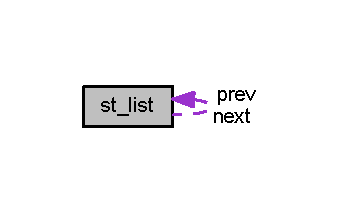
\includegraphics[width=162pt]{structst__list__coll__graph}
\end{center}
\end{figure}
\subsection*{Data Fields}
\begin{DoxyCompactItemize}
\item 
struct \hyperlink{structst__list}{st\+\_\+list} $\ast$ \hyperlink{structst__list_a53506b20583b3dfd486ff9f60f1450da}{prev}
\item 
struct \hyperlink{structst__list}{st\+\_\+list} $\ast$ \hyperlink{structst__list_a2df21777b3d410ab0803ee9046b3764e}{next}
\item 
void $\ast$ \hyperlink{structst__list_a178fcbad1f7324818b3da52be702e8dd}{data}
\end{DoxyCompactItemize}


\subsection{Field Documentation}
\hypertarget{structst__list_a178fcbad1f7324818b3da52be702e8dd}{}\index{st\+\_\+list@{st\+\_\+list}!data@{data}}
\index{data@{data}!st\+\_\+list@{st\+\_\+list}}
\subsubsection[{data}]{\setlength{\rightskip}{0pt plus 5cm}void$\ast$ st\+\_\+list\+::data}\label{structst__list_a178fcbad1f7324818b3da52be702e8dd}
\hypertarget{structst__list_a2df21777b3d410ab0803ee9046b3764e}{}\index{st\+\_\+list@{st\+\_\+list}!next@{next}}
\index{next@{next}!st\+\_\+list@{st\+\_\+list}}
\subsubsection[{next}]{\setlength{\rightskip}{0pt plus 5cm}struct {\bf st\+\_\+list} $\ast$ st\+\_\+list\+::next}\label{structst__list_a2df21777b3d410ab0803ee9046b3764e}
\hypertarget{structst__list_a53506b20583b3dfd486ff9f60f1450da}{}\index{st\+\_\+list@{st\+\_\+list}!prev@{prev}}
\index{prev@{prev}!st\+\_\+list@{st\+\_\+list}}
\subsubsection[{prev}]{\setlength{\rightskip}{0pt plus 5cm}struct {\bf st\+\_\+list}$\ast$ st\+\_\+list\+::prev}\label{structst__list_a53506b20583b3dfd486ff9f60f1450da}


The documentation for this struct was generated from the following file\+:\begin{DoxyCompactItemize}
\item 
\hyperlink{my__list_8h}{my\+\_\+list.\+h}\end{DoxyCompactItemize}

\hypertarget{structst__mem__root}{}\section{st\+\_\+mem\+\_\+root Struct Reference}
\label{structst__mem__root}\index{st\+\_\+mem\+\_\+root@{st\+\_\+mem\+\_\+root}}


{\ttfamily \#include $<$my\+\_\+alloc.\+h$>$}



Collaboration diagram for st\+\_\+mem\+\_\+root\+:\nopagebreak
\begin{figure}[H]
\begin{center}
\leavevmode
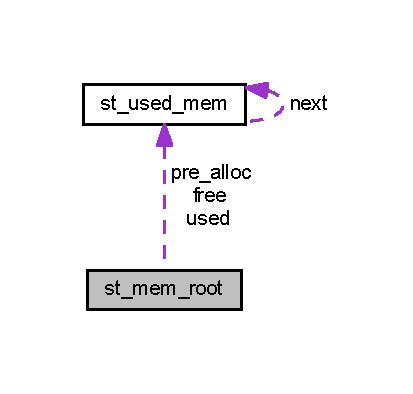
\includegraphics[width=198pt]{structst__mem__root__coll__graph}
\end{center}
\end{figure}
\subsection*{Data Fields}
\begin{DoxyCompactItemize}
\item 
\hyperlink{my__alloc_8h_adcee356751476eb8212d707ab71a525c}{U\+S\+E\+D\+\_\+\+M\+E\+M} $\ast$ \hyperlink{structst__mem__root_a589eeca4f55433bbbce712b16d437d9b}{free}
\item 
\hyperlink{my__alloc_8h_adcee356751476eb8212d707ab71a525c}{U\+S\+E\+D\+\_\+\+M\+E\+M} $\ast$ \hyperlink{structst__mem__root_a119bc46a5b34383d7a82c32d7c1b9077}{used}
\item 
\hyperlink{my__alloc_8h_adcee356751476eb8212d707ab71a525c}{U\+S\+E\+D\+\_\+\+M\+E\+M} $\ast$ \hyperlink{structst__mem__root_ac93aa644c9eae6a4260929234d460117}{pre\+\_\+alloc}
\item 
size\+\_\+t \hyperlink{structst__mem__root_ae20a32941b57232d2fcf86e94ebb289e}{min\+\_\+malloc}
\item 
size\+\_\+t \hyperlink{structst__mem__root_a719ac747366fcfeef5dbd164fceaacdd}{block\+\_\+size}
\item 
unsigned int \hyperlink{structst__mem__root_a67bc70b3e0703bbab62a143ba407ddb8}{block\+\_\+num}
\item 
unsigned int \hyperlink{structst__mem__root_a6d11a091d78fba6e427962ed2521d048}{first\+\_\+block\+\_\+usage}
\item 
void($\ast$ \hyperlink{structst__mem__root_aed812c144fbd9a5f1281e693729db75d}{error\+\_\+handler} )(void)
\item 
P\+S\+I\+\_\+memory\+\_\+key \hyperlink{structst__mem__root_afd13e15db0a42ca22e6f20c33d4e9fb3}{m\+\_\+psi\+\_\+key}
\end{DoxyCompactItemize}


\subsection{Field Documentation}
\hypertarget{structst__mem__root_a67bc70b3e0703bbab62a143ba407ddb8}{}\index{st\+\_\+mem\+\_\+root@{st\+\_\+mem\+\_\+root}!block\+\_\+num@{block\+\_\+num}}
\index{block\+\_\+num@{block\+\_\+num}!st\+\_\+mem\+\_\+root@{st\+\_\+mem\+\_\+root}}
\subsubsection[{block\+\_\+num}]{\setlength{\rightskip}{0pt plus 5cm}unsigned int st\+\_\+mem\+\_\+root\+::block\+\_\+num}\label{structst__mem__root_a67bc70b3e0703bbab62a143ba407ddb8}
\hypertarget{structst__mem__root_a719ac747366fcfeef5dbd164fceaacdd}{}\index{st\+\_\+mem\+\_\+root@{st\+\_\+mem\+\_\+root}!block\+\_\+size@{block\+\_\+size}}
\index{block\+\_\+size@{block\+\_\+size}!st\+\_\+mem\+\_\+root@{st\+\_\+mem\+\_\+root}}
\subsubsection[{block\+\_\+size}]{\setlength{\rightskip}{0pt plus 5cm}size\+\_\+t st\+\_\+mem\+\_\+root\+::block\+\_\+size}\label{structst__mem__root_a719ac747366fcfeef5dbd164fceaacdd}
\hypertarget{structst__mem__root_aed812c144fbd9a5f1281e693729db75d}{}\index{st\+\_\+mem\+\_\+root@{st\+\_\+mem\+\_\+root}!error\+\_\+handler@{error\+\_\+handler}}
\index{error\+\_\+handler@{error\+\_\+handler}!st\+\_\+mem\+\_\+root@{st\+\_\+mem\+\_\+root}}
\subsubsection[{error\+\_\+handler}]{\setlength{\rightskip}{0pt plus 5cm}void($\ast$ st\+\_\+mem\+\_\+root\+::error\+\_\+handler) (void)}\label{structst__mem__root_aed812c144fbd9a5f1281e693729db75d}
\hypertarget{structst__mem__root_a6d11a091d78fba6e427962ed2521d048}{}\index{st\+\_\+mem\+\_\+root@{st\+\_\+mem\+\_\+root}!first\+\_\+block\+\_\+usage@{first\+\_\+block\+\_\+usage}}
\index{first\+\_\+block\+\_\+usage@{first\+\_\+block\+\_\+usage}!st\+\_\+mem\+\_\+root@{st\+\_\+mem\+\_\+root}}
\subsubsection[{first\+\_\+block\+\_\+usage}]{\setlength{\rightskip}{0pt plus 5cm}unsigned int st\+\_\+mem\+\_\+root\+::first\+\_\+block\+\_\+usage}\label{structst__mem__root_a6d11a091d78fba6e427962ed2521d048}
\hypertarget{structst__mem__root_a589eeca4f55433bbbce712b16d437d9b}{}\index{st\+\_\+mem\+\_\+root@{st\+\_\+mem\+\_\+root}!free@{free}}
\index{free@{free}!st\+\_\+mem\+\_\+root@{st\+\_\+mem\+\_\+root}}
\subsubsection[{free}]{\setlength{\rightskip}{0pt plus 5cm}{\bf U\+S\+E\+D\+\_\+\+M\+E\+M}$\ast$ st\+\_\+mem\+\_\+root\+::free}\label{structst__mem__root_a589eeca4f55433bbbce712b16d437d9b}
\hypertarget{structst__mem__root_afd13e15db0a42ca22e6f20c33d4e9fb3}{}\index{st\+\_\+mem\+\_\+root@{st\+\_\+mem\+\_\+root}!m\+\_\+psi\+\_\+key@{m\+\_\+psi\+\_\+key}}
\index{m\+\_\+psi\+\_\+key@{m\+\_\+psi\+\_\+key}!st\+\_\+mem\+\_\+root@{st\+\_\+mem\+\_\+root}}
\subsubsection[{m\+\_\+psi\+\_\+key}]{\setlength{\rightskip}{0pt plus 5cm}P\+S\+I\+\_\+memory\+\_\+key st\+\_\+mem\+\_\+root\+::m\+\_\+psi\+\_\+key}\label{structst__mem__root_afd13e15db0a42ca22e6f20c33d4e9fb3}
\hypertarget{structst__mem__root_ae20a32941b57232d2fcf86e94ebb289e}{}\index{st\+\_\+mem\+\_\+root@{st\+\_\+mem\+\_\+root}!min\+\_\+malloc@{min\+\_\+malloc}}
\index{min\+\_\+malloc@{min\+\_\+malloc}!st\+\_\+mem\+\_\+root@{st\+\_\+mem\+\_\+root}}
\subsubsection[{min\+\_\+malloc}]{\setlength{\rightskip}{0pt plus 5cm}size\+\_\+t st\+\_\+mem\+\_\+root\+::min\+\_\+malloc}\label{structst__mem__root_ae20a32941b57232d2fcf86e94ebb289e}
\hypertarget{structst__mem__root_ac93aa644c9eae6a4260929234d460117}{}\index{st\+\_\+mem\+\_\+root@{st\+\_\+mem\+\_\+root}!pre\+\_\+alloc@{pre\+\_\+alloc}}
\index{pre\+\_\+alloc@{pre\+\_\+alloc}!st\+\_\+mem\+\_\+root@{st\+\_\+mem\+\_\+root}}
\subsubsection[{pre\+\_\+alloc}]{\setlength{\rightskip}{0pt plus 5cm}{\bf U\+S\+E\+D\+\_\+\+M\+E\+M}$\ast$ st\+\_\+mem\+\_\+root\+::pre\+\_\+alloc}\label{structst__mem__root_ac93aa644c9eae6a4260929234d460117}
\hypertarget{structst__mem__root_a119bc46a5b34383d7a82c32d7c1b9077}{}\index{st\+\_\+mem\+\_\+root@{st\+\_\+mem\+\_\+root}!used@{used}}
\index{used@{used}!st\+\_\+mem\+\_\+root@{st\+\_\+mem\+\_\+root}}
\subsubsection[{used}]{\setlength{\rightskip}{0pt plus 5cm}{\bf U\+S\+E\+D\+\_\+\+M\+E\+M}$\ast$ st\+\_\+mem\+\_\+root\+::used}\label{structst__mem__root_a119bc46a5b34383d7a82c32d7c1b9077}


The documentation for this struct was generated from the following file\+:\begin{DoxyCompactItemize}
\item 
\hyperlink{my__alloc_8h}{my\+\_\+alloc.\+h}\end{DoxyCompactItemize}

\hypertarget{structst__mysql}{}\section{st\+\_\+mysql Struct Reference}
\label{structst__mysql}\index{st\+\_\+mysql@{st\+\_\+mysql}}


{\ttfamily \#include $<$mysql.\+h$>$}



Collaboration diagram for st\+\_\+mysql\+:\nopagebreak
\begin{figure}[H]
\begin{center}
\leavevmode
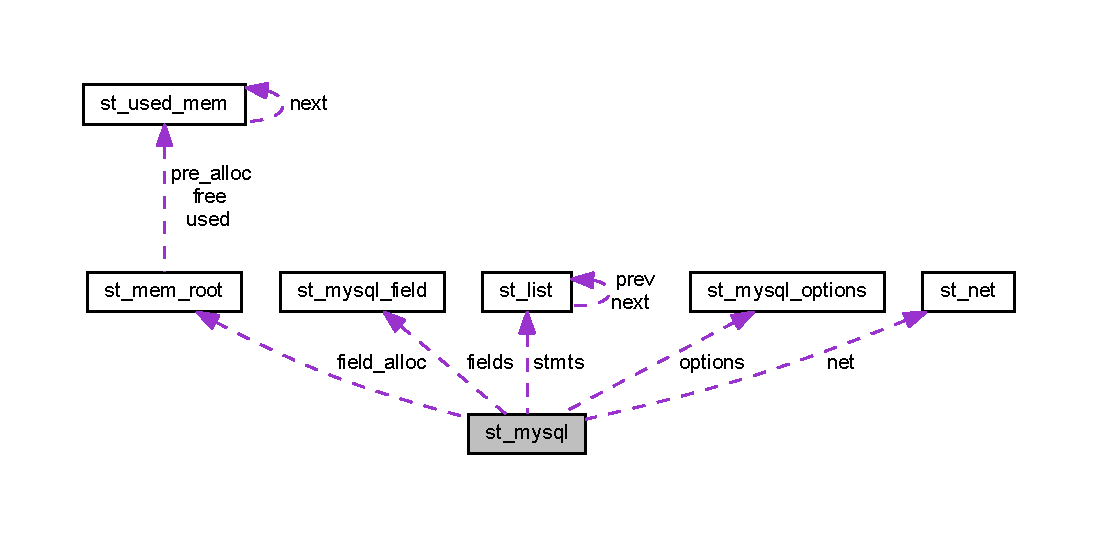
\includegraphics[width=350pt]{structst__mysql__coll__graph}
\end{center}
\end{figure}
\subsection*{Data Fields}
\begin{DoxyCompactItemize}
\item 
\hyperlink{mysql__com_8h_a6869c9fe9e26bbedea92d6603825d482}{N\+E\+T} \hyperlink{structst__mysql_a4ad66660f7b58712cb4bcaa852d4048c}{net}
\item 
unsigned char $\ast$ \hyperlink{structst__mysql_a88b1d70cf9bc81ce088f0a3418d6429c}{connector\+\_\+fd}
\item 
char $\ast$ \hyperlink{structst__mysql_aa63af77ef72c5732d53d735a67d20714}{host}
\item 
char $\ast$ \hyperlink{structst__mysql_ad5bf53f25b64492bee18c140c11081b6}{user}
\item 
char $\ast$ \hyperlink{structst__mysql_a63e75633e001c08953663a632819b285}{passwd}
\item 
char $\ast$ \hyperlink{structst__mysql_a1a1abcf3441139031de0aa767207dc6a}{unix\+\_\+socket}
\item 
char $\ast$ \hyperlink{structst__mysql_a72928c42be914f8c12aa24331c542b69}{server\+\_\+version}
\item 
char $\ast$ \hyperlink{structst__mysql_afcd1b31ab175617ee15a9c26a6258457}{host\+\_\+info}
\item 
char $\ast$ \hyperlink{structst__mysql_acd1bb786ff93e6a27ec5028864945a5a}{info}
\item 
char $\ast$ \hyperlink{structst__mysql_add1f635a8aea354868cfe57dba0d6298}{db}
\item 
struct charset\+\_\+info\+\_\+st $\ast$ \hyperlink{structst__mysql_a5d128ecd21c6265f37c283824b3ad813}{charset}
\item 
\hyperlink{mysql_8h_ad010774d7ae34dc28a2e044ed2cd4f71}{M\+Y\+S\+Q\+L\+\_\+\+F\+I\+E\+L\+D} $\ast$ \hyperlink{structst__mysql_aa31b4c644fcef355ce347977a47be9b2}{fields}
\item 
\hyperlink{my__alloc_8h_ac59e289b254a2c5ac634ffcedda3f823}{M\+E\+M\+\_\+\+R\+O\+O\+T} \hyperlink{structst__mysql_a170585335f5edffeaae3f5229f6c1f6b}{field\+\_\+alloc}
\item 
\hyperlink{mysql_8h_ae05bd5d3e5a75578e2f14cfeb43f07aa}{my\+\_\+ulonglong} \hyperlink{structst__mysql_acf6930c0bcb39cc19665b1a4142ba559}{affected\+\_\+rows}
\item 
\hyperlink{mysql_8h_ae05bd5d3e5a75578e2f14cfeb43f07aa}{my\+\_\+ulonglong} \hyperlink{structst__mysql_a884df86e03be14c772cfe48511963fc1}{insert\+\_\+id}
\item 
\hyperlink{mysql_8h_ae05bd5d3e5a75578e2f14cfeb43f07aa}{my\+\_\+ulonglong} \hyperlink{structst__mysql_ab70022082b9c53ab9c9fc8b966ad2d8a}{extra\+\_\+info}
\item 
unsigned long \hyperlink{structst__mysql_a9f32d330dbd811f50b7440786febb25f}{thread\+\_\+id}
\item 
unsigned long \hyperlink{structst__mysql_afa6ee000a88fe95750c9f1acd9711023}{packet\+\_\+length}
\item 
unsigned int \hyperlink{structst__mysql_a285c6023c0903a47d4e6cdebde4c6dfe}{port}
\item 
unsigned long \hyperlink{structst__mysql_af572471668d07fd887bc68d44375d8a5}{client\+\_\+flag}
\item 
unsigned long \hyperlink{structst__mysql_ab9c7460496350f7aa331c104aa54717d}{server\+\_\+capabilities}
\item 
unsigned int \hyperlink{structst__mysql_a43e5c1629a6db251dc9b5d4eecceb209}{protocol\+\_\+version}
\item 
unsigned int \hyperlink{structst__mysql_a7bedc1452ea1a2b76634e92196a02991}{field\+\_\+count}
\item 
unsigned int \hyperlink{structst__mysql_ab875d849ff6f754a85986fe538408667}{server\+\_\+status}
\item 
unsigned int \hyperlink{structst__mysql_a855f117151afa573d46f988e2e01393a}{server\+\_\+language}
\item 
unsigned int \hyperlink{structst__mysql_a397568fcafb4431f45aaddce083d680e}{warning\+\_\+count}
\item 
struct \hyperlink{structst__mysql__options}{st\+\_\+mysql\+\_\+options} \hyperlink{structst__mysql_af5b1e7032c012c17dbb967fa4ac212a9}{options}
\item 
enum \hyperlink{mysql_8h_a8c0cf7afc762670cf296e4a0067cae5d}{mysql\+\_\+status} \hyperlink{structst__mysql_abd3b5b4aa083403f1025f688731b196e}{status}
\item 
\hyperlink{mysql_8h_a74cd599039dcf29c6e6d342cf4efd0a8}{my\+\_\+bool} \hyperlink{structst__mysql_a360756ba79af768da73d528969759b64}{free\+\_\+me}
\item 
\hyperlink{mysql_8h_a74cd599039dcf29c6e6d342cf4efd0a8}{my\+\_\+bool} \hyperlink{structst__mysql_a802266361a427c12d6cb29a27f8889b1}{reconnect}
\item 
char \hyperlink{structst__mysql_ae6e34dfb59ec6f6842f65a58eb6bee38}{scramble} \mbox{[}\hyperlink{mysql__com_8h_a45f11cf97b6dec62756b92cbb96f7418}{S\+C\+R\+A\+M\+B\+L\+E\+\_\+\+L\+E\+N\+G\+T\+H}+1\mbox{]}
\item 
\hyperlink{mysql_8h_a74cd599039dcf29c6e6d342cf4efd0a8}{my\+\_\+bool} \hyperlink{structst__mysql_aa9656f1c38e91c63a2c7b86144e9e675}{unused1}
\item 
void $\ast$ \hyperlink{structst__mysql_ae0451f85e4dcfd3acf69235f20febc75}{unused2}
\item 
void $\ast$ \hyperlink{structst__mysql_abbe6315ea3e9df0e9e1d93708e31da56}{unused3}
\item 
void $\ast$ \hyperlink{structst__mysql_a2887d342b67605530757845522c307be}{unused4}
\item 
void $\ast$ \hyperlink{structst__mysql_af3adab90c86872eff4b923469b459749}{unused5}
\item 
\hyperlink{my__list_8h_ab2a1c5fd766481fe9ec169b9fdca184e}{L\+I\+S\+T} $\ast$ \hyperlink{structst__mysql_afe0722884084a6d3a8b9448e71ca25e2}{stmts}
\item 
const struct st\+\_\+mysql\+\_\+methods $\ast$ \hyperlink{structst__mysql_a04129bc0cbeda076db8ba274ed93328d}{methods}
\item 
void $\ast$ \hyperlink{structst__mysql_af7c6f25aed31575514966a3cdf77ebc6}{thd}
\item 
\hyperlink{mysql_8h_a74cd599039dcf29c6e6d342cf4efd0a8}{my\+\_\+bool} $\ast$ \hyperlink{structst__mysql_a7245af2550c3858f3e2e22c55538f7e1}{unbuffered\+\_\+fetch\+\_\+owner}
\item 
char $\ast$ \hyperlink{structst__mysql_a135e9fa0dea39f54be633acd845634a4}{info\+\_\+buffer}
\item 
void $\ast$ \hyperlink{structst__mysql_a544142924a78d2fb3f7bbda547fc5a14}{extension}
\end{DoxyCompactItemize}


\subsection{Field Documentation}
\hypertarget{structst__mysql_acf6930c0bcb39cc19665b1a4142ba559}{}\index{st\+\_\+mysql@{st\+\_\+mysql}!affected\+\_\+rows@{affected\+\_\+rows}}
\index{affected\+\_\+rows@{affected\+\_\+rows}!st\+\_\+mysql@{st\+\_\+mysql}}
\subsubsection[{affected\+\_\+rows}]{\setlength{\rightskip}{0pt plus 5cm}{\bf my\+\_\+ulonglong} st\+\_\+mysql\+::affected\+\_\+rows}\label{structst__mysql_acf6930c0bcb39cc19665b1a4142ba559}
\hypertarget{structst__mysql_a5d128ecd21c6265f37c283824b3ad813}{}\index{st\+\_\+mysql@{st\+\_\+mysql}!charset@{charset}}
\index{charset@{charset}!st\+\_\+mysql@{st\+\_\+mysql}}
\subsubsection[{charset}]{\setlength{\rightskip}{0pt plus 5cm}struct charset\+\_\+info\+\_\+st$\ast$ st\+\_\+mysql\+::charset}\label{structst__mysql_a5d128ecd21c6265f37c283824b3ad813}
\hypertarget{structst__mysql_af572471668d07fd887bc68d44375d8a5}{}\index{st\+\_\+mysql@{st\+\_\+mysql}!client\+\_\+flag@{client\+\_\+flag}}
\index{client\+\_\+flag@{client\+\_\+flag}!st\+\_\+mysql@{st\+\_\+mysql}}
\subsubsection[{client\+\_\+flag}]{\setlength{\rightskip}{0pt plus 5cm}unsigned long st\+\_\+mysql\+::client\+\_\+flag}\label{structst__mysql_af572471668d07fd887bc68d44375d8a5}
\hypertarget{structst__mysql_a88b1d70cf9bc81ce088f0a3418d6429c}{}\index{st\+\_\+mysql@{st\+\_\+mysql}!connector\+\_\+fd@{connector\+\_\+fd}}
\index{connector\+\_\+fd@{connector\+\_\+fd}!st\+\_\+mysql@{st\+\_\+mysql}}
\subsubsection[{connector\+\_\+fd}]{\setlength{\rightskip}{0pt plus 5cm}unsigned char$\ast$ st\+\_\+mysql\+::connector\+\_\+fd}\label{structst__mysql_a88b1d70cf9bc81ce088f0a3418d6429c}
\hypertarget{structst__mysql_add1f635a8aea354868cfe57dba0d6298}{}\index{st\+\_\+mysql@{st\+\_\+mysql}!db@{db}}
\index{db@{db}!st\+\_\+mysql@{st\+\_\+mysql}}
\subsubsection[{db}]{\setlength{\rightskip}{0pt plus 5cm}char $\ast$ st\+\_\+mysql\+::db}\label{structst__mysql_add1f635a8aea354868cfe57dba0d6298}
\hypertarget{structst__mysql_a544142924a78d2fb3f7bbda547fc5a14}{}\index{st\+\_\+mysql@{st\+\_\+mysql}!extension@{extension}}
\index{extension@{extension}!st\+\_\+mysql@{st\+\_\+mysql}}
\subsubsection[{extension}]{\setlength{\rightskip}{0pt plus 5cm}void$\ast$ st\+\_\+mysql\+::extension}\label{structst__mysql_a544142924a78d2fb3f7bbda547fc5a14}
\hypertarget{structst__mysql_ab70022082b9c53ab9c9fc8b966ad2d8a}{}\index{st\+\_\+mysql@{st\+\_\+mysql}!extra\+\_\+info@{extra\+\_\+info}}
\index{extra\+\_\+info@{extra\+\_\+info}!st\+\_\+mysql@{st\+\_\+mysql}}
\subsubsection[{extra\+\_\+info}]{\setlength{\rightskip}{0pt plus 5cm}{\bf my\+\_\+ulonglong} st\+\_\+mysql\+::extra\+\_\+info}\label{structst__mysql_ab70022082b9c53ab9c9fc8b966ad2d8a}
\hypertarget{structst__mysql_a170585335f5edffeaae3f5229f6c1f6b}{}\index{st\+\_\+mysql@{st\+\_\+mysql}!field\+\_\+alloc@{field\+\_\+alloc}}
\index{field\+\_\+alloc@{field\+\_\+alloc}!st\+\_\+mysql@{st\+\_\+mysql}}
\subsubsection[{field\+\_\+alloc}]{\setlength{\rightskip}{0pt plus 5cm}{\bf M\+E\+M\+\_\+\+R\+O\+O\+T} st\+\_\+mysql\+::field\+\_\+alloc}\label{structst__mysql_a170585335f5edffeaae3f5229f6c1f6b}
\hypertarget{structst__mysql_a7bedc1452ea1a2b76634e92196a02991}{}\index{st\+\_\+mysql@{st\+\_\+mysql}!field\+\_\+count@{field\+\_\+count}}
\index{field\+\_\+count@{field\+\_\+count}!st\+\_\+mysql@{st\+\_\+mysql}}
\subsubsection[{field\+\_\+count}]{\setlength{\rightskip}{0pt plus 5cm}unsigned int st\+\_\+mysql\+::field\+\_\+count}\label{structst__mysql_a7bedc1452ea1a2b76634e92196a02991}
\hypertarget{structst__mysql_aa31b4c644fcef355ce347977a47be9b2}{}\index{st\+\_\+mysql@{st\+\_\+mysql}!fields@{fields}}
\index{fields@{fields}!st\+\_\+mysql@{st\+\_\+mysql}}
\subsubsection[{fields}]{\setlength{\rightskip}{0pt plus 5cm}{\bf M\+Y\+S\+Q\+L\+\_\+\+F\+I\+E\+L\+D}$\ast$ st\+\_\+mysql\+::fields}\label{structst__mysql_aa31b4c644fcef355ce347977a47be9b2}
\hypertarget{structst__mysql_a360756ba79af768da73d528969759b64}{}\index{st\+\_\+mysql@{st\+\_\+mysql}!free\+\_\+me@{free\+\_\+me}}
\index{free\+\_\+me@{free\+\_\+me}!st\+\_\+mysql@{st\+\_\+mysql}}
\subsubsection[{free\+\_\+me}]{\setlength{\rightskip}{0pt plus 5cm}{\bf my\+\_\+bool} st\+\_\+mysql\+::free\+\_\+me}\label{structst__mysql_a360756ba79af768da73d528969759b64}
\hypertarget{structst__mysql_aa63af77ef72c5732d53d735a67d20714}{}\index{st\+\_\+mysql@{st\+\_\+mysql}!host@{host}}
\index{host@{host}!st\+\_\+mysql@{st\+\_\+mysql}}
\subsubsection[{host}]{\setlength{\rightskip}{0pt plus 5cm}char$\ast$ st\+\_\+mysql\+::host}\label{structst__mysql_aa63af77ef72c5732d53d735a67d20714}
\hypertarget{structst__mysql_afcd1b31ab175617ee15a9c26a6258457}{}\index{st\+\_\+mysql@{st\+\_\+mysql}!host\+\_\+info@{host\+\_\+info}}
\index{host\+\_\+info@{host\+\_\+info}!st\+\_\+mysql@{st\+\_\+mysql}}
\subsubsection[{host\+\_\+info}]{\setlength{\rightskip}{0pt plus 5cm}char $\ast$ st\+\_\+mysql\+::host\+\_\+info}\label{structst__mysql_afcd1b31ab175617ee15a9c26a6258457}
\hypertarget{structst__mysql_acd1bb786ff93e6a27ec5028864945a5a}{}\index{st\+\_\+mysql@{st\+\_\+mysql}!info@{info}}
\index{info@{info}!st\+\_\+mysql@{st\+\_\+mysql}}
\subsubsection[{info}]{\setlength{\rightskip}{0pt plus 5cm}char$\ast$ st\+\_\+mysql\+::info}\label{structst__mysql_acd1bb786ff93e6a27ec5028864945a5a}
\hypertarget{structst__mysql_a135e9fa0dea39f54be633acd845634a4}{}\index{st\+\_\+mysql@{st\+\_\+mysql}!info\+\_\+buffer@{info\+\_\+buffer}}
\index{info\+\_\+buffer@{info\+\_\+buffer}!st\+\_\+mysql@{st\+\_\+mysql}}
\subsubsection[{info\+\_\+buffer}]{\setlength{\rightskip}{0pt plus 5cm}char$\ast$ st\+\_\+mysql\+::info\+\_\+buffer}\label{structst__mysql_a135e9fa0dea39f54be633acd845634a4}
\hypertarget{structst__mysql_a884df86e03be14c772cfe48511963fc1}{}\index{st\+\_\+mysql@{st\+\_\+mysql}!insert\+\_\+id@{insert\+\_\+id}}
\index{insert\+\_\+id@{insert\+\_\+id}!st\+\_\+mysql@{st\+\_\+mysql}}
\subsubsection[{insert\+\_\+id}]{\setlength{\rightskip}{0pt plus 5cm}{\bf my\+\_\+ulonglong} st\+\_\+mysql\+::insert\+\_\+id}\label{structst__mysql_a884df86e03be14c772cfe48511963fc1}
\hypertarget{structst__mysql_a04129bc0cbeda076db8ba274ed93328d}{}\index{st\+\_\+mysql@{st\+\_\+mysql}!methods@{methods}}
\index{methods@{methods}!st\+\_\+mysql@{st\+\_\+mysql}}
\subsubsection[{methods}]{\setlength{\rightskip}{0pt plus 5cm}const struct st\+\_\+mysql\+\_\+methods$\ast$ st\+\_\+mysql\+::methods}\label{structst__mysql_a04129bc0cbeda076db8ba274ed93328d}
\hypertarget{structst__mysql_a4ad66660f7b58712cb4bcaa852d4048c}{}\index{st\+\_\+mysql@{st\+\_\+mysql}!net@{net}}
\index{net@{net}!st\+\_\+mysql@{st\+\_\+mysql}}
\subsubsection[{net}]{\setlength{\rightskip}{0pt plus 5cm}{\bf N\+E\+T} st\+\_\+mysql\+::net}\label{structst__mysql_a4ad66660f7b58712cb4bcaa852d4048c}
\hypertarget{structst__mysql_af5b1e7032c012c17dbb967fa4ac212a9}{}\index{st\+\_\+mysql@{st\+\_\+mysql}!options@{options}}
\index{options@{options}!st\+\_\+mysql@{st\+\_\+mysql}}
\subsubsection[{options}]{\setlength{\rightskip}{0pt plus 5cm}struct {\bf st\+\_\+mysql\+\_\+options} st\+\_\+mysql\+::options}\label{structst__mysql_af5b1e7032c012c17dbb967fa4ac212a9}
\hypertarget{structst__mysql_afa6ee000a88fe95750c9f1acd9711023}{}\index{st\+\_\+mysql@{st\+\_\+mysql}!packet\+\_\+length@{packet\+\_\+length}}
\index{packet\+\_\+length@{packet\+\_\+length}!st\+\_\+mysql@{st\+\_\+mysql}}
\subsubsection[{packet\+\_\+length}]{\setlength{\rightskip}{0pt plus 5cm}unsigned long st\+\_\+mysql\+::packet\+\_\+length}\label{structst__mysql_afa6ee000a88fe95750c9f1acd9711023}
\hypertarget{structst__mysql_a63e75633e001c08953663a632819b285}{}\index{st\+\_\+mysql@{st\+\_\+mysql}!passwd@{passwd}}
\index{passwd@{passwd}!st\+\_\+mysql@{st\+\_\+mysql}}
\subsubsection[{passwd}]{\setlength{\rightskip}{0pt plus 5cm}char $\ast$ st\+\_\+mysql\+::passwd}\label{structst__mysql_a63e75633e001c08953663a632819b285}
\hypertarget{structst__mysql_a285c6023c0903a47d4e6cdebde4c6dfe}{}\index{st\+\_\+mysql@{st\+\_\+mysql}!port@{port}}
\index{port@{port}!st\+\_\+mysql@{st\+\_\+mysql}}
\subsubsection[{port}]{\setlength{\rightskip}{0pt plus 5cm}unsigned int st\+\_\+mysql\+::port}\label{structst__mysql_a285c6023c0903a47d4e6cdebde4c6dfe}
\hypertarget{structst__mysql_a43e5c1629a6db251dc9b5d4eecceb209}{}\index{st\+\_\+mysql@{st\+\_\+mysql}!protocol\+\_\+version@{protocol\+\_\+version}}
\index{protocol\+\_\+version@{protocol\+\_\+version}!st\+\_\+mysql@{st\+\_\+mysql}}
\subsubsection[{protocol\+\_\+version}]{\setlength{\rightskip}{0pt plus 5cm}unsigned int st\+\_\+mysql\+::protocol\+\_\+version}\label{structst__mysql_a43e5c1629a6db251dc9b5d4eecceb209}
\hypertarget{structst__mysql_a802266361a427c12d6cb29a27f8889b1}{}\index{st\+\_\+mysql@{st\+\_\+mysql}!reconnect@{reconnect}}
\index{reconnect@{reconnect}!st\+\_\+mysql@{st\+\_\+mysql}}
\subsubsection[{reconnect}]{\setlength{\rightskip}{0pt plus 5cm}{\bf my\+\_\+bool} st\+\_\+mysql\+::reconnect}\label{structst__mysql_a802266361a427c12d6cb29a27f8889b1}
\hypertarget{structst__mysql_ae6e34dfb59ec6f6842f65a58eb6bee38}{}\index{st\+\_\+mysql@{st\+\_\+mysql}!scramble@{scramble}}
\index{scramble@{scramble}!st\+\_\+mysql@{st\+\_\+mysql}}
\subsubsection[{scramble}]{\setlength{\rightskip}{0pt plus 5cm}char st\+\_\+mysql\+::scramble\mbox{[}{\bf S\+C\+R\+A\+M\+B\+L\+E\+\_\+\+L\+E\+N\+G\+T\+H}+1\mbox{]}}\label{structst__mysql_ae6e34dfb59ec6f6842f65a58eb6bee38}
\hypertarget{structst__mysql_ab9c7460496350f7aa331c104aa54717d}{}\index{st\+\_\+mysql@{st\+\_\+mysql}!server\+\_\+capabilities@{server\+\_\+capabilities}}
\index{server\+\_\+capabilities@{server\+\_\+capabilities}!st\+\_\+mysql@{st\+\_\+mysql}}
\subsubsection[{server\+\_\+capabilities}]{\setlength{\rightskip}{0pt plus 5cm}unsigned long st\+\_\+mysql\+::server\+\_\+capabilities}\label{structst__mysql_ab9c7460496350f7aa331c104aa54717d}
\hypertarget{structst__mysql_a855f117151afa573d46f988e2e01393a}{}\index{st\+\_\+mysql@{st\+\_\+mysql}!server\+\_\+language@{server\+\_\+language}}
\index{server\+\_\+language@{server\+\_\+language}!st\+\_\+mysql@{st\+\_\+mysql}}
\subsubsection[{server\+\_\+language}]{\setlength{\rightskip}{0pt plus 5cm}unsigned int st\+\_\+mysql\+::server\+\_\+language}\label{structst__mysql_a855f117151afa573d46f988e2e01393a}
\hypertarget{structst__mysql_ab875d849ff6f754a85986fe538408667}{}\index{st\+\_\+mysql@{st\+\_\+mysql}!server\+\_\+status@{server\+\_\+status}}
\index{server\+\_\+status@{server\+\_\+status}!st\+\_\+mysql@{st\+\_\+mysql}}
\subsubsection[{server\+\_\+status}]{\setlength{\rightskip}{0pt plus 5cm}unsigned int st\+\_\+mysql\+::server\+\_\+status}\label{structst__mysql_ab875d849ff6f754a85986fe538408667}
\hypertarget{structst__mysql_a72928c42be914f8c12aa24331c542b69}{}\index{st\+\_\+mysql@{st\+\_\+mysql}!server\+\_\+version@{server\+\_\+version}}
\index{server\+\_\+version@{server\+\_\+version}!st\+\_\+mysql@{st\+\_\+mysql}}
\subsubsection[{server\+\_\+version}]{\setlength{\rightskip}{0pt plus 5cm}char $\ast$ st\+\_\+mysql\+::server\+\_\+version}\label{structst__mysql_a72928c42be914f8c12aa24331c542b69}
\hypertarget{structst__mysql_abd3b5b4aa083403f1025f688731b196e}{}\index{st\+\_\+mysql@{st\+\_\+mysql}!status@{status}}
\index{status@{status}!st\+\_\+mysql@{st\+\_\+mysql}}
\subsubsection[{status}]{\setlength{\rightskip}{0pt plus 5cm}enum {\bf mysql\+\_\+status} st\+\_\+mysql\+::status}\label{structst__mysql_abd3b5b4aa083403f1025f688731b196e}
\hypertarget{structst__mysql_afe0722884084a6d3a8b9448e71ca25e2}{}\index{st\+\_\+mysql@{st\+\_\+mysql}!stmts@{stmts}}
\index{stmts@{stmts}!st\+\_\+mysql@{st\+\_\+mysql}}
\subsubsection[{stmts}]{\setlength{\rightskip}{0pt plus 5cm}{\bf L\+I\+S\+T}$\ast$ st\+\_\+mysql\+::stmts}\label{structst__mysql_afe0722884084a6d3a8b9448e71ca25e2}
\hypertarget{structst__mysql_af7c6f25aed31575514966a3cdf77ebc6}{}\index{st\+\_\+mysql@{st\+\_\+mysql}!thd@{thd}}
\index{thd@{thd}!st\+\_\+mysql@{st\+\_\+mysql}}
\subsubsection[{thd}]{\setlength{\rightskip}{0pt plus 5cm}void$\ast$ st\+\_\+mysql\+::thd}\label{structst__mysql_af7c6f25aed31575514966a3cdf77ebc6}
\hypertarget{structst__mysql_a9f32d330dbd811f50b7440786febb25f}{}\index{st\+\_\+mysql@{st\+\_\+mysql}!thread\+\_\+id@{thread\+\_\+id}}
\index{thread\+\_\+id@{thread\+\_\+id}!st\+\_\+mysql@{st\+\_\+mysql}}
\subsubsection[{thread\+\_\+id}]{\setlength{\rightskip}{0pt plus 5cm}unsigned long st\+\_\+mysql\+::thread\+\_\+id}\label{structst__mysql_a9f32d330dbd811f50b7440786febb25f}
\hypertarget{structst__mysql_a7245af2550c3858f3e2e22c55538f7e1}{}\index{st\+\_\+mysql@{st\+\_\+mysql}!unbuffered\+\_\+fetch\+\_\+owner@{unbuffered\+\_\+fetch\+\_\+owner}}
\index{unbuffered\+\_\+fetch\+\_\+owner@{unbuffered\+\_\+fetch\+\_\+owner}!st\+\_\+mysql@{st\+\_\+mysql}}
\subsubsection[{unbuffered\+\_\+fetch\+\_\+owner}]{\setlength{\rightskip}{0pt plus 5cm}{\bf my\+\_\+bool}$\ast$ st\+\_\+mysql\+::unbuffered\+\_\+fetch\+\_\+owner}\label{structst__mysql_a7245af2550c3858f3e2e22c55538f7e1}
\hypertarget{structst__mysql_a1a1abcf3441139031de0aa767207dc6a}{}\index{st\+\_\+mysql@{st\+\_\+mysql}!unix\+\_\+socket@{unix\+\_\+socket}}
\index{unix\+\_\+socket@{unix\+\_\+socket}!st\+\_\+mysql@{st\+\_\+mysql}}
\subsubsection[{unix\+\_\+socket}]{\setlength{\rightskip}{0pt plus 5cm}char $\ast$ st\+\_\+mysql\+::unix\+\_\+socket}\label{structst__mysql_a1a1abcf3441139031de0aa767207dc6a}
\hypertarget{structst__mysql_aa9656f1c38e91c63a2c7b86144e9e675}{}\index{st\+\_\+mysql@{st\+\_\+mysql}!unused1@{unused1}}
\index{unused1@{unused1}!st\+\_\+mysql@{st\+\_\+mysql}}
\subsubsection[{unused1}]{\setlength{\rightskip}{0pt plus 5cm}{\bf my\+\_\+bool} st\+\_\+mysql\+::unused1}\label{structst__mysql_aa9656f1c38e91c63a2c7b86144e9e675}
\hypertarget{structst__mysql_ae0451f85e4dcfd3acf69235f20febc75}{}\index{st\+\_\+mysql@{st\+\_\+mysql}!unused2@{unused2}}
\index{unused2@{unused2}!st\+\_\+mysql@{st\+\_\+mysql}}
\subsubsection[{unused2}]{\setlength{\rightskip}{0pt plus 5cm}void$\ast$ st\+\_\+mysql\+::unused2}\label{structst__mysql_ae0451f85e4dcfd3acf69235f20febc75}
\hypertarget{structst__mysql_abbe6315ea3e9df0e9e1d93708e31da56}{}\index{st\+\_\+mysql@{st\+\_\+mysql}!unused3@{unused3}}
\index{unused3@{unused3}!st\+\_\+mysql@{st\+\_\+mysql}}
\subsubsection[{unused3}]{\setlength{\rightskip}{0pt plus 5cm}void $\ast$ st\+\_\+mysql\+::unused3}\label{structst__mysql_abbe6315ea3e9df0e9e1d93708e31da56}
\hypertarget{structst__mysql_a2887d342b67605530757845522c307be}{}\index{st\+\_\+mysql@{st\+\_\+mysql}!unused4@{unused4}}
\index{unused4@{unused4}!st\+\_\+mysql@{st\+\_\+mysql}}
\subsubsection[{unused4}]{\setlength{\rightskip}{0pt plus 5cm}void $\ast$ st\+\_\+mysql\+::unused4}\label{structst__mysql_a2887d342b67605530757845522c307be}
\hypertarget{structst__mysql_af3adab90c86872eff4b923469b459749}{}\index{st\+\_\+mysql@{st\+\_\+mysql}!unused5@{unused5}}
\index{unused5@{unused5}!st\+\_\+mysql@{st\+\_\+mysql}}
\subsubsection[{unused5}]{\setlength{\rightskip}{0pt plus 5cm}void $\ast$ st\+\_\+mysql\+::unused5}\label{structst__mysql_af3adab90c86872eff4b923469b459749}
\hypertarget{structst__mysql_ad5bf53f25b64492bee18c140c11081b6}{}\index{st\+\_\+mysql@{st\+\_\+mysql}!user@{user}}
\index{user@{user}!st\+\_\+mysql@{st\+\_\+mysql}}
\subsubsection[{user}]{\setlength{\rightskip}{0pt plus 5cm}char $\ast$ st\+\_\+mysql\+::user}\label{structst__mysql_ad5bf53f25b64492bee18c140c11081b6}
\hypertarget{structst__mysql_a397568fcafb4431f45aaddce083d680e}{}\index{st\+\_\+mysql@{st\+\_\+mysql}!warning\+\_\+count@{warning\+\_\+count}}
\index{warning\+\_\+count@{warning\+\_\+count}!st\+\_\+mysql@{st\+\_\+mysql}}
\subsubsection[{warning\+\_\+count}]{\setlength{\rightskip}{0pt plus 5cm}unsigned int st\+\_\+mysql\+::warning\+\_\+count}\label{structst__mysql_a397568fcafb4431f45aaddce083d680e}


The documentation for this struct was generated from the following file\+:\begin{DoxyCompactItemize}
\item 
\hyperlink{mysql_8h}{mysql.\+h}\end{DoxyCompactItemize}

\hypertarget{structst__mysql__bind}{}\section{st\+\_\+mysql\+\_\+bind Struct Reference}
\label{structst__mysql__bind}\index{st\+\_\+mysql\+\_\+bind@{st\+\_\+mysql\+\_\+bind}}


{\ttfamily \#include $<$mysql.\+h$>$}

\subsection*{Data Fields}
\begin{DoxyCompactItemize}
\item 
unsigned long $\ast$ \hyperlink{structst__mysql__bind_a255c7b483665c1d98aaf73606e72cfca}{length}
\item 
\hyperlink{mysql_8h_a74cd599039dcf29c6e6d342cf4efd0a8}{my\+\_\+bool} $\ast$ \hyperlink{structst__mysql__bind_a04defa2229677eefb0b50ed902358ef5}{is\+\_\+null}
\item 
void $\ast$ \hyperlink{structst__mysql__bind_a3ea4a5256c2e8c8f7b80ceea0ed5d3bb}{buffer}
\item 
\hyperlink{mysql_8h_a74cd599039dcf29c6e6d342cf4efd0a8}{my\+\_\+bool} $\ast$ \hyperlink{structst__mysql__bind_a555fb0921bc7a50e54c863b702a75259}{error}
\item 
unsigned char $\ast$ \hyperlink{structst__mysql__bind_a78b2414892e0e1af294bbf773dce201e}{row\+\_\+ptr}
\item 
void($\ast$ \hyperlink{structst__mysql__bind_ae7494004e650d528427e906727c22337}{store\+\_\+param\+\_\+func} )(\hyperlink{mysql__com_8h_a6869c9fe9e26bbedea92d6603825d482}{N\+E\+T} $\ast$net, struct \hyperlink{structst__mysql__bind}{st\+\_\+mysql\+\_\+bind} $\ast$param)
\item 
void($\ast$ \hyperlink{structst__mysql__bind_a1398006bc3b49e8a61084188976929ae}{fetch\+\_\+result} )(struct \hyperlink{structst__mysql__bind}{st\+\_\+mysql\+\_\+bind} $\ast$, \hyperlink{mysql_8h_ad010774d7ae34dc28a2e044ed2cd4f71}{M\+Y\+S\+Q\+L\+\_\+\+F\+I\+E\+L\+D} $\ast$, unsigned char $\ast$$\ast$row)
\item 
void($\ast$ \hyperlink{structst__mysql__bind_a5d9670e2a4c8dcc91f3d6b21fbc33e75}{skip\+\_\+result} )(struct \hyperlink{structst__mysql__bind}{st\+\_\+mysql\+\_\+bind} $\ast$, \hyperlink{mysql_8h_ad010774d7ae34dc28a2e044ed2cd4f71}{M\+Y\+S\+Q\+L\+\_\+\+F\+I\+E\+L\+D} $\ast$, unsigned char $\ast$$\ast$row)
\item 
unsigned long \hyperlink{structst__mysql__bind_a58fff187be9d3e492856a50f970b469f}{buffer\+\_\+length}
\item 
unsigned long \hyperlink{structst__mysql__bind_a5e786c095fb2f2c21167db2b08b2eb2a}{offset}
\item 
unsigned long \hyperlink{structst__mysql__bind_a3f78eab5d415489c5a0a6cb702974cf2}{length\+\_\+value}
\item 
unsigned int \hyperlink{structst__mysql__bind_a3d72263efdf64d9bf2eefe14588e35b3}{param\+\_\+number}
\item 
unsigned int \hyperlink{structst__mysql__bind_ae8961b4d8470d6e5b1b06d2c29e28170}{pack\+\_\+length}
\item 
enum \hyperlink{mysql__com_8h_a69e798807026a0f7e12b1d6c72374854}{enum\+\_\+field\+\_\+types} \hyperlink{structst__mysql__bind_ad3de66e824b46991edcc4ddbb3747ced}{buffer\+\_\+type}
\item 
\hyperlink{mysql_8h_a74cd599039dcf29c6e6d342cf4efd0a8}{my\+\_\+bool} \hyperlink{structst__mysql__bind_ac69cf2bf54564d646fbcf12c6981f18d}{error\+\_\+value}
\item 
\hyperlink{mysql_8h_a74cd599039dcf29c6e6d342cf4efd0a8}{my\+\_\+bool} \hyperlink{structst__mysql__bind_ae3a058be75cadc4f8219bbba9c322bad}{is\+\_\+unsigned}
\item 
\hyperlink{mysql_8h_a74cd599039dcf29c6e6d342cf4efd0a8}{my\+\_\+bool} \hyperlink{structst__mysql__bind_a31218c0f15b38ba638bcb302dcf50afb}{long\+\_\+data\+\_\+used}
\item 
\hyperlink{mysql_8h_a74cd599039dcf29c6e6d342cf4efd0a8}{my\+\_\+bool} \hyperlink{structst__mysql__bind_ae5b4c29062a979ed6039652301015a78}{is\+\_\+null\+\_\+value}
\item 
void $\ast$ \hyperlink{structst__mysql__bind_ac8e250bd8df7c1ff2921c3cb5c2ed564}{extension}
\end{DoxyCompactItemize}


\subsection{Field Documentation}
\hypertarget{structst__mysql__bind_a3ea4a5256c2e8c8f7b80ceea0ed5d3bb}{}\index{st\+\_\+mysql\+\_\+bind@{st\+\_\+mysql\+\_\+bind}!buffer@{buffer}}
\index{buffer@{buffer}!st\+\_\+mysql\+\_\+bind@{st\+\_\+mysql\+\_\+bind}}
\subsubsection[{buffer}]{\setlength{\rightskip}{0pt plus 5cm}void$\ast$ st\+\_\+mysql\+\_\+bind\+::buffer}\label{structst__mysql__bind_a3ea4a5256c2e8c8f7b80ceea0ed5d3bb}
\hypertarget{structst__mysql__bind_a58fff187be9d3e492856a50f970b469f}{}\index{st\+\_\+mysql\+\_\+bind@{st\+\_\+mysql\+\_\+bind}!buffer\+\_\+length@{buffer\+\_\+length}}
\index{buffer\+\_\+length@{buffer\+\_\+length}!st\+\_\+mysql\+\_\+bind@{st\+\_\+mysql\+\_\+bind}}
\subsubsection[{buffer\+\_\+length}]{\setlength{\rightskip}{0pt plus 5cm}unsigned long st\+\_\+mysql\+\_\+bind\+::buffer\+\_\+length}\label{structst__mysql__bind_a58fff187be9d3e492856a50f970b469f}
\hypertarget{structst__mysql__bind_ad3de66e824b46991edcc4ddbb3747ced}{}\index{st\+\_\+mysql\+\_\+bind@{st\+\_\+mysql\+\_\+bind}!buffer\+\_\+type@{buffer\+\_\+type}}
\index{buffer\+\_\+type@{buffer\+\_\+type}!st\+\_\+mysql\+\_\+bind@{st\+\_\+mysql\+\_\+bind}}
\subsubsection[{buffer\+\_\+type}]{\setlength{\rightskip}{0pt plus 5cm}enum {\bf enum\+\_\+field\+\_\+types} st\+\_\+mysql\+\_\+bind\+::buffer\+\_\+type}\label{structst__mysql__bind_ad3de66e824b46991edcc4ddbb3747ced}
\hypertarget{structst__mysql__bind_a555fb0921bc7a50e54c863b702a75259}{}\index{st\+\_\+mysql\+\_\+bind@{st\+\_\+mysql\+\_\+bind}!error@{error}}
\index{error@{error}!st\+\_\+mysql\+\_\+bind@{st\+\_\+mysql\+\_\+bind}}
\subsubsection[{error}]{\setlength{\rightskip}{0pt plus 5cm}{\bf my\+\_\+bool}$\ast$ st\+\_\+mysql\+\_\+bind\+::error}\label{structst__mysql__bind_a555fb0921bc7a50e54c863b702a75259}
\hypertarget{structst__mysql__bind_ac69cf2bf54564d646fbcf12c6981f18d}{}\index{st\+\_\+mysql\+\_\+bind@{st\+\_\+mysql\+\_\+bind}!error\+\_\+value@{error\+\_\+value}}
\index{error\+\_\+value@{error\+\_\+value}!st\+\_\+mysql\+\_\+bind@{st\+\_\+mysql\+\_\+bind}}
\subsubsection[{error\+\_\+value}]{\setlength{\rightskip}{0pt plus 5cm}{\bf my\+\_\+bool} st\+\_\+mysql\+\_\+bind\+::error\+\_\+value}\label{structst__mysql__bind_ac69cf2bf54564d646fbcf12c6981f18d}
\hypertarget{structst__mysql__bind_ac8e250bd8df7c1ff2921c3cb5c2ed564}{}\index{st\+\_\+mysql\+\_\+bind@{st\+\_\+mysql\+\_\+bind}!extension@{extension}}
\index{extension@{extension}!st\+\_\+mysql\+\_\+bind@{st\+\_\+mysql\+\_\+bind}}
\subsubsection[{extension}]{\setlength{\rightskip}{0pt plus 5cm}void$\ast$ st\+\_\+mysql\+\_\+bind\+::extension}\label{structst__mysql__bind_ac8e250bd8df7c1ff2921c3cb5c2ed564}
\hypertarget{structst__mysql__bind_a1398006bc3b49e8a61084188976929ae}{}\index{st\+\_\+mysql\+\_\+bind@{st\+\_\+mysql\+\_\+bind}!fetch\+\_\+result@{fetch\+\_\+result}}
\index{fetch\+\_\+result@{fetch\+\_\+result}!st\+\_\+mysql\+\_\+bind@{st\+\_\+mysql\+\_\+bind}}
\subsubsection[{fetch\+\_\+result}]{\setlength{\rightskip}{0pt plus 5cm}void($\ast$ st\+\_\+mysql\+\_\+bind\+::fetch\+\_\+result) (struct {\bf st\+\_\+mysql\+\_\+bind} $\ast$, {\bf M\+Y\+S\+Q\+L\+\_\+\+F\+I\+E\+L\+D} $\ast$, unsigned char $\ast$$\ast$row)}\label{structst__mysql__bind_a1398006bc3b49e8a61084188976929ae}
\hypertarget{structst__mysql__bind_a04defa2229677eefb0b50ed902358ef5}{}\index{st\+\_\+mysql\+\_\+bind@{st\+\_\+mysql\+\_\+bind}!is\+\_\+null@{is\+\_\+null}}
\index{is\+\_\+null@{is\+\_\+null}!st\+\_\+mysql\+\_\+bind@{st\+\_\+mysql\+\_\+bind}}
\subsubsection[{is\+\_\+null}]{\setlength{\rightskip}{0pt plus 5cm}{\bf my\+\_\+bool}$\ast$ st\+\_\+mysql\+\_\+bind\+::is\+\_\+null}\label{structst__mysql__bind_a04defa2229677eefb0b50ed902358ef5}
\hypertarget{structst__mysql__bind_ae5b4c29062a979ed6039652301015a78}{}\index{st\+\_\+mysql\+\_\+bind@{st\+\_\+mysql\+\_\+bind}!is\+\_\+null\+\_\+value@{is\+\_\+null\+\_\+value}}
\index{is\+\_\+null\+\_\+value@{is\+\_\+null\+\_\+value}!st\+\_\+mysql\+\_\+bind@{st\+\_\+mysql\+\_\+bind}}
\subsubsection[{is\+\_\+null\+\_\+value}]{\setlength{\rightskip}{0pt plus 5cm}{\bf my\+\_\+bool} st\+\_\+mysql\+\_\+bind\+::is\+\_\+null\+\_\+value}\label{structst__mysql__bind_ae5b4c29062a979ed6039652301015a78}
\hypertarget{structst__mysql__bind_ae3a058be75cadc4f8219bbba9c322bad}{}\index{st\+\_\+mysql\+\_\+bind@{st\+\_\+mysql\+\_\+bind}!is\+\_\+unsigned@{is\+\_\+unsigned}}
\index{is\+\_\+unsigned@{is\+\_\+unsigned}!st\+\_\+mysql\+\_\+bind@{st\+\_\+mysql\+\_\+bind}}
\subsubsection[{is\+\_\+unsigned}]{\setlength{\rightskip}{0pt plus 5cm}{\bf my\+\_\+bool} st\+\_\+mysql\+\_\+bind\+::is\+\_\+unsigned}\label{structst__mysql__bind_ae3a058be75cadc4f8219bbba9c322bad}
\hypertarget{structst__mysql__bind_a255c7b483665c1d98aaf73606e72cfca}{}\index{st\+\_\+mysql\+\_\+bind@{st\+\_\+mysql\+\_\+bind}!length@{length}}
\index{length@{length}!st\+\_\+mysql\+\_\+bind@{st\+\_\+mysql\+\_\+bind}}
\subsubsection[{length}]{\setlength{\rightskip}{0pt plus 5cm}unsigned long$\ast$ st\+\_\+mysql\+\_\+bind\+::length}\label{structst__mysql__bind_a255c7b483665c1d98aaf73606e72cfca}
\hypertarget{structst__mysql__bind_a3f78eab5d415489c5a0a6cb702974cf2}{}\index{st\+\_\+mysql\+\_\+bind@{st\+\_\+mysql\+\_\+bind}!length\+\_\+value@{length\+\_\+value}}
\index{length\+\_\+value@{length\+\_\+value}!st\+\_\+mysql\+\_\+bind@{st\+\_\+mysql\+\_\+bind}}
\subsubsection[{length\+\_\+value}]{\setlength{\rightskip}{0pt plus 5cm}unsigned long st\+\_\+mysql\+\_\+bind\+::length\+\_\+value}\label{structst__mysql__bind_a3f78eab5d415489c5a0a6cb702974cf2}
\hypertarget{structst__mysql__bind_a31218c0f15b38ba638bcb302dcf50afb}{}\index{st\+\_\+mysql\+\_\+bind@{st\+\_\+mysql\+\_\+bind}!long\+\_\+data\+\_\+used@{long\+\_\+data\+\_\+used}}
\index{long\+\_\+data\+\_\+used@{long\+\_\+data\+\_\+used}!st\+\_\+mysql\+\_\+bind@{st\+\_\+mysql\+\_\+bind}}
\subsubsection[{long\+\_\+data\+\_\+used}]{\setlength{\rightskip}{0pt plus 5cm}{\bf my\+\_\+bool} st\+\_\+mysql\+\_\+bind\+::long\+\_\+data\+\_\+used}\label{structst__mysql__bind_a31218c0f15b38ba638bcb302dcf50afb}
\hypertarget{structst__mysql__bind_a5e786c095fb2f2c21167db2b08b2eb2a}{}\index{st\+\_\+mysql\+\_\+bind@{st\+\_\+mysql\+\_\+bind}!offset@{offset}}
\index{offset@{offset}!st\+\_\+mysql\+\_\+bind@{st\+\_\+mysql\+\_\+bind}}
\subsubsection[{offset}]{\setlength{\rightskip}{0pt plus 5cm}unsigned long st\+\_\+mysql\+\_\+bind\+::offset}\label{structst__mysql__bind_a5e786c095fb2f2c21167db2b08b2eb2a}
\hypertarget{structst__mysql__bind_ae8961b4d8470d6e5b1b06d2c29e28170}{}\index{st\+\_\+mysql\+\_\+bind@{st\+\_\+mysql\+\_\+bind}!pack\+\_\+length@{pack\+\_\+length}}
\index{pack\+\_\+length@{pack\+\_\+length}!st\+\_\+mysql\+\_\+bind@{st\+\_\+mysql\+\_\+bind}}
\subsubsection[{pack\+\_\+length}]{\setlength{\rightskip}{0pt plus 5cm}unsigned int st\+\_\+mysql\+\_\+bind\+::pack\+\_\+length}\label{structst__mysql__bind_ae8961b4d8470d6e5b1b06d2c29e28170}
\hypertarget{structst__mysql__bind_a3d72263efdf64d9bf2eefe14588e35b3}{}\index{st\+\_\+mysql\+\_\+bind@{st\+\_\+mysql\+\_\+bind}!param\+\_\+number@{param\+\_\+number}}
\index{param\+\_\+number@{param\+\_\+number}!st\+\_\+mysql\+\_\+bind@{st\+\_\+mysql\+\_\+bind}}
\subsubsection[{param\+\_\+number}]{\setlength{\rightskip}{0pt plus 5cm}unsigned int st\+\_\+mysql\+\_\+bind\+::param\+\_\+number}\label{structst__mysql__bind_a3d72263efdf64d9bf2eefe14588e35b3}
\hypertarget{structst__mysql__bind_a78b2414892e0e1af294bbf773dce201e}{}\index{st\+\_\+mysql\+\_\+bind@{st\+\_\+mysql\+\_\+bind}!row\+\_\+ptr@{row\+\_\+ptr}}
\index{row\+\_\+ptr@{row\+\_\+ptr}!st\+\_\+mysql\+\_\+bind@{st\+\_\+mysql\+\_\+bind}}
\subsubsection[{row\+\_\+ptr}]{\setlength{\rightskip}{0pt plus 5cm}unsigned char$\ast$ st\+\_\+mysql\+\_\+bind\+::row\+\_\+ptr}\label{structst__mysql__bind_a78b2414892e0e1af294bbf773dce201e}
\hypertarget{structst__mysql__bind_a5d9670e2a4c8dcc91f3d6b21fbc33e75}{}\index{st\+\_\+mysql\+\_\+bind@{st\+\_\+mysql\+\_\+bind}!skip\+\_\+result@{skip\+\_\+result}}
\index{skip\+\_\+result@{skip\+\_\+result}!st\+\_\+mysql\+\_\+bind@{st\+\_\+mysql\+\_\+bind}}
\subsubsection[{skip\+\_\+result}]{\setlength{\rightskip}{0pt plus 5cm}void($\ast$ st\+\_\+mysql\+\_\+bind\+::skip\+\_\+result) (struct {\bf st\+\_\+mysql\+\_\+bind} $\ast$, {\bf M\+Y\+S\+Q\+L\+\_\+\+F\+I\+E\+L\+D} $\ast$, unsigned char $\ast$$\ast$row)}\label{structst__mysql__bind_a5d9670e2a4c8dcc91f3d6b21fbc33e75}
\hypertarget{structst__mysql__bind_ae7494004e650d528427e906727c22337}{}\index{st\+\_\+mysql\+\_\+bind@{st\+\_\+mysql\+\_\+bind}!store\+\_\+param\+\_\+func@{store\+\_\+param\+\_\+func}}
\index{store\+\_\+param\+\_\+func@{store\+\_\+param\+\_\+func}!st\+\_\+mysql\+\_\+bind@{st\+\_\+mysql\+\_\+bind}}
\subsubsection[{store\+\_\+param\+\_\+func}]{\setlength{\rightskip}{0pt plus 5cm}void($\ast$ st\+\_\+mysql\+\_\+bind\+::store\+\_\+param\+\_\+func) ({\bf N\+E\+T} $\ast$net, struct {\bf st\+\_\+mysql\+\_\+bind} $\ast$param)}\label{structst__mysql__bind_ae7494004e650d528427e906727c22337}


The documentation for this struct was generated from the following file\+:\begin{DoxyCompactItemize}
\item 
\hyperlink{mysql_8h}{mysql.\+h}\end{DoxyCompactItemize}

\hypertarget{structst__mysql__data}{}\section{st\+\_\+mysql\+\_\+data Struct Reference}
\label{structst__mysql__data}\index{st\+\_\+mysql\+\_\+data@{st\+\_\+mysql\+\_\+data}}


{\ttfamily \#include $<$mysql.\+h$>$}



Collaboration diagram for st\+\_\+mysql\+\_\+data\+:\nopagebreak
\begin{figure}[H]
\begin{center}
\leavevmode
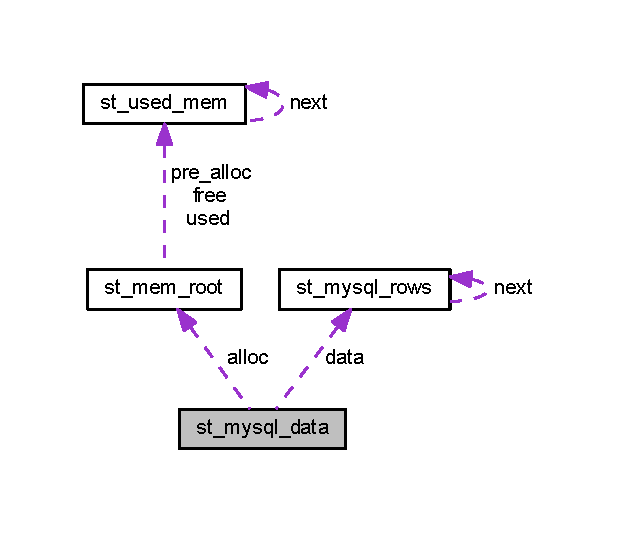
\includegraphics[width=296pt]{structst__mysql__data__coll__graph}
\end{center}
\end{figure}
\subsection*{Data Fields}
\begin{DoxyCompactItemize}
\item 
\hyperlink{mysql_8h_a4d0140764825a51eae874c641df1afb5}{M\+Y\+S\+Q\+L\+\_\+\+R\+O\+W\+S} $\ast$ \hyperlink{structst__mysql__data_a337e8b819b025e698105616e55d76c4a}{data}
\item 
struct embedded\+\_\+query\+\_\+result $\ast$ \hyperlink{structst__mysql__data_ac3e93e741da8215714fbb6e6b6db603b}{embedded\+\_\+info}
\item 
\hyperlink{my__alloc_8h_ac59e289b254a2c5ac634ffcedda3f823}{M\+E\+M\+\_\+\+R\+O\+O\+T} \hyperlink{structst__mysql__data_a177d9effffa87659af590d973ab8d955}{alloc}
\item 
\hyperlink{mysql_8h_ae05bd5d3e5a75578e2f14cfeb43f07aa}{my\+\_\+ulonglong} \hyperlink{structst__mysql__data_ad22f63e6158c6b6e408fdcb255fdbe3d}{rows}
\item 
unsigned int \hyperlink{structst__mysql__data_a2f8ebd2f46566f6476d3588b7e6ea25c}{fields}
\item 
void $\ast$ \hyperlink{structst__mysql__data_afe54e3ced201bd33385957d58520d5a3}{extension}
\end{DoxyCompactItemize}


\subsection{Field Documentation}
\hypertarget{structst__mysql__data_a177d9effffa87659af590d973ab8d955}{}\index{st\+\_\+mysql\+\_\+data@{st\+\_\+mysql\+\_\+data}!alloc@{alloc}}
\index{alloc@{alloc}!st\+\_\+mysql\+\_\+data@{st\+\_\+mysql\+\_\+data}}
\subsubsection[{alloc}]{\setlength{\rightskip}{0pt plus 5cm}{\bf M\+E\+M\+\_\+\+R\+O\+O\+T} st\+\_\+mysql\+\_\+data\+::alloc}\label{structst__mysql__data_a177d9effffa87659af590d973ab8d955}
\hypertarget{structst__mysql__data_a337e8b819b025e698105616e55d76c4a}{}\index{st\+\_\+mysql\+\_\+data@{st\+\_\+mysql\+\_\+data}!data@{data}}
\index{data@{data}!st\+\_\+mysql\+\_\+data@{st\+\_\+mysql\+\_\+data}}
\subsubsection[{data}]{\setlength{\rightskip}{0pt plus 5cm}{\bf M\+Y\+S\+Q\+L\+\_\+\+R\+O\+W\+S}$\ast$ st\+\_\+mysql\+\_\+data\+::data}\label{structst__mysql__data_a337e8b819b025e698105616e55d76c4a}
\hypertarget{structst__mysql__data_ac3e93e741da8215714fbb6e6b6db603b}{}\index{st\+\_\+mysql\+\_\+data@{st\+\_\+mysql\+\_\+data}!embedded\+\_\+info@{embedded\+\_\+info}}
\index{embedded\+\_\+info@{embedded\+\_\+info}!st\+\_\+mysql\+\_\+data@{st\+\_\+mysql\+\_\+data}}
\subsubsection[{embedded\+\_\+info}]{\setlength{\rightskip}{0pt plus 5cm}struct embedded\+\_\+query\+\_\+result$\ast$ st\+\_\+mysql\+\_\+data\+::embedded\+\_\+info}\label{structst__mysql__data_ac3e93e741da8215714fbb6e6b6db603b}
\hypertarget{structst__mysql__data_afe54e3ced201bd33385957d58520d5a3}{}\index{st\+\_\+mysql\+\_\+data@{st\+\_\+mysql\+\_\+data}!extension@{extension}}
\index{extension@{extension}!st\+\_\+mysql\+\_\+data@{st\+\_\+mysql\+\_\+data}}
\subsubsection[{extension}]{\setlength{\rightskip}{0pt plus 5cm}void$\ast$ st\+\_\+mysql\+\_\+data\+::extension}\label{structst__mysql__data_afe54e3ced201bd33385957d58520d5a3}
\hypertarget{structst__mysql__data_a2f8ebd2f46566f6476d3588b7e6ea25c}{}\index{st\+\_\+mysql\+\_\+data@{st\+\_\+mysql\+\_\+data}!fields@{fields}}
\index{fields@{fields}!st\+\_\+mysql\+\_\+data@{st\+\_\+mysql\+\_\+data}}
\subsubsection[{fields}]{\setlength{\rightskip}{0pt plus 5cm}unsigned int st\+\_\+mysql\+\_\+data\+::fields}\label{structst__mysql__data_a2f8ebd2f46566f6476d3588b7e6ea25c}
\hypertarget{structst__mysql__data_ad22f63e6158c6b6e408fdcb255fdbe3d}{}\index{st\+\_\+mysql\+\_\+data@{st\+\_\+mysql\+\_\+data}!rows@{rows}}
\index{rows@{rows}!st\+\_\+mysql\+\_\+data@{st\+\_\+mysql\+\_\+data}}
\subsubsection[{rows}]{\setlength{\rightskip}{0pt plus 5cm}{\bf my\+\_\+ulonglong} st\+\_\+mysql\+\_\+data\+::rows}\label{structst__mysql__data_ad22f63e6158c6b6e408fdcb255fdbe3d}


The documentation for this struct was generated from the following file\+:\begin{DoxyCompactItemize}
\item 
\hyperlink{mysql_8h}{mysql.\+h}\end{DoxyCompactItemize}

\hypertarget{structst__mysql__field}{}\section{st\+\_\+mysql\+\_\+field Struct Reference}
\label{structst__mysql__field}\index{st\+\_\+mysql\+\_\+field@{st\+\_\+mysql\+\_\+field}}


{\ttfamily \#include $<$mysql.\+h$>$}

\subsection*{Data Fields}
\begin{DoxyCompactItemize}
\item 
char $\ast$ \hyperlink{structst__mysql__field_a9aea18cced6a6cd06f9ab3dd75643675}{name}
\item 
char $\ast$ \hyperlink{structst__mysql__field_a03345260f7ab6ff2aab0ee5cda2c8ba3}{org\+\_\+name}
\item 
char $\ast$ \hyperlink{structst__mysql__field_a29e2e9a3a039afd113f5b01144aeadf3}{table}
\item 
char $\ast$ \hyperlink{structst__mysql__field_ade5ec83de3b2537fbffbad382314521f}{org\+\_\+table}
\item 
char $\ast$ \hyperlink{structst__mysql__field_a707bf664b65d46c5fafcc9117d43c3d6}{db}
\item 
char $\ast$ \hyperlink{structst__mysql__field_a5efd1f038fd402730cd69b9b0be93ac6}{catalog}
\item 
char $\ast$ \hyperlink{structst__mysql__field_acd02783a4aa6564a73efd4234043e17b}{def}
\item 
unsigned long \hyperlink{structst__mysql__field_a03ff1a4c1b3d3249d5ff7b1a62f152f3}{length}
\item 
unsigned long \hyperlink{structst__mysql__field_a89db90d875f6b760f147e70ac5f96dce}{max\+\_\+length}
\item 
unsigned int \hyperlink{structst__mysql__field_a9f783bae03537ebb992ca091b7173d92}{name\+\_\+length}
\item 
unsigned int \hyperlink{structst__mysql__field_a76f2446ec6439f82c2d387085498e599}{org\+\_\+name\+\_\+length}
\item 
unsigned int \hyperlink{structst__mysql__field_a3fd823f20119f559007cc41089bec0fe}{table\+\_\+length}
\item 
unsigned int \hyperlink{structst__mysql__field_afa4e4cdb3af1c33edb72757f3fce9e7a}{org\+\_\+table\+\_\+length}
\item 
unsigned int \hyperlink{structst__mysql__field_abe39f84a0bf3580baefe02d1af84b176}{db\+\_\+length}
\item 
unsigned int \hyperlink{structst__mysql__field_a72598be1e648074291e3d8efd1a33d76}{catalog\+\_\+length}
\item 
unsigned int \hyperlink{structst__mysql__field_a6698d0723c7d4349a707fc2bed3641d5}{def\+\_\+length}
\item 
unsigned int \hyperlink{structst__mysql__field_a2977653fe904c10974aeda70fdde5ba2}{flags}
\item 
unsigned int \hyperlink{structst__mysql__field_ab39f6f0fb49ba3ce21522b68f41b4337}{decimals}
\item 
unsigned int \hyperlink{structst__mysql__field_a687f7df1f421ac5273adfc06b244c883}{charsetnr}
\item 
enum \hyperlink{mysql__com_8h_a69e798807026a0f7e12b1d6c72374854}{enum\+\_\+field\+\_\+types} \hyperlink{structst__mysql__field_a3b744bf19e92b619e725b45f83a78771}{type}
\item 
void $\ast$ \hyperlink{structst__mysql__field_a3e03bdbb5de8f5bf461a3591827a3760}{extension}
\end{DoxyCompactItemize}


\subsection{Field Documentation}
\hypertarget{structst__mysql__field_a5efd1f038fd402730cd69b9b0be93ac6}{}\index{st\+\_\+mysql\+\_\+field@{st\+\_\+mysql\+\_\+field}!catalog@{catalog}}
\index{catalog@{catalog}!st\+\_\+mysql\+\_\+field@{st\+\_\+mysql\+\_\+field}}
\subsubsection[{catalog}]{\setlength{\rightskip}{0pt plus 5cm}char$\ast$ st\+\_\+mysql\+\_\+field\+::catalog}\label{structst__mysql__field_a5efd1f038fd402730cd69b9b0be93ac6}
\hypertarget{structst__mysql__field_a72598be1e648074291e3d8efd1a33d76}{}\index{st\+\_\+mysql\+\_\+field@{st\+\_\+mysql\+\_\+field}!catalog\+\_\+length@{catalog\+\_\+length}}
\index{catalog\+\_\+length@{catalog\+\_\+length}!st\+\_\+mysql\+\_\+field@{st\+\_\+mysql\+\_\+field}}
\subsubsection[{catalog\+\_\+length}]{\setlength{\rightskip}{0pt plus 5cm}unsigned int st\+\_\+mysql\+\_\+field\+::catalog\+\_\+length}\label{structst__mysql__field_a72598be1e648074291e3d8efd1a33d76}
\hypertarget{structst__mysql__field_a687f7df1f421ac5273adfc06b244c883}{}\index{st\+\_\+mysql\+\_\+field@{st\+\_\+mysql\+\_\+field}!charsetnr@{charsetnr}}
\index{charsetnr@{charsetnr}!st\+\_\+mysql\+\_\+field@{st\+\_\+mysql\+\_\+field}}
\subsubsection[{charsetnr}]{\setlength{\rightskip}{0pt plus 5cm}unsigned int st\+\_\+mysql\+\_\+field\+::charsetnr}\label{structst__mysql__field_a687f7df1f421ac5273adfc06b244c883}
\hypertarget{structst__mysql__field_a707bf664b65d46c5fafcc9117d43c3d6}{}\index{st\+\_\+mysql\+\_\+field@{st\+\_\+mysql\+\_\+field}!db@{db}}
\index{db@{db}!st\+\_\+mysql\+\_\+field@{st\+\_\+mysql\+\_\+field}}
\subsubsection[{db}]{\setlength{\rightskip}{0pt plus 5cm}char$\ast$ st\+\_\+mysql\+\_\+field\+::db}\label{structst__mysql__field_a707bf664b65d46c5fafcc9117d43c3d6}
\hypertarget{structst__mysql__field_abe39f84a0bf3580baefe02d1af84b176}{}\index{st\+\_\+mysql\+\_\+field@{st\+\_\+mysql\+\_\+field}!db\+\_\+length@{db\+\_\+length}}
\index{db\+\_\+length@{db\+\_\+length}!st\+\_\+mysql\+\_\+field@{st\+\_\+mysql\+\_\+field}}
\subsubsection[{db\+\_\+length}]{\setlength{\rightskip}{0pt plus 5cm}unsigned int st\+\_\+mysql\+\_\+field\+::db\+\_\+length}\label{structst__mysql__field_abe39f84a0bf3580baefe02d1af84b176}
\hypertarget{structst__mysql__field_ab39f6f0fb49ba3ce21522b68f41b4337}{}\index{st\+\_\+mysql\+\_\+field@{st\+\_\+mysql\+\_\+field}!decimals@{decimals}}
\index{decimals@{decimals}!st\+\_\+mysql\+\_\+field@{st\+\_\+mysql\+\_\+field}}
\subsubsection[{decimals}]{\setlength{\rightskip}{0pt plus 5cm}unsigned int st\+\_\+mysql\+\_\+field\+::decimals}\label{structst__mysql__field_ab39f6f0fb49ba3ce21522b68f41b4337}
\hypertarget{structst__mysql__field_acd02783a4aa6564a73efd4234043e17b}{}\index{st\+\_\+mysql\+\_\+field@{st\+\_\+mysql\+\_\+field}!def@{def}}
\index{def@{def}!st\+\_\+mysql\+\_\+field@{st\+\_\+mysql\+\_\+field}}
\subsubsection[{def}]{\setlength{\rightskip}{0pt plus 5cm}char$\ast$ st\+\_\+mysql\+\_\+field\+::def}\label{structst__mysql__field_acd02783a4aa6564a73efd4234043e17b}
\hypertarget{structst__mysql__field_a6698d0723c7d4349a707fc2bed3641d5}{}\index{st\+\_\+mysql\+\_\+field@{st\+\_\+mysql\+\_\+field}!def\+\_\+length@{def\+\_\+length}}
\index{def\+\_\+length@{def\+\_\+length}!st\+\_\+mysql\+\_\+field@{st\+\_\+mysql\+\_\+field}}
\subsubsection[{def\+\_\+length}]{\setlength{\rightskip}{0pt plus 5cm}unsigned int st\+\_\+mysql\+\_\+field\+::def\+\_\+length}\label{structst__mysql__field_a6698d0723c7d4349a707fc2bed3641d5}
\hypertarget{structst__mysql__field_a3e03bdbb5de8f5bf461a3591827a3760}{}\index{st\+\_\+mysql\+\_\+field@{st\+\_\+mysql\+\_\+field}!extension@{extension}}
\index{extension@{extension}!st\+\_\+mysql\+\_\+field@{st\+\_\+mysql\+\_\+field}}
\subsubsection[{extension}]{\setlength{\rightskip}{0pt plus 5cm}void$\ast$ st\+\_\+mysql\+\_\+field\+::extension}\label{structst__mysql__field_a3e03bdbb5de8f5bf461a3591827a3760}
\hypertarget{structst__mysql__field_a2977653fe904c10974aeda70fdde5ba2}{}\index{st\+\_\+mysql\+\_\+field@{st\+\_\+mysql\+\_\+field}!flags@{flags}}
\index{flags@{flags}!st\+\_\+mysql\+\_\+field@{st\+\_\+mysql\+\_\+field}}
\subsubsection[{flags}]{\setlength{\rightskip}{0pt plus 5cm}unsigned int st\+\_\+mysql\+\_\+field\+::flags}\label{structst__mysql__field_a2977653fe904c10974aeda70fdde5ba2}
\hypertarget{structst__mysql__field_a03ff1a4c1b3d3249d5ff7b1a62f152f3}{}\index{st\+\_\+mysql\+\_\+field@{st\+\_\+mysql\+\_\+field}!length@{length}}
\index{length@{length}!st\+\_\+mysql\+\_\+field@{st\+\_\+mysql\+\_\+field}}
\subsubsection[{length}]{\setlength{\rightskip}{0pt plus 5cm}unsigned long st\+\_\+mysql\+\_\+field\+::length}\label{structst__mysql__field_a03ff1a4c1b3d3249d5ff7b1a62f152f3}
\hypertarget{structst__mysql__field_a89db90d875f6b760f147e70ac5f96dce}{}\index{st\+\_\+mysql\+\_\+field@{st\+\_\+mysql\+\_\+field}!max\+\_\+length@{max\+\_\+length}}
\index{max\+\_\+length@{max\+\_\+length}!st\+\_\+mysql\+\_\+field@{st\+\_\+mysql\+\_\+field}}
\subsubsection[{max\+\_\+length}]{\setlength{\rightskip}{0pt plus 5cm}unsigned long st\+\_\+mysql\+\_\+field\+::max\+\_\+length}\label{structst__mysql__field_a89db90d875f6b760f147e70ac5f96dce}
\hypertarget{structst__mysql__field_a9aea18cced6a6cd06f9ab3dd75643675}{}\index{st\+\_\+mysql\+\_\+field@{st\+\_\+mysql\+\_\+field}!name@{name}}
\index{name@{name}!st\+\_\+mysql\+\_\+field@{st\+\_\+mysql\+\_\+field}}
\subsubsection[{name}]{\setlength{\rightskip}{0pt plus 5cm}char$\ast$ st\+\_\+mysql\+\_\+field\+::name}\label{structst__mysql__field_a9aea18cced6a6cd06f9ab3dd75643675}
\hypertarget{structst__mysql__field_a9f783bae03537ebb992ca091b7173d92}{}\index{st\+\_\+mysql\+\_\+field@{st\+\_\+mysql\+\_\+field}!name\+\_\+length@{name\+\_\+length}}
\index{name\+\_\+length@{name\+\_\+length}!st\+\_\+mysql\+\_\+field@{st\+\_\+mysql\+\_\+field}}
\subsubsection[{name\+\_\+length}]{\setlength{\rightskip}{0pt plus 5cm}unsigned int st\+\_\+mysql\+\_\+field\+::name\+\_\+length}\label{structst__mysql__field_a9f783bae03537ebb992ca091b7173d92}
\hypertarget{structst__mysql__field_a03345260f7ab6ff2aab0ee5cda2c8ba3}{}\index{st\+\_\+mysql\+\_\+field@{st\+\_\+mysql\+\_\+field}!org\+\_\+name@{org\+\_\+name}}
\index{org\+\_\+name@{org\+\_\+name}!st\+\_\+mysql\+\_\+field@{st\+\_\+mysql\+\_\+field}}
\subsubsection[{org\+\_\+name}]{\setlength{\rightskip}{0pt plus 5cm}char$\ast$ st\+\_\+mysql\+\_\+field\+::org\+\_\+name}\label{structst__mysql__field_a03345260f7ab6ff2aab0ee5cda2c8ba3}
\hypertarget{structst__mysql__field_a76f2446ec6439f82c2d387085498e599}{}\index{st\+\_\+mysql\+\_\+field@{st\+\_\+mysql\+\_\+field}!org\+\_\+name\+\_\+length@{org\+\_\+name\+\_\+length}}
\index{org\+\_\+name\+\_\+length@{org\+\_\+name\+\_\+length}!st\+\_\+mysql\+\_\+field@{st\+\_\+mysql\+\_\+field}}
\subsubsection[{org\+\_\+name\+\_\+length}]{\setlength{\rightskip}{0pt plus 5cm}unsigned int st\+\_\+mysql\+\_\+field\+::org\+\_\+name\+\_\+length}\label{structst__mysql__field_a76f2446ec6439f82c2d387085498e599}
\hypertarget{structst__mysql__field_ade5ec83de3b2537fbffbad382314521f}{}\index{st\+\_\+mysql\+\_\+field@{st\+\_\+mysql\+\_\+field}!org\+\_\+table@{org\+\_\+table}}
\index{org\+\_\+table@{org\+\_\+table}!st\+\_\+mysql\+\_\+field@{st\+\_\+mysql\+\_\+field}}
\subsubsection[{org\+\_\+table}]{\setlength{\rightskip}{0pt plus 5cm}char$\ast$ st\+\_\+mysql\+\_\+field\+::org\+\_\+table}\label{structst__mysql__field_ade5ec83de3b2537fbffbad382314521f}
\hypertarget{structst__mysql__field_afa4e4cdb3af1c33edb72757f3fce9e7a}{}\index{st\+\_\+mysql\+\_\+field@{st\+\_\+mysql\+\_\+field}!org\+\_\+table\+\_\+length@{org\+\_\+table\+\_\+length}}
\index{org\+\_\+table\+\_\+length@{org\+\_\+table\+\_\+length}!st\+\_\+mysql\+\_\+field@{st\+\_\+mysql\+\_\+field}}
\subsubsection[{org\+\_\+table\+\_\+length}]{\setlength{\rightskip}{0pt plus 5cm}unsigned int st\+\_\+mysql\+\_\+field\+::org\+\_\+table\+\_\+length}\label{structst__mysql__field_afa4e4cdb3af1c33edb72757f3fce9e7a}
\hypertarget{structst__mysql__field_a29e2e9a3a039afd113f5b01144aeadf3}{}\index{st\+\_\+mysql\+\_\+field@{st\+\_\+mysql\+\_\+field}!table@{table}}
\index{table@{table}!st\+\_\+mysql\+\_\+field@{st\+\_\+mysql\+\_\+field}}
\subsubsection[{table}]{\setlength{\rightskip}{0pt plus 5cm}char$\ast$ st\+\_\+mysql\+\_\+field\+::table}\label{structst__mysql__field_a29e2e9a3a039afd113f5b01144aeadf3}
\hypertarget{structst__mysql__field_a3fd823f20119f559007cc41089bec0fe}{}\index{st\+\_\+mysql\+\_\+field@{st\+\_\+mysql\+\_\+field}!table\+\_\+length@{table\+\_\+length}}
\index{table\+\_\+length@{table\+\_\+length}!st\+\_\+mysql\+\_\+field@{st\+\_\+mysql\+\_\+field}}
\subsubsection[{table\+\_\+length}]{\setlength{\rightskip}{0pt plus 5cm}unsigned int st\+\_\+mysql\+\_\+field\+::table\+\_\+length}\label{structst__mysql__field_a3fd823f20119f559007cc41089bec0fe}
\hypertarget{structst__mysql__field_a3b744bf19e92b619e725b45f83a78771}{}\index{st\+\_\+mysql\+\_\+field@{st\+\_\+mysql\+\_\+field}!type@{type}}
\index{type@{type}!st\+\_\+mysql\+\_\+field@{st\+\_\+mysql\+\_\+field}}
\subsubsection[{type}]{\setlength{\rightskip}{0pt plus 5cm}enum {\bf enum\+\_\+field\+\_\+types} st\+\_\+mysql\+\_\+field\+::type}\label{structst__mysql__field_a3b744bf19e92b619e725b45f83a78771}


The documentation for this struct was generated from the following file\+:\begin{DoxyCompactItemize}
\item 
\hyperlink{mysql_8h}{mysql.\+h}\end{DoxyCompactItemize}

\hypertarget{structst__mysql__options}{}\section{st\+\_\+mysql\+\_\+options Struct Reference}
\label{structst__mysql__options}\index{st\+\_\+mysql\+\_\+options@{st\+\_\+mysql\+\_\+options}}


{\ttfamily \#include $<$mysql.\+h$>$}

\subsection*{Data Fields}
\begin{DoxyCompactItemize}
\item 
unsigned int \hyperlink{structst__mysql__options_aa8475fa207a033461041fbfd868fe3c6}{connect\+\_\+timeout}
\item 
unsigned int \hyperlink{structst__mysql__options_a6fbcc8e03aa4c489bfa23de7f4e0d8f8}{read\+\_\+timeout}
\item 
unsigned int \hyperlink{structst__mysql__options_a8956fca97f0263e415546f5624a614d2}{write\+\_\+timeout}
\item 
unsigned int \hyperlink{structst__mysql__options_a1403738b86df8bc7056a33b50bd8aff5}{port}
\item 
unsigned int \hyperlink{structst__mysql__options_a85283d4471c23b3773ca0c4c01ffb1f7}{protocol}
\item 
unsigned long \hyperlink{structst__mysql__options_a92c47dfe1c8de03a65b81863a88c9355}{client\+\_\+flag}
\item 
char $\ast$ \hyperlink{structst__mysql__options_a79fc433d16a9cd4b913a6490fc612bf3}{host}
\item 
char $\ast$ \hyperlink{structst__mysql__options_a9889ada2bcc6e077b8ee984a9c7be6e1}{user}
\item 
char $\ast$ \hyperlink{structst__mysql__options_a76f9c11ae054459cabfc89d30928b786}{password}
\item 
char $\ast$ \hyperlink{structst__mysql__options_a6d4f1507ec3907eda109548da49ee850}{unix\+\_\+socket}
\item 
char $\ast$ \hyperlink{structst__mysql__options_a82f5dcf8b83007fafa33a45583f87ce8}{db}
\item 
struct st\+\_\+dynamic\+\_\+array $\ast$ \hyperlink{structst__mysql__options_a6f9eb2e4acb59618e0843bb3c63f58f4}{init\+\_\+commands}
\item 
char $\ast$ \hyperlink{structst__mysql__options_a4cc1dad4e2d110efa24865a636613b6e}{my\+\_\+cnf\+\_\+file}
\item 
char $\ast$ \hyperlink{structst__mysql__options_a28e998c549cbbc33d7d1eba197f1d52f}{my\+\_\+cnf\+\_\+group}
\item 
char $\ast$ \hyperlink{structst__mysql__options_a8e4ad7ebde4a8956788247faf4da20fb}{charset\+\_\+dir}
\item 
char $\ast$ \hyperlink{structst__mysql__options_a965be4c3b508a911b575fc0aa8fc3345}{charset\+\_\+name}
\item 
char $\ast$ \hyperlink{structst__mysql__options_a43176d9b1d3e5e54ac0b2c263ec4441a}{ssl\+\_\+key}
\item 
char $\ast$ \hyperlink{structst__mysql__options_a4723de8759d3e167f5690fe2abfb98a9}{ssl\+\_\+cert}
\item 
char $\ast$ \hyperlink{structst__mysql__options_a418b114edbc344a140c90df9d1f2cd39}{ssl\+\_\+ca}
\item 
char $\ast$ \hyperlink{structst__mysql__options_a19477c3410299535e086c5fe482f06f4}{ssl\+\_\+capath}
\item 
char $\ast$ \hyperlink{structst__mysql__options_a79dd7a4b9bec6d8d6fb17027dcc49c9e}{ssl\+\_\+cipher}
\item 
char $\ast$ \hyperlink{structst__mysql__options_abd61d3820e3904dd30ad1c4c44887d10}{shared\+\_\+memory\+\_\+base\+\_\+name}
\item 
unsigned long \hyperlink{structst__mysql__options_a70de1a0467629fc3ccb1b0c12431fb41}{max\+\_\+allowed\+\_\+packet}
\item 
\hyperlink{mysql_8h_a74cd599039dcf29c6e6d342cf4efd0a8}{my\+\_\+bool} \hyperlink{structst__mysql__options_a4c429488249a27b52cbd3757e15c17c9}{use\+\_\+ssl}
\item 
\hyperlink{mysql_8h_a74cd599039dcf29c6e6d342cf4efd0a8}{my\+\_\+bool} \hyperlink{structst__mysql__options_ab142434a4e128b82feeebbe6e2dd5e00}{compress}
\item 
\hyperlink{mysql_8h_a74cd599039dcf29c6e6d342cf4efd0a8}{my\+\_\+bool} \hyperlink{structst__mysql__options_ab653028194e8666e5d7d16194f88675e}{named\+\_\+pipe}
\item 
\hyperlink{mysql_8h_a74cd599039dcf29c6e6d342cf4efd0a8}{my\+\_\+bool} \hyperlink{structst__mysql__options_aba1f9319c86456a855b662ae4b8de31a}{unused1}
\item 
\hyperlink{mysql_8h_a74cd599039dcf29c6e6d342cf4efd0a8}{my\+\_\+bool} \hyperlink{structst__mysql__options_addcd685e426bca0f3aca8dbbe1ffe427}{unused2}
\item 
\hyperlink{mysql_8h_a74cd599039dcf29c6e6d342cf4efd0a8}{my\+\_\+bool} \hyperlink{structst__mysql__options_a961daa92001900751dd15073e7dcfb21}{unused3}
\item 
\hyperlink{mysql_8h_a74cd599039dcf29c6e6d342cf4efd0a8}{my\+\_\+bool} \hyperlink{structst__mysql__options_a23ea8e676bc687b865b5842254e88e6d}{unused4}
\item 
enum \hyperlink{mysql_8h_a255d4e9a14d73dde30125232fefac836}{mysql\+\_\+option} \hyperlink{structst__mysql__options_a76fecd9908ce3203903d987e4b3c5599}{methods\+\_\+to\+\_\+use}
\item 
\begin{tabbing}
xx\=xx\=xx\=xx\=xx\=xx\=xx\=xx\=xx\=\kill
union \{\\
\>char $\ast$ \hyperlink{structst__mysql__options_a303edbbc594a8ccbfa3de34aa85ae509}{client\_ip}\\
\>char $\ast$ \hyperlink{structst__mysql__options_a91d2448d2fd587a02752f34e64f9680d}{bind\_address}\\
\} \hyperlink{structst__mysql__options_a9ffe17c90b136c23df2cabd2e0eac835}{ci}\\

\end{tabbing}\item 
\hyperlink{mysql_8h_a74cd599039dcf29c6e6d342cf4efd0a8}{my\+\_\+bool} \hyperlink{structst__mysql__options_a6a2e197dd368bd0c110ab2e962369abd}{unused5}
\item 
\hyperlink{mysql_8h_a74cd599039dcf29c6e6d342cf4efd0a8}{my\+\_\+bool} \hyperlink{structst__mysql__options_a095ec6fb5b58914a518522376a0d49ba}{report\+\_\+data\+\_\+truncation}
\item 
int($\ast$ \hyperlink{structst__mysql__options_a3524e3b6573ae25e1b3f26b19d818f10}{local\+\_\+infile\+\_\+init} )(void $\ast$$\ast$, const char $\ast$, void $\ast$)
\item 
int($\ast$ \hyperlink{structst__mysql__options_adff315c42cebf0390d3d14f1bee762bc}{local\+\_\+infile\+\_\+read} )(void $\ast$, char $\ast$, unsigned int)
\item 
void($\ast$ \hyperlink{structst__mysql__options_a45658a7c3298bbd90e9dc61cee282f05}{local\+\_\+infile\+\_\+end} )(void $\ast$)
\item 
int($\ast$ \hyperlink{structst__mysql__options_a79b831a574398e1ba37f0c7052318269}{local\+\_\+infile\+\_\+error} )(void $\ast$, char $\ast$, unsigned int)
\item 
void $\ast$ \hyperlink{structst__mysql__options_a54cbdc47b238a839eff42269b871380d}{local\+\_\+infile\+\_\+userdata}
\item 
struct st\+\_\+mysql\+\_\+options\+\_\+extention $\ast$ \hyperlink{structst__mysql__options_ac16c1d9c8c28b3daeabb7222cda5e8c2}{extension}
\end{DoxyCompactItemize}


\subsection{Field Documentation}
\hypertarget{structst__mysql__options_a91d2448d2fd587a02752f34e64f9680d}{}\index{st\+\_\+mysql\+\_\+options@{st\+\_\+mysql\+\_\+options}!bind\+\_\+address@{bind\+\_\+address}}
\index{bind\+\_\+address@{bind\+\_\+address}!st\+\_\+mysql\+\_\+options@{st\+\_\+mysql\+\_\+options}}
\subsubsection[{bind\+\_\+address}]{\setlength{\rightskip}{0pt plus 5cm}char$\ast$ st\+\_\+mysql\+\_\+options\+::bind\+\_\+address}\label{structst__mysql__options_a91d2448d2fd587a02752f34e64f9680d}
\hypertarget{structst__mysql__options_a8e4ad7ebde4a8956788247faf4da20fb}{}\index{st\+\_\+mysql\+\_\+options@{st\+\_\+mysql\+\_\+options}!charset\+\_\+dir@{charset\+\_\+dir}}
\index{charset\+\_\+dir@{charset\+\_\+dir}!st\+\_\+mysql\+\_\+options@{st\+\_\+mysql\+\_\+options}}
\subsubsection[{charset\+\_\+dir}]{\setlength{\rightskip}{0pt plus 5cm}char $\ast$ st\+\_\+mysql\+\_\+options\+::charset\+\_\+dir}\label{structst__mysql__options_a8e4ad7ebde4a8956788247faf4da20fb}
\hypertarget{structst__mysql__options_a965be4c3b508a911b575fc0aa8fc3345}{}\index{st\+\_\+mysql\+\_\+options@{st\+\_\+mysql\+\_\+options}!charset\+\_\+name@{charset\+\_\+name}}
\index{charset\+\_\+name@{charset\+\_\+name}!st\+\_\+mysql\+\_\+options@{st\+\_\+mysql\+\_\+options}}
\subsubsection[{charset\+\_\+name}]{\setlength{\rightskip}{0pt plus 5cm}char $\ast$ st\+\_\+mysql\+\_\+options\+::charset\+\_\+name}\label{structst__mysql__options_a965be4c3b508a911b575fc0aa8fc3345}
\hypertarget{structst__mysql__options_a9ffe17c90b136c23df2cabd2e0eac835}{}\index{st\+\_\+mysql\+\_\+options@{st\+\_\+mysql\+\_\+options}!ci@{ci}}
\index{ci@{ci}!st\+\_\+mysql\+\_\+options@{st\+\_\+mysql\+\_\+options}}
\subsubsection[{ci}]{\setlength{\rightskip}{0pt plus 5cm}union \{ ... \}   st\+\_\+mysql\+\_\+options\+::ci}\label{structst__mysql__options_a9ffe17c90b136c23df2cabd2e0eac835}
\hypertarget{structst__mysql__options_a92c47dfe1c8de03a65b81863a88c9355}{}\index{st\+\_\+mysql\+\_\+options@{st\+\_\+mysql\+\_\+options}!client\+\_\+flag@{client\+\_\+flag}}
\index{client\+\_\+flag@{client\+\_\+flag}!st\+\_\+mysql\+\_\+options@{st\+\_\+mysql\+\_\+options}}
\subsubsection[{client\+\_\+flag}]{\setlength{\rightskip}{0pt plus 5cm}unsigned long st\+\_\+mysql\+\_\+options\+::client\+\_\+flag}\label{structst__mysql__options_a92c47dfe1c8de03a65b81863a88c9355}
\hypertarget{structst__mysql__options_a303edbbc594a8ccbfa3de34aa85ae509}{}\index{st\+\_\+mysql\+\_\+options@{st\+\_\+mysql\+\_\+options}!client\+\_\+ip@{client\+\_\+ip}}
\index{client\+\_\+ip@{client\+\_\+ip}!st\+\_\+mysql\+\_\+options@{st\+\_\+mysql\+\_\+options}}
\subsubsection[{client\+\_\+ip}]{\setlength{\rightskip}{0pt plus 5cm}char$\ast$ st\+\_\+mysql\+\_\+options\+::client\+\_\+ip}\label{structst__mysql__options_a303edbbc594a8ccbfa3de34aa85ae509}
\hypertarget{structst__mysql__options_ab142434a4e128b82feeebbe6e2dd5e00}{}\index{st\+\_\+mysql\+\_\+options@{st\+\_\+mysql\+\_\+options}!compress@{compress}}
\index{compress@{compress}!st\+\_\+mysql\+\_\+options@{st\+\_\+mysql\+\_\+options}}
\subsubsection[{compress}]{\setlength{\rightskip}{0pt plus 5cm}{\bf my\+\_\+bool} st\+\_\+mysql\+\_\+options\+::compress}\label{structst__mysql__options_ab142434a4e128b82feeebbe6e2dd5e00}
\hypertarget{structst__mysql__options_aa8475fa207a033461041fbfd868fe3c6}{}\index{st\+\_\+mysql\+\_\+options@{st\+\_\+mysql\+\_\+options}!connect\+\_\+timeout@{connect\+\_\+timeout}}
\index{connect\+\_\+timeout@{connect\+\_\+timeout}!st\+\_\+mysql\+\_\+options@{st\+\_\+mysql\+\_\+options}}
\subsubsection[{connect\+\_\+timeout}]{\setlength{\rightskip}{0pt plus 5cm}unsigned int st\+\_\+mysql\+\_\+options\+::connect\+\_\+timeout}\label{structst__mysql__options_aa8475fa207a033461041fbfd868fe3c6}
\hypertarget{structst__mysql__options_a82f5dcf8b83007fafa33a45583f87ce8}{}\index{st\+\_\+mysql\+\_\+options@{st\+\_\+mysql\+\_\+options}!db@{db}}
\index{db@{db}!st\+\_\+mysql\+\_\+options@{st\+\_\+mysql\+\_\+options}}
\subsubsection[{db}]{\setlength{\rightskip}{0pt plus 5cm}char $\ast$ st\+\_\+mysql\+\_\+options\+::db}\label{structst__mysql__options_a82f5dcf8b83007fafa33a45583f87ce8}
\hypertarget{structst__mysql__options_ac16c1d9c8c28b3daeabb7222cda5e8c2}{}\index{st\+\_\+mysql\+\_\+options@{st\+\_\+mysql\+\_\+options}!extension@{extension}}
\index{extension@{extension}!st\+\_\+mysql\+\_\+options@{st\+\_\+mysql\+\_\+options}}
\subsubsection[{extension}]{\setlength{\rightskip}{0pt plus 5cm}struct st\+\_\+mysql\+\_\+options\+\_\+extention$\ast$ st\+\_\+mysql\+\_\+options\+::extension}\label{structst__mysql__options_ac16c1d9c8c28b3daeabb7222cda5e8c2}
\hypertarget{structst__mysql__options_a79fc433d16a9cd4b913a6490fc612bf3}{}\index{st\+\_\+mysql\+\_\+options@{st\+\_\+mysql\+\_\+options}!host@{host}}
\index{host@{host}!st\+\_\+mysql\+\_\+options@{st\+\_\+mysql\+\_\+options}}
\subsubsection[{host}]{\setlength{\rightskip}{0pt plus 5cm}char$\ast$ st\+\_\+mysql\+\_\+options\+::host}\label{structst__mysql__options_a79fc433d16a9cd4b913a6490fc612bf3}
\hypertarget{structst__mysql__options_a6f9eb2e4acb59618e0843bb3c63f58f4}{}\index{st\+\_\+mysql\+\_\+options@{st\+\_\+mysql\+\_\+options}!init\+\_\+commands@{init\+\_\+commands}}
\index{init\+\_\+commands@{init\+\_\+commands}!st\+\_\+mysql\+\_\+options@{st\+\_\+mysql\+\_\+options}}
\subsubsection[{init\+\_\+commands}]{\setlength{\rightskip}{0pt plus 5cm}struct st\+\_\+dynamic\+\_\+array$\ast$ st\+\_\+mysql\+\_\+options\+::init\+\_\+commands}\label{structst__mysql__options_a6f9eb2e4acb59618e0843bb3c63f58f4}
\hypertarget{structst__mysql__options_a45658a7c3298bbd90e9dc61cee282f05}{}\index{st\+\_\+mysql\+\_\+options@{st\+\_\+mysql\+\_\+options}!local\+\_\+infile\+\_\+end@{local\+\_\+infile\+\_\+end}}
\index{local\+\_\+infile\+\_\+end@{local\+\_\+infile\+\_\+end}!st\+\_\+mysql\+\_\+options@{st\+\_\+mysql\+\_\+options}}
\subsubsection[{local\+\_\+infile\+\_\+end}]{\setlength{\rightskip}{0pt plus 5cm}void($\ast$ st\+\_\+mysql\+\_\+options\+::local\+\_\+infile\+\_\+end) (void $\ast$)}\label{structst__mysql__options_a45658a7c3298bbd90e9dc61cee282f05}
\hypertarget{structst__mysql__options_a79b831a574398e1ba37f0c7052318269}{}\index{st\+\_\+mysql\+\_\+options@{st\+\_\+mysql\+\_\+options}!local\+\_\+infile\+\_\+error@{local\+\_\+infile\+\_\+error}}
\index{local\+\_\+infile\+\_\+error@{local\+\_\+infile\+\_\+error}!st\+\_\+mysql\+\_\+options@{st\+\_\+mysql\+\_\+options}}
\subsubsection[{local\+\_\+infile\+\_\+error}]{\setlength{\rightskip}{0pt plus 5cm}int($\ast$ st\+\_\+mysql\+\_\+options\+::local\+\_\+infile\+\_\+error) (void $\ast$, char $\ast$, unsigned int)}\label{structst__mysql__options_a79b831a574398e1ba37f0c7052318269}
\hypertarget{structst__mysql__options_a3524e3b6573ae25e1b3f26b19d818f10}{}\index{st\+\_\+mysql\+\_\+options@{st\+\_\+mysql\+\_\+options}!local\+\_\+infile\+\_\+init@{local\+\_\+infile\+\_\+init}}
\index{local\+\_\+infile\+\_\+init@{local\+\_\+infile\+\_\+init}!st\+\_\+mysql\+\_\+options@{st\+\_\+mysql\+\_\+options}}
\subsubsection[{local\+\_\+infile\+\_\+init}]{\setlength{\rightskip}{0pt plus 5cm}int($\ast$ st\+\_\+mysql\+\_\+options\+::local\+\_\+infile\+\_\+init) (void $\ast$$\ast$, const char $\ast$, void $\ast$)}\label{structst__mysql__options_a3524e3b6573ae25e1b3f26b19d818f10}
\hypertarget{structst__mysql__options_adff315c42cebf0390d3d14f1bee762bc}{}\index{st\+\_\+mysql\+\_\+options@{st\+\_\+mysql\+\_\+options}!local\+\_\+infile\+\_\+read@{local\+\_\+infile\+\_\+read}}
\index{local\+\_\+infile\+\_\+read@{local\+\_\+infile\+\_\+read}!st\+\_\+mysql\+\_\+options@{st\+\_\+mysql\+\_\+options}}
\subsubsection[{local\+\_\+infile\+\_\+read}]{\setlength{\rightskip}{0pt plus 5cm}int($\ast$ st\+\_\+mysql\+\_\+options\+::local\+\_\+infile\+\_\+read) (void $\ast$, char $\ast$, unsigned int)}\label{structst__mysql__options_adff315c42cebf0390d3d14f1bee762bc}
\hypertarget{structst__mysql__options_a54cbdc47b238a839eff42269b871380d}{}\index{st\+\_\+mysql\+\_\+options@{st\+\_\+mysql\+\_\+options}!local\+\_\+infile\+\_\+userdata@{local\+\_\+infile\+\_\+userdata}}
\index{local\+\_\+infile\+\_\+userdata@{local\+\_\+infile\+\_\+userdata}!st\+\_\+mysql\+\_\+options@{st\+\_\+mysql\+\_\+options}}
\subsubsection[{local\+\_\+infile\+\_\+userdata}]{\setlength{\rightskip}{0pt plus 5cm}void$\ast$ st\+\_\+mysql\+\_\+options\+::local\+\_\+infile\+\_\+userdata}\label{structst__mysql__options_a54cbdc47b238a839eff42269b871380d}
\hypertarget{structst__mysql__options_a70de1a0467629fc3ccb1b0c12431fb41}{}\index{st\+\_\+mysql\+\_\+options@{st\+\_\+mysql\+\_\+options}!max\+\_\+allowed\+\_\+packet@{max\+\_\+allowed\+\_\+packet}}
\index{max\+\_\+allowed\+\_\+packet@{max\+\_\+allowed\+\_\+packet}!st\+\_\+mysql\+\_\+options@{st\+\_\+mysql\+\_\+options}}
\subsubsection[{max\+\_\+allowed\+\_\+packet}]{\setlength{\rightskip}{0pt plus 5cm}unsigned long st\+\_\+mysql\+\_\+options\+::max\+\_\+allowed\+\_\+packet}\label{structst__mysql__options_a70de1a0467629fc3ccb1b0c12431fb41}
\hypertarget{structst__mysql__options_a76fecd9908ce3203903d987e4b3c5599}{}\index{st\+\_\+mysql\+\_\+options@{st\+\_\+mysql\+\_\+options}!methods\+\_\+to\+\_\+use@{methods\+\_\+to\+\_\+use}}
\index{methods\+\_\+to\+\_\+use@{methods\+\_\+to\+\_\+use}!st\+\_\+mysql\+\_\+options@{st\+\_\+mysql\+\_\+options}}
\subsubsection[{methods\+\_\+to\+\_\+use}]{\setlength{\rightskip}{0pt plus 5cm}enum {\bf mysql\+\_\+option} st\+\_\+mysql\+\_\+options\+::methods\+\_\+to\+\_\+use}\label{structst__mysql__options_a76fecd9908ce3203903d987e4b3c5599}
\hypertarget{structst__mysql__options_a4cc1dad4e2d110efa24865a636613b6e}{}\index{st\+\_\+mysql\+\_\+options@{st\+\_\+mysql\+\_\+options}!my\+\_\+cnf\+\_\+file@{my\+\_\+cnf\+\_\+file}}
\index{my\+\_\+cnf\+\_\+file@{my\+\_\+cnf\+\_\+file}!st\+\_\+mysql\+\_\+options@{st\+\_\+mysql\+\_\+options}}
\subsubsection[{my\+\_\+cnf\+\_\+file}]{\setlength{\rightskip}{0pt plus 5cm}char$\ast$ st\+\_\+mysql\+\_\+options\+::my\+\_\+cnf\+\_\+file}\label{structst__mysql__options_a4cc1dad4e2d110efa24865a636613b6e}
\hypertarget{structst__mysql__options_a28e998c549cbbc33d7d1eba197f1d52f}{}\index{st\+\_\+mysql\+\_\+options@{st\+\_\+mysql\+\_\+options}!my\+\_\+cnf\+\_\+group@{my\+\_\+cnf\+\_\+group}}
\index{my\+\_\+cnf\+\_\+group@{my\+\_\+cnf\+\_\+group}!st\+\_\+mysql\+\_\+options@{st\+\_\+mysql\+\_\+options}}
\subsubsection[{my\+\_\+cnf\+\_\+group}]{\setlength{\rightskip}{0pt plus 5cm}char $\ast$ st\+\_\+mysql\+\_\+options\+::my\+\_\+cnf\+\_\+group}\label{structst__mysql__options_a28e998c549cbbc33d7d1eba197f1d52f}
\hypertarget{structst__mysql__options_ab653028194e8666e5d7d16194f88675e}{}\index{st\+\_\+mysql\+\_\+options@{st\+\_\+mysql\+\_\+options}!named\+\_\+pipe@{named\+\_\+pipe}}
\index{named\+\_\+pipe@{named\+\_\+pipe}!st\+\_\+mysql\+\_\+options@{st\+\_\+mysql\+\_\+options}}
\subsubsection[{named\+\_\+pipe}]{\setlength{\rightskip}{0pt plus 5cm}{\bf my\+\_\+bool} st\+\_\+mysql\+\_\+options\+::named\+\_\+pipe}\label{structst__mysql__options_ab653028194e8666e5d7d16194f88675e}
\hypertarget{structst__mysql__options_a76f9c11ae054459cabfc89d30928b786}{}\index{st\+\_\+mysql\+\_\+options@{st\+\_\+mysql\+\_\+options}!password@{password}}
\index{password@{password}!st\+\_\+mysql\+\_\+options@{st\+\_\+mysql\+\_\+options}}
\subsubsection[{password}]{\setlength{\rightskip}{0pt plus 5cm}char $\ast$ st\+\_\+mysql\+\_\+options\+::password}\label{structst__mysql__options_a76f9c11ae054459cabfc89d30928b786}
\hypertarget{structst__mysql__options_a1403738b86df8bc7056a33b50bd8aff5}{}\index{st\+\_\+mysql\+\_\+options@{st\+\_\+mysql\+\_\+options}!port@{port}}
\index{port@{port}!st\+\_\+mysql\+\_\+options@{st\+\_\+mysql\+\_\+options}}
\subsubsection[{port}]{\setlength{\rightskip}{0pt plus 5cm}unsigned int st\+\_\+mysql\+\_\+options\+::port}\label{structst__mysql__options_a1403738b86df8bc7056a33b50bd8aff5}
\hypertarget{structst__mysql__options_a85283d4471c23b3773ca0c4c01ffb1f7}{}\index{st\+\_\+mysql\+\_\+options@{st\+\_\+mysql\+\_\+options}!protocol@{protocol}}
\index{protocol@{protocol}!st\+\_\+mysql\+\_\+options@{st\+\_\+mysql\+\_\+options}}
\subsubsection[{protocol}]{\setlength{\rightskip}{0pt plus 5cm}unsigned int st\+\_\+mysql\+\_\+options\+::protocol}\label{structst__mysql__options_a85283d4471c23b3773ca0c4c01ffb1f7}
\hypertarget{structst__mysql__options_a6fbcc8e03aa4c489bfa23de7f4e0d8f8}{}\index{st\+\_\+mysql\+\_\+options@{st\+\_\+mysql\+\_\+options}!read\+\_\+timeout@{read\+\_\+timeout}}
\index{read\+\_\+timeout@{read\+\_\+timeout}!st\+\_\+mysql\+\_\+options@{st\+\_\+mysql\+\_\+options}}
\subsubsection[{read\+\_\+timeout}]{\setlength{\rightskip}{0pt plus 5cm}unsigned int st\+\_\+mysql\+\_\+options\+::read\+\_\+timeout}\label{structst__mysql__options_a6fbcc8e03aa4c489bfa23de7f4e0d8f8}
\hypertarget{structst__mysql__options_a095ec6fb5b58914a518522376a0d49ba}{}\index{st\+\_\+mysql\+\_\+options@{st\+\_\+mysql\+\_\+options}!report\+\_\+data\+\_\+truncation@{report\+\_\+data\+\_\+truncation}}
\index{report\+\_\+data\+\_\+truncation@{report\+\_\+data\+\_\+truncation}!st\+\_\+mysql\+\_\+options@{st\+\_\+mysql\+\_\+options}}
\subsubsection[{report\+\_\+data\+\_\+truncation}]{\setlength{\rightskip}{0pt plus 5cm}{\bf my\+\_\+bool} st\+\_\+mysql\+\_\+options\+::report\+\_\+data\+\_\+truncation}\label{structst__mysql__options_a095ec6fb5b58914a518522376a0d49ba}
\hypertarget{structst__mysql__options_abd61d3820e3904dd30ad1c4c44887d10}{}\index{st\+\_\+mysql\+\_\+options@{st\+\_\+mysql\+\_\+options}!shared\+\_\+memory\+\_\+base\+\_\+name@{shared\+\_\+memory\+\_\+base\+\_\+name}}
\index{shared\+\_\+memory\+\_\+base\+\_\+name@{shared\+\_\+memory\+\_\+base\+\_\+name}!st\+\_\+mysql\+\_\+options@{st\+\_\+mysql\+\_\+options}}
\subsubsection[{shared\+\_\+memory\+\_\+base\+\_\+name}]{\setlength{\rightskip}{0pt plus 5cm}char$\ast$ st\+\_\+mysql\+\_\+options\+::shared\+\_\+memory\+\_\+base\+\_\+name}\label{structst__mysql__options_abd61d3820e3904dd30ad1c4c44887d10}
\hypertarget{structst__mysql__options_a418b114edbc344a140c90df9d1f2cd39}{}\index{st\+\_\+mysql\+\_\+options@{st\+\_\+mysql\+\_\+options}!ssl\+\_\+ca@{ssl\+\_\+ca}}
\index{ssl\+\_\+ca@{ssl\+\_\+ca}!st\+\_\+mysql\+\_\+options@{st\+\_\+mysql\+\_\+options}}
\subsubsection[{ssl\+\_\+ca}]{\setlength{\rightskip}{0pt plus 5cm}char$\ast$ st\+\_\+mysql\+\_\+options\+::ssl\+\_\+ca}\label{structst__mysql__options_a418b114edbc344a140c90df9d1f2cd39}
\hypertarget{structst__mysql__options_a19477c3410299535e086c5fe482f06f4}{}\index{st\+\_\+mysql\+\_\+options@{st\+\_\+mysql\+\_\+options}!ssl\+\_\+capath@{ssl\+\_\+capath}}
\index{ssl\+\_\+capath@{ssl\+\_\+capath}!st\+\_\+mysql\+\_\+options@{st\+\_\+mysql\+\_\+options}}
\subsubsection[{ssl\+\_\+capath}]{\setlength{\rightskip}{0pt plus 5cm}char$\ast$ st\+\_\+mysql\+\_\+options\+::ssl\+\_\+capath}\label{structst__mysql__options_a19477c3410299535e086c5fe482f06f4}
\hypertarget{structst__mysql__options_a4723de8759d3e167f5690fe2abfb98a9}{}\index{st\+\_\+mysql\+\_\+options@{st\+\_\+mysql\+\_\+options}!ssl\+\_\+cert@{ssl\+\_\+cert}}
\index{ssl\+\_\+cert@{ssl\+\_\+cert}!st\+\_\+mysql\+\_\+options@{st\+\_\+mysql\+\_\+options}}
\subsubsection[{ssl\+\_\+cert}]{\setlength{\rightskip}{0pt plus 5cm}char$\ast$ st\+\_\+mysql\+\_\+options\+::ssl\+\_\+cert}\label{structst__mysql__options_a4723de8759d3e167f5690fe2abfb98a9}
\hypertarget{structst__mysql__options_a79dd7a4b9bec6d8d6fb17027dcc49c9e}{}\index{st\+\_\+mysql\+\_\+options@{st\+\_\+mysql\+\_\+options}!ssl\+\_\+cipher@{ssl\+\_\+cipher}}
\index{ssl\+\_\+cipher@{ssl\+\_\+cipher}!st\+\_\+mysql\+\_\+options@{st\+\_\+mysql\+\_\+options}}
\subsubsection[{ssl\+\_\+cipher}]{\setlength{\rightskip}{0pt plus 5cm}char$\ast$ st\+\_\+mysql\+\_\+options\+::ssl\+\_\+cipher}\label{structst__mysql__options_a79dd7a4b9bec6d8d6fb17027dcc49c9e}
\hypertarget{structst__mysql__options_a43176d9b1d3e5e54ac0b2c263ec4441a}{}\index{st\+\_\+mysql\+\_\+options@{st\+\_\+mysql\+\_\+options}!ssl\+\_\+key@{ssl\+\_\+key}}
\index{ssl\+\_\+key@{ssl\+\_\+key}!st\+\_\+mysql\+\_\+options@{st\+\_\+mysql\+\_\+options}}
\subsubsection[{ssl\+\_\+key}]{\setlength{\rightskip}{0pt plus 5cm}char$\ast$ st\+\_\+mysql\+\_\+options\+::ssl\+\_\+key}\label{structst__mysql__options_a43176d9b1d3e5e54ac0b2c263ec4441a}
\hypertarget{structst__mysql__options_a6d4f1507ec3907eda109548da49ee850}{}\index{st\+\_\+mysql\+\_\+options@{st\+\_\+mysql\+\_\+options}!unix\+\_\+socket@{unix\+\_\+socket}}
\index{unix\+\_\+socket@{unix\+\_\+socket}!st\+\_\+mysql\+\_\+options@{st\+\_\+mysql\+\_\+options}}
\subsubsection[{unix\+\_\+socket}]{\setlength{\rightskip}{0pt plus 5cm}char $\ast$ st\+\_\+mysql\+\_\+options\+::unix\+\_\+socket}\label{structst__mysql__options_a6d4f1507ec3907eda109548da49ee850}
\hypertarget{structst__mysql__options_aba1f9319c86456a855b662ae4b8de31a}{}\index{st\+\_\+mysql\+\_\+options@{st\+\_\+mysql\+\_\+options}!unused1@{unused1}}
\index{unused1@{unused1}!st\+\_\+mysql\+\_\+options@{st\+\_\+mysql\+\_\+options}}
\subsubsection[{unused1}]{\setlength{\rightskip}{0pt plus 5cm}{\bf my\+\_\+bool} st\+\_\+mysql\+\_\+options\+::unused1}\label{structst__mysql__options_aba1f9319c86456a855b662ae4b8de31a}
\hypertarget{structst__mysql__options_addcd685e426bca0f3aca8dbbe1ffe427}{}\index{st\+\_\+mysql\+\_\+options@{st\+\_\+mysql\+\_\+options}!unused2@{unused2}}
\index{unused2@{unused2}!st\+\_\+mysql\+\_\+options@{st\+\_\+mysql\+\_\+options}}
\subsubsection[{unused2}]{\setlength{\rightskip}{0pt plus 5cm}{\bf my\+\_\+bool} st\+\_\+mysql\+\_\+options\+::unused2}\label{structst__mysql__options_addcd685e426bca0f3aca8dbbe1ffe427}
\hypertarget{structst__mysql__options_a961daa92001900751dd15073e7dcfb21}{}\index{st\+\_\+mysql\+\_\+options@{st\+\_\+mysql\+\_\+options}!unused3@{unused3}}
\index{unused3@{unused3}!st\+\_\+mysql\+\_\+options@{st\+\_\+mysql\+\_\+options}}
\subsubsection[{unused3}]{\setlength{\rightskip}{0pt plus 5cm}{\bf my\+\_\+bool} st\+\_\+mysql\+\_\+options\+::unused3}\label{structst__mysql__options_a961daa92001900751dd15073e7dcfb21}
\hypertarget{structst__mysql__options_a23ea8e676bc687b865b5842254e88e6d}{}\index{st\+\_\+mysql\+\_\+options@{st\+\_\+mysql\+\_\+options}!unused4@{unused4}}
\index{unused4@{unused4}!st\+\_\+mysql\+\_\+options@{st\+\_\+mysql\+\_\+options}}
\subsubsection[{unused4}]{\setlength{\rightskip}{0pt plus 5cm}{\bf my\+\_\+bool} st\+\_\+mysql\+\_\+options\+::unused4}\label{structst__mysql__options_a23ea8e676bc687b865b5842254e88e6d}
\hypertarget{structst__mysql__options_a6a2e197dd368bd0c110ab2e962369abd}{}\index{st\+\_\+mysql\+\_\+options@{st\+\_\+mysql\+\_\+options}!unused5@{unused5}}
\index{unused5@{unused5}!st\+\_\+mysql\+\_\+options@{st\+\_\+mysql\+\_\+options}}
\subsubsection[{unused5}]{\setlength{\rightskip}{0pt plus 5cm}{\bf my\+\_\+bool} st\+\_\+mysql\+\_\+options\+::unused5}\label{structst__mysql__options_a6a2e197dd368bd0c110ab2e962369abd}
\hypertarget{structst__mysql__options_a4c429488249a27b52cbd3757e15c17c9}{}\index{st\+\_\+mysql\+\_\+options@{st\+\_\+mysql\+\_\+options}!use\+\_\+ssl@{use\+\_\+ssl}}
\index{use\+\_\+ssl@{use\+\_\+ssl}!st\+\_\+mysql\+\_\+options@{st\+\_\+mysql\+\_\+options}}
\subsubsection[{use\+\_\+ssl}]{\setlength{\rightskip}{0pt plus 5cm}{\bf my\+\_\+bool} st\+\_\+mysql\+\_\+options\+::use\+\_\+ssl}\label{structst__mysql__options_a4c429488249a27b52cbd3757e15c17c9}
\hypertarget{structst__mysql__options_a9889ada2bcc6e077b8ee984a9c7be6e1}{}\index{st\+\_\+mysql\+\_\+options@{st\+\_\+mysql\+\_\+options}!user@{user}}
\index{user@{user}!st\+\_\+mysql\+\_\+options@{st\+\_\+mysql\+\_\+options}}
\subsubsection[{user}]{\setlength{\rightskip}{0pt plus 5cm}char $\ast$ st\+\_\+mysql\+\_\+options\+::user}\label{structst__mysql__options_a9889ada2bcc6e077b8ee984a9c7be6e1}
\hypertarget{structst__mysql__options_a8956fca97f0263e415546f5624a614d2}{}\index{st\+\_\+mysql\+\_\+options@{st\+\_\+mysql\+\_\+options}!write\+\_\+timeout@{write\+\_\+timeout}}
\index{write\+\_\+timeout@{write\+\_\+timeout}!st\+\_\+mysql\+\_\+options@{st\+\_\+mysql\+\_\+options}}
\subsubsection[{write\+\_\+timeout}]{\setlength{\rightskip}{0pt plus 5cm}unsigned int st\+\_\+mysql\+\_\+options\+::write\+\_\+timeout}\label{structst__mysql__options_a8956fca97f0263e415546f5624a614d2}


The documentation for this struct was generated from the following file\+:\begin{DoxyCompactItemize}
\item 
\hyperlink{mysql_8h}{mysql.\+h}\end{DoxyCompactItemize}

\hypertarget{structst__mysql__parameters}{}\section{st\+\_\+mysql\+\_\+parameters Struct Reference}
\label{structst__mysql__parameters}\index{st\+\_\+mysql\+\_\+parameters@{st\+\_\+mysql\+\_\+parameters}}


{\ttfamily \#include $<$mysql.\+h$>$}

\subsection*{Data Fields}
\begin{DoxyCompactItemize}
\item 
unsigned long $\ast$ \hyperlink{structst__mysql__parameters_aec6c53b7d891b000b422028a993dcf22}{p\+\_\+max\+\_\+allowed\+\_\+packet}
\item 
unsigned long $\ast$ \hyperlink{structst__mysql__parameters_a9444966bdb70fba3bbf63b75c5ec0445}{p\+\_\+net\+\_\+buffer\+\_\+length}
\item 
void $\ast$ \hyperlink{structst__mysql__parameters_a794dd694b9453f1da8d117bb8ad6ca1a}{extension}
\end{DoxyCompactItemize}


\subsection{Field Documentation}
\hypertarget{structst__mysql__parameters_a794dd694b9453f1da8d117bb8ad6ca1a}{}\index{st\+\_\+mysql\+\_\+parameters@{st\+\_\+mysql\+\_\+parameters}!extension@{extension}}
\index{extension@{extension}!st\+\_\+mysql\+\_\+parameters@{st\+\_\+mysql\+\_\+parameters}}
\subsubsection[{extension}]{\setlength{\rightskip}{0pt plus 5cm}void$\ast$ st\+\_\+mysql\+\_\+parameters\+::extension}\label{structst__mysql__parameters_a794dd694b9453f1da8d117bb8ad6ca1a}
\hypertarget{structst__mysql__parameters_aec6c53b7d891b000b422028a993dcf22}{}\index{st\+\_\+mysql\+\_\+parameters@{st\+\_\+mysql\+\_\+parameters}!p\+\_\+max\+\_\+allowed\+\_\+packet@{p\+\_\+max\+\_\+allowed\+\_\+packet}}
\index{p\+\_\+max\+\_\+allowed\+\_\+packet@{p\+\_\+max\+\_\+allowed\+\_\+packet}!st\+\_\+mysql\+\_\+parameters@{st\+\_\+mysql\+\_\+parameters}}
\subsubsection[{p\+\_\+max\+\_\+allowed\+\_\+packet}]{\setlength{\rightskip}{0pt plus 5cm}unsigned long$\ast$ st\+\_\+mysql\+\_\+parameters\+::p\+\_\+max\+\_\+allowed\+\_\+packet}\label{structst__mysql__parameters_aec6c53b7d891b000b422028a993dcf22}
\hypertarget{structst__mysql__parameters_a9444966bdb70fba3bbf63b75c5ec0445}{}\index{st\+\_\+mysql\+\_\+parameters@{st\+\_\+mysql\+\_\+parameters}!p\+\_\+net\+\_\+buffer\+\_\+length@{p\+\_\+net\+\_\+buffer\+\_\+length}}
\index{p\+\_\+net\+\_\+buffer\+\_\+length@{p\+\_\+net\+\_\+buffer\+\_\+length}!st\+\_\+mysql\+\_\+parameters@{st\+\_\+mysql\+\_\+parameters}}
\subsubsection[{p\+\_\+net\+\_\+buffer\+\_\+length}]{\setlength{\rightskip}{0pt plus 5cm}unsigned long$\ast$ st\+\_\+mysql\+\_\+parameters\+::p\+\_\+net\+\_\+buffer\+\_\+length}\label{structst__mysql__parameters_a9444966bdb70fba3bbf63b75c5ec0445}


The documentation for this struct was generated from the following file\+:\begin{DoxyCompactItemize}
\item 
\hyperlink{mysql_8h}{mysql.\+h}\end{DoxyCompactItemize}

\hypertarget{structst__mysql__res}{}\section{st\+\_\+mysql\+\_\+res Struct Reference}
\label{structst__mysql__res}\index{st\+\_\+mysql\+\_\+res@{st\+\_\+mysql\+\_\+res}}


{\ttfamily \#include $<$mysql.\+h$>$}



Collaboration diagram for st\+\_\+mysql\+\_\+res\+:\nopagebreak
\begin{figure}[H]
\begin{center}
\leavevmode
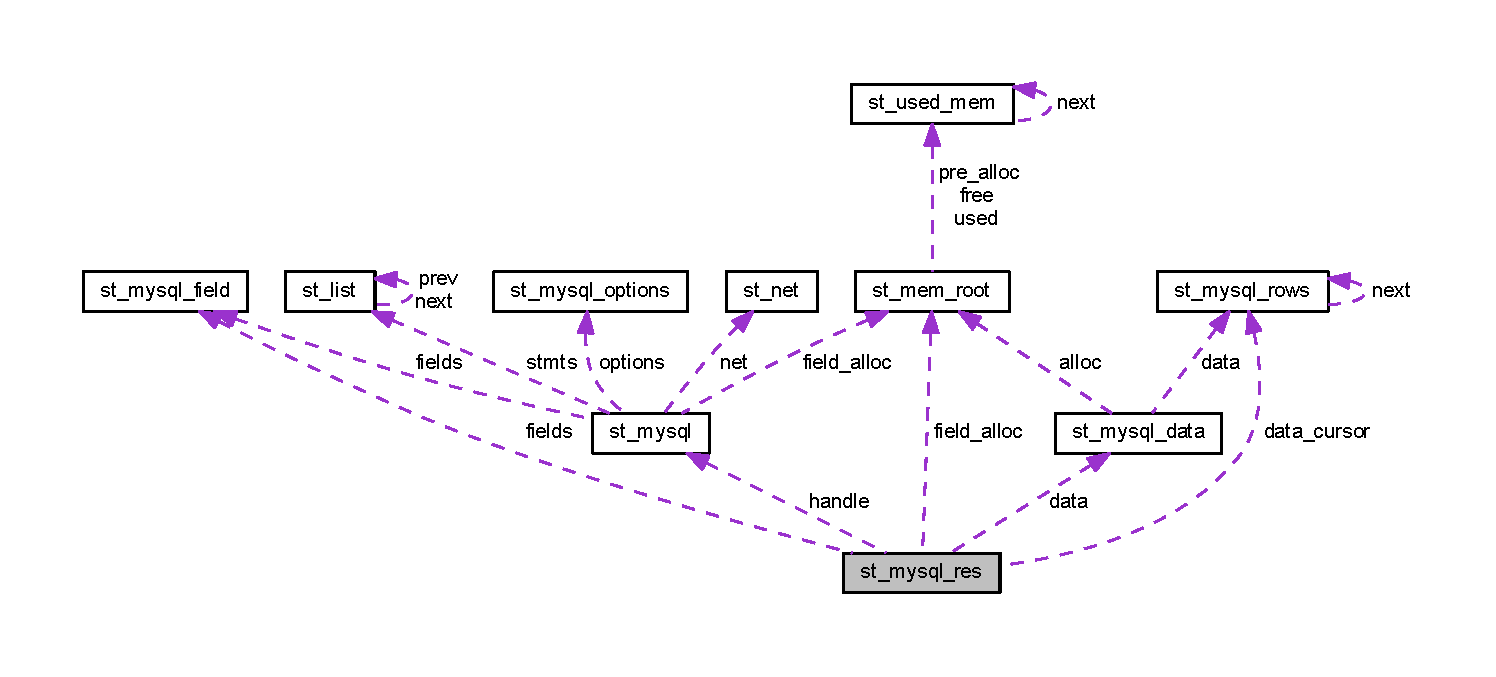
\includegraphics[width=350pt]{structst__mysql__res__coll__graph}
\end{center}
\end{figure}
\subsection*{Data Fields}
\begin{DoxyCompactItemize}
\item 
\hyperlink{mysql_8h_ae05bd5d3e5a75578e2f14cfeb43f07aa}{my\+\_\+ulonglong} \hyperlink{structst__mysql__res_aeebcaa8a317200a20bbde5d9f9f73169}{row\+\_\+count}
\item 
\hyperlink{mysql_8h_ad010774d7ae34dc28a2e044ed2cd4f71}{M\+Y\+S\+Q\+L\+\_\+\+F\+I\+E\+L\+D} $\ast$ \hyperlink{structst__mysql__res_a608224b643e0d8fc992de01230195dda}{fields}
\item 
\hyperlink{mysql_8h_a19837b8e2f5cec429a5b61d4d5c68ed6}{M\+Y\+S\+Q\+L\+\_\+\+D\+A\+T\+A} $\ast$ \hyperlink{structst__mysql__res_a213ea8e00645396f226362cdbd2880b7}{data}
\item 
\hyperlink{mysql_8h_a4d0140764825a51eae874c641df1afb5}{M\+Y\+S\+Q\+L\+\_\+\+R\+O\+W\+S} $\ast$ \hyperlink{structst__mysql__res_a874a24ee537561e5dc86e5e86a9afd9d}{data\+\_\+cursor}
\item 
unsigned long $\ast$ \hyperlink{structst__mysql__res_ac6b5b0d8456fe15d529ece8c107d7063}{lengths}
\item 
\hyperlink{mysql_8h_a42e5b5e53a1263817a59e42e219feca6}{M\+Y\+S\+Q\+L} $\ast$ \hyperlink{structst__mysql__res_ac67d314af96af560ea7880245ab5a710}{handle}
\item 
const struct st\+\_\+mysql\+\_\+methods $\ast$ \hyperlink{structst__mysql__res_a87d087d083eb50c81b30285a7b8458b1}{methods}
\item 
\hyperlink{mysql_8h_afae8ad264fb6a4bd740df59f19b9da71}{M\+Y\+S\+Q\+L\+\_\+\+R\+O\+W} \hyperlink{structst__mysql__res_a12b56773449e21072694f7749086d64a}{row}
\item 
\hyperlink{mysql_8h_afae8ad264fb6a4bd740df59f19b9da71}{M\+Y\+S\+Q\+L\+\_\+\+R\+O\+W} \hyperlink{structst__mysql__res_ae4ba04806b79944ca5c5cd46ff8b1ef2}{current\+\_\+row}
\item 
\hyperlink{my__alloc_8h_ac59e289b254a2c5ac634ffcedda3f823}{M\+E\+M\+\_\+\+R\+O\+O\+T} \hyperlink{structst__mysql__res_a76a8c7214ccdae2c8986b2f8bbc25dd2}{field\+\_\+alloc}
\item 
unsigned int \hyperlink{structst__mysql__res_a46ca3cf833b020e86e4d7f4ebe36f190}{field\+\_\+count}
\item 
unsigned int \hyperlink{structst__mysql__res_a35bcf75097f62db6990a09dcfd1d3401}{current\+\_\+field}
\item 
\hyperlink{mysql_8h_a74cd599039dcf29c6e6d342cf4efd0a8}{my\+\_\+bool} \hyperlink{structst__mysql__res_ab24839f1879e03ffa511e9bce92419e9}{eof}
\item 
\hyperlink{mysql_8h_a74cd599039dcf29c6e6d342cf4efd0a8}{my\+\_\+bool} \hyperlink{structst__mysql__res_a4fddbf81b6ead57fdfd384e74d918cfb}{unbuffered\+\_\+fetch\+\_\+cancelled}
\item 
void $\ast$ \hyperlink{structst__mysql__res_abf63f6350874811fdf3fb90c49e532dd}{extension}
\end{DoxyCompactItemize}


\subsection{Field Documentation}
\hypertarget{structst__mysql__res_a35bcf75097f62db6990a09dcfd1d3401}{}\index{st\+\_\+mysql\+\_\+res@{st\+\_\+mysql\+\_\+res}!current\+\_\+field@{current\+\_\+field}}
\index{current\+\_\+field@{current\+\_\+field}!st\+\_\+mysql\+\_\+res@{st\+\_\+mysql\+\_\+res}}
\subsubsection[{current\+\_\+field}]{\setlength{\rightskip}{0pt plus 5cm}unsigned int st\+\_\+mysql\+\_\+res\+::current\+\_\+field}\label{structst__mysql__res_a35bcf75097f62db6990a09dcfd1d3401}
\hypertarget{structst__mysql__res_ae4ba04806b79944ca5c5cd46ff8b1ef2}{}\index{st\+\_\+mysql\+\_\+res@{st\+\_\+mysql\+\_\+res}!current\+\_\+row@{current\+\_\+row}}
\index{current\+\_\+row@{current\+\_\+row}!st\+\_\+mysql\+\_\+res@{st\+\_\+mysql\+\_\+res}}
\subsubsection[{current\+\_\+row}]{\setlength{\rightskip}{0pt plus 5cm}{\bf M\+Y\+S\+Q\+L\+\_\+\+R\+O\+W} st\+\_\+mysql\+\_\+res\+::current\+\_\+row}\label{structst__mysql__res_ae4ba04806b79944ca5c5cd46ff8b1ef2}
\hypertarget{structst__mysql__res_a213ea8e00645396f226362cdbd2880b7}{}\index{st\+\_\+mysql\+\_\+res@{st\+\_\+mysql\+\_\+res}!data@{data}}
\index{data@{data}!st\+\_\+mysql\+\_\+res@{st\+\_\+mysql\+\_\+res}}
\subsubsection[{data}]{\setlength{\rightskip}{0pt plus 5cm}{\bf M\+Y\+S\+Q\+L\+\_\+\+D\+A\+T\+A}$\ast$ st\+\_\+mysql\+\_\+res\+::data}\label{structst__mysql__res_a213ea8e00645396f226362cdbd2880b7}
\hypertarget{structst__mysql__res_a874a24ee537561e5dc86e5e86a9afd9d}{}\index{st\+\_\+mysql\+\_\+res@{st\+\_\+mysql\+\_\+res}!data\+\_\+cursor@{data\+\_\+cursor}}
\index{data\+\_\+cursor@{data\+\_\+cursor}!st\+\_\+mysql\+\_\+res@{st\+\_\+mysql\+\_\+res}}
\subsubsection[{data\+\_\+cursor}]{\setlength{\rightskip}{0pt plus 5cm}{\bf M\+Y\+S\+Q\+L\+\_\+\+R\+O\+W\+S}$\ast$ st\+\_\+mysql\+\_\+res\+::data\+\_\+cursor}\label{structst__mysql__res_a874a24ee537561e5dc86e5e86a9afd9d}
\hypertarget{structst__mysql__res_ab24839f1879e03ffa511e9bce92419e9}{}\index{st\+\_\+mysql\+\_\+res@{st\+\_\+mysql\+\_\+res}!eof@{eof}}
\index{eof@{eof}!st\+\_\+mysql\+\_\+res@{st\+\_\+mysql\+\_\+res}}
\subsubsection[{eof}]{\setlength{\rightskip}{0pt plus 5cm}{\bf my\+\_\+bool} st\+\_\+mysql\+\_\+res\+::eof}\label{structst__mysql__res_ab24839f1879e03ffa511e9bce92419e9}
\hypertarget{structst__mysql__res_abf63f6350874811fdf3fb90c49e532dd}{}\index{st\+\_\+mysql\+\_\+res@{st\+\_\+mysql\+\_\+res}!extension@{extension}}
\index{extension@{extension}!st\+\_\+mysql\+\_\+res@{st\+\_\+mysql\+\_\+res}}
\subsubsection[{extension}]{\setlength{\rightskip}{0pt plus 5cm}void$\ast$ st\+\_\+mysql\+\_\+res\+::extension}\label{structst__mysql__res_abf63f6350874811fdf3fb90c49e532dd}
\hypertarget{structst__mysql__res_a76a8c7214ccdae2c8986b2f8bbc25dd2}{}\index{st\+\_\+mysql\+\_\+res@{st\+\_\+mysql\+\_\+res}!field\+\_\+alloc@{field\+\_\+alloc}}
\index{field\+\_\+alloc@{field\+\_\+alloc}!st\+\_\+mysql\+\_\+res@{st\+\_\+mysql\+\_\+res}}
\subsubsection[{field\+\_\+alloc}]{\setlength{\rightskip}{0pt plus 5cm}{\bf M\+E\+M\+\_\+\+R\+O\+O\+T} st\+\_\+mysql\+\_\+res\+::field\+\_\+alloc}\label{structst__mysql__res_a76a8c7214ccdae2c8986b2f8bbc25dd2}
\hypertarget{structst__mysql__res_a46ca3cf833b020e86e4d7f4ebe36f190}{}\index{st\+\_\+mysql\+\_\+res@{st\+\_\+mysql\+\_\+res}!field\+\_\+count@{field\+\_\+count}}
\index{field\+\_\+count@{field\+\_\+count}!st\+\_\+mysql\+\_\+res@{st\+\_\+mysql\+\_\+res}}
\subsubsection[{field\+\_\+count}]{\setlength{\rightskip}{0pt plus 5cm}unsigned int st\+\_\+mysql\+\_\+res\+::field\+\_\+count}\label{structst__mysql__res_a46ca3cf833b020e86e4d7f4ebe36f190}
\hypertarget{structst__mysql__res_a608224b643e0d8fc992de01230195dda}{}\index{st\+\_\+mysql\+\_\+res@{st\+\_\+mysql\+\_\+res}!fields@{fields}}
\index{fields@{fields}!st\+\_\+mysql\+\_\+res@{st\+\_\+mysql\+\_\+res}}
\subsubsection[{fields}]{\setlength{\rightskip}{0pt plus 5cm}{\bf M\+Y\+S\+Q\+L\+\_\+\+F\+I\+E\+L\+D}$\ast$ st\+\_\+mysql\+\_\+res\+::fields}\label{structst__mysql__res_a608224b643e0d8fc992de01230195dda}
\hypertarget{structst__mysql__res_ac67d314af96af560ea7880245ab5a710}{}\index{st\+\_\+mysql\+\_\+res@{st\+\_\+mysql\+\_\+res}!handle@{handle}}
\index{handle@{handle}!st\+\_\+mysql\+\_\+res@{st\+\_\+mysql\+\_\+res}}
\subsubsection[{handle}]{\setlength{\rightskip}{0pt plus 5cm}{\bf M\+Y\+S\+Q\+L}$\ast$ st\+\_\+mysql\+\_\+res\+::handle}\label{structst__mysql__res_ac67d314af96af560ea7880245ab5a710}
\hypertarget{structst__mysql__res_ac6b5b0d8456fe15d529ece8c107d7063}{}\index{st\+\_\+mysql\+\_\+res@{st\+\_\+mysql\+\_\+res}!lengths@{lengths}}
\index{lengths@{lengths}!st\+\_\+mysql\+\_\+res@{st\+\_\+mysql\+\_\+res}}
\subsubsection[{lengths}]{\setlength{\rightskip}{0pt plus 5cm}unsigned long$\ast$ st\+\_\+mysql\+\_\+res\+::lengths}\label{structst__mysql__res_ac6b5b0d8456fe15d529ece8c107d7063}
\hypertarget{structst__mysql__res_a87d087d083eb50c81b30285a7b8458b1}{}\index{st\+\_\+mysql\+\_\+res@{st\+\_\+mysql\+\_\+res}!methods@{methods}}
\index{methods@{methods}!st\+\_\+mysql\+\_\+res@{st\+\_\+mysql\+\_\+res}}
\subsubsection[{methods}]{\setlength{\rightskip}{0pt plus 5cm}const struct st\+\_\+mysql\+\_\+methods$\ast$ st\+\_\+mysql\+\_\+res\+::methods}\label{structst__mysql__res_a87d087d083eb50c81b30285a7b8458b1}
\hypertarget{structst__mysql__res_a12b56773449e21072694f7749086d64a}{}\index{st\+\_\+mysql\+\_\+res@{st\+\_\+mysql\+\_\+res}!row@{row}}
\index{row@{row}!st\+\_\+mysql\+\_\+res@{st\+\_\+mysql\+\_\+res}}
\subsubsection[{row}]{\setlength{\rightskip}{0pt plus 5cm}{\bf M\+Y\+S\+Q\+L\+\_\+\+R\+O\+W} st\+\_\+mysql\+\_\+res\+::row}\label{structst__mysql__res_a12b56773449e21072694f7749086d64a}
\hypertarget{structst__mysql__res_aeebcaa8a317200a20bbde5d9f9f73169}{}\index{st\+\_\+mysql\+\_\+res@{st\+\_\+mysql\+\_\+res}!row\+\_\+count@{row\+\_\+count}}
\index{row\+\_\+count@{row\+\_\+count}!st\+\_\+mysql\+\_\+res@{st\+\_\+mysql\+\_\+res}}
\subsubsection[{row\+\_\+count}]{\setlength{\rightskip}{0pt plus 5cm}{\bf my\+\_\+ulonglong} st\+\_\+mysql\+\_\+res\+::row\+\_\+count}\label{structst__mysql__res_aeebcaa8a317200a20bbde5d9f9f73169}
\hypertarget{structst__mysql__res_a4fddbf81b6ead57fdfd384e74d918cfb}{}\index{st\+\_\+mysql\+\_\+res@{st\+\_\+mysql\+\_\+res}!unbuffered\+\_\+fetch\+\_\+cancelled@{unbuffered\+\_\+fetch\+\_\+cancelled}}
\index{unbuffered\+\_\+fetch\+\_\+cancelled@{unbuffered\+\_\+fetch\+\_\+cancelled}!st\+\_\+mysql\+\_\+res@{st\+\_\+mysql\+\_\+res}}
\subsubsection[{unbuffered\+\_\+fetch\+\_\+cancelled}]{\setlength{\rightskip}{0pt plus 5cm}{\bf my\+\_\+bool} st\+\_\+mysql\+\_\+res\+::unbuffered\+\_\+fetch\+\_\+cancelled}\label{structst__mysql__res_a4fddbf81b6ead57fdfd384e74d918cfb}


The documentation for this struct was generated from the following file\+:\begin{DoxyCompactItemize}
\item 
\hyperlink{mysql_8h}{mysql.\+h}\end{DoxyCompactItemize}

\hypertarget{structst__mysql__rows}{}\section{st\+\_\+mysql\+\_\+rows Struct Reference}
\label{structst__mysql__rows}\index{st\+\_\+mysql\+\_\+rows@{st\+\_\+mysql\+\_\+rows}}


{\ttfamily \#include $<$mysql.\+h$>$}



Collaboration diagram for st\+\_\+mysql\+\_\+rows\+:\nopagebreak
\begin{figure}[H]
\begin{center}
\leavevmode
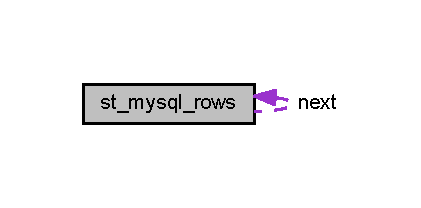
\includegraphics[width=202pt]{structst__mysql__rows__coll__graph}
\end{center}
\end{figure}
\subsection*{Data Fields}
\begin{DoxyCompactItemize}
\item 
struct \hyperlink{structst__mysql__rows}{st\+\_\+mysql\+\_\+rows} $\ast$ \hyperlink{structst__mysql__rows_a83f438b68306724f8fd2f35758bbb2f7}{next}
\item 
\hyperlink{mysql_8h_afae8ad264fb6a4bd740df59f19b9da71}{M\+Y\+S\+Q\+L\+\_\+\+R\+O\+W} \hyperlink{structst__mysql__rows_a9e11c8188cb52a253df7ac713751b5e2}{data}
\item 
unsigned long \hyperlink{structst__mysql__rows_ae0da25ba59a9ef9c4e148664b3db13af}{length}
\end{DoxyCompactItemize}


\subsection{Field Documentation}
\hypertarget{structst__mysql__rows_a9e11c8188cb52a253df7ac713751b5e2}{}\index{st\+\_\+mysql\+\_\+rows@{st\+\_\+mysql\+\_\+rows}!data@{data}}
\index{data@{data}!st\+\_\+mysql\+\_\+rows@{st\+\_\+mysql\+\_\+rows}}
\subsubsection[{data}]{\setlength{\rightskip}{0pt plus 5cm}{\bf M\+Y\+S\+Q\+L\+\_\+\+R\+O\+W} st\+\_\+mysql\+\_\+rows\+::data}\label{structst__mysql__rows_a9e11c8188cb52a253df7ac713751b5e2}
\hypertarget{structst__mysql__rows_ae0da25ba59a9ef9c4e148664b3db13af}{}\index{st\+\_\+mysql\+\_\+rows@{st\+\_\+mysql\+\_\+rows}!length@{length}}
\index{length@{length}!st\+\_\+mysql\+\_\+rows@{st\+\_\+mysql\+\_\+rows}}
\subsubsection[{length}]{\setlength{\rightskip}{0pt plus 5cm}unsigned long st\+\_\+mysql\+\_\+rows\+::length}\label{structst__mysql__rows_ae0da25ba59a9ef9c4e148664b3db13af}
\hypertarget{structst__mysql__rows_a83f438b68306724f8fd2f35758bbb2f7}{}\index{st\+\_\+mysql\+\_\+rows@{st\+\_\+mysql\+\_\+rows}!next@{next}}
\index{next@{next}!st\+\_\+mysql\+\_\+rows@{st\+\_\+mysql\+\_\+rows}}
\subsubsection[{next}]{\setlength{\rightskip}{0pt plus 5cm}struct {\bf st\+\_\+mysql\+\_\+rows}$\ast$ st\+\_\+mysql\+\_\+rows\+::next}\label{structst__mysql__rows_a83f438b68306724f8fd2f35758bbb2f7}


The documentation for this struct was generated from the following file\+:\begin{DoxyCompactItemize}
\item 
\hyperlink{mysql_8h}{mysql.\+h}\end{DoxyCompactItemize}

\hypertarget{structst__mysql__stmt}{}\section{st\+\_\+mysql\+\_\+stmt Struct Reference}
\label{structst__mysql__stmt}\index{st\+\_\+mysql\+\_\+stmt@{st\+\_\+mysql\+\_\+stmt}}


{\ttfamily \#include $<$mysql.\+h$>$}



Collaboration diagram for st\+\_\+mysql\+\_\+stmt\+:\nopagebreak
\begin{figure}[H]
\begin{center}
\leavevmode
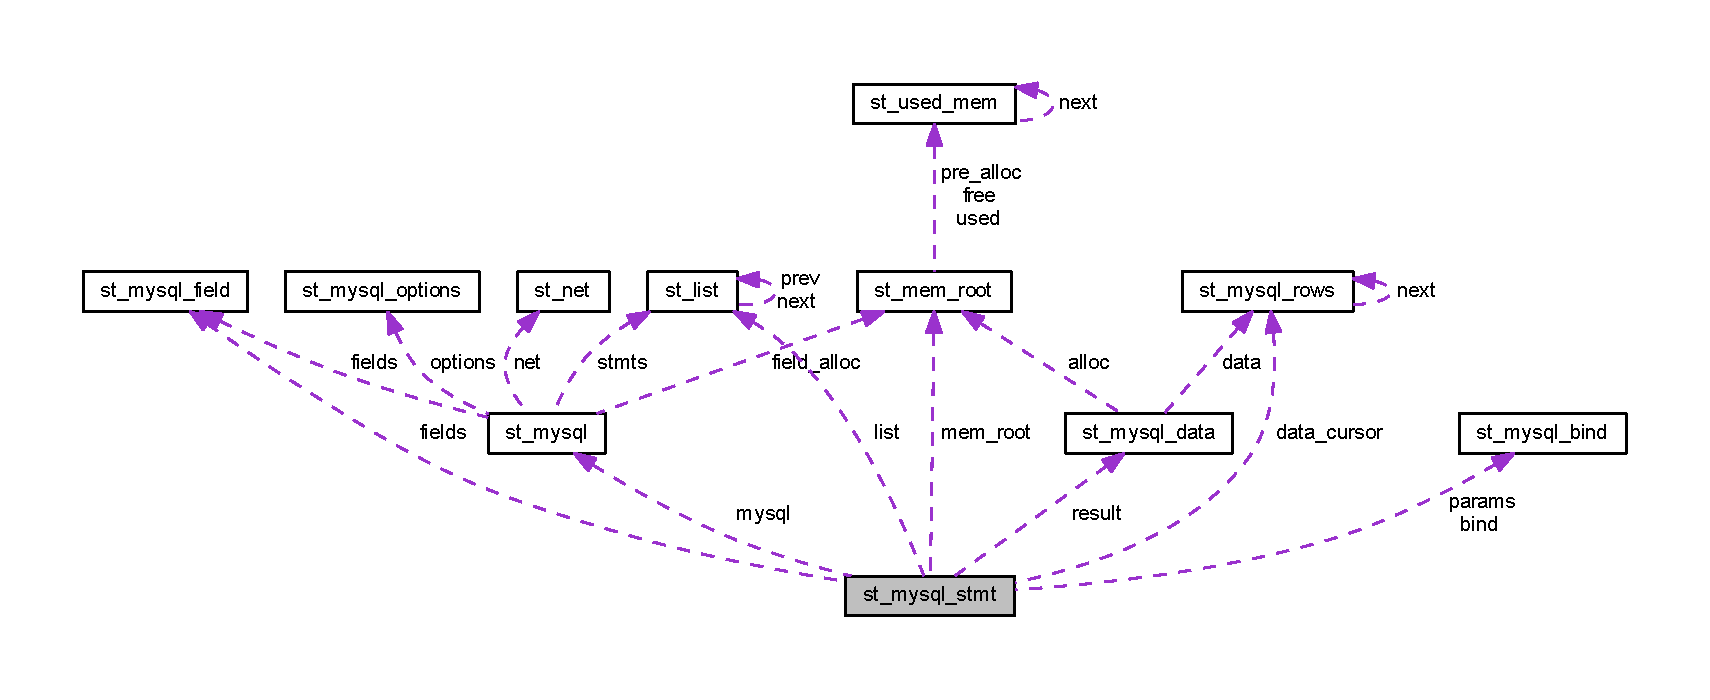
\includegraphics[width=350pt]{structst__mysql__stmt__coll__graph}
\end{center}
\end{figure}
\subsection*{Data Fields}
\begin{DoxyCompactItemize}
\item 
\hyperlink{my__alloc_8h_ac59e289b254a2c5ac634ffcedda3f823}{M\+E\+M\+\_\+\+R\+O\+O\+T} \hyperlink{structst__mysql__stmt_a292686a1de9fdbddc3963bcf20249cb0}{mem\+\_\+root}
\item 
\hyperlink{my__list_8h_ab2a1c5fd766481fe9ec169b9fdca184e}{L\+I\+S\+T} \hyperlink{structst__mysql__stmt_aac96a0c9f7a07434da3d798f3b2ece87}{list}
\item 
\hyperlink{mysql_8h_a42e5b5e53a1263817a59e42e219feca6}{M\+Y\+S\+Q\+L} $\ast$ \hyperlink{structst__mysql__stmt_a224349871acc052c72cfa86f5901c809}{mysql}
\item 
\hyperlink{mysql_8h_a4cec8aef3d6aab1d7d9d8e4f2a90457d}{M\+Y\+S\+Q\+L\+\_\+\+B\+I\+N\+D} $\ast$ \hyperlink{structst__mysql__stmt_a0276e0f80817dccc03611786fd646ec7}{params}
\item 
\hyperlink{mysql_8h_a4cec8aef3d6aab1d7d9d8e4f2a90457d}{M\+Y\+S\+Q\+L\+\_\+\+B\+I\+N\+D} $\ast$ \hyperlink{structst__mysql__stmt_a5651622ae4c2c31616aa648b70cc12b2}{bind}
\item 
\hyperlink{mysql_8h_ad010774d7ae34dc28a2e044ed2cd4f71}{M\+Y\+S\+Q\+L\+\_\+\+F\+I\+E\+L\+D} $\ast$ \hyperlink{structst__mysql__stmt_a1d7627383d3c0ab2989968d88c2bb83d}{fields}
\item 
\hyperlink{mysql_8h_a19837b8e2f5cec429a5b61d4d5c68ed6}{M\+Y\+S\+Q\+L\+\_\+\+D\+A\+T\+A} \hyperlink{structst__mysql__stmt_a198cbcc8f7faf73522a281dec2e1e434}{result}
\item 
\hyperlink{mysql_8h_a4d0140764825a51eae874c641df1afb5}{M\+Y\+S\+Q\+L\+\_\+\+R\+O\+W\+S} $\ast$ \hyperlink{structst__mysql__stmt_ad1663e8fd4bab5be184b6cd38d3296f8}{data\+\_\+cursor}
\item 
int($\ast$ \hyperlink{structst__mysql__stmt_a908e910a9ff3cf311f2a34408179cffe}{read\+\_\+row\+\_\+func} )(struct \hyperlink{structst__mysql__stmt}{st\+\_\+mysql\+\_\+stmt} $\ast$stmt, unsigned char $\ast$$\ast$row)
\item 
\hyperlink{mysql_8h_ae05bd5d3e5a75578e2f14cfeb43f07aa}{my\+\_\+ulonglong} \hyperlink{structst__mysql__stmt_af168ff6c13b33aca298c39d5b128f428}{affected\+\_\+rows}
\item 
\hyperlink{mysql_8h_ae05bd5d3e5a75578e2f14cfeb43f07aa}{my\+\_\+ulonglong} \hyperlink{structst__mysql__stmt_ae1412a9a6bacafb7daf66f5fc826b54f}{insert\+\_\+id}
\item 
unsigned long \hyperlink{structst__mysql__stmt_ad800f40b351919f8d6e9c9a4d757ab72}{stmt\+\_\+id}
\item 
unsigned long \hyperlink{structst__mysql__stmt_a5db08a5ec03692af1fd1b2d588c10999}{flags}
\item 
unsigned long \hyperlink{structst__mysql__stmt_ae2e891ae11a6f5d016166f93d1553c24}{prefetch\+\_\+rows}
\item 
unsigned int \hyperlink{structst__mysql__stmt_af2b6c14f77e053b0cb952f4bc838a94a}{server\+\_\+status}
\item 
unsigned int \hyperlink{structst__mysql__stmt_a58c9c8e23ee17b61de9804585fa3c9cd}{last\+\_\+errno}
\item 
unsigned int \hyperlink{structst__mysql__stmt_a082d2c41726787a2c9daea75e9afb2cd}{param\+\_\+count}
\item 
unsigned int \hyperlink{structst__mysql__stmt_aee56a3ffa9c1019c207ee1eaade2306b}{field\+\_\+count}
\item 
enum \hyperlink{mysql_8h_a3491e6b32b8b2a22404cc3c009343b63}{enum\+\_\+mysql\+\_\+stmt\+\_\+state} \hyperlink{structst__mysql__stmt_a30dfb09d512d7b9397f8bea13bfc319b}{state}
\item 
char \hyperlink{structst__mysql__stmt_a5aa67e24109cb953e09d788756802c9a}{last\+\_\+error} \mbox{[}\hyperlink{mysql__com_8h_a3f5f3eab30894e1dfa8d5bd977a889be}{M\+Y\+S\+Q\+L\+\_\+\+E\+R\+R\+M\+S\+G\+\_\+\+S\+I\+Z\+E}\mbox{]}
\item 
char \hyperlink{structst__mysql__stmt_a4bc2da06a308a95a0e5af923239493b5}{sqlstate} \mbox{[}\hyperlink{mysql__com_8h_a8e152edf1a0bae8aec7f5d59cebfbea9}{S\+Q\+L\+S\+T\+A\+T\+E\+\_\+\+L\+E\+N\+G\+T\+H}+1\mbox{]}
\item 
\hyperlink{mysql_8h_a74cd599039dcf29c6e6d342cf4efd0a8}{my\+\_\+bool} \hyperlink{structst__mysql__stmt_a18b9cca9708b5d7ac8dba93f68e8da9c}{send\+\_\+types\+\_\+to\+\_\+server}
\item 
\hyperlink{mysql_8h_a74cd599039dcf29c6e6d342cf4efd0a8}{my\+\_\+bool} \hyperlink{structst__mysql__stmt_a591d90535b12361e5eb35142cead78cd}{bind\+\_\+param\+\_\+done}
\item 
unsigned char \hyperlink{structst__mysql__stmt_a0371a2667da810cfb863de6d15f5c24e}{bind\+\_\+result\+\_\+done}
\item 
\hyperlink{mysql_8h_a74cd599039dcf29c6e6d342cf4efd0a8}{my\+\_\+bool} \hyperlink{structst__mysql__stmt_aa0fee515cb67c6671540a12042362619}{unbuffered\+\_\+fetch\+\_\+cancelled}
\item 
\hyperlink{mysql_8h_a74cd599039dcf29c6e6d342cf4efd0a8}{my\+\_\+bool} \hyperlink{structst__mysql__stmt_ab2e8f874563ad8a2d658117548983cf8}{update\+\_\+max\+\_\+length}
\item 
struct st\+\_\+mysql\+\_\+stmt\+\_\+extension $\ast$ \hyperlink{structst__mysql__stmt_a7dc80b5b01da1a6ef0f18f2c41b3c1a0}{extension}
\end{DoxyCompactItemize}


\subsection{Field Documentation}
\hypertarget{structst__mysql__stmt_af168ff6c13b33aca298c39d5b128f428}{}\index{st\+\_\+mysql\+\_\+stmt@{st\+\_\+mysql\+\_\+stmt}!affected\+\_\+rows@{affected\+\_\+rows}}
\index{affected\+\_\+rows@{affected\+\_\+rows}!st\+\_\+mysql\+\_\+stmt@{st\+\_\+mysql\+\_\+stmt}}
\subsubsection[{affected\+\_\+rows}]{\setlength{\rightskip}{0pt plus 5cm}{\bf my\+\_\+ulonglong} st\+\_\+mysql\+\_\+stmt\+::affected\+\_\+rows}\label{structst__mysql__stmt_af168ff6c13b33aca298c39d5b128f428}
\hypertarget{structst__mysql__stmt_a5651622ae4c2c31616aa648b70cc12b2}{}\index{st\+\_\+mysql\+\_\+stmt@{st\+\_\+mysql\+\_\+stmt}!bind@{bind}}
\index{bind@{bind}!st\+\_\+mysql\+\_\+stmt@{st\+\_\+mysql\+\_\+stmt}}
\subsubsection[{bind}]{\setlength{\rightskip}{0pt plus 5cm}{\bf M\+Y\+S\+Q\+L\+\_\+\+B\+I\+N\+D}$\ast$ st\+\_\+mysql\+\_\+stmt\+::bind}\label{structst__mysql__stmt_a5651622ae4c2c31616aa648b70cc12b2}
\hypertarget{structst__mysql__stmt_a591d90535b12361e5eb35142cead78cd}{}\index{st\+\_\+mysql\+\_\+stmt@{st\+\_\+mysql\+\_\+stmt}!bind\+\_\+param\+\_\+done@{bind\+\_\+param\+\_\+done}}
\index{bind\+\_\+param\+\_\+done@{bind\+\_\+param\+\_\+done}!st\+\_\+mysql\+\_\+stmt@{st\+\_\+mysql\+\_\+stmt}}
\subsubsection[{bind\+\_\+param\+\_\+done}]{\setlength{\rightskip}{0pt plus 5cm}{\bf my\+\_\+bool} st\+\_\+mysql\+\_\+stmt\+::bind\+\_\+param\+\_\+done}\label{structst__mysql__stmt_a591d90535b12361e5eb35142cead78cd}
\hypertarget{structst__mysql__stmt_a0371a2667da810cfb863de6d15f5c24e}{}\index{st\+\_\+mysql\+\_\+stmt@{st\+\_\+mysql\+\_\+stmt}!bind\+\_\+result\+\_\+done@{bind\+\_\+result\+\_\+done}}
\index{bind\+\_\+result\+\_\+done@{bind\+\_\+result\+\_\+done}!st\+\_\+mysql\+\_\+stmt@{st\+\_\+mysql\+\_\+stmt}}
\subsubsection[{bind\+\_\+result\+\_\+done}]{\setlength{\rightskip}{0pt plus 5cm}unsigned char st\+\_\+mysql\+\_\+stmt\+::bind\+\_\+result\+\_\+done}\label{structst__mysql__stmt_a0371a2667da810cfb863de6d15f5c24e}
\hypertarget{structst__mysql__stmt_ad1663e8fd4bab5be184b6cd38d3296f8}{}\index{st\+\_\+mysql\+\_\+stmt@{st\+\_\+mysql\+\_\+stmt}!data\+\_\+cursor@{data\+\_\+cursor}}
\index{data\+\_\+cursor@{data\+\_\+cursor}!st\+\_\+mysql\+\_\+stmt@{st\+\_\+mysql\+\_\+stmt}}
\subsubsection[{data\+\_\+cursor}]{\setlength{\rightskip}{0pt plus 5cm}{\bf M\+Y\+S\+Q\+L\+\_\+\+R\+O\+W\+S}$\ast$ st\+\_\+mysql\+\_\+stmt\+::data\+\_\+cursor}\label{structst__mysql__stmt_ad1663e8fd4bab5be184b6cd38d3296f8}
\hypertarget{structst__mysql__stmt_a7dc80b5b01da1a6ef0f18f2c41b3c1a0}{}\index{st\+\_\+mysql\+\_\+stmt@{st\+\_\+mysql\+\_\+stmt}!extension@{extension}}
\index{extension@{extension}!st\+\_\+mysql\+\_\+stmt@{st\+\_\+mysql\+\_\+stmt}}
\subsubsection[{extension}]{\setlength{\rightskip}{0pt plus 5cm}struct st\+\_\+mysql\+\_\+stmt\+\_\+extension$\ast$ st\+\_\+mysql\+\_\+stmt\+::extension}\label{structst__mysql__stmt_a7dc80b5b01da1a6ef0f18f2c41b3c1a0}
\hypertarget{structst__mysql__stmt_aee56a3ffa9c1019c207ee1eaade2306b}{}\index{st\+\_\+mysql\+\_\+stmt@{st\+\_\+mysql\+\_\+stmt}!field\+\_\+count@{field\+\_\+count}}
\index{field\+\_\+count@{field\+\_\+count}!st\+\_\+mysql\+\_\+stmt@{st\+\_\+mysql\+\_\+stmt}}
\subsubsection[{field\+\_\+count}]{\setlength{\rightskip}{0pt plus 5cm}unsigned int st\+\_\+mysql\+\_\+stmt\+::field\+\_\+count}\label{structst__mysql__stmt_aee56a3ffa9c1019c207ee1eaade2306b}
\hypertarget{structst__mysql__stmt_a1d7627383d3c0ab2989968d88c2bb83d}{}\index{st\+\_\+mysql\+\_\+stmt@{st\+\_\+mysql\+\_\+stmt}!fields@{fields}}
\index{fields@{fields}!st\+\_\+mysql\+\_\+stmt@{st\+\_\+mysql\+\_\+stmt}}
\subsubsection[{fields}]{\setlength{\rightskip}{0pt plus 5cm}{\bf M\+Y\+S\+Q\+L\+\_\+\+F\+I\+E\+L\+D}$\ast$ st\+\_\+mysql\+\_\+stmt\+::fields}\label{structst__mysql__stmt_a1d7627383d3c0ab2989968d88c2bb83d}
\hypertarget{structst__mysql__stmt_a5db08a5ec03692af1fd1b2d588c10999}{}\index{st\+\_\+mysql\+\_\+stmt@{st\+\_\+mysql\+\_\+stmt}!flags@{flags}}
\index{flags@{flags}!st\+\_\+mysql\+\_\+stmt@{st\+\_\+mysql\+\_\+stmt}}
\subsubsection[{flags}]{\setlength{\rightskip}{0pt plus 5cm}unsigned long st\+\_\+mysql\+\_\+stmt\+::flags}\label{structst__mysql__stmt_a5db08a5ec03692af1fd1b2d588c10999}
\hypertarget{structst__mysql__stmt_ae1412a9a6bacafb7daf66f5fc826b54f}{}\index{st\+\_\+mysql\+\_\+stmt@{st\+\_\+mysql\+\_\+stmt}!insert\+\_\+id@{insert\+\_\+id}}
\index{insert\+\_\+id@{insert\+\_\+id}!st\+\_\+mysql\+\_\+stmt@{st\+\_\+mysql\+\_\+stmt}}
\subsubsection[{insert\+\_\+id}]{\setlength{\rightskip}{0pt plus 5cm}{\bf my\+\_\+ulonglong} st\+\_\+mysql\+\_\+stmt\+::insert\+\_\+id}\label{structst__mysql__stmt_ae1412a9a6bacafb7daf66f5fc826b54f}
\hypertarget{structst__mysql__stmt_a58c9c8e23ee17b61de9804585fa3c9cd}{}\index{st\+\_\+mysql\+\_\+stmt@{st\+\_\+mysql\+\_\+stmt}!last\+\_\+errno@{last\+\_\+errno}}
\index{last\+\_\+errno@{last\+\_\+errno}!st\+\_\+mysql\+\_\+stmt@{st\+\_\+mysql\+\_\+stmt}}
\subsubsection[{last\+\_\+errno}]{\setlength{\rightskip}{0pt plus 5cm}unsigned int st\+\_\+mysql\+\_\+stmt\+::last\+\_\+errno}\label{structst__mysql__stmt_a58c9c8e23ee17b61de9804585fa3c9cd}
\hypertarget{structst__mysql__stmt_a5aa67e24109cb953e09d788756802c9a}{}\index{st\+\_\+mysql\+\_\+stmt@{st\+\_\+mysql\+\_\+stmt}!last\+\_\+error@{last\+\_\+error}}
\index{last\+\_\+error@{last\+\_\+error}!st\+\_\+mysql\+\_\+stmt@{st\+\_\+mysql\+\_\+stmt}}
\subsubsection[{last\+\_\+error}]{\setlength{\rightskip}{0pt plus 5cm}char st\+\_\+mysql\+\_\+stmt\+::last\+\_\+error\mbox{[}{\bf M\+Y\+S\+Q\+L\+\_\+\+E\+R\+R\+M\+S\+G\+\_\+\+S\+I\+Z\+E}\mbox{]}}\label{structst__mysql__stmt_a5aa67e24109cb953e09d788756802c9a}
\hypertarget{structst__mysql__stmt_aac96a0c9f7a07434da3d798f3b2ece87}{}\index{st\+\_\+mysql\+\_\+stmt@{st\+\_\+mysql\+\_\+stmt}!list@{list}}
\index{list@{list}!st\+\_\+mysql\+\_\+stmt@{st\+\_\+mysql\+\_\+stmt}}
\subsubsection[{list}]{\setlength{\rightskip}{0pt plus 5cm}{\bf L\+I\+S\+T} st\+\_\+mysql\+\_\+stmt\+::list}\label{structst__mysql__stmt_aac96a0c9f7a07434da3d798f3b2ece87}
\hypertarget{structst__mysql__stmt_a292686a1de9fdbddc3963bcf20249cb0}{}\index{st\+\_\+mysql\+\_\+stmt@{st\+\_\+mysql\+\_\+stmt}!mem\+\_\+root@{mem\+\_\+root}}
\index{mem\+\_\+root@{mem\+\_\+root}!st\+\_\+mysql\+\_\+stmt@{st\+\_\+mysql\+\_\+stmt}}
\subsubsection[{mem\+\_\+root}]{\setlength{\rightskip}{0pt plus 5cm}{\bf M\+E\+M\+\_\+\+R\+O\+O\+T} st\+\_\+mysql\+\_\+stmt\+::mem\+\_\+root}\label{structst__mysql__stmt_a292686a1de9fdbddc3963bcf20249cb0}
\hypertarget{structst__mysql__stmt_a224349871acc052c72cfa86f5901c809}{}\index{st\+\_\+mysql\+\_\+stmt@{st\+\_\+mysql\+\_\+stmt}!mysql@{mysql}}
\index{mysql@{mysql}!st\+\_\+mysql\+\_\+stmt@{st\+\_\+mysql\+\_\+stmt}}
\subsubsection[{mysql}]{\setlength{\rightskip}{0pt plus 5cm}{\bf M\+Y\+S\+Q\+L}$\ast$ st\+\_\+mysql\+\_\+stmt\+::mysql}\label{structst__mysql__stmt_a224349871acc052c72cfa86f5901c809}
\hypertarget{structst__mysql__stmt_a082d2c41726787a2c9daea75e9afb2cd}{}\index{st\+\_\+mysql\+\_\+stmt@{st\+\_\+mysql\+\_\+stmt}!param\+\_\+count@{param\+\_\+count}}
\index{param\+\_\+count@{param\+\_\+count}!st\+\_\+mysql\+\_\+stmt@{st\+\_\+mysql\+\_\+stmt}}
\subsubsection[{param\+\_\+count}]{\setlength{\rightskip}{0pt plus 5cm}unsigned int st\+\_\+mysql\+\_\+stmt\+::param\+\_\+count}\label{structst__mysql__stmt_a082d2c41726787a2c9daea75e9afb2cd}
\hypertarget{structst__mysql__stmt_a0276e0f80817dccc03611786fd646ec7}{}\index{st\+\_\+mysql\+\_\+stmt@{st\+\_\+mysql\+\_\+stmt}!params@{params}}
\index{params@{params}!st\+\_\+mysql\+\_\+stmt@{st\+\_\+mysql\+\_\+stmt}}
\subsubsection[{params}]{\setlength{\rightskip}{0pt plus 5cm}{\bf M\+Y\+S\+Q\+L\+\_\+\+B\+I\+N\+D}$\ast$ st\+\_\+mysql\+\_\+stmt\+::params}\label{structst__mysql__stmt_a0276e0f80817dccc03611786fd646ec7}
\hypertarget{structst__mysql__stmt_ae2e891ae11a6f5d016166f93d1553c24}{}\index{st\+\_\+mysql\+\_\+stmt@{st\+\_\+mysql\+\_\+stmt}!prefetch\+\_\+rows@{prefetch\+\_\+rows}}
\index{prefetch\+\_\+rows@{prefetch\+\_\+rows}!st\+\_\+mysql\+\_\+stmt@{st\+\_\+mysql\+\_\+stmt}}
\subsubsection[{prefetch\+\_\+rows}]{\setlength{\rightskip}{0pt plus 5cm}unsigned long st\+\_\+mysql\+\_\+stmt\+::prefetch\+\_\+rows}\label{structst__mysql__stmt_ae2e891ae11a6f5d016166f93d1553c24}
\hypertarget{structst__mysql__stmt_a908e910a9ff3cf311f2a34408179cffe}{}\index{st\+\_\+mysql\+\_\+stmt@{st\+\_\+mysql\+\_\+stmt}!read\+\_\+row\+\_\+func@{read\+\_\+row\+\_\+func}}
\index{read\+\_\+row\+\_\+func@{read\+\_\+row\+\_\+func}!st\+\_\+mysql\+\_\+stmt@{st\+\_\+mysql\+\_\+stmt}}
\subsubsection[{read\+\_\+row\+\_\+func}]{\setlength{\rightskip}{0pt plus 5cm}int($\ast$ st\+\_\+mysql\+\_\+stmt\+::read\+\_\+row\+\_\+func) (struct {\bf st\+\_\+mysql\+\_\+stmt} $\ast$stmt, unsigned char $\ast$$\ast$row)}\label{structst__mysql__stmt_a908e910a9ff3cf311f2a34408179cffe}
\hypertarget{structst__mysql__stmt_a198cbcc8f7faf73522a281dec2e1e434}{}\index{st\+\_\+mysql\+\_\+stmt@{st\+\_\+mysql\+\_\+stmt}!result@{result}}
\index{result@{result}!st\+\_\+mysql\+\_\+stmt@{st\+\_\+mysql\+\_\+stmt}}
\subsubsection[{result}]{\setlength{\rightskip}{0pt plus 5cm}{\bf M\+Y\+S\+Q\+L\+\_\+\+D\+A\+T\+A} st\+\_\+mysql\+\_\+stmt\+::result}\label{structst__mysql__stmt_a198cbcc8f7faf73522a281dec2e1e434}
\hypertarget{structst__mysql__stmt_a18b9cca9708b5d7ac8dba93f68e8da9c}{}\index{st\+\_\+mysql\+\_\+stmt@{st\+\_\+mysql\+\_\+stmt}!send\+\_\+types\+\_\+to\+\_\+server@{send\+\_\+types\+\_\+to\+\_\+server}}
\index{send\+\_\+types\+\_\+to\+\_\+server@{send\+\_\+types\+\_\+to\+\_\+server}!st\+\_\+mysql\+\_\+stmt@{st\+\_\+mysql\+\_\+stmt}}
\subsubsection[{send\+\_\+types\+\_\+to\+\_\+server}]{\setlength{\rightskip}{0pt plus 5cm}{\bf my\+\_\+bool} st\+\_\+mysql\+\_\+stmt\+::send\+\_\+types\+\_\+to\+\_\+server}\label{structst__mysql__stmt_a18b9cca9708b5d7ac8dba93f68e8da9c}
\hypertarget{structst__mysql__stmt_af2b6c14f77e053b0cb952f4bc838a94a}{}\index{st\+\_\+mysql\+\_\+stmt@{st\+\_\+mysql\+\_\+stmt}!server\+\_\+status@{server\+\_\+status}}
\index{server\+\_\+status@{server\+\_\+status}!st\+\_\+mysql\+\_\+stmt@{st\+\_\+mysql\+\_\+stmt}}
\subsubsection[{server\+\_\+status}]{\setlength{\rightskip}{0pt plus 5cm}unsigned int st\+\_\+mysql\+\_\+stmt\+::server\+\_\+status}\label{structst__mysql__stmt_af2b6c14f77e053b0cb952f4bc838a94a}
\hypertarget{structst__mysql__stmt_a4bc2da06a308a95a0e5af923239493b5}{}\index{st\+\_\+mysql\+\_\+stmt@{st\+\_\+mysql\+\_\+stmt}!sqlstate@{sqlstate}}
\index{sqlstate@{sqlstate}!st\+\_\+mysql\+\_\+stmt@{st\+\_\+mysql\+\_\+stmt}}
\subsubsection[{sqlstate}]{\setlength{\rightskip}{0pt plus 5cm}char st\+\_\+mysql\+\_\+stmt\+::sqlstate\mbox{[}{\bf S\+Q\+L\+S\+T\+A\+T\+E\+\_\+\+L\+E\+N\+G\+T\+H}+1\mbox{]}}\label{structst__mysql__stmt_a4bc2da06a308a95a0e5af923239493b5}
\hypertarget{structst__mysql__stmt_a30dfb09d512d7b9397f8bea13bfc319b}{}\index{st\+\_\+mysql\+\_\+stmt@{st\+\_\+mysql\+\_\+stmt}!state@{state}}
\index{state@{state}!st\+\_\+mysql\+\_\+stmt@{st\+\_\+mysql\+\_\+stmt}}
\subsubsection[{state}]{\setlength{\rightskip}{0pt plus 5cm}enum {\bf enum\+\_\+mysql\+\_\+stmt\+\_\+state} st\+\_\+mysql\+\_\+stmt\+::state}\label{structst__mysql__stmt_a30dfb09d512d7b9397f8bea13bfc319b}
\hypertarget{structst__mysql__stmt_ad800f40b351919f8d6e9c9a4d757ab72}{}\index{st\+\_\+mysql\+\_\+stmt@{st\+\_\+mysql\+\_\+stmt}!stmt\+\_\+id@{stmt\+\_\+id}}
\index{stmt\+\_\+id@{stmt\+\_\+id}!st\+\_\+mysql\+\_\+stmt@{st\+\_\+mysql\+\_\+stmt}}
\subsubsection[{stmt\+\_\+id}]{\setlength{\rightskip}{0pt plus 5cm}unsigned long st\+\_\+mysql\+\_\+stmt\+::stmt\+\_\+id}\label{structst__mysql__stmt_ad800f40b351919f8d6e9c9a4d757ab72}
\hypertarget{structst__mysql__stmt_aa0fee515cb67c6671540a12042362619}{}\index{st\+\_\+mysql\+\_\+stmt@{st\+\_\+mysql\+\_\+stmt}!unbuffered\+\_\+fetch\+\_\+cancelled@{unbuffered\+\_\+fetch\+\_\+cancelled}}
\index{unbuffered\+\_\+fetch\+\_\+cancelled@{unbuffered\+\_\+fetch\+\_\+cancelled}!st\+\_\+mysql\+\_\+stmt@{st\+\_\+mysql\+\_\+stmt}}
\subsubsection[{unbuffered\+\_\+fetch\+\_\+cancelled}]{\setlength{\rightskip}{0pt plus 5cm}{\bf my\+\_\+bool} st\+\_\+mysql\+\_\+stmt\+::unbuffered\+\_\+fetch\+\_\+cancelled}\label{structst__mysql__stmt_aa0fee515cb67c6671540a12042362619}
\hypertarget{structst__mysql__stmt_ab2e8f874563ad8a2d658117548983cf8}{}\index{st\+\_\+mysql\+\_\+stmt@{st\+\_\+mysql\+\_\+stmt}!update\+\_\+max\+\_\+length@{update\+\_\+max\+\_\+length}}
\index{update\+\_\+max\+\_\+length@{update\+\_\+max\+\_\+length}!st\+\_\+mysql\+\_\+stmt@{st\+\_\+mysql\+\_\+stmt}}
\subsubsection[{update\+\_\+max\+\_\+length}]{\setlength{\rightskip}{0pt plus 5cm}{\bf my\+\_\+bool} st\+\_\+mysql\+\_\+stmt\+::update\+\_\+max\+\_\+length}\label{structst__mysql__stmt_ab2e8f874563ad8a2d658117548983cf8}


The documentation for this struct was generated from the following file\+:\begin{DoxyCompactItemize}
\item 
\hyperlink{mysql_8h}{mysql.\+h}\end{DoxyCompactItemize}

\hypertarget{structst__mysql__time}{}\section{st\+\_\+mysql\+\_\+time Struct Reference}
\label{structst__mysql__time}\index{st\+\_\+mysql\+\_\+time@{st\+\_\+mysql\+\_\+time}}


{\ttfamily \#include $<$mysql\+\_\+time.\+h$>$}

\subsection*{Data Fields}
\begin{DoxyCompactItemize}
\item 
unsigned int \hyperlink{structst__mysql__time_a2fb9953d417685aaf398eec5d437374a}{year}
\item 
unsigned int \hyperlink{structst__mysql__time_a45f08f891e62f744268670f8ca6a35e1}{month}
\item 
unsigned int \hyperlink{structst__mysql__time_a90fc6fbcdaccf2fed84fc1ce94832df5}{day}
\item 
unsigned int \hyperlink{structst__mysql__time_aa5b5cd234b2fbd7b59a9f6a5fb7973f4}{hour}
\item 
unsigned int \hyperlink{structst__mysql__time_a41f0b1ccc6e087271c9569956ef57634}{minute}
\item 
unsigned int \hyperlink{structst__mysql__time_a01759e2debb2c19a1116f2e2428c5a28}{second}
\item 
unsigned long \hyperlink{structst__mysql__time_a856f752bf9266990880feae2673f8eba}{second\+\_\+part}
\item 
\hyperlink{mysql_8h_a74cd599039dcf29c6e6d342cf4efd0a8}{my\+\_\+bool} \hyperlink{structst__mysql__time_afeec1da689e3e7102864a517eafd8df8}{neg}
\item 
enum \hyperlink{mysql__time_8h_aa633db8da896a5a0cc00ffcfb7477e73}{enum\+\_\+mysql\+\_\+timestamp\+\_\+type} \hyperlink{structst__mysql__time_a129453ae2fee84375c0b0ab17962325b}{time\+\_\+type}
\end{DoxyCompactItemize}


\subsection{Field Documentation}
\hypertarget{structst__mysql__time_a90fc6fbcdaccf2fed84fc1ce94832df5}{}\index{st\+\_\+mysql\+\_\+time@{st\+\_\+mysql\+\_\+time}!day@{day}}
\index{day@{day}!st\+\_\+mysql\+\_\+time@{st\+\_\+mysql\+\_\+time}}
\subsubsection[{day}]{\setlength{\rightskip}{0pt plus 5cm}unsigned int st\+\_\+mysql\+\_\+time\+::day}\label{structst__mysql__time_a90fc6fbcdaccf2fed84fc1ce94832df5}
\hypertarget{structst__mysql__time_aa5b5cd234b2fbd7b59a9f6a5fb7973f4}{}\index{st\+\_\+mysql\+\_\+time@{st\+\_\+mysql\+\_\+time}!hour@{hour}}
\index{hour@{hour}!st\+\_\+mysql\+\_\+time@{st\+\_\+mysql\+\_\+time}}
\subsubsection[{hour}]{\setlength{\rightskip}{0pt plus 5cm}unsigned int st\+\_\+mysql\+\_\+time\+::hour}\label{structst__mysql__time_aa5b5cd234b2fbd7b59a9f6a5fb7973f4}
\hypertarget{structst__mysql__time_a41f0b1ccc6e087271c9569956ef57634}{}\index{st\+\_\+mysql\+\_\+time@{st\+\_\+mysql\+\_\+time}!minute@{minute}}
\index{minute@{minute}!st\+\_\+mysql\+\_\+time@{st\+\_\+mysql\+\_\+time}}
\subsubsection[{minute}]{\setlength{\rightskip}{0pt plus 5cm}unsigned int st\+\_\+mysql\+\_\+time\+::minute}\label{structst__mysql__time_a41f0b1ccc6e087271c9569956ef57634}
\hypertarget{structst__mysql__time_a45f08f891e62f744268670f8ca6a35e1}{}\index{st\+\_\+mysql\+\_\+time@{st\+\_\+mysql\+\_\+time}!month@{month}}
\index{month@{month}!st\+\_\+mysql\+\_\+time@{st\+\_\+mysql\+\_\+time}}
\subsubsection[{month}]{\setlength{\rightskip}{0pt plus 5cm}unsigned int st\+\_\+mysql\+\_\+time\+::month}\label{structst__mysql__time_a45f08f891e62f744268670f8ca6a35e1}
\hypertarget{structst__mysql__time_afeec1da689e3e7102864a517eafd8df8}{}\index{st\+\_\+mysql\+\_\+time@{st\+\_\+mysql\+\_\+time}!neg@{neg}}
\index{neg@{neg}!st\+\_\+mysql\+\_\+time@{st\+\_\+mysql\+\_\+time}}
\subsubsection[{neg}]{\setlength{\rightskip}{0pt plus 5cm}{\bf my\+\_\+bool} st\+\_\+mysql\+\_\+time\+::neg}\label{structst__mysql__time_afeec1da689e3e7102864a517eafd8df8}
\hypertarget{structst__mysql__time_a01759e2debb2c19a1116f2e2428c5a28}{}\index{st\+\_\+mysql\+\_\+time@{st\+\_\+mysql\+\_\+time}!second@{second}}
\index{second@{second}!st\+\_\+mysql\+\_\+time@{st\+\_\+mysql\+\_\+time}}
\subsubsection[{second}]{\setlength{\rightskip}{0pt plus 5cm}unsigned int st\+\_\+mysql\+\_\+time\+::second}\label{structst__mysql__time_a01759e2debb2c19a1116f2e2428c5a28}
\hypertarget{structst__mysql__time_a856f752bf9266990880feae2673f8eba}{}\index{st\+\_\+mysql\+\_\+time@{st\+\_\+mysql\+\_\+time}!second\+\_\+part@{second\+\_\+part}}
\index{second\+\_\+part@{second\+\_\+part}!st\+\_\+mysql\+\_\+time@{st\+\_\+mysql\+\_\+time}}
\subsubsection[{second\+\_\+part}]{\setlength{\rightskip}{0pt plus 5cm}unsigned long st\+\_\+mysql\+\_\+time\+::second\+\_\+part}\label{structst__mysql__time_a856f752bf9266990880feae2673f8eba}
microseconds \hypertarget{structst__mysql__time_a129453ae2fee84375c0b0ab17962325b}{}\index{st\+\_\+mysql\+\_\+time@{st\+\_\+mysql\+\_\+time}!time\+\_\+type@{time\+\_\+type}}
\index{time\+\_\+type@{time\+\_\+type}!st\+\_\+mysql\+\_\+time@{st\+\_\+mysql\+\_\+time}}
\subsubsection[{time\+\_\+type}]{\setlength{\rightskip}{0pt plus 5cm}enum {\bf enum\+\_\+mysql\+\_\+timestamp\+\_\+type} st\+\_\+mysql\+\_\+time\+::time\+\_\+type}\label{structst__mysql__time_a129453ae2fee84375c0b0ab17962325b}
\hypertarget{structst__mysql__time_a2fb9953d417685aaf398eec5d437374a}{}\index{st\+\_\+mysql\+\_\+time@{st\+\_\+mysql\+\_\+time}!year@{year}}
\index{year@{year}!st\+\_\+mysql\+\_\+time@{st\+\_\+mysql\+\_\+time}}
\subsubsection[{year}]{\setlength{\rightskip}{0pt plus 5cm}unsigned int st\+\_\+mysql\+\_\+time\+::year}\label{structst__mysql__time_a2fb9953d417685aaf398eec5d437374a}


The documentation for this struct was generated from the following file\+:\begin{DoxyCompactItemize}
\item 
\hyperlink{mysql__time_8h}{mysql\+\_\+time.\+h}\end{DoxyCompactItemize}

\hypertarget{structst__net}{}\section{st\+\_\+net Struct Reference}
\label{structst__net}\index{st\+\_\+net@{st\+\_\+net}}


{\ttfamily \#include $<$mysql\+\_\+com.\+h$>$}

\subsection*{Data Fields}
\begin{DoxyCompactItemize}
\item 
\hyperlink{mysql__com_8h_a398c428bc2e077b9c404e6b81b813c5c}{Vio} $\ast$ \hyperlink{structst__net_a04dd4cfb0c11319b3ced573c160d75d5}{vio}
\item 
unsigned char $\ast$ \hyperlink{structst__net_a3acff748ebe3823c50d6c77d09281c79}{buff}
\item 
unsigned char $\ast$ \hyperlink{structst__net_ab8bc042e4c3feef2117642cee822dc65}{buff\+\_\+end}
\item 
unsigned char $\ast$ \hyperlink{structst__net_af160b75bc1ab06bd72a88ba7417f826e}{write\+\_\+pos}
\item 
unsigned char $\ast$ \hyperlink{structst__net_af65adc7b04ff56e008c6f8ca89cc12c2}{read\+\_\+pos}
\item 
\hyperlink{mysql_8h_aed973571b4b7eb2facd8c39e8b500bb6}{my\+\_\+socket} \hyperlink{structst__net_aec6de4e9b1fccc6ae611ef83cf06e689}{fd}
\item 
unsigned long \hyperlink{structst__net_a99914ead05fefebd1b5033aac14f57c4}{remain\+\_\+in\+\_\+buf}
\item 
unsigned long \hyperlink{structst__net_a5b8619539c5be9ee32051f3e063d428e}{length}
\item 
unsigned long \hyperlink{structst__net_a4c85ad00063e8dc380d73c61b8556c3a}{buf\+\_\+length}
\item 
unsigned long \hyperlink{structst__net_ac77e87598c188a301184a305b2766c9c}{where\+\_\+b}
\item 
unsigned long \hyperlink{structst__net_aa992b03f110362b7281ad288326d29e8}{max\+\_\+packet}
\item 
unsigned long \hyperlink{structst__net_a519fa13bc0447d4058c9f32b9b34a08a}{max\+\_\+packet\+\_\+size}
\item 
unsigned int \hyperlink{structst__net_aee20cf636fc25c58b9da8c9aeabc33a9}{pkt\+\_\+nr}
\item 
unsigned int \hyperlink{structst__net_aee8117a193c6eaf0166b6d140fdc7c8e}{compress\+\_\+pkt\+\_\+nr}
\item 
unsigned int \hyperlink{structst__net_a178724b62ac9b041f5e21b1b9897b694}{write\+\_\+timeout}
\item 
unsigned int \hyperlink{structst__net_a498927f121414f913f35585dbfa2d4b3}{read\+\_\+timeout}
\item 
unsigned int \hyperlink{structst__net_a0365f5779e0d4a8052dbd26a04196b5b}{retry\+\_\+count}
\item 
int \hyperlink{structst__net_af0e9b81f66c42f6bb55d53608a24d894}{fcntl}
\item 
unsigned int $\ast$ \hyperlink{structst__net_a3ce1808fa2c992e291de3012c29c6857}{return\+\_\+status}
\item 
unsigned char \hyperlink{structst__net_af097f7a98db2436221b2633daf1e6cba}{reading\+\_\+or\+\_\+writing}
\item 
char \hyperlink{structst__net_abf68d4ab7d94a60f5b367e137db8b897}{save\+\_\+char}
\item 
\hyperlink{mysql_8h_a74cd599039dcf29c6e6d342cf4efd0a8}{my\+\_\+bool} \hyperlink{structst__net_a14213eeeee153b43edc68698b46d5220}{unused1}
\item 
\hyperlink{mysql_8h_a74cd599039dcf29c6e6d342cf4efd0a8}{my\+\_\+bool} \hyperlink{structst__net_a814bce0c37d5ad61c5d8dac055884902}{unused2}
\item 
\hyperlink{mysql_8h_a74cd599039dcf29c6e6d342cf4efd0a8}{my\+\_\+bool} \hyperlink{structst__net_ae72db65cba31233b606eacd0a0da5769}{compress}
\item 
\hyperlink{mysql_8h_a74cd599039dcf29c6e6d342cf4efd0a8}{my\+\_\+bool} \hyperlink{structst__net_aafa39985fb118923f443ece4e9bc1820}{unused3}
\item 
unsigned char $\ast$ \hyperlink{structst__net_af405b9e71e576024dde5601684393417}{unused}
\item 
unsigned int \hyperlink{structst__net_ad32d83e52fbb9bde714a4e91ddd4cca7}{last\+\_\+errno}
\item 
unsigned char \hyperlink{structst__net_af25692866530d247001f5c189ffca8f6}{error}
\item 
\hyperlink{mysql_8h_a74cd599039dcf29c6e6d342cf4efd0a8}{my\+\_\+bool} \hyperlink{structst__net_a23a02e676dfbde5b3a42a40d297fdc9e}{unused4}
\item 
\hyperlink{mysql_8h_a74cd599039dcf29c6e6d342cf4efd0a8}{my\+\_\+bool} \hyperlink{structst__net_a1b104bdc3379ed54125acd4c3fc017a7}{unused5}
\item 
char \hyperlink{structst__net_a076ac7884d3874905c0c95b6518228fc}{last\+\_\+error} \mbox{[}\hyperlink{mysql__com_8h_a3f5f3eab30894e1dfa8d5bd977a889be}{M\+Y\+S\+Q\+L\+\_\+\+E\+R\+R\+M\+S\+G\+\_\+\+S\+I\+Z\+E}\mbox{]}
\item 
char \hyperlink{structst__net_a0f689854fdd40edbf79cc7e248ecd02f}{sqlstate} \mbox{[}\hyperlink{mysql__com_8h_a8e152edf1a0bae8aec7f5d59cebfbea9}{S\+Q\+L\+S\+T\+A\+T\+E\+\_\+\+L\+E\+N\+G\+T\+H}+1\mbox{]}
\item 
void $\ast$ \hyperlink{structst__net_a7b50c3d075f87f4e51a1726a7d714869}{extension}
\end{DoxyCompactItemize}


\subsection{Field Documentation}
\hypertarget{structst__net_a4c85ad00063e8dc380d73c61b8556c3a}{}\index{st\+\_\+net@{st\+\_\+net}!buf\+\_\+length@{buf\+\_\+length}}
\index{buf\+\_\+length@{buf\+\_\+length}!st\+\_\+net@{st\+\_\+net}}
\subsubsection[{buf\+\_\+length}]{\setlength{\rightskip}{0pt plus 5cm}unsigned long st\+\_\+net\+::buf\+\_\+length}\label{structst__net_a4c85ad00063e8dc380d73c61b8556c3a}
\hypertarget{structst__net_a3acff748ebe3823c50d6c77d09281c79}{}\index{st\+\_\+net@{st\+\_\+net}!buff@{buff}}
\index{buff@{buff}!st\+\_\+net@{st\+\_\+net}}
\subsubsection[{buff}]{\setlength{\rightskip}{0pt plus 5cm}unsigned char$\ast$ st\+\_\+net\+::buff}\label{structst__net_a3acff748ebe3823c50d6c77d09281c79}
\hypertarget{structst__net_ab8bc042e4c3feef2117642cee822dc65}{}\index{st\+\_\+net@{st\+\_\+net}!buff\+\_\+end@{buff\+\_\+end}}
\index{buff\+\_\+end@{buff\+\_\+end}!st\+\_\+net@{st\+\_\+net}}
\subsubsection[{buff\+\_\+end}]{\setlength{\rightskip}{0pt plus 5cm}unsigned char $\ast$ st\+\_\+net\+::buff\+\_\+end}\label{structst__net_ab8bc042e4c3feef2117642cee822dc65}
\hypertarget{structst__net_ae72db65cba31233b606eacd0a0da5769}{}\index{st\+\_\+net@{st\+\_\+net}!compress@{compress}}
\index{compress@{compress}!st\+\_\+net@{st\+\_\+net}}
\subsubsection[{compress}]{\setlength{\rightskip}{0pt plus 5cm}{\bf my\+\_\+bool} st\+\_\+net\+::compress}\label{structst__net_ae72db65cba31233b606eacd0a0da5769}
\hypertarget{structst__net_aee8117a193c6eaf0166b6d140fdc7c8e}{}\index{st\+\_\+net@{st\+\_\+net}!compress\+\_\+pkt\+\_\+nr@{compress\+\_\+pkt\+\_\+nr}}
\index{compress\+\_\+pkt\+\_\+nr@{compress\+\_\+pkt\+\_\+nr}!st\+\_\+net@{st\+\_\+net}}
\subsubsection[{compress\+\_\+pkt\+\_\+nr}]{\setlength{\rightskip}{0pt plus 5cm}unsigned int st\+\_\+net\+::compress\+\_\+pkt\+\_\+nr}\label{structst__net_aee8117a193c6eaf0166b6d140fdc7c8e}
\hypertarget{structst__net_af25692866530d247001f5c189ffca8f6}{}\index{st\+\_\+net@{st\+\_\+net}!error@{error}}
\index{error@{error}!st\+\_\+net@{st\+\_\+net}}
\subsubsection[{error}]{\setlength{\rightskip}{0pt plus 5cm}unsigned char st\+\_\+net\+::error}\label{structst__net_af25692866530d247001f5c189ffca8f6}
\hypertarget{structst__net_a7b50c3d075f87f4e51a1726a7d714869}{}\index{st\+\_\+net@{st\+\_\+net}!extension@{extension}}
\index{extension@{extension}!st\+\_\+net@{st\+\_\+net}}
\subsubsection[{extension}]{\setlength{\rightskip}{0pt plus 5cm}void$\ast$ st\+\_\+net\+::extension}\label{structst__net_a7b50c3d075f87f4e51a1726a7d714869}
Extension pointer, for the caller private use. Any program linking with the networking library can use this pointer, which is handy when private connection specific data needs to be maintained. The mysqld server process uses this pointer internally, to maintain the server internal instrumentation for the connection. \hypertarget{structst__net_af0e9b81f66c42f6bb55d53608a24d894}{}\index{st\+\_\+net@{st\+\_\+net}!fcntl@{fcntl}}
\index{fcntl@{fcntl}!st\+\_\+net@{st\+\_\+net}}
\subsubsection[{fcntl}]{\setlength{\rightskip}{0pt plus 5cm}int st\+\_\+net\+::fcntl}\label{structst__net_af0e9b81f66c42f6bb55d53608a24d894}
\hypertarget{structst__net_aec6de4e9b1fccc6ae611ef83cf06e689}{}\index{st\+\_\+net@{st\+\_\+net}!fd@{fd}}
\index{fd@{fd}!st\+\_\+net@{st\+\_\+net}}
\subsubsection[{fd}]{\setlength{\rightskip}{0pt plus 5cm}{\bf my\+\_\+socket} st\+\_\+net\+::fd}\label{structst__net_aec6de4e9b1fccc6ae611ef83cf06e689}
\hypertarget{structst__net_ad32d83e52fbb9bde714a4e91ddd4cca7}{}\index{st\+\_\+net@{st\+\_\+net}!last\+\_\+errno@{last\+\_\+errno}}
\index{last\+\_\+errno@{last\+\_\+errno}!st\+\_\+net@{st\+\_\+net}}
\subsubsection[{last\+\_\+errno}]{\setlength{\rightskip}{0pt plus 5cm}unsigned int st\+\_\+net\+::last\+\_\+errno}\label{structst__net_ad32d83e52fbb9bde714a4e91ddd4cca7}
\hypertarget{structst__net_a076ac7884d3874905c0c95b6518228fc}{}\index{st\+\_\+net@{st\+\_\+net}!last\+\_\+error@{last\+\_\+error}}
\index{last\+\_\+error@{last\+\_\+error}!st\+\_\+net@{st\+\_\+net}}
\subsubsection[{last\+\_\+error}]{\setlength{\rightskip}{0pt plus 5cm}char st\+\_\+net\+::last\+\_\+error\mbox{[}{\bf M\+Y\+S\+Q\+L\+\_\+\+E\+R\+R\+M\+S\+G\+\_\+\+S\+I\+Z\+E}\mbox{]}}\label{structst__net_a076ac7884d3874905c0c95b6518228fc}
Client library error message buffer. Actually belongs to struct M\+Y\+S\+Q\+L. \hypertarget{structst__net_a5b8619539c5be9ee32051f3e063d428e}{}\index{st\+\_\+net@{st\+\_\+net}!length@{length}}
\index{length@{length}!st\+\_\+net@{st\+\_\+net}}
\subsubsection[{length}]{\setlength{\rightskip}{0pt plus 5cm}unsigned long st\+\_\+net\+::length}\label{structst__net_a5b8619539c5be9ee32051f3e063d428e}
\hypertarget{structst__net_aa992b03f110362b7281ad288326d29e8}{}\index{st\+\_\+net@{st\+\_\+net}!max\+\_\+packet@{max\+\_\+packet}}
\index{max\+\_\+packet@{max\+\_\+packet}!st\+\_\+net@{st\+\_\+net}}
\subsubsection[{max\+\_\+packet}]{\setlength{\rightskip}{0pt plus 5cm}unsigned long st\+\_\+net\+::max\+\_\+packet}\label{structst__net_aa992b03f110362b7281ad288326d29e8}
\hypertarget{structst__net_a519fa13bc0447d4058c9f32b9b34a08a}{}\index{st\+\_\+net@{st\+\_\+net}!max\+\_\+packet\+\_\+size@{max\+\_\+packet\+\_\+size}}
\index{max\+\_\+packet\+\_\+size@{max\+\_\+packet\+\_\+size}!st\+\_\+net@{st\+\_\+net}}
\subsubsection[{max\+\_\+packet\+\_\+size}]{\setlength{\rightskip}{0pt plus 5cm}unsigned long st\+\_\+net\+::max\+\_\+packet\+\_\+size}\label{structst__net_a519fa13bc0447d4058c9f32b9b34a08a}
\hypertarget{structst__net_aee20cf636fc25c58b9da8c9aeabc33a9}{}\index{st\+\_\+net@{st\+\_\+net}!pkt\+\_\+nr@{pkt\+\_\+nr}}
\index{pkt\+\_\+nr@{pkt\+\_\+nr}!st\+\_\+net@{st\+\_\+net}}
\subsubsection[{pkt\+\_\+nr}]{\setlength{\rightskip}{0pt plus 5cm}unsigned int st\+\_\+net\+::pkt\+\_\+nr}\label{structst__net_aee20cf636fc25c58b9da8c9aeabc33a9}
\hypertarget{structst__net_af65adc7b04ff56e008c6f8ca89cc12c2}{}\index{st\+\_\+net@{st\+\_\+net}!read\+\_\+pos@{read\+\_\+pos}}
\index{read\+\_\+pos@{read\+\_\+pos}!st\+\_\+net@{st\+\_\+net}}
\subsubsection[{read\+\_\+pos}]{\setlength{\rightskip}{0pt plus 5cm}unsigned char $\ast$ st\+\_\+net\+::read\+\_\+pos}\label{structst__net_af65adc7b04ff56e008c6f8ca89cc12c2}
\hypertarget{structst__net_a498927f121414f913f35585dbfa2d4b3}{}\index{st\+\_\+net@{st\+\_\+net}!read\+\_\+timeout@{read\+\_\+timeout}}
\index{read\+\_\+timeout@{read\+\_\+timeout}!st\+\_\+net@{st\+\_\+net}}
\subsubsection[{read\+\_\+timeout}]{\setlength{\rightskip}{0pt plus 5cm}unsigned int st\+\_\+net\+::read\+\_\+timeout}\label{structst__net_a498927f121414f913f35585dbfa2d4b3}
\hypertarget{structst__net_af097f7a98db2436221b2633daf1e6cba}{}\index{st\+\_\+net@{st\+\_\+net}!reading\+\_\+or\+\_\+writing@{reading\+\_\+or\+\_\+writing}}
\index{reading\+\_\+or\+\_\+writing@{reading\+\_\+or\+\_\+writing}!st\+\_\+net@{st\+\_\+net}}
\subsubsection[{reading\+\_\+or\+\_\+writing}]{\setlength{\rightskip}{0pt plus 5cm}unsigned char st\+\_\+net\+::reading\+\_\+or\+\_\+writing}\label{structst__net_af097f7a98db2436221b2633daf1e6cba}
\hypertarget{structst__net_a99914ead05fefebd1b5033aac14f57c4}{}\index{st\+\_\+net@{st\+\_\+net}!remain\+\_\+in\+\_\+buf@{remain\+\_\+in\+\_\+buf}}
\index{remain\+\_\+in\+\_\+buf@{remain\+\_\+in\+\_\+buf}!st\+\_\+net@{st\+\_\+net}}
\subsubsection[{remain\+\_\+in\+\_\+buf}]{\setlength{\rightskip}{0pt plus 5cm}unsigned long st\+\_\+net\+::remain\+\_\+in\+\_\+buf}\label{structst__net_a99914ead05fefebd1b5033aac14f57c4}
\hypertarget{structst__net_a0365f5779e0d4a8052dbd26a04196b5b}{}\index{st\+\_\+net@{st\+\_\+net}!retry\+\_\+count@{retry\+\_\+count}}
\index{retry\+\_\+count@{retry\+\_\+count}!st\+\_\+net@{st\+\_\+net}}
\subsubsection[{retry\+\_\+count}]{\setlength{\rightskip}{0pt plus 5cm}unsigned int st\+\_\+net\+::retry\+\_\+count}\label{structst__net_a0365f5779e0d4a8052dbd26a04196b5b}
\hypertarget{structst__net_a3ce1808fa2c992e291de3012c29c6857}{}\index{st\+\_\+net@{st\+\_\+net}!return\+\_\+status@{return\+\_\+status}}
\index{return\+\_\+status@{return\+\_\+status}!st\+\_\+net@{st\+\_\+net}}
\subsubsection[{return\+\_\+status}]{\setlength{\rightskip}{0pt plus 5cm}unsigned int$\ast$ st\+\_\+net\+::return\+\_\+status}\label{structst__net_a3ce1808fa2c992e291de3012c29c6857}
\hypertarget{structst__net_abf68d4ab7d94a60f5b367e137db8b897}{}\index{st\+\_\+net@{st\+\_\+net}!save\+\_\+char@{save\+\_\+char}}
\index{save\+\_\+char@{save\+\_\+char}!st\+\_\+net@{st\+\_\+net}}
\subsubsection[{save\+\_\+char}]{\setlength{\rightskip}{0pt plus 5cm}char st\+\_\+net\+::save\+\_\+char}\label{structst__net_abf68d4ab7d94a60f5b367e137db8b897}
\hypertarget{structst__net_a0f689854fdd40edbf79cc7e248ecd02f}{}\index{st\+\_\+net@{st\+\_\+net}!sqlstate@{sqlstate}}
\index{sqlstate@{sqlstate}!st\+\_\+net@{st\+\_\+net}}
\subsubsection[{sqlstate}]{\setlength{\rightskip}{0pt plus 5cm}char st\+\_\+net\+::sqlstate\mbox{[}{\bf S\+Q\+L\+S\+T\+A\+T\+E\+\_\+\+L\+E\+N\+G\+T\+H}+1\mbox{]}}\label{structst__net_a0f689854fdd40edbf79cc7e248ecd02f}
Client library sqlstate buffer. Set along with the error message. \hypertarget{structst__net_af405b9e71e576024dde5601684393417}{}\index{st\+\_\+net@{st\+\_\+net}!unused@{unused}}
\index{unused@{unused}!st\+\_\+net@{st\+\_\+net}}
\subsubsection[{unused}]{\setlength{\rightskip}{0pt plus 5cm}unsigned char$\ast$ st\+\_\+net\+::unused}\label{structst__net_af405b9e71e576024dde5601684393417}
\hypertarget{structst__net_a14213eeeee153b43edc68698b46d5220}{}\index{st\+\_\+net@{st\+\_\+net}!unused1@{unused1}}
\index{unused1@{unused1}!st\+\_\+net@{st\+\_\+net}}
\subsubsection[{unused1}]{\setlength{\rightskip}{0pt plus 5cm}{\bf my\+\_\+bool} st\+\_\+net\+::unused1}\label{structst__net_a14213eeeee153b43edc68698b46d5220}
\hypertarget{structst__net_a814bce0c37d5ad61c5d8dac055884902}{}\index{st\+\_\+net@{st\+\_\+net}!unused2@{unused2}}
\index{unused2@{unused2}!st\+\_\+net@{st\+\_\+net}}
\subsubsection[{unused2}]{\setlength{\rightskip}{0pt plus 5cm}{\bf my\+\_\+bool} st\+\_\+net\+::unused2}\label{structst__net_a814bce0c37d5ad61c5d8dac055884902}
\hypertarget{structst__net_aafa39985fb118923f443ece4e9bc1820}{}\index{st\+\_\+net@{st\+\_\+net}!unused3@{unused3}}
\index{unused3@{unused3}!st\+\_\+net@{st\+\_\+net}}
\subsubsection[{unused3}]{\setlength{\rightskip}{0pt plus 5cm}{\bf my\+\_\+bool} st\+\_\+net\+::unused3}\label{structst__net_aafa39985fb118923f443ece4e9bc1820}
\hypertarget{structst__net_a23a02e676dfbde5b3a42a40d297fdc9e}{}\index{st\+\_\+net@{st\+\_\+net}!unused4@{unused4}}
\index{unused4@{unused4}!st\+\_\+net@{st\+\_\+net}}
\subsubsection[{unused4}]{\setlength{\rightskip}{0pt plus 5cm}{\bf my\+\_\+bool} st\+\_\+net\+::unused4}\label{structst__net_a23a02e676dfbde5b3a42a40d297fdc9e}
\hypertarget{structst__net_a1b104bdc3379ed54125acd4c3fc017a7}{}\index{st\+\_\+net@{st\+\_\+net}!unused5@{unused5}}
\index{unused5@{unused5}!st\+\_\+net@{st\+\_\+net}}
\subsubsection[{unused5}]{\setlength{\rightskip}{0pt plus 5cm}{\bf my\+\_\+bool} st\+\_\+net\+::unused5}\label{structst__net_a1b104bdc3379ed54125acd4c3fc017a7}
\hypertarget{structst__net_a04dd4cfb0c11319b3ced573c160d75d5}{}\index{st\+\_\+net@{st\+\_\+net}!vio@{vio}}
\index{vio@{vio}!st\+\_\+net@{st\+\_\+net}}
\subsubsection[{vio}]{\setlength{\rightskip}{0pt plus 5cm}{\bf Vio}$\ast$ st\+\_\+net\+::vio}\label{structst__net_a04dd4cfb0c11319b3ced573c160d75d5}
\hypertarget{structst__net_ac77e87598c188a301184a305b2766c9c}{}\index{st\+\_\+net@{st\+\_\+net}!where\+\_\+b@{where\+\_\+b}}
\index{where\+\_\+b@{where\+\_\+b}!st\+\_\+net@{st\+\_\+net}}
\subsubsection[{where\+\_\+b}]{\setlength{\rightskip}{0pt plus 5cm}unsigned long st\+\_\+net\+::where\+\_\+b}\label{structst__net_ac77e87598c188a301184a305b2766c9c}
\hypertarget{structst__net_af160b75bc1ab06bd72a88ba7417f826e}{}\index{st\+\_\+net@{st\+\_\+net}!write\+\_\+pos@{write\+\_\+pos}}
\index{write\+\_\+pos@{write\+\_\+pos}!st\+\_\+net@{st\+\_\+net}}
\subsubsection[{write\+\_\+pos}]{\setlength{\rightskip}{0pt plus 5cm}unsigned char $\ast$ st\+\_\+net\+::write\+\_\+pos}\label{structst__net_af160b75bc1ab06bd72a88ba7417f826e}
\hypertarget{structst__net_a178724b62ac9b041f5e21b1b9897b694}{}\index{st\+\_\+net@{st\+\_\+net}!write\+\_\+timeout@{write\+\_\+timeout}}
\index{write\+\_\+timeout@{write\+\_\+timeout}!st\+\_\+net@{st\+\_\+net}}
\subsubsection[{write\+\_\+timeout}]{\setlength{\rightskip}{0pt plus 5cm}unsigned int st\+\_\+net\+::write\+\_\+timeout}\label{structst__net_a178724b62ac9b041f5e21b1b9897b694}


The documentation for this struct was generated from the following file\+:\begin{DoxyCompactItemize}
\item 
\hyperlink{mysql__com_8h}{mysql\+\_\+com.\+h}\end{DoxyCompactItemize}

\hypertarget{structst__typelib}{}\section{st\+\_\+typelib Struct Reference}
\label{structst__typelib}\index{st\+\_\+typelib@{st\+\_\+typelib}}


{\ttfamily \#include $<$typelib.\+h$>$}

\subsection*{Data Fields}
\begin{DoxyCompactItemize}
\item 
unsigned int \hyperlink{structst__typelib_a1ff58f79cb3420219f1604aa3ee8676f}{count}
\item 
const char $\ast$ \hyperlink{structst__typelib_aa5287a9b7e6529086998a0587ed1e368}{name}
\item 
const char $\ast$$\ast$ \hyperlink{structst__typelib_a34213db673ed358a00b1f11d86c477f7}{type\+\_\+names}
\item 
unsigned int $\ast$ \hyperlink{structst__typelib_ae5755c42d2adb8746990c5dc6f1fca56}{type\+\_\+lengths}
\end{DoxyCompactItemize}


\subsection{Field Documentation}
\hypertarget{structst__typelib_a1ff58f79cb3420219f1604aa3ee8676f}{}\index{st\+\_\+typelib@{st\+\_\+typelib}!count@{count}}
\index{count@{count}!st\+\_\+typelib@{st\+\_\+typelib}}
\subsubsection[{count}]{\setlength{\rightskip}{0pt plus 5cm}unsigned int st\+\_\+typelib\+::count}\label{structst__typelib_a1ff58f79cb3420219f1604aa3ee8676f}
\hypertarget{structst__typelib_aa5287a9b7e6529086998a0587ed1e368}{}\index{st\+\_\+typelib@{st\+\_\+typelib}!name@{name}}
\index{name@{name}!st\+\_\+typelib@{st\+\_\+typelib}}
\subsubsection[{name}]{\setlength{\rightskip}{0pt plus 5cm}const char$\ast$ st\+\_\+typelib\+::name}\label{structst__typelib_aa5287a9b7e6529086998a0587ed1e368}
\hypertarget{structst__typelib_ae5755c42d2adb8746990c5dc6f1fca56}{}\index{st\+\_\+typelib@{st\+\_\+typelib}!type\+\_\+lengths@{type\+\_\+lengths}}
\index{type\+\_\+lengths@{type\+\_\+lengths}!st\+\_\+typelib@{st\+\_\+typelib}}
\subsubsection[{type\+\_\+lengths}]{\setlength{\rightskip}{0pt plus 5cm}unsigned int$\ast$ st\+\_\+typelib\+::type\+\_\+lengths}\label{structst__typelib_ae5755c42d2adb8746990c5dc6f1fca56}
\hypertarget{structst__typelib_a34213db673ed358a00b1f11d86c477f7}{}\index{st\+\_\+typelib@{st\+\_\+typelib}!type\+\_\+names@{type\+\_\+names}}
\index{type\+\_\+names@{type\+\_\+names}!st\+\_\+typelib@{st\+\_\+typelib}}
\subsubsection[{type\+\_\+names}]{\setlength{\rightskip}{0pt plus 5cm}const char$\ast$$\ast$ st\+\_\+typelib\+::type\+\_\+names}\label{structst__typelib_a34213db673ed358a00b1f11d86c477f7}


The documentation for this struct was generated from the following file\+:\begin{DoxyCompactItemize}
\item 
\hyperlink{typelib_8h}{typelib.\+h}\end{DoxyCompactItemize}

\hypertarget{structst__udf__args}{}\section{st\+\_\+udf\+\_\+args Struct Reference}
\label{structst__udf__args}\index{st\+\_\+udf\+\_\+args@{st\+\_\+udf\+\_\+args}}


{\ttfamily \#include $<$mysql\+\_\+com.\+h$>$}

\subsection*{Data Fields}
\begin{DoxyCompactItemize}
\item 
unsigned int \hyperlink{structst__udf__args_aae7bad81ac1c687adc79bc86d5779af5}{arg\+\_\+count}
\item 
enum \hyperlink{mysql__com_8h_ac852cc9149359bbfde83ad6ff646fd62}{Item\+\_\+result} $\ast$ \hyperlink{structst__udf__args_ab73c43bb4892710871107d3ba1a574a4}{arg\+\_\+type}
\item 
char $\ast$$\ast$ \hyperlink{structst__udf__args_a46db15869b94df358058161746b0a980}{args}
\item 
unsigned long $\ast$ \hyperlink{structst__udf__args_a33da3ea6885ea39c404e2a6746d16ae2}{lengths}
\item 
char $\ast$ \hyperlink{structst__udf__args_a9654fdb453511ebf6044a0fcb1bb72f0}{maybe\+\_\+null}
\item 
char $\ast$$\ast$ \hyperlink{structst__udf__args_a813cc3fd4e25b055897c644e120ad917}{attributes}
\item 
unsigned long $\ast$ \hyperlink{structst__udf__args_abce70fbf29da34990797ddd822dcf197}{attribute\+\_\+lengths}
\item 
void $\ast$ \hyperlink{structst__udf__args_a8ab6a5e6f5652f4e7c14d0d88f8a2e66}{extension}
\end{DoxyCompactItemize}


\subsection{Field Documentation}
\hypertarget{structst__udf__args_aae7bad81ac1c687adc79bc86d5779af5}{}\index{st\+\_\+udf\+\_\+args@{st\+\_\+udf\+\_\+args}!arg\+\_\+count@{arg\+\_\+count}}
\index{arg\+\_\+count@{arg\+\_\+count}!st\+\_\+udf\+\_\+args@{st\+\_\+udf\+\_\+args}}
\subsubsection[{arg\+\_\+count}]{\setlength{\rightskip}{0pt plus 5cm}unsigned int st\+\_\+udf\+\_\+args\+::arg\+\_\+count}\label{structst__udf__args_aae7bad81ac1c687adc79bc86d5779af5}
\hypertarget{structst__udf__args_ab73c43bb4892710871107d3ba1a574a4}{}\index{st\+\_\+udf\+\_\+args@{st\+\_\+udf\+\_\+args}!arg\+\_\+type@{arg\+\_\+type}}
\index{arg\+\_\+type@{arg\+\_\+type}!st\+\_\+udf\+\_\+args@{st\+\_\+udf\+\_\+args}}
\subsubsection[{arg\+\_\+type}]{\setlength{\rightskip}{0pt plus 5cm}enum {\bf Item\+\_\+result}$\ast$ st\+\_\+udf\+\_\+args\+::arg\+\_\+type}\label{structst__udf__args_ab73c43bb4892710871107d3ba1a574a4}
\hypertarget{structst__udf__args_a46db15869b94df358058161746b0a980}{}\index{st\+\_\+udf\+\_\+args@{st\+\_\+udf\+\_\+args}!args@{args}}
\index{args@{args}!st\+\_\+udf\+\_\+args@{st\+\_\+udf\+\_\+args}}
\subsubsection[{args}]{\setlength{\rightskip}{0pt plus 5cm}char$\ast$$\ast$ st\+\_\+udf\+\_\+args\+::args}\label{structst__udf__args_a46db15869b94df358058161746b0a980}
\hypertarget{structst__udf__args_abce70fbf29da34990797ddd822dcf197}{}\index{st\+\_\+udf\+\_\+args@{st\+\_\+udf\+\_\+args}!attribute\+\_\+lengths@{attribute\+\_\+lengths}}
\index{attribute\+\_\+lengths@{attribute\+\_\+lengths}!st\+\_\+udf\+\_\+args@{st\+\_\+udf\+\_\+args}}
\subsubsection[{attribute\+\_\+lengths}]{\setlength{\rightskip}{0pt plus 5cm}unsigned long$\ast$ st\+\_\+udf\+\_\+args\+::attribute\+\_\+lengths}\label{structst__udf__args_abce70fbf29da34990797ddd822dcf197}
\hypertarget{structst__udf__args_a813cc3fd4e25b055897c644e120ad917}{}\index{st\+\_\+udf\+\_\+args@{st\+\_\+udf\+\_\+args}!attributes@{attributes}}
\index{attributes@{attributes}!st\+\_\+udf\+\_\+args@{st\+\_\+udf\+\_\+args}}
\subsubsection[{attributes}]{\setlength{\rightskip}{0pt plus 5cm}char$\ast$$\ast$ st\+\_\+udf\+\_\+args\+::attributes}\label{structst__udf__args_a813cc3fd4e25b055897c644e120ad917}
\hypertarget{structst__udf__args_a8ab6a5e6f5652f4e7c14d0d88f8a2e66}{}\index{st\+\_\+udf\+\_\+args@{st\+\_\+udf\+\_\+args}!extension@{extension}}
\index{extension@{extension}!st\+\_\+udf\+\_\+args@{st\+\_\+udf\+\_\+args}}
\subsubsection[{extension}]{\setlength{\rightskip}{0pt plus 5cm}void$\ast$ st\+\_\+udf\+\_\+args\+::extension}\label{structst__udf__args_a8ab6a5e6f5652f4e7c14d0d88f8a2e66}
\hypertarget{structst__udf__args_a33da3ea6885ea39c404e2a6746d16ae2}{}\index{st\+\_\+udf\+\_\+args@{st\+\_\+udf\+\_\+args}!lengths@{lengths}}
\index{lengths@{lengths}!st\+\_\+udf\+\_\+args@{st\+\_\+udf\+\_\+args}}
\subsubsection[{lengths}]{\setlength{\rightskip}{0pt plus 5cm}unsigned long$\ast$ st\+\_\+udf\+\_\+args\+::lengths}\label{structst__udf__args_a33da3ea6885ea39c404e2a6746d16ae2}
\hypertarget{structst__udf__args_a9654fdb453511ebf6044a0fcb1bb72f0}{}\index{st\+\_\+udf\+\_\+args@{st\+\_\+udf\+\_\+args}!maybe\+\_\+null@{maybe\+\_\+null}}
\index{maybe\+\_\+null@{maybe\+\_\+null}!st\+\_\+udf\+\_\+args@{st\+\_\+udf\+\_\+args}}
\subsubsection[{maybe\+\_\+null}]{\setlength{\rightskip}{0pt plus 5cm}char$\ast$ st\+\_\+udf\+\_\+args\+::maybe\+\_\+null}\label{structst__udf__args_a9654fdb453511ebf6044a0fcb1bb72f0}


The documentation for this struct was generated from the following file\+:\begin{DoxyCompactItemize}
\item 
\hyperlink{mysql__com_8h}{mysql\+\_\+com.\+h}\end{DoxyCompactItemize}

\hypertarget{structst__udf__init}{}\section{st\+\_\+udf\+\_\+init Struct Reference}
\label{structst__udf__init}\index{st\+\_\+udf\+\_\+init@{st\+\_\+udf\+\_\+init}}


{\ttfamily \#include $<$mysql\+\_\+com.\+h$>$}

\subsection*{Data Fields}
\begin{DoxyCompactItemize}
\item 
\hyperlink{mysql_8h_a74cd599039dcf29c6e6d342cf4efd0a8}{my\+\_\+bool} \hyperlink{structst__udf__init_a71054469fdef17b80268a94562318060}{maybe\+\_\+null}
\item 
unsigned int \hyperlink{structst__udf__init_aca2f114c18f57900974f81ae62a5543a}{decimals}
\item 
unsigned long \hyperlink{structst__udf__init_a60d9ca1caa23f0c5328403d1e9c607d7}{max\+\_\+length}
\item 
char $\ast$ \hyperlink{structst__udf__init_a9fb5360f7a0f4b9e952024161ced16b5}{ptr}
\item 
\hyperlink{mysql_8h_a74cd599039dcf29c6e6d342cf4efd0a8}{my\+\_\+bool} \hyperlink{structst__udf__init_a832983535eee39f61ec79dd6c79a5baa}{const\+\_\+item}
\item 
void $\ast$ \hyperlink{structst__udf__init_ab2cbc7921ecfcf5e714e2099599a371d}{extension}
\end{DoxyCompactItemize}


\subsection{Field Documentation}
\hypertarget{structst__udf__init_a832983535eee39f61ec79dd6c79a5baa}{}\index{st\+\_\+udf\+\_\+init@{st\+\_\+udf\+\_\+init}!const\+\_\+item@{const\+\_\+item}}
\index{const\+\_\+item@{const\+\_\+item}!st\+\_\+udf\+\_\+init@{st\+\_\+udf\+\_\+init}}
\subsubsection[{const\+\_\+item}]{\setlength{\rightskip}{0pt plus 5cm}{\bf my\+\_\+bool} st\+\_\+udf\+\_\+init\+::const\+\_\+item}\label{structst__udf__init_a832983535eee39f61ec79dd6c79a5baa}
\hypertarget{structst__udf__init_aca2f114c18f57900974f81ae62a5543a}{}\index{st\+\_\+udf\+\_\+init@{st\+\_\+udf\+\_\+init}!decimals@{decimals}}
\index{decimals@{decimals}!st\+\_\+udf\+\_\+init@{st\+\_\+udf\+\_\+init}}
\subsubsection[{decimals}]{\setlength{\rightskip}{0pt plus 5cm}unsigned int st\+\_\+udf\+\_\+init\+::decimals}\label{structst__udf__init_aca2f114c18f57900974f81ae62a5543a}
\hypertarget{structst__udf__init_ab2cbc7921ecfcf5e714e2099599a371d}{}\index{st\+\_\+udf\+\_\+init@{st\+\_\+udf\+\_\+init}!extension@{extension}}
\index{extension@{extension}!st\+\_\+udf\+\_\+init@{st\+\_\+udf\+\_\+init}}
\subsubsection[{extension}]{\setlength{\rightskip}{0pt plus 5cm}void$\ast$ st\+\_\+udf\+\_\+init\+::extension}\label{structst__udf__init_ab2cbc7921ecfcf5e714e2099599a371d}
\hypertarget{structst__udf__init_a60d9ca1caa23f0c5328403d1e9c607d7}{}\index{st\+\_\+udf\+\_\+init@{st\+\_\+udf\+\_\+init}!max\+\_\+length@{max\+\_\+length}}
\index{max\+\_\+length@{max\+\_\+length}!st\+\_\+udf\+\_\+init@{st\+\_\+udf\+\_\+init}}
\subsubsection[{max\+\_\+length}]{\setlength{\rightskip}{0pt plus 5cm}unsigned long st\+\_\+udf\+\_\+init\+::max\+\_\+length}\label{structst__udf__init_a60d9ca1caa23f0c5328403d1e9c607d7}
\hypertarget{structst__udf__init_a71054469fdef17b80268a94562318060}{}\index{st\+\_\+udf\+\_\+init@{st\+\_\+udf\+\_\+init}!maybe\+\_\+null@{maybe\+\_\+null}}
\index{maybe\+\_\+null@{maybe\+\_\+null}!st\+\_\+udf\+\_\+init@{st\+\_\+udf\+\_\+init}}
\subsubsection[{maybe\+\_\+null}]{\setlength{\rightskip}{0pt plus 5cm}{\bf my\+\_\+bool} st\+\_\+udf\+\_\+init\+::maybe\+\_\+null}\label{structst__udf__init_a71054469fdef17b80268a94562318060}
\hypertarget{structst__udf__init_a9fb5360f7a0f4b9e952024161ced16b5}{}\index{st\+\_\+udf\+\_\+init@{st\+\_\+udf\+\_\+init}!ptr@{ptr}}
\index{ptr@{ptr}!st\+\_\+udf\+\_\+init@{st\+\_\+udf\+\_\+init}}
\subsubsection[{ptr}]{\setlength{\rightskip}{0pt plus 5cm}char$\ast$ st\+\_\+udf\+\_\+init\+::ptr}\label{structst__udf__init_a9fb5360f7a0f4b9e952024161ced16b5}


The documentation for this struct was generated from the following file\+:\begin{DoxyCompactItemize}
\item 
\hyperlink{mysql__com_8h}{mysql\+\_\+com.\+h}\end{DoxyCompactItemize}

\hypertarget{structst__used__mem}{}\section{st\+\_\+used\+\_\+mem Struct Reference}
\label{structst__used__mem}\index{st\+\_\+used\+\_\+mem@{st\+\_\+used\+\_\+mem}}


{\ttfamily \#include $<$my\+\_\+alloc.\+h$>$}



Collaboration diagram for st\+\_\+used\+\_\+mem\+:\nopagebreak
\begin{figure}[H]
\begin{center}
\leavevmode
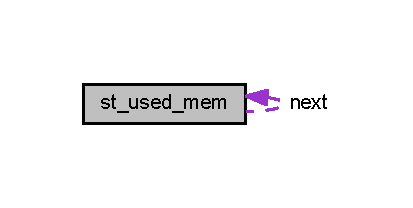
\includegraphics[width=198pt]{structst__used__mem__coll__graph}
\end{center}
\end{figure}
\subsection*{Data Fields}
\begin{DoxyCompactItemize}
\item 
struct \hyperlink{structst__used__mem}{st\+\_\+used\+\_\+mem} $\ast$ \hyperlink{structst__used__mem_af0d44c8373329563afc30a14acc810b4}{next}
\item 
unsigned int \hyperlink{structst__used__mem_ac11095c69589cce049d735d036c638f5}{left}
\item 
unsigned int \hyperlink{structst__used__mem_ab8fe1a337ad5024c34bd7b26400ce96e}{size}
\end{DoxyCompactItemize}


\subsection{Field Documentation}
\hypertarget{structst__used__mem_ac11095c69589cce049d735d036c638f5}{}\index{st\+\_\+used\+\_\+mem@{st\+\_\+used\+\_\+mem}!left@{left}}
\index{left@{left}!st\+\_\+used\+\_\+mem@{st\+\_\+used\+\_\+mem}}
\subsubsection[{left}]{\setlength{\rightskip}{0pt plus 5cm}unsigned int st\+\_\+used\+\_\+mem\+::left}\label{structst__used__mem_ac11095c69589cce049d735d036c638f5}
\hypertarget{structst__used__mem_af0d44c8373329563afc30a14acc810b4}{}\index{st\+\_\+used\+\_\+mem@{st\+\_\+used\+\_\+mem}!next@{next}}
\index{next@{next}!st\+\_\+used\+\_\+mem@{st\+\_\+used\+\_\+mem}}
\subsubsection[{next}]{\setlength{\rightskip}{0pt plus 5cm}struct {\bf st\+\_\+used\+\_\+mem}$\ast$ st\+\_\+used\+\_\+mem\+::next}\label{structst__used__mem_af0d44c8373329563afc30a14acc810b4}
\hypertarget{structst__used__mem_ab8fe1a337ad5024c34bd7b26400ce96e}{}\index{st\+\_\+used\+\_\+mem@{st\+\_\+used\+\_\+mem}!size@{size}}
\index{size@{size}!st\+\_\+used\+\_\+mem@{st\+\_\+used\+\_\+mem}}
\subsubsection[{size}]{\setlength{\rightskip}{0pt plus 5cm}unsigned int st\+\_\+used\+\_\+mem\+::size}\label{structst__used__mem_ab8fe1a337ad5024c34bd7b26400ce96e}


The documentation for this struct was generated from the following file\+:\begin{DoxyCompactItemize}
\item 
\hyperlink{my__alloc_8h}{my\+\_\+alloc.\+h}\end{DoxyCompactItemize}

\chapter{File Documentation}
\hypertarget{main_8c}{}\doxysection{main.\+c File Reference}
\label{main_8c}\index{main.c@{main.c}}
{\ttfamily \#include $<$D\+A\+V\+E.\+h$>$}\newline
{\ttfamily \#include \char`\"{}Manager\+Task.\+h\char`\"{}}\newline
{\ttfamily \#include \char`\"{}Uart\+Task.\+h\char`\"{}}\newline
{\ttfamily \#include \char`\"{}Spi\+Task.\+h\char`\"{}}\newline
{\ttfamily \#include \char`\"{}Worker1\+Task.\+h\char`\"{}}\newline
{\ttfamily \#include \char`\"{}Worker2\+Task.\+h\char`\"{}}\newline
Include dependency graph for main.\+c\+:
\nopagebreak
\begin{figure}[H]
\begin{center}
\leavevmode
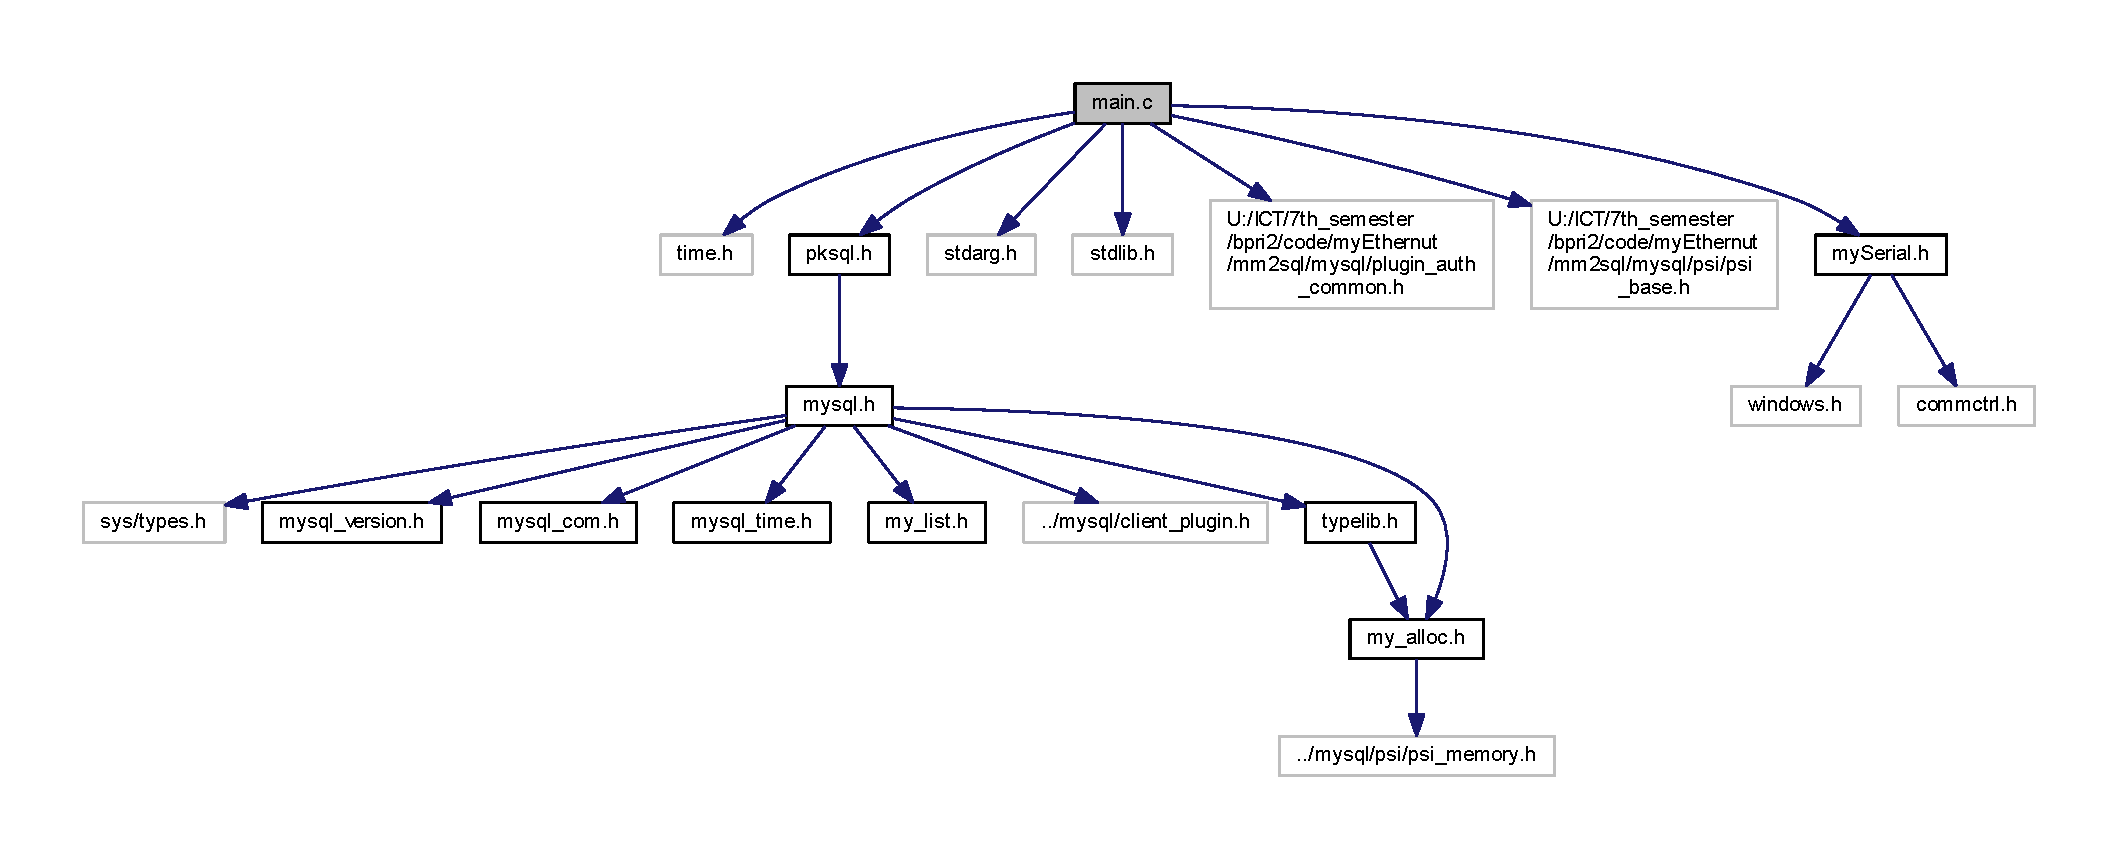
\includegraphics[width=350pt]{main_8c__incl}
\end{center}
\end{figure}
\doxysubsection*{Data Structures}
\begin{DoxyCompactItemize}
\item 
struct \mbox{\hyperlink{structparameter__struct}{parameter\+\_\+struct}}
\item 
struct \mbox{\hyperlink{struct_s_e_m_a_p_h_o_r_e___p_a_r_a_m_e_t_e_r_s}{S\+E\+M\+A\+P\+H\+O\+R\+E\+\_\+\+P\+A\+R\+A\+M\+E\+T\+E\+RS}}
\end{DoxyCompactItemize}
\doxysubsection*{Typedefs}
\begin{DoxyCompactItemize}
\item 
typedef struct \mbox{\hyperlink{structparameter__struct}{parameter\+\_\+struct}} \mbox{\hyperlink{main_8c_a4f866bc389d610b9af1569828c5cb796}{parameter\+\_\+struct\+\_\+t}}
\item 
typedef struct \mbox{\hyperlink{struct_s_e_m_a_p_h_o_r_e___p_a_r_a_m_e_t_e_r_s}{S\+E\+M\+A\+P\+H\+O\+R\+E\+\_\+\+P\+A\+R\+A\+M\+E\+T\+E\+RS}} \mbox{\hyperlink{main_8c_a8fa66a9bec224102af9be786a011d0ad}{x\+Semaphore\+Parameters\+\_\+t}}
\end{DoxyCompactItemize}
\doxysubsection*{Functions}
\begin{DoxyCompactItemize}
\item 
void \mbox{\hyperlink{main_8c_a0631242f9ef4df98c0aa08fc3477016b}{My\+L\+E\+Ds\+Toggling}} (uint8\+\_\+t tyle\+Razy)
\item 
void \mbox{\hyperlink{main_8c_a73549cfa09efe760d01971a22fd6b473}{My\+Error\+Handler}} (\mbox{\hyperlink{_generated_2_f_r_e_e_r_t_o_s_2task_8h_ae95f44d4cfeb4a599c6cc258d241cb6b}{Task\+Handle\+\_\+t}} x\+U\+A\+R\+T\+Handle)
\item 
void \mbox{\hyperlink{main_8c_a6a82a5f642a3795d49ee2a181494f472}{v\+Application\+Stack\+Overflow\+Hook}} (\mbox{\hyperlink{_model_2_a_p_p_s_2_f_r_e_e_r_t_o_s_2v4__1__2_2_templates_2_free_r_t_o_s_8h_af7cd8f53b62f0c497b442b504c30f2ec}{x\+Task\+Handle}} $\ast$px\+Task, signed char $\ast$pc\+Task\+Name)
\item 
void \mbox{\hyperlink{main_8c_a73f6aa45470ada02a5d6f3a522d8f13c}{v\+Application\+Malloc\+Failed\+Hook}} ()
\item 
void \mbox{\hyperlink{main_8c_afa643a0090e2cb938031a8ce2c46033c}{my\+Timer\+Callback}} (\mbox{\hyperlink{_model_2_a_p_p_s_2_f_r_e_e_r_t_o_s_2v4__1__2_2_templates_2_free_r_t_o_s_8h_a9fa57c444af781c3b6286f5cc9e4982d}{x\+Timer\+Handle}} px\+Timer)
\item 
int \mbox{\hyperlink{main_8c_a840291bc02cba5474a4cb46a9b9566fe}{main}} (void)
\end{DoxyCompactItemize}
\doxysubsection*{Variables}
\begin{DoxyCompactItemize}
\item 
\mbox{\hyperlink{_generated_2_f_r_e_e_r_t_o_s_2queue_8h_aaf19d499892a4ce1409326ece00f5264}{Queue\+Handle\+\_\+t}} \mbox{\hyperlink{main_8c_aa78b6121b7586233293fb6cba5e19206}{x\+Queue}} = N\+U\+LL
\item 
\mbox{\hyperlink{_model_2_a_p_p_s_2_f_r_e_e_r_t_o_s_2v4__1__2_2_templates_2_free_r_t_o_s_8h_a2b4ea2af4cc24db3cbd458722e96fa2f}{x\+Queue\+Handle}} \mbox{\hyperlink{main_8c_a1f474f190f107b23b637c1ec19339180}{Queue\+\_\+id}}
\item 
\mbox{\hyperlink{_model_2_a_p_p_s_2_f_r_e_e_r_t_o_s_2v4__1__2_2_templates_2_free_r_t_o_s_8h_a520d8cf032327581ece00e5bd8e03a75}{x\+Semaphore\+Handle}} \mbox{\hyperlink{main_8c_a518b536ed9bf3aae03f23de3ca80d69a}{notification\+\_\+semaphore}}
\item 
\mbox{\hyperlink{_model_2_a_p_p_s_2_f_r_e_e_r_t_o_s_2v4__1__2_2_templates_2_free_r_t_o_s_8h_a9fa57c444af781c3b6286f5cc9e4982d}{x\+Timer\+Handle}} \mbox{\hyperlink{main_8c_a02eac32cb5e7d9181d0197f353680c36}{Timer\+\_\+handle}}
\item 
\mbox{\hyperlink{_model_2_a_p_p_s_2_f_r_e_e_r_t_o_s_2v4__1__2_2_templates_2_free_r_t_o_s_8h_af7cd8f53b62f0c497b442b504c30f2ec}{x\+Task\+Handle}} \mbox{\hyperlink{main_8c_af9594ea483e4b18a36cc64c770a0b2a6}{U\+A\+R\+T\+Handle}} = N\+U\+LL
\item 
\mbox{\hyperlink{_model_2_a_p_p_s_2_f_r_e_e_r_t_o_s_2v4__1__2_2_templates_2_free_r_t_o_s_8h_af7cd8f53b62f0c497b442b504c30f2ec}{x\+Task\+Handle}} \mbox{\hyperlink{main_8c_aeb8570170354bebca19705854397cc75}{S\+P\+I\+Handle}} = N\+U\+LL
\item 
\mbox{\hyperlink{_model_2_a_p_p_s_2_f_r_e_e_r_t_o_s_2v4__1__2_2_templates_2_free_r_t_o_s_8h_af7cd8f53b62f0c497b442b504c30f2ec}{x\+Task\+Handle}} \mbox{\hyperlink{main_8c_a0322c8c10fc32d9da88dbb42525d11cd}{worker1\+\_\+id}}
\item 
\mbox{\hyperlink{_model_2_a_p_p_s_2_f_r_e_e_r_t_o_s_2v4__1__2_2_templates_2_free_r_t_o_s_8h_af7cd8f53b62f0c497b442b504c30f2ec}{x\+Task\+Handle}} \mbox{\hyperlink{main_8c_ae10999ad4b9b69ce410922e0a977066e}{worker2\+\_\+id}}
\end{DoxyCompactItemize}


\doxysubsection{Typedef Documentation}
\mbox{\Hypertarget{main_8c_a4f866bc389d610b9af1569828c5cb796}\label{main_8c_a4f866bc389d610b9af1569828c5cb796}} 
\index{main.c@{main.c}!parameter\_struct\_t@{parameter\_struct\_t}}
\index{parameter\_struct\_t@{parameter\_struct\_t}!main.c@{main.c}}
\doxysubsubsection{\texorpdfstring{parameter\_struct\_t}{parameter\_struct\_t}}
{\footnotesize\ttfamily typedef struct \mbox{\hyperlink{structparameter__struct}{parameter\+\_\+struct}} \mbox{\hyperlink{main_8c_a4f866bc389d610b9af1569828c5cb796}{parameter\+\_\+struct\+\_\+t}}}

\mbox{\Hypertarget{main_8c_a8fa66a9bec224102af9be786a011d0ad}\label{main_8c_a8fa66a9bec224102af9be786a011d0ad}} 
\index{main.c@{main.c}!xSemaphoreParameters\_t@{xSemaphoreParameters\_t}}
\index{xSemaphoreParameters\_t@{xSemaphoreParameters\_t}!main.c@{main.c}}
\doxysubsubsection{\texorpdfstring{xSemaphoreParameters\_t}{xSemaphoreParameters\_t}}
{\footnotesize\ttfamily typedef struct \mbox{\hyperlink{struct_s_e_m_a_p_h_o_r_e___p_a_r_a_m_e_t_e_r_s}{S\+E\+M\+A\+P\+H\+O\+R\+E\+\_\+\+P\+A\+R\+A\+M\+E\+T\+E\+RS}} \mbox{\hyperlink{main_8c_a8fa66a9bec224102af9be786a011d0ad}{x\+Semaphore\+Parameters\+\_\+t}}}



\doxysubsection{Function Documentation}
\mbox{\Hypertarget{main_8c_a840291bc02cba5474a4cb46a9b9566fe}\label{main_8c_a840291bc02cba5474a4cb46a9b9566fe}} 
\index{main.c@{main.c}!main@{main}}
\index{main@{main}!main.c@{main.c}}
\doxysubsubsection{\texorpdfstring{main()}{main()}}
{\footnotesize\ttfamily int main (\begin{DoxyParamCaption}\item[{void}]{ }\end{DoxyParamCaption})}



Definition at line 77 of file main.\+c.



References config\+M\+I\+N\+I\+M\+A\+L\+\_\+\+S\+T\+A\+C\+K\+\_\+\+S\+I\+ZE, D\+A\+V\+E\+\_\+\+Init(), D\+A\+V\+E\+\_\+\+S\+T\+A\+T\+U\+S\+\_\+\+S\+U\+C\+C\+E\+SS, Manager\+\_\+\+Task(), my\+Timer\+Callback(), pd\+T\+R\+UE, pv\+Port\+Malloc(), Queue\+\_\+id, Timer\+\_\+handle, tsk\+I\+D\+L\+E\+\_\+\+P\+R\+I\+O\+R\+I\+TY, v\+Task\+Start\+Scheduler(), worker1\+\_\+id, worker1\+\_\+task(), worker2\+\_\+id, worker2\+\_\+task(), X\+M\+C\+\_\+\+D\+E\+B\+UG, x\+Queue, x\+Timer\+Create(), and x\+Timer\+Start.

Here is the call graph for this function\+:
\nopagebreak
\begin{figure}[H]
\begin{center}
\leavevmode
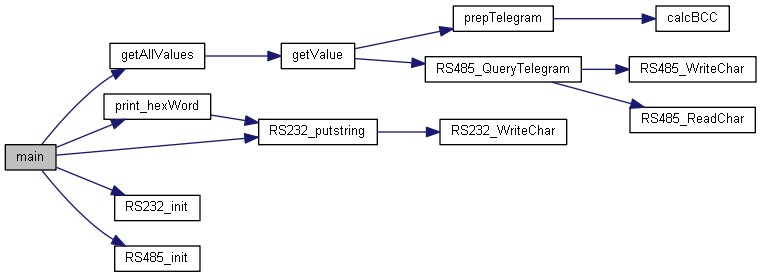
\includegraphics[width=350pt]{main_8c_a840291bc02cba5474a4cb46a9b9566fe_cgraph}
\end{center}
\end{figure}
\mbox{\Hypertarget{main_8c_a73549cfa09efe760d01971a22fd6b473}\label{main_8c_a73549cfa09efe760d01971a22fd6b473}} 
\index{main.c@{main.c}!MyErrorHandler@{MyErrorHandler}}
\index{MyErrorHandler@{MyErrorHandler}!main.c@{main.c}}
\doxysubsubsection{\texorpdfstring{MyErrorHandler()}{MyErrorHandler()}}
{\footnotesize\ttfamily void My\+Error\+Handler (\begin{DoxyParamCaption}\item[{\mbox{\hyperlink{_generated_2_f_r_e_e_r_t_o_s_2task_8h_ae95f44d4cfeb4a599c6cc258d241cb6b}{Task\+Handle\+\_\+t}}}]{x\+U\+A\+R\+T\+Handle }\end{DoxyParamCaption})}



Definition at line 42 of file main.\+c.



References My\+L\+E\+Ds\+Toggling(), pd\+M\+S\+\_\+\+T\+O\+\_\+\+T\+I\+C\+KS, v\+Task\+Delay(), and v\+Task\+Delete().

Here is the call graph for this function\+:
\nopagebreak
\begin{figure}[H]
\begin{center}
\leavevmode
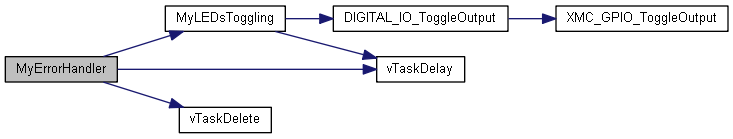
\includegraphics[width=350pt]{main_8c_a73549cfa09efe760d01971a22fd6b473_cgraph}
\end{center}
\end{figure}
\mbox{\Hypertarget{main_8c_a0631242f9ef4df98c0aa08fc3477016b}\label{main_8c_a0631242f9ef4df98c0aa08fc3477016b}} 
\index{main.c@{main.c}!MyLEDsToggling@{MyLEDsToggling}}
\index{MyLEDsToggling@{MyLEDsToggling}!main.c@{main.c}}
\doxysubsubsection{\texorpdfstring{MyLEDsToggling()}{MyLEDsToggling()}}
{\footnotesize\ttfamily void My\+L\+E\+Ds\+Toggling (\begin{DoxyParamCaption}\item[{uint8\+\_\+t}]{tyle\+Razy }\end{DoxyParamCaption})}



Definition at line 34 of file main.\+c.



References D\+I\+G\+I\+T\+A\+L\+\_\+\+I\+O\+\_\+\+Toggle\+Output(), L\+E\+D0, L\+E\+D1, and v\+Task\+Delay().



Referenced by My\+Error\+Handler(), v\+Application\+Malloc\+Failed\+Hook(), and v\+Application\+Stack\+Overflow\+Hook().

Here is the call graph for this function\+:
\nopagebreak
\begin{figure}[H]
\begin{center}
\leavevmode
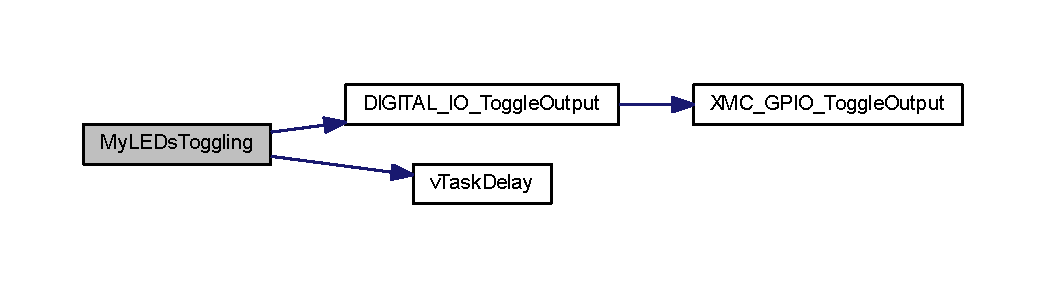
\includegraphics[width=350pt]{main_8c_a0631242f9ef4df98c0aa08fc3477016b_cgraph}
\end{center}
\end{figure}
\mbox{\Hypertarget{main_8c_afa643a0090e2cb938031a8ce2c46033c}\label{main_8c_afa643a0090e2cb938031a8ce2c46033c}} 
\index{main.c@{main.c}!myTimerCallback@{myTimerCallback}}
\index{myTimerCallback@{myTimerCallback}!main.c@{main.c}}
\doxysubsubsection{\texorpdfstring{myTimerCallback()}{myTimerCallback()}}
{\footnotesize\ttfamily void my\+Timer\+Callback (\begin{DoxyParamCaption}\item[{\mbox{\hyperlink{_model_2_a_p_p_s_2_f_r_e_e_r_t_o_s_2v4__1__2_2_templates_2_free_r_t_o_s_8h_a9fa57c444af781c3b6286f5cc9e4982d}{x\+Timer\+Handle}}}]{px\+Timer }\end{DoxyParamCaption})}



Definition at line 70 of file main.\+c.



References notification\+\_\+semaphore, and x\+Semaphore\+Give.



Referenced by main().

\mbox{\Hypertarget{main_8c_a73f6aa45470ada02a5d6f3a522d8f13c}\label{main_8c_a73f6aa45470ada02a5d6f3a522d8f13c}} 
\index{main.c@{main.c}!vApplicationMallocFailedHook@{vApplicationMallocFailedHook}}
\index{vApplicationMallocFailedHook@{vApplicationMallocFailedHook}!main.c@{main.c}}
\doxysubsubsection{\texorpdfstring{vApplicationMallocFailedHook()}{vApplicationMallocFailedHook()}}
{\footnotesize\ttfamily void v\+Application\+Malloc\+Failed\+Hook (\begin{DoxyParamCaption}{ }\end{DoxyParamCaption})}



Definition at line 63 of file main.\+c.



References My\+L\+E\+Ds\+Toggling(), pd\+M\+S\+\_\+\+T\+O\+\_\+\+T\+I\+C\+KS, and v\+Task\+Delay().



Referenced by pv\+Port\+Malloc().

Here is the call graph for this function\+:
\nopagebreak
\begin{figure}[H]
\begin{center}
\leavevmode
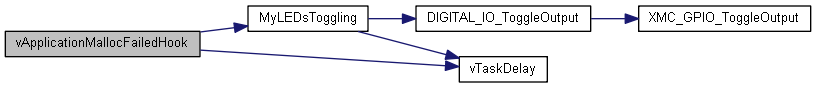
\includegraphics[width=350pt]{main_8c_a73f6aa45470ada02a5d6f3a522d8f13c_cgraph}
\end{center}
\end{figure}
\mbox{\Hypertarget{main_8c_a6a82a5f642a3795d49ee2a181494f472}\label{main_8c_a6a82a5f642a3795d49ee2a181494f472}} 
\index{main.c@{main.c}!vApplicationStackOverflowHook@{vApplicationStackOverflowHook}}
\index{vApplicationStackOverflowHook@{vApplicationStackOverflowHook}!main.c@{main.c}}
\doxysubsubsection{\texorpdfstring{vApplicationStackOverflowHook()}{vApplicationStackOverflowHook()}}
{\footnotesize\ttfamily void v\+Application\+Stack\+Overflow\+Hook (\begin{DoxyParamCaption}\item[{\mbox{\hyperlink{_model_2_a_p_p_s_2_f_r_e_e_r_t_o_s_2v4__1__2_2_templates_2_free_r_t_o_s_8h_af7cd8f53b62f0c497b442b504c30f2ec}{x\+Task\+Handle}} $\ast$}]{px\+Task,  }\item[{signed char $\ast$}]{pc\+Task\+Name }\end{DoxyParamCaption})}



Definition at line 53 of file main.\+c.



References My\+L\+E\+Ds\+Toggling(), pd\+M\+S\+\_\+\+T\+O\+\_\+\+T\+I\+C\+KS, and v\+Task\+Delay().

Here is the call graph for this function\+:
\nopagebreak
\begin{figure}[H]
\begin{center}
\leavevmode
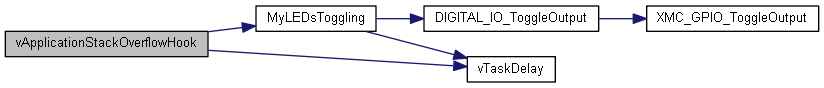
\includegraphics[width=350pt]{main_8c_a6a82a5f642a3795d49ee2a181494f472_cgraph}
\end{center}
\end{figure}


\doxysubsection{Variable Documentation}
\mbox{\Hypertarget{main_8c_a518b536ed9bf3aae03f23de3ca80d69a}\label{main_8c_a518b536ed9bf3aae03f23de3ca80d69a}} 
\index{main.c@{main.c}!notification\_semaphore@{notification\_semaphore}}
\index{notification\_semaphore@{notification\_semaphore}!main.c@{main.c}}
\doxysubsubsection{\texorpdfstring{notification\_semaphore}{notification\_semaphore}}
{\footnotesize\ttfamily \mbox{\hyperlink{_model_2_a_p_p_s_2_f_r_e_e_r_t_o_s_2v4__1__2_2_templates_2_free_r_t_o_s_8h_a520d8cf032327581ece00e5bd8e03a75}{x\+Semaphore\+Handle}} notification\+\_\+semaphore}



Definition at line 15 of file main.\+c.



Referenced by Manager\+\_\+\+Task(), and my\+Timer\+Callback().

\mbox{\Hypertarget{main_8c_a1f474f190f107b23b637c1ec19339180}\label{main_8c_a1f474f190f107b23b637c1ec19339180}} 
\index{main.c@{main.c}!Queue\_id@{Queue\_id}}
\index{Queue\_id@{Queue\_id}!main.c@{main.c}}
\doxysubsubsection{\texorpdfstring{Queue\_id}{Queue\_id}}
{\footnotesize\ttfamily \mbox{\hyperlink{_model_2_a_p_p_s_2_f_r_e_e_r_t_o_s_2v4__1__2_2_templates_2_free_r_t_o_s_8h_a2b4ea2af4cc24db3cbd458722e96fa2f}{x\+Queue\+Handle}} Queue\+\_\+id}



Definition at line 14 of file main.\+c.



Referenced by main(), Manager\+\_\+\+Task(), worker1\+\_\+task(), and worker2\+\_\+task().

\mbox{\Hypertarget{main_8c_aeb8570170354bebca19705854397cc75}\label{main_8c_aeb8570170354bebca19705854397cc75}} 
\index{main.c@{main.c}!SPIHandle@{SPIHandle}}
\index{SPIHandle@{SPIHandle}!main.c@{main.c}}
\doxysubsubsection{\texorpdfstring{SPIHandle}{SPIHandle}}
{\footnotesize\ttfamily \mbox{\hyperlink{_model_2_a_p_p_s_2_f_r_e_e_r_t_o_s_2v4__1__2_2_templates_2_free_r_t_o_s_8h_af7cd8f53b62f0c497b442b504c30f2ec}{x\+Task\+Handle}} S\+P\+I\+Handle = N\+U\+LL}



Definition at line 18 of file main.\+c.

\mbox{\Hypertarget{main_8c_a02eac32cb5e7d9181d0197f353680c36}\label{main_8c_a02eac32cb5e7d9181d0197f353680c36}} 
\index{main.c@{main.c}!Timer\_handle@{Timer\_handle}}
\index{Timer\_handle@{Timer\_handle}!main.c@{main.c}}
\doxysubsubsection{\texorpdfstring{Timer\_handle}{Timer\_handle}}
{\footnotesize\ttfamily \mbox{\hyperlink{_model_2_a_p_p_s_2_f_r_e_e_r_t_o_s_2v4__1__2_2_templates_2_free_r_t_o_s_8h_a9fa57c444af781c3b6286f5cc9e4982d}{x\+Timer\+Handle}} Timer\+\_\+handle}



Definition at line 16 of file main.\+c.



Referenced by main().

\mbox{\Hypertarget{main_8c_af9594ea483e4b18a36cc64c770a0b2a6}\label{main_8c_af9594ea483e4b18a36cc64c770a0b2a6}} 
\index{main.c@{main.c}!UARTHandle@{UARTHandle}}
\index{UARTHandle@{UARTHandle}!main.c@{main.c}}
\doxysubsubsection{\texorpdfstring{UARTHandle}{UARTHandle}}
{\footnotesize\ttfamily \mbox{\hyperlink{_model_2_a_p_p_s_2_f_r_e_e_r_t_o_s_2v4__1__2_2_templates_2_free_r_t_o_s_8h_af7cd8f53b62f0c497b442b504c30f2ec}{x\+Task\+Handle}} U\+A\+R\+T\+Handle = N\+U\+LL}



Definition at line 17 of file main.\+c.

\mbox{\Hypertarget{main_8c_a0322c8c10fc32d9da88dbb42525d11cd}\label{main_8c_a0322c8c10fc32d9da88dbb42525d11cd}} 
\index{main.c@{main.c}!worker1\_id@{worker1\_id}}
\index{worker1\_id@{worker1\_id}!main.c@{main.c}}
\doxysubsubsection{\texorpdfstring{worker1\_id}{worker1\_id}}
{\footnotesize\ttfamily \mbox{\hyperlink{_model_2_a_p_p_s_2_f_r_e_e_r_t_o_s_2v4__1__2_2_templates_2_free_r_t_o_s_8h_af7cd8f53b62f0c497b442b504c30f2ec}{x\+Task\+Handle}} worker1\+\_\+id}



Definition at line 19 of file main.\+c.



Referenced by main(), Manager\+\_\+\+Task(), and worker1\+\_\+task().

\mbox{\Hypertarget{main_8c_ae10999ad4b9b69ce410922e0a977066e}\label{main_8c_ae10999ad4b9b69ce410922e0a977066e}} 
\index{main.c@{main.c}!worker2\_id@{worker2\_id}}
\index{worker2\_id@{worker2\_id}!main.c@{main.c}}
\doxysubsubsection{\texorpdfstring{worker2\_id}{worker2\_id}}
{\footnotesize\ttfamily \mbox{\hyperlink{_model_2_a_p_p_s_2_f_r_e_e_r_t_o_s_2v4__1__2_2_templates_2_free_r_t_o_s_8h_af7cd8f53b62f0c497b442b504c30f2ec}{x\+Task\+Handle}} worker2\+\_\+id}



Definition at line 20 of file main.\+c.



Referenced by main(), Manager\+\_\+\+Task(), and worker2\+\_\+task().

\mbox{\Hypertarget{main_8c_aa78b6121b7586233293fb6cba5e19206}\label{main_8c_aa78b6121b7586233293fb6cba5e19206}} 
\index{main.c@{main.c}!xQueue@{xQueue}}
\index{xQueue@{xQueue}!main.c@{main.c}}
\doxysubsubsection{\texorpdfstring{xQueue}{xQueue}}
{\footnotesize\ttfamily \mbox{\hyperlink{_generated_2_f_r_e_e_r_t_o_s_2queue_8h_aaf19d499892a4ce1409326ece00f5264}{Queue\+Handle\+\_\+t}} x\+Queue = N\+U\+LL}



Definition at line 13 of file main.\+c.



Referenced by main(), pc\+Queue\+Get\+Name(), S\+P\+I\+\_\+\+Slave\+\_\+\+Task(), U\+A\+R\+T\+\_\+\+Task(), uc\+Queue\+Get\+Queue\+Type(), ux\+Queue\+Get\+Queue\+Number(), ux\+Queue\+Messages\+Waiting(), ux\+Queue\+Messages\+Waiting\+From\+I\+S\+R(), ux\+Queue\+Spaces\+Available(), v\+Queue\+Add\+To\+Registry(), v\+Queue\+Delete(), v\+Queue\+Set\+Queue\+Number(), v\+Queue\+Unregister\+Queue(), v\+Queue\+Wait\+For\+Message\+Restricted(), x\+Queue\+Generic\+Reset(), x\+Queue\+Generic\+Send(), x\+Queue\+Generic\+Send\+From\+I\+S\+R(), x\+Queue\+Give\+From\+I\+S\+R(), x\+Queue\+Is\+Queue\+Empty\+From\+I\+S\+R(), x\+Queue\+Is\+Queue\+Full\+From\+I\+S\+R(), x\+Queue\+Peek(), x\+Queue\+Peek\+From\+I\+S\+R(), x\+Queue\+Receive(), x\+Queue\+Receive\+From\+I\+S\+R(), and x\+Queue\+Semaphore\+Take().


\hypertarget{my__alloc_8h}{}\section{my\+\_\+alloc.\+h File Reference}
\label{my__alloc_8h}\index{my\+\_\+alloc.\+h@{my\+\_\+alloc.\+h}}
{\ttfamily \#include \char`\"{}../mysql/psi/psi\+\_\+memory.\+h\char`\"{}}\\*
Include dependency graph for my\+\_\+alloc.\+h\+:\nopagebreak
\begin{figure}[H]
\begin{center}
\leavevmode
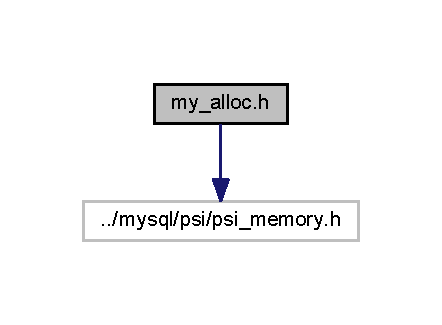
\includegraphics[width=212pt]{my__alloc_8h__incl}
\end{center}
\end{figure}
This graph shows which files directly or indirectly include this file\+:\nopagebreak
\begin{figure}[H]
\begin{center}
\leavevmode
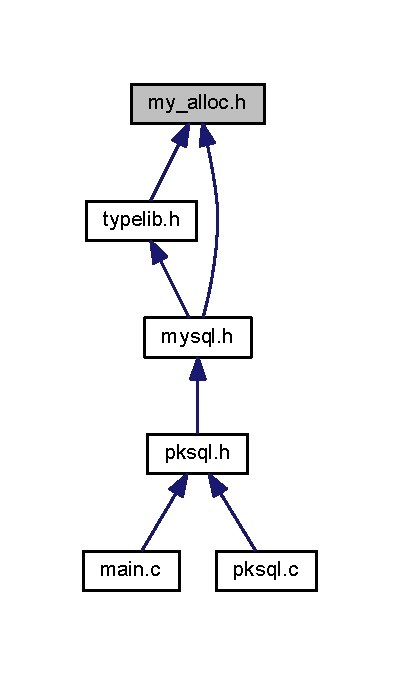
\includegraphics[width=192pt]{my__alloc_8h__dep__incl}
\end{center}
\end{figure}
\subsection*{Data Structures}
\begin{DoxyCompactItemize}
\item 
struct \hyperlink{structst__used__mem}{st\+\_\+used\+\_\+mem}
\item 
struct \hyperlink{structst__mem__root}{st\+\_\+mem\+\_\+root}
\end{DoxyCompactItemize}
\subsection*{Macros}
\begin{DoxyCompactItemize}
\item 
\#define \hyperlink{my__alloc_8h_a86cee62dcc3de4c3ca52d41583603175}{A\+L\+L\+O\+C\+\_\+\+M\+A\+X\+\_\+\+B\+L\+O\+C\+K\+\_\+\+T\+O\+\_\+\+D\+R\+O\+P}~4096
\item 
\#define \hyperlink{my__alloc_8h_a567173e2e9814210374c5351959e349b}{A\+L\+L\+O\+C\+\_\+\+M\+A\+X\+\_\+\+B\+L\+O\+C\+K\+\_\+\+U\+S\+A\+G\+E\+\_\+\+B\+E\+F\+O\+R\+E\+\_\+\+D\+R\+O\+P}~10
\end{DoxyCompactItemize}
\subsection*{Typedefs}
\begin{DoxyCompactItemize}
\item 
typedef struct \hyperlink{structst__used__mem}{st\+\_\+used\+\_\+mem} \hyperlink{my__alloc_8h_adcee356751476eb8212d707ab71a525c}{U\+S\+E\+D\+\_\+\+M\+E\+M}
\item 
typedef struct \hyperlink{structst__mem__root}{st\+\_\+mem\+\_\+root} \hyperlink{my__alloc_8h_ac59e289b254a2c5ac634ffcedda3f823}{M\+E\+M\+\_\+\+R\+O\+O\+T}
\end{DoxyCompactItemize}


\subsection{Macro Definition Documentation}
\hypertarget{my__alloc_8h_a86cee62dcc3de4c3ca52d41583603175}{}\index{my\+\_\+alloc.\+h@{my\+\_\+alloc.\+h}!A\+L\+L\+O\+C\+\_\+\+M\+A\+X\+\_\+\+B\+L\+O\+C\+K\+\_\+\+T\+O\+\_\+\+D\+R\+O\+P@{A\+L\+L\+O\+C\+\_\+\+M\+A\+X\+\_\+\+B\+L\+O\+C\+K\+\_\+\+T\+O\+\_\+\+D\+R\+O\+P}}
\index{A\+L\+L\+O\+C\+\_\+\+M\+A\+X\+\_\+\+B\+L\+O\+C\+K\+\_\+\+T\+O\+\_\+\+D\+R\+O\+P@{A\+L\+L\+O\+C\+\_\+\+M\+A\+X\+\_\+\+B\+L\+O\+C\+K\+\_\+\+T\+O\+\_\+\+D\+R\+O\+P}!my\+\_\+alloc.\+h@{my\+\_\+alloc.\+h}}
\subsubsection[{A\+L\+L\+O\+C\+\_\+\+M\+A\+X\+\_\+\+B\+L\+O\+C\+K\+\_\+\+T\+O\+\_\+\+D\+R\+O\+P}]{\setlength{\rightskip}{0pt plus 5cm}\#define A\+L\+L\+O\+C\+\_\+\+M\+A\+X\+\_\+\+B\+L\+O\+C\+K\+\_\+\+T\+O\+\_\+\+D\+R\+O\+P~4096}\label{my__alloc_8h_a86cee62dcc3de4c3ca52d41583603175}
\hypertarget{my__alloc_8h_a567173e2e9814210374c5351959e349b}{}\index{my\+\_\+alloc.\+h@{my\+\_\+alloc.\+h}!A\+L\+L\+O\+C\+\_\+\+M\+A\+X\+\_\+\+B\+L\+O\+C\+K\+\_\+\+U\+S\+A\+G\+E\+\_\+\+B\+E\+F\+O\+R\+E\+\_\+\+D\+R\+O\+P@{A\+L\+L\+O\+C\+\_\+\+M\+A\+X\+\_\+\+B\+L\+O\+C\+K\+\_\+\+U\+S\+A\+G\+E\+\_\+\+B\+E\+F\+O\+R\+E\+\_\+\+D\+R\+O\+P}}
\index{A\+L\+L\+O\+C\+\_\+\+M\+A\+X\+\_\+\+B\+L\+O\+C\+K\+\_\+\+U\+S\+A\+G\+E\+\_\+\+B\+E\+F\+O\+R\+E\+\_\+\+D\+R\+O\+P@{A\+L\+L\+O\+C\+\_\+\+M\+A\+X\+\_\+\+B\+L\+O\+C\+K\+\_\+\+U\+S\+A\+G\+E\+\_\+\+B\+E\+F\+O\+R\+E\+\_\+\+D\+R\+O\+P}!my\+\_\+alloc.\+h@{my\+\_\+alloc.\+h}}
\subsubsection[{A\+L\+L\+O\+C\+\_\+\+M\+A\+X\+\_\+\+B\+L\+O\+C\+K\+\_\+\+U\+S\+A\+G\+E\+\_\+\+B\+E\+F\+O\+R\+E\+\_\+\+D\+R\+O\+P}]{\setlength{\rightskip}{0pt plus 5cm}\#define A\+L\+L\+O\+C\+\_\+\+M\+A\+X\+\_\+\+B\+L\+O\+C\+K\+\_\+\+U\+S\+A\+G\+E\+\_\+\+B\+E\+F\+O\+R\+E\+\_\+\+D\+R\+O\+P~10}\label{my__alloc_8h_a567173e2e9814210374c5351959e349b}


\subsection{Typedef Documentation}
\hypertarget{my__alloc_8h_ac59e289b254a2c5ac634ffcedda3f823}{}\index{my\+\_\+alloc.\+h@{my\+\_\+alloc.\+h}!M\+E\+M\+\_\+\+R\+O\+O\+T@{M\+E\+M\+\_\+\+R\+O\+O\+T}}
\index{M\+E\+M\+\_\+\+R\+O\+O\+T@{M\+E\+M\+\_\+\+R\+O\+O\+T}!my\+\_\+alloc.\+h@{my\+\_\+alloc.\+h}}
\subsubsection[{M\+E\+M\+\_\+\+R\+O\+O\+T}]{\setlength{\rightskip}{0pt plus 5cm}typedef struct {\bf st\+\_\+mem\+\_\+root}  {\bf M\+E\+M\+\_\+\+R\+O\+O\+T}}\label{my__alloc_8h_ac59e289b254a2c5ac634ffcedda3f823}
\hypertarget{my__alloc_8h_adcee356751476eb8212d707ab71a525c}{}\index{my\+\_\+alloc.\+h@{my\+\_\+alloc.\+h}!U\+S\+E\+D\+\_\+\+M\+E\+M@{U\+S\+E\+D\+\_\+\+M\+E\+M}}
\index{U\+S\+E\+D\+\_\+\+M\+E\+M@{U\+S\+E\+D\+\_\+\+M\+E\+M}!my\+\_\+alloc.\+h@{my\+\_\+alloc.\+h}}
\subsubsection[{U\+S\+E\+D\+\_\+\+M\+E\+M}]{\setlength{\rightskip}{0pt plus 5cm}typedef struct {\bf st\+\_\+used\+\_\+mem}  {\bf U\+S\+E\+D\+\_\+\+M\+E\+M}}\label{my__alloc_8h_adcee356751476eb8212d707ab71a525c}

\hypertarget{my__list_8h}{}\section{my\+\_\+list.\+h File Reference}
\label{my__list_8h}\index{my\+\_\+list.\+h@{my\+\_\+list.\+h}}
This graph shows which files directly or indirectly include this file\+:\nopagebreak
\begin{figure}[H]
\begin{center}
\leavevmode
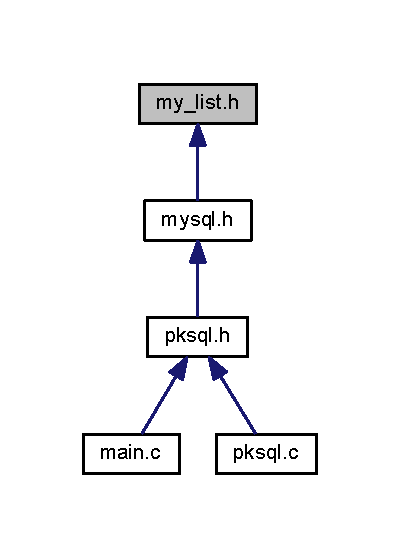
\includegraphics[width=192pt]{my__list_8h__dep__incl}
\end{center}
\end{figure}
\subsection*{Data Structures}
\begin{DoxyCompactItemize}
\item 
struct \hyperlink{structst__list}{st\+\_\+list}
\end{DoxyCompactItemize}
\subsection*{Macros}
\begin{DoxyCompactItemize}
\item 
\#define \hyperlink{my__list_8h_a4dedcce48eb31eb34f43d01a117b0a09}{list\+\_\+rest}(a)~((a)-\/$>$next)
\item 
\#define \hyperlink{my__list_8h_a4fd4bea6adf6b20816eeb88750760131}{list\+\_\+push}(a,  b)~(a)=\hyperlink{my__list_8h_aeac1351e9825db9b491f3c6a075ce9eb}{list\+\_\+cons}((b),(a))
\item 
\#define \hyperlink{my__list_8h_a6ce34cc98ba3c74574ef88670b7768f1}{list\+\_\+pop}(A)~\{\hyperlink{my__list_8h_ab2a1c5fd766481fe9ec169b9fdca184e}{L\+I\+S\+T} $\ast$old=(A); (A)=\hyperlink{my__list_8h_a11b570dab91ab5f568bc41541d297e03}{list\+\_\+delete}(old,old); my\+\_\+free(old); \}
\end{DoxyCompactItemize}
\subsection*{Typedefs}
\begin{DoxyCompactItemize}
\item 
typedef struct \hyperlink{structst__list}{st\+\_\+list} \hyperlink{my__list_8h_ab2a1c5fd766481fe9ec169b9fdca184e}{L\+I\+S\+T}
\item 
typedef int($\ast$ \hyperlink{my__list_8h_aeca49f9affc13a8284e287e82a578f1f}{list\+\_\+walk\+\_\+action}) (void $\ast$, void $\ast$)
\end{DoxyCompactItemize}
\subsection*{Functions}
\begin{DoxyCompactItemize}
\item 
\hyperlink{my__list_8h_ab2a1c5fd766481fe9ec169b9fdca184e}{L\+I\+S\+T} $\ast$ \hyperlink{my__list_8h_aed18cad350263cec89453b7afd548c7a}{list\+\_\+add} (\hyperlink{my__list_8h_ab2a1c5fd766481fe9ec169b9fdca184e}{L\+I\+S\+T} $\ast$root, \hyperlink{my__list_8h_ab2a1c5fd766481fe9ec169b9fdca184e}{L\+I\+S\+T} $\ast$element)
\item 
\hyperlink{my__list_8h_ab2a1c5fd766481fe9ec169b9fdca184e}{L\+I\+S\+T} $\ast$ \hyperlink{my__list_8h_a11b570dab91ab5f568bc41541d297e03}{list\+\_\+delete} (\hyperlink{my__list_8h_ab2a1c5fd766481fe9ec169b9fdca184e}{L\+I\+S\+T} $\ast$root, \hyperlink{my__list_8h_ab2a1c5fd766481fe9ec169b9fdca184e}{L\+I\+S\+T} $\ast$element)
\item 
\hyperlink{my__list_8h_ab2a1c5fd766481fe9ec169b9fdca184e}{L\+I\+S\+T} $\ast$ \hyperlink{my__list_8h_aeac1351e9825db9b491f3c6a075ce9eb}{list\+\_\+cons} (void $\ast$data, \hyperlink{my__list_8h_ab2a1c5fd766481fe9ec169b9fdca184e}{L\+I\+S\+T} $\ast$root)
\item 
\hyperlink{my__list_8h_ab2a1c5fd766481fe9ec169b9fdca184e}{L\+I\+S\+T} $\ast$ \hyperlink{my__list_8h_ac40e1e83b450caa91b1ba5dfe69fb419}{list\+\_\+reverse} (\hyperlink{my__list_8h_ab2a1c5fd766481fe9ec169b9fdca184e}{L\+I\+S\+T} $\ast$root)
\item 
void \hyperlink{my__list_8h_a911795309fc233e103bd6a3da13ad5fa}{list\+\_\+free} (\hyperlink{my__list_8h_ab2a1c5fd766481fe9ec169b9fdca184e}{L\+I\+S\+T} $\ast$root, unsigned int free\+\_\+data)
\item 
unsigned int \hyperlink{my__list_8h_a0e3e82b73e930fcfe7d8e4e50b604ec1}{list\+\_\+length} (\hyperlink{my__list_8h_ab2a1c5fd766481fe9ec169b9fdca184e}{L\+I\+S\+T} $\ast$)
\item 
int \hyperlink{my__list_8h_ae1cb86e2197f52f83cd2bd7acdbf51b4}{list\+\_\+walk} (\hyperlink{my__list_8h_ab2a1c5fd766481fe9ec169b9fdca184e}{L\+I\+S\+T} $\ast$, \hyperlink{my__list_8h_aeca49f9affc13a8284e287e82a578f1f}{list\+\_\+walk\+\_\+action} action, unsigned char $\ast$argument)
\end{DoxyCompactItemize}


\subsection{Macro Definition Documentation}
\hypertarget{my__list_8h_a6ce34cc98ba3c74574ef88670b7768f1}{}\index{my\+\_\+list.\+h@{my\+\_\+list.\+h}!list\+\_\+pop@{list\+\_\+pop}}
\index{list\+\_\+pop@{list\+\_\+pop}!my\+\_\+list.\+h@{my\+\_\+list.\+h}}
\subsubsection[{list\+\_\+pop}]{\setlength{\rightskip}{0pt plus 5cm}\#define list\+\_\+pop(
\begin{DoxyParamCaption}
\item[{}]{A}
\end{DoxyParamCaption}
)~\{{\bf L\+I\+S\+T} $\ast$old=(A); (A)={\bf list\+\_\+delete}(old,old); my\+\_\+free(old); \}}\label{my__list_8h_a6ce34cc98ba3c74574ef88670b7768f1}
\hypertarget{my__list_8h_a4fd4bea6adf6b20816eeb88750760131}{}\index{my\+\_\+list.\+h@{my\+\_\+list.\+h}!list\+\_\+push@{list\+\_\+push}}
\index{list\+\_\+push@{list\+\_\+push}!my\+\_\+list.\+h@{my\+\_\+list.\+h}}
\subsubsection[{list\+\_\+push}]{\setlength{\rightskip}{0pt plus 5cm}\#define list\+\_\+push(
\begin{DoxyParamCaption}
\item[{}]{a, }
\item[{}]{b}
\end{DoxyParamCaption}
)~(a)={\bf list\+\_\+cons}((b),(a))}\label{my__list_8h_a4fd4bea6adf6b20816eeb88750760131}
\hypertarget{my__list_8h_a4dedcce48eb31eb34f43d01a117b0a09}{}\index{my\+\_\+list.\+h@{my\+\_\+list.\+h}!list\+\_\+rest@{list\+\_\+rest}}
\index{list\+\_\+rest@{list\+\_\+rest}!my\+\_\+list.\+h@{my\+\_\+list.\+h}}
\subsubsection[{list\+\_\+rest}]{\setlength{\rightskip}{0pt plus 5cm}\#define list\+\_\+rest(
\begin{DoxyParamCaption}
\item[{}]{a}
\end{DoxyParamCaption}
)~((a)-\/$>$next)}\label{my__list_8h_a4dedcce48eb31eb34f43d01a117b0a09}


\subsection{Typedef Documentation}
\hypertarget{my__list_8h_ab2a1c5fd766481fe9ec169b9fdca184e}{}\index{my\+\_\+list.\+h@{my\+\_\+list.\+h}!L\+I\+S\+T@{L\+I\+S\+T}}
\index{L\+I\+S\+T@{L\+I\+S\+T}!my\+\_\+list.\+h@{my\+\_\+list.\+h}}
\subsubsection[{L\+I\+S\+T}]{\setlength{\rightskip}{0pt plus 5cm}typedef struct {\bf st\+\_\+list}  {\bf L\+I\+S\+T}}\label{my__list_8h_ab2a1c5fd766481fe9ec169b9fdca184e}
\hypertarget{my__list_8h_aeca49f9affc13a8284e287e82a578f1f}{}\index{my\+\_\+list.\+h@{my\+\_\+list.\+h}!list\+\_\+walk\+\_\+action@{list\+\_\+walk\+\_\+action}}
\index{list\+\_\+walk\+\_\+action@{list\+\_\+walk\+\_\+action}!my\+\_\+list.\+h@{my\+\_\+list.\+h}}
\subsubsection[{list\+\_\+walk\+\_\+action}]{\setlength{\rightskip}{0pt plus 5cm}typedef int($\ast$ list\+\_\+walk\+\_\+action) (void $\ast$, void $\ast$)}\label{my__list_8h_aeca49f9affc13a8284e287e82a578f1f}


\subsection{Function Documentation}
\hypertarget{my__list_8h_aed18cad350263cec89453b7afd548c7a}{}\index{my\+\_\+list.\+h@{my\+\_\+list.\+h}!list\+\_\+add@{list\+\_\+add}}
\index{list\+\_\+add@{list\+\_\+add}!my\+\_\+list.\+h@{my\+\_\+list.\+h}}
\subsubsection[{list\+\_\+add(\+L\+I\+S\+T $\ast$root, L\+I\+S\+T $\ast$element)}]{\setlength{\rightskip}{0pt plus 5cm}{\bf L\+I\+S\+T}$\ast$ list\+\_\+add (
\begin{DoxyParamCaption}
\item[{{\bf L\+I\+S\+T} $\ast$}]{root, }
\item[{{\bf L\+I\+S\+T} $\ast$}]{element}
\end{DoxyParamCaption}
)}\label{my__list_8h_aed18cad350263cec89453b7afd548c7a}
\hypertarget{my__list_8h_aeac1351e9825db9b491f3c6a075ce9eb}{}\index{my\+\_\+list.\+h@{my\+\_\+list.\+h}!list\+\_\+cons@{list\+\_\+cons}}
\index{list\+\_\+cons@{list\+\_\+cons}!my\+\_\+list.\+h@{my\+\_\+list.\+h}}
\subsubsection[{list\+\_\+cons(void $\ast$data, L\+I\+S\+T $\ast$root)}]{\setlength{\rightskip}{0pt plus 5cm}{\bf L\+I\+S\+T}$\ast$ list\+\_\+cons (
\begin{DoxyParamCaption}
\item[{void $\ast$}]{data, }
\item[{{\bf L\+I\+S\+T} $\ast$}]{root}
\end{DoxyParamCaption}
)}\label{my__list_8h_aeac1351e9825db9b491f3c6a075ce9eb}
\hypertarget{my__list_8h_a11b570dab91ab5f568bc41541d297e03}{}\index{my\+\_\+list.\+h@{my\+\_\+list.\+h}!list\+\_\+delete@{list\+\_\+delete}}
\index{list\+\_\+delete@{list\+\_\+delete}!my\+\_\+list.\+h@{my\+\_\+list.\+h}}
\subsubsection[{list\+\_\+delete(\+L\+I\+S\+T $\ast$root, L\+I\+S\+T $\ast$element)}]{\setlength{\rightskip}{0pt plus 5cm}{\bf L\+I\+S\+T}$\ast$ list\+\_\+delete (
\begin{DoxyParamCaption}
\item[{{\bf L\+I\+S\+T} $\ast$}]{root, }
\item[{{\bf L\+I\+S\+T} $\ast$}]{element}
\end{DoxyParamCaption}
)}\label{my__list_8h_a11b570dab91ab5f568bc41541d297e03}
\hypertarget{my__list_8h_a911795309fc233e103bd6a3da13ad5fa}{}\index{my\+\_\+list.\+h@{my\+\_\+list.\+h}!list\+\_\+free@{list\+\_\+free}}
\index{list\+\_\+free@{list\+\_\+free}!my\+\_\+list.\+h@{my\+\_\+list.\+h}}
\subsubsection[{list\+\_\+free(\+L\+I\+S\+T $\ast$root, unsigned int free\+\_\+data)}]{\setlength{\rightskip}{0pt plus 5cm}void list\+\_\+free (
\begin{DoxyParamCaption}
\item[{{\bf L\+I\+S\+T} $\ast$}]{root, }
\item[{unsigned int}]{free\+\_\+data}
\end{DoxyParamCaption}
)}\label{my__list_8h_a911795309fc233e103bd6a3da13ad5fa}
\hypertarget{my__list_8h_a0e3e82b73e930fcfe7d8e4e50b604ec1}{}\index{my\+\_\+list.\+h@{my\+\_\+list.\+h}!list\+\_\+length@{list\+\_\+length}}
\index{list\+\_\+length@{list\+\_\+length}!my\+\_\+list.\+h@{my\+\_\+list.\+h}}
\subsubsection[{list\+\_\+length(\+L\+I\+S\+T $\ast$)}]{\setlength{\rightskip}{0pt plus 5cm}unsigned int list\+\_\+length (
\begin{DoxyParamCaption}
\item[{{\bf L\+I\+S\+T} $\ast$}]{}
\end{DoxyParamCaption}
)}\label{my__list_8h_a0e3e82b73e930fcfe7d8e4e50b604ec1}
\hypertarget{my__list_8h_ac40e1e83b450caa91b1ba5dfe69fb419}{}\index{my\+\_\+list.\+h@{my\+\_\+list.\+h}!list\+\_\+reverse@{list\+\_\+reverse}}
\index{list\+\_\+reverse@{list\+\_\+reverse}!my\+\_\+list.\+h@{my\+\_\+list.\+h}}
\subsubsection[{list\+\_\+reverse(\+L\+I\+S\+T $\ast$root)}]{\setlength{\rightskip}{0pt plus 5cm}{\bf L\+I\+S\+T}$\ast$ list\+\_\+reverse (
\begin{DoxyParamCaption}
\item[{{\bf L\+I\+S\+T} $\ast$}]{root}
\end{DoxyParamCaption}
)}\label{my__list_8h_ac40e1e83b450caa91b1ba5dfe69fb419}
\hypertarget{my__list_8h_ae1cb86e2197f52f83cd2bd7acdbf51b4}{}\index{my\+\_\+list.\+h@{my\+\_\+list.\+h}!list\+\_\+walk@{list\+\_\+walk}}
\index{list\+\_\+walk@{list\+\_\+walk}!my\+\_\+list.\+h@{my\+\_\+list.\+h}}
\subsubsection[{list\+\_\+walk(\+L\+I\+S\+T $\ast$, list\+\_\+walk\+\_\+action action, unsigned char $\ast$argument)}]{\setlength{\rightskip}{0pt plus 5cm}int list\+\_\+walk (
\begin{DoxyParamCaption}
\item[{{\bf L\+I\+S\+T} $\ast$}]{, }
\item[{{\bf list\+\_\+walk\+\_\+action}}]{action, }
\item[{unsigned char $\ast$}]{argument}
\end{DoxyParamCaption}
)}\label{my__list_8h_ae1cb86e2197f52f83cd2bd7acdbf51b4}

\hypertarget{my_serial_8c}{}\section{my\+Serial.\+c File Reference}
\label{my_serial_8c}\index{my\+Serial.\+c@{my\+Serial.\+c}}
{\ttfamily \#include \char`\"{}my\+Serial.\+h\char`\"{}}\\*
Include dependency graph for my\+Serial.\+c\+:\nopagebreak
\begin{figure}[H]
\begin{center}
\leavevmode
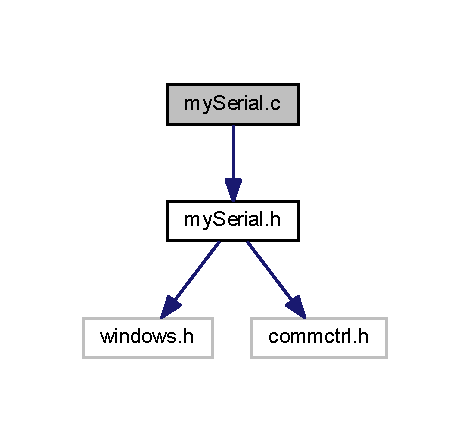
\includegraphics[width=226pt]{my_serial_8c__incl}
\end{center}
\end{figure}
\subsection*{Functions}
\begin{DoxyCompactItemize}
\item 
static C\+H\+A\+R $\ast$ \hyperlink{my_serial_8c_a8e6d0108c2d5dadf8b849a730dcd7c11}{get\+Last\+Error\+Text} (C\+H\+A\+R $\ast$p\+Buf, U\+L\+O\+N\+G buf\+Size)
\item 
B\+O\+O\+L \hyperlink{my_serial_8c_a2642c74dbe4f4d6d391253ce55b4ad02}{init\+Serial} (C\+H\+A\+R $\ast$serial\+Port)
\end{DoxyCompactItemize}


\subsection{Function Documentation}
\hypertarget{my_serial_8c_a8e6d0108c2d5dadf8b849a730dcd7c11}{}\index{my\+Serial.\+c@{my\+Serial.\+c}!get\+Last\+Error\+Text@{get\+Last\+Error\+Text}}
\index{get\+Last\+Error\+Text@{get\+Last\+Error\+Text}!my\+Serial.\+c@{my\+Serial.\+c}}
\subsubsection[{get\+Last\+Error\+Text(\+C\+H\+A\+R $\ast$p\+Buf, U\+L\+O\+N\+G buf\+Size)}]{\setlength{\rightskip}{0pt plus 5cm}static C\+H\+A\+R$\ast$ get\+Last\+Error\+Text (
\begin{DoxyParamCaption}
\item[{C\+H\+A\+R $\ast$}]{p\+Buf, }
\item[{U\+L\+O\+N\+G}]{buf\+Size}
\end{DoxyParamCaption}
)\hspace{0.3cm}{\ttfamily [static]}}\label{my_serial_8c_a8e6d0108c2d5dadf8b849a730dcd7c11}
\hypertarget{my_serial_8c_a2642c74dbe4f4d6d391253ce55b4ad02}{}\index{my\+Serial.\+c@{my\+Serial.\+c}!init\+Serial@{init\+Serial}}
\index{init\+Serial@{init\+Serial}!my\+Serial.\+c@{my\+Serial.\+c}}
\subsubsection[{init\+Serial(\+C\+H\+A\+R $\ast$serial\+Port)}]{\setlength{\rightskip}{0pt plus 5cm}B\+O\+O\+L init\+Serial (
\begin{DoxyParamCaption}
\item[{C\+H\+A\+R $\ast$}]{serial\+Port}
\end{DoxyParamCaption}
)}\label{my_serial_8c_a2642c74dbe4f4d6d391253ce55b4ad02}


Here is the call graph for this function\+:\nopagebreak
\begin{figure}[H]
\begin{center}
\leavevmode
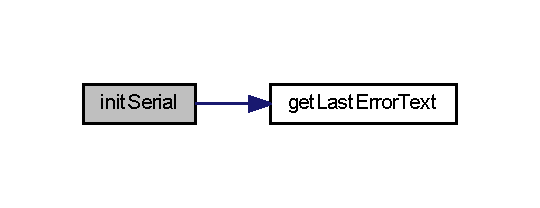
\includegraphics[width=259pt]{my_serial_8c_a2642c74dbe4f4d6d391253ce55b4ad02_cgraph}
\end{center}
\end{figure}



\hypertarget{my_serial_8h}{}\section{my\+Serial.\+h File Reference}
\label{my_serial_8h}\index{my\+Serial.\+h@{my\+Serial.\+h}}
{\ttfamily \#include $<$windows.\+h$>$}\\*
{\ttfamily \#include $<$commctrl.\+h$>$}\\*
Include dependency graph for my\+Serial.\+h\+:\nopagebreak
\begin{figure}[H]
\begin{center}
\leavevmode
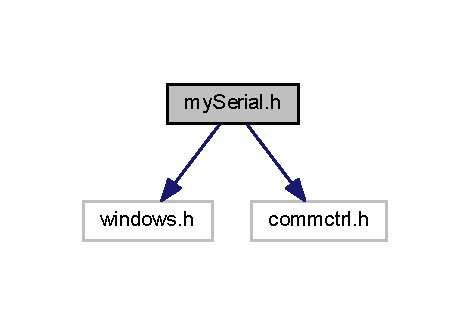
\includegraphics[width=226pt]{my_serial_8h__incl}
\end{center}
\end{figure}
This graph shows which files directly or indirectly include this file\+:\nopagebreak
\begin{figure}[H]
\begin{center}
\leavevmode
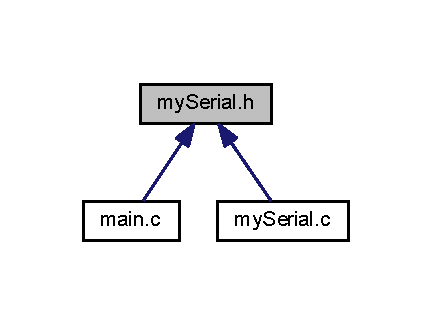
\includegraphics[width=208pt]{my_serial_8h__dep__incl}
\end{center}
\end{figure}
\subsection*{Macros}
\begin{DoxyCompactItemize}
\item 
\#define \hyperlink{my_serial_8h_a1893efb255dff8609e38157a55f8d907}{C\+O\+M\+P\+O\+R\+T}~\char`\"{}C\+O\+M1\char`\"{}
\end{DoxyCompactItemize}
\subsection*{Functions}
\begin{DoxyCompactItemize}
\item 
static C\+H\+A\+R $\ast$ \hyperlink{my_serial_8h_a8e6d0108c2d5dadf8b849a730dcd7c11}{get\+Last\+Error\+Text} (C\+H\+A\+R $\ast$p\+Buf, U\+L\+O\+N\+G buf\+Size)
\item 
B\+O\+O\+L \hyperlink{my_serial_8h_a2642c74dbe4f4d6d391253ce55b4ad02}{init\+Serial} (C\+H\+A\+R $\ast$serial\+Port)
\end{DoxyCompactItemize}
\subsection*{Variables}
\begin{DoxyCompactItemize}
\item 
H\+A\+N\+D\+L\+E \hyperlink{my_serial_8h_a1401439da773b4fec38026649db33fad}{com\+Port}
\end{DoxyCompactItemize}


\subsection{Macro Definition Documentation}
\hypertarget{my_serial_8h_a1893efb255dff8609e38157a55f8d907}{}\index{my\+Serial.\+h@{my\+Serial.\+h}!C\+O\+M\+P\+O\+R\+T@{C\+O\+M\+P\+O\+R\+T}}
\index{C\+O\+M\+P\+O\+R\+T@{C\+O\+M\+P\+O\+R\+T}!my\+Serial.\+h@{my\+Serial.\+h}}
\subsubsection[{C\+O\+M\+P\+O\+R\+T}]{\setlength{\rightskip}{0pt plus 5cm}\#define C\+O\+M\+P\+O\+R\+T~\char`\"{}C\+O\+M1\char`\"{}}\label{my_serial_8h_a1893efb255dff8609e38157a55f8d907}


\subsection{Function Documentation}
\hypertarget{my_serial_8h_a8e6d0108c2d5dadf8b849a730dcd7c11}{}\index{my\+Serial.\+h@{my\+Serial.\+h}!get\+Last\+Error\+Text@{get\+Last\+Error\+Text}}
\index{get\+Last\+Error\+Text@{get\+Last\+Error\+Text}!my\+Serial.\+h@{my\+Serial.\+h}}
\subsubsection[{get\+Last\+Error\+Text(\+C\+H\+A\+R $\ast$p\+Buf, U\+L\+O\+N\+G buf\+Size)}]{\setlength{\rightskip}{0pt plus 5cm}static C\+H\+A\+R$\ast$ get\+Last\+Error\+Text (
\begin{DoxyParamCaption}
\item[{C\+H\+A\+R $\ast$}]{p\+Buf, }
\item[{U\+L\+O\+N\+G}]{buf\+Size}
\end{DoxyParamCaption}
)\hspace{0.3cm}{\ttfamily [static]}}\label{my_serial_8h_a8e6d0108c2d5dadf8b849a730dcd7c11}
\hypertarget{my_serial_8h_a2642c74dbe4f4d6d391253ce55b4ad02}{}\index{my\+Serial.\+h@{my\+Serial.\+h}!init\+Serial@{init\+Serial}}
\index{init\+Serial@{init\+Serial}!my\+Serial.\+h@{my\+Serial.\+h}}
\subsubsection[{init\+Serial(\+C\+H\+A\+R $\ast$serial\+Port)}]{\setlength{\rightskip}{0pt plus 5cm}B\+O\+O\+L init\+Serial (
\begin{DoxyParamCaption}
\item[{C\+H\+A\+R $\ast$}]{serial\+Port}
\end{DoxyParamCaption}
)}\label{my_serial_8h_a2642c74dbe4f4d6d391253ce55b4ad02}


Here is the call graph for this function\+:\nopagebreak
\begin{figure}[H]
\begin{center}
\leavevmode
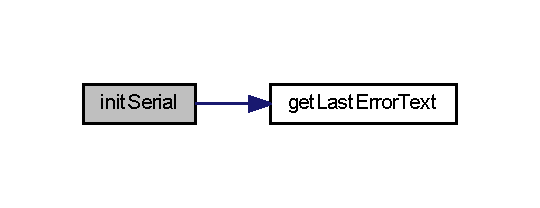
\includegraphics[width=259pt]{my_serial_8h_a2642c74dbe4f4d6d391253ce55b4ad02_cgraph}
\end{center}
\end{figure}




\subsection{Variable Documentation}
\hypertarget{my_serial_8h_a1401439da773b4fec38026649db33fad}{}\index{my\+Serial.\+h@{my\+Serial.\+h}!com\+Port@{com\+Port}}
\index{com\+Port@{com\+Port}!my\+Serial.\+h@{my\+Serial.\+h}}
\subsubsection[{com\+Port}]{\setlength{\rightskip}{0pt plus 5cm}H\+A\+N\+D\+L\+E com\+Port}\label{my_serial_8h_a1401439da773b4fec38026649db33fad}

\hypertarget{mysql_8h}{}\section{mysql.\+h File Reference}
\label{mysql_8h}\index{mysql.\+h@{mysql.\+h}}
{\ttfamily \#include $<$sys/types.\+h$>$}\\*
{\ttfamily \#include \char`\"{}mysql\+\_\+version.\+h\char`\"{}}\\*
{\ttfamily \#include \char`\"{}mysql\+\_\+com.\+h\char`\"{}}\\*
{\ttfamily \#include \char`\"{}mysql\+\_\+time.\+h\char`\"{}}\\*
{\ttfamily \#include \char`\"{}my\+\_\+list.\+h\char`\"{}}\\*
{\ttfamily \#include \char`\"{}../mysql/client\+\_\+plugin.\+h\char`\"{}}\\*
{\ttfamily \#include \char`\"{}typelib.\+h\char`\"{}}\\*
{\ttfamily \#include \char`\"{}my\+\_\+alloc.\+h\char`\"{}}\\*
Include dependency graph for mysql.\+h\+:\nopagebreak
\begin{figure}[H]
\begin{center}
\leavevmode
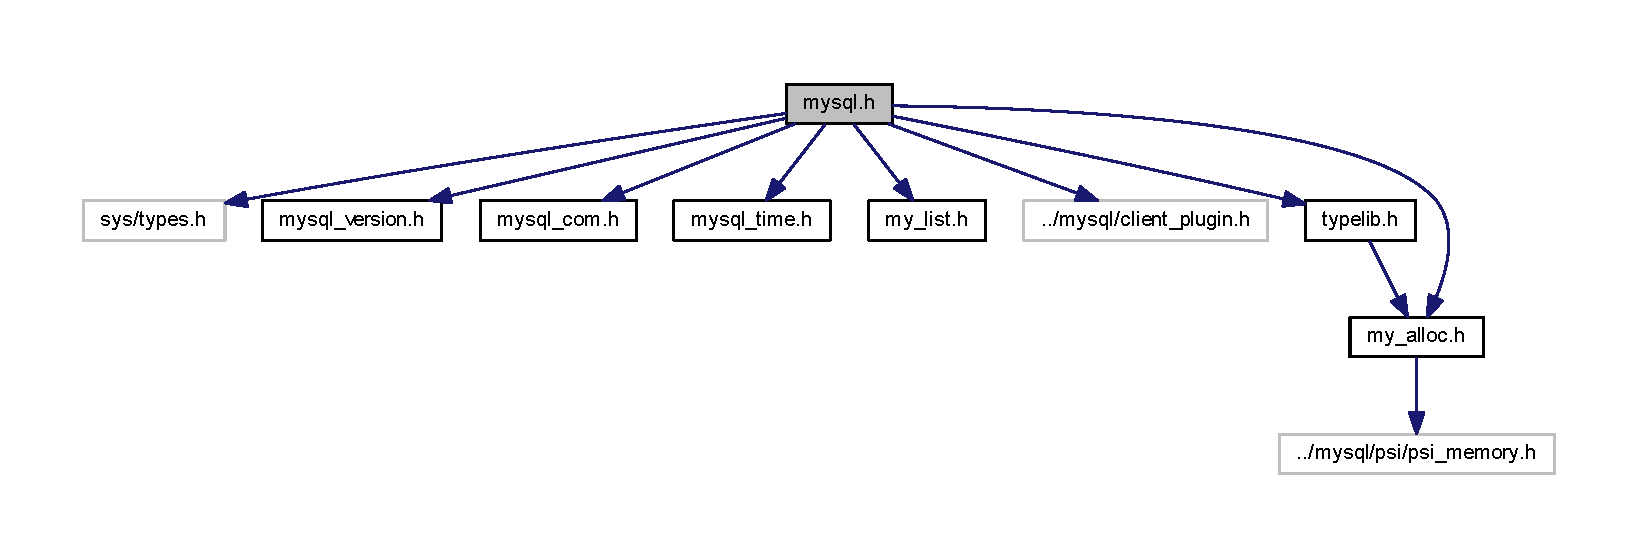
\includegraphics[width=350pt]{mysql_8h__incl}
\end{center}
\end{figure}
This graph shows which files directly or indirectly include this file\+:\nopagebreak
\begin{figure}[H]
\begin{center}
\leavevmode
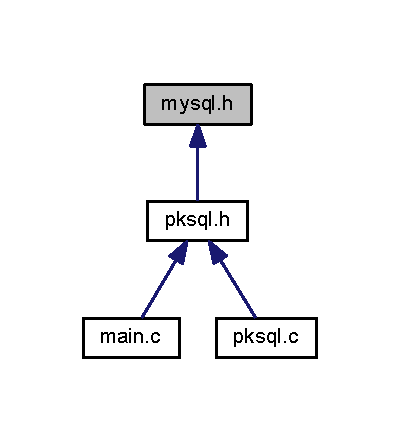
\includegraphics[width=192pt]{mysql_8h__dep__incl}
\end{center}
\end{figure}
\subsection*{Data Structures}
\begin{DoxyCompactItemize}
\item 
struct \hyperlink{structst__mysql__field}{st\+\_\+mysql\+\_\+field}
\item 
struct \hyperlink{structst__mysql__rows}{st\+\_\+mysql\+\_\+rows}
\item 
struct \hyperlink{structst__mysql__data}{st\+\_\+mysql\+\_\+data}
\item 
struct \hyperlink{structst__mysql__options}{st\+\_\+mysql\+\_\+options}
\item 
struct \hyperlink{structcharacter__set}{character\+\_\+set}
\item 
struct \hyperlink{structst__mysql}{st\+\_\+mysql}
\item 
struct \hyperlink{structst__mysql__res}{st\+\_\+mysql\+\_\+res}
\item 
struct \hyperlink{structst__mysql__parameters}{st\+\_\+mysql\+\_\+parameters}
\item 
struct \hyperlink{structst__mysql__bind}{st\+\_\+mysql\+\_\+bind}
\item 
struct \hyperlink{structst__mysql__stmt}{st\+\_\+mysql\+\_\+stmt}
\end{DoxyCompactItemize}
\subsection*{Macros}
\begin{DoxyCompactItemize}
\item 
\#define \hyperlink{mysql_8h_a446cf449a6234c9b177309d5ba0852c0}{S\+T\+D\+C\+A\+L\+L}
\item 
\#define \hyperlink{mysql_8h_a2a9336a51b002fb5ff147e574d6434be}{C\+L\+I\+E\+N\+T\+\_\+\+N\+E\+T\+\_\+\+R\+E\+A\+D\+\_\+\+T\+I\+M\+E\+O\+U\+T}~365$\ast$24$\ast$3600	/$\ast$ Timeout on read $\ast$/
\item 
\#define \hyperlink{mysql_8h_ada95a5c6a955ac2895dffa48349ad35b}{C\+L\+I\+E\+N\+T\+\_\+\+N\+E\+T\+\_\+\+W\+R\+I\+T\+E\+\_\+\+T\+I\+M\+E\+O\+U\+T}~365$\ast$24$\ast$3600	/$\ast$ Timeout on write $\ast$/
\item 
\#define \hyperlink{mysql_8h_a60056c465b03308a4ff3c446535c73d5}{I\+S\+\_\+\+P\+R\+I\+\_\+\+K\+E\+Y}(n)~((n) \& \hyperlink{mysql__com_8h_a06d741340319e92c3ee7139079488ca8}{P\+R\+I\+\_\+\+K\+E\+Y\+\_\+\+F\+L\+A\+G})
\item 
\#define \hyperlink{mysql_8h_a209056026b37bf3522b7170da447feec}{I\+S\+\_\+\+N\+O\+T\+\_\+\+N\+U\+L\+L}(n)~((n) \& \hyperlink{mysql__com_8h_a50377f5ca5b3e92f3931a81fe7b44043}{N\+O\+T\+\_\+\+N\+U\+L\+L\+\_\+\+F\+L\+A\+G})
\item 
\#define \hyperlink{mysql_8h_a1e5fa6abbd5b4b2e729858e7a87ac759}{I\+S\+\_\+\+B\+L\+O\+B}(n)~((n) \& \hyperlink{mysql__com_8h_a5a1ebc825faa2b47812f514190cefb02}{B\+L\+O\+B\+\_\+\+F\+L\+A\+G})
\item 
\#define \hyperlink{mysql_8h_ad54318c3afe8639877a4cc628dc868a9}{I\+S\+\_\+\+N\+U\+M}(t)~(((t) $<$= \hyperlink{mysql__com_8h_a69e798807026a0f7e12b1d6c72374854aee0b45950ddbb0f51bdd2ee086552aba}{M\+Y\+S\+Q\+L\+\_\+\+T\+Y\+P\+E\+\_\+\+I\+N\+T24} \&\& (t) != \hyperlink{mysql__com_8h_a69e798807026a0f7e12b1d6c72374854ae9057027fedb101da18b352d4784fcb0}{M\+Y\+S\+Q\+L\+\_\+\+T\+Y\+P\+E\+\_\+\+T\+I\+M\+E\+S\+T\+A\+M\+P}) $\vert$$\vert$ (t) == \hyperlink{mysql__com_8h_a69e798807026a0f7e12b1d6c72374854af56f96ba1e7d7cf216d987f8dce9650e}{M\+Y\+S\+Q\+L\+\_\+\+T\+Y\+P\+E\+\_\+\+Y\+E\+A\+R} $\vert$$\vert$ (t) == \hyperlink{mysql__com_8h_a69e798807026a0f7e12b1d6c72374854abf1e0aa5e259fe4d630043c94f6f693a}{M\+Y\+S\+Q\+L\+\_\+\+T\+Y\+P\+E\+\_\+\+N\+E\+W\+D\+E\+C\+I\+M\+A\+L})
\item 
\#define \hyperlink{mysql_8h_aa676fef30356c2226922f6ebc81d928c}{I\+S\+\_\+\+L\+O\+N\+G\+D\+A\+T\+A}(t)~((t) $>$= \hyperlink{mysql__com_8h_a69e798807026a0f7e12b1d6c72374854a9b4a7755878cc06fccbfef853d2f7d1b}{M\+Y\+S\+Q\+L\+\_\+\+T\+Y\+P\+E\+\_\+\+T\+I\+N\+Y\+\_\+\+B\+L\+O\+B} \&\& (t) $<$= \hyperlink{mysql__com_8h_a69e798807026a0f7e12b1d6c72374854a71bd15e06b1280e3a881af8c50767180}{M\+Y\+S\+Q\+L\+\_\+\+T\+Y\+P\+E\+\_\+\+S\+T\+R\+I\+N\+G})
\item 
\#define \hyperlink{mysql_8h_adaafa376da2bf1201cac79a0703c6ca5}{M\+Y\+S\+Q\+L\+\_\+\+C\+O\+U\+N\+T\+\_\+\+E\+R\+R\+O\+R}~($\sim$(\hyperlink{mysql_8h_ae05bd5d3e5a75578e2f14cfeb43f07aa}{my\+\_\+ulonglong}) 0)
\item 
\#define \hyperlink{mysql_8h_a3c0b5d69b5c297335640414806af35a5}{E\+R\+\_\+\+W\+A\+R\+N\+\_\+\+D\+A\+T\+A\+\_\+\+T\+R\+U\+N\+C\+A\+T\+E\+D}~W\+A\+R\+N\+\_\+\+D\+A\+T\+A\+\_\+\+T\+R\+U\+N\+C\+A\+T\+E\+D
\item 
\#define \hyperlink{mysql_8h_a45bf751168b032c8b525e570a4c232d4}{M\+Y\+S\+Q\+L\+\_\+\+C\+L\+I\+E\+N\+T}
\item 
\#define \hyperlink{mysql_8h_a12abd04f7e07d9555dc4dc2999e6a4dd}{max\+\_\+allowed\+\_\+packet}~($\ast$\hyperlink{mysql_8h_aa0c8dcb12ab1833d2e1dd6d5730e6e9b}{mysql\+\_\+get\+\_\+parameters}()-\/$>$p\+\_\+max\+\_\+allowed\+\_\+packet)
\item 
\#define \hyperlink{mysql_8h_ace1a51272d328c90ce0e2a8723a2fd1a}{net\+\_\+buffer\+\_\+length}~($\ast$\hyperlink{mysql_8h_aa0c8dcb12ab1833d2e1dd6d5730e6e9b}{mysql\+\_\+get\+\_\+parameters}()-\/$>$p\+\_\+net\+\_\+buffer\+\_\+length)
\item 
\#define \hyperlink{mysql_8h_ae8b141c64aa2a5a9395992c290ea67f2}{mysql\+\_\+library\+\_\+init}~\hyperlink{mysql_8h_a724e1c14ad46e2aac8c39643eb8a96bb}{mysql\+\_\+server\+\_\+init}
\item 
\#define \hyperlink{mysql_8h_ad4a32f550a5731b8cc761bba29703e5f}{mysql\+\_\+library\+\_\+end}~\hyperlink{mysql_8h_ab65120b6e611702fad3e1c74c9a91924}{mysql\+\_\+server\+\_\+end}
\item 
\#define \hyperlink{mysql_8h_a63fbdb76ec1265024a664041c556f0fc}{L\+O\+C\+A\+L\+\_\+\+I\+N\+F\+I\+L\+E\+\_\+\+E\+R\+R\+O\+R\+\_\+\+L\+E\+N}~512
\item 
\#define \hyperlink{mysql_8h_ac4ad026e5792fb8fbe4c63217acbe3bc}{M\+Y\+S\+Q\+L\+\_\+\+N\+O\+\_\+\+D\+A\+T\+A}~100
\item 
\#define \hyperlink{mysql_8h_a836a93f13180be88fbc7619a5f107d66}{M\+Y\+S\+Q\+L\+\_\+\+D\+A\+T\+A\+\_\+\+T\+R\+U\+N\+C\+A\+T\+E\+D}~101
\item 
\#define \hyperlink{mysql_8h_a0d8900a190a42495ba4e21d1b8f2cf50}{mysql\+\_\+reload}(mysql)~\hyperlink{mysql_8h_a019789e8e18395ba49d7963f0a788530}{mysql\+\_\+refresh}((mysql),\hyperlink{mysql__com_8h_abd0b4e170cad1ea4cc971f38e669ee7d}{R\+E\+F\+R\+E\+S\+H\+\_\+\+G\+R\+A\+N\+T})
\item 
\#define \hyperlink{mysql_8h_a4be0c182358ef8467b0a950796916c3b}{H\+A\+V\+E\+\_\+\+M\+Y\+S\+Q\+L\+\_\+\+R\+E\+A\+L\+\_\+\+C\+O\+N\+N\+E\+C\+T}
\end{DoxyCompactItemize}
\subsection*{Typedefs}
\begin{DoxyCompactItemize}
\item 
typedef char \hyperlink{mysql_8h_a74cd599039dcf29c6e6d342cf4efd0a8}{my\+\_\+bool}
\item 
typedef int \hyperlink{mysql_8h_aed973571b4b7eb2facd8c39e8b500bb6}{my\+\_\+socket}
\item 
typedef struct \hyperlink{structst__mysql__field}{st\+\_\+mysql\+\_\+field} \hyperlink{mysql_8h_ad010774d7ae34dc28a2e044ed2cd4f71}{M\+Y\+S\+Q\+L\+\_\+\+F\+I\+E\+L\+D}
\item 
typedef char $\ast$$\ast$ \hyperlink{mysql_8h_afae8ad264fb6a4bd740df59f19b9da71}{M\+Y\+S\+Q\+L\+\_\+\+R\+O\+W}
\item 
typedef unsigned int \hyperlink{mysql_8h_af5d4ae5dd5ba78eab72fe70af3add49c}{M\+Y\+S\+Q\+L\+\_\+\+F\+I\+E\+L\+D\+\_\+\+O\+F\+F\+S\+E\+T}
\item 
typedef unsigned long long \hyperlink{mysql_8h_ae05bd5d3e5a75578e2f14cfeb43f07aa}{my\+\_\+ulonglong}
\item 
typedef struct \hyperlink{structst__mysql__rows}{st\+\_\+mysql\+\_\+rows} \hyperlink{mysql_8h_a4d0140764825a51eae874c641df1afb5}{M\+Y\+S\+Q\+L\+\_\+\+R\+O\+W\+S}
\item 
typedef \hyperlink{mysql_8h_a4d0140764825a51eae874c641df1afb5}{M\+Y\+S\+Q\+L\+\_\+\+R\+O\+W\+S} $\ast$ \hyperlink{mysql_8h_aa2ff7dc915a6d8f25f5fd515e8bff083}{M\+Y\+S\+Q\+L\+\_\+\+R\+O\+W\+\_\+\+O\+F\+F\+S\+E\+T}
\item 
typedef struct embedded\+\_\+query\+\_\+result \hyperlink{mysql_8h_afd272e3d2915579a76c8536006ea609b}{E\+M\+B\+E\+D\+D\+E\+D\+\_\+\+Q\+U\+E\+R\+Y\+\_\+\+R\+E\+S\+U\+L\+T}
\item 
typedef struct \hyperlink{structst__mysql__data}{st\+\_\+mysql\+\_\+data} \hyperlink{mysql_8h_a19837b8e2f5cec429a5b61d4d5c68ed6}{M\+Y\+S\+Q\+L\+\_\+\+D\+A\+T\+A}
\item 
typedef struct \hyperlink{structcharacter__set}{character\+\_\+set} \hyperlink{mysql_8h_a0d37d444b9a07ee888a35d9bd4497f39}{M\+Y\+\_\+\+C\+H\+A\+R\+S\+E\+T\+\_\+\+I\+N\+F\+O}
\item 
typedef struct \hyperlink{structst__mysql}{st\+\_\+mysql} \hyperlink{mysql_8h_a42e5b5e53a1263817a59e42e219feca6}{M\+Y\+S\+Q\+L}
\item 
typedef struct \hyperlink{structst__mysql__res}{st\+\_\+mysql\+\_\+res} \hyperlink{mysql_8h_aceddbfef1d7bcb272c42ca09484ca1d3}{M\+Y\+S\+Q\+L\+\_\+\+R\+E\+S}
\item 
typedef struct \hyperlink{structst__mysql__parameters}{st\+\_\+mysql\+\_\+parameters} \hyperlink{mysql_8h_ac7e4a005304e99eb5f0ac7d4ea8caec3}{M\+Y\+S\+Q\+L\+\_\+\+P\+A\+R\+A\+M\+E\+T\+E\+R\+S}
\item 
typedef struct \hyperlink{structst__mysql__bind}{st\+\_\+mysql\+\_\+bind} \hyperlink{mysql_8h_a4cec8aef3d6aab1d7d9d8e4f2a90457d}{M\+Y\+S\+Q\+L\+\_\+\+B\+I\+N\+D}
\item 
typedef struct \hyperlink{structst__mysql__stmt}{st\+\_\+mysql\+\_\+stmt} \hyperlink{mysql_8h_afc42d9744125878bd38b3c92b7059e42}{M\+Y\+S\+Q\+L\+\_\+\+S\+T\+M\+T}
\end{DoxyCompactItemize}
\subsection*{Enumerations}
\begin{DoxyCompactItemize}
\item 
enum \hyperlink{mysql_8h_a255d4e9a14d73dde30125232fefac836}{mysql\+\_\+option} \{ \\*
\hyperlink{mysql_8h_a255d4e9a14d73dde30125232fefac836a04b7361eec201f2f90932f93bcf9f037}{M\+Y\+S\+Q\+L\+\_\+\+O\+P\+T\+\_\+\+C\+O\+N\+N\+E\+C\+T\+\_\+\+T\+I\+M\+E\+O\+U\+T}, 
\hyperlink{mysql_8h_a255d4e9a14d73dde30125232fefac836a0988d7276abb518e1ff4cd537e665614}{M\+Y\+S\+Q\+L\+\_\+\+O\+P\+T\+\_\+\+C\+O\+M\+P\+R\+E\+S\+S}, 
\hyperlink{mysql_8h_a255d4e9a14d73dde30125232fefac836af29e418c5e26de0b5881106953437698}{M\+Y\+S\+Q\+L\+\_\+\+O\+P\+T\+\_\+\+N\+A\+M\+E\+D\+\_\+\+P\+I\+P\+E}, 
\hyperlink{mysql_8h_a255d4e9a14d73dde30125232fefac836af509dae920bb0afd8f8282133c51523d}{M\+Y\+S\+Q\+L\+\_\+\+I\+N\+I\+T\+\_\+\+C\+O\+M\+M\+A\+N\+D}, 
\\*
\hyperlink{mysql_8h_a255d4e9a14d73dde30125232fefac836ab42cd277182e0c81e003c6165758e305}{M\+Y\+S\+Q\+L\+\_\+\+R\+E\+A\+D\+\_\+\+D\+E\+F\+A\+U\+L\+T\+\_\+\+F\+I\+L\+E}, 
\hyperlink{mysql_8h_a255d4e9a14d73dde30125232fefac836aa3fff32c09f78dd3561f62841868e82c}{M\+Y\+S\+Q\+L\+\_\+\+R\+E\+A\+D\+\_\+\+D\+E\+F\+A\+U\+L\+T\+\_\+\+G\+R\+O\+U\+P}, 
\hyperlink{mysql_8h_a255d4e9a14d73dde30125232fefac836a1fd59047f371393a78a0ec4b09b1a2ec}{M\+Y\+S\+Q\+L\+\_\+\+S\+E\+T\+\_\+\+C\+H\+A\+R\+S\+E\+T\+\_\+\+D\+I\+R}, 
\hyperlink{mysql_8h_a255d4e9a14d73dde30125232fefac836a48965936f489f785236feef5f2890511}{M\+Y\+S\+Q\+L\+\_\+\+S\+E\+T\+\_\+\+C\+H\+A\+R\+S\+E\+T\+\_\+\+N\+A\+M\+E}, 
\\*
\hyperlink{mysql_8h_a255d4e9a14d73dde30125232fefac836a40fd988ef9d515d8df1b605cb41d6a5b}{M\+Y\+S\+Q\+L\+\_\+\+O\+P\+T\+\_\+\+L\+O\+C\+A\+L\+\_\+\+I\+N\+F\+I\+L\+E}, 
\hyperlink{mysql_8h_a255d4e9a14d73dde30125232fefac836a2463564004516e07cfc764e01cd88188}{M\+Y\+S\+Q\+L\+\_\+\+O\+P\+T\+\_\+\+P\+R\+O\+T\+O\+C\+O\+L}, 
\hyperlink{mysql_8h_a255d4e9a14d73dde30125232fefac836a5a48bd0ecdd7b6996619fe37403cac03}{M\+Y\+S\+Q\+L\+\_\+\+S\+H\+A\+R\+E\+D\+\_\+\+M\+E\+M\+O\+R\+Y\+\_\+\+B\+A\+S\+E\+\_\+\+N\+A\+M\+E}, 
\hyperlink{mysql_8h_a255d4e9a14d73dde30125232fefac836a7100a11b3f4e9cc485dcd8a64bb51fb0}{M\+Y\+S\+Q\+L\+\_\+\+O\+P\+T\+\_\+\+R\+E\+A\+D\+\_\+\+T\+I\+M\+E\+O\+U\+T}, 
\\*
\hyperlink{mysql_8h_a255d4e9a14d73dde30125232fefac836a7f9865ca3978f5a1abadbaf00f93c0b9}{M\+Y\+S\+Q\+L\+\_\+\+O\+P\+T\+\_\+\+W\+R\+I\+T\+E\+\_\+\+T\+I\+M\+E\+O\+U\+T}, 
\hyperlink{mysql_8h_a255d4e9a14d73dde30125232fefac836ad60f14bcd3d6b7a1ec0e650dd6895122}{M\+Y\+S\+Q\+L\+\_\+\+O\+P\+T\+\_\+\+U\+S\+E\+\_\+\+R\+E\+S\+U\+L\+T}, 
\hyperlink{mysql_8h_a255d4e9a14d73dde30125232fefac836a461fe7e7c0a4db27856221e369d1f7b9}{M\+Y\+S\+Q\+L\+\_\+\+O\+P\+T\+\_\+\+U\+S\+E\+\_\+\+R\+E\+M\+O\+T\+E\+\_\+\+C\+O\+N\+N\+E\+C\+T\+I\+O\+N}, 
\hyperlink{mysql_8h_a255d4e9a14d73dde30125232fefac836aa946a5ed2cce384c3f21897adc2f02b0}{M\+Y\+S\+Q\+L\+\_\+\+O\+P\+T\+\_\+\+U\+S\+E\+\_\+\+E\+M\+B\+E\+D\+D\+E\+D\+\_\+\+C\+O\+N\+N\+E\+C\+T\+I\+O\+N}, 
\\*
\hyperlink{mysql_8h_a255d4e9a14d73dde30125232fefac836a21b624547ab25edba1a0beef2db05102}{M\+Y\+S\+Q\+L\+\_\+\+O\+P\+T\+\_\+\+G\+U\+E\+S\+S\+\_\+\+C\+O\+N\+N\+E\+C\+T\+I\+O\+N}, 
\hyperlink{mysql_8h_a255d4e9a14d73dde30125232fefac836a8747191a8e80029184f4275c31a12ec9}{M\+Y\+S\+Q\+L\+\_\+\+S\+E\+T\+\_\+\+C\+L\+I\+E\+N\+T\+\_\+\+I\+P}, 
\hyperlink{mysql_8h_a255d4e9a14d73dde30125232fefac836a3b976fb0fe320dc1367684d94995c04b}{M\+Y\+S\+Q\+L\+\_\+\+S\+E\+C\+U\+R\+E\+\_\+\+A\+U\+T\+H}, 
\hyperlink{mysql_8h_a255d4e9a14d73dde30125232fefac836adb481f6c8386fcfd212bf9443fdf3dbc}{M\+Y\+S\+Q\+L\+\_\+\+R\+E\+P\+O\+R\+T\+\_\+\+D\+A\+T\+A\+\_\+\+T\+R\+U\+N\+C\+A\+T\+I\+O\+N}, 
\\*
\hyperlink{mysql_8h_a255d4e9a14d73dde30125232fefac836afb25bc17a6360c310032259992672fd4}{M\+Y\+S\+Q\+L\+\_\+\+O\+P\+T\+\_\+\+R\+E\+C\+O\+N\+N\+E\+C\+T}, 
\hyperlink{mysql_8h_a255d4e9a14d73dde30125232fefac836aa7bea62884133eeafafafde9c7433cd2}{M\+Y\+S\+Q\+L\+\_\+\+O\+P\+T\+\_\+\+S\+S\+L\+\_\+\+V\+E\+R\+I\+F\+Y\+\_\+\+S\+E\+R\+V\+E\+R\+\_\+\+C\+E\+R\+T}, 
\hyperlink{mysql_8h_a255d4e9a14d73dde30125232fefac836ad08d23092df1b3c1c503e72160b8d4ba}{M\+Y\+S\+Q\+L\+\_\+\+P\+L\+U\+G\+I\+N\+\_\+\+D\+I\+R}, 
\hyperlink{mysql_8h_a255d4e9a14d73dde30125232fefac836acd043f70d139eaf25e8b4963cfc836ca}{M\+Y\+S\+Q\+L\+\_\+\+D\+E\+F\+A\+U\+L\+T\+\_\+\+A\+U\+T\+H}, 
\\*
\hyperlink{mysql_8h_a255d4e9a14d73dde30125232fefac836a794d949e93204bebe8ea109c21b62c62}{M\+Y\+S\+Q\+L\+\_\+\+O\+P\+T\+\_\+\+B\+I\+N\+D}, 
\hyperlink{mysql_8h_a255d4e9a14d73dde30125232fefac836a81d6925def422ef2b21961429bc3dfc9}{M\+Y\+S\+Q\+L\+\_\+\+O\+P\+T\+\_\+\+S\+S\+L\+\_\+\+K\+E\+Y}, 
\hyperlink{mysql_8h_a255d4e9a14d73dde30125232fefac836ab33391e83e9c12889071350201c5a821}{M\+Y\+S\+Q\+L\+\_\+\+O\+P\+T\+\_\+\+S\+S\+L\+\_\+\+C\+E\+R\+T}, 
\hyperlink{mysql_8h_a255d4e9a14d73dde30125232fefac836a5e6057b42b35b44e32f6cb8d5fe77413}{M\+Y\+S\+Q\+L\+\_\+\+O\+P\+T\+\_\+\+S\+S\+L\+\_\+\+C\+A}, 
\\*
\hyperlink{mysql_8h_a255d4e9a14d73dde30125232fefac836acc92d3b95f6f82839f8051a8e0619394}{M\+Y\+S\+Q\+L\+\_\+\+O\+P\+T\+\_\+\+S\+S\+L\+\_\+\+C\+A\+P\+A\+T\+H}, 
\hyperlink{mysql_8h_a255d4e9a14d73dde30125232fefac836a39420f2f6720733db01deb3494c915c3}{M\+Y\+S\+Q\+L\+\_\+\+O\+P\+T\+\_\+\+S\+S\+L\+\_\+\+C\+I\+P\+H\+E\+R}, 
\hyperlink{mysql_8h_a255d4e9a14d73dde30125232fefac836ade6f9005b13973a76c5c0d93db88aed0}{M\+Y\+S\+Q\+L\+\_\+\+O\+P\+T\+\_\+\+S\+S\+L\+\_\+\+C\+R\+L}, 
\hyperlink{mysql_8h_a255d4e9a14d73dde30125232fefac836aab6b8ccc6a561b7f1ca70cb4d3a4ed94}{M\+Y\+S\+Q\+L\+\_\+\+O\+P\+T\+\_\+\+S\+S\+L\+\_\+\+C\+R\+L\+P\+A\+T\+H}, 
\\*
\hyperlink{mysql_8h_a255d4e9a14d73dde30125232fefac836aa8be5c75307abf34256bff90336f99a3}{M\+Y\+S\+Q\+L\+\_\+\+O\+P\+T\+\_\+\+C\+O\+N\+N\+E\+C\+T\+\_\+\+A\+T\+T\+R\+\_\+\+R\+E\+S\+E\+T}, 
\hyperlink{mysql_8h_a255d4e9a14d73dde30125232fefac836a920a34c542ad2379724152c6e00b1a94}{M\+Y\+S\+Q\+L\+\_\+\+O\+P\+T\+\_\+\+C\+O\+N\+N\+E\+C\+T\+\_\+\+A\+T\+T\+R\+\_\+\+A\+D\+D}, 
\hyperlink{mysql_8h_a255d4e9a14d73dde30125232fefac836a2a99bedec5b10425739b1e5d787010b7}{M\+Y\+S\+Q\+L\+\_\+\+O\+P\+T\+\_\+\+C\+O\+N\+N\+E\+C\+T\+\_\+\+A\+T\+T\+R\+\_\+\+D\+E\+L\+E\+T\+E}, 
\hyperlink{mysql_8h_a255d4e9a14d73dde30125232fefac836a5c10b1587ea52131a8a7680857a48532}{M\+Y\+S\+Q\+L\+\_\+\+S\+E\+R\+V\+E\+R\+\_\+\+P\+U\+B\+L\+I\+C\+\_\+\+K\+E\+Y}, 
\\*
\hyperlink{mysql_8h_a255d4e9a14d73dde30125232fefac836ae58a7cbcb83c3eac9459463f161235af}{M\+Y\+S\+Q\+L\+\_\+\+E\+N\+A\+B\+L\+E\+\_\+\+C\+L\+E\+A\+R\+T\+E\+X\+T\+\_\+\+P\+L\+U\+G\+I\+N}, 
\hyperlink{mysql_8h_a255d4e9a14d73dde30125232fefac836a87edd1a1c6f1b9eca5f0d9e20d5072c9}{M\+Y\+S\+Q\+L\+\_\+\+O\+P\+T\+\_\+\+C\+A\+N\+\_\+\+H\+A\+N\+D\+L\+E\+\_\+\+E\+X\+P\+I\+R\+E\+D\+\_\+\+P\+A\+S\+S\+W\+O\+R\+D\+S}, 
\hyperlink{mysql_8h_a255d4e9a14d73dde30125232fefac836a14c725a6d34788b462106b6afb6ebc16}{M\+Y\+S\+Q\+L\+\_\+\+O\+P\+T\+\_\+\+S\+S\+L\+\_\+\+E\+N\+F\+O\+R\+C\+E}
 \}
\item 
enum \hyperlink{mysql_8h_a8c0cf7afc762670cf296e4a0067cae5d}{mysql\+\_\+status} \{ \hyperlink{mysql_8h_a8c0cf7afc762670cf296e4a0067cae5da5b9a77ab649e8ee6da459016f7daa06c}{M\+Y\+S\+Q\+L\+\_\+\+S\+T\+A\+T\+U\+S\+\_\+\+R\+E\+A\+D\+Y}, 
\hyperlink{mysql_8h_a8c0cf7afc762670cf296e4a0067cae5da2cef1dfe36cb944ab2744ead96cd5a5d}{M\+Y\+S\+Q\+L\+\_\+\+S\+T\+A\+T\+U\+S\+\_\+\+G\+E\+T\+\_\+\+R\+E\+S\+U\+L\+T}, 
\hyperlink{mysql_8h_a8c0cf7afc762670cf296e4a0067cae5da17782fa4f4a6c15c5f114c04ea726d7d}{M\+Y\+S\+Q\+L\+\_\+\+S\+T\+A\+T\+U\+S\+\_\+\+U\+S\+E\+\_\+\+R\+E\+S\+U\+L\+T}, 
\hyperlink{mysql_8h_a8c0cf7afc762670cf296e4a0067cae5da1fb435cec252952e420e6f4e96261eba}{M\+Y\+S\+Q\+L\+\_\+\+S\+T\+A\+T\+U\+S\+\_\+\+S\+T\+A\+T\+E\+M\+E\+N\+T\+\_\+\+G\+E\+T\+\_\+\+R\+E\+S\+U\+L\+T}
 \}
\item 
enum \hyperlink{mysql_8h_ac42d2279c8bd9026a231418fafd9a1a9}{mysql\+\_\+protocol\+\_\+type} \{ \\*
\hyperlink{mysql_8h_ac42d2279c8bd9026a231418fafd9a1a9a4ca6aa2b0a3c5f72457214fa5b37728f}{M\+Y\+S\+Q\+L\+\_\+\+P\+R\+O\+T\+O\+C\+O\+L\+\_\+\+D\+E\+F\+A\+U\+L\+T}, 
\hyperlink{mysql_8h_ac42d2279c8bd9026a231418fafd9a1a9a061914346fab1226594f32cd21f8aa3d}{M\+Y\+S\+Q\+L\+\_\+\+P\+R\+O\+T\+O\+C\+O\+L\+\_\+\+T\+C\+P}, 
\hyperlink{mysql_8h_ac42d2279c8bd9026a231418fafd9a1a9af1416ca8f572227475c82fdf8ef2856d}{M\+Y\+S\+Q\+L\+\_\+\+P\+R\+O\+T\+O\+C\+O\+L\+\_\+\+S\+O\+C\+K\+E\+T}, 
\hyperlink{mysql_8h_ac42d2279c8bd9026a231418fafd9a1a9a8bb817c9cfe1071e5dd37e1d78954efb}{M\+Y\+S\+Q\+L\+\_\+\+P\+R\+O\+T\+O\+C\+O\+L\+\_\+\+P\+I\+P\+E}, 
\\*
\hyperlink{mysql_8h_ac42d2279c8bd9026a231418fafd9a1a9a6a905ff56459011393053d00a0407b26}{M\+Y\+S\+Q\+L\+\_\+\+P\+R\+O\+T\+O\+C\+O\+L\+\_\+\+M\+E\+M\+O\+R\+Y}
 \}
\item 
enum \hyperlink{mysql_8h_a3491e6b32b8b2a22404cc3c009343b63}{enum\+\_\+mysql\+\_\+stmt\+\_\+state} \{ \hyperlink{mysql_8h_a3491e6b32b8b2a22404cc3c009343b63a819cd41f5a6872a65530714a56dffc98}{M\+Y\+S\+Q\+L\+\_\+\+S\+T\+M\+T\+\_\+\+I\+N\+I\+T\+\_\+\+D\+O\+N\+E} = 1, 
\hyperlink{mysql_8h_a3491e6b32b8b2a22404cc3c009343b63a0f4ca2651be614045d44b37aee9f177a}{M\+Y\+S\+Q\+L\+\_\+\+S\+T\+M\+T\+\_\+\+P\+R\+E\+P\+A\+R\+E\+\_\+\+D\+O\+N\+E}, 
\hyperlink{mysql_8h_a3491e6b32b8b2a22404cc3c009343b63af9493784c7da556f36fb3fa867fc8a3b}{M\+Y\+S\+Q\+L\+\_\+\+S\+T\+M\+T\+\_\+\+E\+X\+E\+C\+U\+T\+E\+\_\+\+D\+O\+N\+E}, 
\hyperlink{mysql_8h_a3491e6b32b8b2a22404cc3c009343b63ab09550e422afa23d495ce12263d42b32}{M\+Y\+S\+Q\+L\+\_\+\+S\+T\+M\+T\+\_\+\+F\+E\+T\+C\+H\+\_\+\+D\+O\+N\+E}
 \}
\item 
enum \hyperlink{mysql_8h_a6a817651ddd965cbe062659e174ff92f}{enum\+\_\+stmt\+\_\+attr\+\_\+type} \{ \hyperlink{mysql_8h_a6a817651ddd965cbe062659e174ff92fa65ee8085ca508e83a7a05bd9260c8c9a}{S\+T\+M\+T\+\_\+\+A\+T\+T\+R\+\_\+\+U\+P\+D\+A\+T\+E\+\_\+\+M\+A\+X\+\_\+\+L\+E\+N\+G\+T\+H}, 
\hyperlink{mysql_8h_a6a817651ddd965cbe062659e174ff92fab438ec55961a1dfc64c3d11bad080b66}{S\+T\+M\+T\+\_\+\+A\+T\+T\+R\+\_\+\+C\+U\+R\+S\+O\+R\+\_\+\+T\+Y\+P\+E}, 
\hyperlink{mysql_8h_a6a817651ddd965cbe062659e174ff92fa09126057589656d0fbf03be26a78a116}{S\+T\+M\+T\+\_\+\+A\+T\+T\+R\+\_\+\+P\+R\+E\+F\+E\+T\+C\+H\+\_\+\+R\+O\+W\+S}
 \}
\end{DoxyCompactItemize}
\subsection*{Functions}
\begin{DoxyCompactItemize}
\item 
int \hyperlink{mysql_8h_a446cf449a6234c9b177309d5ba0852c0}{S\+T\+D\+C\+A\+L\+L} \hyperlink{mysql_8h_a724e1c14ad46e2aac8c39643eb8a96bb}{mysql\+\_\+server\+\_\+init} (int argc, char $\ast$$\ast$argv, char $\ast$$\ast$groups)
\item 
void \hyperlink{mysql_8h_a446cf449a6234c9b177309d5ba0852c0}{S\+T\+D\+C\+A\+L\+L} \hyperlink{mysql_8h_ab65120b6e611702fad3e1c74c9a91924}{mysql\+\_\+server\+\_\+end} (void)
\item 
\hyperlink{mysql_8h_ac7e4a005304e99eb5f0ac7d4ea8caec3}{M\+Y\+S\+Q\+L\+\_\+\+P\+A\+R\+A\+M\+E\+T\+E\+R\+S} $\ast$\hyperlink{mysql_8h_a446cf449a6234c9b177309d5ba0852c0}{S\+T\+D\+C\+A\+L\+L} \hyperlink{mysql_8h_aa0c8dcb12ab1833d2e1dd6d5730e6e9b}{mysql\+\_\+get\+\_\+parameters} (void)
\item 
\hyperlink{mysql_8h_a74cd599039dcf29c6e6d342cf4efd0a8}{my\+\_\+bool} \hyperlink{mysql_8h_a446cf449a6234c9b177309d5ba0852c0}{S\+T\+D\+C\+A\+L\+L} \hyperlink{mysql_8h_a30b32d00bd5ac5691c4b7ff5b05067e8}{mysql\+\_\+thread\+\_\+init} (void)
\item 
void \hyperlink{mysql_8h_a446cf449a6234c9b177309d5ba0852c0}{S\+T\+D\+C\+A\+L\+L} \hyperlink{mysql_8h_af521e01410f5e055352db9757ce7fe8e}{mysql\+\_\+thread\+\_\+end} (void)
\item 
\hyperlink{mysql_8h_ae05bd5d3e5a75578e2f14cfeb43f07aa}{my\+\_\+ulonglong} \hyperlink{mysql_8h_a446cf449a6234c9b177309d5ba0852c0}{S\+T\+D\+C\+A\+L\+L} \hyperlink{mysql_8h_a0a0eddc4c9052c5d5d665d5b6ee929cd}{mysql\+\_\+num\+\_\+rows} (\hyperlink{mysql_8h_aceddbfef1d7bcb272c42ca09484ca1d3}{M\+Y\+S\+Q\+L\+\_\+\+R\+E\+S} $\ast$res)
\item 
unsigned int \hyperlink{mysql_8h_a446cf449a6234c9b177309d5ba0852c0}{S\+T\+D\+C\+A\+L\+L} \hyperlink{mysql_8h_afb587699269dcf289e0452564207b7f1}{mysql\+\_\+num\+\_\+fields} (\hyperlink{mysql_8h_aceddbfef1d7bcb272c42ca09484ca1d3}{M\+Y\+S\+Q\+L\+\_\+\+R\+E\+S} $\ast$res)
\item 
\hyperlink{mysql_8h_a74cd599039dcf29c6e6d342cf4efd0a8}{my\+\_\+bool} \hyperlink{mysql_8h_a446cf449a6234c9b177309d5ba0852c0}{S\+T\+D\+C\+A\+L\+L} \hyperlink{mysql_8h_af4f9fb4fcb831a589c85191e00300fc1}{mysql\+\_\+eof} (\hyperlink{mysql_8h_aceddbfef1d7bcb272c42ca09484ca1d3}{M\+Y\+S\+Q\+L\+\_\+\+R\+E\+S} $\ast$res)
\item 
\hyperlink{mysql_8h_ad010774d7ae34dc28a2e044ed2cd4f71}{M\+Y\+S\+Q\+L\+\_\+\+F\+I\+E\+L\+D} $\ast$\hyperlink{mysql_8h_a446cf449a6234c9b177309d5ba0852c0}{S\+T\+D\+C\+A\+L\+L} \hyperlink{mysql_8h_a0408d163c5bfbebeb3671a38ff6ae1a3}{mysql\+\_\+fetch\+\_\+field\+\_\+direct} (\hyperlink{mysql_8h_aceddbfef1d7bcb272c42ca09484ca1d3}{M\+Y\+S\+Q\+L\+\_\+\+R\+E\+S} $\ast$res, unsigned int fieldnr)
\item 
\hyperlink{mysql_8h_ad010774d7ae34dc28a2e044ed2cd4f71}{M\+Y\+S\+Q\+L\+\_\+\+F\+I\+E\+L\+D} $\ast$\hyperlink{mysql_8h_a446cf449a6234c9b177309d5ba0852c0}{S\+T\+D\+C\+A\+L\+L} \hyperlink{mysql_8h_a318dea46875c77798440629c2ea975ed}{mysql\+\_\+fetch\+\_\+fields} (\hyperlink{mysql_8h_aceddbfef1d7bcb272c42ca09484ca1d3}{M\+Y\+S\+Q\+L\+\_\+\+R\+E\+S} $\ast$res)
\item 
\hyperlink{mysql_8h_aa2ff7dc915a6d8f25f5fd515e8bff083}{M\+Y\+S\+Q\+L\+\_\+\+R\+O\+W\+\_\+\+O\+F\+F\+S\+E\+T} \hyperlink{mysql_8h_a446cf449a6234c9b177309d5ba0852c0}{S\+T\+D\+C\+A\+L\+L} \hyperlink{mysql_8h_ab53f65082bc67554fb1f46bcdcf47a70}{mysql\+\_\+row\+\_\+tell} (\hyperlink{mysql_8h_aceddbfef1d7bcb272c42ca09484ca1d3}{M\+Y\+S\+Q\+L\+\_\+\+R\+E\+S} $\ast$res)
\item 
\hyperlink{mysql_8h_af5d4ae5dd5ba78eab72fe70af3add49c}{M\+Y\+S\+Q\+L\+\_\+\+F\+I\+E\+L\+D\+\_\+\+O\+F\+F\+S\+E\+T} \hyperlink{mysql_8h_a446cf449a6234c9b177309d5ba0852c0}{S\+T\+D\+C\+A\+L\+L} \hyperlink{mysql_8h_a839d677a9588558a7983f510caa998f9}{mysql\+\_\+field\+\_\+tell} (\hyperlink{mysql_8h_aceddbfef1d7bcb272c42ca09484ca1d3}{M\+Y\+S\+Q\+L\+\_\+\+R\+E\+S} $\ast$res)
\item 
unsigned int \hyperlink{mysql_8h_a446cf449a6234c9b177309d5ba0852c0}{S\+T\+D\+C\+A\+L\+L} \hyperlink{mysql_8h_a2afbb4d8b80fba4581306007e72a00ee}{mysql\+\_\+field\+\_\+count} (\hyperlink{mysql_8h_a42e5b5e53a1263817a59e42e219feca6}{M\+Y\+S\+Q\+L} $\ast$mysql)
\item 
\hyperlink{mysql_8h_ae05bd5d3e5a75578e2f14cfeb43f07aa}{my\+\_\+ulonglong} \hyperlink{mysql_8h_a446cf449a6234c9b177309d5ba0852c0}{S\+T\+D\+C\+A\+L\+L} \hyperlink{mysql_8h_aef7f0a2985ccf3cbdb3115dee42e3699}{mysql\+\_\+affected\+\_\+rows} (\hyperlink{mysql_8h_a42e5b5e53a1263817a59e42e219feca6}{M\+Y\+S\+Q\+L} $\ast$mysql)
\item 
\hyperlink{mysql_8h_ae05bd5d3e5a75578e2f14cfeb43f07aa}{my\+\_\+ulonglong} \hyperlink{mysql_8h_a446cf449a6234c9b177309d5ba0852c0}{S\+T\+D\+C\+A\+L\+L} \hyperlink{mysql_8h_ad5431c16e4f6f8f1af3748ad732cca05}{mysql\+\_\+insert\+\_\+id} (\hyperlink{mysql_8h_a42e5b5e53a1263817a59e42e219feca6}{M\+Y\+S\+Q\+L} $\ast$mysql)
\item 
unsigned int \hyperlink{mysql_8h_a446cf449a6234c9b177309d5ba0852c0}{S\+T\+D\+C\+A\+L\+L} \hyperlink{mysql_8h_a11a4321c550a74672fe26f02996efa3f}{mysql\+\_\+errno} (\hyperlink{mysql_8h_a42e5b5e53a1263817a59e42e219feca6}{M\+Y\+S\+Q\+L} $\ast$mysql)
\item 
const char $\ast$\hyperlink{mysql_8h_a446cf449a6234c9b177309d5ba0852c0}{S\+T\+D\+C\+A\+L\+L} \hyperlink{mysql_8h_aa4f352a0ef888f350687c48d8acb6180}{mysql\+\_\+error} (\hyperlink{mysql_8h_a42e5b5e53a1263817a59e42e219feca6}{M\+Y\+S\+Q\+L} $\ast$mysql)
\item 
const char $\ast$\hyperlink{mysql_8h_a446cf449a6234c9b177309d5ba0852c0}{S\+T\+D\+C\+A\+L\+L} \hyperlink{mysql_8h_a32dda733ec2257692163a66b7e24bc64}{mysql\+\_\+sqlstate} (\hyperlink{mysql_8h_a42e5b5e53a1263817a59e42e219feca6}{M\+Y\+S\+Q\+L} $\ast$mysql)
\item 
unsigned int \hyperlink{mysql_8h_a446cf449a6234c9b177309d5ba0852c0}{S\+T\+D\+C\+A\+L\+L} \hyperlink{mysql_8h_a680fcc0848fb5287f5ba2e7178181572}{mysql\+\_\+warning\+\_\+count} (\hyperlink{mysql_8h_a42e5b5e53a1263817a59e42e219feca6}{M\+Y\+S\+Q\+L} $\ast$mysql)
\item 
const char $\ast$\hyperlink{mysql_8h_a446cf449a6234c9b177309d5ba0852c0}{S\+T\+D\+C\+A\+L\+L} \hyperlink{mysql_8h_a6bf5a1bc75e654a767d76b4a7cde7a2c}{mysql\+\_\+info} (\hyperlink{mysql_8h_a42e5b5e53a1263817a59e42e219feca6}{M\+Y\+S\+Q\+L} $\ast$mysql)
\item 
unsigned long \hyperlink{mysql_8h_a446cf449a6234c9b177309d5ba0852c0}{S\+T\+D\+C\+A\+L\+L} \hyperlink{mysql_8h_a4131fd3cb5041b6997010fbbddb0c866}{mysql\+\_\+thread\+\_\+id} (\hyperlink{mysql_8h_a42e5b5e53a1263817a59e42e219feca6}{M\+Y\+S\+Q\+L} $\ast$mysql)
\item 
const char $\ast$\hyperlink{mysql_8h_a446cf449a6234c9b177309d5ba0852c0}{S\+T\+D\+C\+A\+L\+L} \hyperlink{mysql_8h_a6775251f900ea9a8c41c797926e11d47}{mysql\+\_\+character\+\_\+set\+\_\+name} (\hyperlink{mysql_8h_a42e5b5e53a1263817a59e42e219feca6}{M\+Y\+S\+Q\+L} $\ast$mysql)
\item 
int \hyperlink{mysql_8h_a446cf449a6234c9b177309d5ba0852c0}{S\+T\+D\+C\+A\+L\+L} \hyperlink{mysql_8h_a4e5edde9a55264a1b937ca6eb7bd6497}{mysql\+\_\+set\+\_\+character\+\_\+set} (\hyperlink{mysql_8h_a42e5b5e53a1263817a59e42e219feca6}{M\+Y\+S\+Q\+L} $\ast$mysql, const char $\ast$csname)
\item 
\hyperlink{mysql_8h_a42e5b5e53a1263817a59e42e219feca6}{M\+Y\+S\+Q\+L} $\ast$\hyperlink{mysql_8h_a446cf449a6234c9b177309d5ba0852c0}{S\+T\+D\+C\+A\+L\+L} \hyperlink{mysql_8h_a57dd141bcf4441d66c1ef41cf1cb058b}{mysql\+\_\+init} (\hyperlink{mysql_8h_a42e5b5e53a1263817a59e42e219feca6}{M\+Y\+S\+Q\+L} $\ast$mysql)
\item 
\hyperlink{mysql_8h_a74cd599039dcf29c6e6d342cf4efd0a8}{my\+\_\+bool} \hyperlink{mysql_8h_a446cf449a6234c9b177309d5ba0852c0}{S\+T\+D\+C\+A\+L\+L} \hyperlink{mysql_8h_acbf40f58cb494f4a64f0b016ae1fc67c}{mysql\+\_\+ssl\+\_\+set} (\hyperlink{mysql_8h_a42e5b5e53a1263817a59e42e219feca6}{M\+Y\+S\+Q\+L} $\ast$mysql, const char $\ast$key, const char $\ast$cert, const char $\ast$ca, const char $\ast$capath, const char $\ast$cipher)
\item 
const char $\ast$\hyperlink{mysql_8h_a446cf449a6234c9b177309d5ba0852c0}{S\+T\+D\+C\+A\+L\+L} \hyperlink{mysql_8h_a42a29e12fbcb5890314a33c9c8ba4e1b}{mysql\+\_\+get\+\_\+ssl\+\_\+cipher} (\hyperlink{mysql_8h_a42e5b5e53a1263817a59e42e219feca6}{M\+Y\+S\+Q\+L} $\ast$mysql)
\item 
\hyperlink{mysql_8h_a74cd599039dcf29c6e6d342cf4efd0a8}{my\+\_\+bool} \hyperlink{mysql_8h_a446cf449a6234c9b177309d5ba0852c0}{S\+T\+D\+C\+A\+L\+L} \hyperlink{mysql_8h_ac8c7bf52f50668c268c661708acffd6a}{mysql\+\_\+change\+\_\+user} (\hyperlink{mysql_8h_a42e5b5e53a1263817a59e42e219feca6}{M\+Y\+S\+Q\+L} $\ast$mysql, const char $\ast$user, const char $\ast$passwd, const char $\ast$db)
\item 
\hyperlink{mysql_8h_a42e5b5e53a1263817a59e42e219feca6}{M\+Y\+S\+Q\+L} $\ast$\hyperlink{mysql_8h_a446cf449a6234c9b177309d5ba0852c0}{S\+T\+D\+C\+A\+L\+L} \hyperlink{mysql_8h_a613a678e4a6940b415bdc3d0a4cd6def}{mysql\+\_\+real\+\_\+connect} (\hyperlink{mysql_8h_a42e5b5e53a1263817a59e42e219feca6}{M\+Y\+S\+Q\+L} $\ast$mysql, const char $\ast$host, const char $\ast$user, const char $\ast$passwd, const char $\ast$db, unsigned int port, const char $\ast$unix\+\_\+socket, unsigned long clientflag)
\item 
int \hyperlink{mysql_8h_a446cf449a6234c9b177309d5ba0852c0}{S\+T\+D\+C\+A\+L\+L} \hyperlink{mysql_8h_a573c9edfe7701b8cb346221aa437bd88}{mysql\+\_\+select\+\_\+db} (\hyperlink{mysql_8h_a42e5b5e53a1263817a59e42e219feca6}{M\+Y\+S\+Q\+L} $\ast$mysql, const char $\ast$db)
\item 
int \hyperlink{mysql_8h_a446cf449a6234c9b177309d5ba0852c0}{S\+T\+D\+C\+A\+L\+L} \hyperlink{mysql_8h_abc8edade534933593ab605741422b319}{mysql\+\_\+query} (\hyperlink{mysql_8h_a42e5b5e53a1263817a59e42e219feca6}{M\+Y\+S\+Q\+L} $\ast$mysql, const char $\ast$q)
\item 
int \hyperlink{mysql_8h_a446cf449a6234c9b177309d5ba0852c0}{S\+T\+D\+C\+A\+L\+L} \hyperlink{mysql_8h_a1243de90b5a25d24bd69f7d929bf4863}{mysql\+\_\+send\+\_\+query} (\hyperlink{mysql_8h_a42e5b5e53a1263817a59e42e219feca6}{M\+Y\+S\+Q\+L} $\ast$mysql, const char $\ast$q, unsigned long length)
\item 
int \hyperlink{mysql_8h_a446cf449a6234c9b177309d5ba0852c0}{S\+T\+D\+C\+A\+L\+L} \hyperlink{mysql_8h_a20ef8a4b6bdcb0276708b85bd1edb2a6}{mysql\+\_\+real\+\_\+query} (\hyperlink{mysql_8h_a42e5b5e53a1263817a59e42e219feca6}{M\+Y\+S\+Q\+L} $\ast$mysql, const char $\ast$q, unsigned long length)
\item 
\hyperlink{mysql_8h_aceddbfef1d7bcb272c42ca09484ca1d3}{M\+Y\+S\+Q\+L\+\_\+\+R\+E\+S} $\ast$\hyperlink{mysql_8h_a446cf449a6234c9b177309d5ba0852c0}{S\+T\+D\+C\+A\+L\+L} \hyperlink{mysql_8h_a11029d06cd3bf4fc76ce4be717146ea3}{mysql\+\_\+store\+\_\+result} (\hyperlink{mysql_8h_a42e5b5e53a1263817a59e42e219feca6}{M\+Y\+S\+Q\+L} $\ast$mysql)
\item 
\hyperlink{mysql_8h_aceddbfef1d7bcb272c42ca09484ca1d3}{M\+Y\+S\+Q\+L\+\_\+\+R\+E\+S} $\ast$\hyperlink{mysql_8h_a446cf449a6234c9b177309d5ba0852c0}{S\+T\+D\+C\+A\+L\+L} \hyperlink{mysql_8h_a67951903960ca1cfab10c0f3482fc18a}{mysql\+\_\+use\+\_\+result} (\hyperlink{mysql_8h_a42e5b5e53a1263817a59e42e219feca6}{M\+Y\+S\+Q\+L} $\ast$mysql)
\item 
void \hyperlink{mysql_8h_a446cf449a6234c9b177309d5ba0852c0}{S\+T\+D\+C\+A\+L\+L} \hyperlink{mysql_8h_ab58306ec7636318711b2fc797a979b5b}{mysql\+\_\+get\+\_\+character\+\_\+set\+\_\+info} (\hyperlink{mysql_8h_a42e5b5e53a1263817a59e42e219feca6}{M\+Y\+S\+Q\+L} $\ast$mysql, \hyperlink{mysql_8h_a0d37d444b9a07ee888a35d9bd4497f39}{M\+Y\+\_\+\+C\+H\+A\+R\+S\+E\+T\+\_\+\+I\+N\+F\+O} $\ast$charset)
\item 
int \hyperlink{mysql_8h_a446cf449a6234c9b177309d5ba0852c0}{S\+T\+D\+C\+A\+L\+L} \hyperlink{mysql_8h_af3df95f14073f385163918cbf2e829bf}{mysql\+\_\+session\+\_\+track\+\_\+get\+\_\+first} (\hyperlink{mysql_8h_a42e5b5e53a1263817a59e42e219feca6}{M\+Y\+S\+Q\+L} $\ast$mysql, enum \hyperlink{mysql__com_8h_a1c6cf2629b0bda6da6788a25725d6b7f}{enum\+\_\+session\+\_\+state\+\_\+type} type, const char $\ast$$\ast$data, size\+\_\+t $\ast$length)
\item 
int \hyperlink{mysql_8h_a446cf449a6234c9b177309d5ba0852c0}{S\+T\+D\+C\+A\+L\+L} \hyperlink{mysql_8h_aa5a73ac3bf9a383fcc8e141f86ff0b05}{mysql\+\_\+session\+\_\+track\+\_\+get\+\_\+next} (\hyperlink{mysql_8h_a42e5b5e53a1263817a59e42e219feca6}{M\+Y\+S\+Q\+L} $\ast$mysql, enum \hyperlink{mysql__com_8h_a1c6cf2629b0bda6da6788a25725d6b7f}{enum\+\_\+session\+\_\+state\+\_\+type} type, const char $\ast$$\ast$data, size\+\_\+t $\ast$length)
\item 
void \hyperlink{mysql_8h_a8ba6f219194fce4e455ac5c47ca084bc}{mysql\+\_\+set\+\_\+local\+\_\+infile\+\_\+handler} (\hyperlink{mysql_8h_a42e5b5e53a1263817a59e42e219feca6}{M\+Y\+S\+Q\+L} $\ast$mysql, int($\ast$local\+\_\+infile\+\_\+init)(void $\ast$$\ast$, const char $\ast$,                                                                                                       void $\ast$), int($\ast$local\+\_\+infile\+\_\+read)(void $\ast$, char $\ast$, unsigned int), void($\ast$local\+\_\+infile\+\_\+end)(void $\ast$), int($\ast$local\+\_\+infile\+\_\+error)(void $\ast$, char $\ast$, unsigned int), void $\ast$)
\item 
void \hyperlink{mysql_8h_ae7b8a414b4314da534597ba89f561c88}{mysql\+\_\+set\+\_\+local\+\_\+infile\+\_\+default} (\hyperlink{mysql_8h_a42e5b5e53a1263817a59e42e219feca6}{M\+Y\+S\+Q\+L} $\ast$mysql)
\item 
int \hyperlink{mysql_8h_a446cf449a6234c9b177309d5ba0852c0}{S\+T\+D\+C\+A\+L\+L} \hyperlink{mysql_8h_a678473798bddfda6f1d001a4879d3477}{mysql\+\_\+shutdown} (\hyperlink{mysql_8h_a42e5b5e53a1263817a59e42e219feca6}{M\+Y\+S\+Q\+L} $\ast$mysql, enum \hyperlink{mysql__com_8h_a06133bb686f1030c73086378cab8d27b}{mysql\+\_\+enum\+\_\+shutdown\+\_\+level} shutdown\+\_\+level)
\item 
int \hyperlink{mysql_8h_a446cf449a6234c9b177309d5ba0852c0}{S\+T\+D\+C\+A\+L\+L} \hyperlink{mysql_8h_af08147f7cf50dfa6c8e485c351c17f4b}{mysql\+\_\+dump\+\_\+debug\+\_\+info} (\hyperlink{mysql_8h_a42e5b5e53a1263817a59e42e219feca6}{M\+Y\+S\+Q\+L} $\ast$mysql)
\item 
int \hyperlink{mysql_8h_a446cf449a6234c9b177309d5ba0852c0}{S\+T\+D\+C\+A\+L\+L} \hyperlink{mysql_8h_a019789e8e18395ba49d7963f0a788530}{mysql\+\_\+refresh} (\hyperlink{mysql_8h_a42e5b5e53a1263817a59e42e219feca6}{M\+Y\+S\+Q\+L} $\ast$mysql, unsigned int refresh\+\_\+options)
\item 
int \hyperlink{mysql_8h_a446cf449a6234c9b177309d5ba0852c0}{S\+T\+D\+C\+A\+L\+L} \hyperlink{mysql_8h_a445f7a3c514f228a3b841813fee4f5cb}{mysql\+\_\+kill} (\hyperlink{mysql_8h_a42e5b5e53a1263817a59e42e219feca6}{M\+Y\+S\+Q\+L} $\ast$mysql, unsigned long pid)
\item 
int \hyperlink{mysql_8h_a446cf449a6234c9b177309d5ba0852c0}{S\+T\+D\+C\+A\+L\+L} \hyperlink{mysql_8h_a8b8952a491c9be146b33cb50237f6001}{mysql\+\_\+set\+\_\+server\+\_\+option} (\hyperlink{mysql_8h_a42e5b5e53a1263817a59e42e219feca6}{M\+Y\+S\+Q\+L} $\ast$mysql, enum \hyperlink{mysql__com_8h_a53f60000da139fc7d547db96635a2c02}{enum\+\_\+mysql\+\_\+set\+\_\+option} option)
\item 
int \hyperlink{mysql_8h_a446cf449a6234c9b177309d5ba0852c0}{S\+T\+D\+C\+A\+L\+L} \hyperlink{mysql_8h_afb52359ba100adf315c0b9b9be9943c3}{mysql\+\_\+ping} (\hyperlink{mysql_8h_a42e5b5e53a1263817a59e42e219feca6}{M\+Y\+S\+Q\+L} $\ast$mysql)
\item 
const char $\ast$\hyperlink{mysql_8h_a446cf449a6234c9b177309d5ba0852c0}{S\+T\+D\+C\+A\+L\+L} \hyperlink{mysql_8h_ac225a19e51a082f246c8d88517b58d04}{mysql\+\_\+stat} (\hyperlink{mysql_8h_a42e5b5e53a1263817a59e42e219feca6}{M\+Y\+S\+Q\+L} $\ast$mysql)
\item 
const char $\ast$\hyperlink{mysql_8h_a446cf449a6234c9b177309d5ba0852c0}{S\+T\+D\+C\+A\+L\+L} \hyperlink{mysql_8h_af8d64a9f856b7a02ab8c056e30e1d1e0}{mysql\+\_\+get\+\_\+server\+\_\+info} (\hyperlink{mysql_8h_a42e5b5e53a1263817a59e42e219feca6}{M\+Y\+S\+Q\+L} $\ast$mysql)
\item 
const char $\ast$\hyperlink{mysql_8h_a446cf449a6234c9b177309d5ba0852c0}{S\+T\+D\+C\+A\+L\+L} \hyperlink{mysql_8h_ab372dbc086fc98c0fa490011ac6939fe}{mysql\+\_\+get\+\_\+client\+\_\+info} (void)
\item 
unsigned long \hyperlink{mysql_8h_a446cf449a6234c9b177309d5ba0852c0}{S\+T\+D\+C\+A\+L\+L} \hyperlink{mysql_8h_ac4e40b0c2472ab94e74c1fad4dc4a9fd}{mysql\+\_\+get\+\_\+client\+\_\+version} (void)
\item 
const char $\ast$\hyperlink{mysql_8h_a446cf449a6234c9b177309d5ba0852c0}{S\+T\+D\+C\+A\+L\+L} \hyperlink{mysql_8h_a60c3be23e8bca17dbf3a87c8b72f8bea}{mysql\+\_\+get\+\_\+host\+\_\+info} (\hyperlink{mysql_8h_a42e5b5e53a1263817a59e42e219feca6}{M\+Y\+S\+Q\+L} $\ast$mysql)
\item 
unsigned long \hyperlink{mysql_8h_a446cf449a6234c9b177309d5ba0852c0}{S\+T\+D\+C\+A\+L\+L} \hyperlink{mysql_8h_a6075eb2aa12553e32ebacf057a5c443f}{mysql\+\_\+get\+\_\+server\+\_\+version} (\hyperlink{mysql_8h_a42e5b5e53a1263817a59e42e219feca6}{M\+Y\+S\+Q\+L} $\ast$mysql)
\item 
unsigned int \hyperlink{mysql_8h_a446cf449a6234c9b177309d5ba0852c0}{S\+T\+D\+C\+A\+L\+L} \hyperlink{mysql_8h_a9e771505728b631d4409ab4ddcf626e3}{mysql\+\_\+get\+\_\+proto\+\_\+info} (\hyperlink{mysql_8h_a42e5b5e53a1263817a59e42e219feca6}{M\+Y\+S\+Q\+L} $\ast$mysql)
\item 
\hyperlink{mysql_8h_aceddbfef1d7bcb272c42ca09484ca1d3}{M\+Y\+S\+Q\+L\+\_\+\+R\+E\+S} $\ast$\hyperlink{mysql_8h_a446cf449a6234c9b177309d5ba0852c0}{S\+T\+D\+C\+A\+L\+L} \hyperlink{mysql_8h_ab22b2082938c45d7dced3d89002d665f}{mysql\+\_\+list\+\_\+dbs} (\hyperlink{mysql_8h_a42e5b5e53a1263817a59e42e219feca6}{M\+Y\+S\+Q\+L} $\ast$mysql, const char $\ast$wild)
\item 
\hyperlink{mysql_8h_aceddbfef1d7bcb272c42ca09484ca1d3}{M\+Y\+S\+Q\+L\+\_\+\+R\+E\+S} $\ast$\hyperlink{mysql_8h_a446cf449a6234c9b177309d5ba0852c0}{S\+T\+D\+C\+A\+L\+L} \hyperlink{mysql_8h_a5edc31b6f6b705a0de87b279ba8153fe}{mysql\+\_\+list\+\_\+tables} (\hyperlink{mysql_8h_a42e5b5e53a1263817a59e42e219feca6}{M\+Y\+S\+Q\+L} $\ast$mysql, const char $\ast$wild)
\item 
\hyperlink{mysql_8h_aceddbfef1d7bcb272c42ca09484ca1d3}{M\+Y\+S\+Q\+L\+\_\+\+R\+E\+S} $\ast$\hyperlink{mysql_8h_a446cf449a6234c9b177309d5ba0852c0}{S\+T\+D\+C\+A\+L\+L} \hyperlink{mysql_8h_ad33fb39588eab7dda02ead3176e480ed}{mysql\+\_\+list\+\_\+processes} (\hyperlink{mysql_8h_a42e5b5e53a1263817a59e42e219feca6}{M\+Y\+S\+Q\+L} $\ast$mysql)
\item 
int \hyperlink{mysql_8h_a446cf449a6234c9b177309d5ba0852c0}{S\+T\+D\+C\+A\+L\+L} \hyperlink{mysql_8h_addcdda07a809daba4220a761ac390e54}{mysql\+\_\+options} (\hyperlink{mysql_8h_a42e5b5e53a1263817a59e42e219feca6}{M\+Y\+S\+Q\+L} $\ast$mysql, enum \hyperlink{mysql_8h_a255d4e9a14d73dde30125232fefac836}{mysql\+\_\+option} option, const void $\ast$arg)
\item 
int \hyperlink{mysql_8h_a446cf449a6234c9b177309d5ba0852c0}{S\+T\+D\+C\+A\+L\+L} \hyperlink{mysql_8h_a4cc2b4252b62a9517b4b6b2ec2e95aac}{mysql\+\_\+options4} (\hyperlink{mysql_8h_a42e5b5e53a1263817a59e42e219feca6}{M\+Y\+S\+Q\+L} $\ast$mysql, enum \hyperlink{mysql_8h_a255d4e9a14d73dde30125232fefac836}{mysql\+\_\+option} option, const void $\ast$arg1, const void $\ast$arg2)
\item 
int \hyperlink{mysql_8h_a446cf449a6234c9b177309d5ba0852c0}{S\+T\+D\+C\+A\+L\+L} \hyperlink{mysql_8h_a87a2cd72ca7d0eead0f138d2d12d77f8}{mysql\+\_\+get\+\_\+option} (\hyperlink{mysql_8h_a42e5b5e53a1263817a59e42e219feca6}{M\+Y\+S\+Q\+L} $\ast$mysql, enum \hyperlink{mysql_8h_a255d4e9a14d73dde30125232fefac836}{mysql\+\_\+option} option, const void $\ast$arg)
\item 
void \hyperlink{mysql_8h_a446cf449a6234c9b177309d5ba0852c0}{S\+T\+D\+C\+A\+L\+L} \hyperlink{mysql_8h_ada9e5d549970fb10d2fc862739717129}{mysql\+\_\+free\+\_\+result} (\hyperlink{mysql_8h_aceddbfef1d7bcb272c42ca09484ca1d3}{M\+Y\+S\+Q\+L\+\_\+\+R\+E\+S} $\ast$result)
\item 
void \hyperlink{mysql_8h_a446cf449a6234c9b177309d5ba0852c0}{S\+T\+D\+C\+A\+L\+L} \hyperlink{mysql_8h_a10c597851e58005c3f3843857dc2160f}{mysql\+\_\+data\+\_\+seek} (\hyperlink{mysql_8h_aceddbfef1d7bcb272c42ca09484ca1d3}{M\+Y\+S\+Q\+L\+\_\+\+R\+E\+S} $\ast$result, \hyperlink{mysql_8h_ae05bd5d3e5a75578e2f14cfeb43f07aa}{my\+\_\+ulonglong} offset)
\item 
\hyperlink{mysql_8h_aa2ff7dc915a6d8f25f5fd515e8bff083}{M\+Y\+S\+Q\+L\+\_\+\+R\+O\+W\+\_\+\+O\+F\+F\+S\+E\+T} \hyperlink{mysql_8h_a446cf449a6234c9b177309d5ba0852c0}{S\+T\+D\+C\+A\+L\+L} \hyperlink{mysql_8h_abcf44523dac8756b8c9252c742f87d79}{mysql\+\_\+row\+\_\+seek} (\hyperlink{mysql_8h_aceddbfef1d7bcb272c42ca09484ca1d3}{M\+Y\+S\+Q\+L\+\_\+\+R\+E\+S} $\ast$result, \hyperlink{mysql_8h_aa2ff7dc915a6d8f25f5fd515e8bff083}{M\+Y\+S\+Q\+L\+\_\+\+R\+O\+W\+\_\+\+O\+F\+F\+S\+E\+T} offset)
\item 
\hyperlink{mysql_8h_af5d4ae5dd5ba78eab72fe70af3add49c}{M\+Y\+S\+Q\+L\+\_\+\+F\+I\+E\+L\+D\+\_\+\+O\+F\+F\+S\+E\+T} \hyperlink{mysql_8h_a446cf449a6234c9b177309d5ba0852c0}{S\+T\+D\+C\+A\+L\+L} \hyperlink{mysql_8h_a84f2ca4344a8f767afc83ea21842adf0}{mysql\+\_\+field\+\_\+seek} (\hyperlink{mysql_8h_aceddbfef1d7bcb272c42ca09484ca1d3}{M\+Y\+S\+Q\+L\+\_\+\+R\+E\+S} $\ast$result, \hyperlink{mysql_8h_af5d4ae5dd5ba78eab72fe70af3add49c}{M\+Y\+S\+Q\+L\+\_\+\+F\+I\+E\+L\+D\+\_\+\+O\+F\+F\+S\+E\+T} offset)
\item 
\hyperlink{mysql_8h_afae8ad264fb6a4bd740df59f19b9da71}{M\+Y\+S\+Q\+L\+\_\+\+R\+O\+W} \hyperlink{mysql_8h_a446cf449a6234c9b177309d5ba0852c0}{S\+T\+D\+C\+A\+L\+L} \hyperlink{mysql_8h_a2b719aa756f05a972bce1eee22d701be}{mysql\+\_\+fetch\+\_\+row} (\hyperlink{mysql_8h_aceddbfef1d7bcb272c42ca09484ca1d3}{M\+Y\+S\+Q\+L\+\_\+\+R\+E\+S} $\ast$result)
\item 
unsigned long $\ast$\hyperlink{mysql_8h_a446cf449a6234c9b177309d5ba0852c0}{S\+T\+D\+C\+A\+L\+L} \hyperlink{mysql_8h_ae2fd6ac97ac97a78a081e78387eeea54}{mysql\+\_\+fetch\+\_\+lengths} (\hyperlink{mysql_8h_aceddbfef1d7bcb272c42ca09484ca1d3}{M\+Y\+S\+Q\+L\+\_\+\+R\+E\+S} $\ast$result)
\item 
\hyperlink{mysql_8h_ad010774d7ae34dc28a2e044ed2cd4f71}{M\+Y\+S\+Q\+L\+\_\+\+F\+I\+E\+L\+D} $\ast$\hyperlink{mysql_8h_a446cf449a6234c9b177309d5ba0852c0}{S\+T\+D\+C\+A\+L\+L} \hyperlink{mysql_8h_a11e0509d2701b40b2219da9560761adc}{mysql\+\_\+fetch\+\_\+field} (\hyperlink{mysql_8h_aceddbfef1d7bcb272c42ca09484ca1d3}{M\+Y\+S\+Q\+L\+\_\+\+R\+E\+S} $\ast$result)
\item 
\hyperlink{mysql_8h_aceddbfef1d7bcb272c42ca09484ca1d3}{M\+Y\+S\+Q\+L\+\_\+\+R\+E\+S} $\ast$\hyperlink{mysql_8h_a446cf449a6234c9b177309d5ba0852c0}{S\+T\+D\+C\+A\+L\+L} \hyperlink{mysql_8h_a2732d5084f3e9a1628bae74b53c2692c}{mysql\+\_\+list\+\_\+fields} (\hyperlink{mysql_8h_a42e5b5e53a1263817a59e42e219feca6}{M\+Y\+S\+Q\+L} $\ast$mysql, const char $\ast$table, const char $\ast$wild)
\item 
unsigned long \hyperlink{mysql_8h_a446cf449a6234c9b177309d5ba0852c0}{S\+T\+D\+C\+A\+L\+L} \hyperlink{mysql_8h_ab644bc560daf2ca6419df1cd66b48a7a}{mysql\+\_\+escape\+\_\+string} (char $\ast$to, const char $\ast$from, unsigned long from\+\_\+length)
\item 
unsigned long \hyperlink{mysql_8h_a446cf449a6234c9b177309d5ba0852c0}{S\+T\+D\+C\+A\+L\+L} \hyperlink{mysql_8h_a19e20d21387fcd171c9809b642072fef}{mysql\+\_\+hex\+\_\+string} (char $\ast$to, const char $\ast$from, unsigned long from\+\_\+length)
\item 
unsigned long \hyperlink{mysql_8h_a446cf449a6234c9b177309d5ba0852c0}{S\+T\+D\+C\+A\+L\+L} \hyperlink{mysql_8h_ae271e862886c4b54c97e4c8a911f829f}{mysql\+\_\+real\+\_\+escape\+\_\+string} (\hyperlink{mysql_8h_a42e5b5e53a1263817a59e42e219feca6}{M\+Y\+S\+Q\+L} $\ast$mysql, char $\ast$to, const char $\ast$from, unsigned long length)
\item 
void \hyperlink{mysql_8h_a446cf449a6234c9b177309d5ba0852c0}{S\+T\+D\+C\+A\+L\+L} \hyperlink{mysql_8h_ae0944b5ab1f99027cdfd12636f045e72}{mysql\+\_\+debug} (const char $\ast$debug)
\item 
void \hyperlink{mysql_8h_a446cf449a6234c9b177309d5ba0852c0}{S\+T\+D\+C\+A\+L\+L} \hyperlink{mysql_8h_a71647b809cf9f72f27197177177697ea}{myodbc\+\_\+remove\+\_\+escape} (\hyperlink{mysql_8h_a42e5b5e53a1263817a59e42e219feca6}{M\+Y\+S\+Q\+L} $\ast$mysql, char $\ast$name)
\item 
unsigned int \hyperlink{mysql_8h_a446cf449a6234c9b177309d5ba0852c0}{S\+T\+D\+C\+A\+L\+L} \hyperlink{mysql_8h_a0e00463b751369a0e4587c3ea3e0315a}{mysql\+\_\+thread\+\_\+safe} (void)
\item 
\hyperlink{mysql_8h_a74cd599039dcf29c6e6d342cf4efd0a8}{my\+\_\+bool} \hyperlink{mysql_8h_a446cf449a6234c9b177309d5ba0852c0}{S\+T\+D\+C\+A\+L\+L} \hyperlink{mysql_8h_a518415dc4a540df3bc46e42274c2670a}{mysql\+\_\+embedded} (void)
\item 
\hyperlink{mysql_8h_a74cd599039dcf29c6e6d342cf4efd0a8}{my\+\_\+bool} \hyperlink{mysql_8h_a446cf449a6234c9b177309d5ba0852c0}{S\+T\+D\+C\+A\+L\+L} \hyperlink{mysql_8h_aed679533dc26b0198734cecb0146a82b}{mysql\+\_\+read\+\_\+query\+\_\+result} (\hyperlink{mysql_8h_a42e5b5e53a1263817a59e42e219feca6}{M\+Y\+S\+Q\+L} $\ast$mysql)
\item 
int \hyperlink{mysql_8h_a446cf449a6234c9b177309d5ba0852c0}{S\+T\+D\+C\+A\+L\+L} \hyperlink{mysql_8h_a13b3d55c0c2a20c57f5bd7fca17ef150}{mysql\+\_\+reset\+\_\+connection} (\hyperlink{mysql_8h_a42e5b5e53a1263817a59e42e219feca6}{M\+Y\+S\+Q\+L} $\ast$mysql)
\item 
\hyperlink{mysql_8h_afc42d9744125878bd38b3c92b7059e42}{M\+Y\+S\+Q\+L\+\_\+\+S\+T\+M\+T} $\ast$\hyperlink{mysql_8h_a446cf449a6234c9b177309d5ba0852c0}{S\+T\+D\+C\+A\+L\+L} \hyperlink{mysql_8h_a9e7680dceaa2194919cadaefd13e5db9}{mysql\+\_\+stmt\+\_\+init} (\hyperlink{mysql_8h_a42e5b5e53a1263817a59e42e219feca6}{M\+Y\+S\+Q\+L} $\ast$mysql)
\item 
int \hyperlink{mysql_8h_a446cf449a6234c9b177309d5ba0852c0}{S\+T\+D\+C\+A\+L\+L} \hyperlink{mysql_8h_a8d797ee1e3542c9db8823b0e9c125470}{mysql\+\_\+stmt\+\_\+prepare} (\hyperlink{mysql_8h_afc42d9744125878bd38b3c92b7059e42}{M\+Y\+S\+Q\+L\+\_\+\+S\+T\+M\+T} $\ast$stmt, const char $\ast$query, unsigned long length)
\item 
int \hyperlink{mysql_8h_a446cf449a6234c9b177309d5ba0852c0}{S\+T\+D\+C\+A\+L\+L} \hyperlink{mysql_8h_ab4185cad2e81cb04d022cc1c7a552ac9}{mysql\+\_\+stmt\+\_\+execute} (\hyperlink{mysql_8h_afc42d9744125878bd38b3c92b7059e42}{M\+Y\+S\+Q\+L\+\_\+\+S\+T\+M\+T} $\ast$stmt)
\item 
int \hyperlink{mysql_8h_a446cf449a6234c9b177309d5ba0852c0}{S\+T\+D\+C\+A\+L\+L} \hyperlink{mysql_8h_a583682a3e86aba1275973342a5919e5d}{mysql\+\_\+stmt\+\_\+fetch} (\hyperlink{mysql_8h_afc42d9744125878bd38b3c92b7059e42}{M\+Y\+S\+Q\+L\+\_\+\+S\+T\+M\+T} $\ast$stmt)
\item 
int \hyperlink{mysql_8h_a446cf449a6234c9b177309d5ba0852c0}{S\+T\+D\+C\+A\+L\+L} \hyperlink{mysql_8h_a608f8c875a7af0b5ce128394014a771e}{mysql\+\_\+stmt\+\_\+fetch\+\_\+column} (\hyperlink{mysql_8h_afc42d9744125878bd38b3c92b7059e42}{M\+Y\+S\+Q\+L\+\_\+\+S\+T\+M\+T} $\ast$stmt, \hyperlink{mysql_8h_a4cec8aef3d6aab1d7d9d8e4f2a90457d}{M\+Y\+S\+Q\+L\+\_\+\+B\+I\+N\+D} $\ast$bind\+\_\+arg, unsigned int column, unsigned long offset)
\item 
int \hyperlink{mysql_8h_a446cf449a6234c9b177309d5ba0852c0}{S\+T\+D\+C\+A\+L\+L} \hyperlink{mysql_8h_a88ba59ece2a241e79685188dbc8291fc}{mysql\+\_\+stmt\+\_\+store\+\_\+result} (\hyperlink{mysql_8h_afc42d9744125878bd38b3c92b7059e42}{M\+Y\+S\+Q\+L\+\_\+\+S\+T\+M\+T} $\ast$stmt)
\item 
unsigned long \hyperlink{mysql_8h_a446cf449a6234c9b177309d5ba0852c0}{S\+T\+D\+C\+A\+L\+L} \hyperlink{mysql_8h_a648e5e79bf40cebdc55e477450bcdc37}{mysql\+\_\+stmt\+\_\+param\+\_\+count} (\hyperlink{mysql_8h_afc42d9744125878bd38b3c92b7059e42}{M\+Y\+S\+Q\+L\+\_\+\+S\+T\+M\+T} $\ast$stmt)
\item 
\hyperlink{mysql_8h_a74cd599039dcf29c6e6d342cf4efd0a8}{my\+\_\+bool} \hyperlink{mysql_8h_a446cf449a6234c9b177309d5ba0852c0}{S\+T\+D\+C\+A\+L\+L} \hyperlink{mysql_8h_ac2e71a3bd524f15980cd7cac3cca142a}{mysql\+\_\+stmt\+\_\+attr\+\_\+set} (\hyperlink{mysql_8h_afc42d9744125878bd38b3c92b7059e42}{M\+Y\+S\+Q\+L\+\_\+\+S\+T\+M\+T} $\ast$stmt, enum \hyperlink{mysql_8h_a6a817651ddd965cbe062659e174ff92f}{enum\+\_\+stmt\+\_\+attr\+\_\+type} attr\+\_\+type, const void $\ast$attr)
\item 
\hyperlink{mysql_8h_a74cd599039dcf29c6e6d342cf4efd0a8}{my\+\_\+bool} \hyperlink{mysql_8h_a446cf449a6234c9b177309d5ba0852c0}{S\+T\+D\+C\+A\+L\+L} \hyperlink{mysql_8h_a5db8d743742d56b5a31d9ef645c17bb7}{mysql\+\_\+stmt\+\_\+attr\+\_\+get} (\hyperlink{mysql_8h_afc42d9744125878bd38b3c92b7059e42}{M\+Y\+S\+Q\+L\+\_\+\+S\+T\+M\+T} $\ast$stmt, enum \hyperlink{mysql_8h_a6a817651ddd965cbe062659e174ff92f}{enum\+\_\+stmt\+\_\+attr\+\_\+type} attr\+\_\+type, void $\ast$attr)
\item 
\hyperlink{mysql_8h_a74cd599039dcf29c6e6d342cf4efd0a8}{my\+\_\+bool} \hyperlink{mysql_8h_a446cf449a6234c9b177309d5ba0852c0}{S\+T\+D\+C\+A\+L\+L} \hyperlink{mysql_8h_a1e5d700fce97945abfd8589db7b36115}{mysql\+\_\+stmt\+\_\+bind\+\_\+param} (\hyperlink{mysql_8h_afc42d9744125878bd38b3c92b7059e42}{M\+Y\+S\+Q\+L\+\_\+\+S\+T\+M\+T} $\ast$stmt, \hyperlink{mysql_8h_a4cec8aef3d6aab1d7d9d8e4f2a90457d}{M\+Y\+S\+Q\+L\+\_\+\+B\+I\+N\+D} $\ast$bnd)
\item 
\hyperlink{mysql_8h_a74cd599039dcf29c6e6d342cf4efd0a8}{my\+\_\+bool} \hyperlink{mysql_8h_a446cf449a6234c9b177309d5ba0852c0}{S\+T\+D\+C\+A\+L\+L} \hyperlink{mysql_8h_a8d56e869f6251c9495e4906d8af3b44e}{mysql\+\_\+stmt\+\_\+bind\+\_\+result} (\hyperlink{mysql_8h_afc42d9744125878bd38b3c92b7059e42}{M\+Y\+S\+Q\+L\+\_\+\+S\+T\+M\+T} $\ast$stmt, \hyperlink{mysql_8h_a4cec8aef3d6aab1d7d9d8e4f2a90457d}{M\+Y\+S\+Q\+L\+\_\+\+B\+I\+N\+D} $\ast$bnd)
\item 
\hyperlink{mysql_8h_a74cd599039dcf29c6e6d342cf4efd0a8}{my\+\_\+bool} \hyperlink{mysql_8h_a446cf449a6234c9b177309d5ba0852c0}{S\+T\+D\+C\+A\+L\+L} \hyperlink{mysql_8h_af12389cc413297bedb75432c5f9f09d2}{mysql\+\_\+stmt\+\_\+close} (\hyperlink{mysql_8h_afc42d9744125878bd38b3c92b7059e42}{M\+Y\+S\+Q\+L\+\_\+\+S\+T\+M\+T} $\ast$stmt)
\item 
\hyperlink{mysql_8h_a74cd599039dcf29c6e6d342cf4efd0a8}{my\+\_\+bool} \hyperlink{mysql_8h_a446cf449a6234c9b177309d5ba0852c0}{S\+T\+D\+C\+A\+L\+L} \hyperlink{mysql_8h_aaba370e73bbe747467d04e65bcf1cdda}{mysql\+\_\+stmt\+\_\+reset} (\hyperlink{mysql_8h_afc42d9744125878bd38b3c92b7059e42}{M\+Y\+S\+Q\+L\+\_\+\+S\+T\+M\+T} $\ast$stmt)
\item 
\hyperlink{mysql_8h_a74cd599039dcf29c6e6d342cf4efd0a8}{my\+\_\+bool} \hyperlink{mysql_8h_a446cf449a6234c9b177309d5ba0852c0}{S\+T\+D\+C\+A\+L\+L} \hyperlink{mysql_8h_ab218c0039546c12d77f2f0324cfdf679}{mysql\+\_\+stmt\+\_\+free\+\_\+result} (\hyperlink{mysql_8h_afc42d9744125878bd38b3c92b7059e42}{M\+Y\+S\+Q\+L\+\_\+\+S\+T\+M\+T} $\ast$stmt)
\item 
\hyperlink{mysql_8h_a74cd599039dcf29c6e6d342cf4efd0a8}{my\+\_\+bool} \hyperlink{mysql_8h_a446cf449a6234c9b177309d5ba0852c0}{S\+T\+D\+C\+A\+L\+L} \hyperlink{mysql_8h_a6b44cd9617dd1ab78cd7662ec8b5223a}{mysql\+\_\+stmt\+\_\+send\+\_\+long\+\_\+data} (\hyperlink{mysql_8h_afc42d9744125878bd38b3c92b7059e42}{M\+Y\+S\+Q\+L\+\_\+\+S\+T\+M\+T} $\ast$stmt, unsigned int param\+\_\+number, const char $\ast$data, unsigned long length)
\item 
\hyperlink{mysql_8h_aceddbfef1d7bcb272c42ca09484ca1d3}{M\+Y\+S\+Q\+L\+\_\+\+R\+E\+S} $\ast$\hyperlink{mysql_8h_a446cf449a6234c9b177309d5ba0852c0}{S\+T\+D\+C\+A\+L\+L} \hyperlink{mysql_8h_af8e35f9132ae3809b7ced457a03a376e}{mysql\+\_\+stmt\+\_\+result\+\_\+metadata} (\hyperlink{mysql_8h_afc42d9744125878bd38b3c92b7059e42}{M\+Y\+S\+Q\+L\+\_\+\+S\+T\+M\+T} $\ast$stmt)
\item 
\hyperlink{mysql_8h_aceddbfef1d7bcb272c42ca09484ca1d3}{M\+Y\+S\+Q\+L\+\_\+\+R\+E\+S} $\ast$\hyperlink{mysql_8h_a446cf449a6234c9b177309d5ba0852c0}{S\+T\+D\+C\+A\+L\+L} \hyperlink{mysql_8h_af33147f7e4ae15e720e9d8b9df690aba}{mysql\+\_\+stmt\+\_\+param\+\_\+metadata} (\hyperlink{mysql_8h_afc42d9744125878bd38b3c92b7059e42}{M\+Y\+S\+Q\+L\+\_\+\+S\+T\+M\+T} $\ast$stmt)
\item 
unsigned int \hyperlink{mysql_8h_a446cf449a6234c9b177309d5ba0852c0}{S\+T\+D\+C\+A\+L\+L} \hyperlink{mysql_8h_ac7f15052df439edb2381b4bbd96392a0}{mysql\+\_\+stmt\+\_\+errno} (\hyperlink{mysql_8h_afc42d9744125878bd38b3c92b7059e42}{M\+Y\+S\+Q\+L\+\_\+\+S\+T\+M\+T} $\ast$stmt)
\item 
const char $\ast$\hyperlink{mysql_8h_a446cf449a6234c9b177309d5ba0852c0}{S\+T\+D\+C\+A\+L\+L} \hyperlink{mysql_8h_abb60da2fb15e98f62ddd3e9b487e5995}{mysql\+\_\+stmt\+\_\+error} (\hyperlink{mysql_8h_afc42d9744125878bd38b3c92b7059e42}{M\+Y\+S\+Q\+L\+\_\+\+S\+T\+M\+T} $\ast$stmt)
\item 
const char $\ast$\hyperlink{mysql_8h_a446cf449a6234c9b177309d5ba0852c0}{S\+T\+D\+C\+A\+L\+L} \hyperlink{mysql_8h_aef49d900cda67437951a90d2e8c5f87d}{mysql\+\_\+stmt\+\_\+sqlstate} (\hyperlink{mysql_8h_afc42d9744125878bd38b3c92b7059e42}{M\+Y\+S\+Q\+L\+\_\+\+S\+T\+M\+T} $\ast$stmt)
\item 
\hyperlink{mysql_8h_aa2ff7dc915a6d8f25f5fd515e8bff083}{M\+Y\+S\+Q\+L\+\_\+\+R\+O\+W\+\_\+\+O\+F\+F\+S\+E\+T} \hyperlink{mysql_8h_a446cf449a6234c9b177309d5ba0852c0}{S\+T\+D\+C\+A\+L\+L} \hyperlink{mysql_8h_ae9a75d32c822dde18d99caa57988dfd5}{mysql\+\_\+stmt\+\_\+row\+\_\+seek} (\hyperlink{mysql_8h_afc42d9744125878bd38b3c92b7059e42}{M\+Y\+S\+Q\+L\+\_\+\+S\+T\+M\+T} $\ast$stmt, \hyperlink{mysql_8h_aa2ff7dc915a6d8f25f5fd515e8bff083}{M\+Y\+S\+Q\+L\+\_\+\+R\+O\+W\+\_\+\+O\+F\+F\+S\+E\+T} offset)
\item 
\hyperlink{mysql_8h_aa2ff7dc915a6d8f25f5fd515e8bff083}{M\+Y\+S\+Q\+L\+\_\+\+R\+O\+W\+\_\+\+O\+F\+F\+S\+E\+T} \hyperlink{mysql_8h_a446cf449a6234c9b177309d5ba0852c0}{S\+T\+D\+C\+A\+L\+L} \hyperlink{mysql_8h_a4a333f94f5bb2fea141e766716016dfe}{mysql\+\_\+stmt\+\_\+row\+\_\+tell} (\hyperlink{mysql_8h_afc42d9744125878bd38b3c92b7059e42}{M\+Y\+S\+Q\+L\+\_\+\+S\+T\+M\+T} $\ast$stmt)
\item 
void \hyperlink{mysql_8h_a446cf449a6234c9b177309d5ba0852c0}{S\+T\+D\+C\+A\+L\+L} \hyperlink{mysql_8h_a38dbfd9eb3b18c86b188d353a0904df1}{mysql\+\_\+stmt\+\_\+data\+\_\+seek} (\hyperlink{mysql_8h_afc42d9744125878bd38b3c92b7059e42}{M\+Y\+S\+Q\+L\+\_\+\+S\+T\+M\+T} $\ast$stmt, \hyperlink{mysql_8h_ae05bd5d3e5a75578e2f14cfeb43f07aa}{my\+\_\+ulonglong} offset)
\item 
\hyperlink{mysql_8h_ae05bd5d3e5a75578e2f14cfeb43f07aa}{my\+\_\+ulonglong} \hyperlink{mysql_8h_a446cf449a6234c9b177309d5ba0852c0}{S\+T\+D\+C\+A\+L\+L} \hyperlink{mysql_8h_a55405a0e0c57bdb0072fbce3519fdd37}{mysql\+\_\+stmt\+\_\+num\+\_\+rows} (\hyperlink{mysql_8h_afc42d9744125878bd38b3c92b7059e42}{M\+Y\+S\+Q\+L\+\_\+\+S\+T\+M\+T} $\ast$stmt)
\item 
\hyperlink{mysql_8h_ae05bd5d3e5a75578e2f14cfeb43f07aa}{my\+\_\+ulonglong} \hyperlink{mysql_8h_a446cf449a6234c9b177309d5ba0852c0}{S\+T\+D\+C\+A\+L\+L} \hyperlink{mysql_8h_a45849176553fbd39204f95227eeff6b1}{mysql\+\_\+stmt\+\_\+affected\+\_\+rows} (\hyperlink{mysql_8h_afc42d9744125878bd38b3c92b7059e42}{M\+Y\+S\+Q\+L\+\_\+\+S\+T\+M\+T} $\ast$stmt)
\item 
\hyperlink{mysql_8h_ae05bd5d3e5a75578e2f14cfeb43f07aa}{my\+\_\+ulonglong} \hyperlink{mysql_8h_a446cf449a6234c9b177309d5ba0852c0}{S\+T\+D\+C\+A\+L\+L} \hyperlink{mysql_8h_a67a387c3b983ece6103f964b0105527d}{mysql\+\_\+stmt\+\_\+insert\+\_\+id} (\hyperlink{mysql_8h_afc42d9744125878bd38b3c92b7059e42}{M\+Y\+S\+Q\+L\+\_\+\+S\+T\+M\+T} $\ast$stmt)
\item 
unsigned int \hyperlink{mysql_8h_a446cf449a6234c9b177309d5ba0852c0}{S\+T\+D\+C\+A\+L\+L} \hyperlink{mysql_8h_a02569a1f2c5cd6142445556b0865003c}{mysql\+\_\+stmt\+\_\+field\+\_\+count} (\hyperlink{mysql_8h_afc42d9744125878bd38b3c92b7059e42}{M\+Y\+S\+Q\+L\+\_\+\+S\+T\+M\+T} $\ast$stmt)
\item 
\hyperlink{mysql_8h_a74cd599039dcf29c6e6d342cf4efd0a8}{my\+\_\+bool} \hyperlink{mysql_8h_a446cf449a6234c9b177309d5ba0852c0}{S\+T\+D\+C\+A\+L\+L} \hyperlink{mysql_8h_a81573324b1f7b82e4d5082fafa376f51}{mysql\+\_\+commit} (\hyperlink{mysql_8h_a42e5b5e53a1263817a59e42e219feca6}{M\+Y\+S\+Q\+L} $\ast$mysql)
\item 
\hyperlink{mysql_8h_a74cd599039dcf29c6e6d342cf4efd0a8}{my\+\_\+bool} \hyperlink{mysql_8h_a446cf449a6234c9b177309d5ba0852c0}{S\+T\+D\+C\+A\+L\+L} \hyperlink{mysql_8h_a4b1d96f8fd7153dbb249f490b2a4dc17}{mysql\+\_\+rollback} (\hyperlink{mysql_8h_a42e5b5e53a1263817a59e42e219feca6}{M\+Y\+S\+Q\+L} $\ast$mysql)
\item 
\hyperlink{mysql_8h_a74cd599039dcf29c6e6d342cf4efd0a8}{my\+\_\+bool} \hyperlink{mysql_8h_a446cf449a6234c9b177309d5ba0852c0}{S\+T\+D\+C\+A\+L\+L} \hyperlink{mysql_8h_a4cac9318a2fa43563aef4c0ab49da228}{mysql\+\_\+autocommit} (\hyperlink{mysql_8h_a42e5b5e53a1263817a59e42e219feca6}{M\+Y\+S\+Q\+L} $\ast$mysql, \hyperlink{mysql_8h_a74cd599039dcf29c6e6d342cf4efd0a8}{my\+\_\+bool} auto\+\_\+mode)
\item 
\hyperlink{mysql_8h_a74cd599039dcf29c6e6d342cf4efd0a8}{my\+\_\+bool} \hyperlink{mysql_8h_a446cf449a6234c9b177309d5ba0852c0}{S\+T\+D\+C\+A\+L\+L} \hyperlink{mysql_8h_a3233a9d225ce8a850427479802835f25}{mysql\+\_\+more\+\_\+results} (\hyperlink{mysql_8h_a42e5b5e53a1263817a59e42e219feca6}{M\+Y\+S\+Q\+L} $\ast$mysql)
\item 
int \hyperlink{mysql_8h_a446cf449a6234c9b177309d5ba0852c0}{S\+T\+D\+C\+A\+L\+L} \hyperlink{mysql_8h_a5498795c3bb494716a0c74e27f18aeec}{mysql\+\_\+next\+\_\+result} (\hyperlink{mysql_8h_a42e5b5e53a1263817a59e42e219feca6}{M\+Y\+S\+Q\+L} $\ast$mysql)
\item 
int \hyperlink{mysql_8h_a446cf449a6234c9b177309d5ba0852c0}{S\+T\+D\+C\+A\+L\+L} \hyperlink{mysql_8h_a6acdabde7507a189a22a862e1406bd90}{mysql\+\_\+stmt\+\_\+next\+\_\+result} (\hyperlink{mysql_8h_afc42d9744125878bd38b3c92b7059e42}{M\+Y\+S\+Q\+L\+\_\+\+S\+T\+M\+T} $\ast$stmt)
\item 
void \hyperlink{mysql_8h_a446cf449a6234c9b177309d5ba0852c0}{S\+T\+D\+C\+A\+L\+L} \hyperlink{mysql_8h_aea046bdeddad2a112a86caa97a806181}{mysql\+\_\+close} (\hyperlink{mysql_8h_a42e5b5e53a1263817a59e42e219feca6}{M\+Y\+S\+Q\+L} $\ast$sock)
\end{DoxyCompactItemize}
\subsection*{Variables}
\begin{DoxyCompactItemize}
\item 
unsigned int \hyperlink{mysql_8h_a80816aeddad71ad988bd490a3a4020a5}{mysql\+\_\+port}
\item 
char $\ast$ \hyperlink{mysql_8h_ac53f2b5a4e5c09d4006e45c22865c279}{mysql\+\_\+unix\+\_\+port}
\end{DoxyCompactItemize}


\subsection{Macro Definition Documentation}
\hypertarget{mysql_8h_a2a9336a51b002fb5ff147e574d6434be}{}\index{mysql.\+h@{mysql.\+h}!C\+L\+I\+E\+N\+T\+\_\+\+N\+E\+T\+\_\+\+R\+E\+A\+D\+\_\+\+T\+I\+M\+E\+O\+U\+T@{C\+L\+I\+E\+N\+T\+\_\+\+N\+E\+T\+\_\+\+R\+E\+A\+D\+\_\+\+T\+I\+M\+E\+O\+U\+T}}
\index{C\+L\+I\+E\+N\+T\+\_\+\+N\+E\+T\+\_\+\+R\+E\+A\+D\+\_\+\+T\+I\+M\+E\+O\+U\+T@{C\+L\+I\+E\+N\+T\+\_\+\+N\+E\+T\+\_\+\+R\+E\+A\+D\+\_\+\+T\+I\+M\+E\+O\+U\+T}!mysql.\+h@{mysql.\+h}}
\subsubsection[{C\+L\+I\+E\+N\+T\+\_\+\+N\+E\+T\+\_\+\+R\+E\+A\+D\+\_\+\+T\+I\+M\+E\+O\+U\+T}]{\setlength{\rightskip}{0pt plus 5cm}\#define C\+L\+I\+E\+N\+T\+\_\+\+N\+E\+T\+\_\+\+R\+E\+A\+D\+\_\+\+T\+I\+M\+E\+O\+U\+T~365$\ast$24$\ast$3600	/$\ast$ Timeout on read $\ast$/}\label{mysql_8h_a2a9336a51b002fb5ff147e574d6434be}
\hypertarget{mysql_8h_ada95a5c6a955ac2895dffa48349ad35b}{}\index{mysql.\+h@{mysql.\+h}!C\+L\+I\+E\+N\+T\+\_\+\+N\+E\+T\+\_\+\+W\+R\+I\+T\+E\+\_\+\+T\+I\+M\+E\+O\+U\+T@{C\+L\+I\+E\+N\+T\+\_\+\+N\+E\+T\+\_\+\+W\+R\+I\+T\+E\+\_\+\+T\+I\+M\+E\+O\+U\+T}}
\index{C\+L\+I\+E\+N\+T\+\_\+\+N\+E\+T\+\_\+\+W\+R\+I\+T\+E\+\_\+\+T\+I\+M\+E\+O\+U\+T@{C\+L\+I\+E\+N\+T\+\_\+\+N\+E\+T\+\_\+\+W\+R\+I\+T\+E\+\_\+\+T\+I\+M\+E\+O\+U\+T}!mysql.\+h@{mysql.\+h}}
\subsubsection[{C\+L\+I\+E\+N\+T\+\_\+\+N\+E\+T\+\_\+\+W\+R\+I\+T\+E\+\_\+\+T\+I\+M\+E\+O\+U\+T}]{\setlength{\rightskip}{0pt plus 5cm}\#define C\+L\+I\+E\+N\+T\+\_\+\+N\+E\+T\+\_\+\+W\+R\+I\+T\+E\+\_\+\+T\+I\+M\+E\+O\+U\+T~365$\ast$24$\ast$3600	/$\ast$ Timeout on write $\ast$/}\label{mysql_8h_ada95a5c6a955ac2895dffa48349ad35b}
\hypertarget{mysql_8h_a3c0b5d69b5c297335640414806af35a5}{}\index{mysql.\+h@{mysql.\+h}!E\+R\+\_\+\+W\+A\+R\+N\+\_\+\+D\+A\+T\+A\+\_\+\+T\+R\+U\+N\+C\+A\+T\+E\+D@{E\+R\+\_\+\+W\+A\+R\+N\+\_\+\+D\+A\+T\+A\+\_\+\+T\+R\+U\+N\+C\+A\+T\+E\+D}}
\index{E\+R\+\_\+\+W\+A\+R\+N\+\_\+\+D\+A\+T\+A\+\_\+\+T\+R\+U\+N\+C\+A\+T\+E\+D@{E\+R\+\_\+\+W\+A\+R\+N\+\_\+\+D\+A\+T\+A\+\_\+\+T\+R\+U\+N\+C\+A\+T\+E\+D}!mysql.\+h@{mysql.\+h}}
\subsubsection[{E\+R\+\_\+\+W\+A\+R\+N\+\_\+\+D\+A\+T\+A\+\_\+\+T\+R\+U\+N\+C\+A\+T\+E\+D}]{\setlength{\rightskip}{0pt plus 5cm}\#define E\+R\+\_\+\+W\+A\+R\+N\+\_\+\+D\+A\+T\+A\+\_\+\+T\+R\+U\+N\+C\+A\+T\+E\+D~W\+A\+R\+N\+\_\+\+D\+A\+T\+A\+\_\+\+T\+R\+U\+N\+C\+A\+T\+E\+D}\label{mysql_8h_a3c0b5d69b5c297335640414806af35a5}
\hypertarget{mysql_8h_a4be0c182358ef8467b0a950796916c3b}{}\index{mysql.\+h@{mysql.\+h}!H\+A\+V\+E\+\_\+\+M\+Y\+S\+Q\+L\+\_\+\+R\+E\+A\+L\+\_\+\+C\+O\+N\+N\+E\+C\+T@{H\+A\+V\+E\+\_\+\+M\+Y\+S\+Q\+L\+\_\+\+R\+E\+A\+L\+\_\+\+C\+O\+N\+N\+E\+C\+T}}
\index{H\+A\+V\+E\+\_\+\+M\+Y\+S\+Q\+L\+\_\+\+R\+E\+A\+L\+\_\+\+C\+O\+N\+N\+E\+C\+T@{H\+A\+V\+E\+\_\+\+M\+Y\+S\+Q\+L\+\_\+\+R\+E\+A\+L\+\_\+\+C\+O\+N\+N\+E\+C\+T}!mysql.\+h@{mysql.\+h}}
\subsubsection[{H\+A\+V\+E\+\_\+\+M\+Y\+S\+Q\+L\+\_\+\+R\+E\+A\+L\+\_\+\+C\+O\+N\+N\+E\+C\+T}]{\setlength{\rightskip}{0pt plus 5cm}\#define H\+A\+V\+E\+\_\+\+M\+Y\+S\+Q\+L\+\_\+\+R\+E\+A\+L\+\_\+\+C\+O\+N\+N\+E\+C\+T}\label{mysql_8h_a4be0c182358ef8467b0a950796916c3b}
\hypertarget{mysql_8h_a1e5fa6abbd5b4b2e729858e7a87ac759}{}\index{mysql.\+h@{mysql.\+h}!I\+S\+\_\+\+B\+L\+O\+B@{I\+S\+\_\+\+B\+L\+O\+B}}
\index{I\+S\+\_\+\+B\+L\+O\+B@{I\+S\+\_\+\+B\+L\+O\+B}!mysql.\+h@{mysql.\+h}}
\subsubsection[{I\+S\+\_\+\+B\+L\+O\+B}]{\setlength{\rightskip}{0pt plus 5cm}\#define I\+S\+\_\+\+B\+L\+O\+B(
\begin{DoxyParamCaption}
\item[{}]{n}
\end{DoxyParamCaption}
)~((n) \& {\bf B\+L\+O\+B\+\_\+\+F\+L\+A\+G})}\label{mysql_8h_a1e5fa6abbd5b4b2e729858e7a87ac759}
\hypertarget{mysql_8h_aa676fef30356c2226922f6ebc81d928c}{}\index{mysql.\+h@{mysql.\+h}!I\+S\+\_\+\+L\+O\+N\+G\+D\+A\+T\+A@{I\+S\+\_\+\+L\+O\+N\+G\+D\+A\+T\+A}}
\index{I\+S\+\_\+\+L\+O\+N\+G\+D\+A\+T\+A@{I\+S\+\_\+\+L\+O\+N\+G\+D\+A\+T\+A}!mysql.\+h@{mysql.\+h}}
\subsubsection[{I\+S\+\_\+\+L\+O\+N\+G\+D\+A\+T\+A}]{\setlength{\rightskip}{0pt plus 5cm}\#define I\+S\+\_\+\+L\+O\+N\+G\+D\+A\+T\+A(
\begin{DoxyParamCaption}
\item[{}]{t}
\end{DoxyParamCaption}
)~((t) $>$= {\bf M\+Y\+S\+Q\+L\+\_\+\+T\+Y\+P\+E\+\_\+\+T\+I\+N\+Y\+\_\+\+B\+L\+O\+B} \&\& (t) $<$= {\bf M\+Y\+S\+Q\+L\+\_\+\+T\+Y\+P\+E\+\_\+\+S\+T\+R\+I\+N\+G})}\label{mysql_8h_aa676fef30356c2226922f6ebc81d928c}
\hypertarget{mysql_8h_a209056026b37bf3522b7170da447feec}{}\index{mysql.\+h@{mysql.\+h}!I\+S\+\_\+\+N\+O\+T\+\_\+\+N\+U\+L\+L@{I\+S\+\_\+\+N\+O\+T\+\_\+\+N\+U\+L\+L}}
\index{I\+S\+\_\+\+N\+O\+T\+\_\+\+N\+U\+L\+L@{I\+S\+\_\+\+N\+O\+T\+\_\+\+N\+U\+L\+L}!mysql.\+h@{mysql.\+h}}
\subsubsection[{I\+S\+\_\+\+N\+O\+T\+\_\+\+N\+U\+L\+L}]{\setlength{\rightskip}{0pt plus 5cm}\#define I\+S\+\_\+\+N\+O\+T\+\_\+\+N\+U\+L\+L(
\begin{DoxyParamCaption}
\item[{}]{n}
\end{DoxyParamCaption}
)~((n) \& {\bf N\+O\+T\+\_\+\+N\+U\+L\+L\+\_\+\+F\+L\+A\+G})}\label{mysql_8h_a209056026b37bf3522b7170da447feec}
\hypertarget{mysql_8h_ad54318c3afe8639877a4cc628dc868a9}{}\index{mysql.\+h@{mysql.\+h}!I\+S\+\_\+\+N\+U\+M@{I\+S\+\_\+\+N\+U\+M}}
\index{I\+S\+\_\+\+N\+U\+M@{I\+S\+\_\+\+N\+U\+M}!mysql.\+h@{mysql.\+h}}
\subsubsection[{I\+S\+\_\+\+N\+U\+M}]{\setlength{\rightskip}{0pt plus 5cm}\#define I\+S\+\_\+\+N\+U\+M(
\begin{DoxyParamCaption}
\item[{}]{t}
\end{DoxyParamCaption}
)~(((t) $<$= {\bf M\+Y\+S\+Q\+L\+\_\+\+T\+Y\+P\+E\+\_\+\+I\+N\+T24} \&\& (t) != {\bf M\+Y\+S\+Q\+L\+\_\+\+T\+Y\+P\+E\+\_\+\+T\+I\+M\+E\+S\+T\+A\+M\+P}) $\vert$$\vert$ (t) == {\bf M\+Y\+S\+Q\+L\+\_\+\+T\+Y\+P\+E\+\_\+\+Y\+E\+A\+R} $\vert$$\vert$ (t) == {\bf M\+Y\+S\+Q\+L\+\_\+\+T\+Y\+P\+E\+\_\+\+N\+E\+W\+D\+E\+C\+I\+M\+A\+L})}\label{mysql_8h_ad54318c3afe8639877a4cc628dc868a9}
Returns true if the value is a number which does not need quotes for the sql\+\_\+lex.\+cc parser to parse correctly. \hypertarget{mysql_8h_a60056c465b03308a4ff3c446535c73d5}{}\index{mysql.\+h@{mysql.\+h}!I\+S\+\_\+\+P\+R\+I\+\_\+\+K\+E\+Y@{I\+S\+\_\+\+P\+R\+I\+\_\+\+K\+E\+Y}}
\index{I\+S\+\_\+\+P\+R\+I\+\_\+\+K\+E\+Y@{I\+S\+\_\+\+P\+R\+I\+\_\+\+K\+E\+Y}!mysql.\+h@{mysql.\+h}}
\subsubsection[{I\+S\+\_\+\+P\+R\+I\+\_\+\+K\+E\+Y}]{\setlength{\rightskip}{0pt plus 5cm}\#define I\+S\+\_\+\+P\+R\+I\+\_\+\+K\+E\+Y(
\begin{DoxyParamCaption}
\item[{}]{n}
\end{DoxyParamCaption}
)~((n) \& {\bf P\+R\+I\+\_\+\+K\+E\+Y\+\_\+\+F\+L\+A\+G})}\label{mysql_8h_a60056c465b03308a4ff3c446535c73d5}
\hypertarget{mysql_8h_a63fbdb76ec1265024a664041c556f0fc}{}\index{mysql.\+h@{mysql.\+h}!L\+O\+C\+A\+L\+\_\+\+I\+N\+F\+I\+L\+E\+\_\+\+E\+R\+R\+O\+R\+\_\+\+L\+E\+N@{L\+O\+C\+A\+L\+\_\+\+I\+N\+F\+I\+L\+E\+\_\+\+E\+R\+R\+O\+R\+\_\+\+L\+E\+N}}
\index{L\+O\+C\+A\+L\+\_\+\+I\+N\+F\+I\+L\+E\+\_\+\+E\+R\+R\+O\+R\+\_\+\+L\+E\+N@{L\+O\+C\+A\+L\+\_\+\+I\+N\+F\+I\+L\+E\+\_\+\+E\+R\+R\+O\+R\+\_\+\+L\+E\+N}!mysql.\+h@{mysql.\+h}}
\subsubsection[{L\+O\+C\+A\+L\+\_\+\+I\+N\+F\+I\+L\+E\+\_\+\+E\+R\+R\+O\+R\+\_\+\+L\+E\+N}]{\setlength{\rightskip}{0pt plus 5cm}\#define L\+O\+C\+A\+L\+\_\+\+I\+N\+F\+I\+L\+E\+\_\+\+E\+R\+R\+O\+R\+\_\+\+L\+E\+N~512}\label{mysql_8h_a63fbdb76ec1265024a664041c556f0fc}
\hypertarget{mysql_8h_a12abd04f7e07d9555dc4dc2999e6a4dd}{}\index{mysql.\+h@{mysql.\+h}!max\+\_\+allowed\+\_\+packet@{max\+\_\+allowed\+\_\+packet}}
\index{max\+\_\+allowed\+\_\+packet@{max\+\_\+allowed\+\_\+packet}!mysql.\+h@{mysql.\+h}}
\subsubsection[{max\+\_\+allowed\+\_\+packet}]{\setlength{\rightskip}{0pt plus 5cm}\#define max\+\_\+allowed\+\_\+packet~($\ast${\bf mysql\+\_\+get\+\_\+parameters}()-\/$>$p\+\_\+max\+\_\+allowed\+\_\+packet)}\label{mysql_8h_a12abd04f7e07d9555dc4dc2999e6a4dd}
\hypertarget{mysql_8h_a45bf751168b032c8b525e570a4c232d4}{}\index{mysql.\+h@{mysql.\+h}!M\+Y\+S\+Q\+L\+\_\+\+C\+L\+I\+E\+N\+T@{M\+Y\+S\+Q\+L\+\_\+\+C\+L\+I\+E\+N\+T}}
\index{M\+Y\+S\+Q\+L\+\_\+\+C\+L\+I\+E\+N\+T@{M\+Y\+S\+Q\+L\+\_\+\+C\+L\+I\+E\+N\+T}!mysql.\+h@{mysql.\+h}}
\subsubsection[{M\+Y\+S\+Q\+L\+\_\+\+C\+L\+I\+E\+N\+T}]{\setlength{\rightskip}{0pt plus 5cm}\#define M\+Y\+S\+Q\+L\+\_\+\+C\+L\+I\+E\+N\+T}\label{mysql_8h_a45bf751168b032c8b525e570a4c232d4}
\hypertarget{mysql_8h_adaafa376da2bf1201cac79a0703c6ca5}{}\index{mysql.\+h@{mysql.\+h}!M\+Y\+S\+Q\+L\+\_\+\+C\+O\+U\+N\+T\+\_\+\+E\+R\+R\+O\+R@{M\+Y\+S\+Q\+L\+\_\+\+C\+O\+U\+N\+T\+\_\+\+E\+R\+R\+O\+R}}
\index{M\+Y\+S\+Q\+L\+\_\+\+C\+O\+U\+N\+T\+\_\+\+E\+R\+R\+O\+R@{M\+Y\+S\+Q\+L\+\_\+\+C\+O\+U\+N\+T\+\_\+\+E\+R\+R\+O\+R}!mysql.\+h@{mysql.\+h}}
\subsubsection[{M\+Y\+S\+Q\+L\+\_\+\+C\+O\+U\+N\+T\+\_\+\+E\+R\+R\+O\+R}]{\setlength{\rightskip}{0pt plus 5cm}\#define M\+Y\+S\+Q\+L\+\_\+\+C\+O\+U\+N\+T\+\_\+\+E\+R\+R\+O\+R~($\sim$({\bf my\+\_\+ulonglong}) 0)}\label{mysql_8h_adaafa376da2bf1201cac79a0703c6ca5}
\hypertarget{mysql_8h_a836a93f13180be88fbc7619a5f107d66}{}\index{mysql.\+h@{mysql.\+h}!M\+Y\+S\+Q\+L\+\_\+\+D\+A\+T\+A\+\_\+\+T\+R\+U\+N\+C\+A\+T\+E\+D@{M\+Y\+S\+Q\+L\+\_\+\+D\+A\+T\+A\+\_\+\+T\+R\+U\+N\+C\+A\+T\+E\+D}}
\index{M\+Y\+S\+Q\+L\+\_\+\+D\+A\+T\+A\+\_\+\+T\+R\+U\+N\+C\+A\+T\+E\+D@{M\+Y\+S\+Q\+L\+\_\+\+D\+A\+T\+A\+\_\+\+T\+R\+U\+N\+C\+A\+T\+E\+D}!mysql.\+h@{mysql.\+h}}
\subsubsection[{M\+Y\+S\+Q\+L\+\_\+\+D\+A\+T\+A\+\_\+\+T\+R\+U\+N\+C\+A\+T\+E\+D}]{\setlength{\rightskip}{0pt plus 5cm}\#define M\+Y\+S\+Q\+L\+\_\+\+D\+A\+T\+A\+\_\+\+T\+R\+U\+N\+C\+A\+T\+E\+D~101}\label{mysql_8h_a836a93f13180be88fbc7619a5f107d66}
\hypertarget{mysql_8h_ad4a32f550a5731b8cc761bba29703e5f}{}\index{mysql.\+h@{mysql.\+h}!mysql\+\_\+library\+\_\+end@{mysql\+\_\+library\+\_\+end}}
\index{mysql\+\_\+library\+\_\+end@{mysql\+\_\+library\+\_\+end}!mysql.\+h@{mysql.\+h}}
\subsubsection[{mysql\+\_\+library\+\_\+end}]{\setlength{\rightskip}{0pt plus 5cm}\#define mysql\+\_\+library\+\_\+end~{\bf mysql\+\_\+server\+\_\+end}}\label{mysql_8h_ad4a32f550a5731b8cc761bba29703e5f}
\hypertarget{mysql_8h_ae8b141c64aa2a5a9395992c290ea67f2}{}\index{mysql.\+h@{mysql.\+h}!mysql\+\_\+library\+\_\+init@{mysql\+\_\+library\+\_\+init}}
\index{mysql\+\_\+library\+\_\+init@{mysql\+\_\+library\+\_\+init}!mysql.\+h@{mysql.\+h}}
\subsubsection[{mysql\+\_\+library\+\_\+init}]{\setlength{\rightskip}{0pt plus 5cm}\#define mysql\+\_\+library\+\_\+init~{\bf mysql\+\_\+server\+\_\+init}}\label{mysql_8h_ae8b141c64aa2a5a9395992c290ea67f2}
\hypertarget{mysql_8h_ac4ad026e5792fb8fbe4c63217acbe3bc}{}\index{mysql.\+h@{mysql.\+h}!M\+Y\+S\+Q\+L\+\_\+\+N\+O\+\_\+\+D\+A\+T\+A@{M\+Y\+S\+Q\+L\+\_\+\+N\+O\+\_\+\+D\+A\+T\+A}}
\index{M\+Y\+S\+Q\+L\+\_\+\+N\+O\+\_\+\+D\+A\+T\+A@{M\+Y\+S\+Q\+L\+\_\+\+N\+O\+\_\+\+D\+A\+T\+A}!mysql.\+h@{mysql.\+h}}
\subsubsection[{M\+Y\+S\+Q\+L\+\_\+\+N\+O\+\_\+\+D\+A\+T\+A}]{\setlength{\rightskip}{0pt plus 5cm}\#define M\+Y\+S\+Q\+L\+\_\+\+N\+O\+\_\+\+D\+A\+T\+A~100}\label{mysql_8h_ac4ad026e5792fb8fbe4c63217acbe3bc}
\hypertarget{mysql_8h_a0d8900a190a42495ba4e21d1b8f2cf50}{}\index{mysql.\+h@{mysql.\+h}!mysql\+\_\+reload@{mysql\+\_\+reload}}
\index{mysql\+\_\+reload@{mysql\+\_\+reload}!mysql.\+h@{mysql.\+h}}
\subsubsection[{mysql\+\_\+reload}]{\setlength{\rightskip}{0pt plus 5cm}\#define mysql\+\_\+reload(
\begin{DoxyParamCaption}
\item[{}]{mysql}
\end{DoxyParamCaption}
)~{\bf mysql\+\_\+refresh}((mysql),{\bf R\+E\+F\+R\+E\+S\+H\+\_\+\+G\+R\+A\+N\+T})}\label{mysql_8h_a0d8900a190a42495ba4e21d1b8f2cf50}
\hypertarget{mysql_8h_ace1a51272d328c90ce0e2a8723a2fd1a}{}\index{mysql.\+h@{mysql.\+h}!net\+\_\+buffer\+\_\+length@{net\+\_\+buffer\+\_\+length}}
\index{net\+\_\+buffer\+\_\+length@{net\+\_\+buffer\+\_\+length}!mysql.\+h@{mysql.\+h}}
\subsubsection[{net\+\_\+buffer\+\_\+length}]{\setlength{\rightskip}{0pt plus 5cm}\#define net\+\_\+buffer\+\_\+length~($\ast${\bf mysql\+\_\+get\+\_\+parameters}()-\/$>$p\+\_\+net\+\_\+buffer\+\_\+length)}\label{mysql_8h_ace1a51272d328c90ce0e2a8723a2fd1a}
\hypertarget{mysql_8h_a446cf449a6234c9b177309d5ba0852c0}{}\index{mysql.\+h@{mysql.\+h}!S\+T\+D\+C\+A\+L\+L@{S\+T\+D\+C\+A\+L\+L}}
\index{S\+T\+D\+C\+A\+L\+L@{S\+T\+D\+C\+A\+L\+L}!mysql.\+h@{mysql.\+h}}
\subsubsection[{S\+T\+D\+C\+A\+L\+L}]{\setlength{\rightskip}{0pt plus 5cm}\#define S\+T\+D\+C\+A\+L\+L}\label{mysql_8h_a446cf449a6234c9b177309d5ba0852c0}


\subsection{Typedef Documentation}
\hypertarget{mysql_8h_afd272e3d2915579a76c8536006ea609b}{}\index{mysql.\+h@{mysql.\+h}!E\+M\+B\+E\+D\+D\+E\+D\+\_\+\+Q\+U\+E\+R\+Y\+\_\+\+R\+E\+S\+U\+L\+T@{E\+M\+B\+E\+D\+D\+E\+D\+\_\+\+Q\+U\+E\+R\+Y\+\_\+\+R\+E\+S\+U\+L\+T}}
\index{E\+M\+B\+E\+D\+D\+E\+D\+\_\+\+Q\+U\+E\+R\+Y\+\_\+\+R\+E\+S\+U\+L\+T@{E\+M\+B\+E\+D\+D\+E\+D\+\_\+\+Q\+U\+E\+R\+Y\+\_\+\+R\+E\+S\+U\+L\+T}!mysql.\+h@{mysql.\+h}}
\subsubsection[{E\+M\+B\+E\+D\+D\+E\+D\+\_\+\+Q\+U\+E\+R\+Y\+\_\+\+R\+E\+S\+U\+L\+T}]{\setlength{\rightskip}{0pt plus 5cm}typedef struct embedded\+\_\+query\+\_\+result {\bf E\+M\+B\+E\+D\+D\+E\+D\+\_\+\+Q\+U\+E\+R\+Y\+\_\+\+R\+E\+S\+U\+L\+T}}\label{mysql_8h_afd272e3d2915579a76c8536006ea609b}
\hypertarget{mysql_8h_a74cd599039dcf29c6e6d342cf4efd0a8}{}\index{mysql.\+h@{mysql.\+h}!my\+\_\+bool@{my\+\_\+bool}}
\index{my\+\_\+bool@{my\+\_\+bool}!mysql.\+h@{mysql.\+h}}
\subsubsection[{my\+\_\+bool}]{\setlength{\rightskip}{0pt plus 5cm}typedef char {\bf my\+\_\+bool}}\label{mysql_8h_a74cd599039dcf29c6e6d342cf4efd0a8}
\hypertarget{mysql_8h_a0d37d444b9a07ee888a35d9bd4497f39}{}\index{mysql.\+h@{mysql.\+h}!M\+Y\+\_\+\+C\+H\+A\+R\+S\+E\+T\+\_\+\+I\+N\+F\+O@{M\+Y\+\_\+\+C\+H\+A\+R\+S\+E\+T\+\_\+\+I\+N\+F\+O}}
\index{M\+Y\+\_\+\+C\+H\+A\+R\+S\+E\+T\+\_\+\+I\+N\+F\+O@{M\+Y\+\_\+\+C\+H\+A\+R\+S\+E\+T\+\_\+\+I\+N\+F\+O}!mysql.\+h@{mysql.\+h}}
\subsubsection[{M\+Y\+\_\+\+C\+H\+A\+R\+S\+E\+T\+\_\+\+I\+N\+F\+O}]{\setlength{\rightskip}{0pt plus 5cm}typedef struct {\bf character\+\_\+set}  {\bf M\+Y\+\_\+\+C\+H\+A\+R\+S\+E\+T\+\_\+\+I\+N\+F\+O}}\label{mysql_8h_a0d37d444b9a07ee888a35d9bd4497f39}
\hypertarget{mysql_8h_aed973571b4b7eb2facd8c39e8b500bb6}{}\index{mysql.\+h@{mysql.\+h}!my\+\_\+socket@{my\+\_\+socket}}
\index{my\+\_\+socket@{my\+\_\+socket}!mysql.\+h@{mysql.\+h}}
\subsubsection[{my\+\_\+socket}]{\setlength{\rightskip}{0pt plus 5cm}typedef int {\bf my\+\_\+socket}}\label{mysql_8h_aed973571b4b7eb2facd8c39e8b500bb6}
\hypertarget{mysql_8h_ae05bd5d3e5a75578e2f14cfeb43f07aa}{}\index{mysql.\+h@{mysql.\+h}!my\+\_\+ulonglong@{my\+\_\+ulonglong}}
\index{my\+\_\+ulonglong@{my\+\_\+ulonglong}!mysql.\+h@{mysql.\+h}}
\subsubsection[{my\+\_\+ulonglong}]{\setlength{\rightskip}{0pt plus 5cm}typedef unsigned long long {\bf my\+\_\+ulonglong}}\label{mysql_8h_ae05bd5d3e5a75578e2f14cfeb43f07aa}
\hypertarget{mysql_8h_a42e5b5e53a1263817a59e42e219feca6}{}\index{mysql.\+h@{mysql.\+h}!M\+Y\+S\+Q\+L@{M\+Y\+S\+Q\+L}}
\index{M\+Y\+S\+Q\+L@{M\+Y\+S\+Q\+L}!mysql.\+h@{mysql.\+h}}
\subsubsection[{M\+Y\+S\+Q\+L}]{\setlength{\rightskip}{0pt plus 5cm}typedef struct {\bf st\+\_\+mysql}  {\bf M\+Y\+S\+Q\+L}}\label{mysql_8h_a42e5b5e53a1263817a59e42e219feca6}
\hypertarget{mysql_8h_a4cec8aef3d6aab1d7d9d8e4f2a90457d}{}\index{mysql.\+h@{mysql.\+h}!M\+Y\+S\+Q\+L\+\_\+\+B\+I\+N\+D@{M\+Y\+S\+Q\+L\+\_\+\+B\+I\+N\+D}}
\index{M\+Y\+S\+Q\+L\+\_\+\+B\+I\+N\+D@{M\+Y\+S\+Q\+L\+\_\+\+B\+I\+N\+D}!mysql.\+h@{mysql.\+h}}
\subsubsection[{M\+Y\+S\+Q\+L\+\_\+\+B\+I\+N\+D}]{\setlength{\rightskip}{0pt plus 5cm}typedef struct {\bf st\+\_\+mysql\+\_\+bind}  {\bf M\+Y\+S\+Q\+L\+\_\+\+B\+I\+N\+D}}\label{mysql_8h_a4cec8aef3d6aab1d7d9d8e4f2a90457d}
\hypertarget{mysql_8h_a19837b8e2f5cec429a5b61d4d5c68ed6}{}\index{mysql.\+h@{mysql.\+h}!M\+Y\+S\+Q\+L\+\_\+\+D\+A\+T\+A@{M\+Y\+S\+Q\+L\+\_\+\+D\+A\+T\+A}}
\index{M\+Y\+S\+Q\+L\+\_\+\+D\+A\+T\+A@{M\+Y\+S\+Q\+L\+\_\+\+D\+A\+T\+A}!mysql.\+h@{mysql.\+h}}
\subsubsection[{M\+Y\+S\+Q\+L\+\_\+\+D\+A\+T\+A}]{\setlength{\rightskip}{0pt plus 5cm}typedef struct {\bf st\+\_\+mysql\+\_\+data}  {\bf M\+Y\+S\+Q\+L\+\_\+\+D\+A\+T\+A}}\label{mysql_8h_a19837b8e2f5cec429a5b61d4d5c68ed6}
\hypertarget{mysql_8h_ad010774d7ae34dc28a2e044ed2cd4f71}{}\index{mysql.\+h@{mysql.\+h}!M\+Y\+S\+Q\+L\+\_\+\+F\+I\+E\+L\+D@{M\+Y\+S\+Q\+L\+\_\+\+F\+I\+E\+L\+D}}
\index{M\+Y\+S\+Q\+L\+\_\+\+F\+I\+E\+L\+D@{M\+Y\+S\+Q\+L\+\_\+\+F\+I\+E\+L\+D}!mysql.\+h@{mysql.\+h}}
\subsubsection[{M\+Y\+S\+Q\+L\+\_\+\+F\+I\+E\+L\+D}]{\setlength{\rightskip}{0pt plus 5cm}typedef struct {\bf st\+\_\+mysql\+\_\+field}  {\bf M\+Y\+S\+Q\+L\+\_\+\+F\+I\+E\+L\+D}}\label{mysql_8h_ad010774d7ae34dc28a2e044ed2cd4f71}
\hypertarget{mysql_8h_af5d4ae5dd5ba78eab72fe70af3add49c}{}\index{mysql.\+h@{mysql.\+h}!M\+Y\+S\+Q\+L\+\_\+\+F\+I\+E\+L\+D\+\_\+\+O\+F\+F\+S\+E\+T@{M\+Y\+S\+Q\+L\+\_\+\+F\+I\+E\+L\+D\+\_\+\+O\+F\+F\+S\+E\+T}}
\index{M\+Y\+S\+Q\+L\+\_\+\+F\+I\+E\+L\+D\+\_\+\+O\+F\+F\+S\+E\+T@{M\+Y\+S\+Q\+L\+\_\+\+F\+I\+E\+L\+D\+\_\+\+O\+F\+F\+S\+E\+T}!mysql.\+h@{mysql.\+h}}
\subsubsection[{M\+Y\+S\+Q\+L\+\_\+\+F\+I\+E\+L\+D\+\_\+\+O\+F\+F\+S\+E\+T}]{\setlength{\rightskip}{0pt plus 5cm}typedef unsigned int {\bf M\+Y\+S\+Q\+L\+\_\+\+F\+I\+E\+L\+D\+\_\+\+O\+F\+F\+S\+E\+T}}\label{mysql_8h_af5d4ae5dd5ba78eab72fe70af3add49c}
\hypertarget{mysql_8h_ac7e4a005304e99eb5f0ac7d4ea8caec3}{}\index{mysql.\+h@{mysql.\+h}!M\+Y\+S\+Q\+L\+\_\+\+P\+A\+R\+A\+M\+E\+T\+E\+R\+S@{M\+Y\+S\+Q\+L\+\_\+\+P\+A\+R\+A\+M\+E\+T\+E\+R\+S}}
\index{M\+Y\+S\+Q\+L\+\_\+\+P\+A\+R\+A\+M\+E\+T\+E\+R\+S@{M\+Y\+S\+Q\+L\+\_\+\+P\+A\+R\+A\+M\+E\+T\+E\+R\+S}!mysql.\+h@{mysql.\+h}}
\subsubsection[{M\+Y\+S\+Q\+L\+\_\+\+P\+A\+R\+A\+M\+E\+T\+E\+R\+S}]{\setlength{\rightskip}{0pt plus 5cm}typedef struct {\bf st\+\_\+mysql\+\_\+parameters}  {\bf M\+Y\+S\+Q\+L\+\_\+\+P\+A\+R\+A\+M\+E\+T\+E\+R\+S}}\label{mysql_8h_ac7e4a005304e99eb5f0ac7d4ea8caec3}
\hypertarget{mysql_8h_aceddbfef1d7bcb272c42ca09484ca1d3}{}\index{mysql.\+h@{mysql.\+h}!M\+Y\+S\+Q\+L\+\_\+\+R\+E\+S@{M\+Y\+S\+Q\+L\+\_\+\+R\+E\+S}}
\index{M\+Y\+S\+Q\+L\+\_\+\+R\+E\+S@{M\+Y\+S\+Q\+L\+\_\+\+R\+E\+S}!mysql.\+h@{mysql.\+h}}
\subsubsection[{M\+Y\+S\+Q\+L\+\_\+\+R\+E\+S}]{\setlength{\rightskip}{0pt plus 5cm}typedef struct {\bf st\+\_\+mysql\+\_\+res}  {\bf M\+Y\+S\+Q\+L\+\_\+\+R\+E\+S}}\label{mysql_8h_aceddbfef1d7bcb272c42ca09484ca1d3}
\hypertarget{mysql_8h_afae8ad264fb6a4bd740df59f19b9da71}{}\index{mysql.\+h@{mysql.\+h}!M\+Y\+S\+Q\+L\+\_\+\+R\+O\+W@{M\+Y\+S\+Q\+L\+\_\+\+R\+O\+W}}
\index{M\+Y\+S\+Q\+L\+\_\+\+R\+O\+W@{M\+Y\+S\+Q\+L\+\_\+\+R\+O\+W}!mysql.\+h@{mysql.\+h}}
\subsubsection[{M\+Y\+S\+Q\+L\+\_\+\+R\+O\+W}]{\setlength{\rightskip}{0pt plus 5cm}typedef char$\ast$$\ast$ {\bf M\+Y\+S\+Q\+L\+\_\+\+R\+O\+W}}\label{mysql_8h_afae8ad264fb6a4bd740df59f19b9da71}
\hypertarget{mysql_8h_aa2ff7dc915a6d8f25f5fd515e8bff083}{}\index{mysql.\+h@{mysql.\+h}!M\+Y\+S\+Q\+L\+\_\+\+R\+O\+W\+\_\+\+O\+F\+F\+S\+E\+T@{M\+Y\+S\+Q\+L\+\_\+\+R\+O\+W\+\_\+\+O\+F\+F\+S\+E\+T}}
\index{M\+Y\+S\+Q\+L\+\_\+\+R\+O\+W\+\_\+\+O\+F\+F\+S\+E\+T@{M\+Y\+S\+Q\+L\+\_\+\+R\+O\+W\+\_\+\+O\+F\+F\+S\+E\+T}!mysql.\+h@{mysql.\+h}}
\subsubsection[{M\+Y\+S\+Q\+L\+\_\+\+R\+O\+W\+\_\+\+O\+F\+F\+S\+E\+T}]{\setlength{\rightskip}{0pt plus 5cm}typedef {\bf M\+Y\+S\+Q\+L\+\_\+\+R\+O\+W\+S}$\ast$ {\bf M\+Y\+S\+Q\+L\+\_\+\+R\+O\+W\+\_\+\+O\+F\+F\+S\+E\+T}}\label{mysql_8h_aa2ff7dc915a6d8f25f5fd515e8bff083}
\hypertarget{mysql_8h_a4d0140764825a51eae874c641df1afb5}{}\index{mysql.\+h@{mysql.\+h}!M\+Y\+S\+Q\+L\+\_\+\+R\+O\+W\+S@{M\+Y\+S\+Q\+L\+\_\+\+R\+O\+W\+S}}
\index{M\+Y\+S\+Q\+L\+\_\+\+R\+O\+W\+S@{M\+Y\+S\+Q\+L\+\_\+\+R\+O\+W\+S}!mysql.\+h@{mysql.\+h}}
\subsubsection[{M\+Y\+S\+Q\+L\+\_\+\+R\+O\+W\+S}]{\setlength{\rightskip}{0pt plus 5cm}typedef struct {\bf st\+\_\+mysql\+\_\+rows}  {\bf M\+Y\+S\+Q\+L\+\_\+\+R\+O\+W\+S}}\label{mysql_8h_a4d0140764825a51eae874c641df1afb5}
\hypertarget{mysql_8h_afc42d9744125878bd38b3c92b7059e42}{}\index{mysql.\+h@{mysql.\+h}!M\+Y\+S\+Q\+L\+\_\+\+S\+T\+M\+T@{M\+Y\+S\+Q\+L\+\_\+\+S\+T\+M\+T}}
\index{M\+Y\+S\+Q\+L\+\_\+\+S\+T\+M\+T@{M\+Y\+S\+Q\+L\+\_\+\+S\+T\+M\+T}!mysql.\+h@{mysql.\+h}}
\subsubsection[{M\+Y\+S\+Q\+L\+\_\+\+S\+T\+M\+T}]{\setlength{\rightskip}{0pt plus 5cm}typedef struct {\bf st\+\_\+mysql\+\_\+stmt}  {\bf M\+Y\+S\+Q\+L\+\_\+\+S\+T\+M\+T}}\label{mysql_8h_afc42d9744125878bd38b3c92b7059e42}


\subsection{Enumeration Type Documentation}
\hypertarget{mysql_8h_a3491e6b32b8b2a22404cc3c009343b63}{}\index{mysql.\+h@{mysql.\+h}!enum\+\_\+mysql\+\_\+stmt\+\_\+state@{enum\+\_\+mysql\+\_\+stmt\+\_\+state}}
\index{enum\+\_\+mysql\+\_\+stmt\+\_\+state@{enum\+\_\+mysql\+\_\+stmt\+\_\+state}!mysql.\+h@{mysql.\+h}}
\subsubsection[{enum\+\_\+mysql\+\_\+stmt\+\_\+state}]{\setlength{\rightskip}{0pt plus 5cm}enum {\bf enum\+\_\+mysql\+\_\+stmt\+\_\+state}}\label{mysql_8h_a3491e6b32b8b2a22404cc3c009343b63}
\begin{Desc}
\item[Enumerator]\par
\begin{description}
\index{M\+Y\+S\+Q\+L\+\_\+\+S\+T\+M\+T\+\_\+\+I\+N\+I\+T\+\_\+\+D\+O\+N\+E@{M\+Y\+S\+Q\+L\+\_\+\+S\+T\+M\+T\+\_\+\+I\+N\+I\+T\+\_\+\+D\+O\+N\+E}!mysql.\+h@{mysql.\+h}}\index{mysql.\+h@{mysql.\+h}!M\+Y\+S\+Q\+L\+\_\+\+S\+T\+M\+T\+\_\+\+I\+N\+I\+T\+\_\+\+D\+O\+N\+E@{M\+Y\+S\+Q\+L\+\_\+\+S\+T\+M\+T\+\_\+\+I\+N\+I\+T\+\_\+\+D\+O\+N\+E}}\item[{\em 
\hypertarget{mysql_8h_a3491e6b32b8b2a22404cc3c009343b63a819cd41f5a6872a65530714a56dffc98}{}M\+Y\+S\+Q\+L\+\_\+\+S\+T\+M\+T\+\_\+\+I\+N\+I\+T\+\_\+\+D\+O\+N\+E\label{mysql_8h_a3491e6b32b8b2a22404cc3c009343b63a819cd41f5a6872a65530714a56dffc98}
}]\index{M\+Y\+S\+Q\+L\+\_\+\+S\+T\+M\+T\+\_\+\+P\+R\+E\+P\+A\+R\+E\+\_\+\+D\+O\+N\+E@{M\+Y\+S\+Q\+L\+\_\+\+S\+T\+M\+T\+\_\+\+P\+R\+E\+P\+A\+R\+E\+\_\+\+D\+O\+N\+E}!mysql.\+h@{mysql.\+h}}\index{mysql.\+h@{mysql.\+h}!M\+Y\+S\+Q\+L\+\_\+\+S\+T\+M\+T\+\_\+\+P\+R\+E\+P\+A\+R\+E\+\_\+\+D\+O\+N\+E@{M\+Y\+S\+Q\+L\+\_\+\+S\+T\+M\+T\+\_\+\+P\+R\+E\+P\+A\+R\+E\+\_\+\+D\+O\+N\+E}}\item[{\em 
\hypertarget{mysql_8h_a3491e6b32b8b2a22404cc3c009343b63a0f4ca2651be614045d44b37aee9f177a}{}M\+Y\+S\+Q\+L\+\_\+\+S\+T\+M\+T\+\_\+\+P\+R\+E\+P\+A\+R\+E\+\_\+\+D\+O\+N\+E\label{mysql_8h_a3491e6b32b8b2a22404cc3c009343b63a0f4ca2651be614045d44b37aee9f177a}
}]\index{M\+Y\+S\+Q\+L\+\_\+\+S\+T\+M\+T\+\_\+\+E\+X\+E\+C\+U\+T\+E\+\_\+\+D\+O\+N\+E@{M\+Y\+S\+Q\+L\+\_\+\+S\+T\+M\+T\+\_\+\+E\+X\+E\+C\+U\+T\+E\+\_\+\+D\+O\+N\+E}!mysql.\+h@{mysql.\+h}}\index{mysql.\+h@{mysql.\+h}!M\+Y\+S\+Q\+L\+\_\+\+S\+T\+M\+T\+\_\+\+E\+X\+E\+C\+U\+T\+E\+\_\+\+D\+O\+N\+E@{M\+Y\+S\+Q\+L\+\_\+\+S\+T\+M\+T\+\_\+\+E\+X\+E\+C\+U\+T\+E\+\_\+\+D\+O\+N\+E}}\item[{\em 
\hypertarget{mysql_8h_a3491e6b32b8b2a22404cc3c009343b63af9493784c7da556f36fb3fa867fc8a3b}{}M\+Y\+S\+Q\+L\+\_\+\+S\+T\+M\+T\+\_\+\+E\+X\+E\+C\+U\+T\+E\+\_\+\+D\+O\+N\+E\label{mysql_8h_a3491e6b32b8b2a22404cc3c009343b63af9493784c7da556f36fb3fa867fc8a3b}
}]\index{M\+Y\+S\+Q\+L\+\_\+\+S\+T\+M\+T\+\_\+\+F\+E\+T\+C\+H\+\_\+\+D\+O\+N\+E@{M\+Y\+S\+Q\+L\+\_\+\+S\+T\+M\+T\+\_\+\+F\+E\+T\+C\+H\+\_\+\+D\+O\+N\+E}!mysql.\+h@{mysql.\+h}}\index{mysql.\+h@{mysql.\+h}!M\+Y\+S\+Q\+L\+\_\+\+S\+T\+M\+T\+\_\+\+F\+E\+T\+C\+H\+\_\+\+D\+O\+N\+E@{M\+Y\+S\+Q\+L\+\_\+\+S\+T\+M\+T\+\_\+\+F\+E\+T\+C\+H\+\_\+\+D\+O\+N\+E}}\item[{\em 
\hypertarget{mysql_8h_a3491e6b32b8b2a22404cc3c009343b63ab09550e422afa23d495ce12263d42b32}{}M\+Y\+S\+Q\+L\+\_\+\+S\+T\+M\+T\+\_\+\+F\+E\+T\+C\+H\+\_\+\+D\+O\+N\+E\label{mysql_8h_a3491e6b32b8b2a22404cc3c009343b63ab09550e422afa23d495ce12263d42b32}
}]\end{description}
\end{Desc}
\hypertarget{mysql_8h_a6a817651ddd965cbe062659e174ff92f}{}\index{mysql.\+h@{mysql.\+h}!enum\+\_\+stmt\+\_\+attr\+\_\+type@{enum\+\_\+stmt\+\_\+attr\+\_\+type}}
\index{enum\+\_\+stmt\+\_\+attr\+\_\+type@{enum\+\_\+stmt\+\_\+attr\+\_\+type}!mysql.\+h@{mysql.\+h}}
\subsubsection[{enum\+\_\+stmt\+\_\+attr\+\_\+type}]{\setlength{\rightskip}{0pt plus 5cm}enum {\bf enum\+\_\+stmt\+\_\+attr\+\_\+type}}\label{mysql_8h_a6a817651ddd965cbe062659e174ff92f}
\begin{Desc}
\item[Enumerator]\par
\begin{description}
\index{S\+T\+M\+T\+\_\+\+A\+T\+T\+R\+\_\+\+U\+P\+D\+A\+T\+E\+\_\+\+M\+A\+X\+\_\+\+L\+E\+N\+G\+T\+H@{S\+T\+M\+T\+\_\+\+A\+T\+T\+R\+\_\+\+U\+P\+D\+A\+T\+E\+\_\+\+M\+A\+X\+\_\+\+L\+E\+N\+G\+T\+H}!mysql.\+h@{mysql.\+h}}\index{mysql.\+h@{mysql.\+h}!S\+T\+M\+T\+\_\+\+A\+T\+T\+R\+\_\+\+U\+P\+D\+A\+T\+E\+\_\+\+M\+A\+X\+\_\+\+L\+E\+N\+G\+T\+H@{S\+T\+M\+T\+\_\+\+A\+T\+T\+R\+\_\+\+U\+P\+D\+A\+T\+E\+\_\+\+M\+A\+X\+\_\+\+L\+E\+N\+G\+T\+H}}\item[{\em 
\hypertarget{mysql_8h_a6a817651ddd965cbe062659e174ff92fa65ee8085ca508e83a7a05bd9260c8c9a}{}S\+T\+M\+T\+\_\+\+A\+T\+T\+R\+\_\+\+U\+P\+D\+A\+T\+E\+\_\+\+M\+A\+X\+\_\+\+L\+E\+N\+G\+T\+H\label{mysql_8h_a6a817651ddd965cbe062659e174ff92fa65ee8085ca508e83a7a05bd9260c8c9a}
}]\index{S\+T\+M\+T\+\_\+\+A\+T\+T\+R\+\_\+\+C\+U\+R\+S\+O\+R\+\_\+\+T\+Y\+P\+E@{S\+T\+M\+T\+\_\+\+A\+T\+T\+R\+\_\+\+C\+U\+R\+S\+O\+R\+\_\+\+T\+Y\+P\+E}!mysql.\+h@{mysql.\+h}}\index{mysql.\+h@{mysql.\+h}!S\+T\+M\+T\+\_\+\+A\+T\+T\+R\+\_\+\+C\+U\+R\+S\+O\+R\+\_\+\+T\+Y\+P\+E@{S\+T\+M\+T\+\_\+\+A\+T\+T\+R\+\_\+\+C\+U\+R\+S\+O\+R\+\_\+\+T\+Y\+P\+E}}\item[{\em 
\hypertarget{mysql_8h_a6a817651ddd965cbe062659e174ff92fab438ec55961a1dfc64c3d11bad080b66}{}S\+T\+M\+T\+\_\+\+A\+T\+T\+R\+\_\+\+C\+U\+R\+S\+O\+R\+\_\+\+T\+Y\+P\+E\label{mysql_8h_a6a817651ddd965cbe062659e174ff92fab438ec55961a1dfc64c3d11bad080b66}
}]\index{S\+T\+M\+T\+\_\+\+A\+T\+T\+R\+\_\+\+P\+R\+E\+F\+E\+T\+C\+H\+\_\+\+R\+O\+W\+S@{S\+T\+M\+T\+\_\+\+A\+T\+T\+R\+\_\+\+P\+R\+E\+F\+E\+T\+C\+H\+\_\+\+R\+O\+W\+S}!mysql.\+h@{mysql.\+h}}\index{mysql.\+h@{mysql.\+h}!S\+T\+M\+T\+\_\+\+A\+T\+T\+R\+\_\+\+P\+R\+E\+F\+E\+T\+C\+H\+\_\+\+R\+O\+W\+S@{S\+T\+M\+T\+\_\+\+A\+T\+T\+R\+\_\+\+P\+R\+E\+F\+E\+T\+C\+H\+\_\+\+R\+O\+W\+S}}\item[{\em 
\hypertarget{mysql_8h_a6a817651ddd965cbe062659e174ff92fa09126057589656d0fbf03be26a78a116}{}S\+T\+M\+T\+\_\+\+A\+T\+T\+R\+\_\+\+P\+R\+E\+F\+E\+T\+C\+H\+\_\+\+R\+O\+W\+S\label{mysql_8h_a6a817651ddd965cbe062659e174ff92fa09126057589656d0fbf03be26a78a116}
}]\end{description}
\end{Desc}
\hypertarget{mysql_8h_a255d4e9a14d73dde30125232fefac836}{}\index{mysql.\+h@{mysql.\+h}!mysql\+\_\+option@{mysql\+\_\+option}}
\index{mysql\+\_\+option@{mysql\+\_\+option}!mysql.\+h@{mysql.\+h}}
\subsubsection[{mysql\+\_\+option}]{\setlength{\rightskip}{0pt plus 5cm}enum {\bf mysql\+\_\+option}}\label{mysql_8h_a255d4e9a14d73dde30125232fefac836}
\begin{Desc}
\item[Enumerator]\par
\begin{description}
\index{M\+Y\+S\+Q\+L\+\_\+\+O\+P\+T\+\_\+\+C\+O\+N\+N\+E\+C\+T\+\_\+\+T\+I\+M\+E\+O\+U\+T@{M\+Y\+S\+Q\+L\+\_\+\+O\+P\+T\+\_\+\+C\+O\+N\+N\+E\+C\+T\+\_\+\+T\+I\+M\+E\+O\+U\+T}!mysql.\+h@{mysql.\+h}}\index{mysql.\+h@{mysql.\+h}!M\+Y\+S\+Q\+L\+\_\+\+O\+P\+T\+\_\+\+C\+O\+N\+N\+E\+C\+T\+\_\+\+T\+I\+M\+E\+O\+U\+T@{M\+Y\+S\+Q\+L\+\_\+\+O\+P\+T\+\_\+\+C\+O\+N\+N\+E\+C\+T\+\_\+\+T\+I\+M\+E\+O\+U\+T}}\item[{\em 
\hypertarget{mysql_8h_a255d4e9a14d73dde30125232fefac836a04b7361eec201f2f90932f93bcf9f037}{}M\+Y\+S\+Q\+L\+\_\+\+O\+P\+T\+\_\+\+C\+O\+N\+N\+E\+C\+T\+\_\+\+T\+I\+M\+E\+O\+U\+T\label{mysql_8h_a255d4e9a14d73dde30125232fefac836a04b7361eec201f2f90932f93bcf9f037}
}]\index{M\+Y\+S\+Q\+L\+\_\+\+O\+P\+T\+\_\+\+C\+O\+M\+P\+R\+E\+S\+S@{M\+Y\+S\+Q\+L\+\_\+\+O\+P\+T\+\_\+\+C\+O\+M\+P\+R\+E\+S\+S}!mysql.\+h@{mysql.\+h}}\index{mysql.\+h@{mysql.\+h}!M\+Y\+S\+Q\+L\+\_\+\+O\+P\+T\+\_\+\+C\+O\+M\+P\+R\+E\+S\+S@{M\+Y\+S\+Q\+L\+\_\+\+O\+P\+T\+\_\+\+C\+O\+M\+P\+R\+E\+S\+S}}\item[{\em 
\hypertarget{mysql_8h_a255d4e9a14d73dde30125232fefac836a0988d7276abb518e1ff4cd537e665614}{}M\+Y\+S\+Q\+L\+\_\+\+O\+P\+T\+\_\+\+C\+O\+M\+P\+R\+E\+S\+S\label{mysql_8h_a255d4e9a14d73dde30125232fefac836a0988d7276abb518e1ff4cd537e665614}
}]\index{M\+Y\+S\+Q\+L\+\_\+\+O\+P\+T\+\_\+\+N\+A\+M\+E\+D\+\_\+\+P\+I\+P\+E@{M\+Y\+S\+Q\+L\+\_\+\+O\+P\+T\+\_\+\+N\+A\+M\+E\+D\+\_\+\+P\+I\+P\+E}!mysql.\+h@{mysql.\+h}}\index{mysql.\+h@{mysql.\+h}!M\+Y\+S\+Q\+L\+\_\+\+O\+P\+T\+\_\+\+N\+A\+M\+E\+D\+\_\+\+P\+I\+P\+E@{M\+Y\+S\+Q\+L\+\_\+\+O\+P\+T\+\_\+\+N\+A\+M\+E\+D\+\_\+\+P\+I\+P\+E}}\item[{\em 
\hypertarget{mysql_8h_a255d4e9a14d73dde30125232fefac836af29e418c5e26de0b5881106953437698}{}M\+Y\+S\+Q\+L\+\_\+\+O\+P\+T\+\_\+\+N\+A\+M\+E\+D\+\_\+\+P\+I\+P\+E\label{mysql_8h_a255d4e9a14d73dde30125232fefac836af29e418c5e26de0b5881106953437698}
}]\index{M\+Y\+S\+Q\+L\+\_\+\+I\+N\+I\+T\+\_\+\+C\+O\+M\+M\+A\+N\+D@{M\+Y\+S\+Q\+L\+\_\+\+I\+N\+I\+T\+\_\+\+C\+O\+M\+M\+A\+N\+D}!mysql.\+h@{mysql.\+h}}\index{mysql.\+h@{mysql.\+h}!M\+Y\+S\+Q\+L\+\_\+\+I\+N\+I\+T\+\_\+\+C\+O\+M\+M\+A\+N\+D@{M\+Y\+S\+Q\+L\+\_\+\+I\+N\+I\+T\+\_\+\+C\+O\+M\+M\+A\+N\+D}}\item[{\em 
\hypertarget{mysql_8h_a255d4e9a14d73dde30125232fefac836af509dae920bb0afd8f8282133c51523d}{}M\+Y\+S\+Q\+L\+\_\+\+I\+N\+I\+T\+\_\+\+C\+O\+M\+M\+A\+N\+D\label{mysql_8h_a255d4e9a14d73dde30125232fefac836af509dae920bb0afd8f8282133c51523d}
}]\index{M\+Y\+S\+Q\+L\+\_\+\+R\+E\+A\+D\+\_\+\+D\+E\+F\+A\+U\+L\+T\+\_\+\+F\+I\+L\+E@{M\+Y\+S\+Q\+L\+\_\+\+R\+E\+A\+D\+\_\+\+D\+E\+F\+A\+U\+L\+T\+\_\+\+F\+I\+L\+E}!mysql.\+h@{mysql.\+h}}\index{mysql.\+h@{mysql.\+h}!M\+Y\+S\+Q\+L\+\_\+\+R\+E\+A\+D\+\_\+\+D\+E\+F\+A\+U\+L\+T\+\_\+\+F\+I\+L\+E@{M\+Y\+S\+Q\+L\+\_\+\+R\+E\+A\+D\+\_\+\+D\+E\+F\+A\+U\+L\+T\+\_\+\+F\+I\+L\+E}}\item[{\em 
\hypertarget{mysql_8h_a255d4e9a14d73dde30125232fefac836ab42cd277182e0c81e003c6165758e305}{}M\+Y\+S\+Q\+L\+\_\+\+R\+E\+A\+D\+\_\+\+D\+E\+F\+A\+U\+L\+T\+\_\+\+F\+I\+L\+E\label{mysql_8h_a255d4e9a14d73dde30125232fefac836ab42cd277182e0c81e003c6165758e305}
}]\index{M\+Y\+S\+Q\+L\+\_\+\+R\+E\+A\+D\+\_\+\+D\+E\+F\+A\+U\+L\+T\+\_\+\+G\+R\+O\+U\+P@{M\+Y\+S\+Q\+L\+\_\+\+R\+E\+A\+D\+\_\+\+D\+E\+F\+A\+U\+L\+T\+\_\+\+G\+R\+O\+U\+P}!mysql.\+h@{mysql.\+h}}\index{mysql.\+h@{mysql.\+h}!M\+Y\+S\+Q\+L\+\_\+\+R\+E\+A\+D\+\_\+\+D\+E\+F\+A\+U\+L\+T\+\_\+\+G\+R\+O\+U\+P@{M\+Y\+S\+Q\+L\+\_\+\+R\+E\+A\+D\+\_\+\+D\+E\+F\+A\+U\+L\+T\+\_\+\+G\+R\+O\+U\+P}}\item[{\em 
\hypertarget{mysql_8h_a255d4e9a14d73dde30125232fefac836aa3fff32c09f78dd3561f62841868e82c}{}M\+Y\+S\+Q\+L\+\_\+\+R\+E\+A\+D\+\_\+\+D\+E\+F\+A\+U\+L\+T\+\_\+\+G\+R\+O\+U\+P\label{mysql_8h_a255d4e9a14d73dde30125232fefac836aa3fff32c09f78dd3561f62841868e82c}
}]\index{M\+Y\+S\+Q\+L\+\_\+\+S\+E\+T\+\_\+\+C\+H\+A\+R\+S\+E\+T\+\_\+\+D\+I\+R@{M\+Y\+S\+Q\+L\+\_\+\+S\+E\+T\+\_\+\+C\+H\+A\+R\+S\+E\+T\+\_\+\+D\+I\+R}!mysql.\+h@{mysql.\+h}}\index{mysql.\+h@{mysql.\+h}!M\+Y\+S\+Q\+L\+\_\+\+S\+E\+T\+\_\+\+C\+H\+A\+R\+S\+E\+T\+\_\+\+D\+I\+R@{M\+Y\+S\+Q\+L\+\_\+\+S\+E\+T\+\_\+\+C\+H\+A\+R\+S\+E\+T\+\_\+\+D\+I\+R}}\item[{\em 
\hypertarget{mysql_8h_a255d4e9a14d73dde30125232fefac836a1fd59047f371393a78a0ec4b09b1a2ec}{}M\+Y\+S\+Q\+L\+\_\+\+S\+E\+T\+\_\+\+C\+H\+A\+R\+S\+E\+T\+\_\+\+D\+I\+R\label{mysql_8h_a255d4e9a14d73dde30125232fefac836a1fd59047f371393a78a0ec4b09b1a2ec}
}]\index{M\+Y\+S\+Q\+L\+\_\+\+S\+E\+T\+\_\+\+C\+H\+A\+R\+S\+E\+T\+\_\+\+N\+A\+M\+E@{M\+Y\+S\+Q\+L\+\_\+\+S\+E\+T\+\_\+\+C\+H\+A\+R\+S\+E\+T\+\_\+\+N\+A\+M\+E}!mysql.\+h@{mysql.\+h}}\index{mysql.\+h@{mysql.\+h}!M\+Y\+S\+Q\+L\+\_\+\+S\+E\+T\+\_\+\+C\+H\+A\+R\+S\+E\+T\+\_\+\+N\+A\+M\+E@{M\+Y\+S\+Q\+L\+\_\+\+S\+E\+T\+\_\+\+C\+H\+A\+R\+S\+E\+T\+\_\+\+N\+A\+M\+E}}\item[{\em 
\hypertarget{mysql_8h_a255d4e9a14d73dde30125232fefac836a48965936f489f785236feef5f2890511}{}M\+Y\+S\+Q\+L\+\_\+\+S\+E\+T\+\_\+\+C\+H\+A\+R\+S\+E\+T\+\_\+\+N\+A\+M\+E\label{mysql_8h_a255d4e9a14d73dde30125232fefac836a48965936f489f785236feef5f2890511}
}]\index{M\+Y\+S\+Q\+L\+\_\+\+O\+P\+T\+\_\+\+L\+O\+C\+A\+L\+\_\+\+I\+N\+F\+I\+L\+E@{M\+Y\+S\+Q\+L\+\_\+\+O\+P\+T\+\_\+\+L\+O\+C\+A\+L\+\_\+\+I\+N\+F\+I\+L\+E}!mysql.\+h@{mysql.\+h}}\index{mysql.\+h@{mysql.\+h}!M\+Y\+S\+Q\+L\+\_\+\+O\+P\+T\+\_\+\+L\+O\+C\+A\+L\+\_\+\+I\+N\+F\+I\+L\+E@{M\+Y\+S\+Q\+L\+\_\+\+O\+P\+T\+\_\+\+L\+O\+C\+A\+L\+\_\+\+I\+N\+F\+I\+L\+E}}\item[{\em 
\hypertarget{mysql_8h_a255d4e9a14d73dde30125232fefac836a40fd988ef9d515d8df1b605cb41d6a5b}{}M\+Y\+S\+Q\+L\+\_\+\+O\+P\+T\+\_\+\+L\+O\+C\+A\+L\+\_\+\+I\+N\+F\+I\+L\+E\label{mysql_8h_a255d4e9a14d73dde30125232fefac836a40fd988ef9d515d8df1b605cb41d6a5b}
}]\index{M\+Y\+S\+Q\+L\+\_\+\+O\+P\+T\+\_\+\+P\+R\+O\+T\+O\+C\+O\+L@{M\+Y\+S\+Q\+L\+\_\+\+O\+P\+T\+\_\+\+P\+R\+O\+T\+O\+C\+O\+L}!mysql.\+h@{mysql.\+h}}\index{mysql.\+h@{mysql.\+h}!M\+Y\+S\+Q\+L\+\_\+\+O\+P\+T\+\_\+\+P\+R\+O\+T\+O\+C\+O\+L@{M\+Y\+S\+Q\+L\+\_\+\+O\+P\+T\+\_\+\+P\+R\+O\+T\+O\+C\+O\+L}}\item[{\em 
\hypertarget{mysql_8h_a255d4e9a14d73dde30125232fefac836a2463564004516e07cfc764e01cd88188}{}M\+Y\+S\+Q\+L\+\_\+\+O\+P\+T\+\_\+\+P\+R\+O\+T\+O\+C\+O\+L\label{mysql_8h_a255d4e9a14d73dde30125232fefac836a2463564004516e07cfc764e01cd88188}
}]\index{M\+Y\+S\+Q\+L\+\_\+\+S\+H\+A\+R\+E\+D\+\_\+\+M\+E\+M\+O\+R\+Y\+\_\+\+B\+A\+S\+E\+\_\+\+N\+A\+M\+E@{M\+Y\+S\+Q\+L\+\_\+\+S\+H\+A\+R\+E\+D\+\_\+\+M\+E\+M\+O\+R\+Y\+\_\+\+B\+A\+S\+E\+\_\+\+N\+A\+M\+E}!mysql.\+h@{mysql.\+h}}\index{mysql.\+h@{mysql.\+h}!M\+Y\+S\+Q\+L\+\_\+\+S\+H\+A\+R\+E\+D\+\_\+\+M\+E\+M\+O\+R\+Y\+\_\+\+B\+A\+S\+E\+\_\+\+N\+A\+M\+E@{M\+Y\+S\+Q\+L\+\_\+\+S\+H\+A\+R\+E\+D\+\_\+\+M\+E\+M\+O\+R\+Y\+\_\+\+B\+A\+S\+E\+\_\+\+N\+A\+M\+E}}\item[{\em 
\hypertarget{mysql_8h_a255d4e9a14d73dde30125232fefac836a5a48bd0ecdd7b6996619fe37403cac03}{}M\+Y\+S\+Q\+L\+\_\+\+S\+H\+A\+R\+E\+D\+\_\+\+M\+E\+M\+O\+R\+Y\+\_\+\+B\+A\+S\+E\+\_\+\+N\+A\+M\+E\label{mysql_8h_a255d4e9a14d73dde30125232fefac836a5a48bd0ecdd7b6996619fe37403cac03}
}]\index{M\+Y\+S\+Q\+L\+\_\+\+O\+P\+T\+\_\+\+R\+E\+A\+D\+\_\+\+T\+I\+M\+E\+O\+U\+T@{M\+Y\+S\+Q\+L\+\_\+\+O\+P\+T\+\_\+\+R\+E\+A\+D\+\_\+\+T\+I\+M\+E\+O\+U\+T}!mysql.\+h@{mysql.\+h}}\index{mysql.\+h@{mysql.\+h}!M\+Y\+S\+Q\+L\+\_\+\+O\+P\+T\+\_\+\+R\+E\+A\+D\+\_\+\+T\+I\+M\+E\+O\+U\+T@{M\+Y\+S\+Q\+L\+\_\+\+O\+P\+T\+\_\+\+R\+E\+A\+D\+\_\+\+T\+I\+M\+E\+O\+U\+T}}\item[{\em 
\hypertarget{mysql_8h_a255d4e9a14d73dde30125232fefac836a7100a11b3f4e9cc485dcd8a64bb51fb0}{}M\+Y\+S\+Q\+L\+\_\+\+O\+P\+T\+\_\+\+R\+E\+A\+D\+\_\+\+T\+I\+M\+E\+O\+U\+T\label{mysql_8h_a255d4e9a14d73dde30125232fefac836a7100a11b3f4e9cc485dcd8a64bb51fb0}
}]\index{M\+Y\+S\+Q\+L\+\_\+\+O\+P\+T\+\_\+\+W\+R\+I\+T\+E\+\_\+\+T\+I\+M\+E\+O\+U\+T@{M\+Y\+S\+Q\+L\+\_\+\+O\+P\+T\+\_\+\+W\+R\+I\+T\+E\+\_\+\+T\+I\+M\+E\+O\+U\+T}!mysql.\+h@{mysql.\+h}}\index{mysql.\+h@{mysql.\+h}!M\+Y\+S\+Q\+L\+\_\+\+O\+P\+T\+\_\+\+W\+R\+I\+T\+E\+\_\+\+T\+I\+M\+E\+O\+U\+T@{M\+Y\+S\+Q\+L\+\_\+\+O\+P\+T\+\_\+\+W\+R\+I\+T\+E\+\_\+\+T\+I\+M\+E\+O\+U\+T}}\item[{\em 
\hypertarget{mysql_8h_a255d4e9a14d73dde30125232fefac836a7f9865ca3978f5a1abadbaf00f93c0b9}{}M\+Y\+S\+Q\+L\+\_\+\+O\+P\+T\+\_\+\+W\+R\+I\+T\+E\+\_\+\+T\+I\+M\+E\+O\+U\+T\label{mysql_8h_a255d4e9a14d73dde30125232fefac836a7f9865ca3978f5a1abadbaf00f93c0b9}
}]\index{M\+Y\+S\+Q\+L\+\_\+\+O\+P\+T\+\_\+\+U\+S\+E\+\_\+\+R\+E\+S\+U\+L\+T@{M\+Y\+S\+Q\+L\+\_\+\+O\+P\+T\+\_\+\+U\+S\+E\+\_\+\+R\+E\+S\+U\+L\+T}!mysql.\+h@{mysql.\+h}}\index{mysql.\+h@{mysql.\+h}!M\+Y\+S\+Q\+L\+\_\+\+O\+P\+T\+\_\+\+U\+S\+E\+\_\+\+R\+E\+S\+U\+L\+T@{M\+Y\+S\+Q\+L\+\_\+\+O\+P\+T\+\_\+\+U\+S\+E\+\_\+\+R\+E\+S\+U\+L\+T}}\item[{\em 
\hypertarget{mysql_8h_a255d4e9a14d73dde30125232fefac836ad60f14bcd3d6b7a1ec0e650dd6895122}{}M\+Y\+S\+Q\+L\+\_\+\+O\+P\+T\+\_\+\+U\+S\+E\+\_\+\+R\+E\+S\+U\+L\+T\label{mysql_8h_a255d4e9a14d73dde30125232fefac836ad60f14bcd3d6b7a1ec0e650dd6895122}
}]\index{M\+Y\+S\+Q\+L\+\_\+\+O\+P\+T\+\_\+\+U\+S\+E\+\_\+\+R\+E\+M\+O\+T\+E\+\_\+\+C\+O\+N\+N\+E\+C\+T\+I\+O\+N@{M\+Y\+S\+Q\+L\+\_\+\+O\+P\+T\+\_\+\+U\+S\+E\+\_\+\+R\+E\+M\+O\+T\+E\+\_\+\+C\+O\+N\+N\+E\+C\+T\+I\+O\+N}!mysql.\+h@{mysql.\+h}}\index{mysql.\+h@{mysql.\+h}!M\+Y\+S\+Q\+L\+\_\+\+O\+P\+T\+\_\+\+U\+S\+E\+\_\+\+R\+E\+M\+O\+T\+E\+\_\+\+C\+O\+N\+N\+E\+C\+T\+I\+O\+N@{M\+Y\+S\+Q\+L\+\_\+\+O\+P\+T\+\_\+\+U\+S\+E\+\_\+\+R\+E\+M\+O\+T\+E\+\_\+\+C\+O\+N\+N\+E\+C\+T\+I\+O\+N}}\item[{\em 
\hypertarget{mysql_8h_a255d4e9a14d73dde30125232fefac836a461fe7e7c0a4db27856221e369d1f7b9}{}M\+Y\+S\+Q\+L\+\_\+\+O\+P\+T\+\_\+\+U\+S\+E\+\_\+\+R\+E\+M\+O\+T\+E\+\_\+\+C\+O\+N\+N\+E\+C\+T\+I\+O\+N\label{mysql_8h_a255d4e9a14d73dde30125232fefac836a461fe7e7c0a4db27856221e369d1f7b9}
}]\index{M\+Y\+S\+Q\+L\+\_\+\+O\+P\+T\+\_\+\+U\+S\+E\+\_\+\+E\+M\+B\+E\+D\+D\+E\+D\+\_\+\+C\+O\+N\+N\+E\+C\+T\+I\+O\+N@{M\+Y\+S\+Q\+L\+\_\+\+O\+P\+T\+\_\+\+U\+S\+E\+\_\+\+E\+M\+B\+E\+D\+D\+E\+D\+\_\+\+C\+O\+N\+N\+E\+C\+T\+I\+O\+N}!mysql.\+h@{mysql.\+h}}\index{mysql.\+h@{mysql.\+h}!M\+Y\+S\+Q\+L\+\_\+\+O\+P\+T\+\_\+\+U\+S\+E\+\_\+\+E\+M\+B\+E\+D\+D\+E\+D\+\_\+\+C\+O\+N\+N\+E\+C\+T\+I\+O\+N@{M\+Y\+S\+Q\+L\+\_\+\+O\+P\+T\+\_\+\+U\+S\+E\+\_\+\+E\+M\+B\+E\+D\+D\+E\+D\+\_\+\+C\+O\+N\+N\+E\+C\+T\+I\+O\+N}}\item[{\em 
\hypertarget{mysql_8h_a255d4e9a14d73dde30125232fefac836aa946a5ed2cce384c3f21897adc2f02b0}{}M\+Y\+S\+Q\+L\+\_\+\+O\+P\+T\+\_\+\+U\+S\+E\+\_\+\+E\+M\+B\+E\+D\+D\+E\+D\+\_\+\+C\+O\+N\+N\+E\+C\+T\+I\+O\+N\label{mysql_8h_a255d4e9a14d73dde30125232fefac836aa946a5ed2cce384c3f21897adc2f02b0}
}]\index{M\+Y\+S\+Q\+L\+\_\+\+O\+P\+T\+\_\+\+G\+U\+E\+S\+S\+\_\+\+C\+O\+N\+N\+E\+C\+T\+I\+O\+N@{M\+Y\+S\+Q\+L\+\_\+\+O\+P\+T\+\_\+\+G\+U\+E\+S\+S\+\_\+\+C\+O\+N\+N\+E\+C\+T\+I\+O\+N}!mysql.\+h@{mysql.\+h}}\index{mysql.\+h@{mysql.\+h}!M\+Y\+S\+Q\+L\+\_\+\+O\+P\+T\+\_\+\+G\+U\+E\+S\+S\+\_\+\+C\+O\+N\+N\+E\+C\+T\+I\+O\+N@{M\+Y\+S\+Q\+L\+\_\+\+O\+P\+T\+\_\+\+G\+U\+E\+S\+S\+\_\+\+C\+O\+N\+N\+E\+C\+T\+I\+O\+N}}\item[{\em 
\hypertarget{mysql_8h_a255d4e9a14d73dde30125232fefac836a21b624547ab25edba1a0beef2db05102}{}M\+Y\+S\+Q\+L\+\_\+\+O\+P\+T\+\_\+\+G\+U\+E\+S\+S\+\_\+\+C\+O\+N\+N\+E\+C\+T\+I\+O\+N\label{mysql_8h_a255d4e9a14d73dde30125232fefac836a21b624547ab25edba1a0beef2db05102}
}]\index{M\+Y\+S\+Q\+L\+\_\+\+S\+E\+T\+\_\+\+C\+L\+I\+E\+N\+T\+\_\+\+I\+P@{M\+Y\+S\+Q\+L\+\_\+\+S\+E\+T\+\_\+\+C\+L\+I\+E\+N\+T\+\_\+\+I\+P}!mysql.\+h@{mysql.\+h}}\index{mysql.\+h@{mysql.\+h}!M\+Y\+S\+Q\+L\+\_\+\+S\+E\+T\+\_\+\+C\+L\+I\+E\+N\+T\+\_\+\+I\+P@{M\+Y\+S\+Q\+L\+\_\+\+S\+E\+T\+\_\+\+C\+L\+I\+E\+N\+T\+\_\+\+I\+P}}\item[{\em 
\hypertarget{mysql_8h_a255d4e9a14d73dde30125232fefac836a8747191a8e80029184f4275c31a12ec9}{}M\+Y\+S\+Q\+L\+\_\+\+S\+E\+T\+\_\+\+C\+L\+I\+E\+N\+T\+\_\+\+I\+P\label{mysql_8h_a255d4e9a14d73dde30125232fefac836a8747191a8e80029184f4275c31a12ec9}
}]\index{M\+Y\+S\+Q\+L\+\_\+\+S\+E\+C\+U\+R\+E\+\_\+\+A\+U\+T\+H@{M\+Y\+S\+Q\+L\+\_\+\+S\+E\+C\+U\+R\+E\+\_\+\+A\+U\+T\+H}!mysql.\+h@{mysql.\+h}}\index{mysql.\+h@{mysql.\+h}!M\+Y\+S\+Q\+L\+\_\+\+S\+E\+C\+U\+R\+E\+\_\+\+A\+U\+T\+H@{M\+Y\+S\+Q\+L\+\_\+\+S\+E\+C\+U\+R\+E\+\_\+\+A\+U\+T\+H}}\item[{\em 
\hypertarget{mysql_8h_a255d4e9a14d73dde30125232fefac836a3b976fb0fe320dc1367684d94995c04b}{}M\+Y\+S\+Q\+L\+\_\+\+S\+E\+C\+U\+R\+E\+\_\+\+A\+U\+T\+H\label{mysql_8h_a255d4e9a14d73dde30125232fefac836a3b976fb0fe320dc1367684d94995c04b}
}]\index{M\+Y\+S\+Q\+L\+\_\+\+R\+E\+P\+O\+R\+T\+\_\+\+D\+A\+T\+A\+\_\+\+T\+R\+U\+N\+C\+A\+T\+I\+O\+N@{M\+Y\+S\+Q\+L\+\_\+\+R\+E\+P\+O\+R\+T\+\_\+\+D\+A\+T\+A\+\_\+\+T\+R\+U\+N\+C\+A\+T\+I\+O\+N}!mysql.\+h@{mysql.\+h}}\index{mysql.\+h@{mysql.\+h}!M\+Y\+S\+Q\+L\+\_\+\+R\+E\+P\+O\+R\+T\+\_\+\+D\+A\+T\+A\+\_\+\+T\+R\+U\+N\+C\+A\+T\+I\+O\+N@{M\+Y\+S\+Q\+L\+\_\+\+R\+E\+P\+O\+R\+T\+\_\+\+D\+A\+T\+A\+\_\+\+T\+R\+U\+N\+C\+A\+T\+I\+O\+N}}\item[{\em 
\hypertarget{mysql_8h_a255d4e9a14d73dde30125232fefac836adb481f6c8386fcfd212bf9443fdf3dbc}{}M\+Y\+S\+Q\+L\+\_\+\+R\+E\+P\+O\+R\+T\+\_\+\+D\+A\+T\+A\+\_\+\+T\+R\+U\+N\+C\+A\+T\+I\+O\+N\label{mysql_8h_a255d4e9a14d73dde30125232fefac836adb481f6c8386fcfd212bf9443fdf3dbc}
}]\index{M\+Y\+S\+Q\+L\+\_\+\+O\+P\+T\+\_\+\+R\+E\+C\+O\+N\+N\+E\+C\+T@{M\+Y\+S\+Q\+L\+\_\+\+O\+P\+T\+\_\+\+R\+E\+C\+O\+N\+N\+E\+C\+T}!mysql.\+h@{mysql.\+h}}\index{mysql.\+h@{mysql.\+h}!M\+Y\+S\+Q\+L\+\_\+\+O\+P\+T\+\_\+\+R\+E\+C\+O\+N\+N\+E\+C\+T@{M\+Y\+S\+Q\+L\+\_\+\+O\+P\+T\+\_\+\+R\+E\+C\+O\+N\+N\+E\+C\+T}}\item[{\em 
\hypertarget{mysql_8h_a255d4e9a14d73dde30125232fefac836afb25bc17a6360c310032259992672fd4}{}M\+Y\+S\+Q\+L\+\_\+\+O\+P\+T\+\_\+\+R\+E\+C\+O\+N\+N\+E\+C\+T\label{mysql_8h_a255d4e9a14d73dde30125232fefac836afb25bc17a6360c310032259992672fd4}
}]\index{M\+Y\+S\+Q\+L\+\_\+\+O\+P\+T\+\_\+\+S\+S\+L\+\_\+\+V\+E\+R\+I\+F\+Y\+\_\+\+S\+E\+R\+V\+E\+R\+\_\+\+C\+E\+R\+T@{M\+Y\+S\+Q\+L\+\_\+\+O\+P\+T\+\_\+\+S\+S\+L\+\_\+\+V\+E\+R\+I\+F\+Y\+\_\+\+S\+E\+R\+V\+E\+R\+\_\+\+C\+E\+R\+T}!mysql.\+h@{mysql.\+h}}\index{mysql.\+h@{mysql.\+h}!M\+Y\+S\+Q\+L\+\_\+\+O\+P\+T\+\_\+\+S\+S\+L\+\_\+\+V\+E\+R\+I\+F\+Y\+\_\+\+S\+E\+R\+V\+E\+R\+\_\+\+C\+E\+R\+T@{M\+Y\+S\+Q\+L\+\_\+\+O\+P\+T\+\_\+\+S\+S\+L\+\_\+\+V\+E\+R\+I\+F\+Y\+\_\+\+S\+E\+R\+V\+E\+R\+\_\+\+C\+E\+R\+T}}\item[{\em 
\hypertarget{mysql_8h_a255d4e9a14d73dde30125232fefac836aa7bea62884133eeafafafde9c7433cd2}{}M\+Y\+S\+Q\+L\+\_\+\+O\+P\+T\+\_\+\+S\+S\+L\+\_\+\+V\+E\+R\+I\+F\+Y\+\_\+\+S\+E\+R\+V\+E\+R\+\_\+\+C\+E\+R\+T\label{mysql_8h_a255d4e9a14d73dde30125232fefac836aa7bea62884133eeafafafde9c7433cd2}
}]\index{M\+Y\+S\+Q\+L\+\_\+\+P\+L\+U\+G\+I\+N\+\_\+\+D\+I\+R@{M\+Y\+S\+Q\+L\+\_\+\+P\+L\+U\+G\+I\+N\+\_\+\+D\+I\+R}!mysql.\+h@{mysql.\+h}}\index{mysql.\+h@{mysql.\+h}!M\+Y\+S\+Q\+L\+\_\+\+P\+L\+U\+G\+I\+N\+\_\+\+D\+I\+R@{M\+Y\+S\+Q\+L\+\_\+\+P\+L\+U\+G\+I\+N\+\_\+\+D\+I\+R}}\item[{\em 
\hypertarget{mysql_8h_a255d4e9a14d73dde30125232fefac836ad08d23092df1b3c1c503e72160b8d4ba}{}M\+Y\+S\+Q\+L\+\_\+\+P\+L\+U\+G\+I\+N\+\_\+\+D\+I\+R\label{mysql_8h_a255d4e9a14d73dde30125232fefac836ad08d23092df1b3c1c503e72160b8d4ba}
}]\index{M\+Y\+S\+Q\+L\+\_\+\+D\+E\+F\+A\+U\+L\+T\+\_\+\+A\+U\+T\+H@{M\+Y\+S\+Q\+L\+\_\+\+D\+E\+F\+A\+U\+L\+T\+\_\+\+A\+U\+T\+H}!mysql.\+h@{mysql.\+h}}\index{mysql.\+h@{mysql.\+h}!M\+Y\+S\+Q\+L\+\_\+\+D\+E\+F\+A\+U\+L\+T\+\_\+\+A\+U\+T\+H@{M\+Y\+S\+Q\+L\+\_\+\+D\+E\+F\+A\+U\+L\+T\+\_\+\+A\+U\+T\+H}}\item[{\em 
\hypertarget{mysql_8h_a255d4e9a14d73dde30125232fefac836acd043f70d139eaf25e8b4963cfc836ca}{}M\+Y\+S\+Q\+L\+\_\+\+D\+E\+F\+A\+U\+L\+T\+\_\+\+A\+U\+T\+H\label{mysql_8h_a255d4e9a14d73dde30125232fefac836acd043f70d139eaf25e8b4963cfc836ca}
}]\index{M\+Y\+S\+Q\+L\+\_\+\+O\+P\+T\+\_\+\+B\+I\+N\+D@{M\+Y\+S\+Q\+L\+\_\+\+O\+P\+T\+\_\+\+B\+I\+N\+D}!mysql.\+h@{mysql.\+h}}\index{mysql.\+h@{mysql.\+h}!M\+Y\+S\+Q\+L\+\_\+\+O\+P\+T\+\_\+\+B\+I\+N\+D@{M\+Y\+S\+Q\+L\+\_\+\+O\+P\+T\+\_\+\+B\+I\+N\+D}}\item[{\em 
\hypertarget{mysql_8h_a255d4e9a14d73dde30125232fefac836a794d949e93204bebe8ea109c21b62c62}{}M\+Y\+S\+Q\+L\+\_\+\+O\+P\+T\+\_\+\+B\+I\+N\+D\label{mysql_8h_a255d4e9a14d73dde30125232fefac836a794d949e93204bebe8ea109c21b62c62}
}]\index{M\+Y\+S\+Q\+L\+\_\+\+O\+P\+T\+\_\+\+S\+S\+L\+\_\+\+K\+E\+Y@{M\+Y\+S\+Q\+L\+\_\+\+O\+P\+T\+\_\+\+S\+S\+L\+\_\+\+K\+E\+Y}!mysql.\+h@{mysql.\+h}}\index{mysql.\+h@{mysql.\+h}!M\+Y\+S\+Q\+L\+\_\+\+O\+P\+T\+\_\+\+S\+S\+L\+\_\+\+K\+E\+Y@{M\+Y\+S\+Q\+L\+\_\+\+O\+P\+T\+\_\+\+S\+S\+L\+\_\+\+K\+E\+Y}}\item[{\em 
\hypertarget{mysql_8h_a255d4e9a14d73dde30125232fefac836a81d6925def422ef2b21961429bc3dfc9}{}M\+Y\+S\+Q\+L\+\_\+\+O\+P\+T\+\_\+\+S\+S\+L\+\_\+\+K\+E\+Y\label{mysql_8h_a255d4e9a14d73dde30125232fefac836a81d6925def422ef2b21961429bc3dfc9}
}]\index{M\+Y\+S\+Q\+L\+\_\+\+O\+P\+T\+\_\+\+S\+S\+L\+\_\+\+C\+E\+R\+T@{M\+Y\+S\+Q\+L\+\_\+\+O\+P\+T\+\_\+\+S\+S\+L\+\_\+\+C\+E\+R\+T}!mysql.\+h@{mysql.\+h}}\index{mysql.\+h@{mysql.\+h}!M\+Y\+S\+Q\+L\+\_\+\+O\+P\+T\+\_\+\+S\+S\+L\+\_\+\+C\+E\+R\+T@{M\+Y\+S\+Q\+L\+\_\+\+O\+P\+T\+\_\+\+S\+S\+L\+\_\+\+C\+E\+R\+T}}\item[{\em 
\hypertarget{mysql_8h_a255d4e9a14d73dde30125232fefac836ab33391e83e9c12889071350201c5a821}{}M\+Y\+S\+Q\+L\+\_\+\+O\+P\+T\+\_\+\+S\+S\+L\+\_\+\+C\+E\+R\+T\label{mysql_8h_a255d4e9a14d73dde30125232fefac836ab33391e83e9c12889071350201c5a821}
}]\index{M\+Y\+S\+Q\+L\+\_\+\+O\+P\+T\+\_\+\+S\+S\+L\+\_\+\+C\+A@{M\+Y\+S\+Q\+L\+\_\+\+O\+P\+T\+\_\+\+S\+S\+L\+\_\+\+C\+A}!mysql.\+h@{mysql.\+h}}\index{mysql.\+h@{mysql.\+h}!M\+Y\+S\+Q\+L\+\_\+\+O\+P\+T\+\_\+\+S\+S\+L\+\_\+\+C\+A@{M\+Y\+S\+Q\+L\+\_\+\+O\+P\+T\+\_\+\+S\+S\+L\+\_\+\+C\+A}}\item[{\em 
\hypertarget{mysql_8h_a255d4e9a14d73dde30125232fefac836a5e6057b42b35b44e32f6cb8d5fe77413}{}M\+Y\+S\+Q\+L\+\_\+\+O\+P\+T\+\_\+\+S\+S\+L\+\_\+\+C\+A\label{mysql_8h_a255d4e9a14d73dde30125232fefac836a5e6057b42b35b44e32f6cb8d5fe77413}
}]\index{M\+Y\+S\+Q\+L\+\_\+\+O\+P\+T\+\_\+\+S\+S\+L\+\_\+\+C\+A\+P\+A\+T\+H@{M\+Y\+S\+Q\+L\+\_\+\+O\+P\+T\+\_\+\+S\+S\+L\+\_\+\+C\+A\+P\+A\+T\+H}!mysql.\+h@{mysql.\+h}}\index{mysql.\+h@{mysql.\+h}!M\+Y\+S\+Q\+L\+\_\+\+O\+P\+T\+\_\+\+S\+S\+L\+\_\+\+C\+A\+P\+A\+T\+H@{M\+Y\+S\+Q\+L\+\_\+\+O\+P\+T\+\_\+\+S\+S\+L\+\_\+\+C\+A\+P\+A\+T\+H}}\item[{\em 
\hypertarget{mysql_8h_a255d4e9a14d73dde30125232fefac836acc92d3b95f6f82839f8051a8e0619394}{}M\+Y\+S\+Q\+L\+\_\+\+O\+P\+T\+\_\+\+S\+S\+L\+\_\+\+C\+A\+P\+A\+T\+H\label{mysql_8h_a255d4e9a14d73dde30125232fefac836acc92d3b95f6f82839f8051a8e0619394}
}]\index{M\+Y\+S\+Q\+L\+\_\+\+O\+P\+T\+\_\+\+S\+S\+L\+\_\+\+C\+I\+P\+H\+E\+R@{M\+Y\+S\+Q\+L\+\_\+\+O\+P\+T\+\_\+\+S\+S\+L\+\_\+\+C\+I\+P\+H\+E\+R}!mysql.\+h@{mysql.\+h}}\index{mysql.\+h@{mysql.\+h}!M\+Y\+S\+Q\+L\+\_\+\+O\+P\+T\+\_\+\+S\+S\+L\+\_\+\+C\+I\+P\+H\+E\+R@{M\+Y\+S\+Q\+L\+\_\+\+O\+P\+T\+\_\+\+S\+S\+L\+\_\+\+C\+I\+P\+H\+E\+R}}\item[{\em 
\hypertarget{mysql_8h_a255d4e9a14d73dde30125232fefac836a39420f2f6720733db01deb3494c915c3}{}M\+Y\+S\+Q\+L\+\_\+\+O\+P\+T\+\_\+\+S\+S\+L\+\_\+\+C\+I\+P\+H\+E\+R\label{mysql_8h_a255d4e9a14d73dde30125232fefac836a39420f2f6720733db01deb3494c915c3}
}]\index{M\+Y\+S\+Q\+L\+\_\+\+O\+P\+T\+\_\+\+S\+S\+L\+\_\+\+C\+R\+L@{M\+Y\+S\+Q\+L\+\_\+\+O\+P\+T\+\_\+\+S\+S\+L\+\_\+\+C\+R\+L}!mysql.\+h@{mysql.\+h}}\index{mysql.\+h@{mysql.\+h}!M\+Y\+S\+Q\+L\+\_\+\+O\+P\+T\+\_\+\+S\+S\+L\+\_\+\+C\+R\+L@{M\+Y\+S\+Q\+L\+\_\+\+O\+P\+T\+\_\+\+S\+S\+L\+\_\+\+C\+R\+L}}\item[{\em 
\hypertarget{mysql_8h_a255d4e9a14d73dde30125232fefac836ade6f9005b13973a76c5c0d93db88aed0}{}M\+Y\+S\+Q\+L\+\_\+\+O\+P\+T\+\_\+\+S\+S\+L\+\_\+\+C\+R\+L\label{mysql_8h_a255d4e9a14d73dde30125232fefac836ade6f9005b13973a76c5c0d93db88aed0}
}]\index{M\+Y\+S\+Q\+L\+\_\+\+O\+P\+T\+\_\+\+S\+S\+L\+\_\+\+C\+R\+L\+P\+A\+T\+H@{M\+Y\+S\+Q\+L\+\_\+\+O\+P\+T\+\_\+\+S\+S\+L\+\_\+\+C\+R\+L\+P\+A\+T\+H}!mysql.\+h@{mysql.\+h}}\index{mysql.\+h@{mysql.\+h}!M\+Y\+S\+Q\+L\+\_\+\+O\+P\+T\+\_\+\+S\+S\+L\+\_\+\+C\+R\+L\+P\+A\+T\+H@{M\+Y\+S\+Q\+L\+\_\+\+O\+P\+T\+\_\+\+S\+S\+L\+\_\+\+C\+R\+L\+P\+A\+T\+H}}\item[{\em 
\hypertarget{mysql_8h_a255d4e9a14d73dde30125232fefac836aab6b8ccc6a561b7f1ca70cb4d3a4ed94}{}M\+Y\+S\+Q\+L\+\_\+\+O\+P\+T\+\_\+\+S\+S\+L\+\_\+\+C\+R\+L\+P\+A\+T\+H\label{mysql_8h_a255d4e9a14d73dde30125232fefac836aab6b8ccc6a561b7f1ca70cb4d3a4ed94}
}]\index{M\+Y\+S\+Q\+L\+\_\+\+O\+P\+T\+\_\+\+C\+O\+N\+N\+E\+C\+T\+\_\+\+A\+T\+T\+R\+\_\+\+R\+E\+S\+E\+T@{M\+Y\+S\+Q\+L\+\_\+\+O\+P\+T\+\_\+\+C\+O\+N\+N\+E\+C\+T\+\_\+\+A\+T\+T\+R\+\_\+\+R\+E\+S\+E\+T}!mysql.\+h@{mysql.\+h}}\index{mysql.\+h@{mysql.\+h}!M\+Y\+S\+Q\+L\+\_\+\+O\+P\+T\+\_\+\+C\+O\+N\+N\+E\+C\+T\+\_\+\+A\+T\+T\+R\+\_\+\+R\+E\+S\+E\+T@{M\+Y\+S\+Q\+L\+\_\+\+O\+P\+T\+\_\+\+C\+O\+N\+N\+E\+C\+T\+\_\+\+A\+T\+T\+R\+\_\+\+R\+E\+S\+E\+T}}\item[{\em 
\hypertarget{mysql_8h_a255d4e9a14d73dde30125232fefac836aa8be5c75307abf34256bff90336f99a3}{}M\+Y\+S\+Q\+L\+\_\+\+O\+P\+T\+\_\+\+C\+O\+N\+N\+E\+C\+T\+\_\+\+A\+T\+T\+R\+\_\+\+R\+E\+S\+E\+T\label{mysql_8h_a255d4e9a14d73dde30125232fefac836aa8be5c75307abf34256bff90336f99a3}
}]\index{M\+Y\+S\+Q\+L\+\_\+\+O\+P\+T\+\_\+\+C\+O\+N\+N\+E\+C\+T\+\_\+\+A\+T\+T\+R\+\_\+\+A\+D\+D@{M\+Y\+S\+Q\+L\+\_\+\+O\+P\+T\+\_\+\+C\+O\+N\+N\+E\+C\+T\+\_\+\+A\+T\+T\+R\+\_\+\+A\+D\+D}!mysql.\+h@{mysql.\+h}}\index{mysql.\+h@{mysql.\+h}!M\+Y\+S\+Q\+L\+\_\+\+O\+P\+T\+\_\+\+C\+O\+N\+N\+E\+C\+T\+\_\+\+A\+T\+T\+R\+\_\+\+A\+D\+D@{M\+Y\+S\+Q\+L\+\_\+\+O\+P\+T\+\_\+\+C\+O\+N\+N\+E\+C\+T\+\_\+\+A\+T\+T\+R\+\_\+\+A\+D\+D}}\item[{\em 
\hypertarget{mysql_8h_a255d4e9a14d73dde30125232fefac836a920a34c542ad2379724152c6e00b1a94}{}M\+Y\+S\+Q\+L\+\_\+\+O\+P\+T\+\_\+\+C\+O\+N\+N\+E\+C\+T\+\_\+\+A\+T\+T\+R\+\_\+\+A\+D\+D\label{mysql_8h_a255d4e9a14d73dde30125232fefac836a920a34c542ad2379724152c6e00b1a94}
}]\index{M\+Y\+S\+Q\+L\+\_\+\+O\+P\+T\+\_\+\+C\+O\+N\+N\+E\+C\+T\+\_\+\+A\+T\+T\+R\+\_\+\+D\+E\+L\+E\+T\+E@{M\+Y\+S\+Q\+L\+\_\+\+O\+P\+T\+\_\+\+C\+O\+N\+N\+E\+C\+T\+\_\+\+A\+T\+T\+R\+\_\+\+D\+E\+L\+E\+T\+E}!mysql.\+h@{mysql.\+h}}\index{mysql.\+h@{mysql.\+h}!M\+Y\+S\+Q\+L\+\_\+\+O\+P\+T\+\_\+\+C\+O\+N\+N\+E\+C\+T\+\_\+\+A\+T\+T\+R\+\_\+\+D\+E\+L\+E\+T\+E@{M\+Y\+S\+Q\+L\+\_\+\+O\+P\+T\+\_\+\+C\+O\+N\+N\+E\+C\+T\+\_\+\+A\+T\+T\+R\+\_\+\+D\+E\+L\+E\+T\+E}}\item[{\em 
\hypertarget{mysql_8h_a255d4e9a14d73dde30125232fefac836a2a99bedec5b10425739b1e5d787010b7}{}M\+Y\+S\+Q\+L\+\_\+\+O\+P\+T\+\_\+\+C\+O\+N\+N\+E\+C\+T\+\_\+\+A\+T\+T\+R\+\_\+\+D\+E\+L\+E\+T\+E\label{mysql_8h_a255d4e9a14d73dde30125232fefac836a2a99bedec5b10425739b1e5d787010b7}
}]\index{M\+Y\+S\+Q\+L\+\_\+\+S\+E\+R\+V\+E\+R\+\_\+\+P\+U\+B\+L\+I\+C\+\_\+\+K\+E\+Y@{M\+Y\+S\+Q\+L\+\_\+\+S\+E\+R\+V\+E\+R\+\_\+\+P\+U\+B\+L\+I\+C\+\_\+\+K\+E\+Y}!mysql.\+h@{mysql.\+h}}\index{mysql.\+h@{mysql.\+h}!M\+Y\+S\+Q\+L\+\_\+\+S\+E\+R\+V\+E\+R\+\_\+\+P\+U\+B\+L\+I\+C\+\_\+\+K\+E\+Y@{M\+Y\+S\+Q\+L\+\_\+\+S\+E\+R\+V\+E\+R\+\_\+\+P\+U\+B\+L\+I\+C\+\_\+\+K\+E\+Y}}\item[{\em 
\hypertarget{mysql_8h_a255d4e9a14d73dde30125232fefac836a5c10b1587ea52131a8a7680857a48532}{}M\+Y\+S\+Q\+L\+\_\+\+S\+E\+R\+V\+E\+R\+\_\+\+P\+U\+B\+L\+I\+C\+\_\+\+K\+E\+Y\label{mysql_8h_a255d4e9a14d73dde30125232fefac836a5c10b1587ea52131a8a7680857a48532}
}]\index{M\+Y\+S\+Q\+L\+\_\+\+E\+N\+A\+B\+L\+E\+\_\+\+C\+L\+E\+A\+R\+T\+E\+X\+T\+\_\+\+P\+L\+U\+G\+I\+N@{M\+Y\+S\+Q\+L\+\_\+\+E\+N\+A\+B\+L\+E\+\_\+\+C\+L\+E\+A\+R\+T\+E\+X\+T\+\_\+\+P\+L\+U\+G\+I\+N}!mysql.\+h@{mysql.\+h}}\index{mysql.\+h@{mysql.\+h}!M\+Y\+S\+Q\+L\+\_\+\+E\+N\+A\+B\+L\+E\+\_\+\+C\+L\+E\+A\+R\+T\+E\+X\+T\+\_\+\+P\+L\+U\+G\+I\+N@{M\+Y\+S\+Q\+L\+\_\+\+E\+N\+A\+B\+L\+E\+\_\+\+C\+L\+E\+A\+R\+T\+E\+X\+T\+\_\+\+P\+L\+U\+G\+I\+N}}\item[{\em 
\hypertarget{mysql_8h_a255d4e9a14d73dde30125232fefac836ae58a7cbcb83c3eac9459463f161235af}{}M\+Y\+S\+Q\+L\+\_\+\+E\+N\+A\+B\+L\+E\+\_\+\+C\+L\+E\+A\+R\+T\+E\+X\+T\+\_\+\+P\+L\+U\+G\+I\+N\label{mysql_8h_a255d4e9a14d73dde30125232fefac836ae58a7cbcb83c3eac9459463f161235af}
}]\index{M\+Y\+S\+Q\+L\+\_\+\+O\+P\+T\+\_\+\+C\+A\+N\+\_\+\+H\+A\+N\+D\+L\+E\+\_\+\+E\+X\+P\+I\+R\+E\+D\+\_\+\+P\+A\+S\+S\+W\+O\+R\+D\+S@{M\+Y\+S\+Q\+L\+\_\+\+O\+P\+T\+\_\+\+C\+A\+N\+\_\+\+H\+A\+N\+D\+L\+E\+\_\+\+E\+X\+P\+I\+R\+E\+D\+\_\+\+P\+A\+S\+S\+W\+O\+R\+D\+S}!mysql.\+h@{mysql.\+h}}\index{mysql.\+h@{mysql.\+h}!M\+Y\+S\+Q\+L\+\_\+\+O\+P\+T\+\_\+\+C\+A\+N\+\_\+\+H\+A\+N\+D\+L\+E\+\_\+\+E\+X\+P\+I\+R\+E\+D\+\_\+\+P\+A\+S\+S\+W\+O\+R\+D\+S@{M\+Y\+S\+Q\+L\+\_\+\+O\+P\+T\+\_\+\+C\+A\+N\+\_\+\+H\+A\+N\+D\+L\+E\+\_\+\+E\+X\+P\+I\+R\+E\+D\+\_\+\+P\+A\+S\+S\+W\+O\+R\+D\+S}}\item[{\em 
\hypertarget{mysql_8h_a255d4e9a14d73dde30125232fefac836a87edd1a1c6f1b9eca5f0d9e20d5072c9}{}M\+Y\+S\+Q\+L\+\_\+\+O\+P\+T\+\_\+\+C\+A\+N\+\_\+\+H\+A\+N\+D\+L\+E\+\_\+\+E\+X\+P\+I\+R\+E\+D\+\_\+\+P\+A\+S\+S\+W\+O\+R\+D\+S\label{mysql_8h_a255d4e9a14d73dde30125232fefac836a87edd1a1c6f1b9eca5f0d9e20d5072c9}
}]\index{M\+Y\+S\+Q\+L\+\_\+\+O\+P\+T\+\_\+\+S\+S\+L\+\_\+\+E\+N\+F\+O\+R\+C\+E@{M\+Y\+S\+Q\+L\+\_\+\+O\+P\+T\+\_\+\+S\+S\+L\+\_\+\+E\+N\+F\+O\+R\+C\+E}!mysql.\+h@{mysql.\+h}}\index{mysql.\+h@{mysql.\+h}!M\+Y\+S\+Q\+L\+\_\+\+O\+P\+T\+\_\+\+S\+S\+L\+\_\+\+E\+N\+F\+O\+R\+C\+E@{M\+Y\+S\+Q\+L\+\_\+\+O\+P\+T\+\_\+\+S\+S\+L\+\_\+\+E\+N\+F\+O\+R\+C\+E}}\item[{\em 
\hypertarget{mysql_8h_a255d4e9a14d73dde30125232fefac836a14c725a6d34788b462106b6afb6ebc16}{}M\+Y\+S\+Q\+L\+\_\+\+O\+P\+T\+\_\+\+S\+S\+L\+\_\+\+E\+N\+F\+O\+R\+C\+E\label{mysql_8h_a255d4e9a14d73dde30125232fefac836a14c725a6d34788b462106b6afb6ebc16}
}]\end{description}
\end{Desc}
\hypertarget{mysql_8h_ac42d2279c8bd9026a231418fafd9a1a9}{}\index{mysql.\+h@{mysql.\+h}!mysql\+\_\+protocol\+\_\+type@{mysql\+\_\+protocol\+\_\+type}}
\index{mysql\+\_\+protocol\+\_\+type@{mysql\+\_\+protocol\+\_\+type}!mysql.\+h@{mysql.\+h}}
\subsubsection[{mysql\+\_\+protocol\+\_\+type}]{\setlength{\rightskip}{0pt plus 5cm}enum {\bf mysql\+\_\+protocol\+\_\+type}}\label{mysql_8h_ac42d2279c8bd9026a231418fafd9a1a9}
\begin{Desc}
\item[Enumerator]\par
\begin{description}
\index{M\+Y\+S\+Q\+L\+\_\+\+P\+R\+O\+T\+O\+C\+O\+L\+\_\+\+D\+E\+F\+A\+U\+L\+T@{M\+Y\+S\+Q\+L\+\_\+\+P\+R\+O\+T\+O\+C\+O\+L\+\_\+\+D\+E\+F\+A\+U\+L\+T}!mysql.\+h@{mysql.\+h}}\index{mysql.\+h@{mysql.\+h}!M\+Y\+S\+Q\+L\+\_\+\+P\+R\+O\+T\+O\+C\+O\+L\+\_\+\+D\+E\+F\+A\+U\+L\+T@{M\+Y\+S\+Q\+L\+\_\+\+P\+R\+O\+T\+O\+C\+O\+L\+\_\+\+D\+E\+F\+A\+U\+L\+T}}\item[{\em 
\hypertarget{mysql_8h_ac42d2279c8bd9026a231418fafd9a1a9a4ca6aa2b0a3c5f72457214fa5b37728f}{}M\+Y\+S\+Q\+L\+\_\+\+P\+R\+O\+T\+O\+C\+O\+L\+\_\+\+D\+E\+F\+A\+U\+L\+T\label{mysql_8h_ac42d2279c8bd9026a231418fafd9a1a9a4ca6aa2b0a3c5f72457214fa5b37728f}
}]\index{M\+Y\+S\+Q\+L\+\_\+\+P\+R\+O\+T\+O\+C\+O\+L\+\_\+\+T\+C\+P@{M\+Y\+S\+Q\+L\+\_\+\+P\+R\+O\+T\+O\+C\+O\+L\+\_\+\+T\+C\+P}!mysql.\+h@{mysql.\+h}}\index{mysql.\+h@{mysql.\+h}!M\+Y\+S\+Q\+L\+\_\+\+P\+R\+O\+T\+O\+C\+O\+L\+\_\+\+T\+C\+P@{M\+Y\+S\+Q\+L\+\_\+\+P\+R\+O\+T\+O\+C\+O\+L\+\_\+\+T\+C\+P}}\item[{\em 
\hypertarget{mysql_8h_ac42d2279c8bd9026a231418fafd9a1a9a061914346fab1226594f32cd21f8aa3d}{}M\+Y\+S\+Q\+L\+\_\+\+P\+R\+O\+T\+O\+C\+O\+L\+\_\+\+T\+C\+P\label{mysql_8h_ac42d2279c8bd9026a231418fafd9a1a9a061914346fab1226594f32cd21f8aa3d}
}]\index{M\+Y\+S\+Q\+L\+\_\+\+P\+R\+O\+T\+O\+C\+O\+L\+\_\+\+S\+O\+C\+K\+E\+T@{M\+Y\+S\+Q\+L\+\_\+\+P\+R\+O\+T\+O\+C\+O\+L\+\_\+\+S\+O\+C\+K\+E\+T}!mysql.\+h@{mysql.\+h}}\index{mysql.\+h@{mysql.\+h}!M\+Y\+S\+Q\+L\+\_\+\+P\+R\+O\+T\+O\+C\+O\+L\+\_\+\+S\+O\+C\+K\+E\+T@{M\+Y\+S\+Q\+L\+\_\+\+P\+R\+O\+T\+O\+C\+O\+L\+\_\+\+S\+O\+C\+K\+E\+T}}\item[{\em 
\hypertarget{mysql_8h_ac42d2279c8bd9026a231418fafd9a1a9af1416ca8f572227475c82fdf8ef2856d}{}M\+Y\+S\+Q\+L\+\_\+\+P\+R\+O\+T\+O\+C\+O\+L\+\_\+\+S\+O\+C\+K\+E\+T\label{mysql_8h_ac42d2279c8bd9026a231418fafd9a1a9af1416ca8f572227475c82fdf8ef2856d}
}]\index{M\+Y\+S\+Q\+L\+\_\+\+P\+R\+O\+T\+O\+C\+O\+L\+\_\+\+P\+I\+P\+E@{M\+Y\+S\+Q\+L\+\_\+\+P\+R\+O\+T\+O\+C\+O\+L\+\_\+\+P\+I\+P\+E}!mysql.\+h@{mysql.\+h}}\index{mysql.\+h@{mysql.\+h}!M\+Y\+S\+Q\+L\+\_\+\+P\+R\+O\+T\+O\+C\+O\+L\+\_\+\+P\+I\+P\+E@{M\+Y\+S\+Q\+L\+\_\+\+P\+R\+O\+T\+O\+C\+O\+L\+\_\+\+P\+I\+P\+E}}\item[{\em 
\hypertarget{mysql_8h_ac42d2279c8bd9026a231418fafd9a1a9a8bb817c9cfe1071e5dd37e1d78954efb}{}M\+Y\+S\+Q\+L\+\_\+\+P\+R\+O\+T\+O\+C\+O\+L\+\_\+\+P\+I\+P\+E\label{mysql_8h_ac42d2279c8bd9026a231418fafd9a1a9a8bb817c9cfe1071e5dd37e1d78954efb}
}]\index{M\+Y\+S\+Q\+L\+\_\+\+P\+R\+O\+T\+O\+C\+O\+L\+\_\+\+M\+E\+M\+O\+R\+Y@{M\+Y\+S\+Q\+L\+\_\+\+P\+R\+O\+T\+O\+C\+O\+L\+\_\+\+M\+E\+M\+O\+R\+Y}!mysql.\+h@{mysql.\+h}}\index{mysql.\+h@{mysql.\+h}!M\+Y\+S\+Q\+L\+\_\+\+P\+R\+O\+T\+O\+C\+O\+L\+\_\+\+M\+E\+M\+O\+R\+Y@{M\+Y\+S\+Q\+L\+\_\+\+P\+R\+O\+T\+O\+C\+O\+L\+\_\+\+M\+E\+M\+O\+R\+Y}}\item[{\em 
\hypertarget{mysql_8h_ac42d2279c8bd9026a231418fafd9a1a9a6a905ff56459011393053d00a0407b26}{}M\+Y\+S\+Q\+L\+\_\+\+P\+R\+O\+T\+O\+C\+O\+L\+\_\+\+M\+E\+M\+O\+R\+Y\label{mysql_8h_ac42d2279c8bd9026a231418fafd9a1a9a6a905ff56459011393053d00a0407b26}
}]\end{description}
\end{Desc}
\hypertarget{mysql_8h_a8c0cf7afc762670cf296e4a0067cae5d}{}\index{mysql.\+h@{mysql.\+h}!mysql\+\_\+status@{mysql\+\_\+status}}
\index{mysql\+\_\+status@{mysql\+\_\+status}!mysql.\+h@{mysql.\+h}}
\subsubsection[{mysql\+\_\+status}]{\setlength{\rightskip}{0pt plus 5cm}enum {\bf mysql\+\_\+status}}\label{mysql_8h_a8c0cf7afc762670cf296e4a0067cae5d}
\begin{Desc}
\item[Enumerator]\par
\begin{description}
\index{M\+Y\+S\+Q\+L\+\_\+\+S\+T\+A\+T\+U\+S\+\_\+\+R\+E\+A\+D\+Y@{M\+Y\+S\+Q\+L\+\_\+\+S\+T\+A\+T\+U\+S\+\_\+\+R\+E\+A\+D\+Y}!mysql.\+h@{mysql.\+h}}\index{mysql.\+h@{mysql.\+h}!M\+Y\+S\+Q\+L\+\_\+\+S\+T\+A\+T\+U\+S\+\_\+\+R\+E\+A\+D\+Y@{M\+Y\+S\+Q\+L\+\_\+\+S\+T\+A\+T\+U\+S\+\_\+\+R\+E\+A\+D\+Y}}\item[{\em 
\hypertarget{mysql_8h_a8c0cf7afc762670cf296e4a0067cae5da5b9a77ab649e8ee6da459016f7daa06c}{}M\+Y\+S\+Q\+L\+\_\+\+S\+T\+A\+T\+U\+S\+\_\+\+R\+E\+A\+D\+Y\label{mysql_8h_a8c0cf7afc762670cf296e4a0067cae5da5b9a77ab649e8ee6da459016f7daa06c}
}]\index{M\+Y\+S\+Q\+L\+\_\+\+S\+T\+A\+T\+U\+S\+\_\+\+G\+E\+T\+\_\+\+R\+E\+S\+U\+L\+T@{M\+Y\+S\+Q\+L\+\_\+\+S\+T\+A\+T\+U\+S\+\_\+\+G\+E\+T\+\_\+\+R\+E\+S\+U\+L\+T}!mysql.\+h@{mysql.\+h}}\index{mysql.\+h@{mysql.\+h}!M\+Y\+S\+Q\+L\+\_\+\+S\+T\+A\+T\+U\+S\+\_\+\+G\+E\+T\+\_\+\+R\+E\+S\+U\+L\+T@{M\+Y\+S\+Q\+L\+\_\+\+S\+T\+A\+T\+U\+S\+\_\+\+G\+E\+T\+\_\+\+R\+E\+S\+U\+L\+T}}\item[{\em 
\hypertarget{mysql_8h_a8c0cf7afc762670cf296e4a0067cae5da2cef1dfe36cb944ab2744ead96cd5a5d}{}M\+Y\+S\+Q\+L\+\_\+\+S\+T\+A\+T\+U\+S\+\_\+\+G\+E\+T\+\_\+\+R\+E\+S\+U\+L\+T\label{mysql_8h_a8c0cf7afc762670cf296e4a0067cae5da2cef1dfe36cb944ab2744ead96cd5a5d}
}]\index{M\+Y\+S\+Q\+L\+\_\+\+S\+T\+A\+T\+U\+S\+\_\+\+U\+S\+E\+\_\+\+R\+E\+S\+U\+L\+T@{M\+Y\+S\+Q\+L\+\_\+\+S\+T\+A\+T\+U\+S\+\_\+\+U\+S\+E\+\_\+\+R\+E\+S\+U\+L\+T}!mysql.\+h@{mysql.\+h}}\index{mysql.\+h@{mysql.\+h}!M\+Y\+S\+Q\+L\+\_\+\+S\+T\+A\+T\+U\+S\+\_\+\+U\+S\+E\+\_\+\+R\+E\+S\+U\+L\+T@{M\+Y\+S\+Q\+L\+\_\+\+S\+T\+A\+T\+U\+S\+\_\+\+U\+S\+E\+\_\+\+R\+E\+S\+U\+L\+T}}\item[{\em 
\hypertarget{mysql_8h_a8c0cf7afc762670cf296e4a0067cae5da17782fa4f4a6c15c5f114c04ea726d7d}{}M\+Y\+S\+Q\+L\+\_\+\+S\+T\+A\+T\+U\+S\+\_\+\+U\+S\+E\+\_\+\+R\+E\+S\+U\+L\+T\label{mysql_8h_a8c0cf7afc762670cf296e4a0067cae5da17782fa4f4a6c15c5f114c04ea726d7d}
}]\index{M\+Y\+S\+Q\+L\+\_\+\+S\+T\+A\+T\+U\+S\+\_\+\+S\+T\+A\+T\+E\+M\+E\+N\+T\+\_\+\+G\+E\+T\+\_\+\+R\+E\+S\+U\+L\+T@{M\+Y\+S\+Q\+L\+\_\+\+S\+T\+A\+T\+U\+S\+\_\+\+S\+T\+A\+T\+E\+M\+E\+N\+T\+\_\+\+G\+E\+T\+\_\+\+R\+E\+S\+U\+L\+T}!mysql.\+h@{mysql.\+h}}\index{mysql.\+h@{mysql.\+h}!M\+Y\+S\+Q\+L\+\_\+\+S\+T\+A\+T\+U\+S\+\_\+\+S\+T\+A\+T\+E\+M\+E\+N\+T\+\_\+\+G\+E\+T\+\_\+\+R\+E\+S\+U\+L\+T@{M\+Y\+S\+Q\+L\+\_\+\+S\+T\+A\+T\+U\+S\+\_\+\+S\+T\+A\+T\+E\+M\+E\+N\+T\+\_\+\+G\+E\+T\+\_\+\+R\+E\+S\+U\+L\+T}}\item[{\em 
\hypertarget{mysql_8h_a8c0cf7afc762670cf296e4a0067cae5da1fb435cec252952e420e6f4e96261eba}{}M\+Y\+S\+Q\+L\+\_\+\+S\+T\+A\+T\+U\+S\+\_\+\+S\+T\+A\+T\+E\+M\+E\+N\+T\+\_\+\+G\+E\+T\+\_\+\+R\+E\+S\+U\+L\+T\label{mysql_8h_a8c0cf7afc762670cf296e4a0067cae5da1fb435cec252952e420e6f4e96261eba}
}]\end{description}
\end{Desc}


\subsection{Function Documentation}
\hypertarget{mysql_8h_a71647b809cf9f72f27197177177697ea}{}\index{mysql.\+h@{mysql.\+h}!myodbc\+\_\+remove\+\_\+escape@{myodbc\+\_\+remove\+\_\+escape}}
\index{myodbc\+\_\+remove\+\_\+escape@{myodbc\+\_\+remove\+\_\+escape}!mysql.\+h@{mysql.\+h}}
\subsubsection[{myodbc\+\_\+remove\+\_\+escape(\+M\+Y\+S\+Q\+L $\ast$mysql, char $\ast$name)}]{\setlength{\rightskip}{0pt plus 5cm}void {\bf S\+T\+D\+C\+A\+L\+L} myodbc\+\_\+remove\+\_\+escape (
\begin{DoxyParamCaption}
\item[{{\bf M\+Y\+S\+Q\+L} $\ast$}]{mysql, }
\item[{char $\ast$}]{name}
\end{DoxyParamCaption}
)}\label{mysql_8h_a71647b809cf9f72f27197177177697ea}
\hypertarget{mysql_8h_aef7f0a2985ccf3cbdb3115dee42e3699}{}\index{mysql.\+h@{mysql.\+h}!mysql\+\_\+affected\+\_\+rows@{mysql\+\_\+affected\+\_\+rows}}
\index{mysql\+\_\+affected\+\_\+rows@{mysql\+\_\+affected\+\_\+rows}!mysql.\+h@{mysql.\+h}}
\subsubsection[{mysql\+\_\+affected\+\_\+rows(\+M\+Y\+S\+Q\+L $\ast$mysql)}]{\setlength{\rightskip}{0pt plus 5cm}{\bf my\+\_\+ulonglong} {\bf S\+T\+D\+C\+A\+L\+L} mysql\+\_\+affected\+\_\+rows (
\begin{DoxyParamCaption}
\item[{{\bf M\+Y\+S\+Q\+L} $\ast$}]{mysql}
\end{DoxyParamCaption}
)}\label{mysql_8h_aef7f0a2985ccf3cbdb3115dee42e3699}
\hypertarget{mysql_8h_a4cac9318a2fa43563aef4c0ab49da228}{}\index{mysql.\+h@{mysql.\+h}!mysql\+\_\+autocommit@{mysql\+\_\+autocommit}}
\index{mysql\+\_\+autocommit@{mysql\+\_\+autocommit}!mysql.\+h@{mysql.\+h}}
\subsubsection[{mysql\+\_\+autocommit(\+M\+Y\+S\+Q\+L $\ast$mysql, my\+\_\+bool auto\+\_\+mode)}]{\setlength{\rightskip}{0pt plus 5cm}{\bf my\+\_\+bool} {\bf S\+T\+D\+C\+A\+L\+L} mysql\+\_\+autocommit (
\begin{DoxyParamCaption}
\item[{{\bf M\+Y\+S\+Q\+L} $\ast$}]{mysql, }
\item[{{\bf my\+\_\+bool}}]{auto\+\_\+mode}
\end{DoxyParamCaption}
)}\label{mysql_8h_a4cac9318a2fa43563aef4c0ab49da228}
\hypertarget{mysql_8h_ac8c7bf52f50668c268c661708acffd6a}{}\index{mysql.\+h@{mysql.\+h}!mysql\+\_\+change\+\_\+user@{mysql\+\_\+change\+\_\+user}}
\index{mysql\+\_\+change\+\_\+user@{mysql\+\_\+change\+\_\+user}!mysql.\+h@{mysql.\+h}}
\subsubsection[{mysql\+\_\+change\+\_\+user(\+M\+Y\+S\+Q\+L $\ast$mysql, const char $\ast$user, const char $\ast$passwd, const char $\ast$db)}]{\setlength{\rightskip}{0pt plus 5cm}{\bf my\+\_\+bool} {\bf S\+T\+D\+C\+A\+L\+L} mysql\+\_\+change\+\_\+user (
\begin{DoxyParamCaption}
\item[{{\bf M\+Y\+S\+Q\+L} $\ast$}]{mysql, }
\item[{const char $\ast$}]{user, }
\item[{const char $\ast$}]{passwd, }
\item[{const char $\ast$}]{db}
\end{DoxyParamCaption}
)}\label{mysql_8h_ac8c7bf52f50668c268c661708acffd6a}
\hypertarget{mysql_8h_a6775251f900ea9a8c41c797926e11d47}{}\index{mysql.\+h@{mysql.\+h}!mysql\+\_\+character\+\_\+set\+\_\+name@{mysql\+\_\+character\+\_\+set\+\_\+name}}
\index{mysql\+\_\+character\+\_\+set\+\_\+name@{mysql\+\_\+character\+\_\+set\+\_\+name}!mysql.\+h@{mysql.\+h}}
\subsubsection[{mysql\+\_\+character\+\_\+set\+\_\+name(\+M\+Y\+S\+Q\+L $\ast$mysql)}]{\setlength{\rightskip}{0pt plus 5cm}const char$\ast$ {\bf S\+T\+D\+C\+A\+L\+L} mysql\+\_\+character\+\_\+set\+\_\+name (
\begin{DoxyParamCaption}
\item[{{\bf M\+Y\+S\+Q\+L} $\ast$}]{mysql}
\end{DoxyParamCaption}
)}\label{mysql_8h_a6775251f900ea9a8c41c797926e11d47}
\hypertarget{mysql_8h_aea046bdeddad2a112a86caa97a806181}{}\index{mysql.\+h@{mysql.\+h}!mysql\+\_\+close@{mysql\+\_\+close}}
\index{mysql\+\_\+close@{mysql\+\_\+close}!mysql.\+h@{mysql.\+h}}
\subsubsection[{mysql\+\_\+close(\+M\+Y\+S\+Q\+L $\ast$sock)}]{\setlength{\rightskip}{0pt plus 5cm}void {\bf S\+T\+D\+C\+A\+L\+L} mysql\+\_\+close (
\begin{DoxyParamCaption}
\item[{{\bf M\+Y\+S\+Q\+L} $\ast$}]{sock}
\end{DoxyParamCaption}
)}\label{mysql_8h_aea046bdeddad2a112a86caa97a806181}
\hypertarget{mysql_8h_a81573324b1f7b82e4d5082fafa376f51}{}\index{mysql.\+h@{mysql.\+h}!mysql\+\_\+commit@{mysql\+\_\+commit}}
\index{mysql\+\_\+commit@{mysql\+\_\+commit}!mysql.\+h@{mysql.\+h}}
\subsubsection[{mysql\+\_\+commit(\+M\+Y\+S\+Q\+L $\ast$mysql)}]{\setlength{\rightskip}{0pt plus 5cm}{\bf my\+\_\+bool} {\bf S\+T\+D\+C\+A\+L\+L} mysql\+\_\+commit (
\begin{DoxyParamCaption}
\item[{{\bf M\+Y\+S\+Q\+L} $\ast$}]{mysql}
\end{DoxyParamCaption}
)}\label{mysql_8h_a81573324b1f7b82e4d5082fafa376f51}
\hypertarget{mysql_8h_a10c597851e58005c3f3843857dc2160f}{}\index{mysql.\+h@{mysql.\+h}!mysql\+\_\+data\+\_\+seek@{mysql\+\_\+data\+\_\+seek}}
\index{mysql\+\_\+data\+\_\+seek@{mysql\+\_\+data\+\_\+seek}!mysql.\+h@{mysql.\+h}}
\subsubsection[{mysql\+\_\+data\+\_\+seek(\+M\+Y\+S\+Q\+L\+\_\+\+R\+E\+S $\ast$result, my\+\_\+ulonglong offset)}]{\setlength{\rightskip}{0pt plus 5cm}void {\bf S\+T\+D\+C\+A\+L\+L} mysql\+\_\+data\+\_\+seek (
\begin{DoxyParamCaption}
\item[{{\bf M\+Y\+S\+Q\+L\+\_\+\+R\+E\+S} $\ast$}]{result, }
\item[{{\bf my\+\_\+ulonglong}}]{offset}
\end{DoxyParamCaption}
)}\label{mysql_8h_a10c597851e58005c3f3843857dc2160f}
\hypertarget{mysql_8h_ae0944b5ab1f99027cdfd12636f045e72}{}\index{mysql.\+h@{mysql.\+h}!mysql\+\_\+debug@{mysql\+\_\+debug}}
\index{mysql\+\_\+debug@{mysql\+\_\+debug}!mysql.\+h@{mysql.\+h}}
\subsubsection[{mysql\+\_\+debug(const char $\ast$debug)}]{\setlength{\rightskip}{0pt plus 5cm}void {\bf S\+T\+D\+C\+A\+L\+L} mysql\+\_\+debug (
\begin{DoxyParamCaption}
\item[{const char $\ast$}]{debug}
\end{DoxyParamCaption}
)}\label{mysql_8h_ae0944b5ab1f99027cdfd12636f045e72}
\hypertarget{mysql_8h_af08147f7cf50dfa6c8e485c351c17f4b}{}\index{mysql.\+h@{mysql.\+h}!mysql\+\_\+dump\+\_\+debug\+\_\+info@{mysql\+\_\+dump\+\_\+debug\+\_\+info}}
\index{mysql\+\_\+dump\+\_\+debug\+\_\+info@{mysql\+\_\+dump\+\_\+debug\+\_\+info}!mysql.\+h@{mysql.\+h}}
\subsubsection[{mysql\+\_\+dump\+\_\+debug\+\_\+info(\+M\+Y\+S\+Q\+L $\ast$mysql)}]{\setlength{\rightskip}{0pt plus 5cm}int {\bf S\+T\+D\+C\+A\+L\+L} mysql\+\_\+dump\+\_\+debug\+\_\+info (
\begin{DoxyParamCaption}
\item[{{\bf M\+Y\+S\+Q\+L} $\ast$}]{mysql}
\end{DoxyParamCaption}
)}\label{mysql_8h_af08147f7cf50dfa6c8e485c351c17f4b}
\hypertarget{mysql_8h_a518415dc4a540df3bc46e42274c2670a}{}\index{mysql.\+h@{mysql.\+h}!mysql\+\_\+embedded@{mysql\+\_\+embedded}}
\index{mysql\+\_\+embedded@{mysql\+\_\+embedded}!mysql.\+h@{mysql.\+h}}
\subsubsection[{mysql\+\_\+embedded(void)}]{\setlength{\rightskip}{0pt plus 5cm}{\bf my\+\_\+bool} {\bf S\+T\+D\+C\+A\+L\+L} mysql\+\_\+embedded (
\begin{DoxyParamCaption}
\item[{void}]{}
\end{DoxyParamCaption}
)}\label{mysql_8h_a518415dc4a540df3bc46e42274c2670a}
\hypertarget{mysql_8h_af4f9fb4fcb831a589c85191e00300fc1}{}\index{mysql.\+h@{mysql.\+h}!mysql\+\_\+eof@{mysql\+\_\+eof}}
\index{mysql\+\_\+eof@{mysql\+\_\+eof}!mysql.\+h@{mysql.\+h}}
\subsubsection[{mysql\+\_\+eof(\+M\+Y\+S\+Q\+L\+\_\+\+R\+E\+S $\ast$res)}]{\setlength{\rightskip}{0pt plus 5cm}{\bf my\+\_\+bool} {\bf S\+T\+D\+C\+A\+L\+L} mysql\+\_\+eof (
\begin{DoxyParamCaption}
\item[{{\bf M\+Y\+S\+Q\+L\+\_\+\+R\+E\+S} $\ast$}]{res}
\end{DoxyParamCaption}
)}\label{mysql_8h_af4f9fb4fcb831a589c85191e00300fc1}
\hypertarget{mysql_8h_a11a4321c550a74672fe26f02996efa3f}{}\index{mysql.\+h@{mysql.\+h}!mysql\+\_\+errno@{mysql\+\_\+errno}}
\index{mysql\+\_\+errno@{mysql\+\_\+errno}!mysql.\+h@{mysql.\+h}}
\subsubsection[{mysql\+\_\+errno(\+M\+Y\+S\+Q\+L $\ast$mysql)}]{\setlength{\rightskip}{0pt plus 5cm}unsigned int {\bf S\+T\+D\+C\+A\+L\+L} mysql\+\_\+errno (
\begin{DoxyParamCaption}
\item[{{\bf M\+Y\+S\+Q\+L} $\ast$}]{mysql}
\end{DoxyParamCaption}
)}\label{mysql_8h_a11a4321c550a74672fe26f02996efa3f}
\hypertarget{mysql_8h_aa4f352a0ef888f350687c48d8acb6180}{}\index{mysql.\+h@{mysql.\+h}!mysql\+\_\+error@{mysql\+\_\+error}}
\index{mysql\+\_\+error@{mysql\+\_\+error}!mysql.\+h@{mysql.\+h}}
\subsubsection[{mysql\+\_\+error(\+M\+Y\+S\+Q\+L $\ast$mysql)}]{\setlength{\rightskip}{0pt plus 5cm}const char$\ast$ {\bf S\+T\+D\+C\+A\+L\+L} mysql\+\_\+error (
\begin{DoxyParamCaption}
\item[{{\bf M\+Y\+S\+Q\+L} $\ast$}]{mysql}
\end{DoxyParamCaption}
)}\label{mysql_8h_aa4f352a0ef888f350687c48d8acb6180}
\hypertarget{mysql_8h_ab644bc560daf2ca6419df1cd66b48a7a}{}\index{mysql.\+h@{mysql.\+h}!mysql\+\_\+escape\+\_\+string@{mysql\+\_\+escape\+\_\+string}}
\index{mysql\+\_\+escape\+\_\+string@{mysql\+\_\+escape\+\_\+string}!mysql.\+h@{mysql.\+h}}
\subsubsection[{mysql\+\_\+escape\+\_\+string(char $\ast$to, const char $\ast$from, unsigned long from\+\_\+length)}]{\setlength{\rightskip}{0pt plus 5cm}unsigned long {\bf S\+T\+D\+C\+A\+L\+L} mysql\+\_\+escape\+\_\+string (
\begin{DoxyParamCaption}
\item[{char $\ast$}]{to, }
\item[{const char $\ast$}]{from, }
\item[{unsigned long}]{from\+\_\+length}
\end{DoxyParamCaption}
)}\label{mysql_8h_ab644bc560daf2ca6419df1cd66b48a7a}
\hypertarget{mysql_8h_a11e0509d2701b40b2219da9560761adc}{}\index{mysql.\+h@{mysql.\+h}!mysql\+\_\+fetch\+\_\+field@{mysql\+\_\+fetch\+\_\+field}}
\index{mysql\+\_\+fetch\+\_\+field@{mysql\+\_\+fetch\+\_\+field}!mysql.\+h@{mysql.\+h}}
\subsubsection[{mysql\+\_\+fetch\+\_\+field(\+M\+Y\+S\+Q\+L\+\_\+\+R\+E\+S $\ast$result)}]{\setlength{\rightskip}{0pt plus 5cm}{\bf M\+Y\+S\+Q\+L\+\_\+\+F\+I\+E\+L\+D}$\ast$ {\bf S\+T\+D\+C\+A\+L\+L} mysql\+\_\+fetch\+\_\+field (
\begin{DoxyParamCaption}
\item[{{\bf M\+Y\+S\+Q\+L\+\_\+\+R\+E\+S} $\ast$}]{result}
\end{DoxyParamCaption}
)}\label{mysql_8h_a11e0509d2701b40b2219da9560761adc}
\hypertarget{mysql_8h_a0408d163c5bfbebeb3671a38ff6ae1a3}{}\index{mysql.\+h@{mysql.\+h}!mysql\+\_\+fetch\+\_\+field\+\_\+direct@{mysql\+\_\+fetch\+\_\+field\+\_\+direct}}
\index{mysql\+\_\+fetch\+\_\+field\+\_\+direct@{mysql\+\_\+fetch\+\_\+field\+\_\+direct}!mysql.\+h@{mysql.\+h}}
\subsubsection[{mysql\+\_\+fetch\+\_\+field\+\_\+direct(\+M\+Y\+S\+Q\+L\+\_\+\+R\+E\+S $\ast$res, unsigned int fieldnr)}]{\setlength{\rightskip}{0pt plus 5cm}{\bf M\+Y\+S\+Q\+L\+\_\+\+F\+I\+E\+L\+D}$\ast$ {\bf S\+T\+D\+C\+A\+L\+L} mysql\+\_\+fetch\+\_\+field\+\_\+direct (
\begin{DoxyParamCaption}
\item[{{\bf M\+Y\+S\+Q\+L\+\_\+\+R\+E\+S} $\ast$}]{res, }
\item[{unsigned int}]{fieldnr}
\end{DoxyParamCaption}
)}\label{mysql_8h_a0408d163c5bfbebeb3671a38ff6ae1a3}
\hypertarget{mysql_8h_a318dea46875c77798440629c2ea975ed}{}\index{mysql.\+h@{mysql.\+h}!mysql\+\_\+fetch\+\_\+fields@{mysql\+\_\+fetch\+\_\+fields}}
\index{mysql\+\_\+fetch\+\_\+fields@{mysql\+\_\+fetch\+\_\+fields}!mysql.\+h@{mysql.\+h}}
\subsubsection[{mysql\+\_\+fetch\+\_\+fields(\+M\+Y\+S\+Q\+L\+\_\+\+R\+E\+S $\ast$res)}]{\setlength{\rightskip}{0pt plus 5cm}{\bf M\+Y\+S\+Q\+L\+\_\+\+F\+I\+E\+L\+D}$\ast$ {\bf S\+T\+D\+C\+A\+L\+L} mysql\+\_\+fetch\+\_\+fields (
\begin{DoxyParamCaption}
\item[{{\bf M\+Y\+S\+Q\+L\+\_\+\+R\+E\+S} $\ast$}]{res}
\end{DoxyParamCaption}
)}\label{mysql_8h_a318dea46875c77798440629c2ea975ed}
\hypertarget{mysql_8h_ae2fd6ac97ac97a78a081e78387eeea54}{}\index{mysql.\+h@{mysql.\+h}!mysql\+\_\+fetch\+\_\+lengths@{mysql\+\_\+fetch\+\_\+lengths}}
\index{mysql\+\_\+fetch\+\_\+lengths@{mysql\+\_\+fetch\+\_\+lengths}!mysql.\+h@{mysql.\+h}}
\subsubsection[{mysql\+\_\+fetch\+\_\+lengths(\+M\+Y\+S\+Q\+L\+\_\+\+R\+E\+S $\ast$result)}]{\setlength{\rightskip}{0pt plus 5cm}unsigned long$\ast$ {\bf S\+T\+D\+C\+A\+L\+L} mysql\+\_\+fetch\+\_\+lengths (
\begin{DoxyParamCaption}
\item[{{\bf M\+Y\+S\+Q\+L\+\_\+\+R\+E\+S} $\ast$}]{result}
\end{DoxyParamCaption}
)}\label{mysql_8h_ae2fd6ac97ac97a78a081e78387eeea54}
\hypertarget{mysql_8h_a2b719aa756f05a972bce1eee22d701be}{}\index{mysql.\+h@{mysql.\+h}!mysql\+\_\+fetch\+\_\+row@{mysql\+\_\+fetch\+\_\+row}}
\index{mysql\+\_\+fetch\+\_\+row@{mysql\+\_\+fetch\+\_\+row}!mysql.\+h@{mysql.\+h}}
\subsubsection[{mysql\+\_\+fetch\+\_\+row(\+M\+Y\+S\+Q\+L\+\_\+\+R\+E\+S $\ast$result)}]{\setlength{\rightskip}{0pt plus 5cm}{\bf M\+Y\+S\+Q\+L\+\_\+\+R\+O\+W} {\bf S\+T\+D\+C\+A\+L\+L} mysql\+\_\+fetch\+\_\+row (
\begin{DoxyParamCaption}
\item[{{\bf M\+Y\+S\+Q\+L\+\_\+\+R\+E\+S} $\ast$}]{result}
\end{DoxyParamCaption}
)}\label{mysql_8h_a2b719aa756f05a972bce1eee22d701be}
\hypertarget{mysql_8h_a2afbb4d8b80fba4581306007e72a00ee}{}\index{mysql.\+h@{mysql.\+h}!mysql\+\_\+field\+\_\+count@{mysql\+\_\+field\+\_\+count}}
\index{mysql\+\_\+field\+\_\+count@{mysql\+\_\+field\+\_\+count}!mysql.\+h@{mysql.\+h}}
\subsubsection[{mysql\+\_\+field\+\_\+count(\+M\+Y\+S\+Q\+L $\ast$mysql)}]{\setlength{\rightskip}{0pt plus 5cm}unsigned int {\bf S\+T\+D\+C\+A\+L\+L} mysql\+\_\+field\+\_\+count (
\begin{DoxyParamCaption}
\item[{{\bf M\+Y\+S\+Q\+L} $\ast$}]{mysql}
\end{DoxyParamCaption}
)}\label{mysql_8h_a2afbb4d8b80fba4581306007e72a00ee}
\hypertarget{mysql_8h_a84f2ca4344a8f767afc83ea21842adf0}{}\index{mysql.\+h@{mysql.\+h}!mysql\+\_\+field\+\_\+seek@{mysql\+\_\+field\+\_\+seek}}
\index{mysql\+\_\+field\+\_\+seek@{mysql\+\_\+field\+\_\+seek}!mysql.\+h@{mysql.\+h}}
\subsubsection[{mysql\+\_\+field\+\_\+seek(\+M\+Y\+S\+Q\+L\+\_\+\+R\+E\+S $\ast$result, M\+Y\+S\+Q\+L\+\_\+\+F\+I\+E\+L\+D\+\_\+\+O\+F\+F\+S\+E\+T offset)}]{\setlength{\rightskip}{0pt plus 5cm}{\bf M\+Y\+S\+Q\+L\+\_\+\+F\+I\+E\+L\+D\+\_\+\+O\+F\+F\+S\+E\+T} {\bf S\+T\+D\+C\+A\+L\+L} mysql\+\_\+field\+\_\+seek (
\begin{DoxyParamCaption}
\item[{{\bf M\+Y\+S\+Q\+L\+\_\+\+R\+E\+S} $\ast$}]{result, }
\item[{{\bf M\+Y\+S\+Q\+L\+\_\+\+F\+I\+E\+L\+D\+\_\+\+O\+F\+F\+S\+E\+T}}]{offset}
\end{DoxyParamCaption}
)}\label{mysql_8h_a84f2ca4344a8f767afc83ea21842adf0}
\hypertarget{mysql_8h_a839d677a9588558a7983f510caa998f9}{}\index{mysql.\+h@{mysql.\+h}!mysql\+\_\+field\+\_\+tell@{mysql\+\_\+field\+\_\+tell}}
\index{mysql\+\_\+field\+\_\+tell@{mysql\+\_\+field\+\_\+tell}!mysql.\+h@{mysql.\+h}}
\subsubsection[{mysql\+\_\+field\+\_\+tell(\+M\+Y\+S\+Q\+L\+\_\+\+R\+E\+S $\ast$res)}]{\setlength{\rightskip}{0pt plus 5cm}{\bf M\+Y\+S\+Q\+L\+\_\+\+F\+I\+E\+L\+D\+\_\+\+O\+F\+F\+S\+E\+T} {\bf S\+T\+D\+C\+A\+L\+L} mysql\+\_\+field\+\_\+tell (
\begin{DoxyParamCaption}
\item[{{\bf M\+Y\+S\+Q\+L\+\_\+\+R\+E\+S} $\ast$}]{res}
\end{DoxyParamCaption}
)}\label{mysql_8h_a839d677a9588558a7983f510caa998f9}
\hypertarget{mysql_8h_ada9e5d549970fb10d2fc862739717129}{}\index{mysql.\+h@{mysql.\+h}!mysql\+\_\+free\+\_\+result@{mysql\+\_\+free\+\_\+result}}
\index{mysql\+\_\+free\+\_\+result@{mysql\+\_\+free\+\_\+result}!mysql.\+h@{mysql.\+h}}
\subsubsection[{mysql\+\_\+free\+\_\+result(\+M\+Y\+S\+Q\+L\+\_\+\+R\+E\+S $\ast$result)}]{\setlength{\rightskip}{0pt plus 5cm}void {\bf S\+T\+D\+C\+A\+L\+L} mysql\+\_\+free\+\_\+result (
\begin{DoxyParamCaption}
\item[{{\bf M\+Y\+S\+Q\+L\+\_\+\+R\+E\+S} $\ast$}]{result}
\end{DoxyParamCaption}
)}\label{mysql_8h_ada9e5d549970fb10d2fc862739717129}
\hypertarget{mysql_8h_ab58306ec7636318711b2fc797a979b5b}{}\index{mysql.\+h@{mysql.\+h}!mysql\+\_\+get\+\_\+character\+\_\+set\+\_\+info@{mysql\+\_\+get\+\_\+character\+\_\+set\+\_\+info}}
\index{mysql\+\_\+get\+\_\+character\+\_\+set\+\_\+info@{mysql\+\_\+get\+\_\+character\+\_\+set\+\_\+info}!mysql.\+h@{mysql.\+h}}
\subsubsection[{mysql\+\_\+get\+\_\+character\+\_\+set\+\_\+info(\+M\+Y\+S\+Q\+L $\ast$mysql, M\+Y\+\_\+\+C\+H\+A\+R\+S\+E\+T\+\_\+\+I\+N\+F\+O $\ast$charset)}]{\setlength{\rightskip}{0pt plus 5cm}void {\bf S\+T\+D\+C\+A\+L\+L} mysql\+\_\+get\+\_\+character\+\_\+set\+\_\+info (
\begin{DoxyParamCaption}
\item[{{\bf M\+Y\+S\+Q\+L} $\ast$}]{mysql, }
\item[{{\bf M\+Y\+\_\+\+C\+H\+A\+R\+S\+E\+T\+\_\+\+I\+N\+F\+O} $\ast$}]{charset}
\end{DoxyParamCaption}
)}\label{mysql_8h_ab58306ec7636318711b2fc797a979b5b}
\hypertarget{mysql_8h_ab372dbc086fc98c0fa490011ac6939fe}{}\index{mysql.\+h@{mysql.\+h}!mysql\+\_\+get\+\_\+client\+\_\+info@{mysql\+\_\+get\+\_\+client\+\_\+info}}
\index{mysql\+\_\+get\+\_\+client\+\_\+info@{mysql\+\_\+get\+\_\+client\+\_\+info}!mysql.\+h@{mysql.\+h}}
\subsubsection[{mysql\+\_\+get\+\_\+client\+\_\+info(void)}]{\setlength{\rightskip}{0pt plus 5cm}const char$\ast$ {\bf S\+T\+D\+C\+A\+L\+L} mysql\+\_\+get\+\_\+client\+\_\+info (
\begin{DoxyParamCaption}
\item[{void}]{}
\end{DoxyParamCaption}
)}\label{mysql_8h_ab372dbc086fc98c0fa490011ac6939fe}
\hypertarget{mysql_8h_ac4e40b0c2472ab94e74c1fad4dc4a9fd}{}\index{mysql.\+h@{mysql.\+h}!mysql\+\_\+get\+\_\+client\+\_\+version@{mysql\+\_\+get\+\_\+client\+\_\+version}}
\index{mysql\+\_\+get\+\_\+client\+\_\+version@{mysql\+\_\+get\+\_\+client\+\_\+version}!mysql.\+h@{mysql.\+h}}
\subsubsection[{mysql\+\_\+get\+\_\+client\+\_\+version(void)}]{\setlength{\rightskip}{0pt plus 5cm}unsigned long {\bf S\+T\+D\+C\+A\+L\+L} mysql\+\_\+get\+\_\+client\+\_\+version (
\begin{DoxyParamCaption}
\item[{void}]{}
\end{DoxyParamCaption}
)}\label{mysql_8h_ac4e40b0c2472ab94e74c1fad4dc4a9fd}
\hypertarget{mysql_8h_a60c3be23e8bca17dbf3a87c8b72f8bea}{}\index{mysql.\+h@{mysql.\+h}!mysql\+\_\+get\+\_\+host\+\_\+info@{mysql\+\_\+get\+\_\+host\+\_\+info}}
\index{mysql\+\_\+get\+\_\+host\+\_\+info@{mysql\+\_\+get\+\_\+host\+\_\+info}!mysql.\+h@{mysql.\+h}}
\subsubsection[{mysql\+\_\+get\+\_\+host\+\_\+info(\+M\+Y\+S\+Q\+L $\ast$mysql)}]{\setlength{\rightskip}{0pt plus 5cm}const char$\ast$ {\bf S\+T\+D\+C\+A\+L\+L} mysql\+\_\+get\+\_\+host\+\_\+info (
\begin{DoxyParamCaption}
\item[{{\bf M\+Y\+S\+Q\+L} $\ast$}]{mysql}
\end{DoxyParamCaption}
)}\label{mysql_8h_a60c3be23e8bca17dbf3a87c8b72f8bea}
\hypertarget{mysql_8h_a87a2cd72ca7d0eead0f138d2d12d77f8}{}\index{mysql.\+h@{mysql.\+h}!mysql\+\_\+get\+\_\+option@{mysql\+\_\+get\+\_\+option}}
\index{mysql\+\_\+get\+\_\+option@{mysql\+\_\+get\+\_\+option}!mysql.\+h@{mysql.\+h}}
\subsubsection[{mysql\+\_\+get\+\_\+option(\+M\+Y\+S\+Q\+L $\ast$mysql, enum mysql\+\_\+option option, const void $\ast$arg)}]{\setlength{\rightskip}{0pt plus 5cm}int {\bf S\+T\+D\+C\+A\+L\+L} mysql\+\_\+get\+\_\+option (
\begin{DoxyParamCaption}
\item[{{\bf M\+Y\+S\+Q\+L} $\ast$}]{mysql, }
\item[{enum {\bf mysql\+\_\+option}}]{option, }
\item[{const void $\ast$}]{arg}
\end{DoxyParamCaption}
)}\label{mysql_8h_a87a2cd72ca7d0eead0f138d2d12d77f8}
\hypertarget{mysql_8h_aa0c8dcb12ab1833d2e1dd6d5730e6e9b}{}\index{mysql.\+h@{mysql.\+h}!mysql\+\_\+get\+\_\+parameters@{mysql\+\_\+get\+\_\+parameters}}
\index{mysql\+\_\+get\+\_\+parameters@{mysql\+\_\+get\+\_\+parameters}!mysql.\+h@{mysql.\+h}}
\subsubsection[{mysql\+\_\+get\+\_\+parameters(void)}]{\setlength{\rightskip}{0pt plus 5cm}{\bf M\+Y\+S\+Q\+L\+\_\+\+P\+A\+R\+A\+M\+E\+T\+E\+R\+S}$\ast$ {\bf S\+T\+D\+C\+A\+L\+L} mysql\+\_\+get\+\_\+parameters (
\begin{DoxyParamCaption}
\item[{void}]{}
\end{DoxyParamCaption}
)}\label{mysql_8h_aa0c8dcb12ab1833d2e1dd6d5730e6e9b}
\hypertarget{mysql_8h_a9e771505728b631d4409ab4ddcf626e3}{}\index{mysql.\+h@{mysql.\+h}!mysql\+\_\+get\+\_\+proto\+\_\+info@{mysql\+\_\+get\+\_\+proto\+\_\+info}}
\index{mysql\+\_\+get\+\_\+proto\+\_\+info@{mysql\+\_\+get\+\_\+proto\+\_\+info}!mysql.\+h@{mysql.\+h}}
\subsubsection[{mysql\+\_\+get\+\_\+proto\+\_\+info(\+M\+Y\+S\+Q\+L $\ast$mysql)}]{\setlength{\rightskip}{0pt plus 5cm}unsigned int {\bf S\+T\+D\+C\+A\+L\+L} mysql\+\_\+get\+\_\+proto\+\_\+info (
\begin{DoxyParamCaption}
\item[{{\bf M\+Y\+S\+Q\+L} $\ast$}]{mysql}
\end{DoxyParamCaption}
)}\label{mysql_8h_a9e771505728b631d4409ab4ddcf626e3}
\hypertarget{mysql_8h_af8d64a9f856b7a02ab8c056e30e1d1e0}{}\index{mysql.\+h@{mysql.\+h}!mysql\+\_\+get\+\_\+server\+\_\+info@{mysql\+\_\+get\+\_\+server\+\_\+info}}
\index{mysql\+\_\+get\+\_\+server\+\_\+info@{mysql\+\_\+get\+\_\+server\+\_\+info}!mysql.\+h@{mysql.\+h}}
\subsubsection[{mysql\+\_\+get\+\_\+server\+\_\+info(\+M\+Y\+S\+Q\+L $\ast$mysql)}]{\setlength{\rightskip}{0pt plus 5cm}const char$\ast$ {\bf S\+T\+D\+C\+A\+L\+L} mysql\+\_\+get\+\_\+server\+\_\+info (
\begin{DoxyParamCaption}
\item[{{\bf M\+Y\+S\+Q\+L} $\ast$}]{mysql}
\end{DoxyParamCaption}
)}\label{mysql_8h_af8d64a9f856b7a02ab8c056e30e1d1e0}
\hypertarget{mysql_8h_a6075eb2aa12553e32ebacf057a5c443f}{}\index{mysql.\+h@{mysql.\+h}!mysql\+\_\+get\+\_\+server\+\_\+version@{mysql\+\_\+get\+\_\+server\+\_\+version}}
\index{mysql\+\_\+get\+\_\+server\+\_\+version@{mysql\+\_\+get\+\_\+server\+\_\+version}!mysql.\+h@{mysql.\+h}}
\subsubsection[{mysql\+\_\+get\+\_\+server\+\_\+version(\+M\+Y\+S\+Q\+L $\ast$mysql)}]{\setlength{\rightskip}{0pt plus 5cm}unsigned long {\bf S\+T\+D\+C\+A\+L\+L} mysql\+\_\+get\+\_\+server\+\_\+version (
\begin{DoxyParamCaption}
\item[{{\bf M\+Y\+S\+Q\+L} $\ast$}]{mysql}
\end{DoxyParamCaption}
)}\label{mysql_8h_a6075eb2aa12553e32ebacf057a5c443f}
\hypertarget{mysql_8h_a42a29e12fbcb5890314a33c9c8ba4e1b}{}\index{mysql.\+h@{mysql.\+h}!mysql\+\_\+get\+\_\+ssl\+\_\+cipher@{mysql\+\_\+get\+\_\+ssl\+\_\+cipher}}
\index{mysql\+\_\+get\+\_\+ssl\+\_\+cipher@{mysql\+\_\+get\+\_\+ssl\+\_\+cipher}!mysql.\+h@{mysql.\+h}}
\subsubsection[{mysql\+\_\+get\+\_\+ssl\+\_\+cipher(\+M\+Y\+S\+Q\+L $\ast$mysql)}]{\setlength{\rightskip}{0pt plus 5cm}const char$\ast$ {\bf S\+T\+D\+C\+A\+L\+L} mysql\+\_\+get\+\_\+ssl\+\_\+cipher (
\begin{DoxyParamCaption}
\item[{{\bf M\+Y\+S\+Q\+L} $\ast$}]{mysql}
\end{DoxyParamCaption}
)}\label{mysql_8h_a42a29e12fbcb5890314a33c9c8ba4e1b}
\hypertarget{mysql_8h_a19e20d21387fcd171c9809b642072fef}{}\index{mysql.\+h@{mysql.\+h}!mysql\+\_\+hex\+\_\+string@{mysql\+\_\+hex\+\_\+string}}
\index{mysql\+\_\+hex\+\_\+string@{mysql\+\_\+hex\+\_\+string}!mysql.\+h@{mysql.\+h}}
\subsubsection[{mysql\+\_\+hex\+\_\+string(char $\ast$to, const char $\ast$from, unsigned long from\+\_\+length)}]{\setlength{\rightskip}{0pt plus 5cm}unsigned long {\bf S\+T\+D\+C\+A\+L\+L} mysql\+\_\+hex\+\_\+string (
\begin{DoxyParamCaption}
\item[{char $\ast$}]{to, }
\item[{const char $\ast$}]{from, }
\item[{unsigned long}]{from\+\_\+length}
\end{DoxyParamCaption}
)}\label{mysql_8h_a19e20d21387fcd171c9809b642072fef}
\hypertarget{mysql_8h_a6bf5a1bc75e654a767d76b4a7cde7a2c}{}\index{mysql.\+h@{mysql.\+h}!mysql\+\_\+info@{mysql\+\_\+info}}
\index{mysql\+\_\+info@{mysql\+\_\+info}!mysql.\+h@{mysql.\+h}}
\subsubsection[{mysql\+\_\+info(\+M\+Y\+S\+Q\+L $\ast$mysql)}]{\setlength{\rightskip}{0pt plus 5cm}const char$\ast$ {\bf S\+T\+D\+C\+A\+L\+L} mysql\+\_\+info (
\begin{DoxyParamCaption}
\item[{{\bf M\+Y\+S\+Q\+L} $\ast$}]{mysql}
\end{DoxyParamCaption}
)}\label{mysql_8h_a6bf5a1bc75e654a767d76b4a7cde7a2c}
\hypertarget{mysql_8h_a57dd141bcf4441d66c1ef41cf1cb058b}{}\index{mysql.\+h@{mysql.\+h}!mysql\+\_\+init@{mysql\+\_\+init}}
\index{mysql\+\_\+init@{mysql\+\_\+init}!mysql.\+h@{mysql.\+h}}
\subsubsection[{mysql\+\_\+init(\+M\+Y\+S\+Q\+L $\ast$mysql)}]{\setlength{\rightskip}{0pt plus 5cm}{\bf M\+Y\+S\+Q\+L}$\ast$ {\bf S\+T\+D\+C\+A\+L\+L} mysql\+\_\+init (
\begin{DoxyParamCaption}
\item[{{\bf M\+Y\+S\+Q\+L} $\ast$}]{mysql}
\end{DoxyParamCaption}
)}\label{mysql_8h_a57dd141bcf4441d66c1ef41cf1cb058b}
\hypertarget{mysql_8h_ad5431c16e4f6f8f1af3748ad732cca05}{}\index{mysql.\+h@{mysql.\+h}!mysql\+\_\+insert\+\_\+id@{mysql\+\_\+insert\+\_\+id}}
\index{mysql\+\_\+insert\+\_\+id@{mysql\+\_\+insert\+\_\+id}!mysql.\+h@{mysql.\+h}}
\subsubsection[{mysql\+\_\+insert\+\_\+id(\+M\+Y\+S\+Q\+L $\ast$mysql)}]{\setlength{\rightskip}{0pt plus 5cm}{\bf my\+\_\+ulonglong} {\bf S\+T\+D\+C\+A\+L\+L} mysql\+\_\+insert\+\_\+id (
\begin{DoxyParamCaption}
\item[{{\bf M\+Y\+S\+Q\+L} $\ast$}]{mysql}
\end{DoxyParamCaption}
)}\label{mysql_8h_ad5431c16e4f6f8f1af3748ad732cca05}
\hypertarget{mysql_8h_a445f7a3c514f228a3b841813fee4f5cb}{}\index{mysql.\+h@{mysql.\+h}!mysql\+\_\+kill@{mysql\+\_\+kill}}
\index{mysql\+\_\+kill@{mysql\+\_\+kill}!mysql.\+h@{mysql.\+h}}
\subsubsection[{mysql\+\_\+kill(\+M\+Y\+S\+Q\+L $\ast$mysql, unsigned long pid)}]{\setlength{\rightskip}{0pt plus 5cm}int {\bf S\+T\+D\+C\+A\+L\+L} mysql\+\_\+kill (
\begin{DoxyParamCaption}
\item[{{\bf M\+Y\+S\+Q\+L} $\ast$}]{mysql, }
\item[{unsigned long}]{pid}
\end{DoxyParamCaption}
)}\label{mysql_8h_a445f7a3c514f228a3b841813fee4f5cb}
\hypertarget{mysql_8h_ab22b2082938c45d7dced3d89002d665f}{}\index{mysql.\+h@{mysql.\+h}!mysql\+\_\+list\+\_\+dbs@{mysql\+\_\+list\+\_\+dbs}}
\index{mysql\+\_\+list\+\_\+dbs@{mysql\+\_\+list\+\_\+dbs}!mysql.\+h@{mysql.\+h}}
\subsubsection[{mysql\+\_\+list\+\_\+dbs(\+M\+Y\+S\+Q\+L $\ast$mysql, const char $\ast$wild)}]{\setlength{\rightskip}{0pt plus 5cm}{\bf M\+Y\+S\+Q\+L\+\_\+\+R\+E\+S}$\ast$ {\bf S\+T\+D\+C\+A\+L\+L} mysql\+\_\+list\+\_\+dbs (
\begin{DoxyParamCaption}
\item[{{\bf M\+Y\+S\+Q\+L} $\ast$}]{mysql, }
\item[{const char $\ast$}]{wild}
\end{DoxyParamCaption}
)}\label{mysql_8h_ab22b2082938c45d7dced3d89002d665f}
\hypertarget{mysql_8h_a2732d5084f3e9a1628bae74b53c2692c}{}\index{mysql.\+h@{mysql.\+h}!mysql\+\_\+list\+\_\+fields@{mysql\+\_\+list\+\_\+fields}}
\index{mysql\+\_\+list\+\_\+fields@{mysql\+\_\+list\+\_\+fields}!mysql.\+h@{mysql.\+h}}
\subsubsection[{mysql\+\_\+list\+\_\+fields(\+M\+Y\+S\+Q\+L $\ast$mysql, const char $\ast$table, const char $\ast$wild)}]{\setlength{\rightskip}{0pt plus 5cm}{\bf M\+Y\+S\+Q\+L\+\_\+\+R\+E\+S}$\ast$ {\bf S\+T\+D\+C\+A\+L\+L} mysql\+\_\+list\+\_\+fields (
\begin{DoxyParamCaption}
\item[{{\bf M\+Y\+S\+Q\+L} $\ast$}]{mysql, }
\item[{const char $\ast$}]{table, }
\item[{const char $\ast$}]{wild}
\end{DoxyParamCaption}
)}\label{mysql_8h_a2732d5084f3e9a1628bae74b53c2692c}
\hypertarget{mysql_8h_ad33fb39588eab7dda02ead3176e480ed}{}\index{mysql.\+h@{mysql.\+h}!mysql\+\_\+list\+\_\+processes@{mysql\+\_\+list\+\_\+processes}}
\index{mysql\+\_\+list\+\_\+processes@{mysql\+\_\+list\+\_\+processes}!mysql.\+h@{mysql.\+h}}
\subsubsection[{mysql\+\_\+list\+\_\+processes(\+M\+Y\+S\+Q\+L $\ast$mysql)}]{\setlength{\rightskip}{0pt plus 5cm}{\bf M\+Y\+S\+Q\+L\+\_\+\+R\+E\+S}$\ast$ {\bf S\+T\+D\+C\+A\+L\+L} mysql\+\_\+list\+\_\+processes (
\begin{DoxyParamCaption}
\item[{{\bf M\+Y\+S\+Q\+L} $\ast$}]{mysql}
\end{DoxyParamCaption}
)}\label{mysql_8h_ad33fb39588eab7dda02ead3176e480ed}
\hypertarget{mysql_8h_a5edc31b6f6b705a0de87b279ba8153fe}{}\index{mysql.\+h@{mysql.\+h}!mysql\+\_\+list\+\_\+tables@{mysql\+\_\+list\+\_\+tables}}
\index{mysql\+\_\+list\+\_\+tables@{mysql\+\_\+list\+\_\+tables}!mysql.\+h@{mysql.\+h}}
\subsubsection[{mysql\+\_\+list\+\_\+tables(\+M\+Y\+S\+Q\+L $\ast$mysql, const char $\ast$wild)}]{\setlength{\rightskip}{0pt plus 5cm}{\bf M\+Y\+S\+Q\+L\+\_\+\+R\+E\+S}$\ast$ {\bf S\+T\+D\+C\+A\+L\+L} mysql\+\_\+list\+\_\+tables (
\begin{DoxyParamCaption}
\item[{{\bf M\+Y\+S\+Q\+L} $\ast$}]{mysql, }
\item[{const char $\ast$}]{wild}
\end{DoxyParamCaption}
)}\label{mysql_8h_a5edc31b6f6b705a0de87b279ba8153fe}
\hypertarget{mysql_8h_a3233a9d225ce8a850427479802835f25}{}\index{mysql.\+h@{mysql.\+h}!mysql\+\_\+more\+\_\+results@{mysql\+\_\+more\+\_\+results}}
\index{mysql\+\_\+more\+\_\+results@{mysql\+\_\+more\+\_\+results}!mysql.\+h@{mysql.\+h}}
\subsubsection[{mysql\+\_\+more\+\_\+results(\+M\+Y\+S\+Q\+L $\ast$mysql)}]{\setlength{\rightskip}{0pt plus 5cm}{\bf my\+\_\+bool} {\bf S\+T\+D\+C\+A\+L\+L} mysql\+\_\+more\+\_\+results (
\begin{DoxyParamCaption}
\item[{{\bf M\+Y\+S\+Q\+L} $\ast$}]{mysql}
\end{DoxyParamCaption}
)}\label{mysql_8h_a3233a9d225ce8a850427479802835f25}
\hypertarget{mysql_8h_a5498795c3bb494716a0c74e27f18aeec}{}\index{mysql.\+h@{mysql.\+h}!mysql\+\_\+next\+\_\+result@{mysql\+\_\+next\+\_\+result}}
\index{mysql\+\_\+next\+\_\+result@{mysql\+\_\+next\+\_\+result}!mysql.\+h@{mysql.\+h}}
\subsubsection[{mysql\+\_\+next\+\_\+result(\+M\+Y\+S\+Q\+L $\ast$mysql)}]{\setlength{\rightskip}{0pt plus 5cm}int {\bf S\+T\+D\+C\+A\+L\+L} mysql\+\_\+next\+\_\+result (
\begin{DoxyParamCaption}
\item[{{\bf M\+Y\+S\+Q\+L} $\ast$}]{mysql}
\end{DoxyParamCaption}
)}\label{mysql_8h_a5498795c3bb494716a0c74e27f18aeec}
\hypertarget{mysql_8h_afb587699269dcf289e0452564207b7f1}{}\index{mysql.\+h@{mysql.\+h}!mysql\+\_\+num\+\_\+fields@{mysql\+\_\+num\+\_\+fields}}
\index{mysql\+\_\+num\+\_\+fields@{mysql\+\_\+num\+\_\+fields}!mysql.\+h@{mysql.\+h}}
\subsubsection[{mysql\+\_\+num\+\_\+fields(\+M\+Y\+S\+Q\+L\+\_\+\+R\+E\+S $\ast$res)}]{\setlength{\rightskip}{0pt plus 5cm}unsigned int {\bf S\+T\+D\+C\+A\+L\+L} mysql\+\_\+num\+\_\+fields (
\begin{DoxyParamCaption}
\item[{{\bf M\+Y\+S\+Q\+L\+\_\+\+R\+E\+S} $\ast$}]{res}
\end{DoxyParamCaption}
)}\label{mysql_8h_afb587699269dcf289e0452564207b7f1}
\hypertarget{mysql_8h_a0a0eddc4c9052c5d5d665d5b6ee929cd}{}\index{mysql.\+h@{mysql.\+h}!mysql\+\_\+num\+\_\+rows@{mysql\+\_\+num\+\_\+rows}}
\index{mysql\+\_\+num\+\_\+rows@{mysql\+\_\+num\+\_\+rows}!mysql.\+h@{mysql.\+h}}
\subsubsection[{mysql\+\_\+num\+\_\+rows(\+M\+Y\+S\+Q\+L\+\_\+\+R\+E\+S $\ast$res)}]{\setlength{\rightskip}{0pt plus 5cm}{\bf my\+\_\+ulonglong} {\bf S\+T\+D\+C\+A\+L\+L} mysql\+\_\+num\+\_\+rows (
\begin{DoxyParamCaption}
\item[{{\bf M\+Y\+S\+Q\+L\+\_\+\+R\+E\+S} $\ast$}]{res}
\end{DoxyParamCaption}
)}\label{mysql_8h_a0a0eddc4c9052c5d5d665d5b6ee929cd}
\hypertarget{mysql_8h_addcdda07a809daba4220a761ac390e54}{}\index{mysql.\+h@{mysql.\+h}!mysql\+\_\+options@{mysql\+\_\+options}}
\index{mysql\+\_\+options@{mysql\+\_\+options}!mysql.\+h@{mysql.\+h}}
\subsubsection[{mysql\+\_\+options(\+M\+Y\+S\+Q\+L $\ast$mysql, enum mysql\+\_\+option option, const void $\ast$arg)}]{\setlength{\rightskip}{0pt plus 5cm}int {\bf S\+T\+D\+C\+A\+L\+L} mysql\+\_\+options (
\begin{DoxyParamCaption}
\item[{{\bf M\+Y\+S\+Q\+L} $\ast$}]{mysql, }
\item[{enum {\bf mysql\+\_\+option}}]{option, }
\item[{const void $\ast$}]{arg}
\end{DoxyParamCaption}
)}\label{mysql_8h_addcdda07a809daba4220a761ac390e54}
\hypertarget{mysql_8h_a4cc2b4252b62a9517b4b6b2ec2e95aac}{}\index{mysql.\+h@{mysql.\+h}!mysql\+\_\+options4@{mysql\+\_\+options4}}
\index{mysql\+\_\+options4@{mysql\+\_\+options4}!mysql.\+h@{mysql.\+h}}
\subsubsection[{mysql\+\_\+options4(\+M\+Y\+S\+Q\+L $\ast$mysql, enum mysql\+\_\+option option, const void $\ast$arg1, const void $\ast$arg2)}]{\setlength{\rightskip}{0pt plus 5cm}int {\bf S\+T\+D\+C\+A\+L\+L} mysql\+\_\+options4 (
\begin{DoxyParamCaption}
\item[{{\bf M\+Y\+S\+Q\+L} $\ast$}]{mysql, }
\item[{enum {\bf mysql\+\_\+option}}]{option, }
\item[{const void $\ast$}]{arg1, }
\item[{const void $\ast$}]{arg2}
\end{DoxyParamCaption}
)}\label{mysql_8h_a4cc2b4252b62a9517b4b6b2ec2e95aac}
\hypertarget{mysql_8h_afb52359ba100adf315c0b9b9be9943c3}{}\index{mysql.\+h@{mysql.\+h}!mysql\+\_\+ping@{mysql\+\_\+ping}}
\index{mysql\+\_\+ping@{mysql\+\_\+ping}!mysql.\+h@{mysql.\+h}}
\subsubsection[{mysql\+\_\+ping(\+M\+Y\+S\+Q\+L $\ast$mysql)}]{\setlength{\rightskip}{0pt plus 5cm}int {\bf S\+T\+D\+C\+A\+L\+L} mysql\+\_\+ping (
\begin{DoxyParamCaption}
\item[{{\bf M\+Y\+S\+Q\+L} $\ast$}]{mysql}
\end{DoxyParamCaption}
)}\label{mysql_8h_afb52359ba100adf315c0b9b9be9943c3}
\hypertarget{mysql_8h_abc8edade534933593ab605741422b319}{}\index{mysql.\+h@{mysql.\+h}!mysql\+\_\+query@{mysql\+\_\+query}}
\index{mysql\+\_\+query@{mysql\+\_\+query}!mysql.\+h@{mysql.\+h}}
\subsubsection[{mysql\+\_\+query(\+M\+Y\+S\+Q\+L $\ast$mysql, const char $\ast$q)}]{\setlength{\rightskip}{0pt plus 5cm}int {\bf S\+T\+D\+C\+A\+L\+L} mysql\+\_\+query (
\begin{DoxyParamCaption}
\item[{{\bf M\+Y\+S\+Q\+L} $\ast$}]{mysql, }
\item[{const char $\ast$}]{q}
\end{DoxyParamCaption}
)}\label{mysql_8h_abc8edade534933593ab605741422b319}
\hypertarget{mysql_8h_aed679533dc26b0198734cecb0146a82b}{}\index{mysql.\+h@{mysql.\+h}!mysql\+\_\+read\+\_\+query\+\_\+result@{mysql\+\_\+read\+\_\+query\+\_\+result}}
\index{mysql\+\_\+read\+\_\+query\+\_\+result@{mysql\+\_\+read\+\_\+query\+\_\+result}!mysql.\+h@{mysql.\+h}}
\subsubsection[{mysql\+\_\+read\+\_\+query\+\_\+result(\+M\+Y\+S\+Q\+L $\ast$mysql)}]{\setlength{\rightskip}{0pt plus 5cm}{\bf my\+\_\+bool} {\bf S\+T\+D\+C\+A\+L\+L} mysql\+\_\+read\+\_\+query\+\_\+result (
\begin{DoxyParamCaption}
\item[{{\bf M\+Y\+S\+Q\+L} $\ast$}]{mysql}
\end{DoxyParamCaption}
)}\label{mysql_8h_aed679533dc26b0198734cecb0146a82b}
\hypertarget{mysql_8h_a613a678e4a6940b415bdc3d0a4cd6def}{}\index{mysql.\+h@{mysql.\+h}!mysql\+\_\+real\+\_\+connect@{mysql\+\_\+real\+\_\+connect}}
\index{mysql\+\_\+real\+\_\+connect@{mysql\+\_\+real\+\_\+connect}!mysql.\+h@{mysql.\+h}}
\subsubsection[{mysql\+\_\+real\+\_\+connect(\+M\+Y\+S\+Q\+L $\ast$mysql, const char $\ast$host, const char $\ast$user, const char $\ast$passwd, const char $\ast$db, unsigned int port, const char $\ast$unix\+\_\+socket, unsigned long clientflag)}]{\setlength{\rightskip}{0pt plus 5cm}{\bf M\+Y\+S\+Q\+L}$\ast$ {\bf S\+T\+D\+C\+A\+L\+L} mysql\+\_\+real\+\_\+connect (
\begin{DoxyParamCaption}
\item[{{\bf M\+Y\+S\+Q\+L} $\ast$}]{mysql, }
\item[{const char $\ast$}]{host, }
\item[{const char $\ast$}]{user, }
\item[{const char $\ast$}]{passwd, }
\item[{const char $\ast$}]{db, }
\item[{unsigned int}]{port, }
\item[{const char $\ast$}]{unix\+\_\+socket, }
\item[{unsigned long}]{clientflag}
\end{DoxyParamCaption}
)}\label{mysql_8h_a613a678e4a6940b415bdc3d0a4cd6def}
\hypertarget{mysql_8h_ae271e862886c4b54c97e4c8a911f829f}{}\index{mysql.\+h@{mysql.\+h}!mysql\+\_\+real\+\_\+escape\+\_\+string@{mysql\+\_\+real\+\_\+escape\+\_\+string}}
\index{mysql\+\_\+real\+\_\+escape\+\_\+string@{mysql\+\_\+real\+\_\+escape\+\_\+string}!mysql.\+h@{mysql.\+h}}
\subsubsection[{mysql\+\_\+real\+\_\+escape\+\_\+string(\+M\+Y\+S\+Q\+L $\ast$mysql, char $\ast$to, const char $\ast$from, unsigned long length)}]{\setlength{\rightskip}{0pt plus 5cm}unsigned long {\bf S\+T\+D\+C\+A\+L\+L} mysql\+\_\+real\+\_\+escape\+\_\+string (
\begin{DoxyParamCaption}
\item[{{\bf M\+Y\+S\+Q\+L} $\ast$}]{mysql, }
\item[{char $\ast$}]{to, }
\item[{const char $\ast$}]{from, }
\item[{unsigned long}]{length}
\end{DoxyParamCaption}
)}\label{mysql_8h_ae271e862886c4b54c97e4c8a911f829f}
\hypertarget{mysql_8h_a20ef8a4b6bdcb0276708b85bd1edb2a6}{}\index{mysql.\+h@{mysql.\+h}!mysql\+\_\+real\+\_\+query@{mysql\+\_\+real\+\_\+query}}
\index{mysql\+\_\+real\+\_\+query@{mysql\+\_\+real\+\_\+query}!mysql.\+h@{mysql.\+h}}
\subsubsection[{mysql\+\_\+real\+\_\+query(\+M\+Y\+S\+Q\+L $\ast$mysql, const char $\ast$q, unsigned long length)}]{\setlength{\rightskip}{0pt plus 5cm}int {\bf S\+T\+D\+C\+A\+L\+L} mysql\+\_\+real\+\_\+query (
\begin{DoxyParamCaption}
\item[{{\bf M\+Y\+S\+Q\+L} $\ast$}]{mysql, }
\item[{const char $\ast$}]{q, }
\item[{unsigned long}]{length}
\end{DoxyParamCaption}
)}\label{mysql_8h_a20ef8a4b6bdcb0276708b85bd1edb2a6}
\hypertarget{mysql_8h_a019789e8e18395ba49d7963f0a788530}{}\index{mysql.\+h@{mysql.\+h}!mysql\+\_\+refresh@{mysql\+\_\+refresh}}
\index{mysql\+\_\+refresh@{mysql\+\_\+refresh}!mysql.\+h@{mysql.\+h}}
\subsubsection[{mysql\+\_\+refresh(\+M\+Y\+S\+Q\+L $\ast$mysql, unsigned int refresh\+\_\+options)}]{\setlength{\rightskip}{0pt plus 5cm}int {\bf S\+T\+D\+C\+A\+L\+L} mysql\+\_\+refresh (
\begin{DoxyParamCaption}
\item[{{\bf M\+Y\+S\+Q\+L} $\ast$}]{mysql, }
\item[{unsigned int}]{refresh\+\_\+options}
\end{DoxyParamCaption}
)}\label{mysql_8h_a019789e8e18395ba49d7963f0a788530}
\hypertarget{mysql_8h_a13b3d55c0c2a20c57f5bd7fca17ef150}{}\index{mysql.\+h@{mysql.\+h}!mysql\+\_\+reset\+\_\+connection@{mysql\+\_\+reset\+\_\+connection}}
\index{mysql\+\_\+reset\+\_\+connection@{mysql\+\_\+reset\+\_\+connection}!mysql.\+h@{mysql.\+h}}
\subsubsection[{mysql\+\_\+reset\+\_\+connection(\+M\+Y\+S\+Q\+L $\ast$mysql)}]{\setlength{\rightskip}{0pt plus 5cm}int {\bf S\+T\+D\+C\+A\+L\+L} mysql\+\_\+reset\+\_\+connection (
\begin{DoxyParamCaption}
\item[{{\bf M\+Y\+S\+Q\+L} $\ast$}]{mysql}
\end{DoxyParamCaption}
)}\label{mysql_8h_a13b3d55c0c2a20c57f5bd7fca17ef150}
\hypertarget{mysql_8h_a4b1d96f8fd7153dbb249f490b2a4dc17}{}\index{mysql.\+h@{mysql.\+h}!mysql\+\_\+rollback@{mysql\+\_\+rollback}}
\index{mysql\+\_\+rollback@{mysql\+\_\+rollback}!mysql.\+h@{mysql.\+h}}
\subsubsection[{mysql\+\_\+rollback(\+M\+Y\+S\+Q\+L $\ast$mysql)}]{\setlength{\rightskip}{0pt plus 5cm}{\bf my\+\_\+bool} {\bf S\+T\+D\+C\+A\+L\+L} mysql\+\_\+rollback (
\begin{DoxyParamCaption}
\item[{{\bf M\+Y\+S\+Q\+L} $\ast$}]{mysql}
\end{DoxyParamCaption}
)}\label{mysql_8h_a4b1d96f8fd7153dbb249f490b2a4dc17}
\hypertarget{mysql_8h_abcf44523dac8756b8c9252c742f87d79}{}\index{mysql.\+h@{mysql.\+h}!mysql\+\_\+row\+\_\+seek@{mysql\+\_\+row\+\_\+seek}}
\index{mysql\+\_\+row\+\_\+seek@{mysql\+\_\+row\+\_\+seek}!mysql.\+h@{mysql.\+h}}
\subsubsection[{mysql\+\_\+row\+\_\+seek(\+M\+Y\+S\+Q\+L\+\_\+\+R\+E\+S $\ast$result, M\+Y\+S\+Q\+L\+\_\+\+R\+O\+W\+\_\+\+O\+F\+F\+S\+E\+T offset)}]{\setlength{\rightskip}{0pt plus 5cm}{\bf M\+Y\+S\+Q\+L\+\_\+\+R\+O\+W\+\_\+\+O\+F\+F\+S\+E\+T} {\bf S\+T\+D\+C\+A\+L\+L} mysql\+\_\+row\+\_\+seek (
\begin{DoxyParamCaption}
\item[{{\bf M\+Y\+S\+Q\+L\+\_\+\+R\+E\+S} $\ast$}]{result, }
\item[{{\bf M\+Y\+S\+Q\+L\+\_\+\+R\+O\+W\+\_\+\+O\+F\+F\+S\+E\+T}}]{offset}
\end{DoxyParamCaption}
)}\label{mysql_8h_abcf44523dac8756b8c9252c742f87d79}
\hypertarget{mysql_8h_ab53f65082bc67554fb1f46bcdcf47a70}{}\index{mysql.\+h@{mysql.\+h}!mysql\+\_\+row\+\_\+tell@{mysql\+\_\+row\+\_\+tell}}
\index{mysql\+\_\+row\+\_\+tell@{mysql\+\_\+row\+\_\+tell}!mysql.\+h@{mysql.\+h}}
\subsubsection[{mysql\+\_\+row\+\_\+tell(\+M\+Y\+S\+Q\+L\+\_\+\+R\+E\+S $\ast$res)}]{\setlength{\rightskip}{0pt plus 5cm}{\bf M\+Y\+S\+Q\+L\+\_\+\+R\+O\+W\+\_\+\+O\+F\+F\+S\+E\+T} {\bf S\+T\+D\+C\+A\+L\+L} mysql\+\_\+row\+\_\+tell (
\begin{DoxyParamCaption}
\item[{{\bf M\+Y\+S\+Q\+L\+\_\+\+R\+E\+S} $\ast$}]{res}
\end{DoxyParamCaption}
)}\label{mysql_8h_ab53f65082bc67554fb1f46bcdcf47a70}
\hypertarget{mysql_8h_a573c9edfe7701b8cb346221aa437bd88}{}\index{mysql.\+h@{mysql.\+h}!mysql\+\_\+select\+\_\+db@{mysql\+\_\+select\+\_\+db}}
\index{mysql\+\_\+select\+\_\+db@{mysql\+\_\+select\+\_\+db}!mysql.\+h@{mysql.\+h}}
\subsubsection[{mysql\+\_\+select\+\_\+db(\+M\+Y\+S\+Q\+L $\ast$mysql, const char $\ast$db)}]{\setlength{\rightskip}{0pt plus 5cm}int {\bf S\+T\+D\+C\+A\+L\+L} mysql\+\_\+select\+\_\+db (
\begin{DoxyParamCaption}
\item[{{\bf M\+Y\+S\+Q\+L} $\ast$}]{mysql, }
\item[{const char $\ast$}]{db}
\end{DoxyParamCaption}
)}\label{mysql_8h_a573c9edfe7701b8cb346221aa437bd88}
\hypertarget{mysql_8h_a1243de90b5a25d24bd69f7d929bf4863}{}\index{mysql.\+h@{mysql.\+h}!mysql\+\_\+send\+\_\+query@{mysql\+\_\+send\+\_\+query}}
\index{mysql\+\_\+send\+\_\+query@{mysql\+\_\+send\+\_\+query}!mysql.\+h@{mysql.\+h}}
\subsubsection[{mysql\+\_\+send\+\_\+query(\+M\+Y\+S\+Q\+L $\ast$mysql, const char $\ast$q, unsigned long length)}]{\setlength{\rightskip}{0pt plus 5cm}int {\bf S\+T\+D\+C\+A\+L\+L} mysql\+\_\+send\+\_\+query (
\begin{DoxyParamCaption}
\item[{{\bf M\+Y\+S\+Q\+L} $\ast$}]{mysql, }
\item[{const char $\ast$}]{q, }
\item[{unsigned long}]{length}
\end{DoxyParamCaption}
)}\label{mysql_8h_a1243de90b5a25d24bd69f7d929bf4863}
\hypertarget{mysql_8h_ab65120b6e611702fad3e1c74c9a91924}{}\index{mysql.\+h@{mysql.\+h}!mysql\+\_\+server\+\_\+end@{mysql\+\_\+server\+\_\+end}}
\index{mysql\+\_\+server\+\_\+end@{mysql\+\_\+server\+\_\+end}!mysql.\+h@{mysql.\+h}}
\subsubsection[{mysql\+\_\+server\+\_\+end(void)}]{\setlength{\rightskip}{0pt plus 5cm}void {\bf S\+T\+D\+C\+A\+L\+L} mysql\+\_\+server\+\_\+end (
\begin{DoxyParamCaption}
\item[{void}]{}
\end{DoxyParamCaption}
)}\label{mysql_8h_ab65120b6e611702fad3e1c74c9a91924}
\hypertarget{mysql_8h_a724e1c14ad46e2aac8c39643eb8a96bb}{}\index{mysql.\+h@{mysql.\+h}!mysql\+\_\+server\+\_\+init@{mysql\+\_\+server\+\_\+init}}
\index{mysql\+\_\+server\+\_\+init@{mysql\+\_\+server\+\_\+init}!mysql.\+h@{mysql.\+h}}
\subsubsection[{mysql\+\_\+server\+\_\+init(int argc, char $\ast$$\ast$argv, char $\ast$$\ast$groups)}]{\setlength{\rightskip}{0pt plus 5cm}int {\bf S\+T\+D\+C\+A\+L\+L} mysql\+\_\+server\+\_\+init (
\begin{DoxyParamCaption}
\item[{int}]{argc, }
\item[{char $\ast$$\ast$}]{argv, }
\item[{char $\ast$$\ast$}]{groups}
\end{DoxyParamCaption}
)}\label{mysql_8h_a724e1c14ad46e2aac8c39643eb8a96bb}
\hypertarget{mysql_8h_af3df95f14073f385163918cbf2e829bf}{}\index{mysql.\+h@{mysql.\+h}!mysql\+\_\+session\+\_\+track\+\_\+get\+\_\+first@{mysql\+\_\+session\+\_\+track\+\_\+get\+\_\+first}}
\index{mysql\+\_\+session\+\_\+track\+\_\+get\+\_\+first@{mysql\+\_\+session\+\_\+track\+\_\+get\+\_\+first}!mysql.\+h@{mysql.\+h}}
\subsubsection[{mysql\+\_\+session\+\_\+track\+\_\+get\+\_\+first(\+M\+Y\+S\+Q\+L $\ast$mysql, enum enum\+\_\+session\+\_\+state\+\_\+type type, const char $\ast$$\ast$data, size\+\_\+t $\ast$length)}]{\setlength{\rightskip}{0pt plus 5cm}int {\bf S\+T\+D\+C\+A\+L\+L} mysql\+\_\+session\+\_\+track\+\_\+get\+\_\+first (
\begin{DoxyParamCaption}
\item[{{\bf M\+Y\+S\+Q\+L} $\ast$}]{mysql, }
\item[{enum {\bf enum\+\_\+session\+\_\+state\+\_\+type}}]{type, }
\item[{const char $\ast$$\ast$}]{data, }
\item[{size\+\_\+t $\ast$}]{length}
\end{DoxyParamCaption}
)}\label{mysql_8h_af3df95f14073f385163918cbf2e829bf}
\hypertarget{mysql_8h_aa5a73ac3bf9a383fcc8e141f86ff0b05}{}\index{mysql.\+h@{mysql.\+h}!mysql\+\_\+session\+\_\+track\+\_\+get\+\_\+next@{mysql\+\_\+session\+\_\+track\+\_\+get\+\_\+next}}
\index{mysql\+\_\+session\+\_\+track\+\_\+get\+\_\+next@{mysql\+\_\+session\+\_\+track\+\_\+get\+\_\+next}!mysql.\+h@{mysql.\+h}}
\subsubsection[{mysql\+\_\+session\+\_\+track\+\_\+get\+\_\+next(\+M\+Y\+S\+Q\+L $\ast$mysql, enum enum\+\_\+session\+\_\+state\+\_\+type type, const char $\ast$$\ast$data, size\+\_\+t $\ast$length)}]{\setlength{\rightskip}{0pt plus 5cm}int {\bf S\+T\+D\+C\+A\+L\+L} mysql\+\_\+session\+\_\+track\+\_\+get\+\_\+next (
\begin{DoxyParamCaption}
\item[{{\bf M\+Y\+S\+Q\+L} $\ast$}]{mysql, }
\item[{enum {\bf enum\+\_\+session\+\_\+state\+\_\+type}}]{type, }
\item[{const char $\ast$$\ast$}]{data, }
\item[{size\+\_\+t $\ast$}]{length}
\end{DoxyParamCaption}
)}\label{mysql_8h_aa5a73ac3bf9a383fcc8e141f86ff0b05}
\hypertarget{mysql_8h_a4e5edde9a55264a1b937ca6eb7bd6497}{}\index{mysql.\+h@{mysql.\+h}!mysql\+\_\+set\+\_\+character\+\_\+set@{mysql\+\_\+set\+\_\+character\+\_\+set}}
\index{mysql\+\_\+set\+\_\+character\+\_\+set@{mysql\+\_\+set\+\_\+character\+\_\+set}!mysql.\+h@{mysql.\+h}}
\subsubsection[{mysql\+\_\+set\+\_\+character\+\_\+set(\+M\+Y\+S\+Q\+L $\ast$mysql, const char $\ast$csname)}]{\setlength{\rightskip}{0pt plus 5cm}int {\bf S\+T\+D\+C\+A\+L\+L} mysql\+\_\+set\+\_\+character\+\_\+set (
\begin{DoxyParamCaption}
\item[{{\bf M\+Y\+S\+Q\+L} $\ast$}]{mysql, }
\item[{const char $\ast$}]{csname}
\end{DoxyParamCaption}
)}\label{mysql_8h_a4e5edde9a55264a1b937ca6eb7bd6497}
\hypertarget{mysql_8h_ae7b8a414b4314da534597ba89f561c88}{}\index{mysql.\+h@{mysql.\+h}!mysql\+\_\+set\+\_\+local\+\_\+infile\+\_\+default@{mysql\+\_\+set\+\_\+local\+\_\+infile\+\_\+default}}
\index{mysql\+\_\+set\+\_\+local\+\_\+infile\+\_\+default@{mysql\+\_\+set\+\_\+local\+\_\+infile\+\_\+default}!mysql.\+h@{mysql.\+h}}
\subsubsection[{mysql\+\_\+set\+\_\+local\+\_\+infile\+\_\+default(\+M\+Y\+S\+Q\+L $\ast$mysql)}]{\setlength{\rightskip}{0pt plus 5cm}void mysql\+\_\+set\+\_\+local\+\_\+infile\+\_\+default (
\begin{DoxyParamCaption}
\item[{{\bf M\+Y\+S\+Q\+L} $\ast$}]{mysql}
\end{DoxyParamCaption}
)}\label{mysql_8h_ae7b8a414b4314da534597ba89f561c88}
\hypertarget{mysql_8h_a8ba6f219194fce4e455ac5c47ca084bc}{}\index{mysql.\+h@{mysql.\+h}!mysql\+\_\+set\+\_\+local\+\_\+infile\+\_\+handler@{mysql\+\_\+set\+\_\+local\+\_\+infile\+\_\+handler}}
\index{mysql\+\_\+set\+\_\+local\+\_\+infile\+\_\+handler@{mysql\+\_\+set\+\_\+local\+\_\+infile\+\_\+handler}!mysql.\+h@{mysql.\+h}}
\subsubsection[{mysql\+\_\+set\+\_\+local\+\_\+infile\+\_\+handler(\+M\+Y\+S\+Q\+L $\ast$mysql, int($\ast$local\+\_\+infile\+\_\+init)(void $\ast$$\ast$, const char $\ast$,                                                                                                       void $\ast$), int($\ast$local\+\_\+infile\+\_\+read)(void $\ast$, char $\ast$, unsigned int), void($\ast$local\+\_\+infile\+\_\+end)(void $\ast$), int($\ast$local\+\_\+infile\+\_\+error)(void $\ast$, char $\ast$, unsigned int), void $\ast$)}]{\setlength{\rightskip}{0pt plus 5cm}void mysql\+\_\+set\+\_\+local\+\_\+infile\+\_\+handler (
\begin{DoxyParamCaption}
\item[{{\bf M\+Y\+S\+Q\+L} $\ast$}]{mysql, }
\item[{int($\ast$)(void $\ast$$\ast$, const char $\ast$,                                                                                                                                                                                                                                                                                                                                                                                                                   void $\ast$)}]{local\+\_\+infile\+\_\+init, }
\item[{int($\ast$)(void $\ast$, char $\ast$, unsigned int)}]{local\+\_\+infile\+\_\+read, }
\item[{void($\ast$)(void $\ast$)}]{local\+\_\+infile\+\_\+end, }
\item[{int($\ast$)(void $\ast$, char $\ast$, unsigned int)}]{local\+\_\+infile\+\_\+error, }
\item[{void $\ast$}]{}
\end{DoxyParamCaption}
)}\label{mysql_8h_a8ba6f219194fce4e455ac5c47ca084bc}
\hypertarget{mysql_8h_a8b8952a491c9be146b33cb50237f6001}{}\index{mysql.\+h@{mysql.\+h}!mysql\+\_\+set\+\_\+server\+\_\+option@{mysql\+\_\+set\+\_\+server\+\_\+option}}
\index{mysql\+\_\+set\+\_\+server\+\_\+option@{mysql\+\_\+set\+\_\+server\+\_\+option}!mysql.\+h@{mysql.\+h}}
\subsubsection[{mysql\+\_\+set\+\_\+server\+\_\+option(\+M\+Y\+S\+Q\+L $\ast$mysql, enum enum\+\_\+mysql\+\_\+set\+\_\+option option)}]{\setlength{\rightskip}{0pt plus 5cm}int {\bf S\+T\+D\+C\+A\+L\+L} mysql\+\_\+set\+\_\+server\+\_\+option (
\begin{DoxyParamCaption}
\item[{{\bf M\+Y\+S\+Q\+L} $\ast$}]{mysql, }
\item[{enum {\bf enum\+\_\+mysql\+\_\+set\+\_\+option}}]{option}
\end{DoxyParamCaption}
)}\label{mysql_8h_a8b8952a491c9be146b33cb50237f6001}
\hypertarget{mysql_8h_a678473798bddfda6f1d001a4879d3477}{}\index{mysql.\+h@{mysql.\+h}!mysql\+\_\+shutdown@{mysql\+\_\+shutdown}}
\index{mysql\+\_\+shutdown@{mysql\+\_\+shutdown}!mysql.\+h@{mysql.\+h}}
\subsubsection[{mysql\+\_\+shutdown(\+M\+Y\+S\+Q\+L $\ast$mysql, enum mysql\+\_\+enum\+\_\+shutdown\+\_\+level shutdown\+\_\+level)}]{\setlength{\rightskip}{0pt plus 5cm}int {\bf S\+T\+D\+C\+A\+L\+L} mysql\+\_\+shutdown (
\begin{DoxyParamCaption}
\item[{{\bf M\+Y\+S\+Q\+L} $\ast$}]{mysql, }
\item[{enum {\bf mysql\+\_\+enum\+\_\+shutdown\+\_\+level}}]{shutdown\+\_\+level}
\end{DoxyParamCaption}
)}\label{mysql_8h_a678473798bddfda6f1d001a4879d3477}
\hypertarget{mysql_8h_a32dda733ec2257692163a66b7e24bc64}{}\index{mysql.\+h@{mysql.\+h}!mysql\+\_\+sqlstate@{mysql\+\_\+sqlstate}}
\index{mysql\+\_\+sqlstate@{mysql\+\_\+sqlstate}!mysql.\+h@{mysql.\+h}}
\subsubsection[{mysql\+\_\+sqlstate(\+M\+Y\+S\+Q\+L $\ast$mysql)}]{\setlength{\rightskip}{0pt plus 5cm}const char$\ast$ {\bf S\+T\+D\+C\+A\+L\+L} mysql\+\_\+sqlstate (
\begin{DoxyParamCaption}
\item[{{\bf M\+Y\+S\+Q\+L} $\ast$}]{mysql}
\end{DoxyParamCaption}
)}\label{mysql_8h_a32dda733ec2257692163a66b7e24bc64}
\hypertarget{mysql_8h_acbf40f58cb494f4a64f0b016ae1fc67c}{}\index{mysql.\+h@{mysql.\+h}!mysql\+\_\+ssl\+\_\+set@{mysql\+\_\+ssl\+\_\+set}}
\index{mysql\+\_\+ssl\+\_\+set@{mysql\+\_\+ssl\+\_\+set}!mysql.\+h@{mysql.\+h}}
\subsubsection[{mysql\+\_\+ssl\+\_\+set(\+M\+Y\+S\+Q\+L $\ast$mysql, const char $\ast$key, const char $\ast$cert, const char $\ast$ca, const char $\ast$capath, const char $\ast$cipher)}]{\setlength{\rightskip}{0pt plus 5cm}{\bf my\+\_\+bool} {\bf S\+T\+D\+C\+A\+L\+L} mysql\+\_\+ssl\+\_\+set (
\begin{DoxyParamCaption}
\item[{{\bf M\+Y\+S\+Q\+L} $\ast$}]{mysql, }
\item[{const char $\ast$}]{key, }
\item[{const char $\ast$}]{cert, }
\item[{const char $\ast$}]{ca, }
\item[{const char $\ast$}]{capath, }
\item[{const char $\ast$}]{cipher}
\end{DoxyParamCaption}
)}\label{mysql_8h_acbf40f58cb494f4a64f0b016ae1fc67c}
\hypertarget{mysql_8h_ac225a19e51a082f246c8d88517b58d04}{}\index{mysql.\+h@{mysql.\+h}!mysql\+\_\+stat@{mysql\+\_\+stat}}
\index{mysql\+\_\+stat@{mysql\+\_\+stat}!mysql.\+h@{mysql.\+h}}
\subsubsection[{mysql\+\_\+stat(\+M\+Y\+S\+Q\+L $\ast$mysql)}]{\setlength{\rightskip}{0pt plus 5cm}const char$\ast$ {\bf S\+T\+D\+C\+A\+L\+L} mysql\+\_\+stat (
\begin{DoxyParamCaption}
\item[{{\bf M\+Y\+S\+Q\+L} $\ast$}]{mysql}
\end{DoxyParamCaption}
)}\label{mysql_8h_ac225a19e51a082f246c8d88517b58d04}
\hypertarget{mysql_8h_a45849176553fbd39204f95227eeff6b1}{}\index{mysql.\+h@{mysql.\+h}!mysql\+\_\+stmt\+\_\+affected\+\_\+rows@{mysql\+\_\+stmt\+\_\+affected\+\_\+rows}}
\index{mysql\+\_\+stmt\+\_\+affected\+\_\+rows@{mysql\+\_\+stmt\+\_\+affected\+\_\+rows}!mysql.\+h@{mysql.\+h}}
\subsubsection[{mysql\+\_\+stmt\+\_\+affected\+\_\+rows(\+M\+Y\+S\+Q\+L\+\_\+\+S\+T\+M\+T $\ast$stmt)}]{\setlength{\rightskip}{0pt plus 5cm}{\bf my\+\_\+ulonglong} {\bf S\+T\+D\+C\+A\+L\+L} mysql\+\_\+stmt\+\_\+affected\+\_\+rows (
\begin{DoxyParamCaption}
\item[{{\bf M\+Y\+S\+Q\+L\+\_\+\+S\+T\+M\+T} $\ast$}]{stmt}
\end{DoxyParamCaption}
)}\label{mysql_8h_a45849176553fbd39204f95227eeff6b1}
\hypertarget{mysql_8h_a5db8d743742d56b5a31d9ef645c17bb7}{}\index{mysql.\+h@{mysql.\+h}!mysql\+\_\+stmt\+\_\+attr\+\_\+get@{mysql\+\_\+stmt\+\_\+attr\+\_\+get}}
\index{mysql\+\_\+stmt\+\_\+attr\+\_\+get@{mysql\+\_\+stmt\+\_\+attr\+\_\+get}!mysql.\+h@{mysql.\+h}}
\subsubsection[{mysql\+\_\+stmt\+\_\+attr\+\_\+get(\+M\+Y\+S\+Q\+L\+\_\+\+S\+T\+M\+T $\ast$stmt, enum enum\+\_\+stmt\+\_\+attr\+\_\+type attr\+\_\+type, void $\ast$attr)}]{\setlength{\rightskip}{0pt plus 5cm}{\bf my\+\_\+bool} {\bf S\+T\+D\+C\+A\+L\+L} mysql\+\_\+stmt\+\_\+attr\+\_\+get (
\begin{DoxyParamCaption}
\item[{{\bf M\+Y\+S\+Q\+L\+\_\+\+S\+T\+M\+T} $\ast$}]{stmt, }
\item[{enum {\bf enum\+\_\+stmt\+\_\+attr\+\_\+type}}]{attr\+\_\+type, }
\item[{void $\ast$}]{attr}
\end{DoxyParamCaption}
)}\label{mysql_8h_a5db8d743742d56b5a31d9ef645c17bb7}
\hypertarget{mysql_8h_ac2e71a3bd524f15980cd7cac3cca142a}{}\index{mysql.\+h@{mysql.\+h}!mysql\+\_\+stmt\+\_\+attr\+\_\+set@{mysql\+\_\+stmt\+\_\+attr\+\_\+set}}
\index{mysql\+\_\+stmt\+\_\+attr\+\_\+set@{mysql\+\_\+stmt\+\_\+attr\+\_\+set}!mysql.\+h@{mysql.\+h}}
\subsubsection[{mysql\+\_\+stmt\+\_\+attr\+\_\+set(\+M\+Y\+S\+Q\+L\+\_\+\+S\+T\+M\+T $\ast$stmt, enum enum\+\_\+stmt\+\_\+attr\+\_\+type attr\+\_\+type, const void $\ast$attr)}]{\setlength{\rightskip}{0pt plus 5cm}{\bf my\+\_\+bool} {\bf S\+T\+D\+C\+A\+L\+L} mysql\+\_\+stmt\+\_\+attr\+\_\+set (
\begin{DoxyParamCaption}
\item[{{\bf M\+Y\+S\+Q\+L\+\_\+\+S\+T\+M\+T} $\ast$}]{stmt, }
\item[{enum {\bf enum\+\_\+stmt\+\_\+attr\+\_\+type}}]{attr\+\_\+type, }
\item[{const void $\ast$}]{attr}
\end{DoxyParamCaption}
)}\label{mysql_8h_ac2e71a3bd524f15980cd7cac3cca142a}
\hypertarget{mysql_8h_a1e5d700fce97945abfd8589db7b36115}{}\index{mysql.\+h@{mysql.\+h}!mysql\+\_\+stmt\+\_\+bind\+\_\+param@{mysql\+\_\+stmt\+\_\+bind\+\_\+param}}
\index{mysql\+\_\+stmt\+\_\+bind\+\_\+param@{mysql\+\_\+stmt\+\_\+bind\+\_\+param}!mysql.\+h@{mysql.\+h}}
\subsubsection[{mysql\+\_\+stmt\+\_\+bind\+\_\+param(\+M\+Y\+S\+Q\+L\+\_\+\+S\+T\+M\+T $\ast$stmt, M\+Y\+S\+Q\+L\+\_\+\+B\+I\+N\+D $\ast$bnd)}]{\setlength{\rightskip}{0pt plus 5cm}{\bf my\+\_\+bool} {\bf S\+T\+D\+C\+A\+L\+L} mysql\+\_\+stmt\+\_\+bind\+\_\+param (
\begin{DoxyParamCaption}
\item[{{\bf M\+Y\+S\+Q\+L\+\_\+\+S\+T\+M\+T} $\ast$}]{stmt, }
\item[{{\bf M\+Y\+S\+Q\+L\+\_\+\+B\+I\+N\+D} $\ast$}]{bnd}
\end{DoxyParamCaption}
)}\label{mysql_8h_a1e5d700fce97945abfd8589db7b36115}
\hypertarget{mysql_8h_a8d56e869f6251c9495e4906d8af3b44e}{}\index{mysql.\+h@{mysql.\+h}!mysql\+\_\+stmt\+\_\+bind\+\_\+result@{mysql\+\_\+stmt\+\_\+bind\+\_\+result}}
\index{mysql\+\_\+stmt\+\_\+bind\+\_\+result@{mysql\+\_\+stmt\+\_\+bind\+\_\+result}!mysql.\+h@{mysql.\+h}}
\subsubsection[{mysql\+\_\+stmt\+\_\+bind\+\_\+result(\+M\+Y\+S\+Q\+L\+\_\+\+S\+T\+M\+T $\ast$stmt, M\+Y\+S\+Q\+L\+\_\+\+B\+I\+N\+D $\ast$bnd)}]{\setlength{\rightskip}{0pt plus 5cm}{\bf my\+\_\+bool} {\bf S\+T\+D\+C\+A\+L\+L} mysql\+\_\+stmt\+\_\+bind\+\_\+result (
\begin{DoxyParamCaption}
\item[{{\bf M\+Y\+S\+Q\+L\+\_\+\+S\+T\+M\+T} $\ast$}]{stmt, }
\item[{{\bf M\+Y\+S\+Q\+L\+\_\+\+B\+I\+N\+D} $\ast$}]{bnd}
\end{DoxyParamCaption}
)}\label{mysql_8h_a8d56e869f6251c9495e4906d8af3b44e}
\hypertarget{mysql_8h_af12389cc413297bedb75432c5f9f09d2}{}\index{mysql.\+h@{mysql.\+h}!mysql\+\_\+stmt\+\_\+close@{mysql\+\_\+stmt\+\_\+close}}
\index{mysql\+\_\+stmt\+\_\+close@{mysql\+\_\+stmt\+\_\+close}!mysql.\+h@{mysql.\+h}}
\subsubsection[{mysql\+\_\+stmt\+\_\+close(\+M\+Y\+S\+Q\+L\+\_\+\+S\+T\+M\+T $\ast$stmt)}]{\setlength{\rightskip}{0pt plus 5cm}{\bf my\+\_\+bool} {\bf S\+T\+D\+C\+A\+L\+L} mysql\+\_\+stmt\+\_\+close (
\begin{DoxyParamCaption}
\item[{{\bf M\+Y\+S\+Q\+L\+\_\+\+S\+T\+M\+T} $\ast$}]{stmt}
\end{DoxyParamCaption}
)}\label{mysql_8h_af12389cc413297bedb75432c5f9f09d2}
\hypertarget{mysql_8h_a38dbfd9eb3b18c86b188d353a0904df1}{}\index{mysql.\+h@{mysql.\+h}!mysql\+\_\+stmt\+\_\+data\+\_\+seek@{mysql\+\_\+stmt\+\_\+data\+\_\+seek}}
\index{mysql\+\_\+stmt\+\_\+data\+\_\+seek@{mysql\+\_\+stmt\+\_\+data\+\_\+seek}!mysql.\+h@{mysql.\+h}}
\subsubsection[{mysql\+\_\+stmt\+\_\+data\+\_\+seek(\+M\+Y\+S\+Q\+L\+\_\+\+S\+T\+M\+T $\ast$stmt, my\+\_\+ulonglong offset)}]{\setlength{\rightskip}{0pt plus 5cm}void {\bf S\+T\+D\+C\+A\+L\+L} mysql\+\_\+stmt\+\_\+data\+\_\+seek (
\begin{DoxyParamCaption}
\item[{{\bf M\+Y\+S\+Q\+L\+\_\+\+S\+T\+M\+T} $\ast$}]{stmt, }
\item[{{\bf my\+\_\+ulonglong}}]{offset}
\end{DoxyParamCaption}
)}\label{mysql_8h_a38dbfd9eb3b18c86b188d353a0904df1}
\hypertarget{mysql_8h_ac7f15052df439edb2381b4bbd96392a0}{}\index{mysql.\+h@{mysql.\+h}!mysql\+\_\+stmt\+\_\+errno@{mysql\+\_\+stmt\+\_\+errno}}
\index{mysql\+\_\+stmt\+\_\+errno@{mysql\+\_\+stmt\+\_\+errno}!mysql.\+h@{mysql.\+h}}
\subsubsection[{mysql\+\_\+stmt\+\_\+errno(\+M\+Y\+S\+Q\+L\+\_\+\+S\+T\+M\+T $\ast$stmt)}]{\setlength{\rightskip}{0pt plus 5cm}unsigned int {\bf S\+T\+D\+C\+A\+L\+L} mysql\+\_\+stmt\+\_\+errno (
\begin{DoxyParamCaption}
\item[{{\bf M\+Y\+S\+Q\+L\+\_\+\+S\+T\+M\+T} $\ast$}]{stmt}
\end{DoxyParamCaption}
)}\label{mysql_8h_ac7f15052df439edb2381b4bbd96392a0}
\hypertarget{mysql_8h_abb60da2fb15e98f62ddd3e9b487e5995}{}\index{mysql.\+h@{mysql.\+h}!mysql\+\_\+stmt\+\_\+error@{mysql\+\_\+stmt\+\_\+error}}
\index{mysql\+\_\+stmt\+\_\+error@{mysql\+\_\+stmt\+\_\+error}!mysql.\+h@{mysql.\+h}}
\subsubsection[{mysql\+\_\+stmt\+\_\+error(\+M\+Y\+S\+Q\+L\+\_\+\+S\+T\+M\+T $\ast$stmt)}]{\setlength{\rightskip}{0pt plus 5cm}const char$\ast$ {\bf S\+T\+D\+C\+A\+L\+L} mysql\+\_\+stmt\+\_\+error (
\begin{DoxyParamCaption}
\item[{{\bf M\+Y\+S\+Q\+L\+\_\+\+S\+T\+M\+T} $\ast$}]{stmt}
\end{DoxyParamCaption}
)}\label{mysql_8h_abb60da2fb15e98f62ddd3e9b487e5995}
\hypertarget{mysql_8h_ab4185cad2e81cb04d022cc1c7a552ac9}{}\index{mysql.\+h@{mysql.\+h}!mysql\+\_\+stmt\+\_\+execute@{mysql\+\_\+stmt\+\_\+execute}}
\index{mysql\+\_\+stmt\+\_\+execute@{mysql\+\_\+stmt\+\_\+execute}!mysql.\+h@{mysql.\+h}}
\subsubsection[{mysql\+\_\+stmt\+\_\+execute(\+M\+Y\+S\+Q\+L\+\_\+\+S\+T\+M\+T $\ast$stmt)}]{\setlength{\rightskip}{0pt plus 5cm}int {\bf S\+T\+D\+C\+A\+L\+L} mysql\+\_\+stmt\+\_\+execute (
\begin{DoxyParamCaption}
\item[{{\bf M\+Y\+S\+Q\+L\+\_\+\+S\+T\+M\+T} $\ast$}]{stmt}
\end{DoxyParamCaption}
)}\label{mysql_8h_ab4185cad2e81cb04d022cc1c7a552ac9}
\hypertarget{mysql_8h_a583682a3e86aba1275973342a5919e5d}{}\index{mysql.\+h@{mysql.\+h}!mysql\+\_\+stmt\+\_\+fetch@{mysql\+\_\+stmt\+\_\+fetch}}
\index{mysql\+\_\+stmt\+\_\+fetch@{mysql\+\_\+stmt\+\_\+fetch}!mysql.\+h@{mysql.\+h}}
\subsubsection[{mysql\+\_\+stmt\+\_\+fetch(\+M\+Y\+S\+Q\+L\+\_\+\+S\+T\+M\+T $\ast$stmt)}]{\setlength{\rightskip}{0pt plus 5cm}int {\bf S\+T\+D\+C\+A\+L\+L} mysql\+\_\+stmt\+\_\+fetch (
\begin{DoxyParamCaption}
\item[{{\bf M\+Y\+S\+Q\+L\+\_\+\+S\+T\+M\+T} $\ast$}]{stmt}
\end{DoxyParamCaption}
)}\label{mysql_8h_a583682a3e86aba1275973342a5919e5d}
\hypertarget{mysql_8h_a608f8c875a7af0b5ce128394014a771e}{}\index{mysql.\+h@{mysql.\+h}!mysql\+\_\+stmt\+\_\+fetch\+\_\+column@{mysql\+\_\+stmt\+\_\+fetch\+\_\+column}}
\index{mysql\+\_\+stmt\+\_\+fetch\+\_\+column@{mysql\+\_\+stmt\+\_\+fetch\+\_\+column}!mysql.\+h@{mysql.\+h}}
\subsubsection[{mysql\+\_\+stmt\+\_\+fetch\+\_\+column(\+M\+Y\+S\+Q\+L\+\_\+\+S\+T\+M\+T $\ast$stmt, M\+Y\+S\+Q\+L\+\_\+\+B\+I\+N\+D $\ast$bind\+\_\+arg, unsigned int column, unsigned long offset)}]{\setlength{\rightskip}{0pt plus 5cm}int {\bf S\+T\+D\+C\+A\+L\+L} mysql\+\_\+stmt\+\_\+fetch\+\_\+column (
\begin{DoxyParamCaption}
\item[{{\bf M\+Y\+S\+Q\+L\+\_\+\+S\+T\+M\+T} $\ast$}]{stmt, }
\item[{{\bf M\+Y\+S\+Q\+L\+\_\+\+B\+I\+N\+D} $\ast$}]{bind\+\_\+arg, }
\item[{unsigned int}]{column, }
\item[{unsigned long}]{offset}
\end{DoxyParamCaption}
)}\label{mysql_8h_a608f8c875a7af0b5ce128394014a771e}
\hypertarget{mysql_8h_a02569a1f2c5cd6142445556b0865003c}{}\index{mysql.\+h@{mysql.\+h}!mysql\+\_\+stmt\+\_\+field\+\_\+count@{mysql\+\_\+stmt\+\_\+field\+\_\+count}}
\index{mysql\+\_\+stmt\+\_\+field\+\_\+count@{mysql\+\_\+stmt\+\_\+field\+\_\+count}!mysql.\+h@{mysql.\+h}}
\subsubsection[{mysql\+\_\+stmt\+\_\+field\+\_\+count(\+M\+Y\+S\+Q\+L\+\_\+\+S\+T\+M\+T $\ast$stmt)}]{\setlength{\rightskip}{0pt plus 5cm}unsigned int {\bf S\+T\+D\+C\+A\+L\+L} mysql\+\_\+stmt\+\_\+field\+\_\+count (
\begin{DoxyParamCaption}
\item[{{\bf M\+Y\+S\+Q\+L\+\_\+\+S\+T\+M\+T} $\ast$}]{stmt}
\end{DoxyParamCaption}
)}\label{mysql_8h_a02569a1f2c5cd6142445556b0865003c}
\hypertarget{mysql_8h_ab218c0039546c12d77f2f0324cfdf679}{}\index{mysql.\+h@{mysql.\+h}!mysql\+\_\+stmt\+\_\+free\+\_\+result@{mysql\+\_\+stmt\+\_\+free\+\_\+result}}
\index{mysql\+\_\+stmt\+\_\+free\+\_\+result@{mysql\+\_\+stmt\+\_\+free\+\_\+result}!mysql.\+h@{mysql.\+h}}
\subsubsection[{mysql\+\_\+stmt\+\_\+free\+\_\+result(\+M\+Y\+S\+Q\+L\+\_\+\+S\+T\+M\+T $\ast$stmt)}]{\setlength{\rightskip}{0pt plus 5cm}{\bf my\+\_\+bool} {\bf S\+T\+D\+C\+A\+L\+L} mysql\+\_\+stmt\+\_\+free\+\_\+result (
\begin{DoxyParamCaption}
\item[{{\bf M\+Y\+S\+Q\+L\+\_\+\+S\+T\+M\+T} $\ast$}]{stmt}
\end{DoxyParamCaption}
)}\label{mysql_8h_ab218c0039546c12d77f2f0324cfdf679}
\hypertarget{mysql_8h_a9e7680dceaa2194919cadaefd13e5db9}{}\index{mysql.\+h@{mysql.\+h}!mysql\+\_\+stmt\+\_\+init@{mysql\+\_\+stmt\+\_\+init}}
\index{mysql\+\_\+stmt\+\_\+init@{mysql\+\_\+stmt\+\_\+init}!mysql.\+h@{mysql.\+h}}
\subsubsection[{mysql\+\_\+stmt\+\_\+init(\+M\+Y\+S\+Q\+L $\ast$mysql)}]{\setlength{\rightskip}{0pt plus 5cm}{\bf M\+Y\+S\+Q\+L\+\_\+\+S\+T\+M\+T}$\ast$ {\bf S\+T\+D\+C\+A\+L\+L} mysql\+\_\+stmt\+\_\+init (
\begin{DoxyParamCaption}
\item[{{\bf M\+Y\+S\+Q\+L} $\ast$}]{mysql}
\end{DoxyParamCaption}
)}\label{mysql_8h_a9e7680dceaa2194919cadaefd13e5db9}
\hypertarget{mysql_8h_a67a387c3b983ece6103f964b0105527d}{}\index{mysql.\+h@{mysql.\+h}!mysql\+\_\+stmt\+\_\+insert\+\_\+id@{mysql\+\_\+stmt\+\_\+insert\+\_\+id}}
\index{mysql\+\_\+stmt\+\_\+insert\+\_\+id@{mysql\+\_\+stmt\+\_\+insert\+\_\+id}!mysql.\+h@{mysql.\+h}}
\subsubsection[{mysql\+\_\+stmt\+\_\+insert\+\_\+id(\+M\+Y\+S\+Q\+L\+\_\+\+S\+T\+M\+T $\ast$stmt)}]{\setlength{\rightskip}{0pt plus 5cm}{\bf my\+\_\+ulonglong} {\bf S\+T\+D\+C\+A\+L\+L} mysql\+\_\+stmt\+\_\+insert\+\_\+id (
\begin{DoxyParamCaption}
\item[{{\bf M\+Y\+S\+Q\+L\+\_\+\+S\+T\+M\+T} $\ast$}]{stmt}
\end{DoxyParamCaption}
)}\label{mysql_8h_a67a387c3b983ece6103f964b0105527d}
\hypertarget{mysql_8h_a6acdabde7507a189a22a862e1406bd90}{}\index{mysql.\+h@{mysql.\+h}!mysql\+\_\+stmt\+\_\+next\+\_\+result@{mysql\+\_\+stmt\+\_\+next\+\_\+result}}
\index{mysql\+\_\+stmt\+\_\+next\+\_\+result@{mysql\+\_\+stmt\+\_\+next\+\_\+result}!mysql.\+h@{mysql.\+h}}
\subsubsection[{mysql\+\_\+stmt\+\_\+next\+\_\+result(\+M\+Y\+S\+Q\+L\+\_\+\+S\+T\+M\+T $\ast$stmt)}]{\setlength{\rightskip}{0pt plus 5cm}int {\bf S\+T\+D\+C\+A\+L\+L} mysql\+\_\+stmt\+\_\+next\+\_\+result (
\begin{DoxyParamCaption}
\item[{{\bf M\+Y\+S\+Q\+L\+\_\+\+S\+T\+M\+T} $\ast$}]{stmt}
\end{DoxyParamCaption}
)}\label{mysql_8h_a6acdabde7507a189a22a862e1406bd90}
\hypertarget{mysql_8h_a55405a0e0c57bdb0072fbce3519fdd37}{}\index{mysql.\+h@{mysql.\+h}!mysql\+\_\+stmt\+\_\+num\+\_\+rows@{mysql\+\_\+stmt\+\_\+num\+\_\+rows}}
\index{mysql\+\_\+stmt\+\_\+num\+\_\+rows@{mysql\+\_\+stmt\+\_\+num\+\_\+rows}!mysql.\+h@{mysql.\+h}}
\subsubsection[{mysql\+\_\+stmt\+\_\+num\+\_\+rows(\+M\+Y\+S\+Q\+L\+\_\+\+S\+T\+M\+T $\ast$stmt)}]{\setlength{\rightskip}{0pt plus 5cm}{\bf my\+\_\+ulonglong} {\bf S\+T\+D\+C\+A\+L\+L} mysql\+\_\+stmt\+\_\+num\+\_\+rows (
\begin{DoxyParamCaption}
\item[{{\bf M\+Y\+S\+Q\+L\+\_\+\+S\+T\+M\+T} $\ast$}]{stmt}
\end{DoxyParamCaption}
)}\label{mysql_8h_a55405a0e0c57bdb0072fbce3519fdd37}
\hypertarget{mysql_8h_a648e5e79bf40cebdc55e477450bcdc37}{}\index{mysql.\+h@{mysql.\+h}!mysql\+\_\+stmt\+\_\+param\+\_\+count@{mysql\+\_\+stmt\+\_\+param\+\_\+count}}
\index{mysql\+\_\+stmt\+\_\+param\+\_\+count@{mysql\+\_\+stmt\+\_\+param\+\_\+count}!mysql.\+h@{mysql.\+h}}
\subsubsection[{mysql\+\_\+stmt\+\_\+param\+\_\+count(\+M\+Y\+S\+Q\+L\+\_\+\+S\+T\+M\+T $\ast$stmt)}]{\setlength{\rightskip}{0pt plus 5cm}unsigned long {\bf S\+T\+D\+C\+A\+L\+L} mysql\+\_\+stmt\+\_\+param\+\_\+count (
\begin{DoxyParamCaption}
\item[{{\bf M\+Y\+S\+Q\+L\+\_\+\+S\+T\+M\+T} $\ast$}]{stmt}
\end{DoxyParamCaption}
)}\label{mysql_8h_a648e5e79bf40cebdc55e477450bcdc37}
\hypertarget{mysql_8h_af33147f7e4ae15e720e9d8b9df690aba}{}\index{mysql.\+h@{mysql.\+h}!mysql\+\_\+stmt\+\_\+param\+\_\+metadata@{mysql\+\_\+stmt\+\_\+param\+\_\+metadata}}
\index{mysql\+\_\+stmt\+\_\+param\+\_\+metadata@{mysql\+\_\+stmt\+\_\+param\+\_\+metadata}!mysql.\+h@{mysql.\+h}}
\subsubsection[{mysql\+\_\+stmt\+\_\+param\+\_\+metadata(\+M\+Y\+S\+Q\+L\+\_\+\+S\+T\+M\+T $\ast$stmt)}]{\setlength{\rightskip}{0pt plus 5cm}{\bf M\+Y\+S\+Q\+L\+\_\+\+R\+E\+S}$\ast$ {\bf S\+T\+D\+C\+A\+L\+L} mysql\+\_\+stmt\+\_\+param\+\_\+metadata (
\begin{DoxyParamCaption}
\item[{{\bf M\+Y\+S\+Q\+L\+\_\+\+S\+T\+M\+T} $\ast$}]{stmt}
\end{DoxyParamCaption}
)}\label{mysql_8h_af33147f7e4ae15e720e9d8b9df690aba}
\hypertarget{mysql_8h_a8d797ee1e3542c9db8823b0e9c125470}{}\index{mysql.\+h@{mysql.\+h}!mysql\+\_\+stmt\+\_\+prepare@{mysql\+\_\+stmt\+\_\+prepare}}
\index{mysql\+\_\+stmt\+\_\+prepare@{mysql\+\_\+stmt\+\_\+prepare}!mysql.\+h@{mysql.\+h}}
\subsubsection[{mysql\+\_\+stmt\+\_\+prepare(\+M\+Y\+S\+Q\+L\+\_\+\+S\+T\+M\+T $\ast$stmt, const char $\ast$query, unsigned long length)}]{\setlength{\rightskip}{0pt plus 5cm}int {\bf S\+T\+D\+C\+A\+L\+L} mysql\+\_\+stmt\+\_\+prepare (
\begin{DoxyParamCaption}
\item[{{\bf M\+Y\+S\+Q\+L\+\_\+\+S\+T\+M\+T} $\ast$}]{stmt, }
\item[{const char $\ast$}]{query, }
\item[{unsigned long}]{length}
\end{DoxyParamCaption}
)}\label{mysql_8h_a8d797ee1e3542c9db8823b0e9c125470}
\hypertarget{mysql_8h_aaba370e73bbe747467d04e65bcf1cdda}{}\index{mysql.\+h@{mysql.\+h}!mysql\+\_\+stmt\+\_\+reset@{mysql\+\_\+stmt\+\_\+reset}}
\index{mysql\+\_\+stmt\+\_\+reset@{mysql\+\_\+stmt\+\_\+reset}!mysql.\+h@{mysql.\+h}}
\subsubsection[{mysql\+\_\+stmt\+\_\+reset(\+M\+Y\+S\+Q\+L\+\_\+\+S\+T\+M\+T $\ast$stmt)}]{\setlength{\rightskip}{0pt plus 5cm}{\bf my\+\_\+bool} {\bf S\+T\+D\+C\+A\+L\+L} mysql\+\_\+stmt\+\_\+reset (
\begin{DoxyParamCaption}
\item[{{\bf M\+Y\+S\+Q\+L\+\_\+\+S\+T\+M\+T} $\ast$}]{stmt}
\end{DoxyParamCaption}
)}\label{mysql_8h_aaba370e73bbe747467d04e65bcf1cdda}
\hypertarget{mysql_8h_af8e35f9132ae3809b7ced457a03a376e}{}\index{mysql.\+h@{mysql.\+h}!mysql\+\_\+stmt\+\_\+result\+\_\+metadata@{mysql\+\_\+stmt\+\_\+result\+\_\+metadata}}
\index{mysql\+\_\+stmt\+\_\+result\+\_\+metadata@{mysql\+\_\+stmt\+\_\+result\+\_\+metadata}!mysql.\+h@{mysql.\+h}}
\subsubsection[{mysql\+\_\+stmt\+\_\+result\+\_\+metadata(\+M\+Y\+S\+Q\+L\+\_\+\+S\+T\+M\+T $\ast$stmt)}]{\setlength{\rightskip}{0pt plus 5cm}{\bf M\+Y\+S\+Q\+L\+\_\+\+R\+E\+S}$\ast$ {\bf S\+T\+D\+C\+A\+L\+L} mysql\+\_\+stmt\+\_\+result\+\_\+metadata (
\begin{DoxyParamCaption}
\item[{{\bf M\+Y\+S\+Q\+L\+\_\+\+S\+T\+M\+T} $\ast$}]{stmt}
\end{DoxyParamCaption}
)}\label{mysql_8h_af8e35f9132ae3809b7ced457a03a376e}
\hypertarget{mysql_8h_ae9a75d32c822dde18d99caa57988dfd5}{}\index{mysql.\+h@{mysql.\+h}!mysql\+\_\+stmt\+\_\+row\+\_\+seek@{mysql\+\_\+stmt\+\_\+row\+\_\+seek}}
\index{mysql\+\_\+stmt\+\_\+row\+\_\+seek@{mysql\+\_\+stmt\+\_\+row\+\_\+seek}!mysql.\+h@{mysql.\+h}}
\subsubsection[{mysql\+\_\+stmt\+\_\+row\+\_\+seek(\+M\+Y\+S\+Q\+L\+\_\+\+S\+T\+M\+T $\ast$stmt, M\+Y\+S\+Q\+L\+\_\+\+R\+O\+W\+\_\+\+O\+F\+F\+S\+E\+T offset)}]{\setlength{\rightskip}{0pt plus 5cm}{\bf M\+Y\+S\+Q\+L\+\_\+\+R\+O\+W\+\_\+\+O\+F\+F\+S\+E\+T} {\bf S\+T\+D\+C\+A\+L\+L} mysql\+\_\+stmt\+\_\+row\+\_\+seek (
\begin{DoxyParamCaption}
\item[{{\bf M\+Y\+S\+Q\+L\+\_\+\+S\+T\+M\+T} $\ast$}]{stmt, }
\item[{{\bf M\+Y\+S\+Q\+L\+\_\+\+R\+O\+W\+\_\+\+O\+F\+F\+S\+E\+T}}]{offset}
\end{DoxyParamCaption}
)}\label{mysql_8h_ae9a75d32c822dde18d99caa57988dfd5}
\hypertarget{mysql_8h_a4a333f94f5bb2fea141e766716016dfe}{}\index{mysql.\+h@{mysql.\+h}!mysql\+\_\+stmt\+\_\+row\+\_\+tell@{mysql\+\_\+stmt\+\_\+row\+\_\+tell}}
\index{mysql\+\_\+stmt\+\_\+row\+\_\+tell@{mysql\+\_\+stmt\+\_\+row\+\_\+tell}!mysql.\+h@{mysql.\+h}}
\subsubsection[{mysql\+\_\+stmt\+\_\+row\+\_\+tell(\+M\+Y\+S\+Q\+L\+\_\+\+S\+T\+M\+T $\ast$stmt)}]{\setlength{\rightskip}{0pt plus 5cm}{\bf M\+Y\+S\+Q\+L\+\_\+\+R\+O\+W\+\_\+\+O\+F\+F\+S\+E\+T} {\bf S\+T\+D\+C\+A\+L\+L} mysql\+\_\+stmt\+\_\+row\+\_\+tell (
\begin{DoxyParamCaption}
\item[{{\bf M\+Y\+S\+Q\+L\+\_\+\+S\+T\+M\+T} $\ast$}]{stmt}
\end{DoxyParamCaption}
)}\label{mysql_8h_a4a333f94f5bb2fea141e766716016dfe}
\hypertarget{mysql_8h_a6b44cd9617dd1ab78cd7662ec8b5223a}{}\index{mysql.\+h@{mysql.\+h}!mysql\+\_\+stmt\+\_\+send\+\_\+long\+\_\+data@{mysql\+\_\+stmt\+\_\+send\+\_\+long\+\_\+data}}
\index{mysql\+\_\+stmt\+\_\+send\+\_\+long\+\_\+data@{mysql\+\_\+stmt\+\_\+send\+\_\+long\+\_\+data}!mysql.\+h@{mysql.\+h}}
\subsubsection[{mysql\+\_\+stmt\+\_\+send\+\_\+long\+\_\+data(\+M\+Y\+S\+Q\+L\+\_\+\+S\+T\+M\+T $\ast$stmt, unsigned int param\+\_\+number, const char $\ast$data, unsigned long length)}]{\setlength{\rightskip}{0pt plus 5cm}{\bf my\+\_\+bool} {\bf S\+T\+D\+C\+A\+L\+L} mysql\+\_\+stmt\+\_\+send\+\_\+long\+\_\+data (
\begin{DoxyParamCaption}
\item[{{\bf M\+Y\+S\+Q\+L\+\_\+\+S\+T\+M\+T} $\ast$}]{stmt, }
\item[{unsigned int}]{param\+\_\+number, }
\item[{const char $\ast$}]{data, }
\item[{unsigned long}]{length}
\end{DoxyParamCaption}
)}\label{mysql_8h_a6b44cd9617dd1ab78cd7662ec8b5223a}
\hypertarget{mysql_8h_aef49d900cda67437951a90d2e8c5f87d}{}\index{mysql.\+h@{mysql.\+h}!mysql\+\_\+stmt\+\_\+sqlstate@{mysql\+\_\+stmt\+\_\+sqlstate}}
\index{mysql\+\_\+stmt\+\_\+sqlstate@{mysql\+\_\+stmt\+\_\+sqlstate}!mysql.\+h@{mysql.\+h}}
\subsubsection[{mysql\+\_\+stmt\+\_\+sqlstate(\+M\+Y\+S\+Q\+L\+\_\+\+S\+T\+M\+T $\ast$stmt)}]{\setlength{\rightskip}{0pt plus 5cm}const char$\ast$ {\bf S\+T\+D\+C\+A\+L\+L} mysql\+\_\+stmt\+\_\+sqlstate (
\begin{DoxyParamCaption}
\item[{{\bf M\+Y\+S\+Q\+L\+\_\+\+S\+T\+M\+T} $\ast$}]{stmt}
\end{DoxyParamCaption}
)}\label{mysql_8h_aef49d900cda67437951a90d2e8c5f87d}
\hypertarget{mysql_8h_a88ba59ece2a241e79685188dbc8291fc}{}\index{mysql.\+h@{mysql.\+h}!mysql\+\_\+stmt\+\_\+store\+\_\+result@{mysql\+\_\+stmt\+\_\+store\+\_\+result}}
\index{mysql\+\_\+stmt\+\_\+store\+\_\+result@{mysql\+\_\+stmt\+\_\+store\+\_\+result}!mysql.\+h@{mysql.\+h}}
\subsubsection[{mysql\+\_\+stmt\+\_\+store\+\_\+result(\+M\+Y\+S\+Q\+L\+\_\+\+S\+T\+M\+T $\ast$stmt)}]{\setlength{\rightskip}{0pt plus 5cm}int {\bf S\+T\+D\+C\+A\+L\+L} mysql\+\_\+stmt\+\_\+store\+\_\+result (
\begin{DoxyParamCaption}
\item[{{\bf M\+Y\+S\+Q\+L\+\_\+\+S\+T\+M\+T} $\ast$}]{stmt}
\end{DoxyParamCaption}
)}\label{mysql_8h_a88ba59ece2a241e79685188dbc8291fc}
\hypertarget{mysql_8h_a11029d06cd3bf4fc76ce4be717146ea3}{}\index{mysql.\+h@{mysql.\+h}!mysql\+\_\+store\+\_\+result@{mysql\+\_\+store\+\_\+result}}
\index{mysql\+\_\+store\+\_\+result@{mysql\+\_\+store\+\_\+result}!mysql.\+h@{mysql.\+h}}
\subsubsection[{mysql\+\_\+store\+\_\+result(\+M\+Y\+S\+Q\+L $\ast$mysql)}]{\setlength{\rightskip}{0pt plus 5cm}{\bf M\+Y\+S\+Q\+L\+\_\+\+R\+E\+S}$\ast$ {\bf S\+T\+D\+C\+A\+L\+L} mysql\+\_\+store\+\_\+result (
\begin{DoxyParamCaption}
\item[{{\bf M\+Y\+S\+Q\+L} $\ast$}]{mysql}
\end{DoxyParamCaption}
)}\label{mysql_8h_a11029d06cd3bf4fc76ce4be717146ea3}
\hypertarget{mysql_8h_af521e01410f5e055352db9757ce7fe8e}{}\index{mysql.\+h@{mysql.\+h}!mysql\+\_\+thread\+\_\+end@{mysql\+\_\+thread\+\_\+end}}
\index{mysql\+\_\+thread\+\_\+end@{mysql\+\_\+thread\+\_\+end}!mysql.\+h@{mysql.\+h}}
\subsubsection[{mysql\+\_\+thread\+\_\+end(void)}]{\setlength{\rightskip}{0pt plus 5cm}void {\bf S\+T\+D\+C\+A\+L\+L} mysql\+\_\+thread\+\_\+end (
\begin{DoxyParamCaption}
\item[{void}]{}
\end{DoxyParamCaption}
)}\label{mysql_8h_af521e01410f5e055352db9757ce7fe8e}
\hypertarget{mysql_8h_a4131fd3cb5041b6997010fbbddb0c866}{}\index{mysql.\+h@{mysql.\+h}!mysql\+\_\+thread\+\_\+id@{mysql\+\_\+thread\+\_\+id}}
\index{mysql\+\_\+thread\+\_\+id@{mysql\+\_\+thread\+\_\+id}!mysql.\+h@{mysql.\+h}}
\subsubsection[{mysql\+\_\+thread\+\_\+id(\+M\+Y\+S\+Q\+L $\ast$mysql)}]{\setlength{\rightskip}{0pt plus 5cm}unsigned long {\bf S\+T\+D\+C\+A\+L\+L} mysql\+\_\+thread\+\_\+id (
\begin{DoxyParamCaption}
\item[{{\bf M\+Y\+S\+Q\+L} $\ast$}]{mysql}
\end{DoxyParamCaption}
)}\label{mysql_8h_a4131fd3cb5041b6997010fbbddb0c866}
\hypertarget{mysql_8h_a30b32d00bd5ac5691c4b7ff5b05067e8}{}\index{mysql.\+h@{mysql.\+h}!mysql\+\_\+thread\+\_\+init@{mysql\+\_\+thread\+\_\+init}}
\index{mysql\+\_\+thread\+\_\+init@{mysql\+\_\+thread\+\_\+init}!mysql.\+h@{mysql.\+h}}
\subsubsection[{mysql\+\_\+thread\+\_\+init(void)}]{\setlength{\rightskip}{0pt plus 5cm}{\bf my\+\_\+bool} {\bf S\+T\+D\+C\+A\+L\+L} mysql\+\_\+thread\+\_\+init (
\begin{DoxyParamCaption}
\item[{void}]{}
\end{DoxyParamCaption}
)}\label{mysql_8h_a30b32d00bd5ac5691c4b7ff5b05067e8}
\hypertarget{mysql_8h_a0e00463b751369a0e4587c3ea3e0315a}{}\index{mysql.\+h@{mysql.\+h}!mysql\+\_\+thread\+\_\+safe@{mysql\+\_\+thread\+\_\+safe}}
\index{mysql\+\_\+thread\+\_\+safe@{mysql\+\_\+thread\+\_\+safe}!mysql.\+h@{mysql.\+h}}
\subsubsection[{mysql\+\_\+thread\+\_\+safe(void)}]{\setlength{\rightskip}{0pt plus 5cm}unsigned int {\bf S\+T\+D\+C\+A\+L\+L} mysql\+\_\+thread\+\_\+safe (
\begin{DoxyParamCaption}
\item[{void}]{}
\end{DoxyParamCaption}
)}\label{mysql_8h_a0e00463b751369a0e4587c3ea3e0315a}
\hypertarget{mysql_8h_a67951903960ca1cfab10c0f3482fc18a}{}\index{mysql.\+h@{mysql.\+h}!mysql\+\_\+use\+\_\+result@{mysql\+\_\+use\+\_\+result}}
\index{mysql\+\_\+use\+\_\+result@{mysql\+\_\+use\+\_\+result}!mysql.\+h@{mysql.\+h}}
\subsubsection[{mysql\+\_\+use\+\_\+result(\+M\+Y\+S\+Q\+L $\ast$mysql)}]{\setlength{\rightskip}{0pt plus 5cm}{\bf M\+Y\+S\+Q\+L\+\_\+\+R\+E\+S}$\ast$ {\bf S\+T\+D\+C\+A\+L\+L} mysql\+\_\+use\+\_\+result (
\begin{DoxyParamCaption}
\item[{{\bf M\+Y\+S\+Q\+L} $\ast$}]{mysql}
\end{DoxyParamCaption}
)}\label{mysql_8h_a67951903960ca1cfab10c0f3482fc18a}
\hypertarget{mysql_8h_a680fcc0848fb5287f5ba2e7178181572}{}\index{mysql.\+h@{mysql.\+h}!mysql\+\_\+warning\+\_\+count@{mysql\+\_\+warning\+\_\+count}}
\index{mysql\+\_\+warning\+\_\+count@{mysql\+\_\+warning\+\_\+count}!mysql.\+h@{mysql.\+h}}
\subsubsection[{mysql\+\_\+warning\+\_\+count(\+M\+Y\+S\+Q\+L $\ast$mysql)}]{\setlength{\rightskip}{0pt plus 5cm}unsigned int {\bf S\+T\+D\+C\+A\+L\+L} mysql\+\_\+warning\+\_\+count (
\begin{DoxyParamCaption}
\item[{{\bf M\+Y\+S\+Q\+L} $\ast$}]{mysql}
\end{DoxyParamCaption}
)}\label{mysql_8h_a680fcc0848fb5287f5ba2e7178181572}


\subsection{Variable Documentation}
\hypertarget{mysql_8h_a80816aeddad71ad988bd490a3a4020a5}{}\index{mysql.\+h@{mysql.\+h}!mysql\+\_\+port@{mysql\+\_\+port}}
\index{mysql\+\_\+port@{mysql\+\_\+port}!mysql.\+h@{mysql.\+h}}
\subsubsection[{mysql\+\_\+port}]{\setlength{\rightskip}{0pt plus 5cm}unsigned int mysql\+\_\+port}\label{mysql_8h_a80816aeddad71ad988bd490a3a4020a5}
\hypertarget{mysql_8h_ac53f2b5a4e5c09d4006e45c22865c279}{}\index{mysql.\+h@{mysql.\+h}!mysql\+\_\+unix\+\_\+port@{mysql\+\_\+unix\+\_\+port}}
\index{mysql\+\_\+unix\+\_\+port@{mysql\+\_\+unix\+\_\+port}!mysql.\+h@{mysql.\+h}}
\subsubsection[{mysql\+\_\+unix\+\_\+port}]{\setlength{\rightskip}{0pt plus 5cm}char$\ast$ mysql\+\_\+unix\+\_\+port}\label{mysql_8h_ac53f2b5a4e5c09d4006e45c22865c279}

\hypertarget{mysql__com_8h}{}\section{mysql\+\_\+com.\+h File Reference}
\label{mysql__com_8h}\index{mysql\+\_\+com.\+h@{mysql\+\_\+com.\+h}}
This graph shows which files directly or indirectly include this file\+:\nopagebreak
\begin{figure}[H]
\begin{center}
\leavevmode
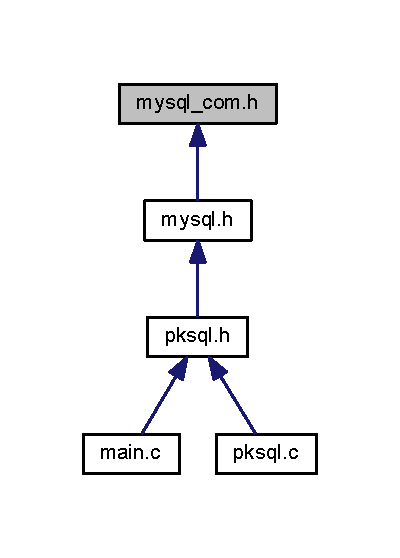
\includegraphics[width=192pt]{mysql__com_8h__dep__incl}
\end{center}
\end{figure}
\subsection*{Data Structures}
\begin{DoxyCompactItemize}
\item 
struct \hyperlink{structst__net}{st\+\_\+net}
\item 
struct \hyperlink{structrand__struct}{rand\+\_\+struct}
\item 
struct \hyperlink{structst__udf__args}{st\+\_\+udf\+\_\+args}
\item 
struct \hyperlink{structst__udf__init}{st\+\_\+udf\+\_\+init}
\end{DoxyCompactItemize}
\subsection*{Macros}
\begin{DoxyCompactItemize}
\item 
\#define \hyperlink{mysql__com_8h_ad9680ec5e05e66d8aef66d444dfd0d6c}{H\+O\+S\+T\+N\+A\+M\+E\+\_\+\+L\+E\+N\+G\+T\+H}~60
\item 
\#define \hyperlink{mysql__com_8h_a5e59beedd9254c2e91bb14abc51b0e66}{S\+Y\+S\+T\+E\+M\+\_\+\+C\+H\+A\+R\+S\+E\+T\+\_\+\+M\+B\+M\+A\+X\+L\+E\+N}~3
\item 
\#define \hyperlink{mysql__com_8h_a891948a8c3b63220ac0428a8982b0810}{N\+A\+M\+E\+\_\+\+C\+H\+A\+R\+\_\+\+L\+E\+N}~64              /$\ast$ Field/table name length $\ast$/
\item 
\#define \hyperlink{mysql__com_8h_aa65480ef272f5363de7cf29995e5d34b}{U\+S\+E\+R\+N\+A\+M\+E\+\_\+\+C\+H\+A\+R\+\_\+\+L\+E\+N\+G\+T\+H}~16
\item 
\#define \hyperlink{mysql__com_8h_a4853f6c25c8394fd57c4d99f61d5cd89}{N\+A\+M\+E\+\_\+\+L\+E\+N}~(\hyperlink{mysql__com_8h_a891948a8c3b63220ac0428a8982b0810}{N\+A\+M\+E\+\_\+\+C\+H\+A\+R\+\_\+\+L\+E\+N}$\ast$\hyperlink{mysql__com_8h_a5e59beedd9254c2e91bb14abc51b0e66}{S\+Y\+S\+T\+E\+M\+\_\+\+C\+H\+A\+R\+S\+E\+T\+\_\+\+M\+B\+M\+A\+X\+L\+E\+N})
\item 
\#define \hyperlink{mysql__com_8h_a63b42dc81a45f8f72a2cca3994c19d0e}{U\+S\+E\+R\+N\+A\+M\+E\+\_\+\+L\+E\+N\+G\+T\+H}~(\hyperlink{mysql__com_8h_aa65480ef272f5363de7cf29995e5d34b}{U\+S\+E\+R\+N\+A\+M\+E\+\_\+\+C\+H\+A\+R\+\_\+\+L\+E\+N\+G\+T\+H}$\ast$\hyperlink{mysql__com_8h_a5e59beedd9254c2e91bb14abc51b0e66}{S\+Y\+S\+T\+E\+M\+\_\+\+C\+H\+A\+R\+S\+E\+T\+\_\+\+M\+B\+M\+A\+X\+L\+E\+N})
\item 
\#define \hyperlink{mysql__com_8h_af90027415d21c1a1bcc4e8ecd52ded0a}{M\+Y\+S\+Q\+L\+\_\+\+A\+U\+T\+O\+D\+E\+T\+E\+C\+T\+\_\+\+C\+H\+A\+R\+S\+E\+T\+\_\+\+N\+A\+M\+E}~\char`\"{}auto\char`\"{}
\item 
\#define \hyperlink{mysql__com_8h_ab0b9b859d6ba34b87c2abc8c14c37236}{S\+E\+R\+V\+E\+R\+\_\+\+V\+E\+R\+S\+I\+O\+N\+\_\+\+L\+E\+N\+G\+T\+H}~60
\item 
\#define \hyperlink{mysql__com_8h_a8e152edf1a0bae8aec7f5d59cebfbea9}{S\+Q\+L\+S\+T\+A\+T\+E\+\_\+\+L\+E\+N\+G\+T\+H}~5
\item 
\#define \hyperlink{mysql__com_8h_ac1ebe5b17a74bb66e984eeb25f34ad0f}{T\+A\+B\+L\+E\+\_\+\+C\+O\+M\+M\+E\+N\+T\+\_\+\+I\+N\+L\+I\+N\+E\+\_\+\+M\+A\+X\+L\+E\+N}~180 /$\ast$ pre 6.\+0\+: 60 characters $\ast$/
\item 
\#define \hyperlink{mysql__com_8h_ae12c1f112618312d73d03c990d446700}{T\+A\+B\+L\+E\+\_\+\+C\+O\+M\+M\+E\+N\+T\+\_\+\+M\+A\+X\+L\+E\+N}~2048
\item 
\#define \hyperlink{mysql__com_8h_a7cb7dadb604a393b9ab933c879470a66}{C\+O\+L\+U\+M\+N\+\_\+\+C\+O\+M\+M\+E\+N\+T\+\_\+\+M\+A\+X\+L\+E\+N}~1024
\item 
\#define \hyperlink{mysql__com_8h_af023e7812656e3893059541ce331ff74}{I\+N\+D\+E\+X\+\_\+\+C\+O\+M\+M\+E\+N\+T\+\_\+\+M\+A\+X\+L\+E\+N}~1024
\item 
\#define \hyperlink{mysql__com_8h_ad3fab42410d77d3cbea1fa9879edab85}{T\+A\+B\+L\+E\+\_\+\+P\+A\+R\+T\+I\+T\+I\+O\+N\+\_\+\+C\+O\+M\+M\+E\+N\+T\+\_\+\+M\+A\+X\+L\+E\+N}~1024
\item 
\#define \hyperlink{mysql__com_8h_a973c680573b37fc359fc68d0707da355}{M\+A\+X\+\_\+\+P\+A\+C\+K\+E\+T\+\_\+\+L\+E\+N\+G\+T\+H}~(256\+L$\ast$256\+L$\ast$256\+L-\/1)
\item 
\#define \hyperlink{mysql__com_8h_a96fa6daf52df2cc70a987dcb2641286c}{U\+S\+E\+R\+\_\+\+H\+O\+S\+T\+\_\+\+B\+U\+F\+F\+\_\+\+S\+I\+Z\+E}~\hyperlink{mysql__com_8h_ad9680ec5e05e66d8aef66d444dfd0d6c}{H\+O\+S\+T\+N\+A\+M\+E\+\_\+\+L\+E\+N\+G\+T\+H} + \hyperlink{mysql__com_8h_a63b42dc81a45f8f72a2cca3994c19d0e}{U\+S\+E\+R\+N\+A\+M\+E\+\_\+\+L\+E\+N\+G\+T\+H} + 2
\item 
\#define \hyperlink{mysql__com_8h_aacebc74ef9a786231060d3a8d8b56d24}{L\+O\+C\+A\+L\+\_\+\+H\+O\+S\+T}~\char`\"{}localhost\char`\"{}
\item 
\#define \hyperlink{mysql__com_8h_a2e7ec16bc8384bd465b76d1bef082ea7}{L\+O\+C\+A\+L\+\_\+\+H\+O\+S\+T\+\_\+\+N\+A\+M\+E\+D\+P\+I\+P\+E}~\char`\"{}.\char`\"{}
\item 
\#define \hyperlink{mysql__com_8h_a45f11cf97b6dec62756b92cbb96f7418}{S\+C\+R\+A\+M\+B\+L\+E\+\_\+\+L\+E\+N\+G\+T\+H}~20
\item 
\#define \hyperlink{mysql__com_8h_ab30febd381c3a66a6f062821e606808b}{A\+U\+T\+H\+\_\+\+P\+L\+U\+G\+I\+N\+\_\+\+D\+A\+T\+A\+\_\+\+P\+A\+R\+T\+\_\+1\+\_\+\+L\+E\+N\+G\+T\+H}~8
\item 
\#define \hyperlink{mysql__com_8h_ac363c5b133ceee9f563f6117c3717963}{S\+C\+R\+A\+M\+B\+L\+E\+D\+\_\+\+P\+A\+S\+S\+W\+O\+R\+D\+\_\+\+C\+H\+A\+R\+\_\+\+L\+E\+N\+G\+T\+H}~(\hyperlink{mysql__com_8h_a45f11cf97b6dec62756b92cbb96f7418}{S\+C\+R\+A\+M\+B\+L\+E\+\_\+\+L\+E\+N\+G\+T\+H}$\ast$2+1)
\item 
\#define \hyperlink{mysql__com_8h_a50377f5ca5b3e92f3931a81fe7b44043}{N\+O\+T\+\_\+\+N\+U\+L\+L\+\_\+\+F\+L\+A\+G}~1		/$\ast$ Field can\textquotesingle{}t be N\+U\+L\+L $\ast$/
\item 
\#define \hyperlink{mysql__com_8h_a06d741340319e92c3ee7139079488ca8}{P\+R\+I\+\_\+\+K\+E\+Y\+\_\+\+F\+L\+A\+G}~2		/$\ast$ Field is part of a primary key $\ast$/
\item 
\#define \hyperlink{mysql__com_8h_a06304a8d611b152cae7b9146741f9cab}{U\+N\+I\+Q\+U\+E\+\_\+\+K\+E\+Y\+\_\+\+F\+L\+A\+G}~4		/$\ast$ Field is part of a unique key $\ast$/
\item 
\#define \hyperlink{mysql__com_8h_a54b877f8dd75234bf29213636f19f70f}{M\+U\+L\+T\+I\+P\+L\+E\+\_\+\+K\+E\+Y\+\_\+\+F\+L\+A\+G}~8		/$\ast$ Field is part of a key $\ast$/
\item 
\#define \hyperlink{mysql__com_8h_a5a1ebc825faa2b47812f514190cefb02}{B\+L\+O\+B\+\_\+\+F\+L\+A\+G}~16		/$\ast$ Field is a blob $\ast$/
\item 
\#define \hyperlink{mysql__com_8h_a141ca01d9275360db8b4502e6d3c2ff2}{U\+N\+S\+I\+G\+N\+E\+D\+\_\+\+F\+L\+A\+G}~32		/$\ast$ Field is unsigned $\ast$/
\item 
\#define \hyperlink{mysql__com_8h_a0e5559ab79365f739055868042f5a081}{Z\+E\+R\+O\+F\+I\+L\+L\+\_\+\+F\+L\+A\+G}~64		/$\ast$ Field is zerofill $\ast$/
\item 
\#define \hyperlink{mysql__com_8h_af74577f0e38eed5616a090965aeac323}{B\+I\+N\+A\+R\+Y\+\_\+\+F\+L\+A\+G}~128		/$\ast$ Field is binary   $\ast$/
\item 
\#define \hyperlink{mysql__com_8h_a0b89f761611b41b80de1f7d50f9b6020}{E\+N\+U\+M\+\_\+\+F\+L\+A\+G}~256		/$\ast$ field is an enum $\ast$/
\item 
\#define \hyperlink{mysql__com_8h_a3ebd2a8abc593a55120f133dd6104c5d}{A\+U\+T\+O\+\_\+\+I\+N\+C\+R\+E\+M\+E\+N\+T\+\_\+\+F\+L\+A\+G}~512		/$\ast$ field is a autoincrement field $\ast$/
\item 
\#define \hyperlink{mysql__com_8h_a2a0ac41ce6f090a6d49739cc2c5c1c25}{T\+I\+M\+E\+S\+T\+A\+M\+P\+\_\+\+F\+L\+A\+G}~1024		/$\ast$ Field is a timestamp $\ast$/
\item 
\#define \hyperlink{mysql__com_8h_a7abab620880927f796581747ae3719c0}{S\+E\+T\+\_\+\+F\+L\+A\+G}~2048		/$\ast$ field is a set $\ast$/
\item 
\#define \hyperlink{mysql__com_8h_a36e0f2111c7f4ead77a90666e345bfd2}{N\+O\+\_\+\+D\+E\+F\+A\+U\+L\+T\+\_\+\+V\+A\+L\+U\+E\+\_\+\+F\+L\+A\+G}~4096	/$\ast$ Field doesn\textquotesingle{}t have default value $\ast$/
\item 
\#define \hyperlink{mysql__com_8h_a9c58a417db90a114db37e0d36f661418}{O\+N\+\_\+\+U\+P\+D\+A\+T\+E\+\_\+\+N\+O\+W\+\_\+\+F\+L\+A\+G}~8192         /$\ast$ Field is set to N\+O\+W on U\+P\+D\+A\+T\+E $\ast$/
\item 
\#define \hyperlink{mysql__com_8h_a76cd81964ebba4dd1dc0a354ad5f279a}{N\+U\+M\+\_\+\+F\+L\+A\+G}~32768		/$\ast$ Field is num (for clients) $\ast$/
\item 
\#define \hyperlink{mysql__com_8h_a6ef113faa3f365ff3a3d0d58eb7fc7aa}{P\+A\+R\+T\+\_\+\+K\+E\+Y\+\_\+\+F\+L\+A\+G}~16384		/$\ast$ Intern; Part of some key $\ast$/
\item 
\#define \hyperlink{mysql__com_8h_a914c4d894f57a4ac193c4cfefc31b2a8}{G\+R\+O\+U\+P\+\_\+\+F\+L\+A\+G}~32768		/$\ast$ Intern\+: Group field $\ast$/
\item 
\#define \hyperlink{mysql__com_8h_a33a9e3d3e386450dee2571dfb412b347}{U\+N\+I\+Q\+U\+E\+\_\+\+F\+L\+A\+G}~65536		/$\ast$ Intern\+: Used by sql\+\_\+yacc $\ast$/
\item 
\#define \hyperlink{mysql__com_8h_ab0f2e6ec879eb0fc2424df6bc991e89b}{B\+I\+N\+C\+M\+P\+\_\+\+F\+L\+A\+G}~131072		/$\ast$ Intern\+: Used by sql\+\_\+yacc $\ast$/
\item 
\#define \hyperlink{mysql__com_8h_acf4300c88984ccd0d49310e5363d7beb}{G\+E\+T\+\_\+\+F\+I\+X\+E\+D\+\_\+\+F\+I\+E\+L\+D\+S\+\_\+\+F\+L\+A\+G}~(1 $<$$<$ 18) /$\ast$ Used to get fields in item tree $\ast$/
\item 
\#define \hyperlink{mysql__com_8h_a245e102a68235c1a012f2b372254a383}{F\+I\+E\+L\+D\+\_\+\+I\+N\+\_\+\+P\+A\+R\+T\+\_\+\+F\+U\+N\+C\+\_\+\+F\+L\+A\+G}~(1 $<$$<$ 19)/$\ast$ Field part of partition func $\ast$/
\item 
\#define \hyperlink{mysql__com_8h_a306e2d0a93c4d537c502cb2eecce4f38}{F\+I\+E\+L\+D\+\_\+\+I\+N\+\_\+\+A\+D\+D\+\_\+\+I\+N\+D\+E\+X}~(1 $<$$<$ 20)
\item 
\#define \hyperlink{mysql__com_8h_aa74461c914174b504e16a37694a6291a}{F\+I\+E\+L\+D\+\_\+\+I\+S\+\_\+\+R\+E\+N\+A\+M\+E\+D}~(1$<$$<$ 21)       /$\ast$ Intern\+: Field is being renamed $\ast$/
\item 
\#define \hyperlink{mysql__com_8h_afc8a49c215f29c3a40d35012042c06cb}{F\+I\+E\+L\+D\+\_\+\+F\+L\+A\+G\+S\+\_\+\+S\+T\+O\+R\+A\+G\+E\+\_\+\+M\+E\+D\+I\+A}~22    /$\ast$ Field storage media, bit 22-\/23 $\ast$/
\item 
\#define \hyperlink{mysql__com_8h_ae1a0212370795712cc92830ffbd9444f}{F\+I\+E\+L\+D\+\_\+\+F\+L\+A\+G\+S\+\_\+\+S\+T\+O\+R\+A\+G\+E\+\_\+\+M\+E\+D\+I\+A\+\_\+\+M\+A\+S\+K}~(3 $<$$<$ \hyperlink{mysql__com_8h_afc8a49c215f29c3a40d35012042c06cb}{F\+I\+E\+L\+D\+\_\+\+F\+L\+A\+G\+S\+\_\+\+S\+T\+O\+R\+A\+G\+E\+\_\+\+M\+E\+D\+I\+A})
\item 
\#define \hyperlink{mysql__com_8h_a0ba0387ece21b863536e63f5d8c1ff42}{F\+I\+E\+L\+D\+\_\+\+F\+L\+A\+G\+S\+\_\+\+C\+O\+L\+U\+M\+N\+\_\+\+F\+O\+R\+M\+A\+T}~24    /$\ast$ Field column format, bit 24-\/25 $\ast$/
\item 
\#define \hyperlink{mysql__com_8h_a4a94ef23abb3d309d9f89d608ac7f2eb}{F\+I\+E\+L\+D\+\_\+\+F\+L\+A\+G\+S\+\_\+\+C\+O\+L\+U\+M\+N\+\_\+\+F\+O\+R\+M\+A\+T\+\_\+\+M\+A\+S\+K}~(3 $<$$<$ \hyperlink{mysql__com_8h_a0ba0387ece21b863536e63f5d8c1ff42}{F\+I\+E\+L\+D\+\_\+\+F\+L\+A\+G\+S\+\_\+\+C\+O\+L\+U\+M\+N\+\_\+\+F\+O\+R\+M\+A\+T})
\item 
\#define \hyperlink{mysql__com_8h_a1e5046b398142ac69c9bd538121d194e}{F\+I\+E\+L\+D\+\_\+\+I\+S\+\_\+\+D\+R\+O\+P\+P\+E\+D}~(1$<$$<$ 26)       /$\ast$ Intern\+: Field is being dropped $\ast$/
\item 
\#define \hyperlink{mysql__com_8h_ad75606b04464c9144051cb498e655eba}{E\+X\+P\+L\+I\+C\+I\+T\+\_\+\+N\+U\+L\+L\+\_\+\+F\+L\+A\+G}
\item 
\#define \hyperlink{mysql__com_8h_abd0b4e170cad1ea4cc971f38e669ee7d}{R\+E\+F\+R\+E\+S\+H\+\_\+\+G\+R\+A\+N\+T}~1	/$\ast$ Refresh grant tables $\ast$/
\item 
\#define \hyperlink{mysql__com_8h_a52ad3d18f4abc5503d6c24d38d26d1d1}{R\+E\+F\+R\+E\+S\+H\+\_\+\+L\+O\+G}~2	/$\ast$ Start on new log file $\ast$/
\item 
\#define \hyperlink{mysql__com_8h_ab2b63e3110ce7348a3de27584303deb4}{R\+E\+F\+R\+E\+S\+H\+\_\+\+T\+A\+B\+L\+E\+S}~4	/$\ast$ close all tables $\ast$/
\item 
\#define \hyperlink{mysql__com_8h_a25485561aef48121115352fc2b1d4b7e}{R\+E\+F\+R\+E\+S\+H\+\_\+\+H\+O\+S\+T\+S}~8	/$\ast$ Flush host cache $\ast$/
\item 
\#define \hyperlink{mysql__com_8h_a00b2c683f25deac0e22380cdb4af8ade}{R\+E\+F\+R\+E\+S\+H\+\_\+\+S\+T\+A\+T\+U\+S}~16	/$\ast$ Flush status variables $\ast$/
\item 
\#define \hyperlink{mysql__com_8h_a1c8c3f8ec3397a53b7965427b0cd0231}{R\+E\+F\+R\+E\+S\+H\+\_\+\+T\+H\+R\+E\+A\+D\+S}~32	/$\ast$ Flush thread cache $\ast$/
\item 
\#define \hyperlink{mysql__com_8h_a40ec2519bd9d5fccbf289dd358c5d1fe}{R\+E\+F\+R\+E\+S\+H\+\_\+\+S\+L\+A\+V\+E}
\item 
\#define \hyperlink{mysql__com_8h_a45f37479a7d8f01ed1cc9fa3ed41fd3f}{R\+E\+F\+R\+E\+S\+H\+\_\+\+M\+A\+S\+T\+E\+R}
\item 
\#define \hyperlink{mysql__com_8h_a65a4c3ee93e38a4d413873a5db91a880}{R\+E\+F\+R\+E\+S\+H\+\_\+\+E\+R\+R\+O\+R\+\_\+\+L\+O\+G}~256 /$\ast$ Rotate only the erorr log $\ast$/
\item 
\#define \hyperlink{mysql__com_8h_a9da820da51f5b96fc5e95749be2d9ccc}{R\+E\+F\+R\+E\+S\+H\+\_\+\+E\+N\+G\+I\+N\+E\+\_\+\+L\+O\+G}~512 /$\ast$ Flush all storage engine logs $\ast$/
\item 
\#define \hyperlink{mysql__com_8h_a285330e0b9fbb5df627a2bb386fddce2}{R\+E\+F\+R\+E\+S\+H\+\_\+\+B\+I\+N\+A\+R\+Y\+\_\+\+L\+O\+G}~1024 /$\ast$ Flush the binary log $\ast$/
\item 
\#define \hyperlink{mysql__com_8h_a0538e6900be81e7039e0439ec5570672}{R\+E\+F\+R\+E\+S\+H\+\_\+\+R\+E\+L\+A\+Y\+\_\+\+L\+O\+G}~2048 /$\ast$ Flush the relay log $\ast$/
\item 
\#define \hyperlink{mysql__com_8h_a8868ef78edd7dc5f5641d64e6aac5cd3}{R\+E\+F\+R\+E\+S\+H\+\_\+\+G\+E\+N\+E\+R\+A\+L\+\_\+\+L\+O\+G}~4096 /$\ast$ Flush the general log $\ast$/
\item 
\#define \hyperlink{mysql__com_8h_a910e4dfce22003b8cb5db1e9364369b2}{R\+E\+F\+R\+E\+S\+H\+\_\+\+S\+L\+O\+W\+\_\+\+L\+O\+G}~8192 /$\ast$ Flush the slow query log $\ast$/
\item 
\#define \hyperlink{mysql__com_8h_a5646ca6d144531040c0c0fdf0e4f08d5}{R\+E\+F\+R\+E\+S\+H\+\_\+\+R\+E\+A\+D\+\_\+\+L\+O\+C\+K}~16384	/$\ast$ Lock tables for read $\ast$/
\item 
\#define \hyperlink{mysql__com_8h_a9dc4f3371c4dd202b46ba39f27d9bf05}{R\+E\+F\+R\+E\+S\+H\+\_\+\+F\+A\+S\+T}~32768	/$\ast$ Intern flag $\ast$/
\item 
\#define \hyperlink{mysql__com_8h_a1d27f6453c74f29279188265535e4d7e}{R\+E\+F\+R\+E\+S\+H\+\_\+\+Q\+U\+E\+R\+Y\+\_\+\+C\+A\+C\+H\+E}~65536
\item 
\#define \hyperlink{mysql__com_8h_a332fb66a7459f1dc7234ed870223e9ec}{R\+E\+F\+R\+E\+S\+H\+\_\+\+Q\+U\+E\+R\+Y\+\_\+\+C\+A\+C\+H\+E\+\_\+\+F\+R\+E\+E}~0x20000\+L /$\ast$ pack query cache $\ast$/
\item 
\#define \hyperlink{mysql__com_8h_a71494bfead804cf67bc7423880836804}{R\+E\+F\+R\+E\+S\+H\+\_\+\+D\+E\+S\+\_\+\+K\+E\+Y\+\_\+\+F\+I\+L\+E}~0x40000\+L
\item 
\#define \hyperlink{mysql__com_8h_a02b07f776c32610833786f108b50d974}{R\+E\+F\+R\+E\+S\+H\+\_\+\+U\+S\+E\+R\+\_\+\+R\+E\+S\+O\+U\+R\+C\+E\+S}~0x80000\+L
\item 
\#define \hyperlink{mysql__com_8h_ada5ac4861632f7a9f1423eac5d8cdccc}{R\+E\+F\+R\+E\+S\+H\+\_\+\+F\+O\+R\+\_\+\+E\+X\+P\+O\+R\+T}~0x100000\+L /$\ast$ F\+L\+U\+S\+H T\+A\+B\+L\+E\+S ... F\+O\+R E\+X\+P\+O\+R\+T $\ast$/
\item 
\#define \hyperlink{mysql__com_8h_acf53446a84fc10d56b57cf5701ec94f9}{R\+E\+F\+R\+E\+S\+H\+\_\+\+O\+P\+T\+I\+M\+I\+Z\+E\+R\+\_\+\+C\+O\+S\+T\+S}~0x200000\+L /$\ast$ F\+L\+U\+S\+H O\+P\+T\+I\+M\+I\+Z\+E\+R\+\_\+\+C\+O\+S\+T\+S $\ast$/
\item 
\#define \hyperlink{mysql__com_8h_a52d3a3f2f6a84a0f427c16bd7bd3df1f}{C\+L\+I\+E\+N\+T\+\_\+\+L\+O\+N\+G\+\_\+\+P\+A\+S\+S\+W\+O\+R\+D}~1	/$\ast$ new more secure passwords $\ast$/
\item 
\#define \hyperlink{mysql__com_8h_a4d108689643f2dfdb9d7fee3e20341af}{C\+L\+I\+E\+N\+T\+\_\+\+F\+O\+U\+N\+D\+\_\+\+R\+O\+W\+S}~2	/$\ast$ Found instead of affected rows $\ast$/
\item 
\#define \hyperlink{mysql__com_8h_acb925b1d791ae381a1b411e26c72db35}{C\+L\+I\+E\+N\+T\+\_\+\+L\+O\+N\+G\+\_\+\+F\+L\+A\+G}~4	/$\ast$ Get all column flags $\ast$/
\item 
\#define \hyperlink{mysql__com_8h_a5077ddf4e9da252588645484d8e2f72f}{C\+L\+I\+E\+N\+T\+\_\+\+C\+O\+N\+N\+E\+C\+T\+\_\+\+W\+I\+T\+H\+\_\+\+D\+B}~8	/$\ast$ One can specify db on connect $\ast$/
\item 
\#define \hyperlink{mysql__com_8h_a55c846cdcebd257a7d065c403a495767}{C\+L\+I\+E\+N\+T\+\_\+\+N\+O\+\_\+\+S\+C\+H\+E\+M\+A}~16	/$\ast$ Don\textquotesingle{}t allow database.\+table.\+column $\ast$/
\item 
\#define \hyperlink{mysql__com_8h_a69668fa642cd688ab5a3c24de87c0b9a}{C\+L\+I\+E\+N\+T\+\_\+\+C\+O\+M\+P\+R\+E\+S\+S}~32	/$\ast$ Can use compression protocol $\ast$/
\item 
\#define \hyperlink{mysql__com_8h_a790a993d52ae9454e8a3fbdfa2fc57fe}{C\+L\+I\+E\+N\+T\+\_\+\+O\+D\+B\+C}~64	/$\ast$ Odbc client $\ast$/
\item 
\#define \hyperlink{mysql__com_8h_a06acc4847890b7ef14a8e7c0782a679c}{C\+L\+I\+E\+N\+T\+\_\+\+L\+O\+C\+A\+L\+\_\+\+F\+I\+L\+E\+S}~128	/$\ast$ Can use L\+O\+A\+D D\+A\+T\+A L\+O\+C\+A\+L $\ast$/
\item 
\#define \hyperlink{mysql__com_8h_a67c9d84d14a0858ccf9c6393c28fb6fb}{C\+L\+I\+E\+N\+T\+\_\+\+I\+G\+N\+O\+R\+E\+\_\+\+S\+P\+A\+C\+E}~256	/$\ast$ Ignore spaces before \textquotesingle{}(\textquotesingle{} $\ast$/
\item 
\#define \hyperlink{mysql__com_8h_acde6ac915ca4c7bc88ae19d7dd9a04c4}{C\+L\+I\+E\+N\+T\+\_\+\+P\+R\+O\+T\+O\+C\+O\+L\+\_\+41}~512	/$\ast$ New 4.\+1 protocol $\ast$/
\item 
\#define \hyperlink{mysql__com_8h_afffcba61df9880b6d17b694f1aaf912f}{C\+L\+I\+E\+N\+T\+\_\+\+I\+N\+T\+E\+R\+A\+C\+T\+I\+V\+E}~1024	/$\ast$ This is an interactive client $\ast$/
\item 
\#define \hyperlink{mysql__com_8h_aa7b23d0f15fbcd6f975df1d6204ea5a2}{C\+L\+I\+E\+N\+T\+\_\+\+S\+S\+L}~2048	/$\ast$ Switch to S\+S\+L after handshake $\ast$/
\item 
\#define \hyperlink{mysql__com_8h_a80b7ec30f78263f55be422853b989a28}{C\+L\+I\+E\+N\+T\+\_\+\+I\+G\+N\+O\+R\+E\+\_\+\+S\+I\+G\+P\+I\+P\+E}~4096    /$\ast$ I\+G\+N\+O\+R\+E sigpipes $\ast$/
\item 
\#define \hyperlink{mysql__com_8h_a536a91524dc8d56bcac63aadc8811f1d}{C\+L\+I\+E\+N\+T\+\_\+\+T\+R\+A\+N\+S\+A\+C\+T\+I\+O\+N\+S}~8192	/$\ast$ Client knows about transactions $\ast$/
\item 
\#define \hyperlink{mysql__com_8h_ad369dc5c503fc75213f86bc3ab6dd466}{C\+L\+I\+E\+N\+T\+\_\+\+R\+E\+S\+E\+R\+V\+E\+D}~16384   /$\ast$ Old flag for 4.\+1 protocol  $\ast$/
\item 
\#define \hyperlink{mysql__com_8h_a8be684cc38eeca913698414efec06933}{C\+L\+I\+E\+N\+T\+\_\+\+R\+E\+S\+E\+R\+V\+E\+D2}~32768   /$\ast$ Old flag for 4.\+1 authentication $\ast$/
\item 
\#define \hyperlink{mysql__com_8h_a5aa1db4db950d645235a4f73263ee911}{C\+L\+I\+E\+N\+T\+\_\+\+M\+U\+L\+T\+I\+\_\+\+S\+T\+A\+T\+E\+M\+E\+N\+T\+S}~(1\+U\+L $<$$<$ 16) /$\ast$ Enable/disable multi-\/stmt support $\ast$/
\item 
\#define \hyperlink{mysql__com_8h_a2ffea3e8918e7c9a3a2323030a2bfe0a}{C\+L\+I\+E\+N\+T\+\_\+\+M\+U\+L\+T\+I\+\_\+\+R\+E\+S\+U\+L\+T\+S}~(1\+U\+L $<$$<$ 17) /$\ast$ Enable/disable multi-\/results $\ast$/
\item 
\#define \hyperlink{mysql__com_8h_a70fe479c539d7e2970fea9a374593ea5}{C\+L\+I\+E\+N\+T\+\_\+\+P\+S\+\_\+\+M\+U\+L\+T\+I\+\_\+\+R\+E\+S\+U\+L\+T\+S}~(1\+U\+L $<$$<$ 18) /$\ast$ Multi-\/results in P\+S-\/protocol $\ast$/
\item 
\#define \hyperlink{mysql__com_8h_a2a6cb83350f95a382a35de3021904012}{C\+L\+I\+E\+N\+T\+\_\+\+P\+L\+U\+G\+I\+N\+\_\+\+A\+U\+T\+H}~(1\+U\+L $<$$<$ 19) /$\ast$ Client supports plugin authentication $\ast$/
\item 
\#define \hyperlink{mysql__com_8h_a57c0b9235a4e8038736a776ab484b862}{C\+L\+I\+E\+N\+T\+\_\+\+C\+O\+N\+N\+E\+C\+T\+\_\+\+A\+T\+T\+R\+S}~(1\+U\+L $<$$<$ 20) /$\ast$ Client supports connection attributes $\ast$/
\item 
\#define \hyperlink{mysql__com_8h_ac2afd7c695ae50763b5c1b7320e812d3}{C\+L\+I\+E\+N\+T\+\_\+\+P\+L\+U\+G\+I\+N\+\_\+\+A\+U\+T\+H\+\_\+\+L\+E\+N\+E\+N\+C\+\_\+\+C\+L\+I\+E\+N\+T\+\_\+\+D\+A\+T\+A}~(1\+U\+L $<$$<$ 21)
\item 
\#define \hyperlink{mysql__com_8h_aab5d2f8647cb4e8e7942d5db98af9efd}{C\+L\+I\+E\+N\+T\+\_\+\+C\+A\+N\+\_\+\+H\+A\+N\+D\+L\+E\+\_\+\+E\+X\+P\+I\+R\+E\+D\+\_\+\+P\+A\+S\+S\+W\+O\+R\+D\+S}~(1\+U\+L $<$$<$ 22)
\item 
\#define \hyperlink{mysql__com_8h_af33ba943944ca32827a1bce983914302}{C\+L\+I\+E\+N\+T\+\_\+\+S\+E\+S\+S\+I\+O\+N\+\_\+\+T\+R\+A\+C\+K}~(1\+U\+L $<$$<$ 23)
\item 
\#define \hyperlink{mysql__com_8h_aad8e6e886899e90e820d6c2e0248469d}{C\+L\+I\+E\+N\+T\+\_\+\+D\+E\+P\+R\+E\+C\+A\+T\+E\+\_\+\+E\+O\+F}~(1\+U\+L $<$$<$ 24)
\item 
\#define \hyperlink{mysql__com_8h_a4e7c0220984fdf1e231344f450cfd51e}{C\+L\+I\+E\+N\+T\+\_\+\+S\+S\+L\+\_\+\+V\+E\+R\+I\+F\+Y\+\_\+\+S\+E\+R\+V\+E\+R\+\_\+\+C\+E\+R\+T}~(1\+U\+L $<$$<$ 30)
\item 
\#define \hyperlink{mysql__com_8h_a07344a4eb8f5c74ea8875bb4e9852fb0}{C\+L\+I\+E\+N\+T\+\_\+\+R\+E\+M\+E\+M\+B\+E\+R\+\_\+\+O\+P\+T\+I\+O\+N\+S}~(1\+U\+L $<$$<$ 31)
\item 
\#define \hyperlink{mysql__com_8h_a8520c7304fb23932e73f951f93217759}{C\+A\+N\+\_\+\+C\+L\+I\+E\+N\+T\+\_\+\+C\+O\+M\+P\+R\+E\+S\+S}~0
\item 
\#define \hyperlink{mysql__com_8h_aa6d2184e6f8c44ef31fc6eec43d60fe5}{C\+L\+I\+E\+N\+T\+\_\+\+A\+L\+L\+\_\+\+F\+L\+A\+G\+S}
\item 
\#define \hyperlink{mysql__com_8h_a3fc90410d0838e40e3ebb8aa047fe445}{C\+L\+I\+E\+N\+T\+\_\+\+B\+A\+S\+I\+C\+\_\+\+F\+L\+A\+G\+S}
\item 
\#define \hyperlink{mysql__com_8h_a8e4ffa42cecc3c43f30c4e1166c37bf9}{S\+E\+R\+V\+E\+R\+\_\+\+S\+T\+A\+T\+U\+S\+\_\+\+I\+N\+\_\+\+T\+R\+A\+N\+S}~1
\item 
\#define \hyperlink{mysql__com_8h_a14de32242085d5ccc469dac547c976b4}{S\+E\+R\+V\+E\+R\+\_\+\+S\+T\+A\+T\+U\+S\+\_\+\+A\+U\+T\+O\+C\+O\+M\+M\+I\+T}~2	/$\ast$ Server in auto\+\_\+commit mode $\ast$/
\item 
\#define \hyperlink{mysql__com_8h_ad1c5060b7e9bead6739fa36f4f09acc3}{S\+E\+R\+V\+E\+R\+\_\+\+M\+O\+R\+E\+\_\+\+R\+E\+S\+U\+L\+T\+S\+\_\+\+E\+X\+I\+S\+T\+S}~8    /$\ast$ Multi query -\/ next query exists $\ast$/
\item 
\#define \hyperlink{mysql__com_8h_a36f6dd235523015dca671341ba85d684}{S\+E\+R\+V\+E\+R\+\_\+\+Q\+U\+E\+R\+Y\+\_\+\+N\+O\+\_\+\+G\+O\+O\+D\+\_\+\+I\+N\+D\+E\+X\+\_\+\+U\+S\+E\+D}~16
\item 
\#define \hyperlink{mysql__com_8h_a36a12f16dcda96f2683fdd696ec45ca8}{S\+E\+R\+V\+E\+R\+\_\+\+Q\+U\+E\+R\+Y\+\_\+\+N\+O\+\_\+\+I\+N\+D\+E\+X\+\_\+\+U\+S\+E\+D}~32
\item 
\#define \hyperlink{mysql__com_8h_a13671267e528760eac66c2a9b5193a1a}{S\+E\+R\+V\+E\+R\+\_\+\+S\+T\+A\+T\+U\+S\+\_\+\+C\+U\+R\+S\+O\+R\+\_\+\+E\+X\+I\+S\+T\+S}~64
\item 
\#define \hyperlink{mysql__com_8h_a52f55b67da86865dc63e87b006c84910}{S\+E\+R\+V\+E\+R\+\_\+\+S\+T\+A\+T\+U\+S\+\_\+\+L\+A\+S\+T\+\_\+\+R\+O\+W\+\_\+\+S\+E\+N\+T}~128
\item 
\#define \hyperlink{mysql__com_8h_ac65f3ca1e5bb1eb7425027e41c0fda78}{S\+E\+R\+V\+E\+R\+\_\+\+S\+T\+A\+T\+U\+S\+\_\+\+D\+B\+\_\+\+D\+R\+O\+P\+P\+E\+D}~256 /$\ast$ A database was dropped $\ast$/
\item 
\#define \hyperlink{mysql__com_8h_ae24ddb976475c835c8686270a174c2e6}{S\+E\+R\+V\+E\+R\+\_\+\+S\+T\+A\+T\+U\+S\+\_\+\+N\+O\+\_\+\+B\+A\+C\+K\+S\+L\+A\+S\+H\+\_\+\+E\+S\+C\+A\+P\+E\+S}~512
\item 
\#define \hyperlink{mysql__com_8h_aa288f0eb750f49d17b0f20faac609439}{S\+E\+R\+V\+E\+R\+\_\+\+S\+T\+A\+T\+U\+S\+\_\+\+M\+E\+T\+A\+D\+A\+T\+A\+\_\+\+C\+H\+A\+N\+G\+E\+D}~1024
\item 
\#define \hyperlink{mysql__com_8h_a447fdf106600d80d981bf15cfe77fa90}{S\+E\+R\+V\+E\+R\+\_\+\+Q\+U\+E\+R\+Y\+\_\+\+W\+A\+S\+\_\+\+S\+L\+O\+W}~2048
\item 
\#define \hyperlink{mysql__com_8h_a456838253001479240da8acab13452a9}{S\+E\+R\+V\+E\+R\+\_\+\+P\+S\+\_\+\+O\+U\+T\+\_\+\+P\+A\+R\+A\+M\+S}~4096
\item 
\#define \hyperlink{mysql__com_8h_aee66d782683a7d7029abdb0c06c8f4da}{S\+E\+R\+V\+E\+R\+\_\+\+S\+T\+A\+T\+U\+S\+\_\+\+I\+N\+\_\+\+T\+R\+A\+N\+S\+\_\+\+R\+E\+A\+D\+O\+N\+L\+Y}~8192
\item 
\#define \hyperlink{mysql__com_8h_a639b164580b497128ebe12fcc651de7a}{S\+E\+R\+V\+E\+R\+\_\+\+S\+E\+S\+S\+I\+O\+N\+\_\+\+S\+T\+A\+T\+E\+\_\+\+C\+H\+A\+N\+G\+E\+D}~(1\+U\+L $<$$<$ 14)
\item 
\#define \hyperlink{mysql__com_8h_afdd50a9653e547e25b9a85c35f00b724}{S\+E\+R\+V\+E\+R\+\_\+\+S\+T\+A\+T\+U\+S\+\_\+\+C\+L\+E\+A\+R\+\_\+\+S\+E\+T}
\item 
\#define \hyperlink{mysql__com_8h_a3f5f3eab30894e1dfa8d5bd977a889be}{M\+Y\+S\+Q\+L\+\_\+\+E\+R\+R\+M\+S\+G\+\_\+\+S\+I\+Z\+E}~512
\item 
\#define \hyperlink{mysql__com_8h_a9dc7288e3d1fe554340d18bd27578027}{N\+E\+T\+\_\+\+R\+E\+A\+D\+\_\+\+T\+I\+M\+E\+O\+U\+T}~30		/$\ast$ Timeout on read $\ast$/
\item 
\#define \hyperlink{mysql__com_8h_af62b1879e97bbca88f124748f9af8baf}{N\+E\+T\+\_\+\+W\+R\+I\+T\+E\+\_\+\+T\+I\+M\+E\+O\+U\+T}~60		/$\ast$ Timeout on write $\ast$/
\item 
\#define \hyperlink{mysql__com_8h_a075b3b44b67034e9379f49d0eeacc1d4}{N\+E\+T\+\_\+\+W\+A\+I\+T\+\_\+\+T\+I\+M\+E\+O\+U\+T}~8$\ast$60$\ast$60		/$\ast$ Wait for new query $\ast$/
\item 
\#define \hyperlink{mysql__com_8h_aff681008e30f507179af6585629be2d2}{O\+N\+L\+Y\+\_\+\+K\+I\+L\+L\+\_\+\+Q\+U\+E\+R\+Y}~1
\item 
\#define \hyperlink{mysql__com_8h_a33da5943604e3165054a0dd6662e57cf}{M\+A\+X\+\_\+\+T\+I\+N\+Y\+I\+N\+T\+\_\+\+W\+I\+D\+T\+H}~3       /$\ast$ Max width for a T\+I\+N\+Y w.\+o. sign $\ast$/
\item 
\#define \hyperlink{mysql__com_8h_afb96a5507eb70ae640ae37bf7faa97e7}{M\+A\+X\+\_\+\+S\+M\+A\+L\+L\+I\+N\+T\+\_\+\+W\+I\+D\+T\+H}~5       /$\ast$ Max width for a S\+H\+O\+R\+T w.\+o. sign $\ast$/
\item 
\#define \hyperlink{mysql__com_8h_a670b6b78bc553951352f4a8460cbf640}{M\+A\+X\+\_\+\+M\+E\+D\+I\+U\+M\+I\+N\+T\+\_\+\+W\+I\+D\+T\+H}~8       /$\ast$ Max width for a I\+N\+T24 w.\+o. sign $\ast$/
\item 
\#define \hyperlink{mysql__com_8h_ac3232b5227e5811b50f8d62762263ce0}{M\+A\+X\+\_\+\+I\+N\+T\+\_\+\+W\+I\+D\+T\+H}~10      /$\ast$ Max width for a L\+O\+N\+G w.\+o. sign $\ast$/
\item 
\#define \hyperlink{mysql__com_8h_a884564a4714fe1f4af631a33af60c6bf}{M\+A\+X\+\_\+\+B\+I\+G\+I\+N\+T\+\_\+\+W\+I\+D\+T\+H}~20      /$\ast$ Max width for a L\+O\+N\+G\+L\+O\+N\+G $\ast$/
\item 
\#define \hyperlink{mysql__com_8h_aee01741f0b87b67bcc04c1aec2dc61e2}{M\+A\+X\+\_\+\+C\+H\+A\+R\+\_\+\+W\+I\+D\+T\+H}~255	/$\ast$ Max length for a C\+H\+A\+R colum $\ast$/
\item 
\#define \hyperlink{mysql__com_8h_a32d8ffae76978154421c4c446f221ab3}{M\+A\+X\+\_\+\+B\+L\+O\+B\+\_\+\+W\+I\+D\+T\+H}~16777216	/$\ast$ Default width for blob $\ast$/
\item 
\#define \hyperlink{mysql__com_8h_a08253bf6eaa0178369f3ee1055b914a0}{packet\+\_\+error}~($\sim$(unsigned long) 0)
\item 
\#define \hyperlink{mysql__com_8h_a6a56572c4bd65c8f3e71949fefe8f9bb}{C\+L\+I\+E\+N\+T\+\_\+\+M\+U\+L\+T\+I\+\_\+\+Q\+U\+E\+R\+I\+E\+S}~\hyperlink{mysql__com_8h_a5aa1db4db950d645235a4f73263ee911}{C\+L\+I\+E\+N\+T\+\_\+\+M\+U\+L\+T\+I\+\_\+\+S\+T\+A\+T\+E\+M\+E\+N\+T\+S}
\item 
\#define \hyperlink{mysql__com_8h_a90be5b1946365670d2debb7cd3a8554a}{F\+I\+E\+L\+D\+\_\+\+T\+Y\+P\+E\+\_\+\+D\+E\+C\+I\+M\+A\+L}~\hyperlink{mysql__com_8h_a69e798807026a0f7e12b1d6c72374854ad06d7fa5c7a7110a3586412e7b2f5383}{M\+Y\+S\+Q\+L\+\_\+\+T\+Y\+P\+E\+\_\+\+D\+E\+C\+I\+M\+A\+L}
\item 
\#define \hyperlink{mysql__com_8h_a47e03d9b3a1a4a35ff23b4b681ca76e4}{F\+I\+E\+L\+D\+\_\+\+T\+Y\+P\+E\+\_\+\+N\+E\+W\+D\+E\+C\+I\+M\+A\+L}~\hyperlink{mysql__com_8h_a69e798807026a0f7e12b1d6c72374854abf1e0aa5e259fe4d630043c94f6f693a}{M\+Y\+S\+Q\+L\+\_\+\+T\+Y\+P\+E\+\_\+\+N\+E\+W\+D\+E\+C\+I\+M\+A\+L}
\item 
\#define \hyperlink{mysql__com_8h_acdf494414f6c429abb10ac66d060e146}{F\+I\+E\+L\+D\+\_\+\+T\+Y\+P\+E\+\_\+\+T\+I\+N\+Y}~\hyperlink{mysql__com_8h_a69e798807026a0f7e12b1d6c72374854a33aad6613c99ffbdd65104a310367c0e}{M\+Y\+S\+Q\+L\+\_\+\+T\+Y\+P\+E\+\_\+\+T\+I\+N\+Y}
\item 
\#define \hyperlink{mysql__com_8h_a9a8b52296370dad676e9eac160c1e2c9}{F\+I\+E\+L\+D\+\_\+\+T\+Y\+P\+E\+\_\+\+S\+H\+O\+R\+T}~\hyperlink{mysql__com_8h_a69e798807026a0f7e12b1d6c72374854adf6833ce40915c6b41428330512c2981}{M\+Y\+S\+Q\+L\+\_\+\+T\+Y\+P\+E\+\_\+\+S\+H\+O\+R\+T}
\item 
\#define \hyperlink{mysql__com_8h_a369b93d54934f4b429ea91e1fa8eebc7}{F\+I\+E\+L\+D\+\_\+\+T\+Y\+P\+E\+\_\+\+L\+O\+N\+G}~\hyperlink{mysql__com_8h_a69e798807026a0f7e12b1d6c72374854abc4146fed5436366231421db171b1bda}{M\+Y\+S\+Q\+L\+\_\+\+T\+Y\+P\+E\+\_\+\+L\+O\+N\+G}
\item 
\#define \hyperlink{mysql__com_8h_a8d2be0344cc0f344e49e682a85ceaf3f}{F\+I\+E\+L\+D\+\_\+\+T\+Y\+P\+E\+\_\+\+F\+L\+O\+A\+T}~\hyperlink{mysql__com_8h_a69e798807026a0f7e12b1d6c72374854ae620a5b03bf1c08211cd3b2b9885e802}{M\+Y\+S\+Q\+L\+\_\+\+T\+Y\+P\+E\+\_\+\+F\+L\+O\+A\+T}
\item 
\#define \hyperlink{mysql__com_8h_a4fd682275d6d80f32898a373cfc6a7e9}{F\+I\+E\+L\+D\+\_\+\+T\+Y\+P\+E\+\_\+\+D\+O\+U\+B\+L\+E}~\hyperlink{mysql__com_8h_a69e798807026a0f7e12b1d6c72374854ad4e0c04e294f1f9c060b9fb37646670f}{M\+Y\+S\+Q\+L\+\_\+\+T\+Y\+P\+E\+\_\+\+D\+O\+U\+B\+L\+E}
\item 
\#define \hyperlink{mysql__com_8h_ae92e075709274319f90eb0f3d36a2b6e}{F\+I\+E\+L\+D\+\_\+\+T\+Y\+P\+E\+\_\+\+N\+U\+L\+L}~\hyperlink{mysql__com_8h_a69e798807026a0f7e12b1d6c72374854a7cb889259c4dcce895f048c15f1bb986}{M\+Y\+S\+Q\+L\+\_\+\+T\+Y\+P\+E\+\_\+\+N\+U\+L\+L}
\item 
\#define \hyperlink{mysql__com_8h_a9e9a8f17b8290e653e12e751a39a36a2}{F\+I\+E\+L\+D\+\_\+\+T\+Y\+P\+E\+\_\+\+T\+I\+M\+E\+S\+T\+A\+M\+P}~\hyperlink{mysql__com_8h_a69e798807026a0f7e12b1d6c72374854ae9057027fedb101da18b352d4784fcb0}{M\+Y\+S\+Q\+L\+\_\+\+T\+Y\+P\+E\+\_\+\+T\+I\+M\+E\+S\+T\+A\+M\+P}
\item 
\#define \hyperlink{mysql__com_8h_a3cae40149d16ffedbe110308c726ac77}{F\+I\+E\+L\+D\+\_\+\+T\+Y\+P\+E\+\_\+\+L\+O\+N\+G\+L\+O\+N\+G}~\hyperlink{mysql__com_8h_a69e798807026a0f7e12b1d6c72374854a2324a409d98e39c7868cf04ee538accf}{M\+Y\+S\+Q\+L\+\_\+\+T\+Y\+P\+E\+\_\+\+L\+O\+N\+G\+L\+O\+N\+G}
\item 
\#define \hyperlink{mysql__com_8h_a720a3473d25ab6e0fd09ada85ea099f5}{F\+I\+E\+L\+D\+\_\+\+T\+Y\+P\+E\+\_\+\+I\+N\+T24}~\hyperlink{mysql__com_8h_a69e798807026a0f7e12b1d6c72374854aee0b45950ddbb0f51bdd2ee086552aba}{M\+Y\+S\+Q\+L\+\_\+\+T\+Y\+P\+E\+\_\+\+I\+N\+T24}
\item 
\#define \hyperlink{mysql__com_8h_aa92ca928a7294349c4a4141ab2992e26}{F\+I\+E\+L\+D\+\_\+\+T\+Y\+P\+E\+\_\+\+D\+A\+T\+E}~\hyperlink{mysql__com_8h_a69e798807026a0f7e12b1d6c72374854ae079914b6d07d12feb7cd8f2112c8669}{M\+Y\+S\+Q\+L\+\_\+\+T\+Y\+P\+E\+\_\+\+D\+A\+T\+E}
\item 
\#define \hyperlink{mysql__com_8h_a4b87b016f3984df90f129476f7932a68}{F\+I\+E\+L\+D\+\_\+\+T\+Y\+P\+E\+\_\+\+T\+I\+M\+E}~\hyperlink{mysql__com_8h_a69e798807026a0f7e12b1d6c72374854a54fd5c4e8f77b36b56dea9bac0a3ace5}{M\+Y\+S\+Q\+L\+\_\+\+T\+Y\+P\+E\+\_\+\+T\+I\+M\+E}
\item 
\#define \hyperlink{mysql__com_8h_a77bd5c0fd9d82f30482ad99bf6dccb0d}{F\+I\+E\+L\+D\+\_\+\+T\+Y\+P\+E\+\_\+\+D\+A\+T\+E\+T\+I\+M\+E}~\hyperlink{mysql__com_8h_a69e798807026a0f7e12b1d6c72374854af006d3204bc1d7560d88144db5d11687}{M\+Y\+S\+Q\+L\+\_\+\+T\+Y\+P\+E\+\_\+\+D\+A\+T\+E\+T\+I\+M\+E}
\item 
\#define \hyperlink{mysql__com_8h_ac2f66d7d01588545be65cc82007e891b}{F\+I\+E\+L\+D\+\_\+\+T\+Y\+P\+E\+\_\+\+Y\+E\+A\+R}~\hyperlink{mysql__com_8h_a69e798807026a0f7e12b1d6c72374854af56f96ba1e7d7cf216d987f8dce9650e}{M\+Y\+S\+Q\+L\+\_\+\+T\+Y\+P\+E\+\_\+\+Y\+E\+A\+R}
\item 
\#define \hyperlink{mysql__com_8h_a26713c1b5122794fcb6b24470abc0211}{F\+I\+E\+L\+D\+\_\+\+T\+Y\+P\+E\+\_\+\+N\+E\+W\+D\+A\+T\+E}~\hyperlink{mysql__com_8h_a69e798807026a0f7e12b1d6c72374854a5dd53066c09f8866482760e121979579}{M\+Y\+S\+Q\+L\+\_\+\+T\+Y\+P\+E\+\_\+\+N\+E\+W\+D\+A\+T\+E}
\item 
\#define \hyperlink{mysql__com_8h_a724fed1271c6279b32b3cac2f3883430}{F\+I\+E\+L\+D\+\_\+\+T\+Y\+P\+E\+\_\+\+E\+N\+U\+M}~\hyperlink{mysql__com_8h_a69e798807026a0f7e12b1d6c72374854a95f10bcceced04dae12e1cb2eeef60ac}{M\+Y\+S\+Q\+L\+\_\+\+T\+Y\+P\+E\+\_\+\+E\+N\+U\+M}
\item 
\#define \hyperlink{mysql__com_8h_a5f28b6311f80dc3bf724aca3bc025da1}{F\+I\+E\+L\+D\+\_\+\+T\+Y\+P\+E\+\_\+\+S\+E\+T}~\hyperlink{mysql__com_8h_a69e798807026a0f7e12b1d6c72374854a5591bd9f21855a6f9a25af73acd32864}{M\+Y\+S\+Q\+L\+\_\+\+T\+Y\+P\+E\+\_\+\+S\+E\+T}
\item 
\#define \hyperlink{mysql__com_8h_ab727ec047390e791e0dcb097eee306ee}{F\+I\+E\+L\+D\+\_\+\+T\+Y\+P\+E\+\_\+\+T\+I\+N\+Y\+\_\+\+B\+L\+O\+B}~\hyperlink{mysql__com_8h_a69e798807026a0f7e12b1d6c72374854a9b4a7755878cc06fccbfef853d2f7d1b}{M\+Y\+S\+Q\+L\+\_\+\+T\+Y\+P\+E\+\_\+\+T\+I\+N\+Y\+\_\+\+B\+L\+O\+B}
\item 
\#define \hyperlink{mysql__com_8h_a939379516e9e9689326e84868526eaef}{F\+I\+E\+L\+D\+\_\+\+T\+Y\+P\+E\+\_\+\+M\+E\+D\+I\+U\+M\+\_\+\+B\+L\+O\+B}~\hyperlink{mysql__com_8h_a69e798807026a0f7e12b1d6c72374854adc7436ed1cffe11ff49e10d83a225df1}{M\+Y\+S\+Q\+L\+\_\+\+T\+Y\+P\+E\+\_\+\+M\+E\+D\+I\+U\+M\+\_\+\+B\+L\+O\+B}
\item 
\#define \hyperlink{mysql__com_8h_a1aa1360ca7acd58b4726eee8a75adaf1}{F\+I\+E\+L\+D\+\_\+\+T\+Y\+P\+E\+\_\+\+L\+O\+N\+G\+\_\+\+B\+L\+O\+B}~\hyperlink{mysql__com_8h_a69e798807026a0f7e12b1d6c72374854a23f1862391ccba964e98d14c052af793}{M\+Y\+S\+Q\+L\+\_\+\+T\+Y\+P\+E\+\_\+\+L\+O\+N\+G\+\_\+\+B\+L\+O\+B}
\item 
\#define \hyperlink{mysql__com_8h_a7736a8d79a6e9aa7bb5f7e4bd62179c8}{F\+I\+E\+L\+D\+\_\+\+T\+Y\+P\+E\+\_\+\+B\+L\+O\+B}~\hyperlink{mysql__com_8h_a69e798807026a0f7e12b1d6c72374854a2efdd2d6cc168c5c760f0b9f3416f0f6}{M\+Y\+S\+Q\+L\+\_\+\+T\+Y\+P\+E\+\_\+\+B\+L\+O\+B}
\item 
\#define \hyperlink{mysql__com_8h_aeef0f9492cc4150775f9c1d0a1966481}{F\+I\+E\+L\+D\+\_\+\+T\+Y\+P\+E\+\_\+\+V\+A\+R\+\_\+\+S\+T\+R\+I\+N\+G}~\hyperlink{mysql__com_8h_a69e798807026a0f7e12b1d6c72374854a295cc2f856def410c040f8c5ff00c6c6}{M\+Y\+S\+Q\+L\+\_\+\+T\+Y\+P\+E\+\_\+\+V\+A\+R\+\_\+\+S\+T\+R\+I\+N\+G}
\item 
\#define \hyperlink{mysql__com_8h_ac0e760f4f95eb599358c3e39e59eba81}{F\+I\+E\+L\+D\+\_\+\+T\+Y\+P\+E\+\_\+\+S\+T\+R\+I\+N\+G}~\hyperlink{mysql__com_8h_a69e798807026a0f7e12b1d6c72374854a71bd15e06b1280e3a881af8c50767180}{M\+Y\+S\+Q\+L\+\_\+\+T\+Y\+P\+E\+\_\+\+S\+T\+R\+I\+N\+G}
\item 
\#define \hyperlink{mysql__com_8h_a4d7a75cb2b4d3b5dceb303e553e49a17}{F\+I\+E\+L\+D\+\_\+\+T\+Y\+P\+E\+\_\+\+C\+H\+A\+R}~\hyperlink{mysql__com_8h_a69e798807026a0f7e12b1d6c72374854a33aad6613c99ffbdd65104a310367c0e}{M\+Y\+S\+Q\+L\+\_\+\+T\+Y\+P\+E\+\_\+\+T\+I\+N\+Y}
\item 
\#define \hyperlink{mysql__com_8h_ada8a9ccd848ebcaa05bbf6b327f121c4}{F\+I\+E\+L\+D\+\_\+\+T\+Y\+P\+E\+\_\+\+I\+N\+T\+E\+R\+V\+A\+L}~\hyperlink{mysql__com_8h_a69e798807026a0f7e12b1d6c72374854a95f10bcceced04dae12e1cb2eeef60ac}{M\+Y\+S\+Q\+L\+\_\+\+T\+Y\+P\+E\+\_\+\+E\+N\+U\+M}
\item 
\#define \hyperlink{mysql__com_8h_a83be34da09d80440f7884c1c006ff0f7}{F\+I\+E\+L\+D\+\_\+\+T\+Y\+P\+E\+\_\+\+G\+E\+O\+M\+E\+T\+R\+Y}~\hyperlink{mysql__com_8h_a69e798807026a0f7e12b1d6c72374854abed334e9b472bba8e24e68dde204ec9f}{M\+Y\+S\+Q\+L\+\_\+\+T\+Y\+P\+E\+\_\+\+G\+E\+O\+M\+E\+T\+R\+Y}
\item 
\#define \hyperlink{mysql__com_8h_a0dc70c6317e2162a666ab98409486a67}{F\+I\+E\+L\+D\+\_\+\+T\+Y\+P\+E\+\_\+\+B\+I\+T}~\hyperlink{mysql__com_8h_a69e798807026a0f7e12b1d6c72374854abcb9aa459c8c25906b2855000027485e}{M\+Y\+S\+Q\+L\+\_\+\+T\+Y\+P\+E\+\_\+\+B\+I\+T}
\item 
\#define \hyperlink{mysql__com_8h_a5553201b80b131630b02a2818e059019}{M\+Y\+S\+Q\+L\+\_\+\+S\+H\+U\+T\+D\+O\+W\+N\+\_\+\+K\+I\+L\+L\+A\+B\+L\+E\+\_\+\+C\+O\+N\+N\+E\+C\+T}~(unsigned char)(1 $<$$<$ 0)
\item 
\#define \hyperlink{mysql__com_8h_ac80a404640f68d2e6017842d0609f633}{M\+Y\+S\+Q\+L\+\_\+\+S\+H\+U\+T\+D\+O\+W\+N\+\_\+\+K\+I\+L\+L\+A\+B\+L\+E\+\_\+\+T\+R\+A\+N\+S}~(unsigned char)(1 $<$$<$ 1)
\item 
\#define \hyperlink{mysql__com_8h_a73052c09ce3d73ef5930a44acb7c7e1c}{M\+Y\+S\+Q\+L\+\_\+\+S\+H\+U\+T\+D\+O\+W\+N\+\_\+\+K\+I\+L\+L\+A\+B\+L\+E\+\_\+\+L\+O\+C\+K\+\_\+\+T\+A\+B\+L\+E}~(unsigned char)(1 $<$$<$ 2)
\item 
\#define \hyperlink{mysql__com_8h_ac470831004e3090ca0e9bf6efea0e9a4}{M\+Y\+S\+Q\+L\+\_\+\+S\+H\+U\+T\+D\+O\+W\+N\+\_\+\+K\+I\+L\+L\+A\+B\+L\+E\+\_\+\+U\+P\+D\+A\+T\+E}~(unsigned char)(1 $<$$<$ 3)
\item 
\#define \hyperlink{mysql__com_8h_aa685c756e1bbb1271cb9a07a0132f23c}{S\+E\+S\+S\+I\+O\+N\+\_\+\+T\+R\+A\+C\+K\+\_\+\+B\+E\+G\+I\+N}~\hyperlink{mysql__com_8h_a1c6cf2629b0bda6da6788a25725d6b7faf5db7e3d564b77cb9bff54a4ca698f78}{S\+E\+S\+S\+I\+O\+N\+\_\+\+T\+R\+A\+C\+K\+\_\+\+S\+Y\+S\+T\+E\+M\+\_\+\+V\+A\+R\+I\+A\+B\+L\+E\+S}
\item 
\#define \hyperlink{mysql__com_8h_ae08eede773abceab702749ac56d39fc4}{S\+E\+S\+S\+I\+O\+N\+\_\+\+T\+R\+A\+C\+K\+\_\+\+E\+N\+D}~\hyperlink{mysql__com_8h_a1c6cf2629b0bda6da6788a25725d6b7fab226cb02bce4e87526fcd8aebf071c6e}{S\+E\+S\+S\+I\+O\+N\+\_\+\+T\+R\+A\+C\+K\+\_\+\+S\+T\+A\+T\+E\+\_\+\+C\+H\+A\+N\+G\+E}
\item 
\#define \hyperlink{mysql__com_8h_a3ef27dda96abec1b380d8d164d22aad1}{I\+S\+\_\+\+S\+E\+S\+S\+I\+O\+N\+\_\+\+S\+T\+A\+T\+E\+\_\+\+T\+Y\+P\+E}(T)~(((int)(T) $>$= \hyperlink{mysql__com_8h_aa685c756e1bbb1271cb9a07a0132f23c}{S\+E\+S\+S\+I\+O\+N\+\_\+\+T\+R\+A\+C\+K\+\_\+\+B\+E\+G\+I\+N}) \&\& ((T) $<$= \hyperlink{mysql__com_8h_ae08eede773abceab702749ac56d39fc4}{S\+E\+S\+S\+I\+O\+N\+\_\+\+T\+R\+A\+C\+K\+\_\+\+E\+N\+D}))
\item 
\#define \hyperlink{mysql__com_8h_a0338154cdba19d8f979b04386bfd9154}{net\+\_\+new\+\_\+transaction}(net)~((net)-\/$>$pkt\+\_\+nr=0)
\item 
\#define \hyperlink{mysql__com_8h_ae6564c0f9410928921c747542d2b53f5}{N\+E\+T\+\_\+\+H\+E\+A\+D\+E\+R\+\_\+\+S\+I\+Z\+E}~4		/$\ast$ standard header size $\ast$/
\item 
\#define \hyperlink{mysql__com_8h_a96b9fe0154bb8a7608f8a2708992ab3e}{C\+O\+M\+P\+\_\+\+H\+E\+A\+D\+E\+R\+\_\+\+S\+I\+Z\+E}~3		/$\ast$ compression header extra size $\ast$/
\item 
\#define \hyperlink{mysql__com_8h_a68145c6add783b349707b9889d33de6c}{N\+U\+L\+L\+\_\+\+L\+E\+N\+G\+T\+H}~((unsigned long) $\sim$0) /$\ast$ For net\+\_\+store\+\_\+length $\ast$/
\item 
\#define \hyperlink{mysql__com_8h_a9f0407504247b1ded701911ccba4bac7}{M\+Y\+S\+Q\+L\+\_\+\+S\+T\+M\+T\+\_\+\+H\+E\+A\+D\+E\+R}~4
\item 
\#define \hyperlink{mysql__com_8h_a64db8802e4fad46ad1619fd641112f69}{M\+Y\+S\+Q\+L\+\_\+\+L\+O\+N\+G\+\_\+\+D\+A\+T\+A\+\_\+\+H\+E\+A\+D\+E\+R}~6
\item 
\#define \hyperlink{mysql__com_8h_aba32bd2e8f3d1153035b14ec074b8e81}{N\+O\+T\+\_\+\+F\+I\+X\+E\+D\+\_\+\+D\+E\+C}~31
\end{DoxyCompactItemize}
\subsection*{Typedefs}
\begin{DoxyCompactItemize}
\item 
typedef struct st\+\_\+vio \hyperlink{mysql__com_8h_a398c428bc2e077b9c404e6b81b813c5c}{Vio}
\item 
typedef struct \hyperlink{structst__net}{st\+\_\+net} \hyperlink{mysql__com_8h_a6869c9fe9e26bbedea92d6603825d482}{N\+E\+T}
\item 
typedef struct \hyperlink{structst__udf__args}{st\+\_\+udf\+\_\+args} \hyperlink{mysql__com_8h_a9cd97a19a143b06969e8ca1a55958a43}{U\+D\+F\+\_\+\+A\+R\+G\+S}
\item 
typedef struct \hyperlink{structst__udf__init}{st\+\_\+udf\+\_\+init} \hyperlink{mysql__com_8h_a9936ce95fffc102cd46ffcde3d659f99}{U\+D\+F\+\_\+\+I\+N\+I\+T}
\end{DoxyCompactItemize}
\subsection*{Enumerations}
\begin{DoxyCompactItemize}
\item 
enum \hyperlink{mysql__com_8h_ae2ff1badf13d2b8099af8b47831281e1}{enum\+\_\+server\+\_\+command} \{ \\*
\hyperlink{mysql__com_8h_ae2ff1badf13d2b8099af8b47831281e1ad65b59a705d1ad995b5d4b11e8a0ea89}{C\+O\+M\+\_\+\+S\+L\+E\+E\+P}, 
\hyperlink{mysql__com_8h_ae2ff1badf13d2b8099af8b47831281e1a1bbc2d425b64d5a0f32f17bbf201fbb2}{C\+O\+M\+\_\+\+Q\+U\+I\+T}, 
\hyperlink{mysql__com_8h_ae2ff1badf13d2b8099af8b47831281e1aebf91bc694c68a0d92c3adcc1bf61a2d}{C\+O\+M\+\_\+\+I\+N\+I\+T\+\_\+\+D\+B}, 
\hyperlink{mysql__com_8h_ae2ff1badf13d2b8099af8b47831281e1a753ea4f670b155bf3f6f2bdf85431fc8}{C\+O\+M\+\_\+\+Q\+U\+E\+R\+Y}, 
\\*
\hyperlink{mysql__com_8h_ae2ff1badf13d2b8099af8b47831281e1af606bae27d05797cd52037904d24a18a}{C\+O\+M\+\_\+\+F\+I\+E\+L\+D\+\_\+\+L\+I\+S\+T}, 
\hyperlink{mysql__com_8h_ae2ff1badf13d2b8099af8b47831281e1a9af6bd3ae3311268b8a84d63ee314caf}{C\+O\+M\+\_\+\+C\+R\+E\+A\+T\+E\+\_\+\+D\+B}, 
\hyperlink{mysql__com_8h_ae2ff1badf13d2b8099af8b47831281e1a2b7df2e35f15c4d4b6401ce6cea670d2}{C\+O\+M\+\_\+\+D\+R\+O\+P\+\_\+\+D\+B}, 
\hyperlink{mysql__com_8h_ae2ff1badf13d2b8099af8b47831281e1a8a8086f9c1bffcbc6e82653f4190f2bd}{C\+O\+M\+\_\+\+R\+E\+F\+R\+E\+S\+H}, 
\\*
\hyperlink{mysql__com_8h_ae2ff1badf13d2b8099af8b47831281e1a958b2095498cd24b57b8c7cb2357b5fa}{C\+O\+M\+\_\+\+S\+H\+U\+T\+D\+O\+W\+N}, 
\hyperlink{mysql__com_8h_ae2ff1badf13d2b8099af8b47831281e1a6cd6011dcafe2bcfa37f75299cc85f4d}{C\+O\+M\+\_\+\+S\+T\+A\+T\+I\+S\+T\+I\+C\+S}, 
\hyperlink{mysql__com_8h_ae2ff1badf13d2b8099af8b47831281e1a0ae3fb92fa55105c8a0a29bb9172c1ab}{C\+O\+M\+\_\+\+P\+R\+O\+C\+E\+S\+S\+\_\+\+I\+N\+F\+O}, 
\hyperlink{mysql__com_8h_ae2ff1badf13d2b8099af8b47831281e1a0dc52f55f182e5badb02156bfdab919b}{C\+O\+M\+\_\+\+C\+O\+N\+N\+E\+C\+T}, 
\\*
\hyperlink{mysql__com_8h_ae2ff1badf13d2b8099af8b47831281e1afc0809078321d9b25c4b6d91f7d1dc21}{C\+O\+M\+\_\+\+P\+R\+O\+C\+E\+S\+S\+\_\+\+K\+I\+L\+L}, 
\hyperlink{mysql__com_8h_ae2ff1badf13d2b8099af8b47831281e1a13465520e09b4ef5844e863a993235a3}{C\+O\+M\+\_\+\+D\+E\+B\+U\+G}, 
\hyperlink{mysql__com_8h_ae2ff1badf13d2b8099af8b47831281e1a2ab6f3fe76c3762bf7d3b6e8ba0a6968}{C\+O\+M\+\_\+\+P\+I\+N\+G}, 
\hyperlink{mysql__com_8h_ae2ff1badf13d2b8099af8b47831281e1aab947848a179d5656091ac5167db3204}{C\+O\+M\+\_\+\+T\+I\+M\+E}, 
\\*
\hyperlink{mysql__com_8h_ae2ff1badf13d2b8099af8b47831281e1a6335cc1ea4cafe148692ffc3613ebb26}{C\+O\+M\+\_\+\+D\+E\+L\+A\+Y\+E\+D\+\_\+\+I\+N\+S\+E\+R\+T}, 
\hyperlink{mysql__com_8h_ae2ff1badf13d2b8099af8b47831281e1af972540f80ad0ed82d0563f9966b5fcc}{C\+O\+M\+\_\+\+C\+H\+A\+N\+G\+E\+\_\+\+U\+S\+E\+R}, 
\hyperlink{mysql__com_8h_ae2ff1badf13d2b8099af8b47831281e1ae79c6b534947c36b0c9a1a072d1d90b8}{C\+O\+M\+\_\+\+B\+I\+N\+L\+O\+G\+\_\+\+D\+U\+M\+P}, 
\hyperlink{mysql__com_8h_ae2ff1badf13d2b8099af8b47831281e1a8b999177ad4b965d4c52405af2ae2110}{C\+O\+M\+\_\+\+T\+A\+B\+L\+E\+\_\+\+D\+U\+M\+P}, 
\\*
\hyperlink{mysql__com_8h_ae2ff1badf13d2b8099af8b47831281e1a0ceb4d8f10db2b3d9d355ef9a71608b6}{C\+O\+M\+\_\+\+C\+O\+N\+N\+E\+C\+T\+\_\+\+O\+U\+T}, 
\hyperlink{mysql__com_8h_ae2ff1badf13d2b8099af8b47831281e1ac0771fa4a582baf26249f0ece1faa2e8}{C\+O\+M\+\_\+\+R\+E\+G\+I\+S\+T\+E\+R\+\_\+\+S\+L\+A\+V\+E}, 
\hyperlink{mysql__com_8h_ae2ff1badf13d2b8099af8b47831281e1a5d197c252f48ae62954b1c19e06d694b}{C\+O\+M\+\_\+\+S\+T\+M\+T\+\_\+\+P\+R\+E\+P\+A\+R\+E}, 
\hyperlink{mysql__com_8h_ae2ff1badf13d2b8099af8b47831281e1a1e1fe59ac4a62ddc9e3a115a92edb18a}{C\+O\+M\+\_\+\+S\+T\+M\+T\+\_\+\+E\+X\+E\+C\+U\+T\+E}, 
\\*
\hyperlink{mysql__com_8h_ae2ff1badf13d2b8099af8b47831281e1aa684b34e67f123b1961e190cda99f129}{C\+O\+M\+\_\+\+S\+T\+M\+T\+\_\+\+S\+E\+N\+D\+\_\+\+L\+O\+N\+G\+\_\+\+D\+A\+T\+A}, 
\hyperlink{mysql__com_8h_ae2ff1badf13d2b8099af8b47831281e1ad36e2eeeec138cb352c4c609e43524bd}{C\+O\+M\+\_\+\+S\+T\+M\+T\+\_\+\+C\+L\+O\+S\+E}, 
\hyperlink{mysql__com_8h_ae2ff1badf13d2b8099af8b47831281e1a9be8939f9126b4c82064a2361648a6e5}{C\+O\+M\+\_\+\+S\+T\+M\+T\+\_\+\+R\+E\+S\+E\+T}, 
\hyperlink{mysql__com_8h_ae2ff1badf13d2b8099af8b47831281e1a4a3732847cc2e34e8e6c6a5fb4c5a9c7}{C\+O\+M\+\_\+\+S\+E\+T\+\_\+\+O\+P\+T\+I\+O\+N}, 
\\*
\hyperlink{mysql__com_8h_ae2ff1badf13d2b8099af8b47831281e1a090f3f63e17b3eefe43bb45458568e38}{C\+O\+M\+\_\+\+S\+T\+M\+T\+\_\+\+F\+E\+T\+C\+H}, 
\hyperlink{mysql__com_8h_ae2ff1badf13d2b8099af8b47831281e1a2f2514a4cd837b34e10dbe491f653b28}{C\+O\+M\+\_\+\+D\+A\+E\+M\+O\+N}, 
\hyperlink{mysql__com_8h_ae2ff1badf13d2b8099af8b47831281e1a57a7e1882751892cef41102da0c922c1}{C\+O\+M\+\_\+\+B\+I\+N\+L\+O\+G\+\_\+\+D\+U\+M\+P\+\_\+\+G\+T\+I\+D}, 
\hyperlink{mysql__com_8h_ae2ff1badf13d2b8099af8b47831281e1aa647854d22a25376f71b43288e855fb3}{C\+O\+M\+\_\+\+R\+E\+S\+E\+T\+\_\+\+C\+O\+N\+N\+E\+C\+T\+I\+O\+N}, 
\\*
\hyperlink{mysql__com_8h_ae2ff1badf13d2b8099af8b47831281e1a4214b68bf78afc007dca28a3ac99a6bf}{C\+O\+M\+\_\+\+E\+N\+D}
 \}
\item 
enum \hyperlink{mysql__com_8h_a69e798807026a0f7e12b1d6c72374854}{enum\+\_\+field\+\_\+types} \{ \\*
\hyperlink{mysql__com_8h_a69e798807026a0f7e12b1d6c72374854ad06d7fa5c7a7110a3586412e7b2f5383}{M\+Y\+S\+Q\+L\+\_\+\+T\+Y\+P\+E\+\_\+\+D\+E\+C\+I\+M\+A\+L}, 
\hyperlink{mysql__com_8h_a69e798807026a0f7e12b1d6c72374854a33aad6613c99ffbdd65104a310367c0e}{M\+Y\+S\+Q\+L\+\_\+\+T\+Y\+P\+E\+\_\+\+T\+I\+N\+Y}, 
\hyperlink{mysql__com_8h_a69e798807026a0f7e12b1d6c72374854adf6833ce40915c6b41428330512c2981}{M\+Y\+S\+Q\+L\+\_\+\+T\+Y\+P\+E\+\_\+\+S\+H\+O\+R\+T}, 
\hyperlink{mysql__com_8h_a69e798807026a0f7e12b1d6c72374854abc4146fed5436366231421db171b1bda}{M\+Y\+S\+Q\+L\+\_\+\+T\+Y\+P\+E\+\_\+\+L\+O\+N\+G}, 
\\*
\hyperlink{mysql__com_8h_a69e798807026a0f7e12b1d6c72374854ae620a5b03bf1c08211cd3b2b9885e802}{M\+Y\+S\+Q\+L\+\_\+\+T\+Y\+P\+E\+\_\+\+F\+L\+O\+A\+T}, 
\hyperlink{mysql__com_8h_a69e798807026a0f7e12b1d6c72374854ad4e0c04e294f1f9c060b9fb37646670f}{M\+Y\+S\+Q\+L\+\_\+\+T\+Y\+P\+E\+\_\+\+D\+O\+U\+B\+L\+E}, 
\hyperlink{mysql__com_8h_a69e798807026a0f7e12b1d6c72374854a7cb889259c4dcce895f048c15f1bb986}{M\+Y\+S\+Q\+L\+\_\+\+T\+Y\+P\+E\+\_\+\+N\+U\+L\+L}, 
\hyperlink{mysql__com_8h_a69e798807026a0f7e12b1d6c72374854ae9057027fedb101da18b352d4784fcb0}{M\+Y\+S\+Q\+L\+\_\+\+T\+Y\+P\+E\+\_\+\+T\+I\+M\+E\+S\+T\+A\+M\+P}, 
\\*
\hyperlink{mysql__com_8h_a69e798807026a0f7e12b1d6c72374854a2324a409d98e39c7868cf04ee538accf}{M\+Y\+S\+Q\+L\+\_\+\+T\+Y\+P\+E\+\_\+\+L\+O\+N\+G\+L\+O\+N\+G}, 
\hyperlink{mysql__com_8h_a69e798807026a0f7e12b1d6c72374854aee0b45950ddbb0f51bdd2ee086552aba}{M\+Y\+S\+Q\+L\+\_\+\+T\+Y\+P\+E\+\_\+\+I\+N\+T24}, 
\hyperlink{mysql__com_8h_a69e798807026a0f7e12b1d6c72374854ae079914b6d07d12feb7cd8f2112c8669}{M\+Y\+S\+Q\+L\+\_\+\+T\+Y\+P\+E\+\_\+\+D\+A\+T\+E}, 
\hyperlink{mysql__com_8h_a69e798807026a0f7e12b1d6c72374854a54fd5c4e8f77b36b56dea9bac0a3ace5}{M\+Y\+S\+Q\+L\+\_\+\+T\+Y\+P\+E\+\_\+\+T\+I\+M\+E}, 
\\*
\hyperlink{mysql__com_8h_a69e798807026a0f7e12b1d6c72374854af006d3204bc1d7560d88144db5d11687}{M\+Y\+S\+Q\+L\+\_\+\+T\+Y\+P\+E\+\_\+\+D\+A\+T\+E\+T\+I\+M\+E}, 
\hyperlink{mysql__com_8h_a69e798807026a0f7e12b1d6c72374854af56f96ba1e7d7cf216d987f8dce9650e}{M\+Y\+S\+Q\+L\+\_\+\+T\+Y\+P\+E\+\_\+\+Y\+E\+A\+R}, 
\hyperlink{mysql__com_8h_a69e798807026a0f7e12b1d6c72374854a5dd53066c09f8866482760e121979579}{M\+Y\+S\+Q\+L\+\_\+\+T\+Y\+P\+E\+\_\+\+N\+E\+W\+D\+A\+T\+E}, 
\hyperlink{mysql__com_8h_a69e798807026a0f7e12b1d6c72374854a18e26d500a8dd1e05b592ca7bae91711}{M\+Y\+S\+Q\+L\+\_\+\+T\+Y\+P\+E\+\_\+\+V\+A\+R\+C\+H\+A\+R}, 
\\*
\hyperlink{mysql__com_8h_a69e798807026a0f7e12b1d6c72374854abcb9aa459c8c25906b2855000027485e}{M\+Y\+S\+Q\+L\+\_\+\+T\+Y\+P\+E\+\_\+\+B\+I\+T}, 
\hyperlink{mysql__com_8h_a69e798807026a0f7e12b1d6c72374854af19a66fbfd3bc0814639cce5010d79f9}{M\+Y\+S\+Q\+L\+\_\+\+T\+Y\+P\+E\+\_\+\+T\+I\+M\+E\+S\+T\+A\+M\+P2}, 
\hyperlink{mysql__com_8h_a69e798807026a0f7e12b1d6c72374854adf10b7028b91c069c3cbdadb7bc4f00c}{M\+Y\+S\+Q\+L\+\_\+\+T\+Y\+P\+E\+\_\+\+D\+A\+T\+E\+T\+I\+M\+E2}, 
\hyperlink{mysql__com_8h_a69e798807026a0f7e12b1d6c72374854a176c40ffa814953279f9b6de43665b23}{M\+Y\+S\+Q\+L\+\_\+\+T\+Y\+P\+E\+\_\+\+T\+I\+M\+E2}, 
\\*
\hyperlink{mysql__com_8h_a69e798807026a0f7e12b1d6c72374854abf1e0aa5e259fe4d630043c94f6f693a}{M\+Y\+S\+Q\+L\+\_\+\+T\+Y\+P\+E\+\_\+\+N\+E\+W\+D\+E\+C\+I\+M\+A\+L} =246, 
\hyperlink{mysql__com_8h_a69e798807026a0f7e12b1d6c72374854a95f10bcceced04dae12e1cb2eeef60ac}{M\+Y\+S\+Q\+L\+\_\+\+T\+Y\+P\+E\+\_\+\+E\+N\+U\+M} =247, 
\hyperlink{mysql__com_8h_a69e798807026a0f7e12b1d6c72374854a5591bd9f21855a6f9a25af73acd32864}{M\+Y\+S\+Q\+L\+\_\+\+T\+Y\+P\+E\+\_\+\+S\+E\+T} =248, 
\hyperlink{mysql__com_8h_a69e798807026a0f7e12b1d6c72374854a9b4a7755878cc06fccbfef853d2f7d1b}{M\+Y\+S\+Q\+L\+\_\+\+T\+Y\+P\+E\+\_\+\+T\+I\+N\+Y\+\_\+\+B\+L\+O\+B} =249, 
\\*
\hyperlink{mysql__com_8h_a69e798807026a0f7e12b1d6c72374854adc7436ed1cffe11ff49e10d83a225df1}{M\+Y\+S\+Q\+L\+\_\+\+T\+Y\+P\+E\+\_\+\+M\+E\+D\+I\+U\+M\+\_\+\+B\+L\+O\+B} =250, 
\hyperlink{mysql__com_8h_a69e798807026a0f7e12b1d6c72374854a23f1862391ccba964e98d14c052af793}{M\+Y\+S\+Q\+L\+\_\+\+T\+Y\+P\+E\+\_\+\+L\+O\+N\+G\+\_\+\+B\+L\+O\+B} =251, 
\hyperlink{mysql__com_8h_a69e798807026a0f7e12b1d6c72374854a2efdd2d6cc168c5c760f0b9f3416f0f6}{M\+Y\+S\+Q\+L\+\_\+\+T\+Y\+P\+E\+\_\+\+B\+L\+O\+B} =252, 
\hyperlink{mysql__com_8h_a69e798807026a0f7e12b1d6c72374854a295cc2f856def410c040f8c5ff00c6c6}{M\+Y\+S\+Q\+L\+\_\+\+T\+Y\+P\+E\+\_\+\+V\+A\+R\+\_\+\+S\+T\+R\+I\+N\+G} =253, 
\\*
\hyperlink{mysql__com_8h_a69e798807026a0f7e12b1d6c72374854a71bd15e06b1280e3a881af8c50767180}{M\+Y\+S\+Q\+L\+\_\+\+T\+Y\+P\+E\+\_\+\+S\+T\+R\+I\+N\+G} =254, 
\hyperlink{mysql__com_8h_a69e798807026a0f7e12b1d6c72374854abed334e9b472bba8e24e68dde204ec9f}{M\+Y\+S\+Q\+L\+\_\+\+T\+Y\+P\+E\+\_\+\+G\+E\+O\+M\+E\+T\+R\+Y} =255
 \}
\item 
enum \hyperlink{mysql__com_8h_a06133bb686f1030c73086378cab8d27b}{mysql\+\_\+enum\+\_\+shutdown\+\_\+level} \{ \\*
\hyperlink{mysql__com_8h_a06133bb686f1030c73086378cab8d27bafe7c819d6a671c7cc7a20acce7a820d0}{S\+H\+U\+T\+D\+O\+W\+N\+\_\+\+D\+E\+F\+A\+U\+L\+T} = 0, 
\hyperlink{mysql__com_8h_a06133bb686f1030c73086378cab8d27ba82d161500981396a7e5173346b1ae547}{S\+H\+U\+T\+D\+O\+W\+N\+\_\+\+W\+A\+I\+T\+\_\+\+C\+O\+N\+N\+E\+C\+T\+I\+O\+N\+S} = M\+Y\+S\+Q\+L\+\_\+\+S\+H\+U\+T\+D\+O\+W\+N\+\_\+\+K\+I\+L\+L\+A\+B\+L\+E\+\_\+\+C\+O\+N\+N\+E\+C\+T, 
\hyperlink{mysql__com_8h_a06133bb686f1030c73086378cab8d27baa541fbc6833b6ce83c9e7152235ffedc}{S\+H\+U\+T\+D\+O\+W\+N\+\_\+\+W\+A\+I\+T\+\_\+\+T\+R\+A\+N\+S\+A\+C\+T\+I\+O\+N\+S} = M\+Y\+S\+Q\+L\+\_\+\+S\+H\+U\+T\+D\+O\+W\+N\+\_\+\+K\+I\+L\+L\+A\+B\+L\+E\+\_\+\+T\+R\+A\+N\+S, 
\hyperlink{mysql__com_8h_a06133bb686f1030c73086378cab8d27bad4ab34d8900aaa6d3c11a5ebf6088745}{S\+H\+U\+T\+D\+O\+W\+N\+\_\+\+W\+A\+I\+T\+\_\+\+U\+P\+D\+A\+T\+E\+S} = M\+Y\+S\+Q\+L\+\_\+\+S\+H\+U\+T\+D\+O\+W\+N\+\_\+\+K\+I\+L\+L\+A\+B\+L\+E\+\_\+\+U\+P\+D\+A\+T\+E, 
\\*
\hyperlink{mysql__com_8h_a06133bb686f1030c73086378cab8d27ba53278544a490a2af7b32bb2c11a837a7}{S\+H\+U\+T\+D\+O\+W\+N\+\_\+\+W\+A\+I\+T\+\_\+\+A\+L\+L\+\_\+\+B\+U\+F\+F\+E\+R\+S} = (M\+Y\+S\+Q\+L\+\_\+\+S\+H\+U\+T\+D\+O\+W\+N\+\_\+\+K\+I\+L\+L\+A\+B\+L\+E\+\_\+\+U\+P\+D\+A\+T\+E $<$$<$ 1), 
\hyperlink{mysql__com_8h_a06133bb686f1030c73086378cab8d27ba06b8bfb99a945984f3af5848a26bd8b4}{S\+H\+U\+T\+D\+O\+W\+N\+\_\+\+W\+A\+I\+T\+\_\+\+C\+R\+I\+T\+I\+C\+A\+L\+\_\+\+B\+U\+F\+F\+E\+R\+S} = (M\+Y\+S\+Q\+L\+\_\+\+S\+H\+U\+T\+D\+O\+W\+N\+\_\+\+K\+I\+L\+L\+A\+B\+L\+E\+\_\+\+U\+P\+D\+A\+T\+E $<$$<$ 1) + 1, 
\hyperlink{mysql__com_8h_a06133bb686f1030c73086378cab8d27bacc26796d601d054d19882287328ca780}{K\+I\+L\+L\+\_\+\+Q\+U\+E\+R\+Y} = 254, 
\hyperlink{mysql__com_8h_a06133bb686f1030c73086378cab8d27bae76eb4d20fb50e864e6b84a956c2f843}{K\+I\+L\+L\+\_\+\+C\+O\+N\+N\+E\+C\+T\+I\+O\+N} = 255
 \}
\item 
enum \hyperlink{mysql__com_8h_a3e5e9e744ff6f7b989a604fd669977da}{enum\+\_\+cursor\+\_\+type} \{ \hyperlink{mysql__com_8h_a3e5e9e744ff6f7b989a604fd669977daa13f32fdb9c7f03e63fa96f7af7ea58b7}{C\+U\+R\+S\+O\+R\+\_\+\+T\+Y\+P\+E\+\_\+\+N\+O\+\_\+\+C\+U\+R\+S\+O\+R} = 0, 
\hyperlink{mysql__com_8h_a3e5e9e744ff6f7b989a604fd669977daa5a9d2269c3b33099b744cc2c90ccd263}{C\+U\+R\+S\+O\+R\+\_\+\+T\+Y\+P\+E\+\_\+\+R\+E\+A\+D\+\_\+\+O\+N\+L\+Y} = 1, 
\hyperlink{mysql__com_8h_a3e5e9e744ff6f7b989a604fd669977daa1c6725ece4d2eb147309a2e6565c2808}{C\+U\+R\+S\+O\+R\+\_\+\+T\+Y\+P\+E\+\_\+\+F\+O\+R\+\_\+\+U\+P\+D\+A\+T\+E} = 2, 
\hyperlink{mysql__com_8h_a3e5e9e744ff6f7b989a604fd669977daa2bf2dd7e6be6150e97565505afcdcc59}{C\+U\+R\+S\+O\+R\+\_\+\+T\+Y\+P\+E\+\_\+\+S\+C\+R\+O\+L\+L\+A\+B\+L\+E} = 4
 \}
\item 
enum \hyperlink{mysql__com_8h_a53f60000da139fc7d547db96635a2c02}{enum\+\_\+mysql\+\_\+set\+\_\+option} \{ \hyperlink{mysql__com_8h_a53f60000da139fc7d547db96635a2c02a37c3b4333b301f3a6a2ef997aa5c36a6}{M\+Y\+S\+Q\+L\+\_\+\+O\+P\+T\+I\+O\+N\+\_\+\+M\+U\+L\+T\+I\+\_\+\+S\+T\+A\+T\+E\+M\+E\+N\+T\+S\+\_\+\+O\+N}, 
\hyperlink{mysql__com_8h_a53f60000da139fc7d547db96635a2c02a03d6dda01bebd35aee2c2e73e5661810}{M\+Y\+S\+Q\+L\+\_\+\+O\+P\+T\+I\+O\+N\+\_\+\+M\+U\+L\+T\+I\+\_\+\+S\+T\+A\+T\+E\+M\+E\+N\+T\+S\+\_\+\+O\+F\+F}
 \}
\item 
enum \hyperlink{mysql__com_8h_a1c6cf2629b0bda6da6788a25725d6b7f}{enum\+\_\+session\+\_\+state\+\_\+type} \{ \hyperlink{mysql__com_8h_a1c6cf2629b0bda6da6788a25725d6b7faf5db7e3d564b77cb9bff54a4ca698f78}{S\+E\+S\+S\+I\+O\+N\+\_\+\+T\+R\+A\+C\+K\+\_\+\+S\+Y\+S\+T\+E\+M\+\_\+\+V\+A\+R\+I\+A\+B\+L\+E\+S}, 
\hyperlink{mysql__com_8h_a1c6cf2629b0bda6da6788a25725d6b7fa6b8bcbaf7fdc6f22f472ec00fe86892e}{S\+E\+S\+S\+I\+O\+N\+\_\+\+T\+R\+A\+C\+K\+\_\+\+S\+C\+H\+E\+M\+A}, 
\hyperlink{mysql__com_8h_a1c6cf2629b0bda6da6788a25725d6b7fab226cb02bce4e87526fcd8aebf071c6e}{S\+E\+S\+S\+I\+O\+N\+\_\+\+T\+R\+A\+C\+K\+\_\+\+S\+T\+A\+T\+E\+\_\+\+C\+H\+A\+N\+G\+E}
 \}
\item 
enum \hyperlink{mysql__com_8h_ac852cc9149359bbfde83ad6ff646fd62}{Item\+\_\+result} \{ \\*
\hyperlink{mysql__com_8h_ac852cc9149359bbfde83ad6ff646fd62a2f590d5f6111b8e455a2f28dfd6b2022}{S\+T\+R\+I\+N\+G\+\_\+\+R\+E\+S\+U\+L\+T} =0, 
\hyperlink{mysql__com_8h_ac852cc9149359bbfde83ad6ff646fd62a8abdf3ddb05d5f0331210fc03d584ae3}{R\+E\+A\+L\+\_\+\+R\+E\+S\+U\+L\+T}, 
\hyperlink{mysql__com_8h_ac852cc9149359bbfde83ad6ff646fd62aa7d751f33290327d19d506b5e095438c}{I\+N\+T\+\_\+\+R\+E\+S\+U\+L\+T}, 
\hyperlink{mysql__com_8h_ac852cc9149359bbfde83ad6ff646fd62aca46ae891eb4af029ceace143103b864}{R\+O\+W\+\_\+\+R\+E\+S\+U\+L\+T}, 
\\*
\hyperlink{mysql__com_8h_ac852cc9149359bbfde83ad6ff646fd62a55c848ba1769fae3522263c6350de23e}{D\+E\+C\+I\+M\+A\+L\+\_\+\+R\+E\+S\+U\+L\+T}
 \}
\end{DoxyCompactItemize}
\subsection*{Functions}
\begin{DoxyCompactItemize}
\item 
\hyperlink{mysql_8h_a74cd599039dcf29c6e6d342cf4efd0a8}{my\+\_\+bool} \hyperlink{mysql__com_8h_a8fc6e3b92b7d8742b8ff93526b919063}{my\+\_\+net\+\_\+init} (\hyperlink{mysql__com_8h_a6869c9fe9e26bbedea92d6603825d482}{N\+E\+T} $\ast$net, \hyperlink{mysql__com_8h_a398c428bc2e077b9c404e6b81b813c5c}{Vio} $\ast$vio)
\item 
void \hyperlink{mysql__com_8h_ad2977ebbc90bd5522d55e4f5b9fb58d6}{my\+\_\+net\+\_\+local\+\_\+init} (\hyperlink{mysql__com_8h_a6869c9fe9e26bbedea92d6603825d482}{N\+E\+T} $\ast$net)
\item 
void \hyperlink{mysql__com_8h_ab71978513c49175a28c7ef3334a82250}{net\+\_\+end} (\hyperlink{mysql__com_8h_a6869c9fe9e26bbedea92d6603825d482}{N\+E\+T} $\ast$net)
\item 
void \hyperlink{mysql__com_8h_a765dc09c6839c8d7bf0611c149ae4dfa}{net\+\_\+clear} (\hyperlink{mysql__com_8h_a6869c9fe9e26bbedea92d6603825d482}{N\+E\+T} $\ast$net, \hyperlink{mysql_8h_a74cd599039dcf29c6e6d342cf4efd0a8}{my\+\_\+bool} check\+\_\+buffer)
\item 
\hyperlink{mysql_8h_a74cd599039dcf29c6e6d342cf4efd0a8}{my\+\_\+bool} \hyperlink{mysql__com_8h_a1804171d7de40b147aff8de101cabe4d}{net\+\_\+realloc} (\hyperlink{mysql__com_8h_a6869c9fe9e26bbedea92d6603825d482}{N\+E\+T} $\ast$net, size\+\_\+t length)
\item 
\hyperlink{mysql_8h_a74cd599039dcf29c6e6d342cf4efd0a8}{my\+\_\+bool} \hyperlink{mysql__com_8h_a8b25274dbacc2f6d54ce7efffe6c4d4b}{net\+\_\+flush} (\hyperlink{mysql__com_8h_a6869c9fe9e26bbedea92d6603825d482}{N\+E\+T} $\ast$net)
\item 
\hyperlink{mysql_8h_a74cd599039dcf29c6e6d342cf4efd0a8}{my\+\_\+bool} \hyperlink{mysql__com_8h_af45505e7a6e2428e0e1690006c4fd117}{my\+\_\+net\+\_\+write} (\hyperlink{mysql__com_8h_a6869c9fe9e26bbedea92d6603825d482}{N\+E\+T} $\ast$net, const unsigned char $\ast$packet, size\+\_\+t len)
\item 
\hyperlink{mysql_8h_a74cd599039dcf29c6e6d342cf4efd0a8}{my\+\_\+bool} \hyperlink{mysql__com_8h_a33f636f6fc407d0cefcab11fc24851f6}{net\+\_\+write\+\_\+command} (\hyperlink{mysql__com_8h_a6869c9fe9e26bbedea92d6603825d482}{N\+E\+T} $\ast$net, unsigned char command, const unsigned char $\ast$header, size\+\_\+t head\+\_\+len, const unsigned char $\ast$packet, size\+\_\+t len)
\item 
\hyperlink{mysql_8h_a74cd599039dcf29c6e6d342cf4efd0a8}{my\+\_\+bool} \hyperlink{mysql__com_8h_a163a9022052b301afe7aed0f04af5850}{net\+\_\+write\+\_\+packet} (\hyperlink{mysql__com_8h_a6869c9fe9e26bbedea92d6603825d482}{N\+E\+T} $\ast$net, const unsigned char $\ast$packet, size\+\_\+t length)
\item 
unsigned long \hyperlink{mysql__com_8h_a169bf189d1ca9c4058637c9f139e74da}{my\+\_\+net\+\_\+read} (\hyperlink{mysql__com_8h_a6869c9fe9e26bbedea92d6603825d482}{N\+E\+T} $\ast$net)
\item 
void \hyperlink{mysql__com_8h_acd32b114d5c5456b5d9ff0ed7d3fc607}{randominit} (struct \hyperlink{structrand__struct}{rand\+\_\+struct} $\ast$, unsigned long seed1, unsigned long seed2)
\item 
double \hyperlink{mysql__com_8h_a385dffdb37661de2ea70275344892354}{my\+\_\+rnd} (struct \hyperlink{structrand__struct}{rand\+\_\+struct} $\ast$)
\item 
void \hyperlink{mysql__com_8h_a43b5d7eaac8a62637200bc37897b21f7}{create\+\_\+random\+\_\+string} (char $\ast$to, unsigned int length, struct \hyperlink{structrand__struct}{rand\+\_\+struct} $\ast$rand\+\_\+st)
\item 
void \hyperlink{mysql__com_8h_aeace10d591e7c614e234debd65fef2f8}{hash\+\_\+password} (unsigned long $\ast$to, const char $\ast$password, unsigned int password\+\_\+len)
\item 
void \hyperlink{mysql__com_8h_a16fab2405e34a96b0e65fdcab4d0087b}{make\+\_\+scrambled\+\_\+password\+\_\+323} (char $\ast$to, const char $\ast$password)
\item 
void \hyperlink{mysql__com_8h_a25e3e67e2cfc4aca49ed6781cc9d12b5}{scramble\+\_\+323} (char $\ast$to, const char $\ast$message, const char $\ast$password)
\item 
\hyperlink{mysql_8h_a74cd599039dcf29c6e6d342cf4efd0a8}{my\+\_\+bool} \hyperlink{mysql__com_8h_ae0a32509d4af8ac8988817b2dc7134e2}{check\+\_\+scramble\+\_\+323} (const unsigned char $\ast$reply, const char $\ast$message, unsigned long $\ast$salt)
\item 
void \hyperlink{mysql__com_8h_a553ed61c0fac51ff2a2b212dc663aecc}{get\+\_\+salt\+\_\+from\+\_\+password\+\_\+323} (unsigned long $\ast$res, const char $\ast$password)
\item 
void \hyperlink{mysql__com_8h_a32241fe8f771acfdf788d9d83409a895}{make\+\_\+password\+\_\+from\+\_\+salt\+\_\+323} (char $\ast$to, const unsigned long $\ast$salt)
\item 
void \hyperlink{mysql__com_8h_aa707eb1415dfcf596f7acbcebdfccba4}{make\+\_\+scrambled\+\_\+password} (char $\ast$to, const char $\ast$password)
\item 
void \hyperlink{mysql__com_8h_a2bc4c09a6ed0698c89d441028d76a648}{scramble} (char $\ast$to, const char $\ast$message, const char $\ast$password)
\item 
\hyperlink{mysql_8h_a74cd599039dcf29c6e6d342cf4efd0a8}{my\+\_\+bool} \hyperlink{mysql__com_8h_adef8330593bce3c3699f7b6e48113c27}{check\+\_\+scramble} (const unsigned char $\ast$reply, const char $\ast$message, const unsigned char $\ast$hash\+\_\+stage2)
\item 
void \hyperlink{mysql__com_8h_ad9d80c7d2f9c372364d329a7e83b79e8}{get\+\_\+salt\+\_\+from\+\_\+password} (unsigned char $\ast$res, const char $\ast$password)
\item 
void \hyperlink{mysql__com_8h_af0fd4d20ceff545c3bff82b43637e5bf}{make\+\_\+password\+\_\+from\+\_\+salt} (char $\ast$to, const unsigned char $\ast$hash\+\_\+stage2)
\item 
char $\ast$ \hyperlink{mysql__com_8h_af0f3d7d9ff443ca5e2f1843dd3eb19f4}{octet2hex} (char $\ast$to, const char $\ast$str, unsigned int len)
\item 
char $\ast$ \hyperlink{mysql__com_8h_a701ec383a7c4583e60ad3b2cf0eeb9b8}{get\+\_\+tty\+\_\+password} (const char $\ast$opt\+\_\+message)
\item 
const char $\ast$ \hyperlink{mysql__com_8h_af91de41d6a17f3d7594f4335af60dd8e}{mysql\+\_\+errno\+\_\+to\+\_\+sqlstate} (unsigned int \hyperlink{mysql_8h_a11a4321c550a74672fe26f02996efa3f}{mysql\+\_\+errno})
\item 
\hyperlink{mysql_8h_a74cd599039dcf29c6e6d342cf4efd0a8}{my\+\_\+bool} \hyperlink{mysql__com_8h_a23f135476fdc1f102544af106e4b7493}{my\+\_\+thread\+\_\+init} (void)
\item 
void \hyperlink{mysql__com_8h_a5932ae24fb1ac18c946d054ae3c96a57}{my\+\_\+thread\+\_\+end} (void)
\end{DoxyCompactItemize}


\subsection{Macro Definition Documentation}
\hypertarget{mysql__com_8h_ab30febd381c3a66a6f062821e606808b}{}\index{mysql\+\_\+com.\+h@{mysql\+\_\+com.\+h}!A\+U\+T\+H\+\_\+\+P\+L\+U\+G\+I\+N\+\_\+\+D\+A\+T\+A\+\_\+\+P\+A\+R\+T\+\_\+1\+\_\+\+L\+E\+N\+G\+T\+H@{A\+U\+T\+H\+\_\+\+P\+L\+U\+G\+I\+N\+\_\+\+D\+A\+T\+A\+\_\+\+P\+A\+R\+T\+\_\+1\+\_\+\+L\+E\+N\+G\+T\+H}}
\index{A\+U\+T\+H\+\_\+\+P\+L\+U\+G\+I\+N\+\_\+\+D\+A\+T\+A\+\_\+\+P\+A\+R\+T\+\_\+1\+\_\+\+L\+E\+N\+G\+T\+H@{A\+U\+T\+H\+\_\+\+P\+L\+U\+G\+I\+N\+\_\+\+D\+A\+T\+A\+\_\+\+P\+A\+R\+T\+\_\+1\+\_\+\+L\+E\+N\+G\+T\+H}!mysql\+\_\+com.\+h@{mysql\+\_\+com.\+h}}
\subsubsection[{A\+U\+T\+H\+\_\+\+P\+L\+U\+G\+I\+N\+\_\+\+D\+A\+T\+A\+\_\+\+P\+A\+R\+T\+\_\+1\+\_\+\+L\+E\+N\+G\+T\+H}]{\setlength{\rightskip}{0pt plus 5cm}\#define A\+U\+T\+H\+\_\+\+P\+L\+U\+G\+I\+N\+\_\+\+D\+A\+T\+A\+\_\+\+P\+A\+R\+T\+\_\+1\+\_\+\+L\+E\+N\+G\+T\+H~8}\label{mysql__com_8h_ab30febd381c3a66a6f062821e606808b}
\hypertarget{mysql__com_8h_a3ebd2a8abc593a55120f133dd6104c5d}{}\index{mysql\+\_\+com.\+h@{mysql\+\_\+com.\+h}!A\+U\+T\+O\+\_\+\+I\+N\+C\+R\+E\+M\+E\+N\+T\+\_\+\+F\+L\+A\+G@{A\+U\+T\+O\+\_\+\+I\+N\+C\+R\+E\+M\+E\+N\+T\+\_\+\+F\+L\+A\+G}}
\index{A\+U\+T\+O\+\_\+\+I\+N\+C\+R\+E\+M\+E\+N\+T\+\_\+\+F\+L\+A\+G@{A\+U\+T\+O\+\_\+\+I\+N\+C\+R\+E\+M\+E\+N\+T\+\_\+\+F\+L\+A\+G}!mysql\+\_\+com.\+h@{mysql\+\_\+com.\+h}}
\subsubsection[{A\+U\+T\+O\+\_\+\+I\+N\+C\+R\+E\+M\+E\+N\+T\+\_\+\+F\+L\+A\+G}]{\setlength{\rightskip}{0pt plus 5cm}\#define A\+U\+T\+O\+\_\+\+I\+N\+C\+R\+E\+M\+E\+N\+T\+\_\+\+F\+L\+A\+G~512		/$\ast$ field is a autoincrement field $\ast$/}\label{mysql__com_8h_a3ebd2a8abc593a55120f133dd6104c5d}
\hypertarget{mysql__com_8h_af74577f0e38eed5616a090965aeac323}{}\index{mysql\+\_\+com.\+h@{mysql\+\_\+com.\+h}!B\+I\+N\+A\+R\+Y\+\_\+\+F\+L\+A\+G@{B\+I\+N\+A\+R\+Y\+\_\+\+F\+L\+A\+G}}
\index{B\+I\+N\+A\+R\+Y\+\_\+\+F\+L\+A\+G@{B\+I\+N\+A\+R\+Y\+\_\+\+F\+L\+A\+G}!mysql\+\_\+com.\+h@{mysql\+\_\+com.\+h}}
\subsubsection[{B\+I\+N\+A\+R\+Y\+\_\+\+F\+L\+A\+G}]{\setlength{\rightskip}{0pt plus 5cm}\#define B\+I\+N\+A\+R\+Y\+\_\+\+F\+L\+A\+G~128		/$\ast$ Field is binary   $\ast$/}\label{mysql__com_8h_af74577f0e38eed5616a090965aeac323}
\hypertarget{mysql__com_8h_ab0f2e6ec879eb0fc2424df6bc991e89b}{}\index{mysql\+\_\+com.\+h@{mysql\+\_\+com.\+h}!B\+I\+N\+C\+M\+P\+\_\+\+F\+L\+A\+G@{B\+I\+N\+C\+M\+P\+\_\+\+F\+L\+A\+G}}
\index{B\+I\+N\+C\+M\+P\+\_\+\+F\+L\+A\+G@{B\+I\+N\+C\+M\+P\+\_\+\+F\+L\+A\+G}!mysql\+\_\+com.\+h@{mysql\+\_\+com.\+h}}
\subsubsection[{B\+I\+N\+C\+M\+P\+\_\+\+F\+L\+A\+G}]{\setlength{\rightskip}{0pt plus 5cm}\#define B\+I\+N\+C\+M\+P\+\_\+\+F\+L\+A\+G~131072		/$\ast$ Intern\+: Used by sql\+\_\+yacc $\ast$/}\label{mysql__com_8h_ab0f2e6ec879eb0fc2424df6bc991e89b}
\hypertarget{mysql__com_8h_a5a1ebc825faa2b47812f514190cefb02}{}\index{mysql\+\_\+com.\+h@{mysql\+\_\+com.\+h}!B\+L\+O\+B\+\_\+\+F\+L\+A\+G@{B\+L\+O\+B\+\_\+\+F\+L\+A\+G}}
\index{B\+L\+O\+B\+\_\+\+F\+L\+A\+G@{B\+L\+O\+B\+\_\+\+F\+L\+A\+G}!mysql\+\_\+com.\+h@{mysql\+\_\+com.\+h}}
\subsubsection[{B\+L\+O\+B\+\_\+\+F\+L\+A\+G}]{\setlength{\rightskip}{0pt plus 5cm}\#define B\+L\+O\+B\+\_\+\+F\+L\+A\+G~16		/$\ast$ Field is a blob $\ast$/}\label{mysql__com_8h_a5a1ebc825faa2b47812f514190cefb02}
\hypertarget{mysql__com_8h_a8520c7304fb23932e73f951f93217759}{}\index{mysql\+\_\+com.\+h@{mysql\+\_\+com.\+h}!C\+A\+N\+\_\+\+C\+L\+I\+E\+N\+T\+\_\+\+C\+O\+M\+P\+R\+E\+S\+S@{C\+A\+N\+\_\+\+C\+L\+I\+E\+N\+T\+\_\+\+C\+O\+M\+P\+R\+E\+S\+S}}
\index{C\+A\+N\+\_\+\+C\+L\+I\+E\+N\+T\+\_\+\+C\+O\+M\+P\+R\+E\+S\+S@{C\+A\+N\+\_\+\+C\+L\+I\+E\+N\+T\+\_\+\+C\+O\+M\+P\+R\+E\+S\+S}!mysql\+\_\+com.\+h@{mysql\+\_\+com.\+h}}
\subsubsection[{C\+A\+N\+\_\+\+C\+L\+I\+E\+N\+T\+\_\+\+C\+O\+M\+P\+R\+E\+S\+S}]{\setlength{\rightskip}{0pt plus 5cm}\#define C\+A\+N\+\_\+\+C\+L\+I\+E\+N\+T\+\_\+\+C\+O\+M\+P\+R\+E\+S\+S~0}\label{mysql__com_8h_a8520c7304fb23932e73f951f93217759}
\hypertarget{mysql__com_8h_aa6d2184e6f8c44ef31fc6eec43d60fe5}{}\index{mysql\+\_\+com.\+h@{mysql\+\_\+com.\+h}!C\+L\+I\+E\+N\+T\+\_\+\+A\+L\+L\+\_\+\+F\+L\+A\+G\+S@{C\+L\+I\+E\+N\+T\+\_\+\+A\+L\+L\+\_\+\+F\+L\+A\+G\+S}}
\index{C\+L\+I\+E\+N\+T\+\_\+\+A\+L\+L\+\_\+\+F\+L\+A\+G\+S@{C\+L\+I\+E\+N\+T\+\_\+\+A\+L\+L\+\_\+\+F\+L\+A\+G\+S}!mysql\+\_\+com.\+h@{mysql\+\_\+com.\+h}}
\subsubsection[{C\+L\+I\+E\+N\+T\+\_\+\+A\+L\+L\+\_\+\+F\+L\+A\+G\+S}]{\setlength{\rightskip}{0pt plus 5cm}\#define C\+L\+I\+E\+N\+T\+\_\+\+A\+L\+L\+\_\+\+F\+L\+A\+G\+S}\label{mysql__com_8h_aa6d2184e6f8c44ef31fc6eec43d60fe5}
{\bfseries Value\+:}
\begin{DoxyCode}
(\hyperlink{mysql__com_8h_a52d3a3f2f6a84a0f427c16bd7bd3df1f}{CLIENT\_LONG\_PASSWORD} \(\backslash\)
                           | \hyperlink{mysql__com_8h_a4d108689643f2dfdb9d7fee3e20341af}{CLIENT\_FOUND\_ROWS} \(\backslash\)
                           | \hyperlink{mysql__com_8h_acb925b1d791ae381a1b411e26c72db35}{CLIENT\_LONG\_FLAG} \(\backslash\)
                           | \hyperlink{mysql__com_8h_a5077ddf4e9da252588645484d8e2f72f}{CLIENT\_CONNECT\_WITH\_DB} \(\backslash\)
                           | \hyperlink{mysql__com_8h_a55c846cdcebd257a7d065c403a495767}{CLIENT\_NO\_SCHEMA} \(\backslash\)
                           | \hyperlink{mysql__com_8h_a69668fa642cd688ab5a3c24de87c0b9a}{CLIENT\_COMPRESS} \(\backslash\)
                           | \hyperlink{mysql__com_8h_a790a993d52ae9454e8a3fbdfa2fc57fe}{CLIENT\_ODBC} \(\backslash\)
                           | \hyperlink{mysql__com_8h_a06acc4847890b7ef14a8e7c0782a679c}{CLIENT\_LOCAL\_FILES} \(\backslash\)
                           | \hyperlink{mysql__com_8h_a67c9d84d14a0858ccf9c6393c28fb6fb}{CLIENT\_IGNORE\_SPACE} \(\backslash\)
                           | \hyperlink{mysql__com_8h_acde6ac915ca4c7bc88ae19d7dd9a04c4}{CLIENT\_PROTOCOL\_41} \(\backslash\)
                           | \hyperlink{mysql__com_8h_afffcba61df9880b6d17b694f1aaf912f}{CLIENT\_INTERACTIVE} \(\backslash\)
                           | \hyperlink{mysql__com_8h_aa7b23d0f15fbcd6f975df1d6204ea5a2}{CLIENT\_SSL} \(\backslash\)
                           | \hyperlink{mysql__com_8h_a80b7ec30f78263f55be422853b989a28}{CLIENT\_IGNORE\_SIGPIPE} \(\backslash\)
                           | \hyperlink{mysql__com_8h_a536a91524dc8d56bcac63aadc8811f1d}{CLIENT\_TRANSACTIONS} \(\backslash\)
                           | \hyperlink{mysql__com_8h_ad369dc5c503fc75213f86bc3ab6dd466}{CLIENT\_RESERVED} \(\backslash\)
                           | \hyperlink{mysql__com_8h_a8be684cc38eeca913698414efec06933}{CLIENT\_RESERVED2} \(\backslash\)
                           | \hyperlink{mysql__com_8h_a5aa1db4db950d645235a4f73263ee911}{CLIENT\_MULTI\_STATEMENTS} \(\backslash\)
                           | \hyperlink{mysql__com_8h_a2ffea3e8918e7c9a3a2323030a2bfe0a}{CLIENT\_MULTI\_RESULTS} \(\backslash\)
                           | \hyperlink{mysql__com_8h_a70fe479c539d7e2970fea9a374593ea5}{CLIENT\_PS\_MULTI\_RESULTS} \(\backslash\)
                           | \hyperlink{mysql__com_8h_a4e7c0220984fdf1e231344f450cfd51e}{CLIENT\_SSL\_VERIFY\_SERVER\_CERT} \(\backslash\)
                           | \hyperlink{mysql__com_8h_a07344a4eb8f5c74ea8875bb4e9852fb0}{CLIENT\_REMEMBER\_OPTIONS} \(\backslash\)
                           | \hyperlink{mysql__com_8h_a2a6cb83350f95a382a35de3021904012}{CLIENT\_PLUGIN\_AUTH} \(\backslash\)
                           | \hyperlink{mysql__com_8h_a57c0b9235a4e8038736a776ab484b862}{CLIENT\_CONNECT\_ATTRS} \(\backslash\)
                           | \hyperlink{mysql__com_8h_ac2afd7c695ae50763b5c1b7320e812d3}{CLIENT\_PLUGIN\_AUTH\_LENENC\_CLIENT\_DATA} \(\backslash\)
                           | \hyperlink{mysql__com_8h_aab5d2f8647cb4e8e7942d5db98af9efd}{CLIENT\_CAN\_HANDLE\_EXPIRED\_PASSWORDS} \(\backslash\)
                           | \hyperlink{mysql__com_8h_af33ba943944ca32827a1bce983914302}{CLIENT\_SESSION\_TRACK} \(\backslash\)
                           | \hyperlink{mysql__com_8h_aad8e6e886899e90e820d6c2e0248469d}{CLIENT\_DEPRECATE\_EOF} \(\backslash\)
)
\end{DoxyCode}
\hypertarget{mysql__com_8h_a3fc90410d0838e40e3ebb8aa047fe445}{}\index{mysql\+\_\+com.\+h@{mysql\+\_\+com.\+h}!C\+L\+I\+E\+N\+T\+\_\+\+B\+A\+S\+I\+C\+\_\+\+F\+L\+A\+G\+S@{C\+L\+I\+E\+N\+T\+\_\+\+B\+A\+S\+I\+C\+\_\+\+F\+L\+A\+G\+S}}
\index{C\+L\+I\+E\+N\+T\+\_\+\+B\+A\+S\+I\+C\+\_\+\+F\+L\+A\+G\+S@{C\+L\+I\+E\+N\+T\+\_\+\+B\+A\+S\+I\+C\+\_\+\+F\+L\+A\+G\+S}!mysql\+\_\+com.\+h@{mysql\+\_\+com.\+h}}
\subsubsection[{C\+L\+I\+E\+N\+T\+\_\+\+B\+A\+S\+I\+C\+\_\+\+F\+L\+A\+G\+S}]{\setlength{\rightskip}{0pt plus 5cm}\#define C\+L\+I\+E\+N\+T\+\_\+\+B\+A\+S\+I\+C\+\_\+\+F\+L\+A\+G\+S}\label{mysql__com_8h_a3fc90410d0838e40e3ebb8aa047fe445}
{\bfseries Value\+:}
\begin{DoxyCode}
(((\hyperlink{mysql__com_8h_aa6d2184e6f8c44ef31fc6eec43d60fe5}{CLIENT\_ALL\_FLAGS} & ~\hyperlink{mysql__com_8h_aa7b23d0f15fbcd6f975df1d6204ea5a2}{CLIENT\_SSL}) \(\backslash\)
                                               & ~\hyperlink{mysql__com_8h_a69668fa642cd688ab5a3c24de87c0b9a}{CLIENT\_COMPRESS}) \(\backslash\)
                                               & ~\hyperlink{mysql__com_8h_a4e7c0220984fdf1e231344f450cfd51e}{CLIENT\_SSL\_VERIFY\_SERVER\_CERT}
      )
\end{DoxyCode}
\hypertarget{mysql__com_8h_aab5d2f8647cb4e8e7942d5db98af9efd}{}\index{mysql\+\_\+com.\+h@{mysql\+\_\+com.\+h}!C\+L\+I\+E\+N\+T\+\_\+\+C\+A\+N\+\_\+\+H\+A\+N\+D\+L\+E\+\_\+\+E\+X\+P\+I\+R\+E\+D\+\_\+\+P\+A\+S\+S\+W\+O\+R\+D\+S@{C\+L\+I\+E\+N\+T\+\_\+\+C\+A\+N\+\_\+\+H\+A\+N\+D\+L\+E\+\_\+\+E\+X\+P\+I\+R\+E\+D\+\_\+\+P\+A\+S\+S\+W\+O\+R\+D\+S}}
\index{C\+L\+I\+E\+N\+T\+\_\+\+C\+A\+N\+\_\+\+H\+A\+N\+D\+L\+E\+\_\+\+E\+X\+P\+I\+R\+E\+D\+\_\+\+P\+A\+S\+S\+W\+O\+R\+D\+S@{C\+L\+I\+E\+N\+T\+\_\+\+C\+A\+N\+\_\+\+H\+A\+N\+D\+L\+E\+\_\+\+E\+X\+P\+I\+R\+E\+D\+\_\+\+P\+A\+S\+S\+W\+O\+R\+D\+S}!mysql\+\_\+com.\+h@{mysql\+\_\+com.\+h}}
\subsubsection[{C\+L\+I\+E\+N\+T\+\_\+\+C\+A\+N\+\_\+\+H\+A\+N\+D\+L\+E\+\_\+\+E\+X\+P\+I\+R\+E\+D\+\_\+\+P\+A\+S\+S\+W\+O\+R\+D\+S}]{\setlength{\rightskip}{0pt plus 5cm}\#define C\+L\+I\+E\+N\+T\+\_\+\+C\+A\+N\+\_\+\+H\+A\+N\+D\+L\+E\+\_\+\+E\+X\+P\+I\+R\+E\+D\+\_\+\+P\+A\+S\+S\+W\+O\+R\+D\+S~(1\+U\+L $<$$<$ 22)}\label{mysql__com_8h_aab5d2f8647cb4e8e7942d5db98af9efd}
\hypertarget{mysql__com_8h_a69668fa642cd688ab5a3c24de87c0b9a}{}\index{mysql\+\_\+com.\+h@{mysql\+\_\+com.\+h}!C\+L\+I\+E\+N\+T\+\_\+\+C\+O\+M\+P\+R\+E\+S\+S@{C\+L\+I\+E\+N\+T\+\_\+\+C\+O\+M\+P\+R\+E\+S\+S}}
\index{C\+L\+I\+E\+N\+T\+\_\+\+C\+O\+M\+P\+R\+E\+S\+S@{C\+L\+I\+E\+N\+T\+\_\+\+C\+O\+M\+P\+R\+E\+S\+S}!mysql\+\_\+com.\+h@{mysql\+\_\+com.\+h}}
\subsubsection[{C\+L\+I\+E\+N\+T\+\_\+\+C\+O\+M\+P\+R\+E\+S\+S}]{\setlength{\rightskip}{0pt plus 5cm}\#define C\+L\+I\+E\+N\+T\+\_\+\+C\+O\+M\+P\+R\+E\+S\+S~32	/$\ast$ Can use compression protocol $\ast$/}\label{mysql__com_8h_a69668fa642cd688ab5a3c24de87c0b9a}
\hypertarget{mysql__com_8h_a57c0b9235a4e8038736a776ab484b862}{}\index{mysql\+\_\+com.\+h@{mysql\+\_\+com.\+h}!C\+L\+I\+E\+N\+T\+\_\+\+C\+O\+N\+N\+E\+C\+T\+\_\+\+A\+T\+T\+R\+S@{C\+L\+I\+E\+N\+T\+\_\+\+C\+O\+N\+N\+E\+C\+T\+\_\+\+A\+T\+T\+R\+S}}
\index{C\+L\+I\+E\+N\+T\+\_\+\+C\+O\+N\+N\+E\+C\+T\+\_\+\+A\+T\+T\+R\+S@{C\+L\+I\+E\+N\+T\+\_\+\+C\+O\+N\+N\+E\+C\+T\+\_\+\+A\+T\+T\+R\+S}!mysql\+\_\+com.\+h@{mysql\+\_\+com.\+h}}
\subsubsection[{C\+L\+I\+E\+N\+T\+\_\+\+C\+O\+N\+N\+E\+C\+T\+\_\+\+A\+T\+T\+R\+S}]{\setlength{\rightskip}{0pt plus 5cm}\#define C\+L\+I\+E\+N\+T\+\_\+\+C\+O\+N\+N\+E\+C\+T\+\_\+\+A\+T\+T\+R\+S~(1\+U\+L $<$$<$ 20) /$\ast$ Client supports connection attributes $\ast$/}\label{mysql__com_8h_a57c0b9235a4e8038736a776ab484b862}
\hypertarget{mysql__com_8h_a5077ddf4e9da252588645484d8e2f72f}{}\index{mysql\+\_\+com.\+h@{mysql\+\_\+com.\+h}!C\+L\+I\+E\+N\+T\+\_\+\+C\+O\+N\+N\+E\+C\+T\+\_\+\+W\+I\+T\+H\+\_\+\+D\+B@{C\+L\+I\+E\+N\+T\+\_\+\+C\+O\+N\+N\+E\+C\+T\+\_\+\+W\+I\+T\+H\+\_\+\+D\+B}}
\index{C\+L\+I\+E\+N\+T\+\_\+\+C\+O\+N\+N\+E\+C\+T\+\_\+\+W\+I\+T\+H\+\_\+\+D\+B@{C\+L\+I\+E\+N\+T\+\_\+\+C\+O\+N\+N\+E\+C\+T\+\_\+\+W\+I\+T\+H\+\_\+\+D\+B}!mysql\+\_\+com.\+h@{mysql\+\_\+com.\+h}}
\subsubsection[{C\+L\+I\+E\+N\+T\+\_\+\+C\+O\+N\+N\+E\+C\+T\+\_\+\+W\+I\+T\+H\+\_\+\+D\+B}]{\setlength{\rightskip}{0pt plus 5cm}\#define C\+L\+I\+E\+N\+T\+\_\+\+C\+O\+N\+N\+E\+C\+T\+\_\+\+W\+I\+T\+H\+\_\+\+D\+B~8	/$\ast$ One can specify db on connect $\ast$/}\label{mysql__com_8h_a5077ddf4e9da252588645484d8e2f72f}
\hypertarget{mysql__com_8h_aad8e6e886899e90e820d6c2e0248469d}{}\index{mysql\+\_\+com.\+h@{mysql\+\_\+com.\+h}!C\+L\+I\+E\+N\+T\+\_\+\+D\+E\+P\+R\+E\+C\+A\+T\+E\+\_\+\+E\+O\+F@{C\+L\+I\+E\+N\+T\+\_\+\+D\+E\+P\+R\+E\+C\+A\+T\+E\+\_\+\+E\+O\+F}}
\index{C\+L\+I\+E\+N\+T\+\_\+\+D\+E\+P\+R\+E\+C\+A\+T\+E\+\_\+\+E\+O\+F@{C\+L\+I\+E\+N\+T\+\_\+\+D\+E\+P\+R\+E\+C\+A\+T\+E\+\_\+\+E\+O\+F}!mysql\+\_\+com.\+h@{mysql\+\_\+com.\+h}}
\subsubsection[{C\+L\+I\+E\+N\+T\+\_\+\+D\+E\+P\+R\+E\+C\+A\+T\+E\+\_\+\+E\+O\+F}]{\setlength{\rightskip}{0pt plus 5cm}\#define C\+L\+I\+E\+N\+T\+\_\+\+D\+E\+P\+R\+E\+C\+A\+T\+E\+\_\+\+E\+O\+F~(1\+U\+L $<$$<$ 24)}\label{mysql__com_8h_aad8e6e886899e90e820d6c2e0248469d}
\hypertarget{mysql__com_8h_a4d108689643f2dfdb9d7fee3e20341af}{}\index{mysql\+\_\+com.\+h@{mysql\+\_\+com.\+h}!C\+L\+I\+E\+N\+T\+\_\+\+F\+O\+U\+N\+D\+\_\+\+R\+O\+W\+S@{C\+L\+I\+E\+N\+T\+\_\+\+F\+O\+U\+N\+D\+\_\+\+R\+O\+W\+S}}
\index{C\+L\+I\+E\+N\+T\+\_\+\+F\+O\+U\+N\+D\+\_\+\+R\+O\+W\+S@{C\+L\+I\+E\+N\+T\+\_\+\+F\+O\+U\+N\+D\+\_\+\+R\+O\+W\+S}!mysql\+\_\+com.\+h@{mysql\+\_\+com.\+h}}
\subsubsection[{C\+L\+I\+E\+N\+T\+\_\+\+F\+O\+U\+N\+D\+\_\+\+R\+O\+W\+S}]{\setlength{\rightskip}{0pt plus 5cm}\#define C\+L\+I\+E\+N\+T\+\_\+\+F\+O\+U\+N\+D\+\_\+\+R\+O\+W\+S~2	/$\ast$ Found instead of affected rows $\ast$/}\label{mysql__com_8h_a4d108689643f2dfdb9d7fee3e20341af}
\hypertarget{mysql__com_8h_a80b7ec30f78263f55be422853b989a28}{}\index{mysql\+\_\+com.\+h@{mysql\+\_\+com.\+h}!C\+L\+I\+E\+N\+T\+\_\+\+I\+G\+N\+O\+R\+E\+\_\+\+S\+I\+G\+P\+I\+P\+E@{C\+L\+I\+E\+N\+T\+\_\+\+I\+G\+N\+O\+R\+E\+\_\+\+S\+I\+G\+P\+I\+P\+E}}
\index{C\+L\+I\+E\+N\+T\+\_\+\+I\+G\+N\+O\+R\+E\+\_\+\+S\+I\+G\+P\+I\+P\+E@{C\+L\+I\+E\+N\+T\+\_\+\+I\+G\+N\+O\+R\+E\+\_\+\+S\+I\+G\+P\+I\+P\+E}!mysql\+\_\+com.\+h@{mysql\+\_\+com.\+h}}
\subsubsection[{C\+L\+I\+E\+N\+T\+\_\+\+I\+G\+N\+O\+R\+E\+\_\+\+S\+I\+G\+P\+I\+P\+E}]{\setlength{\rightskip}{0pt plus 5cm}\#define C\+L\+I\+E\+N\+T\+\_\+\+I\+G\+N\+O\+R\+E\+\_\+\+S\+I\+G\+P\+I\+P\+E~4096    /$\ast$ I\+G\+N\+O\+R\+E sigpipes $\ast$/}\label{mysql__com_8h_a80b7ec30f78263f55be422853b989a28}
\hypertarget{mysql__com_8h_a67c9d84d14a0858ccf9c6393c28fb6fb}{}\index{mysql\+\_\+com.\+h@{mysql\+\_\+com.\+h}!C\+L\+I\+E\+N\+T\+\_\+\+I\+G\+N\+O\+R\+E\+\_\+\+S\+P\+A\+C\+E@{C\+L\+I\+E\+N\+T\+\_\+\+I\+G\+N\+O\+R\+E\+\_\+\+S\+P\+A\+C\+E}}
\index{C\+L\+I\+E\+N\+T\+\_\+\+I\+G\+N\+O\+R\+E\+\_\+\+S\+P\+A\+C\+E@{C\+L\+I\+E\+N\+T\+\_\+\+I\+G\+N\+O\+R\+E\+\_\+\+S\+P\+A\+C\+E}!mysql\+\_\+com.\+h@{mysql\+\_\+com.\+h}}
\subsubsection[{C\+L\+I\+E\+N\+T\+\_\+\+I\+G\+N\+O\+R\+E\+\_\+\+S\+P\+A\+C\+E}]{\setlength{\rightskip}{0pt plus 5cm}\#define C\+L\+I\+E\+N\+T\+\_\+\+I\+G\+N\+O\+R\+E\+\_\+\+S\+P\+A\+C\+E~256	/$\ast$ Ignore spaces before \textquotesingle{}(\textquotesingle{} $\ast$/}\label{mysql__com_8h_a67c9d84d14a0858ccf9c6393c28fb6fb}
\hypertarget{mysql__com_8h_afffcba61df9880b6d17b694f1aaf912f}{}\index{mysql\+\_\+com.\+h@{mysql\+\_\+com.\+h}!C\+L\+I\+E\+N\+T\+\_\+\+I\+N\+T\+E\+R\+A\+C\+T\+I\+V\+E@{C\+L\+I\+E\+N\+T\+\_\+\+I\+N\+T\+E\+R\+A\+C\+T\+I\+V\+E}}
\index{C\+L\+I\+E\+N\+T\+\_\+\+I\+N\+T\+E\+R\+A\+C\+T\+I\+V\+E@{C\+L\+I\+E\+N\+T\+\_\+\+I\+N\+T\+E\+R\+A\+C\+T\+I\+V\+E}!mysql\+\_\+com.\+h@{mysql\+\_\+com.\+h}}
\subsubsection[{C\+L\+I\+E\+N\+T\+\_\+\+I\+N\+T\+E\+R\+A\+C\+T\+I\+V\+E}]{\setlength{\rightskip}{0pt plus 5cm}\#define C\+L\+I\+E\+N\+T\+\_\+\+I\+N\+T\+E\+R\+A\+C\+T\+I\+V\+E~1024	/$\ast$ This is an interactive client $\ast$/}\label{mysql__com_8h_afffcba61df9880b6d17b694f1aaf912f}
\hypertarget{mysql__com_8h_a06acc4847890b7ef14a8e7c0782a679c}{}\index{mysql\+\_\+com.\+h@{mysql\+\_\+com.\+h}!C\+L\+I\+E\+N\+T\+\_\+\+L\+O\+C\+A\+L\+\_\+\+F\+I\+L\+E\+S@{C\+L\+I\+E\+N\+T\+\_\+\+L\+O\+C\+A\+L\+\_\+\+F\+I\+L\+E\+S}}
\index{C\+L\+I\+E\+N\+T\+\_\+\+L\+O\+C\+A\+L\+\_\+\+F\+I\+L\+E\+S@{C\+L\+I\+E\+N\+T\+\_\+\+L\+O\+C\+A\+L\+\_\+\+F\+I\+L\+E\+S}!mysql\+\_\+com.\+h@{mysql\+\_\+com.\+h}}
\subsubsection[{C\+L\+I\+E\+N\+T\+\_\+\+L\+O\+C\+A\+L\+\_\+\+F\+I\+L\+E\+S}]{\setlength{\rightskip}{0pt plus 5cm}\#define C\+L\+I\+E\+N\+T\+\_\+\+L\+O\+C\+A\+L\+\_\+\+F\+I\+L\+E\+S~128	/$\ast$ Can use L\+O\+A\+D D\+A\+T\+A L\+O\+C\+A\+L $\ast$/}\label{mysql__com_8h_a06acc4847890b7ef14a8e7c0782a679c}
\hypertarget{mysql__com_8h_acb925b1d791ae381a1b411e26c72db35}{}\index{mysql\+\_\+com.\+h@{mysql\+\_\+com.\+h}!C\+L\+I\+E\+N\+T\+\_\+\+L\+O\+N\+G\+\_\+\+F\+L\+A\+G@{C\+L\+I\+E\+N\+T\+\_\+\+L\+O\+N\+G\+\_\+\+F\+L\+A\+G}}
\index{C\+L\+I\+E\+N\+T\+\_\+\+L\+O\+N\+G\+\_\+\+F\+L\+A\+G@{C\+L\+I\+E\+N\+T\+\_\+\+L\+O\+N\+G\+\_\+\+F\+L\+A\+G}!mysql\+\_\+com.\+h@{mysql\+\_\+com.\+h}}
\subsubsection[{C\+L\+I\+E\+N\+T\+\_\+\+L\+O\+N\+G\+\_\+\+F\+L\+A\+G}]{\setlength{\rightskip}{0pt plus 5cm}\#define C\+L\+I\+E\+N\+T\+\_\+\+L\+O\+N\+G\+\_\+\+F\+L\+A\+G~4	/$\ast$ Get all column flags $\ast$/}\label{mysql__com_8h_acb925b1d791ae381a1b411e26c72db35}
\hypertarget{mysql__com_8h_a52d3a3f2f6a84a0f427c16bd7bd3df1f}{}\index{mysql\+\_\+com.\+h@{mysql\+\_\+com.\+h}!C\+L\+I\+E\+N\+T\+\_\+\+L\+O\+N\+G\+\_\+\+P\+A\+S\+S\+W\+O\+R\+D@{C\+L\+I\+E\+N\+T\+\_\+\+L\+O\+N\+G\+\_\+\+P\+A\+S\+S\+W\+O\+R\+D}}
\index{C\+L\+I\+E\+N\+T\+\_\+\+L\+O\+N\+G\+\_\+\+P\+A\+S\+S\+W\+O\+R\+D@{C\+L\+I\+E\+N\+T\+\_\+\+L\+O\+N\+G\+\_\+\+P\+A\+S\+S\+W\+O\+R\+D}!mysql\+\_\+com.\+h@{mysql\+\_\+com.\+h}}
\subsubsection[{C\+L\+I\+E\+N\+T\+\_\+\+L\+O\+N\+G\+\_\+\+P\+A\+S\+S\+W\+O\+R\+D}]{\setlength{\rightskip}{0pt plus 5cm}\#define C\+L\+I\+E\+N\+T\+\_\+\+L\+O\+N\+G\+\_\+\+P\+A\+S\+S\+W\+O\+R\+D~1	/$\ast$ new more secure passwords $\ast$/}\label{mysql__com_8h_a52d3a3f2f6a84a0f427c16bd7bd3df1f}
\hypertarget{mysql__com_8h_a6a56572c4bd65c8f3e71949fefe8f9bb}{}\index{mysql\+\_\+com.\+h@{mysql\+\_\+com.\+h}!C\+L\+I\+E\+N\+T\+\_\+\+M\+U\+L\+T\+I\+\_\+\+Q\+U\+E\+R\+I\+E\+S@{C\+L\+I\+E\+N\+T\+\_\+\+M\+U\+L\+T\+I\+\_\+\+Q\+U\+E\+R\+I\+E\+S}}
\index{C\+L\+I\+E\+N\+T\+\_\+\+M\+U\+L\+T\+I\+\_\+\+Q\+U\+E\+R\+I\+E\+S@{C\+L\+I\+E\+N\+T\+\_\+\+M\+U\+L\+T\+I\+\_\+\+Q\+U\+E\+R\+I\+E\+S}!mysql\+\_\+com.\+h@{mysql\+\_\+com.\+h}}
\subsubsection[{C\+L\+I\+E\+N\+T\+\_\+\+M\+U\+L\+T\+I\+\_\+\+Q\+U\+E\+R\+I\+E\+S}]{\setlength{\rightskip}{0pt plus 5cm}\#define C\+L\+I\+E\+N\+T\+\_\+\+M\+U\+L\+T\+I\+\_\+\+Q\+U\+E\+R\+I\+E\+S~{\bf C\+L\+I\+E\+N\+T\+\_\+\+M\+U\+L\+T\+I\+\_\+\+S\+T\+A\+T\+E\+M\+E\+N\+T\+S}}\label{mysql__com_8h_a6a56572c4bd65c8f3e71949fefe8f9bb}
\hypertarget{mysql__com_8h_a2ffea3e8918e7c9a3a2323030a2bfe0a}{}\index{mysql\+\_\+com.\+h@{mysql\+\_\+com.\+h}!C\+L\+I\+E\+N\+T\+\_\+\+M\+U\+L\+T\+I\+\_\+\+R\+E\+S\+U\+L\+T\+S@{C\+L\+I\+E\+N\+T\+\_\+\+M\+U\+L\+T\+I\+\_\+\+R\+E\+S\+U\+L\+T\+S}}
\index{C\+L\+I\+E\+N\+T\+\_\+\+M\+U\+L\+T\+I\+\_\+\+R\+E\+S\+U\+L\+T\+S@{C\+L\+I\+E\+N\+T\+\_\+\+M\+U\+L\+T\+I\+\_\+\+R\+E\+S\+U\+L\+T\+S}!mysql\+\_\+com.\+h@{mysql\+\_\+com.\+h}}
\subsubsection[{C\+L\+I\+E\+N\+T\+\_\+\+M\+U\+L\+T\+I\+\_\+\+R\+E\+S\+U\+L\+T\+S}]{\setlength{\rightskip}{0pt plus 5cm}\#define C\+L\+I\+E\+N\+T\+\_\+\+M\+U\+L\+T\+I\+\_\+\+R\+E\+S\+U\+L\+T\+S~(1\+U\+L $<$$<$ 17) /$\ast$ Enable/disable multi-\/results $\ast$/}\label{mysql__com_8h_a2ffea3e8918e7c9a3a2323030a2bfe0a}
\hypertarget{mysql__com_8h_a5aa1db4db950d645235a4f73263ee911}{}\index{mysql\+\_\+com.\+h@{mysql\+\_\+com.\+h}!C\+L\+I\+E\+N\+T\+\_\+\+M\+U\+L\+T\+I\+\_\+\+S\+T\+A\+T\+E\+M\+E\+N\+T\+S@{C\+L\+I\+E\+N\+T\+\_\+\+M\+U\+L\+T\+I\+\_\+\+S\+T\+A\+T\+E\+M\+E\+N\+T\+S}}
\index{C\+L\+I\+E\+N\+T\+\_\+\+M\+U\+L\+T\+I\+\_\+\+S\+T\+A\+T\+E\+M\+E\+N\+T\+S@{C\+L\+I\+E\+N\+T\+\_\+\+M\+U\+L\+T\+I\+\_\+\+S\+T\+A\+T\+E\+M\+E\+N\+T\+S}!mysql\+\_\+com.\+h@{mysql\+\_\+com.\+h}}
\subsubsection[{C\+L\+I\+E\+N\+T\+\_\+\+M\+U\+L\+T\+I\+\_\+\+S\+T\+A\+T\+E\+M\+E\+N\+T\+S}]{\setlength{\rightskip}{0pt plus 5cm}\#define C\+L\+I\+E\+N\+T\+\_\+\+M\+U\+L\+T\+I\+\_\+\+S\+T\+A\+T\+E\+M\+E\+N\+T\+S~(1\+U\+L $<$$<$ 16) /$\ast$ Enable/disable multi-\/stmt support $\ast$/}\label{mysql__com_8h_a5aa1db4db950d645235a4f73263ee911}
\hypertarget{mysql__com_8h_a55c846cdcebd257a7d065c403a495767}{}\index{mysql\+\_\+com.\+h@{mysql\+\_\+com.\+h}!C\+L\+I\+E\+N\+T\+\_\+\+N\+O\+\_\+\+S\+C\+H\+E\+M\+A@{C\+L\+I\+E\+N\+T\+\_\+\+N\+O\+\_\+\+S\+C\+H\+E\+M\+A}}
\index{C\+L\+I\+E\+N\+T\+\_\+\+N\+O\+\_\+\+S\+C\+H\+E\+M\+A@{C\+L\+I\+E\+N\+T\+\_\+\+N\+O\+\_\+\+S\+C\+H\+E\+M\+A}!mysql\+\_\+com.\+h@{mysql\+\_\+com.\+h}}
\subsubsection[{C\+L\+I\+E\+N\+T\+\_\+\+N\+O\+\_\+\+S\+C\+H\+E\+M\+A}]{\setlength{\rightskip}{0pt plus 5cm}\#define C\+L\+I\+E\+N\+T\+\_\+\+N\+O\+\_\+\+S\+C\+H\+E\+M\+A~16	/$\ast$ Don\textquotesingle{}t allow database.\+table.\+column $\ast$/}\label{mysql__com_8h_a55c846cdcebd257a7d065c403a495767}
\hypertarget{mysql__com_8h_a790a993d52ae9454e8a3fbdfa2fc57fe}{}\index{mysql\+\_\+com.\+h@{mysql\+\_\+com.\+h}!C\+L\+I\+E\+N\+T\+\_\+\+O\+D\+B\+C@{C\+L\+I\+E\+N\+T\+\_\+\+O\+D\+B\+C}}
\index{C\+L\+I\+E\+N\+T\+\_\+\+O\+D\+B\+C@{C\+L\+I\+E\+N\+T\+\_\+\+O\+D\+B\+C}!mysql\+\_\+com.\+h@{mysql\+\_\+com.\+h}}
\subsubsection[{C\+L\+I\+E\+N\+T\+\_\+\+O\+D\+B\+C}]{\setlength{\rightskip}{0pt plus 5cm}\#define C\+L\+I\+E\+N\+T\+\_\+\+O\+D\+B\+C~64	/$\ast$ Odbc client $\ast$/}\label{mysql__com_8h_a790a993d52ae9454e8a3fbdfa2fc57fe}
\hypertarget{mysql__com_8h_a2a6cb83350f95a382a35de3021904012}{}\index{mysql\+\_\+com.\+h@{mysql\+\_\+com.\+h}!C\+L\+I\+E\+N\+T\+\_\+\+P\+L\+U\+G\+I\+N\+\_\+\+A\+U\+T\+H@{C\+L\+I\+E\+N\+T\+\_\+\+P\+L\+U\+G\+I\+N\+\_\+\+A\+U\+T\+H}}
\index{C\+L\+I\+E\+N\+T\+\_\+\+P\+L\+U\+G\+I\+N\+\_\+\+A\+U\+T\+H@{C\+L\+I\+E\+N\+T\+\_\+\+P\+L\+U\+G\+I\+N\+\_\+\+A\+U\+T\+H}!mysql\+\_\+com.\+h@{mysql\+\_\+com.\+h}}
\subsubsection[{C\+L\+I\+E\+N\+T\+\_\+\+P\+L\+U\+G\+I\+N\+\_\+\+A\+U\+T\+H}]{\setlength{\rightskip}{0pt plus 5cm}\#define C\+L\+I\+E\+N\+T\+\_\+\+P\+L\+U\+G\+I\+N\+\_\+\+A\+U\+T\+H~(1\+U\+L $<$$<$ 19) /$\ast$ Client supports plugin authentication $\ast$/}\label{mysql__com_8h_a2a6cb83350f95a382a35de3021904012}
\hypertarget{mysql__com_8h_ac2afd7c695ae50763b5c1b7320e812d3}{}\index{mysql\+\_\+com.\+h@{mysql\+\_\+com.\+h}!C\+L\+I\+E\+N\+T\+\_\+\+P\+L\+U\+G\+I\+N\+\_\+\+A\+U\+T\+H\+\_\+\+L\+E\+N\+E\+N\+C\+\_\+\+C\+L\+I\+E\+N\+T\+\_\+\+D\+A\+T\+A@{C\+L\+I\+E\+N\+T\+\_\+\+P\+L\+U\+G\+I\+N\+\_\+\+A\+U\+T\+H\+\_\+\+L\+E\+N\+E\+N\+C\+\_\+\+C\+L\+I\+E\+N\+T\+\_\+\+D\+A\+T\+A}}
\index{C\+L\+I\+E\+N\+T\+\_\+\+P\+L\+U\+G\+I\+N\+\_\+\+A\+U\+T\+H\+\_\+\+L\+E\+N\+E\+N\+C\+\_\+\+C\+L\+I\+E\+N\+T\+\_\+\+D\+A\+T\+A@{C\+L\+I\+E\+N\+T\+\_\+\+P\+L\+U\+G\+I\+N\+\_\+\+A\+U\+T\+H\+\_\+\+L\+E\+N\+E\+N\+C\+\_\+\+C\+L\+I\+E\+N\+T\+\_\+\+D\+A\+T\+A}!mysql\+\_\+com.\+h@{mysql\+\_\+com.\+h}}
\subsubsection[{C\+L\+I\+E\+N\+T\+\_\+\+P\+L\+U\+G\+I\+N\+\_\+\+A\+U\+T\+H\+\_\+\+L\+E\+N\+E\+N\+C\+\_\+\+C\+L\+I\+E\+N\+T\+\_\+\+D\+A\+T\+A}]{\setlength{\rightskip}{0pt plus 5cm}\#define C\+L\+I\+E\+N\+T\+\_\+\+P\+L\+U\+G\+I\+N\+\_\+\+A\+U\+T\+H\+\_\+\+L\+E\+N\+E\+N\+C\+\_\+\+C\+L\+I\+E\+N\+T\+\_\+\+D\+A\+T\+A~(1\+U\+L $<$$<$ 21)}\label{mysql__com_8h_ac2afd7c695ae50763b5c1b7320e812d3}
\hypertarget{mysql__com_8h_acde6ac915ca4c7bc88ae19d7dd9a04c4}{}\index{mysql\+\_\+com.\+h@{mysql\+\_\+com.\+h}!C\+L\+I\+E\+N\+T\+\_\+\+P\+R\+O\+T\+O\+C\+O\+L\+\_\+41@{C\+L\+I\+E\+N\+T\+\_\+\+P\+R\+O\+T\+O\+C\+O\+L\+\_\+41}}
\index{C\+L\+I\+E\+N\+T\+\_\+\+P\+R\+O\+T\+O\+C\+O\+L\+\_\+41@{C\+L\+I\+E\+N\+T\+\_\+\+P\+R\+O\+T\+O\+C\+O\+L\+\_\+41}!mysql\+\_\+com.\+h@{mysql\+\_\+com.\+h}}
\subsubsection[{C\+L\+I\+E\+N\+T\+\_\+\+P\+R\+O\+T\+O\+C\+O\+L\+\_\+41}]{\setlength{\rightskip}{0pt plus 5cm}\#define C\+L\+I\+E\+N\+T\+\_\+\+P\+R\+O\+T\+O\+C\+O\+L\+\_\+41~512	/$\ast$ New 4.\+1 protocol $\ast$/}\label{mysql__com_8h_acde6ac915ca4c7bc88ae19d7dd9a04c4}
\hypertarget{mysql__com_8h_a70fe479c539d7e2970fea9a374593ea5}{}\index{mysql\+\_\+com.\+h@{mysql\+\_\+com.\+h}!C\+L\+I\+E\+N\+T\+\_\+\+P\+S\+\_\+\+M\+U\+L\+T\+I\+\_\+\+R\+E\+S\+U\+L\+T\+S@{C\+L\+I\+E\+N\+T\+\_\+\+P\+S\+\_\+\+M\+U\+L\+T\+I\+\_\+\+R\+E\+S\+U\+L\+T\+S}}
\index{C\+L\+I\+E\+N\+T\+\_\+\+P\+S\+\_\+\+M\+U\+L\+T\+I\+\_\+\+R\+E\+S\+U\+L\+T\+S@{C\+L\+I\+E\+N\+T\+\_\+\+P\+S\+\_\+\+M\+U\+L\+T\+I\+\_\+\+R\+E\+S\+U\+L\+T\+S}!mysql\+\_\+com.\+h@{mysql\+\_\+com.\+h}}
\subsubsection[{C\+L\+I\+E\+N\+T\+\_\+\+P\+S\+\_\+\+M\+U\+L\+T\+I\+\_\+\+R\+E\+S\+U\+L\+T\+S}]{\setlength{\rightskip}{0pt plus 5cm}\#define C\+L\+I\+E\+N\+T\+\_\+\+P\+S\+\_\+\+M\+U\+L\+T\+I\+\_\+\+R\+E\+S\+U\+L\+T\+S~(1\+U\+L $<$$<$ 18) /$\ast$ Multi-\/results in P\+S-\/protocol $\ast$/}\label{mysql__com_8h_a70fe479c539d7e2970fea9a374593ea5}
\hypertarget{mysql__com_8h_a07344a4eb8f5c74ea8875bb4e9852fb0}{}\index{mysql\+\_\+com.\+h@{mysql\+\_\+com.\+h}!C\+L\+I\+E\+N\+T\+\_\+\+R\+E\+M\+E\+M\+B\+E\+R\+\_\+\+O\+P\+T\+I\+O\+N\+S@{C\+L\+I\+E\+N\+T\+\_\+\+R\+E\+M\+E\+M\+B\+E\+R\+\_\+\+O\+P\+T\+I\+O\+N\+S}}
\index{C\+L\+I\+E\+N\+T\+\_\+\+R\+E\+M\+E\+M\+B\+E\+R\+\_\+\+O\+P\+T\+I\+O\+N\+S@{C\+L\+I\+E\+N\+T\+\_\+\+R\+E\+M\+E\+M\+B\+E\+R\+\_\+\+O\+P\+T\+I\+O\+N\+S}!mysql\+\_\+com.\+h@{mysql\+\_\+com.\+h}}
\subsubsection[{C\+L\+I\+E\+N\+T\+\_\+\+R\+E\+M\+E\+M\+B\+E\+R\+\_\+\+O\+P\+T\+I\+O\+N\+S}]{\setlength{\rightskip}{0pt plus 5cm}\#define C\+L\+I\+E\+N\+T\+\_\+\+R\+E\+M\+E\+M\+B\+E\+R\+\_\+\+O\+P\+T\+I\+O\+N\+S~(1\+U\+L $<$$<$ 31)}\label{mysql__com_8h_a07344a4eb8f5c74ea8875bb4e9852fb0}
\hypertarget{mysql__com_8h_ad369dc5c503fc75213f86bc3ab6dd466}{}\index{mysql\+\_\+com.\+h@{mysql\+\_\+com.\+h}!C\+L\+I\+E\+N\+T\+\_\+\+R\+E\+S\+E\+R\+V\+E\+D@{C\+L\+I\+E\+N\+T\+\_\+\+R\+E\+S\+E\+R\+V\+E\+D}}
\index{C\+L\+I\+E\+N\+T\+\_\+\+R\+E\+S\+E\+R\+V\+E\+D@{C\+L\+I\+E\+N\+T\+\_\+\+R\+E\+S\+E\+R\+V\+E\+D}!mysql\+\_\+com.\+h@{mysql\+\_\+com.\+h}}
\subsubsection[{C\+L\+I\+E\+N\+T\+\_\+\+R\+E\+S\+E\+R\+V\+E\+D}]{\setlength{\rightskip}{0pt plus 5cm}\#define C\+L\+I\+E\+N\+T\+\_\+\+R\+E\+S\+E\+R\+V\+E\+D~16384   /$\ast$ Old flag for 4.\+1 protocol  $\ast$/}\label{mysql__com_8h_ad369dc5c503fc75213f86bc3ab6dd466}
\hypertarget{mysql__com_8h_a8be684cc38eeca913698414efec06933}{}\index{mysql\+\_\+com.\+h@{mysql\+\_\+com.\+h}!C\+L\+I\+E\+N\+T\+\_\+\+R\+E\+S\+E\+R\+V\+E\+D2@{C\+L\+I\+E\+N\+T\+\_\+\+R\+E\+S\+E\+R\+V\+E\+D2}}
\index{C\+L\+I\+E\+N\+T\+\_\+\+R\+E\+S\+E\+R\+V\+E\+D2@{C\+L\+I\+E\+N\+T\+\_\+\+R\+E\+S\+E\+R\+V\+E\+D2}!mysql\+\_\+com.\+h@{mysql\+\_\+com.\+h}}
\subsubsection[{C\+L\+I\+E\+N\+T\+\_\+\+R\+E\+S\+E\+R\+V\+E\+D2}]{\setlength{\rightskip}{0pt plus 5cm}\#define C\+L\+I\+E\+N\+T\+\_\+\+R\+E\+S\+E\+R\+V\+E\+D2~32768   /$\ast$ Old flag for 4.\+1 authentication $\ast$/}\label{mysql__com_8h_a8be684cc38eeca913698414efec06933}
\hypertarget{mysql__com_8h_af33ba943944ca32827a1bce983914302}{}\index{mysql\+\_\+com.\+h@{mysql\+\_\+com.\+h}!C\+L\+I\+E\+N\+T\+\_\+\+S\+E\+S\+S\+I\+O\+N\+\_\+\+T\+R\+A\+C\+K@{C\+L\+I\+E\+N\+T\+\_\+\+S\+E\+S\+S\+I\+O\+N\+\_\+\+T\+R\+A\+C\+K}}
\index{C\+L\+I\+E\+N\+T\+\_\+\+S\+E\+S\+S\+I\+O\+N\+\_\+\+T\+R\+A\+C\+K@{C\+L\+I\+E\+N\+T\+\_\+\+S\+E\+S\+S\+I\+O\+N\+\_\+\+T\+R\+A\+C\+K}!mysql\+\_\+com.\+h@{mysql\+\_\+com.\+h}}
\subsubsection[{C\+L\+I\+E\+N\+T\+\_\+\+S\+E\+S\+S\+I\+O\+N\+\_\+\+T\+R\+A\+C\+K}]{\setlength{\rightskip}{0pt plus 5cm}\#define C\+L\+I\+E\+N\+T\+\_\+\+S\+E\+S\+S\+I\+O\+N\+\_\+\+T\+R\+A\+C\+K~(1\+U\+L $<$$<$ 23)}\label{mysql__com_8h_af33ba943944ca32827a1bce983914302}
Capable of handling server state change information. Its a hint to the server to include the state change information in Ok packet. \hypertarget{mysql__com_8h_aa7b23d0f15fbcd6f975df1d6204ea5a2}{}\index{mysql\+\_\+com.\+h@{mysql\+\_\+com.\+h}!C\+L\+I\+E\+N\+T\+\_\+\+S\+S\+L@{C\+L\+I\+E\+N\+T\+\_\+\+S\+S\+L}}
\index{C\+L\+I\+E\+N\+T\+\_\+\+S\+S\+L@{C\+L\+I\+E\+N\+T\+\_\+\+S\+S\+L}!mysql\+\_\+com.\+h@{mysql\+\_\+com.\+h}}
\subsubsection[{C\+L\+I\+E\+N\+T\+\_\+\+S\+S\+L}]{\setlength{\rightskip}{0pt plus 5cm}\#define C\+L\+I\+E\+N\+T\+\_\+\+S\+S\+L~2048	/$\ast$ Switch to S\+S\+L after handshake $\ast$/}\label{mysql__com_8h_aa7b23d0f15fbcd6f975df1d6204ea5a2}
\hypertarget{mysql__com_8h_a4e7c0220984fdf1e231344f450cfd51e}{}\index{mysql\+\_\+com.\+h@{mysql\+\_\+com.\+h}!C\+L\+I\+E\+N\+T\+\_\+\+S\+S\+L\+\_\+\+V\+E\+R\+I\+F\+Y\+\_\+\+S\+E\+R\+V\+E\+R\+\_\+\+C\+E\+R\+T@{C\+L\+I\+E\+N\+T\+\_\+\+S\+S\+L\+\_\+\+V\+E\+R\+I\+F\+Y\+\_\+\+S\+E\+R\+V\+E\+R\+\_\+\+C\+E\+R\+T}}
\index{C\+L\+I\+E\+N\+T\+\_\+\+S\+S\+L\+\_\+\+V\+E\+R\+I\+F\+Y\+\_\+\+S\+E\+R\+V\+E\+R\+\_\+\+C\+E\+R\+T@{C\+L\+I\+E\+N\+T\+\_\+\+S\+S\+L\+\_\+\+V\+E\+R\+I\+F\+Y\+\_\+\+S\+E\+R\+V\+E\+R\+\_\+\+C\+E\+R\+T}!mysql\+\_\+com.\+h@{mysql\+\_\+com.\+h}}
\subsubsection[{C\+L\+I\+E\+N\+T\+\_\+\+S\+S\+L\+\_\+\+V\+E\+R\+I\+F\+Y\+\_\+\+S\+E\+R\+V\+E\+R\+\_\+\+C\+E\+R\+T}]{\setlength{\rightskip}{0pt plus 5cm}\#define C\+L\+I\+E\+N\+T\+\_\+\+S\+S\+L\+\_\+\+V\+E\+R\+I\+F\+Y\+\_\+\+S\+E\+R\+V\+E\+R\+\_\+\+C\+E\+R\+T~(1\+U\+L $<$$<$ 30)}\label{mysql__com_8h_a4e7c0220984fdf1e231344f450cfd51e}
\hypertarget{mysql__com_8h_a536a91524dc8d56bcac63aadc8811f1d}{}\index{mysql\+\_\+com.\+h@{mysql\+\_\+com.\+h}!C\+L\+I\+E\+N\+T\+\_\+\+T\+R\+A\+N\+S\+A\+C\+T\+I\+O\+N\+S@{C\+L\+I\+E\+N\+T\+\_\+\+T\+R\+A\+N\+S\+A\+C\+T\+I\+O\+N\+S}}
\index{C\+L\+I\+E\+N\+T\+\_\+\+T\+R\+A\+N\+S\+A\+C\+T\+I\+O\+N\+S@{C\+L\+I\+E\+N\+T\+\_\+\+T\+R\+A\+N\+S\+A\+C\+T\+I\+O\+N\+S}!mysql\+\_\+com.\+h@{mysql\+\_\+com.\+h}}
\subsubsection[{C\+L\+I\+E\+N\+T\+\_\+\+T\+R\+A\+N\+S\+A\+C\+T\+I\+O\+N\+S}]{\setlength{\rightskip}{0pt plus 5cm}\#define C\+L\+I\+E\+N\+T\+\_\+\+T\+R\+A\+N\+S\+A\+C\+T\+I\+O\+N\+S~8192	/$\ast$ Client knows about transactions $\ast$/}\label{mysql__com_8h_a536a91524dc8d56bcac63aadc8811f1d}
\hypertarget{mysql__com_8h_a7cb7dadb604a393b9ab933c879470a66}{}\index{mysql\+\_\+com.\+h@{mysql\+\_\+com.\+h}!C\+O\+L\+U\+M\+N\+\_\+\+C\+O\+M\+M\+E\+N\+T\+\_\+\+M\+A\+X\+L\+E\+N@{C\+O\+L\+U\+M\+N\+\_\+\+C\+O\+M\+M\+E\+N\+T\+\_\+\+M\+A\+X\+L\+E\+N}}
\index{C\+O\+L\+U\+M\+N\+\_\+\+C\+O\+M\+M\+E\+N\+T\+\_\+\+M\+A\+X\+L\+E\+N@{C\+O\+L\+U\+M\+N\+\_\+\+C\+O\+M\+M\+E\+N\+T\+\_\+\+M\+A\+X\+L\+E\+N}!mysql\+\_\+com.\+h@{mysql\+\_\+com.\+h}}
\subsubsection[{C\+O\+L\+U\+M\+N\+\_\+\+C\+O\+M\+M\+E\+N\+T\+\_\+\+M\+A\+X\+L\+E\+N}]{\setlength{\rightskip}{0pt plus 5cm}\#define C\+O\+L\+U\+M\+N\+\_\+\+C\+O\+M\+M\+E\+N\+T\+\_\+\+M\+A\+X\+L\+E\+N~1024}\label{mysql__com_8h_a7cb7dadb604a393b9ab933c879470a66}
\hypertarget{mysql__com_8h_a96b9fe0154bb8a7608f8a2708992ab3e}{}\index{mysql\+\_\+com.\+h@{mysql\+\_\+com.\+h}!C\+O\+M\+P\+\_\+\+H\+E\+A\+D\+E\+R\+\_\+\+S\+I\+Z\+E@{C\+O\+M\+P\+\_\+\+H\+E\+A\+D\+E\+R\+\_\+\+S\+I\+Z\+E}}
\index{C\+O\+M\+P\+\_\+\+H\+E\+A\+D\+E\+R\+\_\+\+S\+I\+Z\+E@{C\+O\+M\+P\+\_\+\+H\+E\+A\+D\+E\+R\+\_\+\+S\+I\+Z\+E}!mysql\+\_\+com.\+h@{mysql\+\_\+com.\+h}}
\subsubsection[{C\+O\+M\+P\+\_\+\+H\+E\+A\+D\+E\+R\+\_\+\+S\+I\+Z\+E}]{\setlength{\rightskip}{0pt plus 5cm}\#define C\+O\+M\+P\+\_\+\+H\+E\+A\+D\+E\+R\+\_\+\+S\+I\+Z\+E~3		/$\ast$ compression header extra size $\ast$/}\label{mysql__com_8h_a96b9fe0154bb8a7608f8a2708992ab3e}
\hypertarget{mysql__com_8h_a0b89f761611b41b80de1f7d50f9b6020}{}\index{mysql\+\_\+com.\+h@{mysql\+\_\+com.\+h}!E\+N\+U\+M\+\_\+\+F\+L\+A\+G@{E\+N\+U\+M\+\_\+\+F\+L\+A\+G}}
\index{E\+N\+U\+M\+\_\+\+F\+L\+A\+G@{E\+N\+U\+M\+\_\+\+F\+L\+A\+G}!mysql\+\_\+com.\+h@{mysql\+\_\+com.\+h}}
\subsubsection[{E\+N\+U\+M\+\_\+\+F\+L\+A\+G}]{\setlength{\rightskip}{0pt plus 5cm}\#define E\+N\+U\+M\+\_\+\+F\+L\+A\+G~256		/$\ast$ field is an enum $\ast$/}\label{mysql__com_8h_a0b89f761611b41b80de1f7d50f9b6020}
\hypertarget{mysql__com_8h_ad75606b04464c9144051cb498e655eba}{}\index{mysql\+\_\+com.\+h@{mysql\+\_\+com.\+h}!E\+X\+P\+L\+I\+C\+I\+T\+\_\+\+N\+U\+L\+L\+\_\+\+F\+L\+A\+G@{E\+X\+P\+L\+I\+C\+I\+T\+\_\+\+N\+U\+L\+L\+\_\+\+F\+L\+A\+G}}
\index{E\+X\+P\+L\+I\+C\+I\+T\+\_\+\+N\+U\+L\+L\+\_\+\+F\+L\+A\+G@{E\+X\+P\+L\+I\+C\+I\+T\+\_\+\+N\+U\+L\+L\+\_\+\+F\+L\+A\+G}!mysql\+\_\+com.\+h@{mysql\+\_\+com.\+h}}
\subsubsection[{E\+X\+P\+L\+I\+C\+I\+T\+\_\+\+N\+U\+L\+L\+\_\+\+F\+L\+A\+G}]{\setlength{\rightskip}{0pt plus 5cm}\#define E\+X\+P\+L\+I\+C\+I\+T\+\_\+\+N\+U\+L\+L\+\_\+\+F\+L\+A\+G}\label{mysql__com_8h_ad75606b04464c9144051cb498e655eba}
{\bfseries Value\+:}
\begin{DoxyCode}
(1<< 27)     \textcolor{comment}{/* Field is explicitly specified as}
\textcolor{comment}{                                           NULL by the user */}
\end{DoxyCode}
\hypertarget{mysql__com_8h_a0ba0387ece21b863536e63f5d8c1ff42}{}\index{mysql\+\_\+com.\+h@{mysql\+\_\+com.\+h}!F\+I\+E\+L\+D\+\_\+\+F\+L\+A\+G\+S\+\_\+\+C\+O\+L\+U\+M\+N\+\_\+\+F\+O\+R\+M\+A\+T@{F\+I\+E\+L\+D\+\_\+\+F\+L\+A\+G\+S\+\_\+\+C\+O\+L\+U\+M\+N\+\_\+\+F\+O\+R\+M\+A\+T}}
\index{F\+I\+E\+L\+D\+\_\+\+F\+L\+A\+G\+S\+\_\+\+C\+O\+L\+U\+M\+N\+\_\+\+F\+O\+R\+M\+A\+T@{F\+I\+E\+L\+D\+\_\+\+F\+L\+A\+G\+S\+\_\+\+C\+O\+L\+U\+M\+N\+\_\+\+F\+O\+R\+M\+A\+T}!mysql\+\_\+com.\+h@{mysql\+\_\+com.\+h}}
\subsubsection[{F\+I\+E\+L\+D\+\_\+\+F\+L\+A\+G\+S\+\_\+\+C\+O\+L\+U\+M\+N\+\_\+\+F\+O\+R\+M\+A\+T}]{\setlength{\rightskip}{0pt plus 5cm}\#define F\+I\+E\+L\+D\+\_\+\+F\+L\+A\+G\+S\+\_\+\+C\+O\+L\+U\+M\+N\+\_\+\+F\+O\+R\+M\+A\+T~24    /$\ast$ Field column format, bit 24-\/25 $\ast$/}\label{mysql__com_8h_a0ba0387ece21b863536e63f5d8c1ff42}
\hypertarget{mysql__com_8h_a4a94ef23abb3d309d9f89d608ac7f2eb}{}\index{mysql\+\_\+com.\+h@{mysql\+\_\+com.\+h}!F\+I\+E\+L\+D\+\_\+\+F\+L\+A\+G\+S\+\_\+\+C\+O\+L\+U\+M\+N\+\_\+\+F\+O\+R\+M\+A\+T\+\_\+\+M\+A\+S\+K@{F\+I\+E\+L\+D\+\_\+\+F\+L\+A\+G\+S\+\_\+\+C\+O\+L\+U\+M\+N\+\_\+\+F\+O\+R\+M\+A\+T\+\_\+\+M\+A\+S\+K}}
\index{F\+I\+E\+L\+D\+\_\+\+F\+L\+A\+G\+S\+\_\+\+C\+O\+L\+U\+M\+N\+\_\+\+F\+O\+R\+M\+A\+T\+\_\+\+M\+A\+S\+K@{F\+I\+E\+L\+D\+\_\+\+F\+L\+A\+G\+S\+\_\+\+C\+O\+L\+U\+M\+N\+\_\+\+F\+O\+R\+M\+A\+T\+\_\+\+M\+A\+S\+K}!mysql\+\_\+com.\+h@{mysql\+\_\+com.\+h}}
\subsubsection[{F\+I\+E\+L\+D\+\_\+\+F\+L\+A\+G\+S\+\_\+\+C\+O\+L\+U\+M\+N\+\_\+\+F\+O\+R\+M\+A\+T\+\_\+\+M\+A\+S\+K}]{\setlength{\rightskip}{0pt plus 5cm}\#define F\+I\+E\+L\+D\+\_\+\+F\+L\+A\+G\+S\+\_\+\+C\+O\+L\+U\+M\+N\+\_\+\+F\+O\+R\+M\+A\+T\+\_\+\+M\+A\+S\+K~(3 $<$$<$ {\bf F\+I\+E\+L\+D\+\_\+\+F\+L\+A\+G\+S\+\_\+\+C\+O\+L\+U\+M\+N\+\_\+\+F\+O\+R\+M\+A\+T})}\label{mysql__com_8h_a4a94ef23abb3d309d9f89d608ac7f2eb}
\hypertarget{mysql__com_8h_afc8a49c215f29c3a40d35012042c06cb}{}\index{mysql\+\_\+com.\+h@{mysql\+\_\+com.\+h}!F\+I\+E\+L\+D\+\_\+\+F\+L\+A\+G\+S\+\_\+\+S\+T\+O\+R\+A\+G\+E\+\_\+\+M\+E\+D\+I\+A@{F\+I\+E\+L\+D\+\_\+\+F\+L\+A\+G\+S\+\_\+\+S\+T\+O\+R\+A\+G\+E\+\_\+\+M\+E\+D\+I\+A}}
\index{F\+I\+E\+L\+D\+\_\+\+F\+L\+A\+G\+S\+\_\+\+S\+T\+O\+R\+A\+G\+E\+\_\+\+M\+E\+D\+I\+A@{F\+I\+E\+L\+D\+\_\+\+F\+L\+A\+G\+S\+\_\+\+S\+T\+O\+R\+A\+G\+E\+\_\+\+M\+E\+D\+I\+A}!mysql\+\_\+com.\+h@{mysql\+\_\+com.\+h}}
\subsubsection[{F\+I\+E\+L\+D\+\_\+\+F\+L\+A\+G\+S\+\_\+\+S\+T\+O\+R\+A\+G\+E\+\_\+\+M\+E\+D\+I\+A}]{\setlength{\rightskip}{0pt plus 5cm}\#define F\+I\+E\+L\+D\+\_\+\+F\+L\+A\+G\+S\+\_\+\+S\+T\+O\+R\+A\+G\+E\+\_\+\+M\+E\+D\+I\+A~22    /$\ast$ Field storage media, bit 22-\/23 $\ast$/}\label{mysql__com_8h_afc8a49c215f29c3a40d35012042c06cb}
\hypertarget{mysql__com_8h_ae1a0212370795712cc92830ffbd9444f}{}\index{mysql\+\_\+com.\+h@{mysql\+\_\+com.\+h}!F\+I\+E\+L\+D\+\_\+\+F\+L\+A\+G\+S\+\_\+\+S\+T\+O\+R\+A\+G\+E\+\_\+\+M\+E\+D\+I\+A\+\_\+\+M\+A\+S\+K@{F\+I\+E\+L\+D\+\_\+\+F\+L\+A\+G\+S\+\_\+\+S\+T\+O\+R\+A\+G\+E\+\_\+\+M\+E\+D\+I\+A\+\_\+\+M\+A\+S\+K}}
\index{F\+I\+E\+L\+D\+\_\+\+F\+L\+A\+G\+S\+\_\+\+S\+T\+O\+R\+A\+G\+E\+\_\+\+M\+E\+D\+I\+A\+\_\+\+M\+A\+S\+K@{F\+I\+E\+L\+D\+\_\+\+F\+L\+A\+G\+S\+\_\+\+S\+T\+O\+R\+A\+G\+E\+\_\+\+M\+E\+D\+I\+A\+\_\+\+M\+A\+S\+K}!mysql\+\_\+com.\+h@{mysql\+\_\+com.\+h}}
\subsubsection[{F\+I\+E\+L\+D\+\_\+\+F\+L\+A\+G\+S\+\_\+\+S\+T\+O\+R\+A\+G\+E\+\_\+\+M\+E\+D\+I\+A\+\_\+\+M\+A\+S\+K}]{\setlength{\rightskip}{0pt plus 5cm}\#define F\+I\+E\+L\+D\+\_\+\+F\+L\+A\+G\+S\+\_\+\+S\+T\+O\+R\+A\+G\+E\+\_\+\+M\+E\+D\+I\+A\+\_\+\+M\+A\+S\+K~(3 $<$$<$ {\bf F\+I\+E\+L\+D\+\_\+\+F\+L\+A\+G\+S\+\_\+\+S\+T\+O\+R\+A\+G\+E\+\_\+\+M\+E\+D\+I\+A})}\label{mysql__com_8h_ae1a0212370795712cc92830ffbd9444f}
\hypertarget{mysql__com_8h_a306e2d0a93c4d537c502cb2eecce4f38}{}\index{mysql\+\_\+com.\+h@{mysql\+\_\+com.\+h}!F\+I\+E\+L\+D\+\_\+\+I\+N\+\_\+\+A\+D\+D\+\_\+\+I\+N\+D\+E\+X@{F\+I\+E\+L\+D\+\_\+\+I\+N\+\_\+\+A\+D\+D\+\_\+\+I\+N\+D\+E\+X}}
\index{F\+I\+E\+L\+D\+\_\+\+I\+N\+\_\+\+A\+D\+D\+\_\+\+I\+N\+D\+E\+X@{F\+I\+E\+L\+D\+\_\+\+I\+N\+\_\+\+A\+D\+D\+\_\+\+I\+N\+D\+E\+X}!mysql\+\_\+com.\+h@{mysql\+\_\+com.\+h}}
\subsubsection[{F\+I\+E\+L\+D\+\_\+\+I\+N\+\_\+\+A\+D\+D\+\_\+\+I\+N\+D\+E\+X}]{\setlength{\rightskip}{0pt plus 5cm}\#define F\+I\+E\+L\+D\+\_\+\+I\+N\+\_\+\+A\+D\+D\+\_\+\+I\+N\+D\+E\+X~(1 $<$$<$ 20)}\label{mysql__com_8h_a306e2d0a93c4d537c502cb2eecce4f38}
Intern\+: Field in T\+A\+B\+L\+E object for new version of altered table, which participates in a newly added index. \hypertarget{mysql__com_8h_a245e102a68235c1a012f2b372254a383}{}\index{mysql\+\_\+com.\+h@{mysql\+\_\+com.\+h}!F\+I\+E\+L\+D\+\_\+\+I\+N\+\_\+\+P\+A\+R\+T\+\_\+\+F\+U\+N\+C\+\_\+\+F\+L\+A\+G@{F\+I\+E\+L\+D\+\_\+\+I\+N\+\_\+\+P\+A\+R\+T\+\_\+\+F\+U\+N\+C\+\_\+\+F\+L\+A\+G}}
\index{F\+I\+E\+L\+D\+\_\+\+I\+N\+\_\+\+P\+A\+R\+T\+\_\+\+F\+U\+N\+C\+\_\+\+F\+L\+A\+G@{F\+I\+E\+L\+D\+\_\+\+I\+N\+\_\+\+P\+A\+R\+T\+\_\+\+F\+U\+N\+C\+\_\+\+F\+L\+A\+G}!mysql\+\_\+com.\+h@{mysql\+\_\+com.\+h}}
\subsubsection[{F\+I\+E\+L\+D\+\_\+\+I\+N\+\_\+\+P\+A\+R\+T\+\_\+\+F\+U\+N\+C\+\_\+\+F\+L\+A\+G}]{\setlength{\rightskip}{0pt plus 5cm}\#define F\+I\+E\+L\+D\+\_\+\+I\+N\+\_\+\+P\+A\+R\+T\+\_\+\+F\+U\+N\+C\+\_\+\+F\+L\+A\+G~(1 $<$$<$ 19)/$\ast$ Field part of partition func $\ast$/}\label{mysql__com_8h_a245e102a68235c1a012f2b372254a383}
\hypertarget{mysql__com_8h_a1e5046b398142ac69c9bd538121d194e}{}\index{mysql\+\_\+com.\+h@{mysql\+\_\+com.\+h}!F\+I\+E\+L\+D\+\_\+\+I\+S\+\_\+\+D\+R\+O\+P\+P\+E\+D@{F\+I\+E\+L\+D\+\_\+\+I\+S\+\_\+\+D\+R\+O\+P\+P\+E\+D}}
\index{F\+I\+E\+L\+D\+\_\+\+I\+S\+\_\+\+D\+R\+O\+P\+P\+E\+D@{F\+I\+E\+L\+D\+\_\+\+I\+S\+\_\+\+D\+R\+O\+P\+P\+E\+D}!mysql\+\_\+com.\+h@{mysql\+\_\+com.\+h}}
\subsubsection[{F\+I\+E\+L\+D\+\_\+\+I\+S\+\_\+\+D\+R\+O\+P\+P\+E\+D}]{\setlength{\rightskip}{0pt plus 5cm}\#define F\+I\+E\+L\+D\+\_\+\+I\+S\+\_\+\+D\+R\+O\+P\+P\+E\+D~(1$<$$<$ 26)       /$\ast$ Intern\+: Field is being dropped $\ast$/}\label{mysql__com_8h_a1e5046b398142ac69c9bd538121d194e}
\hypertarget{mysql__com_8h_aa74461c914174b504e16a37694a6291a}{}\index{mysql\+\_\+com.\+h@{mysql\+\_\+com.\+h}!F\+I\+E\+L\+D\+\_\+\+I\+S\+\_\+\+R\+E\+N\+A\+M\+E\+D@{F\+I\+E\+L\+D\+\_\+\+I\+S\+\_\+\+R\+E\+N\+A\+M\+E\+D}}
\index{F\+I\+E\+L\+D\+\_\+\+I\+S\+\_\+\+R\+E\+N\+A\+M\+E\+D@{F\+I\+E\+L\+D\+\_\+\+I\+S\+\_\+\+R\+E\+N\+A\+M\+E\+D}!mysql\+\_\+com.\+h@{mysql\+\_\+com.\+h}}
\subsubsection[{F\+I\+E\+L\+D\+\_\+\+I\+S\+\_\+\+R\+E\+N\+A\+M\+E\+D}]{\setlength{\rightskip}{0pt plus 5cm}\#define F\+I\+E\+L\+D\+\_\+\+I\+S\+\_\+\+R\+E\+N\+A\+M\+E\+D~(1$<$$<$ 21)       /$\ast$ Intern\+: Field is being renamed $\ast$/}\label{mysql__com_8h_aa74461c914174b504e16a37694a6291a}
\hypertarget{mysql__com_8h_a0dc70c6317e2162a666ab98409486a67}{}\index{mysql\+\_\+com.\+h@{mysql\+\_\+com.\+h}!F\+I\+E\+L\+D\+\_\+\+T\+Y\+P\+E\+\_\+\+B\+I\+T@{F\+I\+E\+L\+D\+\_\+\+T\+Y\+P\+E\+\_\+\+B\+I\+T}}
\index{F\+I\+E\+L\+D\+\_\+\+T\+Y\+P\+E\+\_\+\+B\+I\+T@{F\+I\+E\+L\+D\+\_\+\+T\+Y\+P\+E\+\_\+\+B\+I\+T}!mysql\+\_\+com.\+h@{mysql\+\_\+com.\+h}}
\subsubsection[{F\+I\+E\+L\+D\+\_\+\+T\+Y\+P\+E\+\_\+\+B\+I\+T}]{\setlength{\rightskip}{0pt plus 5cm}\#define F\+I\+E\+L\+D\+\_\+\+T\+Y\+P\+E\+\_\+\+B\+I\+T~{\bf M\+Y\+S\+Q\+L\+\_\+\+T\+Y\+P\+E\+\_\+\+B\+I\+T}}\label{mysql__com_8h_a0dc70c6317e2162a666ab98409486a67}
\hypertarget{mysql__com_8h_a7736a8d79a6e9aa7bb5f7e4bd62179c8}{}\index{mysql\+\_\+com.\+h@{mysql\+\_\+com.\+h}!F\+I\+E\+L\+D\+\_\+\+T\+Y\+P\+E\+\_\+\+B\+L\+O\+B@{F\+I\+E\+L\+D\+\_\+\+T\+Y\+P\+E\+\_\+\+B\+L\+O\+B}}
\index{F\+I\+E\+L\+D\+\_\+\+T\+Y\+P\+E\+\_\+\+B\+L\+O\+B@{F\+I\+E\+L\+D\+\_\+\+T\+Y\+P\+E\+\_\+\+B\+L\+O\+B}!mysql\+\_\+com.\+h@{mysql\+\_\+com.\+h}}
\subsubsection[{F\+I\+E\+L\+D\+\_\+\+T\+Y\+P\+E\+\_\+\+B\+L\+O\+B}]{\setlength{\rightskip}{0pt plus 5cm}\#define F\+I\+E\+L\+D\+\_\+\+T\+Y\+P\+E\+\_\+\+B\+L\+O\+B~{\bf M\+Y\+S\+Q\+L\+\_\+\+T\+Y\+P\+E\+\_\+\+B\+L\+O\+B}}\label{mysql__com_8h_a7736a8d79a6e9aa7bb5f7e4bd62179c8}
\hypertarget{mysql__com_8h_a4d7a75cb2b4d3b5dceb303e553e49a17}{}\index{mysql\+\_\+com.\+h@{mysql\+\_\+com.\+h}!F\+I\+E\+L\+D\+\_\+\+T\+Y\+P\+E\+\_\+\+C\+H\+A\+R@{F\+I\+E\+L\+D\+\_\+\+T\+Y\+P\+E\+\_\+\+C\+H\+A\+R}}
\index{F\+I\+E\+L\+D\+\_\+\+T\+Y\+P\+E\+\_\+\+C\+H\+A\+R@{F\+I\+E\+L\+D\+\_\+\+T\+Y\+P\+E\+\_\+\+C\+H\+A\+R}!mysql\+\_\+com.\+h@{mysql\+\_\+com.\+h}}
\subsubsection[{F\+I\+E\+L\+D\+\_\+\+T\+Y\+P\+E\+\_\+\+C\+H\+A\+R}]{\setlength{\rightskip}{0pt plus 5cm}\#define F\+I\+E\+L\+D\+\_\+\+T\+Y\+P\+E\+\_\+\+C\+H\+A\+R~{\bf M\+Y\+S\+Q\+L\+\_\+\+T\+Y\+P\+E\+\_\+\+T\+I\+N\+Y}}\label{mysql__com_8h_a4d7a75cb2b4d3b5dceb303e553e49a17}
\hypertarget{mysql__com_8h_aa92ca928a7294349c4a4141ab2992e26}{}\index{mysql\+\_\+com.\+h@{mysql\+\_\+com.\+h}!F\+I\+E\+L\+D\+\_\+\+T\+Y\+P\+E\+\_\+\+D\+A\+T\+E@{F\+I\+E\+L\+D\+\_\+\+T\+Y\+P\+E\+\_\+\+D\+A\+T\+E}}
\index{F\+I\+E\+L\+D\+\_\+\+T\+Y\+P\+E\+\_\+\+D\+A\+T\+E@{F\+I\+E\+L\+D\+\_\+\+T\+Y\+P\+E\+\_\+\+D\+A\+T\+E}!mysql\+\_\+com.\+h@{mysql\+\_\+com.\+h}}
\subsubsection[{F\+I\+E\+L\+D\+\_\+\+T\+Y\+P\+E\+\_\+\+D\+A\+T\+E}]{\setlength{\rightskip}{0pt plus 5cm}\#define F\+I\+E\+L\+D\+\_\+\+T\+Y\+P\+E\+\_\+\+D\+A\+T\+E~{\bf M\+Y\+S\+Q\+L\+\_\+\+T\+Y\+P\+E\+\_\+\+D\+A\+T\+E}}\label{mysql__com_8h_aa92ca928a7294349c4a4141ab2992e26}
\hypertarget{mysql__com_8h_a77bd5c0fd9d82f30482ad99bf6dccb0d}{}\index{mysql\+\_\+com.\+h@{mysql\+\_\+com.\+h}!F\+I\+E\+L\+D\+\_\+\+T\+Y\+P\+E\+\_\+\+D\+A\+T\+E\+T\+I\+M\+E@{F\+I\+E\+L\+D\+\_\+\+T\+Y\+P\+E\+\_\+\+D\+A\+T\+E\+T\+I\+M\+E}}
\index{F\+I\+E\+L\+D\+\_\+\+T\+Y\+P\+E\+\_\+\+D\+A\+T\+E\+T\+I\+M\+E@{F\+I\+E\+L\+D\+\_\+\+T\+Y\+P\+E\+\_\+\+D\+A\+T\+E\+T\+I\+M\+E}!mysql\+\_\+com.\+h@{mysql\+\_\+com.\+h}}
\subsubsection[{F\+I\+E\+L\+D\+\_\+\+T\+Y\+P\+E\+\_\+\+D\+A\+T\+E\+T\+I\+M\+E}]{\setlength{\rightskip}{0pt plus 5cm}\#define F\+I\+E\+L\+D\+\_\+\+T\+Y\+P\+E\+\_\+\+D\+A\+T\+E\+T\+I\+M\+E~{\bf M\+Y\+S\+Q\+L\+\_\+\+T\+Y\+P\+E\+\_\+\+D\+A\+T\+E\+T\+I\+M\+E}}\label{mysql__com_8h_a77bd5c0fd9d82f30482ad99bf6dccb0d}
\hypertarget{mysql__com_8h_a90be5b1946365670d2debb7cd3a8554a}{}\index{mysql\+\_\+com.\+h@{mysql\+\_\+com.\+h}!F\+I\+E\+L\+D\+\_\+\+T\+Y\+P\+E\+\_\+\+D\+E\+C\+I\+M\+A\+L@{F\+I\+E\+L\+D\+\_\+\+T\+Y\+P\+E\+\_\+\+D\+E\+C\+I\+M\+A\+L}}
\index{F\+I\+E\+L\+D\+\_\+\+T\+Y\+P\+E\+\_\+\+D\+E\+C\+I\+M\+A\+L@{F\+I\+E\+L\+D\+\_\+\+T\+Y\+P\+E\+\_\+\+D\+E\+C\+I\+M\+A\+L}!mysql\+\_\+com.\+h@{mysql\+\_\+com.\+h}}
\subsubsection[{F\+I\+E\+L\+D\+\_\+\+T\+Y\+P\+E\+\_\+\+D\+E\+C\+I\+M\+A\+L}]{\setlength{\rightskip}{0pt plus 5cm}\#define F\+I\+E\+L\+D\+\_\+\+T\+Y\+P\+E\+\_\+\+D\+E\+C\+I\+M\+A\+L~{\bf M\+Y\+S\+Q\+L\+\_\+\+T\+Y\+P\+E\+\_\+\+D\+E\+C\+I\+M\+A\+L}}\label{mysql__com_8h_a90be5b1946365670d2debb7cd3a8554a}
\hypertarget{mysql__com_8h_a4fd682275d6d80f32898a373cfc6a7e9}{}\index{mysql\+\_\+com.\+h@{mysql\+\_\+com.\+h}!F\+I\+E\+L\+D\+\_\+\+T\+Y\+P\+E\+\_\+\+D\+O\+U\+B\+L\+E@{F\+I\+E\+L\+D\+\_\+\+T\+Y\+P\+E\+\_\+\+D\+O\+U\+B\+L\+E}}
\index{F\+I\+E\+L\+D\+\_\+\+T\+Y\+P\+E\+\_\+\+D\+O\+U\+B\+L\+E@{F\+I\+E\+L\+D\+\_\+\+T\+Y\+P\+E\+\_\+\+D\+O\+U\+B\+L\+E}!mysql\+\_\+com.\+h@{mysql\+\_\+com.\+h}}
\subsubsection[{F\+I\+E\+L\+D\+\_\+\+T\+Y\+P\+E\+\_\+\+D\+O\+U\+B\+L\+E}]{\setlength{\rightskip}{0pt plus 5cm}\#define F\+I\+E\+L\+D\+\_\+\+T\+Y\+P\+E\+\_\+\+D\+O\+U\+B\+L\+E~{\bf M\+Y\+S\+Q\+L\+\_\+\+T\+Y\+P\+E\+\_\+\+D\+O\+U\+B\+L\+E}}\label{mysql__com_8h_a4fd682275d6d80f32898a373cfc6a7e9}
\hypertarget{mysql__com_8h_a724fed1271c6279b32b3cac2f3883430}{}\index{mysql\+\_\+com.\+h@{mysql\+\_\+com.\+h}!F\+I\+E\+L\+D\+\_\+\+T\+Y\+P\+E\+\_\+\+E\+N\+U\+M@{F\+I\+E\+L\+D\+\_\+\+T\+Y\+P\+E\+\_\+\+E\+N\+U\+M}}
\index{F\+I\+E\+L\+D\+\_\+\+T\+Y\+P\+E\+\_\+\+E\+N\+U\+M@{F\+I\+E\+L\+D\+\_\+\+T\+Y\+P\+E\+\_\+\+E\+N\+U\+M}!mysql\+\_\+com.\+h@{mysql\+\_\+com.\+h}}
\subsubsection[{F\+I\+E\+L\+D\+\_\+\+T\+Y\+P\+E\+\_\+\+E\+N\+U\+M}]{\setlength{\rightskip}{0pt plus 5cm}\#define F\+I\+E\+L\+D\+\_\+\+T\+Y\+P\+E\+\_\+\+E\+N\+U\+M~{\bf M\+Y\+S\+Q\+L\+\_\+\+T\+Y\+P\+E\+\_\+\+E\+N\+U\+M}}\label{mysql__com_8h_a724fed1271c6279b32b3cac2f3883430}
\hypertarget{mysql__com_8h_a8d2be0344cc0f344e49e682a85ceaf3f}{}\index{mysql\+\_\+com.\+h@{mysql\+\_\+com.\+h}!F\+I\+E\+L\+D\+\_\+\+T\+Y\+P\+E\+\_\+\+F\+L\+O\+A\+T@{F\+I\+E\+L\+D\+\_\+\+T\+Y\+P\+E\+\_\+\+F\+L\+O\+A\+T}}
\index{F\+I\+E\+L\+D\+\_\+\+T\+Y\+P\+E\+\_\+\+F\+L\+O\+A\+T@{F\+I\+E\+L\+D\+\_\+\+T\+Y\+P\+E\+\_\+\+F\+L\+O\+A\+T}!mysql\+\_\+com.\+h@{mysql\+\_\+com.\+h}}
\subsubsection[{F\+I\+E\+L\+D\+\_\+\+T\+Y\+P\+E\+\_\+\+F\+L\+O\+A\+T}]{\setlength{\rightskip}{0pt plus 5cm}\#define F\+I\+E\+L\+D\+\_\+\+T\+Y\+P\+E\+\_\+\+F\+L\+O\+A\+T~{\bf M\+Y\+S\+Q\+L\+\_\+\+T\+Y\+P\+E\+\_\+\+F\+L\+O\+A\+T}}\label{mysql__com_8h_a8d2be0344cc0f344e49e682a85ceaf3f}
\hypertarget{mysql__com_8h_a83be34da09d80440f7884c1c006ff0f7}{}\index{mysql\+\_\+com.\+h@{mysql\+\_\+com.\+h}!F\+I\+E\+L\+D\+\_\+\+T\+Y\+P\+E\+\_\+\+G\+E\+O\+M\+E\+T\+R\+Y@{F\+I\+E\+L\+D\+\_\+\+T\+Y\+P\+E\+\_\+\+G\+E\+O\+M\+E\+T\+R\+Y}}
\index{F\+I\+E\+L\+D\+\_\+\+T\+Y\+P\+E\+\_\+\+G\+E\+O\+M\+E\+T\+R\+Y@{F\+I\+E\+L\+D\+\_\+\+T\+Y\+P\+E\+\_\+\+G\+E\+O\+M\+E\+T\+R\+Y}!mysql\+\_\+com.\+h@{mysql\+\_\+com.\+h}}
\subsubsection[{F\+I\+E\+L\+D\+\_\+\+T\+Y\+P\+E\+\_\+\+G\+E\+O\+M\+E\+T\+R\+Y}]{\setlength{\rightskip}{0pt plus 5cm}\#define F\+I\+E\+L\+D\+\_\+\+T\+Y\+P\+E\+\_\+\+G\+E\+O\+M\+E\+T\+R\+Y~{\bf M\+Y\+S\+Q\+L\+\_\+\+T\+Y\+P\+E\+\_\+\+G\+E\+O\+M\+E\+T\+R\+Y}}\label{mysql__com_8h_a83be34da09d80440f7884c1c006ff0f7}
\hypertarget{mysql__com_8h_a720a3473d25ab6e0fd09ada85ea099f5}{}\index{mysql\+\_\+com.\+h@{mysql\+\_\+com.\+h}!F\+I\+E\+L\+D\+\_\+\+T\+Y\+P\+E\+\_\+\+I\+N\+T24@{F\+I\+E\+L\+D\+\_\+\+T\+Y\+P\+E\+\_\+\+I\+N\+T24}}
\index{F\+I\+E\+L\+D\+\_\+\+T\+Y\+P\+E\+\_\+\+I\+N\+T24@{F\+I\+E\+L\+D\+\_\+\+T\+Y\+P\+E\+\_\+\+I\+N\+T24}!mysql\+\_\+com.\+h@{mysql\+\_\+com.\+h}}
\subsubsection[{F\+I\+E\+L\+D\+\_\+\+T\+Y\+P\+E\+\_\+\+I\+N\+T24}]{\setlength{\rightskip}{0pt plus 5cm}\#define F\+I\+E\+L\+D\+\_\+\+T\+Y\+P\+E\+\_\+\+I\+N\+T24~{\bf M\+Y\+S\+Q\+L\+\_\+\+T\+Y\+P\+E\+\_\+\+I\+N\+T24}}\label{mysql__com_8h_a720a3473d25ab6e0fd09ada85ea099f5}
\hypertarget{mysql__com_8h_ada8a9ccd848ebcaa05bbf6b327f121c4}{}\index{mysql\+\_\+com.\+h@{mysql\+\_\+com.\+h}!F\+I\+E\+L\+D\+\_\+\+T\+Y\+P\+E\+\_\+\+I\+N\+T\+E\+R\+V\+A\+L@{F\+I\+E\+L\+D\+\_\+\+T\+Y\+P\+E\+\_\+\+I\+N\+T\+E\+R\+V\+A\+L}}
\index{F\+I\+E\+L\+D\+\_\+\+T\+Y\+P\+E\+\_\+\+I\+N\+T\+E\+R\+V\+A\+L@{F\+I\+E\+L\+D\+\_\+\+T\+Y\+P\+E\+\_\+\+I\+N\+T\+E\+R\+V\+A\+L}!mysql\+\_\+com.\+h@{mysql\+\_\+com.\+h}}
\subsubsection[{F\+I\+E\+L\+D\+\_\+\+T\+Y\+P\+E\+\_\+\+I\+N\+T\+E\+R\+V\+A\+L}]{\setlength{\rightskip}{0pt plus 5cm}\#define F\+I\+E\+L\+D\+\_\+\+T\+Y\+P\+E\+\_\+\+I\+N\+T\+E\+R\+V\+A\+L~{\bf M\+Y\+S\+Q\+L\+\_\+\+T\+Y\+P\+E\+\_\+\+E\+N\+U\+M}}\label{mysql__com_8h_ada8a9ccd848ebcaa05bbf6b327f121c4}
\hypertarget{mysql__com_8h_a369b93d54934f4b429ea91e1fa8eebc7}{}\index{mysql\+\_\+com.\+h@{mysql\+\_\+com.\+h}!F\+I\+E\+L\+D\+\_\+\+T\+Y\+P\+E\+\_\+\+L\+O\+N\+G@{F\+I\+E\+L\+D\+\_\+\+T\+Y\+P\+E\+\_\+\+L\+O\+N\+G}}
\index{F\+I\+E\+L\+D\+\_\+\+T\+Y\+P\+E\+\_\+\+L\+O\+N\+G@{F\+I\+E\+L\+D\+\_\+\+T\+Y\+P\+E\+\_\+\+L\+O\+N\+G}!mysql\+\_\+com.\+h@{mysql\+\_\+com.\+h}}
\subsubsection[{F\+I\+E\+L\+D\+\_\+\+T\+Y\+P\+E\+\_\+\+L\+O\+N\+G}]{\setlength{\rightskip}{0pt plus 5cm}\#define F\+I\+E\+L\+D\+\_\+\+T\+Y\+P\+E\+\_\+\+L\+O\+N\+G~{\bf M\+Y\+S\+Q\+L\+\_\+\+T\+Y\+P\+E\+\_\+\+L\+O\+N\+G}}\label{mysql__com_8h_a369b93d54934f4b429ea91e1fa8eebc7}
\hypertarget{mysql__com_8h_a1aa1360ca7acd58b4726eee8a75adaf1}{}\index{mysql\+\_\+com.\+h@{mysql\+\_\+com.\+h}!F\+I\+E\+L\+D\+\_\+\+T\+Y\+P\+E\+\_\+\+L\+O\+N\+G\+\_\+\+B\+L\+O\+B@{F\+I\+E\+L\+D\+\_\+\+T\+Y\+P\+E\+\_\+\+L\+O\+N\+G\+\_\+\+B\+L\+O\+B}}
\index{F\+I\+E\+L\+D\+\_\+\+T\+Y\+P\+E\+\_\+\+L\+O\+N\+G\+\_\+\+B\+L\+O\+B@{F\+I\+E\+L\+D\+\_\+\+T\+Y\+P\+E\+\_\+\+L\+O\+N\+G\+\_\+\+B\+L\+O\+B}!mysql\+\_\+com.\+h@{mysql\+\_\+com.\+h}}
\subsubsection[{F\+I\+E\+L\+D\+\_\+\+T\+Y\+P\+E\+\_\+\+L\+O\+N\+G\+\_\+\+B\+L\+O\+B}]{\setlength{\rightskip}{0pt plus 5cm}\#define F\+I\+E\+L\+D\+\_\+\+T\+Y\+P\+E\+\_\+\+L\+O\+N\+G\+\_\+\+B\+L\+O\+B~{\bf M\+Y\+S\+Q\+L\+\_\+\+T\+Y\+P\+E\+\_\+\+L\+O\+N\+G\+\_\+\+B\+L\+O\+B}}\label{mysql__com_8h_a1aa1360ca7acd58b4726eee8a75adaf1}
\hypertarget{mysql__com_8h_a3cae40149d16ffedbe110308c726ac77}{}\index{mysql\+\_\+com.\+h@{mysql\+\_\+com.\+h}!F\+I\+E\+L\+D\+\_\+\+T\+Y\+P\+E\+\_\+\+L\+O\+N\+G\+L\+O\+N\+G@{F\+I\+E\+L\+D\+\_\+\+T\+Y\+P\+E\+\_\+\+L\+O\+N\+G\+L\+O\+N\+G}}
\index{F\+I\+E\+L\+D\+\_\+\+T\+Y\+P\+E\+\_\+\+L\+O\+N\+G\+L\+O\+N\+G@{F\+I\+E\+L\+D\+\_\+\+T\+Y\+P\+E\+\_\+\+L\+O\+N\+G\+L\+O\+N\+G}!mysql\+\_\+com.\+h@{mysql\+\_\+com.\+h}}
\subsubsection[{F\+I\+E\+L\+D\+\_\+\+T\+Y\+P\+E\+\_\+\+L\+O\+N\+G\+L\+O\+N\+G}]{\setlength{\rightskip}{0pt plus 5cm}\#define F\+I\+E\+L\+D\+\_\+\+T\+Y\+P\+E\+\_\+\+L\+O\+N\+G\+L\+O\+N\+G~{\bf M\+Y\+S\+Q\+L\+\_\+\+T\+Y\+P\+E\+\_\+\+L\+O\+N\+G\+L\+O\+N\+G}}\label{mysql__com_8h_a3cae40149d16ffedbe110308c726ac77}
\hypertarget{mysql__com_8h_a939379516e9e9689326e84868526eaef}{}\index{mysql\+\_\+com.\+h@{mysql\+\_\+com.\+h}!F\+I\+E\+L\+D\+\_\+\+T\+Y\+P\+E\+\_\+\+M\+E\+D\+I\+U\+M\+\_\+\+B\+L\+O\+B@{F\+I\+E\+L\+D\+\_\+\+T\+Y\+P\+E\+\_\+\+M\+E\+D\+I\+U\+M\+\_\+\+B\+L\+O\+B}}
\index{F\+I\+E\+L\+D\+\_\+\+T\+Y\+P\+E\+\_\+\+M\+E\+D\+I\+U\+M\+\_\+\+B\+L\+O\+B@{F\+I\+E\+L\+D\+\_\+\+T\+Y\+P\+E\+\_\+\+M\+E\+D\+I\+U\+M\+\_\+\+B\+L\+O\+B}!mysql\+\_\+com.\+h@{mysql\+\_\+com.\+h}}
\subsubsection[{F\+I\+E\+L\+D\+\_\+\+T\+Y\+P\+E\+\_\+\+M\+E\+D\+I\+U\+M\+\_\+\+B\+L\+O\+B}]{\setlength{\rightskip}{0pt plus 5cm}\#define F\+I\+E\+L\+D\+\_\+\+T\+Y\+P\+E\+\_\+\+M\+E\+D\+I\+U\+M\+\_\+\+B\+L\+O\+B~{\bf M\+Y\+S\+Q\+L\+\_\+\+T\+Y\+P\+E\+\_\+\+M\+E\+D\+I\+U\+M\+\_\+\+B\+L\+O\+B}}\label{mysql__com_8h_a939379516e9e9689326e84868526eaef}
\hypertarget{mysql__com_8h_a26713c1b5122794fcb6b24470abc0211}{}\index{mysql\+\_\+com.\+h@{mysql\+\_\+com.\+h}!F\+I\+E\+L\+D\+\_\+\+T\+Y\+P\+E\+\_\+\+N\+E\+W\+D\+A\+T\+E@{F\+I\+E\+L\+D\+\_\+\+T\+Y\+P\+E\+\_\+\+N\+E\+W\+D\+A\+T\+E}}
\index{F\+I\+E\+L\+D\+\_\+\+T\+Y\+P\+E\+\_\+\+N\+E\+W\+D\+A\+T\+E@{F\+I\+E\+L\+D\+\_\+\+T\+Y\+P\+E\+\_\+\+N\+E\+W\+D\+A\+T\+E}!mysql\+\_\+com.\+h@{mysql\+\_\+com.\+h}}
\subsubsection[{F\+I\+E\+L\+D\+\_\+\+T\+Y\+P\+E\+\_\+\+N\+E\+W\+D\+A\+T\+E}]{\setlength{\rightskip}{0pt plus 5cm}\#define F\+I\+E\+L\+D\+\_\+\+T\+Y\+P\+E\+\_\+\+N\+E\+W\+D\+A\+T\+E~{\bf M\+Y\+S\+Q\+L\+\_\+\+T\+Y\+P\+E\+\_\+\+N\+E\+W\+D\+A\+T\+E}}\label{mysql__com_8h_a26713c1b5122794fcb6b24470abc0211}
\hypertarget{mysql__com_8h_a47e03d9b3a1a4a35ff23b4b681ca76e4}{}\index{mysql\+\_\+com.\+h@{mysql\+\_\+com.\+h}!F\+I\+E\+L\+D\+\_\+\+T\+Y\+P\+E\+\_\+\+N\+E\+W\+D\+E\+C\+I\+M\+A\+L@{F\+I\+E\+L\+D\+\_\+\+T\+Y\+P\+E\+\_\+\+N\+E\+W\+D\+E\+C\+I\+M\+A\+L}}
\index{F\+I\+E\+L\+D\+\_\+\+T\+Y\+P\+E\+\_\+\+N\+E\+W\+D\+E\+C\+I\+M\+A\+L@{F\+I\+E\+L\+D\+\_\+\+T\+Y\+P\+E\+\_\+\+N\+E\+W\+D\+E\+C\+I\+M\+A\+L}!mysql\+\_\+com.\+h@{mysql\+\_\+com.\+h}}
\subsubsection[{F\+I\+E\+L\+D\+\_\+\+T\+Y\+P\+E\+\_\+\+N\+E\+W\+D\+E\+C\+I\+M\+A\+L}]{\setlength{\rightskip}{0pt plus 5cm}\#define F\+I\+E\+L\+D\+\_\+\+T\+Y\+P\+E\+\_\+\+N\+E\+W\+D\+E\+C\+I\+M\+A\+L~{\bf M\+Y\+S\+Q\+L\+\_\+\+T\+Y\+P\+E\+\_\+\+N\+E\+W\+D\+E\+C\+I\+M\+A\+L}}\label{mysql__com_8h_a47e03d9b3a1a4a35ff23b4b681ca76e4}
\hypertarget{mysql__com_8h_ae92e075709274319f90eb0f3d36a2b6e}{}\index{mysql\+\_\+com.\+h@{mysql\+\_\+com.\+h}!F\+I\+E\+L\+D\+\_\+\+T\+Y\+P\+E\+\_\+\+N\+U\+L\+L@{F\+I\+E\+L\+D\+\_\+\+T\+Y\+P\+E\+\_\+\+N\+U\+L\+L}}
\index{F\+I\+E\+L\+D\+\_\+\+T\+Y\+P\+E\+\_\+\+N\+U\+L\+L@{F\+I\+E\+L\+D\+\_\+\+T\+Y\+P\+E\+\_\+\+N\+U\+L\+L}!mysql\+\_\+com.\+h@{mysql\+\_\+com.\+h}}
\subsubsection[{F\+I\+E\+L\+D\+\_\+\+T\+Y\+P\+E\+\_\+\+N\+U\+L\+L}]{\setlength{\rightskip}{0pt plus 5cm}\#define F\+I\+E\+L\+D\+\_\+\+T\+Y\+P\+E\+\_\+\+N\+U\+L\+L~{\bf M\+Y\+S\+Q\+L\+\_\+\+T\+Y\+P\+E\+\_\+\+N\+U\+L\+L}}\label{mysql__com_8h_ae92e075709274319f90eb0f3d36a2b6e}
\hypertarget{mysql__com_8h_a5f28b6311f80dc3bf724aca3bc025da1}{}\index{mysql\+\_\+com.\+h@{mysql\+\_\+com.\+h}!F\+I\+E\+L\+D\+\_\+\+T\+Y\+P\+E\+\_\+\+S\+E\+T@{F\+I\+E\+L\+D\+\_\+\+T\+Y\+P\+E\+\_\+\+S\+E\+T}}
\index{F\+I\+E\+L\+D\+\_\+\+T\+Y\+P\+E\+\_\+\+S\+E\+T@{F\+I\+E\+L\+D\+\_\+\+T\+Y\+P\+E\+\_\+\+S\+E\+T}!mysql\+\_\+com.\+h@{mysql\+\_\+com.\+h}}
\subsubsection[{F\+I\+E\+L\+D\+\_\+\+T\+Y\+P\+E\+\_\+\+S\+E\+T}]{\setlength{\rightskip}{0pt plus 5cm}\#define F\+I\+E\+L\+D\+\_\+\+T\+Y\+P\+E\+\_\+\+S\+E\+T~{\bf M\+Y\+S\+Q\+L\+\_\+\+T\+Y\+P\+E\+\_\+\+S\+E\+T}}\label{mysql__com_8h_a5f28b6311f80dc3bf724aca3bc025da1}
\hypertarget{mysql__com_8h_a9a8b52296370dad676e9eac160c1e2c9}{}\index{mysql\+\_\+com.\+h@{mysql\+\_\+com.\+h}!F\+I\+E\+L\+D\+\_\+\+T\+Y\+P\+E\+\_\+\+S\+H\+O\+R\+T@{F\+I\+E\+L\+D\+\_\+\+T\+Y\+P\+E\+\_\+\+S\+H\+O\+R\+T}}
\index{F\+I\+E\+L\+D\+\_\+\+T\+Y\+P\+E\+\_\+\+S\+H\+O\+R\+T@{F\+I\+E\+L\+D\+\_\+\+T\+Y\+P\+E\+\_\+\+S\+H\+O\+R\+T}!mysql\+\_\+com.\+h@{mysql\+\_\+com.\+h}}
\subsubsection[{F\+I\+E\+L\+D\+\_\+\+T\+Y\+P\+E\+\_\+\+S\+H\+O\+R\+T}]{\setlength{\rightskip}{0pt plus 5cm}\#define F\+I\+E\+L\+D\+\_\+\+T\+Y\+P\+E\+\_\+\+S\+H\+O\+R\+T~{\bf M\+Y\+S\+Q\+L\+\_\+\+T\+Y\+P\+E\+\_\+\+S\+H\+O\+R\+T}}\label{mysql__com_8h_a9a8b52296370dad676e9eac160c1e2c9}
\hypertarget{mysql__com_8h_ac0e760f4f95eb599358c3e39e59eba81}{}\index{mysql\+\_\+com.\+h@{mysql\+\_\+com.\+h}!F\+I\+E\+L\+D\+\_\+\+T\+Y\+P\+E\+\_\+\+S\+T\+R\+I\+N\+G@{F\+I\+E\+L\+D\+\_\+\+T\+Y\+P\+E\+\_\+\+S\+T\+R\+I\+N\+G}}
\index{F\+I\+E\+L\+D\+\_\+\+T\+Y\+P\+E\+\_\+\+S\+T\+R\+I\+N\+G@{F\+I\+E\+L\+D\+\_\+\+T\+Y\+P\+E\+\_\+\+S\+T\+R\+I\+N\+G}!mysql\+\_\+com.\+h@{mysql\+\_\+com.\+h}}
\subsubsection[{F\+I\+E\+L\+D\+\_\+\+T\+Y\+P\+E\+\_\+\+S\+T\+R\+I\+N\+G}]{\setlength{\rightskip}{0pt plus 5cm}\#define F\+I\+E\+L\+D\+\_\+\+T\+Y\+P\+E\+\_\+\+S\+T\+R\+I\+N\+G~{\bf M\+Y\+S\+Q\+L\+\_\+\+T\+Y\+P\+E\+\_\+\+S\+T\+R\+I\+N\+G}}\label{mysql__com_8h_ac0e760f4f95eb599358c3e39e59eba81}
\hypertarget{mysql__com_8h_a4b87b016f3984df90f129476f7932a68}{}\index{mysql\+\_\+com.\+h@{mysql\+\_\+com.\+h}!F\+I\+E\+L\+D\+\_\+\+T\+Y\+P\+E\+\_\+\+T\+I\+M\+E@{F\+I\+E\+L\+D\+\_\+\+T\+Y\+P\+E\+\_\+\+T\+I\+M\+E}}
\index{F\+I\+E\+L\+D\+\_\+\+T\+Y\+P\+E\+\_\+\+T\+I\+M\+E@{F\+I\+E\+L\+D\+\_\+\+T\+Y\+P\+E\+\_\+\+T\+I\+M\+E}!mysql\+\_\+com.\+h@{mysql\+\_\+com.\+h}}
\subsubsection[{F\+I\+E\+L\+D\+\_\+\+T\+Y\+P\+E\+\_\+\+T\+I\+M\+E}]{\setlength{\rightskip}{0pt plus 5cm}\#define F\+I\+E\+L\+D\+\_\+\+T\+Y\+P\+E\+\_\+\+T\+I\+M\+E~{\bf M\+Y\+S\+Q\+L\+\_\+\+T\+Y\+P\+E\+\_\+\+T\+I\+M\+E}}\label{mysql__com_8h_a4b87b016f3984df90f129476f7932a68}
\hypertarget{mysql__com_8h_a9e9a8f17b8290e653e12e751a39a36a2}{}\index{mysql\+\_\+com.\+h@{mysql\+\_\+com.\+h}!F\+I\+E\+L\+D\+\_\+\+T\+Y\+P\+E\+\_\+\+T\+I\+M\+E\+S\+T\+A\+M\+P@{F\+I\+E\+L\+D\+\_\+\+T\+Y\+P\+E\+\_\+\+T\+I\+M\+E\+S\+T\+A\+M\+P}}
\index{F\+I\+E\+L\+D\+\_\+\+T\+Y\+P\+E\+\_\+\+T\+I\+M\+E\+S\+T\+A\+M\+P@{F\+I\+E\+L\+D\+\_\+\+T\+Y\+P\+E\+\_\+\+T\+I\+M\+E\+S\+T\+A\+M\+P}!mysql\+\_\+com.\+h@{mysql\+\_\+com.\+h}}
\subsubsection[{F\+I\+E\+L\+D\+\_\+\+T\+Y\+P\+E\+\_\+\+T\+I\+M\+E\+S\+T\+A\+M\+P}]{\setlength{\rightskip}{0pt plus 5cm}\#define F\+I\+E\+L\+D\+\_\+\+T\+Y\+P\+E\+\_\+\+T\+I\+M\+E\+S\+T\+A\+M\+P~{\bf M\+Y\+S\+Q\+L\+\_\+\+T\+Y\+P\+E\+\_\+\+T\+I\+M\+E\+S\+T\+A\+M\+P}}\label{mysql__com_8h_a9e9a8f17b8290e653e12e751a39a36a2}
\hypertarget{mysql__com_8h_acdf494414f6c429abb10ac66d060e146}{}\index{mysql\+\_\+com.\+h@{mysql\+\_\+com.\+h}!F\+I\+E\+L\+D\+\_\+\+T\+Y\+P\+E\+\_\+\+T\+I\+N\+Y@{F\+I\+E\+L\+D\+\_\+\+T\+Y\+P\+E\+\_\+\+T\+I\+N\+Y}}
\index{F\+I\+E\+L\+D\+\_\+\+T\+Y\+P\+E\+\_\+\+T\+I\+N\+Y@{F\+I\+E\+L\+D\+\_\+\+T\+Y\+P\+E\+\_\+\+T\+I\+N\+Y}!mysql\+\_\+com.\+h@{mysql\+\_\+com.\+h}}
\subsubsection[{F\+I\+E\+L\+D\+\_\+\+T\+Y\+P\+E\+\_\+\+T\+I\+N\+Y}]{\setlength{\rightskip}{0pt plus 5cm}\#define F\+I\+E\+L\+D\+\_\+\+T\+Y\+P\+E\+\_\+\+T\+I\+N\+Y~{\bf M\+Y\+S\+Q\+L\+\_\+\+T\+Y\+P\+E\+\_\+\+T\+I\+N\+Y}}\label{mysql__com_8h_acdf494414f6c429abb10ac66d060e146}
\hypertarget{mysql__com_8h_ab727ec047390e791e0dcb097eee306ee}{}\index{mysql\+\_\+com.\+h@{mysql\+\_\+com.\+h}!F\+I\+E\+L\+D\+\_\+\+T\+Y\+P\+E\+\_\+\+T\+I\+N\+Y\+\_\+\+B\+L\+O\+B@{F\+I\+E\+L\+D\+\_\+\+T\+Y\+P\+E\+\_\+\+T\+I\+N\+Y\+\_\+\+B\+L\+O\+B}}
\index{F\+I\+E\+L\+D\+\_\+\+T\+Y\+P\+E\+\_\+\+T\+I\+N\+Y\+\_\+\+B\+L\+O\+B@{F\+I\+E\+L\+D\+\_\+\+T\+Y\+P\+E\+\_\+\+T\+I\+N\+Y\+\_\+\+B\+L\+O\+B}!mysql\+\_\+com.\+h@{mysql\+\_\+com.\+h}}
\subsubsection[{F\+I\+E\+L\+D\+\_\+\+T\+Y\+P\+E\+\_\+\+T\+I\+N\+Y\+\_\+\+B\+L\+O\+B}]{\setlength{\rightskip}{0pt plus 5cm}\#define F\+I\+E\+L\+D\+\_\+\+T\+Y\+P\+E\+\_\+\+T\+I\+N\+Y\+\_\+\+B\+L\+O\+B~{\bf M\+Y\+S\+Q\+L\+\_\+\+T\+Y\+P\+E\+\_\+\+T\+I\+N\+Y\+\_\+\+B\+L\+O\+B}}\label{mysql__com_8h_ab727ec047390e791e0dcb097eee306ee}
\hypertarget{mysql__com_8h_aeef0f9492cc4150775f9c1d0a1966481}{}\index{mysql\+\_\+com.\+h@{mysql\+\_\+com.\+h}!F\+I\+E\+L\+D\+\_\+\+T\+Y\+P\+E\+\_\+\+V\+A\+R\+\_\+\+S\+T\+R\+I\+N\+G@{F\+I\+E\+L\+D\+\_\+\+T\+Y\+P\+E\+\_\+\+V\+A\+R\+\_\+\+S\+T\+R\+I\+N\+G}}
\index{F\+I\+E\+L\+D\+\_\+\+T\+Y\+P\+E\+\_\+\+V\+A\+R\+\_\+\+S\+T\+R\+I\+N\+G@{F\+I\+E\+L\+D\+\_\+\+T\+Y\+P\+E\+\_\+\+V\+A\+R\+\_\+\+S\+T\+R\+I\+N\+G}!mysql\+\_\+com.\+h@{mysql\+\_\+com.\+h}}
\subsubsection[{F\+I\+E\+L\+D\+\_\+\+T\+Y\+P\+E\+\_\+\+V\+A\+R\+\_\+\+S\+T\+R\+I\+N\+G}]{\setlength{\rightskip}{0pt plus 5cm}\#define F\+I\+E\+L\+D\+\_\+\+T\+Y\+P\+E\+\_\+\+V\+A\+R\+\_\+\+S\+T\+R\+I\+N\+G~{\bf M\+Y\+S\+Q\+L\+\_\+\+T\+Y\+P\+E\+\_\+\+V\+A\+R\+\_\+\+S\+T\+R\+I\+N\+G}}\label{mysql__com_8h_aeef0f9492cc4150775f9c1d0a1966481}
\hypertarget{mysql__com_8h_ac2f66d7d01588545be65cc82007e891b}{}\index{mysql\+\_\+com.\+h@{mysql\+\_\+com.\+h}!F\+I\+E\+L\+D\+\_\+\+T\+Y\+P\+E\+\_\+\+Y\+E\+A\+R@{F\+I\+E\+L\+D\+\_\+\+T\+Y\+P\+E\+\_\+\+Y\+E\+A\+R}}
\index{F\+I\+E\+L\+D\+\_\+\+T\+Y\+P\+E\+\_\+\+Y\+E\+A\+R@{F\+I\+E\+L\+D\+\_\+\+T\+Y\+P\+E\+\_\+\+Y\+E\+A\+R}!mysql\+\_\+com.\+h@{mysql\+\_\+com.\+h}}
\subsubsection[{F\+I\+E\+L\+D\+\_\+\+T\+Y\+P\+E\+\_\+\+Y\+E\+A\+R}]{\setlength{\rightskip}{0pt plus 5cm}\#define F\+I\+E\+L\+D\+\_\+\+T\+Y\+P\+E\+\_\+\+Y\+E\+A\+R~{\bf M\+Y\+S\+Q\+L\+\_\+\+T\+Y\+P\+E\+\_\+\+Y\+E\+A\+R}}\label{mysql__com_8h_ac2f66d7d01588545be65cc82007e891b}
\hypertarget{mysql__com_8h_acf4300c88984ccd0d49310e5363d7beb}{}\index{mysql\+\_\+com.\+h@{mysql\+\_\+com.\+h}!G\+E\+T\+\_\+\+F\+I\+X\+E\+D\+\_\+\+F\+I\+E\+L\+D\+S\+\_\+\+F\+L\+A\+G@{G\+E\+T\+\_\+\+F\+I\+X\+E\+D\+\_\+\+F\+I\+E\+L\+D\+S\+\_\+\+F\+L\+A\+G}}
\index{G\+E\+T\+\_\+\+F\+I\+X\+E\+D\+\_\+\+F\+I\+E\+L\+D\+S\+\_\+\+F\+L\+A\+G@{G\+E\+T\+\_\+\+F\+I\+X\+E\+D\+\_\+\+F\+I\+E\+L\+D\+S\+\_\+\+F\+L\+A\+G}!mysql\+\_\+com.\+h@{mysql\+\_\+com.\+h}}
\subsubsection[{G\+E\+T\+\_\+\+F\+I\+X\+E\+D\+\_\+\+F\+I\+E\+L\+D\+S\+\_\+\+F\+L\+A\+G}]{\setlength{\rightskip}{0pt plus 5cm}\#define G\+E\+T\+\_\+\+F\+I\+X\+E\+D\+\_\+\+F\+I\+E\+L\+D\+S\+\_\+\+F\+L\+A\+G~(1 $<$$<$ 18) /$\ast$ Used to get fields in item tree $\ast$/}\label{mysql__com_8h_acf4300c88984ccd0d49310e5363d7beb}
\hypertarget{mysql__com_8h_a914c4d894f57a4ac193c4cfefc31b2a8}{}\index{mysql\+\_\+com.\+h@{mysql\+\_\+com.\+h}!G\+R\+O\+U\+P\+\_\+\+F\+L\+A\+G@{G\+R\+O\+U\+P\+\_\+\+F\+L\+A\+G}}
\index{G\+R\+O\+U\+P\+\_\+\+F\+L\+A\+G@{G\+R\+O\+U\+P\+\_\+\+F\+L\+A\+G}!mysql\+\_\+com.\+h@{mysql\+\_\+com.\+h}}
\subsubsection[{G\+R\+O\+U\+P\+\_\+\+F\+L\+A\+G}]{\setlength{\rightskip}{0pt plus 5cm}\#define G\+R\+O\+U\+P\+\_\+\+F\+L\+A\+G~32768		/$\ast$ Intern\+: Group field $\ast$/}\label{mysql__com_8h_a914c4d894f57a4ac193c4cfefc31b2a8}
\hypertarget{mysql__com_8h_ad9680ec5e05e66d8aef66d444dfd0d6c}{}\index{mysql\+\_\+com.\+h@{mysql\+\_\+com.\+h}!H\+O\+S\+T\+N\+A\+M\+E\+\_\+\+L\+E\+N\+G\+T\+H@{H\+O\+S\+T\+N\+A\+M\+E\+\_\+\+L\+E\+N\+G\+T\+H}}
\index{H\+O\+S\+T\+N\+A\+M\+E\+\_\+\+L\+E\+N\+G\+T\+H@{H\+O\+S\+T\+N\+A\+M\+E\+\_\+\+L\+E\+N\+G\+T\+H}!mysql\+\_\+com.\+h@{mysql\+\_\+com.\+h}}
\subsubsection[{H\+O\+S\+T\+N\+A\+M\+E\+\_\+\+L\+E\+N\+G\+T\+H}]{\setlength{\rightskip}{0pt plus 5cm}\#define H\+O\+S\+T\+N\+A\+M\+E\+\_\+\+L\+E\+N\+G\+T\+H~60}\label{mysql__com_8h_ad9680ec5e05e66d8aef66d444dfd0d6c}
\hypertarget{mysql__com_8h_af023e7812656e3893059541ce331ff74}{}\index{mysql\+\_\+com.\+h@{mysql\+\_\+com.\+h}!I\+N\+D\+E\+X\+\_\+\+C\+O\+M\+M\+E\+N\+T\+\_\+\+M\+A\+X\+L\+E\+N@{I\+N\+D\+E\+X\+\_\+\+C\+O\+M\+M\+E\+N\+T\+\_\+\+M\+A\+X\+L\+E\+N}}
\index{I\+N\+D\+E\+X\+\_\+\+C\+O\+M\+M\+E\+N\+T\+\_\+\+M\+A\+X\+L\+E\+N@{I\+N\+D\+E\+X\+\_\+\+C\+O\+M\+M\+E\+N\+T\+\_\+\+M\+A\+X\+L\+E\+N}!mysql\+\_\+com.\+h@{mysql\+\_\+com.\+h}}
\subsubsection[{I\+N\+D\+E\+X\+\_\+\+C\+O\+M\+M\+E\+N\+T\+\_\+\+M\+A\+X\+L\+E\+N}]{\setlength{\rightskip}{0pt plus 5cm}\#define I\+N\+D\+E\+X\+\_\+\+C\+O\+M\+M\+E\+N\+T\+\_\+\+M\+A\+X\+L\+E\+N~1024}\label{mysql__com_8h_af023e7812656e3893059541ce331ff74}
\hypertarget{mysql__com_8h_a3ef27dda96abec1b380d8d164d22aad1}{}\index{mysql\+\_\+com.\+h@{mysql\+\_\+com.\+h}!I\+S\+\_\+\+S\+E\+S\+S\+I\+O\+N\+\_\+\+S\+T\+A\+T\+E\+\_\+\+T\+Y\+P\+E@{I\+S\+\_\+\+S\+E\+S\+S\+I\+O\+N\+\_\+\+S\+T\+A\+T\+E\+\_\+\+T\+Y\+P\+E}}
\index{I\+S\+\_\+\+S\+E\+S\+S\+I\+O\+N\+\_\+\+S\+T\+A\+T\+E\+\_\+\+T\+Y\+P\+E@{I\+S\+\_\+\+S\+E\+S\+S\+I\+O\+N\+\_\+\+S\+T\+A\+T\+E\+\_\+\+T\+Y\+P\+E}!mysql\+\_\+com.\+h@{mysql\+\_\+com.\+h}}
\subsubsection[{I\+S\+\_\+\+S\+E\+S\+S\+I\+O\+N\+\_\+\+S\+T\+A\+T\+E\+\_\+\+T\+Y\+P\+E}]{\setlength{\rightskip}{0pt plus 5cm}\#define I\+S\+\_\+\+S\+E\+S\+S\+I\+O\+N\+\_\+\+S\+T\+A\+T\+E\+\_\+\+T\+Y\+P\+E(
\begin{DoxyParamCaption}
\item[{}]{T}
\end{DoxyParamCaption}
)~(((int)(T) $>$= {\bf S\+E\+S\+S\+I\+O\+N\+\_\+\+T\+R\+A\+C\+K\+\_\+\+B\+E\+G\+I\+N}) \&\& ((T) $<$= {\bf S\+E\+S\+S\+I\+O\+N\+\_\+\+T\+R\+A\+C\+K\+\_\+\+E\+N\+D}))}\label{mysql__com_8h_a3ef27dda96abec1b380d8d164d22aad1}
\hypertarget{mysql__com_8h_aacebc74ef9a786231060d3a8d8b56d24}{}\index{mysql\+\_\+com.\+h@{mysql\+\_\+com.\+h}!L\+O\+C\+A\+L\+\_\+\+H\+O\+S\+T@{L\+O\+C\+A\+L\+\_\+\+H\+O\+S\+T}}
\index{L\+O\+C\+A\+L\+\_\+\+H\+O\+S\+T@{L\+O\+C\+A\+L\+\_\+\+H\+O\+S\+T}!mysql\+\_\+com.\+h@{mysql\+\_\+com.\+h}}
\subsubsection[{L\+O\+C\+A\+L\+\_\+\+H\+O\+S\+T}]{\setlength{\rightskip}{0pt plus 5cm}\#define L\+O\+C\+A\+L\+\_\+\+H\+O\+S\+T~\char`\"{}localhost\char`\"{}}\label{mysql__com_8h_aacebc74ef9a786231060d3a8d8b56d24}
\hypertarget{mysql__com_8h_a2e7ec16bc8384bd465b76d1bef082ea7}{}\index{mysql\+\_\+com.\+h@{mysql\+\_\+com.\+h}!L\+O\+C\+A\+L\+\_\+\+H\+O\+S\+T\+\_\+\+N\+A\+M\+E\+D\+P\+I\+P\+E@{L\+O\+C\+A\+L\+\_\+\+H\+O\+S\+T\+\_\+\+N\+A\+M\+E\+D\+P\+I\+P\+E}}
\index{L\+O\+C\+A\+L\+\_\+\+H\+O\+S\+T\+\_\+\+N\+A\+M\+E\+D\+P\+I\+P\+E@{L\+O\+C\+A\+L\+\_\+\+H\+O\+S\+T\+\_\+\+N\+A\+M\+E\+D\+P\+I\+P\+E}!mysql\+\_\+com.\+h@{mysql\+\_\+com.\+h}}
\subsubsection[{L\+O\+C\+A\+L\+\_\+\+H\+O\+S\+T\+\_\+\+N\+A\+M\+E\+D\+P\+I\+P\+E}]{\setlength{\rightskip}{0pt plus 5cm}\#define L\+O\+C\+A\+L\+\_\+\+H\+O\+S\+T\+\_\+\+N\+A\+M\+E\+D\+P\+I\+P\+E~\char`\"{}.\char`\"{}}\label{mysql__com_8h_a2e7ec16bc8384bd465b76d1bef082ea7}
\hypertarget{mysql__com_8h_a884564a4714fe1f4af631a33af60c6bf}{}\index{mysql\+\_\+com.\+h@{mysql\+\_\+com.\+h}!M\+A\+X\+\_\+\+B\+I\+G\+I\+N\+T\+\_\+\+W\+I\+D\+T\+H@{M\+A\+X\+\_\+\+B\+I\+G\+I\+N\+T\+\_\+\+W\+I\+D\+T\+H}}
\index{M\+A\+X\+\_\+\+B\+I\+G\+I\+N\+T\+\_\+\+W\+I\+D\+T\+H@{M\+A\+X\+\_\+\+B\+I\+G\+I\+N\+T\+\_\+\+W\+I\+D\+T\+H}!mysql\+\_\+com.\+h@{mysql\+\_\+com.\+h}}
\subsubsection[{M\+A\+X\+\_\+\+B\+I\+G\+I\+N\+T\+\_\+\+W\+I\+D\+T\+H}]{\setlength{\rightskip}{0pt plus 5cm}\#define M\+A\+X\+\_\+\+B\+I\+G\+I\+N\+T\+\_\+\+W\+I\+D\+T\+H~20      /$\ast$ Max width for a L\+O\+N\+G\+L\+O\+N\+G $\ast$/}\label{mysql__com_8h_a884564a4714fe1f4af631a33af60c6bf}
\hypertarget{mysql__com_8h_a32d8ffae76978154421c4c446f221ab3}{}\index{mysql\+\_\+com.\+h@{mysql\+\_\+com.\+h}!M\+A\+X\+\_\+\+B\+L\+O\+B\+\_\+\+W\+I\+D\+T\+H@{M\+A\+X\+\_\+\+B\+L\+O\+B\+\_\+\+W\+I\+D\+T\+H}}
\index{M\+A\+X\+\_\+\+B\+L\+O\+B\+\_\+\+W\+I\+D\+T\+H@{M\+A\+X\+\_\+\+B\+L\+O\+B\+\_\+\+W\+I\+D\+T\+H}!mysql\+\_\+com.\+h@{mysql\+\_\+com.\+h}}
\subsubsection[{M\+A\+X\+\_\+\+B\+L\+O\+B\+\_\+\+W\+I\+D\+T\+H}]{\setlength{\rightskip}{0pt plus 5cm}\#define M\+A\+X\+\_\+\+B\+L\+O\+B\+\_\+\+W\+I\+D\+T\+H~16777216	/$\ast$ Default width for blob $\ast$/}\label{mysql__com_8h_a32d8ffae76978154421c4c446f221ab3}
\hypertarget{mysql__com_8h_aee01741f0b87b67bcc04c1aec2dc61e2}{}\index{mysql\+\_\+com.\+h@{mysql\+\_\+com.\+h}!M\+A\+X\+\_\+\+C\+H\+A\+R\+\_\+\+W\+I\+D\+T\+H@{M\+A\+X\+\_\+\+C\+H\+A\+R\+\_\+\+W\+I\+D\+T\+H}}
\index{M\+A\+X\+\_\+\+C\+H\+A\+R\+\_\+\+W\+I\+D\+T\+H@{M\+A\+X\+\_\+\+C\+H\+A\+R\+\_\+\+W\+I\+D\+T\+H}!mysql\+\_\+com.\+h@{mysql\+\_\+com.\+h}}
\subsubsection[{M\+A\+X\+\_\+\+C\+H\+A\+R\+\_\+\+W\+I\+D\+T\+H}]{\setlength{\rightskip}{0pt plus 5cm}\#define M\+A\+X\+\_\+\+C\+H\+A\+R\+\_\+\+W\+I\+D\+T\+H~255	/$\ast$ Max length for a C\+H\+A\+R colum $\ast$/}\label{mysql__com_8h_aee01741f0b87b67bcc04c1aec2dc61e2}
\hypertarget{mysql__com_8h_ac3232b5227e5811b50f8d62762263ce0}{}\index{mysql\+\_\+com.\+h@{mysql\+\_\+com.\+h}!M\+A\+X\+\_\+\+I\+N\+T\+\_\+\+W\+I\+D\+T\+H@{M\+A\+X\+\_\+\+I\+N\+T\+\_\+\+W\+I\+D\+T\+H}}
\index{M\+A\+X\+\_\+\+I\+N\+T\+\_\+\+W\+I\+D\+T\+H@{M\+A\+X\+\_\+\+I\+N\+T\+\_\+\+W\+I\+D\+T\+H}!mysql\+\_\+com.\+h@{mysql\+\_\+com.\+h}}
\subsubsection[{M\+A\+X\+\_\+\+I\+N\+T\+\_\+\+W\+I\+D\+T\+H}]{\setlength{\rightskip}{0pt plus 5cm}\#define M\+A\+X\+\_\+\+I\+N\+T\+\_\+\+W\+I\+D\+T\+H~10      /$\ast$ Max width for a L\+O\+N\+G w.\+o. sign $\ast$/}\label{mysql__com_8h_ac3232b5227e5811b50f8d62762263ce0}
\hypertarget{mysql__com_8h_a670b6b78bc553951352f4a8460cbf640}{}\index{mysql\+\_\+com.\+h@{mysql\+\_\+com.\+h}!M\+A\+X\+\_\+\+M\+E\+D\+I\+U\+M\+I\+N\+T\+\_\+\+W\+I\+D\+T\+H@{M\+A\+X\+\_\+\+M\+E\+D\+I\+U\+M\+I\+N\+T\+\_\+\+W\+I\+D\+T\+H}}
\index{M\+A\+X\+\_\+\+M\+E\+D\+I\+U\+M\+I\+N\+T\+\_\+\+W\+I\+D\+T\+H@{M\+A\+X\+\_\+\+M\+E\+D\+I\+U\+M\+I\+N\+T\+\_\+\+W\+I\+D\+T\+H}!mysql\+\_\+com.\+h@{mysql\+\_\+com.\+h}}
\subsubsection[{M\+A\+X\+\_\+\+M\+E\+D\+I\+U\+M\+I\+N\+T\+\_\+\+W\+I\+D\+T\+H}]{\setlength{\rightskip}{0pt plus 5cm}\#define M\+A\+X\+\_\+\+M\+E\+D\+I\+U\+M\+I\+N\+T\+\_\+\+W\+I\+D\+T\+H~8       /$\ast$ Max width for a I\+N\+T24 w.\+o. sign $\ast$/}\label{mysql__com_8h_a670b6b78bc553951352f4a8460cbf640}
\hypertarget{mysql__com_8h_a973c680573b37fc359fc68d0707da355}{}\index{mysql\+\_\+com.\+h@{mysql\+\_\+com.\+h}!M\+A\+X\+\_\+\+P\+A\+C\+K\+E\+T\+\_\+\+L\+E\+N\+G\+T\+H@{M\+A\+X\+\_\+\+P\+A\+C\+K\+E\+T\+\_\+\+L\+E\+N\+G\+T\+H}}
\index{M\+A\+X\+\_\+\+P\+A\+C\+K\+E\+T\+\_\+\+L\+E\+N\+G\+T\+H@{M\+A\+X\+\_\+\+P\+A\+C\+K\+E\+T\+\_\+\+L\+E\+N\+G\+T\+H}!mysql\+\_\+com.\+h@{mysql\+\_\+com.\+h}}
\subsubsection[{M\+A\+X\+\_\+\+P\+A\+C\+K\+E\+T\+\_\+\+L\+E\+N\+G\+T\+H}]{\setlength{\rightskip}{0pt plus 5cm}\#define M\+A\+X\+\_\+\+P\+A\+C\+K\+E\+T\+\_\+\+L\+E\+N\+G\+T\+H~(256\+L$\ast$256\+L$\ast$256\+L-\/1)}\label{mysql__com_8h_a973c680573b37fc359fc68d0707da355}
\hypertarget{mysql__com_8h_afb96a5507eb70ae640ae37bf7faa97e7}{}\index{mysql\+\_\+com.\+h@{mysql\+\_\+com.\+h}!M\+A\+X\+\_\+\+S\+M\+A\+L\+L\+I\+N\+T\+\_\+\+W\+I\+D\+T\+H@{M\+A\+X\+\_\+\+S\+M\+A\+L\+L\+I\+N\+T\+\_\+\+W\+I\+D\+T\+H}}
\index{M\+A\+X\+\_\+\+S\+M\+A\+L\+L\+I\+N\+T\+\_\+\+W\+I\+D\+T\+H@{M\+A\+X\+\_\+\+S\+M\+A\+L\+L\+I\+N\+T\+\_\+\+W\+I\+D\+T\+H}!mysql\+\_\+com.\+h@{mysql\+\_\+com.\+h}}
\subsubsection[{M\+A\+X\+\_\+\+S\+M\+A\+L\+L\+I\+N\+T\+\_\+\+W\+I\+D\+T\+H}]{\setlength{\rightskip}{0pt plus 5cm}\#define M\+A\+X\+\_\+\+S\+M\+A\+L\+L\+I\+N\+T\+\_\+\+W\+I\+D\+T\+H~5       /$\ast$ Max width for a S\+H\+O\+R\+T w.\+o. sign $\ast$/}\label{mysql__com_8h_afb96a5507eb70ae640ae37bf7faa97e7}
\hypertarget{mysql__com_8h_a33da5943604e3165054a0dd6662e57cf}{}\index{mysql\+\_\+com.\+h@{mysql\+\_\+com.\+h}!M\+A\+X\+\_\+\+T\+I\+N\+Y\+I\+N\+T\+\_\+\+W\+I\+D\+T\+H@{M\+A\+X\+\_\+\+T\+I\+N\+Y\+I\+N\+T\+\_\+\+W\+I\+D\+T\+H}}
\index{M\+A\+X\+\_\+\+T\+I\+N\+Y\+I\+N\+T\+\_\+\+W\+I\+D\+T\+H@{M\+A\+X\+\_\+\+T\+I\+N\+Y\+I\+N\+T\+\_\+\+W\+I\+D\+T\+H}!mysql\+\_\+com.\+h@{mysql\+\_\+com.\+h}}
\subsubsection[{M\+A\+X\+\_\+\+T\+I\+N\+Y\+I\+N\+T\+\_\+\+W\+I\+D\+T\+H}]{\setlength{\rightskip}{0pt plus 5cm}\#define M\+A\+X\+\_\+\+T\+I\+N\+Y\+I\+N\+T\+\_\+\+W\+I\+D\+T\+H~3       /$\ast$ Max width for a T\+I\+N\+Y w.\+o. sign $\ast$/}\label{mysql__com_8h_a33da5943604e3165054a0dd6662e57cf}
\hypertarget{mysql__com_8h_a54b877f8dd75234bf29213636f19f70f}{}\index{mysql\+\_\+com.\+h@{mysql\+\_\+com.\+h}!M\+U\+L\+T\+I\+P\+L\+E\+\_\+\+K\+E\+Y\+\_\+\+F\+L\+A\+G@{M\+U\+L\+T\+I\+P\+L\+E\+\_\+\+K\+E\+Y\+\_\+\+F\+L\+A\+G}}
\index{M\+U\+L\+T\+I\+P\+L\+E\+\_\+\+K\+E\+Y\+\_\+\+F\+L\+A\+G@{M\+U\+L\+T\+I\+P\+L\+E\+\_\+\+K\+E\+Y\+\_\+\+F\+L\+A\+G}!mysql\+\_\+com.\+h@{mysql\+\_\+com.\+h}}
\subsubsection[{M\+U\+L\+T\+I\+P\+L\+E\+\_\+\+K\+E\+Y\+\_\+\+F\+L\+A\+G}]{\setlength{\rightskip}{0pt plus 5cm}\#define M\+U\+L\+T\+I\+P\+L\+E\+\_\+\+K\+E\+Y\+\_\+\+F\+L\+A\+G~8		/$\ast$ Field is part of a key $\ast$/}\label{mysql__com_8h_a54b877f8dd75234bf29213636f19f70f}
\hypertarget{mysql__com_8h_af90027415d21c1a1bcc4e8ecd52ded0a}{}\index{mysql\+\_\+com.\+h@{mysql\+\_\+com.\+h}!M\+Y\+S\+Q\+L\+\_\+\+A\+U\+T\+O\+D\+E\+T\+E\+C\+T\+\_\+\+C\+H\+A\+R\+S\+E\+T\+\_\+\+N\+A\+M\+E@{M\+Y\+S\+Q\+L\+\_\+\+A\+U\+T\+O\+D\+E\+T\+E\+C\+T\+\_\+\+C\+H\+A\+R\+S\+E\+T\+\_\+\+N\+A\+M\+E}}
\index{M\+Y\+S\+Q\+L\+\_\+\+A\+U\+T\+O\+D\+E\+T\+E\+C\+T\+\_\+\+C\+H\+A\+R\+S\+E\+T\+\_\+\+N\+A\+M\+E@{M\+Y\+S\+Q\+L\+\_\+\+A\+U\+T\+O\+D\+E\+T\+E\+C\+T\+\_\+\+C\+H\+A\+R\+S\+E\+T\+\_\+\+N\+A\+M\+E}!mysql\+\_\+com.\+h@{mysql\+\_\+com.\+h}}
\subsubsection[{M\+Y\+S\+Q\+L\+\_\+\+A\+U\+T\+O\+D\+E\+T\+E\+C\+T\+\_\+\+C\+H\+A\+R\+S\+E\+T\+\_\+\+N\+A\+M\+E}]{\setlength{\rightskip}{0pt plus 5cm}\#define M\+Y\+S\+Q\+L\+\_\+\+A\+U\+T\+O\+D\+E\+T\+E\+C\+T\+\_\+\+C\+H\+A\+R\+S\+E\+T\+\_\+\+N\+A\+M\+E~\char`\"{}auto\char`\"{}}\label{mysql__com_8h_af90027415d21c1a1bcc4e8ecd52ded0a}
\hypertarget{mysql__com_8h_a3f5f3eab30894e1dfa8d5bd977a889be}{}\index{mysql\+\_\+com.\+h@{mysql\+\_\+com.\+h}!M\+Y\+S\+Q\+L\+\_\+\+E\+R\+R\+M\+S\+G\+\_\+\+S\+I\+Z\+E@{M\+Y\+S\+Q\+L\+\_\+\+E\+R\+R\+M\+S\+G\+\_\+\+S\+I\+Z\+E}}
\index{M\+Y\+S\+Q\+L\+\_\+\+E\+R\+R\+M\+S\+G\+\_\+\+S\+I\+Z\+E@{M\+Y\+S\+Q\+L\+\_\+\+E\+R\+R\+M\+S\+G\+\_\+\+S\+I\+Z\+E}!mysql\+\_\+com.\+h@{mysql\+\_\+com.\+h}}
\subsubsection[{M\+Y\+S\+Q\+L\+\_\+\+E\+R\+R\+M\+S\+G\+\_\+\+S\+I\+Z\+E}]{\setlength{\rightskip}{0pt plus 5cm}\#define M\+Y\+S\+Q\+L\+\_\+\+E\+R\+R\+M\+S\+G\+\_\+\+S\+I\+Z\+E~512}\label{mysql__com_8h_a3f5f3eab30894e1dfa8d5bd977a889be}
\hypertarget{mysql__com_8h_a64db8802e4fad46ad1619fd641112f69}{}\index{mysql\+\_\+com.\+h@{mysql\+\_\+com.\+h}!M\+Y\+S\+Q\+L\+\_\+\+L\+O\+N\+G\+\_\+\+D\+A\+T\+A\+\_\+\+H\+E\+A\+D\+E\+R@{M\+Y\+S\+Q\+L\+\_\+\+L\+O\+N\+G\+\_\+\+D\+A\+T\+A\+\_\+\+H\+E\+A\+D\+E\+R}}
\index{M\+Y\+S\+Q\+L\+\_\+\+L\+O\+N\+G\+\_\+\+D\+A\+T\+A\+\_\+\+H\+E\+A\+D\+E\+R@{M\+Y\+S\+Q\+L\+\_\+\+L\+O\+N\+G\+\_\+\+D\+A\+T\+A\+\_\+\+H\+E\+A\+D\+E\+R}!mysql\+\_\+com.\+h@{mysql\+\_\+com.\+h}}
\subsubsection[{M\+Y\+S\+Q\+L\+\_\+\+L\+O\+N\+G\+\_\+\+D\+A\+T\+A\+\_\+\+H\+E\+A\+D\+E\+R}]{\setlength{\rightskip}{0pt plus 5cm}\#define M\+Y\+S\+Q\+L\+\_\+\+L\+O\+N\+G\+\_\+\+D\+A\+T\+A\+\_\+\+H\+E\+A\+D\+E\+R~6}\label{mysql__com_8h_a64db8802e4fad46ad1619fd641112f69}
\hypertarget{mysql__com_8h_a5553201b80b131630b02a2818e059019}{}\index{mysql\+\_\+com.\+h@{mysql\+\_\+com.\+h}!M\+Y\+S\+Q\+L\+\_\+\+S\+H\+U\+T\+D\+O\+W\+N\+\_\+\+K\+I\+L\+L\+A\+B\+L\+E\+\_\+\+C\+O\+N\+N\+E\+C\+T@{M\+Y\+S\+Q\+L\+\_\+\+S\+H\+U\+T\+D\+O\+W\+N\+\_\+\+K\+I\+L\+L\+A\+B\+L\+E\+\_\+\+C\+O\+N\+N\+E\+C\+T}}
\index{M\+Y\+S\+Q\+L\+\_\+\+S\+H\+U\+T\+D\+O\+W\+N\+\_\+\+K\+I\+L\+L\+A\+B\+L\+E\+\_\+\+C\+O\+N\+N\+E\+C\+T@{M\+Y\+S\+Q\+L\+\_\+\+S\+H\+U\+T\+D\+O\+W\+N\+\_\+\+K\+I\+L\+L\+A\+B\+L\+E\+\_\+\+C\+O\+N\+N\+E\+C\+T}!mysql\+\_\+com.\+h@{mysql\+\_\+com.\+h}}
\subsubsection[{M\+Y\+S\+Q\+L\+\_\+\+S\+H\+U\+T\+D\+O\+W\+N\+\_\+\+K\+I\+L\+L\+A\+B\+L\+E\+\_\+\+C\+O\+N\+N\+E\+C\+T}]{\setlength{\rightskip}{0pt plus 5cm}\#define M\+Y\+S\+Q\+L\+\_\+\+S\+H\+U\+T\+D\+O\+W\+N\+\_\+\+K\+I\+L\+L\+A\+B\+L\+E\+\_\+\+C\+O\+N\+N\+E\+C\+T~(unsigned char)(1 $<$$<$ 0)}\label{mysql__com_8h_a5553201b80b131630b02a2818e059019}
\hypertarget{mysql__com_8h_a73052c09ce3d73ef5930a44acb7c7e1c}{}\index{mysql\+\_\+com.\+h@{mysql\+\_\+com.\+h}!M\+Y\+S\+Q\+L\+\_\+\+S\+H\+U\+T\+D\+O\+W\+N\+\_\+\+K\+I\+L\+L\+A\+B\+L\+E\+\_\+\+L\+O\+C\+K\+\_\+\+T\+A\+B\+L\+E@{M\+Y\+S\+Q\+L\+\_\+\+S\+H\+U\+T\+D\+O\+W\+N\+\_\+\+K\+I\+L\+L\+A\+B\+L\+E\+\_\+\+L\+O\+C\+K\+\_\+\+T\+A\+B\+L\+E}}
\index{M\+Y\+S\+Q\+L\+\_\+\+S\+H\+U\+T\+D\+O\+W\+N\+\_\+\+K\+I\+L\+L\+A\+B\+L\+E\+\_\+\+L\+O\+C\+K\+\_\+\+T\+A\+B\+L\+E@{M\+Y\+S\+Q\+L\+\_\+\+S\+H\+U\+T\+D\+O\+W\+N\+\_\+\+K\+I\+L\+L\+A\+B\+L\+E\+\_\+\+L\+O\+C\+K\+\_\+\+T\+A\+B\+L\+E}!mysql\+\_\+com.\+h@{mysql\+\_\+com.\+h}}
\subsubsection[{M\+Y\+S\+Q\+L\+\_\+\+S\+H\+U\+T\+D\+O\+W\+N\+\_\+\+K\+I\+L\+L\+A\+B\+L\+E\+\_\+\+L\+O\+C\+K\+\_\+\+T\+A\+B\+L\+E}]{\setlength{\rightskip}{0pt plus 5cm}\#define M\+Y\+S\+Q\+L\+\_\+\+S\+H\+U\+T\+D\+O\+W\+N\+\_\+\+K\+I\+L\+L\+A\+B\+L\+E\+\_\+\+L\+O\+C\+K\+\_\+\+T\+A\+B\+L\+E~(unsigned char)(1 $<$$<$ 2)}\label{mysql__com_8h_a73052c09ce3d73ef5930a44acb7c7e1c}
\hypertarget{mysql__com_8h_ac80a404640f68d2e6017842d0609f633}{}\index{mysql\+\_\+com.\+h@{mysql\+\_\+com.\+h}!M\+Y\+S\+Q\+L\+\_\+\+S\+H\+U\+T\+D\+O\+W\+N\+\_\+\+K\+I\+L\+L\+A\+B\+L\+E\+\_\+\+T\+R\+A\+N\+S@{M\+Y\+S\+Q\+L\+\_\+\+S\+H\+U\+T\+D\+O\+W\+N\+\_\+\+K\+I\+L\+L\+A\+B\+L\+E\+\_\+\+T\+R\+A\+N\+S}}
\index{M\+Y\+S\+Q\+L\+\_\+\+S\+H\+U\+T\+D\+O\+W\+N\+\_\+\+K\+I\+L\+L\+A\+B\+L\+E\+\_\+\+T\+R\+A\+N\+S@{M\+Y\+S\+Q\+L\+\_\+\+S\+H\+U\+T\+D\+O\+W\+N\+\_\+\+K\+I\+L\+L\+A\+B\+L\+E\+\_\+\+T\+R\+A\+N\+S}!mysql\+\_\+com.\+h@{mysql\+\_\+com.\+h}}
\subsubsection[{M\+Y\+S\+Q\+L\+\_\+\+S\+H\+U\+T\+D\+O\+W\+N\+\_\+\+K\+I\+L\+L\+A\+B\+L\+E\+\_\+\+T\+R\+A\+N\+S}]{\setlength{\rightskip}{0pt plus 5cm}\#define M\+Y\+S\+Q\+L\+\_\+\+S\+H\+U\+T\+D\+O\+W\+N\+\_\+\+K\+I\+L\+L\+A\+B\+L\+E\+\_\+\+T\+R\+A\+N\+S~(unsigned char)(1 $<$$<$ 1)}\label{mysql__com_8h_ac80a404640f68d2e6017842d0609f633}
\hypertarget{mysql__com_8h_ac470831004e3090ca0e9bf6efea0e9a4}{}\index{mysql\+\_\+com.\+h@{mysql\+\_\+com.\+h}!M\+Y\+S\+Q\+L\+\_\+\+S\+H\+U\+T\+D\+O\+W\+N\+\_\+\+K\+I\+L\+L\+A\+B\+L\+E\+\_\+\+U\+P\+D\+A\+T\+E@{M\+Y\+S\+Q\+L\+\_\+\+S\+H\+U\+T\+D\+O\+W\+N\+\_\+\+K\+I\+L\+L\+A\+B\+L\+E\+\_\+\+U\+P\+D\+A\+T\+E}}
\index{M\+Y\+S\+Q\+L\+\_\+\+S\+H\+U\+T\+D\+O\+W\+N\+\_\+\+K\+I\+L\+L\+A\+B\+L\+E\+\_\+\+U\+P\+D\+A\+T\+E@{M\+Y\+S\+Q\+L\+\_\+\+S\+H\+U\+T\+D\+O\+W\+N\+\_\+\+K\+I\+L\+L\+A\+B\+L\+E\+\_\+\+U\+P\+D\+A\+T\+E}!mysql\+\_\+com.\+h@{mysql\+\_\+com.\+h}}
\subsubsection[{M\+Y\+S\+Q\+L\+\_\+\+S\+H\+U\+T\+D\+O\+W\+N\+\_\+\+K\+I\+L\+L\+A\+B\+L\+E\+\_\+\+U\+P\+D\+A\+T\+E}]{\setlength{\rightskip}{0pt plus 5cm}\#define M\+Y\+S\+Q\+L\+\_\+\+S\+H\+U\+T\+D\+O\+W\+N\+\_\+\+K\+I\+L\+L\+A\+B\+L\+E\+\_\+\+U\+P\+D\+A\+T\+E~(unsigned char)(1 $<$$<$ 3)}\label{mysql__com_8h_ac470831004e3090ca0e9bf6efea0e9a4}
\hypertarget{mysql__com_8h_a9f0407504247b1ded701911ccba4bac7}{}\index{mysql\+\_\+com.\+h@{mysql\+\_\+com.\+h}!M\+Y\+S\+Q\+L\+\_\+\+S\+T\+M\+T\+\_\+\+H\+E\+A\+D\+E\+R@{M\+Y\+S\+Q\+L\+\_\+\+S\+T\+M\+T\+\_\+\+H\+E\+A\+D\+E\+R}}
\index{M\+Y\+S\+Q\+L\+\_\+\+S\+T\+M\+T\+\_\+\+H\+E\+A\+D\+E\+R@{M\+Y\+S\+Q\+L\+\_\+\+S\+T\+M\+T\+\_\+\+H\+E\+A\+D\+E\+R}!mysql\+\_\+com.\+h@{mysql\+\_\+com.\+h}}
\subsubsection[{M\+Y\+S\+Q\+L\+\_\+\+S\+T\+M\+T\+\_\+\+H\+E\+A\+D\+E\+R}]{\setlength{\rightskip}{0pt plus 5cm}\#define M\+Y\+S\+Q\+L\+\_\+\+S\+T\+M\+T\+\_\+\+H\+E\+A\+D\+E\+R~4}\label{mysql__com_8h_a9f0407504247b1ded701911ccba4bac7}
\hypertarget{mysql__com_8h_a891948a8c3b63220ac0428a8982b0810}{}\index{mysql\+\_\+com.\+h@{mysql\+\_\+com.\+h}!N\+A\+M\+E\+\_\+\+C\+H\+A\+R\+\_\+\+L\+E\+N@{N\+A\+M\+E\+\_\+\+C\+H\+A\+R\+\_\+\+L\+E\+N}}
\index{N\+A\+M\+E\+\_\+\+C\+H\+A\+R\+\_\+\+L\+E\+N@{N\+A\+M\+E\+\_\+\+C\+H\+A\+R\+\_\+\+L\+E\+N}!mysql\+\_\+com.\+h@{mysql\+\_\+com.\+h}}
\subsubsection[{N\+A\+M\+E\+\_\+\+C\+H\+A\+R\+\_\+\+L\+E\+N}]{\setlength{\rightskip}{0pt plus 5cm}\#define N\+A\+M\+E\+\_\+\+C\+H\+A\+R\+\_\+\+L\+E\+N~64              /$\ast$ Field/table name length $\ast$/}\label{mysql__com_8h_a891948a8c3b63220ac0428a8982b0810}
\hypertarget{mysql__com_8h_a4853f6c25c8394fd57c4d99f61d5cd89}{}\index{mysql\+\_\+com.\+h@{mysql\+\_\+com.\+h}!N\+A\+M\+E\+\_\+\+L\+E\+N@{N\+A\+M\+E\+\_\+\+L\+E\+N}}
\index{N\+A\+M\+E\+\_\+\+L\+E\+N@{N\+A\+M\+E\+\_\+\+L\+E\+N}!mysql\+\_\+com.\+h@{mysql\+\_\+com.\+h}}
\subsubsection[{N\+A\+M\+E\+\_\+\+L\+E\+N}]{\setlength{\rightskip}{0pt plus 5cm}\#define N\+A\+M\+E\+\_\+\+L\+E\+N~({\bf N\+A\+M\+E\+\_\+\+C\+H\+A\+R\+\_\+\+L\+E\+N}$\ast${\bf S\+Y\+S\+T\+E\+M\+\_\+\+C\+H\+A\+R\+S\+E\+T\+\_\+\+M\+B\+M\+A\+X\+L\+E\+N})}\label{mysql__com_8h_a4853f6c25c8394fd57c4d99f61d5cd89}
\hypertarget{mysql__com_8h_ae6564c0f9410928921c747542d2b53f5}{}\index{mysql\+\_\+com.\+h@{mysql\+\_\+com.\+h}!N\+E\+T\+\_\+\+H\+E\+A\+D\+E\+R\+\_\+\+S\+I\+Z\+E@{N\+E\+T\+\_\+\+H\+E\+A\+D\+E\+R\+\_\+\+S\+I\+Z\+E}}
\index{N\+E\+T\+\_\+\+H\+E\+A\+D\+E\+R\+\_\+\+S\+I\+Z\+E@{N\+E\+T\+\_\+\+H\+E\+A\+D\+E\+R\+\_\+\+S\+I\+Z\+E}!mysql\+\_\+com.\+h@{mysql\+\_\+com.\+h}}
\subsubsection[{N\+E\+T\+\_\+\+H\+E\+A\+D\+E\+R\+\_\+\+S\+I\+Z\+E}]{\setlength{\rightskip}{0pt plus 5cm}\#define N\+E\+T\+\_\+\+H\+E\+A\+D\+E\+R\+\_\+\+S\+I\+Z\+E~4		/$\ast$ standard header size $\ast$/}\label{mysql__com_8h_ae6564c0f9410928921c747542d2b53f5}
\hypertarget{mysql__com_8h_a0338154cdba19d8f979b04386bfd9154}{}\index{mysql\+\_\+com.\+h@{mysql\+\_\+com.\+h}!net\+\_\+new\+\_\+transaction@{net\+\_\+new\+\_\+transaction}}
\index{net\+\_\+new\+\_\+transaction@{net\+\_\+new\+\_\+transaction}!mysql\+\_\+com.\+h@{mysql\+\_\+com.\+h}}
\subsubsection[{net\+\_\+new\+\_\+transaction}]{\setlength{\rightskip}{0pt plus 5cm}\#define net\+\_\+new\+\_\+transaction(
\begin{DoxyParamCaption}
\item[{}]{net}
\end{DoxyParamCaption}
)~((net)-\/$>$pkt\+\_\+nr=0)}\label{mysql__com_8h_a0338154cdba19d8f979b04386bfd9154}
\hypertarget{mysql__com_8h_a9dc7288e3d1fe554340d18bd27578027}{}\index{mysql\+\_\+com.\+h@{mysql\+\_\+com.\+h}!N\+E\+T\+\_\+\+R\+E\+A\+D\+\_\+\+T\+I\+M\+E\+O\+U\+T@{N\+E\+T\+\_\+\+R\+E\+A\+D\+\_\+\+T\+I\+M\+E\+O\+U\+T}}
\index{N\+E\+T\+\_\+\+R\+E\+A\+D\+\_\+\+T\+I\+M\+E\+O\+U\+T@{N\+E\+T\+\_\+\+R\+E\+A\+D\+\_\+\+T\+I\+M\+E\+O\+U\+T}!mysql\+\_\+com.\+h@{mysql\+\_\+com.\+h}}
\subsubsection[{N\+E\+T\+\_\+\+R\+E\+A\+D\+\_\+\+T\+I\+M\+E\+O\+U\+T}]{\setlength{\rightskip}{0pt plus 5cm}\#define N\+E\+T\+\_\+\+R\+E\+A\+D\+\_\+\+T\+I\+M\+E\+O\+U\+T~30		/$\ast$ Timeout on read $\ast$/}\label{mysql__com_8h_a9dc7288e3d1fe554340d18bd27578027}
\hypertarget{mysql__com_8h_a075b3b44b67034e9379f49d0eeacc1d4}{}\index{mysql\+\_\+com.\+h@{mysql\+\_\+com.\+h}!N\+E\+T\+\_\+\+W\+A\+I\+T\+\_\+\+T\+I\+M\+E\+O\+U\+T@{N\+E\+T\+\_\+\+W\+A\+I\+T\+\_\+\+T\+I\+M\+E\+O\+U\+T}}
\index{N\+E\+T\+\_\+\+W\+A\+I\+T\+\_\+\+T\+I\+M\+E\+O\+U\+T@{N\+E\+T\+\_\+\+W\+A\+I\+T\+\_\+\+T\+I\+M\+E\+O\+U\+T}!mysql\+\_\+com.\+h@{mysql\+\_\+com.\+h}}
\subsubsection[{N\+E\+T\+\_\+\+W\+A\+I\+T\+\_\+\+T\+I\+M\+E\+O\+U\+T}]{\setlength{\rightskip}{0pt plus 5cm}\#define N\+E\+T\+\_\+\+W\+A\+I\+T\+\_\+\+T\+I\+M\+E\+O\+U\+T~8$\ast$60$\ast$60		/$\ast$ Wait for new query $\ast$/}\label{mysql__com_8h_a075b3b44b67034e9379f49d0eeacc1d4}
\hypertarget{mysql__com_8h_af62b1879e97bbca88f124748f9af8baf}{}\index{mysql\+\_\+com.\+h@{mysql\+\_\+com.\+h}!N\+E\+T\+\_\+\+W\+R\+I\+T\+E\+\_\+\+T\+I\+M\+E\+O\+U\+T@{N\+E\+T\+\_\+\+W\+R\+I\+T\+E\+\_\+\+T\+I\+M\+E\+O\+U\+T}}
\index{N\+E\+T\+\_\+\+W\+R\+I\+T\+E\+\_\+\+T\+I\+M\+E\+O\+U\+T@{N\+E\+T\+\_\+\+W\+R\+I\+T\+E\+\_\+\+T\+I\+M\+E\+O\+U\+T}!mysql\+\_\+com.\+h@{mysql\+\_\+com.\+h}}
\subsubsection[{N\+E\+T\+\_\+\+W\+R\+I\+T\+E\+\_\+\+T\+I\+M\+E\+O\+U\+T}]{\setlength{\rightskip}{0pt plus 5cm}\#define N\+E\+T\+\_\+\+W\+R\+I\+T\+E\+\_\+\+T\+I\+M\+E\+O\+U\+T~60		/$\ast$ Timeout on write $\ast$/}\label{mysql__com_8h_af62b1879e97bbca88f124748f9af8baf}
\hypertarget{mysql__com_8h_a36e0f2111c7f4ead77a90666e345bfd2}{}\index{mysql\+\_\+com.\+h@{mysql\+\_\+com.\+h}!N\+O\+\_\+\+D\+E\+F\+A\+U\+L\+T\+\_\+\+V\+A\+L\+U\+E\+\_\+\+F\+L\+A\+G@{N\+O\+\_\+\+D\+E\+F\+A\+U\+L\+T\+\_\+\+V\+A\+L\+U\+E\+\_\+\+F\+L\+A\+G}}
\index{N\+O\+\_\+\+D\+E\+F\+A\+U\+L\+T\+\_\+\+V\+A\+L\+U\+E\+\_\+\+F\+L\+A\+G@{N\+O\+\_\+\+D\+E\+F\+A\+U\+L\+T\+\_\+\+V\+A\+L\+U\+E\+\_\+\+F\+L\+A\+G}!mysql\+\_\+com.\+h@{mysql\+\_\+com.\+h}}
\subsubsection[{N\+O\+\_\+\+D\+E\+F\+A\+U\+L\+T\+\_\+\+V\+A\+L\+U\+E\+\_\+\+F\+L\+A\+G}]{\setlength{\rightskip}{0pt plus 5cm}\#define N\+O\+\_\+\+D\+E\+F\+A\+U\+L\+T\+\_\+\+V\+A\+L\+U\+E\+\_\+\+F\+L\+A\+G~4096	/$\ast$ Field doesn\textquotesingle{}t have default value $\ast$/}\label{mysql__com_8h_a36e0f2111c7f4ead77a90666e345bfd2}
\hypertarget{mysql__com_8h_aba32bd2e8f3d1153035b14ec074b8e81}{}\index{mysql\+\_\+com.\+h@{mysql\+\_\+com.\+h}!N\+O\+T\+\_\+\+F\+I\+X\+E\+D\+\_\+\+D\+E\+C@{N\+O\+T\+\_\+\+F\+I\+X\+E\+D\+\_\+\+D\+E\+C}}
\index{N\+O\+T\+\_\+\+F\+I\+X\+E\+D\+\_\+\+D\+E\+C@{N\+O\+T\+\_\+\+F\+I\+X\+E\+D\+\_\+\+D\+E\+C}!mysql\+\_\+com.\+h@{mysql\+\_\+com.\+h}}
\subsubsection[{N\+O\+T\+\_\+\+F\+I\+X\+E\+D\+\_\+\+D\+E\+C}]{\setlength{\rightskip}{0pt plus 5cm}\#define N\+O\+T\+\_\+\+F\+I\+X\+E\+D\+\_\+\+D\+E\+C~31}\label{mysql__com_8h_aba32bd2e8f3d1153035b14ec074b8e81}
\hypertarget{mysql__com_8h_a50377f5ca5b3e92f3931a81fe7b44043}{}\index{mysql\+\_\+com.\+h@{mysql\+\_\+com.\+h}!N\+O\+T\+\_\+\+N\+U\+L\+L\+\_\+\+F\+L\+A\+G@{N\+O\+T\+\_\+\+N\+U\+L\+L\+\_\+\+F\+L\+A\+G}}
\index{N\+O\+T\+\_\+\+N\+U\+L\+L\+\_\+\+F\+L\+A\+G@{N\+O\+T\+\_\+\+N\+U\+L\+L\+\_\+\+F\+L\+A\+G}!mysql\+\_\+com.\+h@{mysql\+\_\+com.\+h}}
\subsubsection[{N\+O\+T\+\_\+\+N\+U\+L\+L\+\_\+\+F\+L\+A\+G}]{\setlength{\rightskip}{0pt plus 5cm}\#define N\+O\+T\+\_\+\+N\+U\+L\+L\+\_\+\+F\+L\+A\+G~1		/$\ast$ Field can\textquotesingle{}t be N\+U\+L\+L $\ast$/}\label{mysql__com_8h_a50377f5ca5b3e92f3931a81fe7b44043}
\hypertarget{mysql__com_8h_a68145c6add783b349707b9889d33de6c}{}\index{mysql\+\_\+com.\+h@{mysql\+\_\+com.\+h}!N\+U\+L\+L\+\_\+\+L\+E\+N\+G\+T\+H@{N\+U\+L\+L\+\_\+\+L\+E\+N\+G\+T\+H}}
\index{N\+U\+L\+L\+\_\+\+L\+E\+N\+G\+T\+H@{N\+U\+L\+L\+\_\+\+L\+E\+N\+G\+T\+H}!mysql\+\_\+com.\+h@{mysql\+\_\+com.\+h}}
\subsubsection[{N\+U\+L\+L\+\_\+\+L\+E\+N\+G\+T\+H}]{\setlength{\rightskip}{0pt plus 5cm}\#define N\+U\+L\+L\+\_\+\+L\+E\+N\+G\+T\+H~((unsigned long) $\sim$0) /$\ast$ For net\+\_\+store\+\_\+length $\ast$/}\label{mysql__com_8h_a68145c6add783b349707b9889d33de6c}
\hypertarget{mysql__com_8h_a76cd81964ebba4dd1dc0a354ad5f279a}{}\index{mysql\+\_\+com.\+h@{mysql\+\_\+com.\+h}!N\+U\+M\+\_\+\+F\+L\+A\+G@{N\+U\+M\+\_\+\+F\+L\+A\+G}}
\index{N\+U\+M\+\_\+\+F\+L\+A\+G@{N\+U\+M\+\_\+\+F\+L\+A\+G}!mysql\+\_\+com.\+h@{mysql\+\_\+com.\+h}}
\subsubsection[{N\+U\+M\+\_\+\+F\+L\+A\+G}]{\setlength{\rightskip}{0pt plus 5cm}\#define N\+U\+M\+\_\+\+F\+L\+A\+G~32768		/$\ast$ Field is num (for clients) $\ast$/}\label{mysql__com_8h_a76cd81964ebba4dd1dc0a354ad5f279a}
\hypertarget{mysql__com_8h_a9c58a417db90a114db37e0d36f661418}{}\index{mysql\+\_\+com.\+h@{mysql\+\_\+com.\+h}!O\+N\+\_\+\+U\+P\+D\+A\+T\+E\+\_\+\+N\+O\+W\+\_\+\+F\+L\+A\+G@{O\+N\+\_\+\+U\+P\+D\+A\+T\+E\+\_\+\+N\+O\+W\+\_\+\+F\+L\+A\+G}}
\index{O\+N\+\_\+\+U\+P\+D\+A\+T\+E\+\_\+\+N\+O\+W\+\_\+\+F\+L\+A\+G@{O\+N\+\_\+\+U\+P\+D\+A\+T\+E\+\_\+\+N\+O\+W\+\_\+\+F\+L\+A\+G}!mysql\+\_\+com.\+h@{mysql\+\_\+com.\+h}}
\subsubsection[{O\+N\+\_\+\+U\+P\+D\+A\+T\+E\+\_\+\+N\+O\+W\+\_\+\+F\+L\+A\+G}]{\setlength{\rightskip}{0pt plus 5cm}\#define O\+N\+\_\+\+U\+P\+D\+A\+T\+E\+\_\+\+N\+O\+W\+\_\+\+F\+L\+A\+G~8192         /$\ast$ Field is set to N\+O\+W on U\+P\+D\+A\+T\+E $\ast$/}\label{mysql__com_8h_a9c58a417db90a114db37e0d36f661418}
\hypertarget{mysql__com_8h_aff681008e30f507179af6585629be2d2}{}\index{mysql\+\_\+com.\+h@{mysql\+\_\+com.\+h}!O\+N\+L\+Y\+\_\+\+K\+I\+L\+L\+\_\+\+Q\+U\+E\+R\+Y@{O\+N\+L\+Y\+\_\+\+K\+I\+L\+L\+\_\+\+Q\+U\+E\+R\+Y}}
\index{O\+N\+L\+Y\+\_\+\+K\+I\+L\+L\+\_\+\+Q\+U\+E\+R\+Y@{O\+N\+L\+Y\+\_\+\+K\+I\+L\+L\+\_\+\+Q\+U\+E\+R\+Y}!mysql\+\_\+com.\+h@{mysql\+\_\+com.\+h}}
\subsubsection[{O\+N\+L\+Y\+\_\+\+K\+I\+L\+L\+\_\+\+Q\+U\+E\+R\+Y}]{\setlength{\rightskip}{0pt plus 5cm}\#define O\+N\+L\+Y\+\_\+\+K\+I\+L\+L\+\_\+\+Q\+U\+E\+R\+Y~1}\label{mysql__com_8h_aff681008e30f507179af6585629be2d2}
\hypertarget{mysql__com_8h_a08253bf6eaa0178369f3ee1055b914a0}{}\index{mysql\+\_\+com.\+h@{mysql\+\_\+com.\+h}!packet\+\_\+error@{packet\+\_\+error}}
\index{packet\+\_\+error@{packet\+\_\+error}!mysql\+\_\+com.\+h@{mysql\+\_\+com.\+h}}
\subsubsection[{packet\+\_\+error}]{\setlength{\rightskip}{0pt plus 5cm}\#define packet\+\_\+error~($\sim$(unsigned long) 0)}\label{mysql__com_8h_a08253bf6eaa0178369f3ee1055b914a0}
\hypertarget{mysql__com_8h_a6ef113faa3f365ff3a3d0d58eb7fc7aa}{}\index{mysql\+\_\+com.\+h@{mysql\+\_\+com.\+h}!P\+A\+R\+T\+\_\+\+K\+E\+Y\+\_\+\+F\+L\+A\+G@{P\+A\+R\+T\+\_\+\+K\+E\+Y\+\_\+\+F\+L\+A\+G}}
\index{P\+A\+R\+T\+\_\+\+K\+E\+Y\+\_\+\+F\+L\+A\+G@{P\+A\+R\+T\+\_\+\+K\+E\+Y\+\_\+\+F\+L\+A\+G}!mysql\+\_\+com.\+h@{mysql\+\_\+com.\+h}}
\subsubsection[{P\+A\+R\+T\+\_\+\+K\+E\+Y\+\_\+\+F\+L\+A\+G}]{\setlength{\rightskip}{0pt plus 5cm}\#define P\+A\+R\+T\+\_\+\+K\+E\+Y\+\_\+\+F\+L\+A\+G~16384		/$\ast$ Intern; Part of some key $\ast$/}\label{mysql__com_8h_a6ef113faa3f365ff3a3d0d58eb7fc7aa}
\hypertarget{mysql__com_8h_a06d741340319e92c3ee7139079488ca8}{}\index{mysql\+\_\+com.\+h@{mysql\+\_\+com.\+h}!P\+R\+I\+\_\+\+K\+E\+Y\+\_\+\+F\+L\+A\+G@{P\+R\+I\+\_\+\+K\+E\+Y\+\_\+\+F\+L\+A\+G}}
\index{P\+R\+I\+\_\+\+K\+E\+Y\+\_\+\+F\+L\+A\+G@{P\+R\+I\+\_\+\+K\+E\+Y\+\_\+\+F\+L\+A\+G}!mysql\+\_\+com.\+h@{mysql\+\_\+com.\+h}}
\subsubsection[{P\+R\+I\+\_\+\+K\+E\+Y\+\_\+\+F\+L\+A\+G}]{\setlength{\rightskip}{0pt plus 5cm}\#define P\+R\+I\+\_\+\+K\+E\+Y\+\_\+\+F\+L\+A\+G~2		/$\ast$ Field is part of a primary key $\ast$/}\label{mysql__com_8h_a06d741340319e92c3ee7139079488ca8}
\hypertarget{mysql__com_8h_a285330e0b9fbb5df627a2bb386fddce2}{}\index{mysql\+\_\+com.\+h@{mysql\+\_\+com.\+h}!R\+E\+F\+R\+E\+S\+H\+\_\+\+B\+I\+N\+A\+R\+Y\+\_\+\+L\+O\+G@{R\+E\+F\+R\+E\+S\+H\+\_\+\+B\+I\+N\+A\+R\+Y\+\_\+\+L\+O\+G}}
\index{R\+E\+F\+R\+E\+S\+H\+\_\+\+B\+I\+N\+A\+R\+Y\+\_\+\+L\+O\+G@{R\+E\+F\+R\+E\+S\+H\+\_\+\+B\+I\+N\+A\+R\+Y\+\_\+\+L\+O\+G}!mysql\+\_\+com.\+h@{mysql\+\_\+com.\+h}}
\subsubsection[{R\+E\+F\+R\+E\+S\+H\+\_\+\+B\+I\+N\+A\+R\+Y\+\_\+\+L\+O\+G}]{\setlength{\rightskip}{0pt plus 5cm}\#define R\+E\+F\+R\+E\+S\+H\+\_\+\+B\+I\+N\+A\+R\+Y\+\_\+\+L\+O\+G~1024 /$\ast$ Flush the binary log $\ast$/}\label{mysql__com_8h_a285330e0b9fbb5df627a2bb386fddce2}
\hypertarget{mysql__com_8h_a71494bfead804cf67bc7423880836804}{}\index{mysql\+\_\+com.\+h@{mysql\+\_\+com.\+h}!R\+E\+F\+R\+E\+S\+H\+\_\+\+D\+E\+S\+\_\+\+K\+E\+Y\+\_\+\+F\+I\+L\+E@{R\+E\+F\+R\+E\+S\+H\+\_\+\+D\+E\+S\+\_\+\+K\+E\+Y\+\_\+\+F\+I\+L\+E}}
\index{R\+E\+F\+R\+E\+S\+H\+\_\+\+D\+E\+S\+\_\+\+K\+E\+Y\+\_\+\+F\+I\+L\+E@{R\+E\+F\+R\+E\+S\+H\+\_\+\+D\+E\+S\+\_\+\+K\+E\+Y\+\_\+\+F\+I\+L\+E}!mysql\+\_\+com.\+h@{mysql\+\_\+com.\+h}}
\subsubsection[{R\+E\+F\+R\+E\+S\+H\+\_\+\+D\+E\+S\+\_\+\+K\+E\+Y\+\_\+\+F\+I\+L\+E}]{\setlength{\rightskip}{0pt plus 5cm}\#define R\+E\+F\+R\+E\+S\+H\+\_\+\+D\+E\+S\+\_\+\+K\+E\+Y\+\_\+\+F\+I\+L\+E~0x40000\+L}\label{mysql__com_8h_a71494bfead804cf67bc7423880836804}
\hypertarget{mysql__com_8h_a9da820da51f5b96fc5e95749be2d9ccc}{}\index{mysql\+\_\+com.\+h@{mysql\+\_\+com.\+h}!R\+E\+F\+R\+E\+S\+H\+\_\+\+E\+N\+G\+I\+N\+E\+\_\+\+L\+O\+G@{R\+E\+F\+R\+E\+S\+H\+\_\+\+E\+N\+G\+I\+N\+E\+\_\+\+L\+O\+G}}
\index{R\+E\+F\+R\+E\+S\+H\+\_\+\+E\+N\+G\+I\+N\+E\+\_\+\+L\+O\+G@{R\+E\+F\+R\+E\+S\+H\+\_\+\+E\+N\+G\+I\+N\+E\+\_\+\+L\+O\+G}!mysql\+\_\+com.\+h@{mysql\+\_\+com.\+h}}
\subsubsection[{R\+E\+F\+R\+E\+S\+H\+\_\+\+E\+N\+G\+I\+N\+E\+\_\+\+L\+O\+G}]{\setlength{\rightskip}{0pt plus 5cm}\#define R\+E\+F\+R\+E\+S\+H\+\_\+\+E\+N\+G\+I\+N\+E\+\_\+\+L\+O\+G~512 /$\ast$ Flush all storage engine logs $\ast$/}\label{mysql__com_8h_a9da820da51f5b96fc5e95749be2d9ccc}
\hypertarget{mysql__com_8h_a65a4c3ee93e38a4d413873a5db91a880}{}\index{mysql\+\_\+com.\+h@{mysql\+\_\+com.\+h}!R\+E\+F\+R\+E\+S\+H\+\_\+\+E\+R\+R\+O\+R\+\_\+\+L\+O\+G@{R\+E\+F\+R\+E\+S\+H\+\_\+\+E\+R\+R\+O\+R\+\_\+\+L\+O\+G}}
\index{R\+E\+F\+R\+E\+S\+H\+\_\+\+E\+R\+R\+O\+R\+\_\+\+L\+O\+G@{R\+E\+F\+R\+E\+S\+H\+\_\+\+E\+R\+R\+O\+R\+\_\+\+L\+O\+G}!mysql\+\_\+com.\+h@{mysql\+\_\+com.\+h}}
\subsubsection[{R\+E\+F\+R\+E\+S\+H\+\_\+\+E\+R\+R\+O\+R\+\_\+\+L\+O\+G}]{\setlength{\rightskip}{0pt plus 5cm}\#define R\+E\+F\+R\+E\+S\+H\+\_\+\+E\+R\+R\+O\+R\+\_\+\+L\+O\+G~256 /$\ast$ Rotate only the erorr log $\ast$/}\label{mysql__com_8h_a65a4c3ee93e38a4d413873a5db91a880}
\hypertarget{mysql__com_8h_a9dc4f3371c4dd202b46ba39f27d9bf05}{}\index{mysql\+\_\+com.\+h@{mysql\+\_\+com.\+h}!R\+E\+F\+R\+E\+S\+H\+\_\+\+F\+A\+S\+T@{R\+E\+F\+R\+E\+S\+H\+\_\+\+F\+A\+S\+T}}
\index{R\+E\+F\+R\+E\+S\+H\+\_\+\+F\+A\+S\+T@{R\+E\+F\+R\+E\+S\+H\+\_\+\+F\+A\+S\+T}!mysql\+\_\+com.\+h@{mysql\+\_\+com.\+h}}
\subsubsection[{R\+E\+F\+R\+E\+S\+H\+\_\+\+F\+A\+S\+T}]{\setlength{\rightskip}{0pt plus 5cm}\#define R\+E\+F\+R\+E\+S\+H\+\_\+\+F\+A\+S\+T~32768	/$\ast$ Intern flag $\ast$/}\label{mysql__com_8h_a9dc4f3371c4dd202b46ba39f27d9bf05}
\hypertarget{mysql__com_8h_ada5ac4861632f7a9f1423eac5d8cdccc}{}\index{mysql\+\_\+com.\+h@{mysql\+\_\+com.\+h}!R\+E\+F\+R\+E\+S\+H\+\_\+\+F\+O\+R\+\_\+\+E\+X\+P\+O\+R\+T@{R\+E\+F\+R\+E\+S\+H\+\_\+\+F\+O\+R\+\_\+\+E\+X\+P\+O\+R\+T}}
\index{R\+E\+F\+R\+E\+S\+H\+\_\+\+F\+O\+R\+\_\+\+E\+X\+P\+O\+R\+T@{R\+E\+F\+R\+E\+S\+H\+\_\+\+F\+O\+R\+\_\+\+E\+X\+P\+O\+R\+T}!mysql\+\_\+com.\+h@{mysql\+\_\+com.\+h}}
\subsubsection[{R\+E\+F\+R\+E\+S\+H\+\_\+\+F\+O\+R\+\_\+\+E\+X\+P\+O\+R\+T}]{\setlength{\rightskip}{0pt plus 5cm}\#define R\+E\+F\+R\+E\+S\+H\+\_\+\+F\+O\+R\+\_\+\+E\+X\+P\+O\+R\+T~0x100000\+L /$\ast$ F\+L\+U\+S\+H T\+A\+B\+L\+E\+S ... F\+O\+R E\+X\+P\+O\+R\+T $\ast$/}\label{mysql__com_8h_ada5ac4861632f7a9f1423eac5d8cdccc}
\hypertarget{mysql__com_8h_a8868ef78edd7dc5f5641d64e6aac5cd3}{}\index{mysql\+\_\+com.\+h@{mysql\+\_\+com.\+h}!R\+E\+F\+R\+E\+S\+H\+\_\+\+G\+E\+N\+E\+R\+A\+L\+\_\+\+L\+O\+G@{R\+E\+F\+R\+E\+S\+H\+\_\+\+G\+E\+N\+E\+R\+A\+L\+\_\+\+L\+O\+G}}
\index{R\+E\+F\+R\+E\+S\+H\+\_\+\+G\+E\+N\+E\+R\+A\+L\+\_\+\+L\+O\+G@{R\+E\+F\+R\+E\+S\+H\+\_\+\+G\+E\+N\+E\+R\+A\+L\+\_\+\+L\+O\+G}!mysql\+\_\+com.\+h@{mysql\+\_\+com.\+h}}
\subsubsection[{R\+E\+F\+R\+E\+S\+H\+\_\+\+G\+E\+N\+E\+R\+A\+L\+\_\+\+L\+O\+G}]{\setlength{\rightskip}{0pt plus 5cm}\#define R\+E\+F\+R\+E\+S\+H\+\_\+\+G\+E\+N\+E\+R\+A\+L\+\_\+\+L\+O\+G~4096 /$\ast$ Flush the general log $\ast$/}\label{mysql__com_8h_a8868ef78edd7dc5f5641d64e6aac5cd3}
\hypertarget{mysql__com_8h_abd0b4e170cad1ea4cc971f38e669ee7d}{}\index{mysql\+\_\+com.\+h@{mysql\+\_\+com.\+h}!R\+E\+F\+R\+E\+S\+H\+\_\+\+G\+R\+A\+N\+T@{R\+E\+F\+R\+E\+S\+H\+\_\+\+G\+R\+A\+N\+T}}
\index{R\+E\+F\+R\+E\+S\+H\+\_\+\+G\+R\+A\+N\+T@{R\+E\+F\+R\+E\+S\+H\+\_\+\+G\+R\+A\+N\+T}!mysql\+\_\+com.\+h@{mysql\+\_\+com.\+h}}
\subsubsection[{R\+E\+F\+R\+E\+S\+H\+\_\+\+G\+R\+A\+N\+T}]{\setlength{\rightskip}{0pt plus 5cm}\#define R\+E\+F\+R\+E\+S\+H\+\_\+\+G\+R\+A\+N\+T~1	/$\ast$ Refresh grant tables $\ast$/}\label{mysql__com_8h_abd0b4e170cad1ea4cc971f38e669ee7d}
\hypertarget{mysql__com_8h_a25485561aef48121115352fc2b1d4b7e}{}\index{mysql\+\_\+com.\+h@{mysql\+\_\+com.\+h}!R\+E\+F\+R\+E\+S\+H\+\_\+\+H\+O\+S\+T\+S@{R\+E\+F\+R\+E\+S\+H\+\_\+\+H\+O\+S\+T\+S}}
\index{R\+E\+F\+R\+E\+S\+H\+\_\+\+H\+O\+S\+T\+S@{R\+E\+F\+R\+E\+S\+H\+\_\+\+H\+O\+S\+T\+S}!mysql\+\_\+com.\+h@{mysql\+\_\+com.\+h}}
\subsubsection[{R\+E\+F\+R\+E\+S\+H\+\_\+\+H\+O\+S\+T\+S}]{\setlength{\rightskip}{0pt plus 5cm}\#define R\+E\+F\+R\+E\+S\+H\+\_\+\+H\+O\+S\+T\+S~8	/$\ast$ Flush host cache $\ast$/}\label{mysql__com_8h_a25485561aef48121115352fc2b1d4b7e}
\hypertarget{mysql__com_8h_a52ad3d18f4abc5503d6c24d38d26d1d1}{}\index{mysql\+\_\+com.\+h@{mysql\+\_\+com.\+h}!R\+E\+F\+R\+E\+S\+H\+\_\+\+L\+O\+G@{R\+E\+F\+R\+E\+S\+H\+\_\+\+L\+O\+G}}
\index{R\+E\+F\+R\+E\+S\+H\+\_\+\+L\+O\+G@{R\+E\+F\+R\+E\+S\+H\+\_\+\+L\+O\+G}!mysql\+\_\+com.\+h@{mysql\+\_\+com.\+h}}
\subsubsection[{R\+E\+F\+R\+E\+S\+H\+\_\+\+L\+O\+G}]{\setlength{\rightskip}{0pt plus 5cm}\#define R\+E\+F\+R\+E\+S\+H\+\_\+\+L\+O\+G~2	/$\ast$ Start on new log file $\ast$/}\label{mysql__com_8h_a52ad3d18f4abc5503d6c24d38d26d1d1}
\hypertarget{mysql__com_8h_a45f37479a7d8f01ed1cc9fa3ed41fd3f}{}\index{mysql\+\_\+com.\+h@{mysql\+\_\+com.\+h}!R\+E\+F\+R\+E\+S\+H\+\_\+\+M\+A\+S\+T\+E\+R@{R\+E\+F\+R\+E\+S\+H\+\_\+\+M\+A\+S\+T\+E\+R}}
\index{R\+E\+F\+R\+E\+S\+H\+\_\+\+M\+A\+S\+T\+E\+R@{R\+E\+F\+R\+E\+S\+H\+\_\+\+M\+A\+S\+T\+E\+R}!mysql\+\_\+com.\+h@{mysql\+\_\+com.\+h}}
\subsubsection[{R\+E\+F\+R\+E\+S\+H\+\_\+\+M\+A\+S\+T\+E\+R}]{\setlength{\rightskip}{0pt plus 5cm}\#define R\+E\+F\+R\+E\+S\+H\+\_\+\+M\+A\+S\+T\+E\+R}\label{mysql__com_8h_a45f37479a7d8f01ed1cc9fa3ed41fd3f}
{\bfseries Value\+:}
\begin{DoxyCode}
128     \textcolor{comment}{/* Remove all bin logs in the index}
\textcolor{comment}{                       and truncate the index */}
\end{DoxyCode}
\hypertarget{mysql__com_8h_acf53446a84fc10d56b57cf5701ec94f9}{}\index{mysql\+\_\+com.\+h@{mysql\+\_\+com.\+h}!R\+E\+F\+R\+E\+S\+H\+\_\+\+O\+P\+T\+I\+M\+I\+Z\+E\+R\+\_\+\+C\+O\+S\+T\+S@{R\+E\+F\+R\+E\+S\+H\+\_\+\+O\+P\+T\+I\+M\+I\+Z\+E\+R\+\_\+\+C\+O\+S\+T\+S}}
\index{R\+E\+F\+R\+E\+S\+H\+\_\+\+O\+P\+T\+I\+M\+I\+Z\+E\+R\+\_\+\+C\+O\+S\+T\+S@{R\+E\+F\+R\+E\+S\+H\+\_\+\+O\+P\+T\+I\+M\+I\+Z\+E\+R\+\_\+\+C\+O\+S\+T\+S}!mysql\+\_\+com.\+h@{mysql\+\_\+com.\+h}}
\subsubsection[{R\+E\+F\+R\+E\+S\+H\+\_\+\+O\+P\+T\+I\+M\+I\+Z\+E\+R\+\_\+\+C\+O\+S\+T\+S}]{\setlength{\rightskip}{0pt plus 5cm}\#define R\+E\+F\+R\+E\+S\+H\+\_\+\+O\+P\+T\+I\+M\+I\+Z\+E\+R\+\_\+\+C\+O\+S\+T\+S~0x200000\+L /$\ast$ F\+L\+U\+S\+H O\+P\+T\+I\+M\+I\+Z\+E\+R\+\_\+\+C\+O\+S\+T\+S $\ast$/}\label{mysql__com_8h_acf53446a84fc10d56b57cf5701ec94f9}
\hypertarget{mysql__com_8h_a1d27f6453c74f29279188265535e4d7e}{}\index{mysql\+\_\+com.\+h@{mysql\+\_\+com.\+h}!R\+E\+F\+R\+E\+S\+H\+\_\+\+Q\+U\+E\+R\+Y\+\_\+\+C\+A\+C\+H\+E@{R\+E\+F\+R\+E\+S\+H\+\_\+\+Q\+U\+E\+R\+Y\+\_\+\+C\+A\+C\+H\+E}}
\index{R\+E\+F\+R\+E\+S\+H\+\_\+\+Q\+U\+E\+R\+Y\+\_\+\+C\+A\+C\+H\+E@{R\+E\+F\+R\+E\+S\+H\+\_\+\+Q\+U\+E\+R\+Y\+\_\+\+C\+A\+C\+H\+E}!mysql\+\_\+com.\+h@{mysql\+\_\+com.\+h}}
\subsubsection[{R\+E\+F\+R\+E\+S\+H\+\_\+\+Q\+U\+E\+R\+Y\+\_\+\+C\+A\+C\+H\+E}]{\setlength{\rightskip}{0pt plus 5cm}\#define R\+E\+F\+R\+E\+S\+H\+\_\+\+Q\+U\+E\+R\+Y\+\_\+\+C\+A\+C\+H\+E~65536}\label{mysql__com_8h_a1d27f6453c74f29279188265535e4d7e}
\hypertarget{mysql__com_8h_a332fb66a7459f1dc7234ed870223e9ec}{}\index{mysql\+\_\+com.\+h@{mysql\+\_\+com.\+h}!R\+E\+F\+R\+E\+S\+H\+\_\+\+Q\+U\+E\+R\+Y\+\_\+\+C\+A\+C\+H\+E\+\_\+\+F\+R\+E\+E@{R\+E\+F\+R\+E\+S\+H\+\_\+\+Q\+U\+E\+R\+Y\+\_\+\+C\+A\+C\+H\+E\+\_\+\+F\+R\+E\+E}}
\index{R\+E\+F\+R\+E\+S\+H\+\_\+\+Q\+U\+E\+R\+Y\+\_\+\+C\+A\+C\+H\+E\+\_\+\+F\+R\+E\+E@{R\+E\+F\+R\+E\+S\+H\+\_\+\+Q\+U\+E\+R\+Y\+\_\+\+C\+A\+C\+H\+E\+\_\+\+F\+R\+E\+E}!mysql\+\_\+com.\+h@{mysql\+\_\+com.\+h}}
\subsubsection[{R\+E\+F\+R\+E\+S\+H\+\_\+\+Q\+U\+E\+R\+Y\+\_\+\+C\+A\+C\+H\+E\+\_\+\+F\+R\+E\+E}]{\setlength{\rightskip}{0pt plus 5cm}\#define R\+E\+F\+R\+E\+S\+H\+\_\+\+Q\+U\+E\+R\+Y\+\_\+\+C\+A\+C\+H\+E\+\_\+\+F\+R\+E\+E~0x20000\+L /$\ast$ pack query cache $\ast$/}\label{mysql__com_8h_a332fb66a7459f1dc7234ed870223e9ec}
\hypertarget{mysql__com_8h_a5646ca6d144531040c0c0fdf0e4f08d5}{}\index{mysql\+\_\+com.\+h@{mysql\+\_\+com.\+h}!R\+E\+F\+R\+E\+S\+H\+\_\+\+R\+E\+A\+D\+\_\+\+L\+O\+C\+K@{R\+E\+F\+R\+E\+S\+H\+\_\+\+R\+E\+A\+D\+\_\+\+L\+O\+C\+K}}
\index{R\+E\+F\+R\+E\+S\+H\+\_\+\+R\+E\+A\+D\+\_\+\+L\+O\+C\+K@{R\+E\+F\+R\+E\+S\+H\+\_\+\+R\+E\+A\+D\+\_\+\+L\+O\+C\+K}!mysql\+\_\+com.\+h@{mysql\+\_\+com.\+h}}
\subsubsection[{R\+E\+F\+R\+E\+S\+H\+\_\+\+R\+E\+A\+D\+\_\+\+L\+O\+C\+K}]{\setlength{\rightskip}{0pt plus 5cm}\#define R\+E\+F\+R\+E\+S\+H\+\_\+\+R\+E\+A\+D\+\_\+\+L\+O\+C\+K~16384	/$\ast$ Lock tables for read $\ast$/}\label{mysql__com_8h_a5646ca6d144531040c0c0fdf0e4f08d5}
\hypertarget{mysql__com_8h_a0538e6900be81e7039e0439ec5570672}{}\index{mysql\+\_\+com.\+h@{mysql\+\_\+com.\+h}!R\+E\+F\+R\+E\+S\+H\+\_\+\+R\+E\+L\+A\+Y\+\_\+\+L\+O\+G@{R\+E\+F\+R\+E\+S\+H\+\_\+\+R\+E\+L\+A\+Y\+\_\+\+L\+O\+G}}
\index{R\+E\+F\+R\+E\+S\+H\+\_\+\+R\+E\+L\+A\+Y\+\_\+\+L\+O\+G@{R\+E\+F\+R\+E\+S\+H\+\_\+\+R\+E\+L\+A\+Y\+\_\+\+L\+O\+G}!mysql\+\_\+com.\+h@{mysql\+\_\+com.\+h}}
\subsubsection[{R\+E\+F\+R\+E\+S\+H\+\_\+\+R\+E\+L\+A\+Y\+\_\+\+L\+O\+G}]{\setlength{\rightskip}{0pt plus 5cm}\#define R\+E\+F\+R\+E\+S\+H\+\_\+\+R\+E\+L\+A\+Y\+\_\+\+L\+O\+G~2048 /$\ast$ Flush the relay log $\ast$/}\label{mysql__com_8h_a0538e6900be81e7039e0439ec5570672}
\hypertarget{mysql__com_8h_a40ec2519bd9d5fccbf289dd358c5d1fe}{}\index{mysql\+\_\+com.\+h@{mysql\+\_\+com.\+h}!R\+E\+F\+R\+E\+S\+H\+\_\+\+S\+L\+A\+V\+E@{R\+E\+F\+R\+E\+S\+H\+\_\+\+S\+L\+A\+V\+E}}
\index{R\+E\+F\+R\+E\+S\+H\+\_\+\+S\+L\+A\+V\+E@{R\+E\+F\+R\+E\+S\+H\+\_\+\+S\+L\+A\+V\+E}!mysql\+\_\+com.\+h@{mysql\+\_\+com.\+h}}
\subsubsection[{R\+E\+F\+R\+E\+S\+H\+\_\+\+S\+L\+A\+V\+E}]{\setlength{\rightskip}{0pt plus 5cm}\#define R\+E\+F\+R\+E\+S\+H\+\_\+\+S\+L\+A\+V\+E}\label{mysql__com_8h_a40ec2519bd9d5fccbf289dd358c5d1fe}
{\bfseries Value\+:}
\begin{DoxyCode}
64      \textcolor{comment}{/* Reset master info and restart slave}
\textcolor{comment}{                       thread */}
\end{DoxyCode}
\hypertarget{mysql__com_8h_a910e4dfce22003b8cb5db1e9364369b2}{}\index{mysql\+\_\+com.\+h@{mysql\+\_\+com.\+h}!R\+E\+F\+R\+E\+S\+H\+\_\+\+S\+L\+O\+W\+\_\+\+L\+O\+G@{R\+E\+F\+R\+E\+S\+H\+\_\+\+S\+L\+O\+W\+\_\+\+L\+O\+G}}
\index{R\+E\+F\+R\+E\+S\+H\+\_\+\+S\+L\+O\+W\+\_\+\+L\+O\+G@{R\+E\+F\+R\+E\+S\+H\+\_\+\+S\+L\+O\+W\+\_\+\+L\+O\+G}!mysql\+\_\+com.\+h@{mysql\+\_\+com.\+h}}
\subsubsection[{R\+E\+F\+R\+E\+S\+H\+\_\+\+S\+L\+O\+W\+\_\+\+L\+O\+G}]{\setlength{\rightskip}{0pt plus 5cm}\#define R\+E\+F\+R\+E\+S\+H\+\_\+\+S\+L\+O\+W\+\_\+\+L\+O\+G~8192 /$\ast$ Flush the slow query log $\ast$/}\label{mysql__com_8h_a910e4dfce22003b8cb5db1e9364369b2}
\hypertarget{mysql__com_8h_a00b2c683f25deac0e22380cdb4af8ade}{}\index{mysql\+\_\+com.\+h@{mysql\+\_\+com.\+h}!R\+E\+F\+R\+E\+S\+H\+\_\+\+S\+T\+A\+T\+U\+S@{R\+E\+F\+R\+E\+S\+H\+\_\+\+S\+T\+A\+T\+U\+S}}
\index{R\+E\+F\+R\+E\+S\+H\+\_\+\+S\+T\+A\+T\+U\+S@{R\+E\+F\+R\+E\+S\+H\+\_\+\+S\+T\+A\+T\+U\+S}!mysql\+\_\+com.\+h@{mysql\+\_\+com.\+h}}
\subsubsection[{R\+E\+F\+R\+E\+S\+H\+\_\+\+S\+T\+A\+T\+U\+S}]{\setlength{\rightskip}{0pt plus 5cm}\#define R\+E\+F\+R\+E\+S\+H\+\_\+\+S\+T\+A\+T\+U\+S~16	/$\ast$ Flush status variables $\ast$/}\label{mysql__com_8h_a00b2c683f25deac0e22380cdb4af8ade}
\hypertarget{mysql__com_8h_ab2b63e3110ce7348a3de27584303deb4}{}\index{mysql\+\_\+com.\+h@{mysql\+\_\+com.\+h}!R\+E\+F\+R\+E\+S\+H\+\_\+\+T\+A\+B\+L\+E\+S@{R\+E\+F\+R\+E\+S\+H\+\_\+\+T\+A\+B\+L\+E\+S}}
\index{R\+E\+F\+R\+E\+S\+H\+\_\+\+T\+A\+B\+L\+E\+S@{R\+E\+F\+R\+E\+S\+H\+\_\+\+T\+A\+B\+L\+E\+S}!mysql\+\_\+com.\+h@{mysql\+\_\+com.\+h}}
\subsubsection[{R\+E\+F\+R\+E\+S\+H\+\_\+\+T\+A\+B\+L\+E\+S}]{\setlength{\rightskip}{0pt plus 5cm}\#define R\+E\+F\+R\+E\+S\+H\+\_\+\+T\+A\+B\+L\+E\+S~4	/$\ast$ close all tables $\ast$/}\label{mysql__com_8h_ab2b63e3110ce7348a3de27584303deb4}
\hypertarget{mysql__com_8h_a1c8c3f8ec3397a53b7965427b0cd0231}{}\index{mysql\+\_\+com.\+h@{mysql\+\_\+com.\+h}!R\+E\+F\+R\+E\+S\+H\+\_\+\+T\+H\+R\+E\+A\+D\+S@{R\+E\+F\+R\+E\+S\+H\+\_\+\+T\+H\+R\+E\+A\+D\+S}}
\index{R\+E\+F\+R\+E\+S\+H\+\_\+\+T\+H\+R\+E\+A\+D\+S@{R\+E\+F\+R\+E\+S\+H\+\_\+\+T\+H\+R\+E\+A\+D\+S}!mysql\+\_\+com.\+h@{mysql\+\_\+com.\+h}}
\subsubsection[{R\+E\+F\+R\+E\+S\+H\+\_\+\+T\+H\+R\+E\+A\+D\+S}]{\setlength{\rightskip}{0pt plus 5cm}\#define R\+E\+F\+R\+E\+S\+H\+\_\+\+T\+H\+R\+E\+A\+D\+S~32	/$\ast$ Flush thread cache $\ast$/}\label{mysql__com_8h_a1c8c3f8ec3397a53b7965427b0cd0231}
\hypertarget{mysql__com_8h_a02b07f776c32610833786f108b50d974}{}\index{mysql\+\_\+com.\+h@{mysql\+\_\+com.\+h}!R\+E\+F\+R\+E\+S\+H\+\_\+\+U\+S\+E\+R\+\_\+\+R\+E\+S\+O\+U\+R\+C\+E\+S@{R\+E\+F\+R\+E\+S\+H\+\_\+\+U\+S\+E\+R\+\_\+\+R\+E\+S\+O\+U\+R\+C\+E\+S}}
\index{R\+E\+F\+R\+E\+S\+H\+\_\+\+U\+S\+E\+R\+\_\+\+R\+E\+S\+O\+U\+R\+C\+E\+S@{R\+E\+F\+R\+E\+S\+H\+\_\+\+U\+S\+E\+R\+\_\+\+R\+E\+S\+O\+U\+R\+C\+E\+S}!mysql\+\_\+com.\+h@{mysql\+\_\+com.\+h}}
\subsubsection[{R\+E\+F\+R\+E\+S\+H\+\_\+\+U\+S\+E\+R\+\_\+\+R\+E\+S\+O\+U\+R\+C\+E\+S}]{\setlength{\rightskip}{0pt plus 5cm}\#define R\+E\+F\+R\+E\+S\+H\+\_\+\+U\+S\+E\+R\+\_\+\+R\+E\+S\+O\+U\+R\+C\+E\+S~0x80000\+L}\label{mysql__com_8h_a02b07f776c32610833786f108b50d974}
\hypertarget{mysql__com_8h_a45f11cf97b6dec62756b92cbb96f7418}{}\index{mysql\+\_\+com.\+h@{mysql\+\_\+com.\+h}!S\+C\+R\+A\+M\+B\+L\+E\+\_\+\+L\+E\+N\+G\+T\+H@{S\+C\+R\+A\+M\+B\+L\+E\+\_\+\+L\+E\+N\+G\+T\+H}}
\index{S\+C\+R\+A\+M\+B\+L\+E\+\_\+\+L\+E\+N\+G\+T\+H@{S\+C\+R\+A\+M\+B\+L\+E\+\_\+\+L\+E\+N\+G\+T\+H}!mysql\+\_\+com.\+h@{mysql\+\_\+com.\+h}}
\subsubsection[{S\+C\+R\+A\+M\+B\+L\+E\+\_\+\+L\+E\+N\+G\+T\+H}]{\setlength{\rightskip}{0pt plus 5cm}\#define S\+C\+R\+A\+M\+B\+L\+E\+\_\+\+L\+E\+N\+G\+T\+H~20}\label{mysql__com_8h_a45f11cf97b6dec62756b92cbb96f7418}
\hypertarget{mysql__com_8h_ac363c5b133ceee9f563f6117c3717963}{}\index{mysql\+\_\+com.\+h@{mysql\+\_\+com.\+h}!S\+C\+R\+A\+M\+B\+L\+E\+D\+\_\+\+P\+A\+S\+S\+W\+O\+R\+D\+\_\+\+C\+H\+A\+R\+\_\+\+L\+E\+N\+G\+T\+H@{S\+C\+R\+A\+M\+B\+L\+E\+D\+\_\+\+P\+A\+S\+S\+W\+O\+R\+D\+\_\+\+C\+H\+A\+R\+\_\+\+L\+E\+N\+G\+T\+H}}
\index{S\+C\+R\+A\+M\+B\+L\+E\+D\+\_\+\+P\+A\+S\+S\+W\+O\+R\+D\+\_\+\+C\+H\+A\+R\+\_\+\+L\+E\+N\+G\+T\+H@{S\+C\+R\+A\+M\+B\+L\+E\+D\+\_\+\+P\+A\+S\+S\+W\+O\+R\+D\+\_\+\+C\+H\+A\+R\+\_\+\+L\+E\+N\+G\+T\+H}!mysql\+\_\+com.\+h@{mysql\+\_\+com.\+h}}
\subsubsection[{S\+C\+R\+A\+M\+B\+L\+E\+D\+\_\+\+P\+A\+S\+S\+W\+O\+R\+D\+\_\+\+C\+H\+A\+R\+\_\+\+L\+E\+N\+G\+T\+H}]{\setlength{\rightskip}{0pt plus 5cm}\#define S\+C\+R\+A\+M\+B\+L\+E\+D\+\_\+\+P\+A\+S\+S\+W\+O\+R\+D\+\_\+\+C\+H\+A\+R\+\_\+\+L\+E\+N\+G\+T\+H~({\bf S\+C\+R\+A\+M\+B\+L\+E\+\_\+\+L\+E\+N\+G\+T\+H}$\ast$2+1)}\label{mysql__com_8h_ac363c5b133ceee9f563f6117c3717963}
\hypertarget{mysql__com_8h_ad1c5060b7e9bead6739fa36f4f09acc3}{}\index{mysql\+\_\+com.\+h@{mysql\+\_\+com.\+h}!S\+E\+R\+V\+E\+R\+\_\+\+M\+O\+R\+E\+\_\+\+R\+E\+S\+U\+L\+T\+S\+\_\+\+E\+X\+I\+S\+T\+S@{S\+E\+R\+V\+E\+R\+\_\+\+M\+O\+R\+E\+\_\+\+R\+E\+S\+U\+L\+T\+S\+\_\+\+E\+X\+I\+S\+T\+S}}
\index{S\+E\+R\+V\+E\+R\+\_\+\+M\+O\+R\+E\+\_\+\+R\+E\+S\+U\+L\+T\+S\+\_\+\+E\+X\+I\+S\+T\+S@{S\+E\+R\+V\+E\+R\+\_\+\+M\+O\+R\+E\+\_\+\+R\+E\+S\+U\+L\+T\+S\+\_\+\+E\+X\+I\+S\+T\+S}!mysql\+\_\+com.\+h@{mysql\+\_\+com.\+h}}
\subsubsection[{S\+E\+R\+V\+E\+R\+\_\+\+M\+O\+R\+E\+\_\+\+R\+E\+S\+U\+L\+T\+S\+\_\+\+E\+X\+I\+S\+T\+S}]{\setlength{\rightskip}{0pt plus 5cm}\#define S\+E\+R\+V\+E\+R\+\_\+\+M\+O\+R\+E\+\_\+\+R\+E\+S\+U\+L\+T\+S\+\_\+\+E\+X\+I\+S\+T\+S~8    /$\ast$ Multi query -\/ next query exists $\ast$/}\label{mysql__com_8h_ad1c5060b7e9bead6739fa36f4f09acc3}
\hypertarget{mysql__com_8h_a456838253001479240da8acab13452a9}{}\index{mysql\+\_\+com.\+h@{mysql\+\_\+com.\+h}!S\+E\+R\+V\+E\+R\+\_\+\+P\+S\+\_\+\+O\+U\+T\+\_\+\+P\+A\+R\+A\+M\+S@{S\+E\+R\+V\+E\+R\+\_\+\+P\+S\+\_\+\+O\+U\+T\+\_\+\+P\+A\+R\+A\+M\+S}}
\index{S\+E\+R\+V\+E\+R\+\_\+\+P\+S\+\_\+\+O\+U\+T\+\_\+\+P\+A\+R\+A\+M\+S@{S\+E\+R\+V\+E\+R\+\_\+\+P\+S\+\_\+\+O\+U\+T\+\_\+\+P\+A\+R\+A\+M\+S}!mysql\+\_\+com.\+h@{mysql\+\_\+com.\+h}}
\subsubsection[{S\+E\+R\+V\+E\+R\+\_\+\+P\+S\+\_\+\+O\+U\+T\+\_\+\+P\+A\+R\+A\+M\+S}]{\setlength{\rightskip}{0pt plus 5cm}\#define S\+E\+R\+V\+E\+R\+\_\+\+P\+S\+\_\+\+O\+U\+T\+\_\+\+P\+A\+R\+A\+M\+S~4096}\label{mysql__com_8h_a456838253001479240da8acab13452a9}
To mark Result\+Set containing output parameter values. \hypertarget{mysql__com_8h_a36f6dd235523015dca671341ba85d684}{}\index{mysql\+\_\+com.\+h@{mysql\+\_\+com.\+h}!S\+E\+R\+V\+E\+R\+\_\+\+Q\+U\+E\+R\+Y\+\_\+\+N\+O\+\_\+\+G\+O\+O\+D\+\_\+\+I\+N\+D\+E\+X\+\_\+\+U\+S\+E\+D@{S\+E\+R\+V\+E\+R\+\_\+\+Q\+U\+E\+R\+Y\+\_\+\+N\+O\+\_\+\+G\+O\+O\+D\+\_\+\+I\+N\+D\+E\+X\+\_\+\+U\+S\+E\+D}}
\index{S\+E\+R\+V\+E\+R\+\_\+\+Q\+U\+E\+R\+Y\+\_\+\+N\+O\+\_\+\+G\+O\+O\+D\+\_\+\+I\+N\+D\+E\+X\+\_\+\+U\+S\+E\+D@{S\+E\+R\+V\+E\+R\+\_\+\+Q\+U\+E\+R\+Y\+\_\+\+N\+O\+\_\+\+G\+O\+O\+D\+\_\+\+I\+N\+D\+E\+X\+\_\+\+U\+S\+E\+D}!mysql\+\_\+com.\+h@{mysql\+\_\+com.\+h}}
\subsubsection[{S\+E\+R\+V\+E\+R\+\_\+\+Q\+U\+E\+R\+Y\+\_\+\+N\+O\+\_\+\+G\+O\+O\+D\+\_\+\+I\+N\+D\+E\+X\+\_\+\+U\+S\+E\+D}]{\setlength{\rightskip}{0pt plus 5cm}\#define S\+E\+R\+V\+E\+R\+\_\+\+Q\+U\+E\+R\+Y\+\_\+\+N\+O\+\_\+\+G\+O\+O\+D\+\_\+\+I\+N\+D\+E\+X\+\_\+\+U\+S\+E\+D~16}\label{mysql__com_8h_a36f6dd235523015dca671341ba85d684}
\hypertarget{mysql__com_8h_a36a12f16dcda96f2683fdd696ec45ca8}{}\index{mysql\+\_\+com.\+h@{mysql\+\_\+com.\+h}!S\+E\+R\+V\+E\+R\+\_\+\+Q\+U\+E\+R\+Y\+\_\+\+N\+O\+\_\+\+I\+N\+D\+E\+X\+\_\+\+U\+S\+E\+D@{S\+E\+R\+V\+E\+R\+\_\+\+Q\+U\+E\+R\+Y\+\_\+\+N\+O\+\_\+\+I\+N\+D\+E\+X\+\_\+\+U\+S\+E\+D}}
\index{S\+E\+R\+V\+E\+R\+\_\+\+Q\+U\+E\+R\+Y\+\_\+\+N\+O\+\_\+\+I\+N\+D\+E\+X\+\_\+\+U\+S\+E\+D@{S\+E\+R\+V\+E\+R\+\_\+\+Q\+U\+E\+R\+Y\+\_\+\+N\+O\+\_\+\+I\+N\+D\+E\+X\+\_\+\+U\+S\+E\+D}!mysql\+\_\+com.\+h@{mysql\+\_\+com.\+h}}
\subsubsection[{S\+E\+R\+V\+E\+R\+\_\+\+Q\+U\+E\+R\+Y\+\_\+\+N\+O\+\_\+\+I\+N\+D\+E\+X\+\_\+\+U\+S\+E\+D}]{\setlength{\rightskip}{0pt plus 5cm}\#define S\+E\+R\+V\+E\+R\+\_\+\+Q\+U\+E\+R\+Y\+\_\+\+N\+O\+\_\+\+I\+N\+D\+E\+X\+\_\+\+U\+S\+E\+D~32}\label{mysql__com_8h_a36a12f16dcda96f2683fdd696ec45ca8}
\hypertarget{mysql__com_8h_a447fdf106600d80d981bf15cfe77fa90}{}\index{mysql\+\_\+com.\+h@{mysql\+\_\+com.\+h}!S\+E\+R\+V\+E\+R\+\_\+\+Q\+U\+E\+R\+Y\+\_\+\+W\+A\+S\+\_\+\+S\+L\+O\+W@{S\+E\+R\+V\+E\+R\+\_\+\+Q\+U\+E\+R\+Y\+\_\+\+W\+A\+S\+\_\+\+S\+L\+O\+W}}
\index{S\+E\+R\+V\+E\+R\+\_\+\+Q\+U\+E\+R\+Y\+\_\+\+W\+A\+S\+\_\+\+S\+L\+O\+W@{S\+E\+R\+V\+E\+R\+\_\+\+Q\+U\+E\+R\+Y\+\_\+\+W\+A\+S\+\_\+\+S\+L\+O\+W}!mysql\+\_\+com.\+h@{mysql\+\_\+com.\+h}}
\subsubsection[{S\+E\+R\+V\+E\+R\+\_\+\+Q\+U\+E\+R\+Y\+\_\+\+W\+A\+S\+\_\+\+S\+L\+O\+W}]{\setlength{\rightskip}{0pt plus 5cm}\#define S\+E\+R\+V\+E\+R\+\_\+\+Q\+U\+E\+R\+Y\+\_\+\+W\+A\+S\+\_\+\+S\+L\+O\+W~2048}\label{mysql__com_8h_a447fdf106600d80d981bf15cfe77fa90}
\hypertarget{mysql__com_8h_a639b164580b497128ebe12fcc651de7a}{}\index{mysql\+\_\+com.\+h@{mysql\+\_\+com.\+h}!S\+E\+R\+V\+E\+R\+\_\+\+S\+E\+S\+S\+I\+O\+N\+\_\+\+S\+T\+A\+T\+E\+\_\+\+C\+H\+A\+N\+G\+E\+D@{S\+E\+R\+V\+E\+R\+\_\+\+S\+E\+S\+S\+I\+O\+N\+\_\+\+S\+T\+A\+T\+E\+\_\+\+C\+H\+A\+N\+G\+E\+D}}
\index{S\+E\+R\+V\+E\+R\+\_\+\+S\+E\+S\+S\+I\+O\+N\+\_\+\+S\+T\+A\+T\+E\+\_\+\+C\+H\+A\+N\+G\+E\+D@{S\+E\+R\+V\+E\+R\+\_\+\+S\+E\+S\+S\+I\+O\+N\+\_\+\+S\+T\+A\+T\+E\+\_\+\+C\+H\+A\+N\+G\+E\+D}!mysql\+\_\+com.\+h@{mysql\+\_\+com.\+h}}
\subsubsection[{S\+E\+R\+V\+E\+R\+\_\+\+S\+E\+S\+S\+I\+O\+N\+\_\+\+S\+T\+A\+T\+E\+\_\+\+C\+H\+A\+N\+G\+E\+D}]{\setlength{\rightskip}{0pt plus 5cm}\#define S\+E\+R\+V\+E\+R\+\_\+\+S\+E\+S\+S\+I\+O\+N\+\_\+\+S\+T\+A\+T\+E\+\_\+\+C\+H\+A\+N\+G\+E\+D~(1\+U\+L $<$$<$ 14)}\label{mysql__com_8h_a639b164580b497128ebe12fcc651de7a}
This status flag, when on, implies that one of the state information has changed on the server because of the execution of the last statement. \hypertarget{mysql__com_8h_a14de32242085d5ccc469dac547c976b4}{}\index{mysql\+\_\+com.\+h@{mysql\+\_\+com.\+h}!S\+E\+R\+V\+E\+R\+\_\+\+S\+T\+A\+T\+U\+S\+\_\+\+A\+U\+T\+O\+C\+O\+M\+M\+I\+T@{S\+E\+R\+V\+E\+R\+\_\+\+S\+T\+A\+T\+U\+S\+\_\+\+A\+U\+T\+O\+C\+O\+M\+M\+I\+T}}
\index{S\+E\+R\+V\+E\+R\+\_\+\+S\+T\+A\+T\+U\+S\+\_\+\+A\+U\+T\+O\+C\+O\+M\+M\+I\+T@{S\+E\+R\+V\+E\+R\+\_\+\+S\+T\+A\+T\+U\+S\+\_\+\+A\+U\+T\+O\+C\+O\+M\+M\+I\+T}!mysql\+\_\+com.\+h@{mysql\+\_\+com.\+h}}
\subsubsection[{S\+E\+R\+V\+E\+R\+\_\+\+S\+T\+A\+T\+U\+S\+\_\+\+A\+U\+T\+O\+C\+O\+M\+M\+I\+T}]{\setlength{\rightskip}{0pt plus 5cm}\#define S\+E\+R\+V\+E\+R\+\_\+\+S\+T\+A\+T\+U\+S\+\_\+\+A\+U\+T\+O\+C\+O\+M\+M\+I\+T~2	/$\ast$ Server in auto\+\_\+commit mode $\ast$/}\label{mysql__com_8h_a14de32242085d5ccc469dac547c976b4}
\hypertarget{mysql__com_8h_afdd50a9653e547e25b9a85c35f00b724}{}\index{mysql\+\_\+com.\+h@{mysql\+\_\+com.\+h}!S\+E\+R\+V\+E\+R\+\_\+\+S\+T\+A\+T\+U\+S\+\_\+\+C\+L\+E\+A\+R\+\_\+\+S\+E\+T@{S\+E\+R\+V\+E\+R\+\_\+\+S\+T\+A\+T\+U\+S\+\_\+\+C\+L\+E\+A\+R\+\_\+\+S\+E\+T}}
\index{S\+E\+R\+V\+E\+R\+\_\+\+S\+T\+A\+T\+U\+S\+\_\+\+C\+L\+E\+A\+R\+\_\+\+S\+E\+T@{S\+E\+R\+V\+E\+R\+\_\+\+S\+T\+A\+T\+U\+S\+\_\+\+C\+L\+E\+A\+R\+\_\+\+S\+E\+T}!mysql\+\_\+com.\+h@{mysql\+\_\+com.\+h}}
\subsubsection[{S\+E\+R\+V\+E\+R\+\_\+\+S\+T\+A\+T\+U\+S\+\_\+\+C\+L\+E\+A\+R\+\_\+\+S\+E\+T}]{\setlength{\rightskip}{0pt plus 5cm}\#define S\+E\+R\+V\+E\+R\+\_\+\+S\+T\+A\+T\+U\+S\+\_\+\+C\+L\+E\+A\+R\+\_\+\+S\+E\+T}\label{mysql__com_8h_afdd50a9653e547e25b9a85c35f00b724}
{\bfseries Value\+:}
\begin{DoxyCode}
(\hyperlink{mysql__com_8h_a36f6dd235523015dca671341ba85d684}{SERVER\_QUERY\_NO\_GOOD\_INDEX\_USED}| \(\backslash\)
                                 SERVER\_QUERY\_NO\_INDEX\_USED|\(\backslash\)
                                 SERVER\_MORE\_RESULTS\_EXISTS|\(\backslash\)
                                 SERVER\_STATUS\_METADATA\_CHANGED |\(\backslash\)
                                 SERVER\_QUERY\_WAS\_SLOW |\(\backslash\)
                                 SERVER\_STATUS\_DB\_DROPPED |\(\backslash\)
                                 SERVER\_STATUS\_CURSOR\_EXISTS|\(\backslash\)
                                 SERVER\_STATUS\_LAST\_ROW\_SENT|\(\backslash\)
                                 SERVER\_SESSION\_STATE\_CHANGED)
\end{DoxyCode}
Server status flags that must be cleared when starting execution of a new S\+Q\+L statement. Flags from this set are only added to the current server status by the execution engine, but never removed -- the execution engine expects them to disappear automagically by the next command. \hypertarget{mysql__com_8h_a13671267e528760eac66c2a9b5193a1a}{}\index{mysql\+\_\+com.\+h@{mysql\+\_\+com.\+h}!S\+E\+R\+V\+E\+R\+\_\+\+S\+T\+A\+T\+U\+S\+\_\+\+C\+U\+R\+S\+O\+R\+\_\+\+E\+X\+I\+S\+T\+S@{S\+E\+R\+V\+E\+R\+\_\+\+S\+T\+A\+T\+U\+S\+\_\+\+C\+U\+R\+S\+O\+R\+\_\+\+E\+X\+I\+S\+T\+S}}
\index{S\+E\+R\+V\+E\+R\+\_\+\+S\+T\+A\+T\+U\+S\+\_\+\+C\+U\+R\+S\+O\+R\+\_\+\+E\+X\+I\+S\+T\+S@{S\+E\+R\+V\+E\+R\+\_\+\+S\+T\+A\+T\+U\+S\+\_\+\+C\+U\+R\+S\+O\+R\+\_\+\+E\+X\+I\+S\+T\+S}!mysql\+\_\+com.\+h@{mysql\+\_\+com.\+h}}
\subsubsection[{S\+E\+R\+V\+E\+R\+\_\+\+S\+T\+A\+T\+U\+S\+\_\+\+C\+U\+R\+S\+O\+R\+\_\+\+E\+X\+I\+S\+T\+S}]{\setlength{\rightskip}{0pt plus 5cm}\#define S\+E\+R\+V\+E\+R\+\_\+\+S\+T\+A\+T\+U\+S\+\_\+\+C\+U\+R\+S\+O\+R\+\_\+\+E\+X\+I\+S\+T\+S~64}\label{mysql__com_8h_a13671267e528760eac66c2a9b5193a1a}
The server was able to fulfill the clients request and opened a read-\/only non-\/scrollable cursor for a query. This flag comes in reply to C\+O\+M\+\_\+\+S\+T\+M\+T\+\_\+\+E\+X\+E\+C\+U\+T\+E and C\+O\+M\+\_\+\+S\+T\+M\+T\+\_\+\+F\+E\+T\+C\+H commands. \hypertarget{mysql__com_8h_ac65f3ca1e5bb1eb7425027e41c0fda78}{}\index{mysql\+\_\+com.\+h@{mysql\+\_\+com.\+h}!S\+E\+R\+V\+E\+R\+\_\+\+S\+T\+A\+T\+U\+S\+\_\+\+D\+B\+\_\+\+D\+R\+O\+P\+P\+E\+D@{S\+E\+R\+V\+E\+R\+\_\+\+S\+T\+A\+T\+U\+S\+\_\+\+D\+B\+\_\+\+D\+R\+O\+P\+P\+E\+D}}
\index{S\+E\+R\+V\+E\+R\+\_\+\+S\+T\+A\+T\+U\+S\+\_\+\+D\+B\+\_\+\+D\+R\+O\+P\+P\+E\+D@{S\+E\+R\+V\+E\+R\+\_\+\+S\+T\+A\+T\+U\+S\+\_\+\+D\+B\+\_\+\+D\+R\+O\+P\+P\+E\+D}!mysql\+\_\+com.\+h@{mysql\+\_\+com.\+h}}
\subsubsection[{S\+E\+R\+V\+E\+R\+\_\+\+S\+T\+A\+T\+U\+S\+\_\+\+D\+B\+\_\+\+D\+R\+O\+P\+P\+E\+D}]{\setlength{\rightskip}{0pt plus 5cm}\#define S\+E\+R\+V\+E\+R\+\_\+\+S\+T\+A\+T\+U\+S\+\_\+\+D\+B\+\_\+\+D\+R\+O\+P\+P\+E\+D~256 /$\ast$ A database was dropped $\ast$/}\label{mysql__com_8h_ac65f3ca1e5bb1eb7425027e41c0fda78}
\hypertarget{mysql__com_8h_a8e4ffa42cecc3c43f30c4e1166c37bf9}{}\index{mysql\+\_\+com.\+h@{mysql\+\_\+com.\+h}!S\+E\+R\+V\+E\+R\+\_\+\+S\+T\+A\+T\+U\+S\+\_\+\+I\+N\+\_\+\+T\+R\+A\+N\+S@{S\+E\+R\+V\+E\+R\+\_\+\+S\+T\+A\+T\+U\+S\+\_\+\+I\+N\+\_\+\+T\+R\+A\+N\+S}}
\index{S\+E\+R\+V\+E\+R\+\_\+\+S\+T\+A\+T\+U\+S\+\_\+\+I\+N\+\_\+\+T\+R\+A\+N\+S@{S\+E\+R\+V\+E\+R\+\_\+\+S\+T\+A\+T\+U\+S\+\_\+\+I\+N\+\_\+\+T\+R\+A\+N\+S}!mysql\+\_\+com.\+h@{mysql\+\_\+com.\+h}}
\subsubsection[{S\+E\+R\+V\+E\+R\+\_\+\+S\+T\+A\+T\+U\+S\+\_\+\+I\+N\+\_\+\+T\+R\+A\+N\+S}]{\setlength{\rightskip}{0pt plus 5cm}\#define S\+E\+R\+V\+E\+R\+\_\+\+S\+T\+A\+T\+U\+S\+\_\+\+I\+N\+\_\+\+T\+R\+A\+N\+S~1}\label{mysql__com_8h_a8e4ffa42cecc3c43f30c4e1166c37bf9}
Is raised when a multi-\/statement transaction has been started, either explicitly, by means of B\+E\+G\+I\+N or C\+O\+M\+M\+I\+T A\+N\+D C\+H\+A\+I\+N, or implicitly, by the first transactional statement, when autocommit=off. \hypertarget{mysql__com_8h_aee66d782683a7d7029abdb0c06c8f4da}{}\index{mysql\+\_\+com.\+h@{mysql\+\_\+com.\+h}!S\+E\+R\+V\+E\+R\+\_\+\+S\+T\+A\+T\+U\+S\+\_\+\+I\+N\+\_\+\+T\+R\+A\+N\+S\+\_\+\+R\+E\+A\+D\+O\+N\+L\+Y@{S\+E\+R\+V\+E\+R\+\_\+\+S\+T\+A\+T\+U\+S\+\_\+\+I\+N\+\_\+\+T\+R\+A\+N\+S\+\_\+\+R\+E\+A\+D\+O\+N\+L\+Y}}
\index{S\+E\+R\+V\+E\+R\+\_\+\+S\+T\+A\+T\+U\+S\+\_\+\+I\+N\+\_\+\+T\+R\+A\+N\+S\+\_\+\+R\+E\+A\+D\+O\+N\+L\+Y@{S\+E\+R\+V\+E\+R\+\_\+\+S\+T\+A\+T\+U\+S\+\_\+\+I\+N\+\_\+\+T\+R\+A\+N\+S\+\_\+\+R\+E\+A\+D\+O\+N\+L\+Y}!mysql\+\_\+com.\+h@{mysql\+\_\+com.\+h}}
\subsubsection[{S\+E\+R\+V\+E\+R\+\_\+\+S\+T\+A\+T\+U\+S\+\_\+\+I\+N\+\_\+\+T\+R\+A\+N\+S\+\_\+\+R\+E\+A\+D\+O\+N\+L\+Y}]{\setlength{\rightskip}{0pt plus 5cm}\#define S\+E\+R\+V\+E\+R\+\_\+\+S\+T\+A\+T\+U\+S\+\_\+\+I\+N\+\_\+\+T\+R\+A\+N\+S\+\_\+\+R\+E\+A\+D\+O\+N\+L\+Y~8192}\label{mysql__com_8h_aee66d782683a7d7029abdb0c06c8f4da}
Set at the same time as S\+E\+R\+V\+E\+R\+\_\+\+S\+T\+A\+T\+U\+S\+\_\+\+I\+N\+\_\+\+T\+R\+A\+N\+S if the started multi-\/statement transaction is a read-\/only transaction. Cleared when the transaction commits or aborts. Since this flag is sent to clients in O\+K and E\+O\+F packets, the flag indicates the transaction status at the end of command execution. \hypertarget{mysql__com_8h_a52f55b67da86865dc63e87b006c84910}{}\index{mysql\+\_\+com.\+h@{mysql\+\_\+com.\+h}!S\+E\+R\+V\+E\+R\+\_\+\+S\+T\+A\+T\+U\+S\+\_\+\+L\+A\+S\+T\+\_\+\+R\+O\+W\+\_\+\+S\+E\+N\+T@{S\+E\+R\+V\+E\+R\+\_\+\+S\+T\+A\+T\+U\+S\+\_\+\+L\+A\+S\+T\+\_\+\+R\+O\+W\+\_\+\+S\+E\+N\+T}}
\index{S\+E\+R\+V\+E\+R\+\_\+\+S\+T\+A\+T\+U\+S\+\_\+\+L\+A\+S\+T\+\_\+\+R\+O\+W\+\_\+\+S\+E\+N\+T@{S\+E\+R\+V\+E\+R\+\_\+\+S\+T\+A\+T\+U\+S\+\_\+\+L\+A\+S\+T\+\_\+\+R\+O\+W\+\_\+\+S\+E\+N\+T}!mysql\+\_\+com.\+h@{mysql\+\_\+com.\+h}}
\subsubsection[{S\+E\+R\+V\+E\+R\+\_\+\+S\+T\+A\+T\+U\+S\+\_\+\+L\+A\+S\+T\+\_\+\+R\+O\+W\+\_\+\+S\+E\+N\+T}]{\setlength{\rightskip}{0pt plus 5cm}\#define S\+E\+R\+V\+E\+R\+\_\+\+S\+T\+A\+T\+U\+S\+\_\+\+L\+A\+S\+T\+\_\+\+R\+O\+W\+\_\+\+S\+E\+N\+T~128}\label{mysql__com_8h_a52f55b67da86865dc63e87b006c84910}
This flag is sent when a read-\/only cursor is exhausted, in reply to C\+O\+M\+\_\+\+S\+T\+M\+T\+\_\+\+F\+E\+T\+C\+H command. \hypertarget{mysql__com_8h_aa288f0eb750f49d17b0f20faac609439}{}\index{mysql\+\_\+com.\+h@{mysql\+\_\+com.\+h}!S\+E\+R\+V\+E\+R\+\_\+\+S\+T\+A\+T\+U\+S\+\_\+\+M\+E\+T\+A\+D\+A\+T\+A\+\_\+\+C\+H\+A\+N\+G\+E\+D@{S\+E\+R\+V\+E\+R\+\_\+\+S\+T\+A\+T\+U\+S\+\_\+\+M\+E\+T\+A\+D\+A\+T\+A\+\_\+\+C\+H\+A\+N\+G\+E\+D}}
\index{S\+E\+R\+V\+E\+R\+\_\+\+S\+T\+A\+T\+U\+S\+\_\+\+M\+E\+T\+A\+D\+A\+T\+A\+\_\+\+C\+H\+A\+N\+G\+E\+D@{S\+E\+R\+V\+E\+R\+\_\+\+S\+T\+A\+T\+U\+S\+\_\+\+M\+E\+T\+A\+D\+A\+T\+A\+\_\+\+C\+H\+A\+N\+G\+E\+D}!mysql\+\_\+com.\+h@{mysql\+\_\+com.\+h}}
\subsubsection[{S\+E\+R\+V\+E\+R\+\_\+\+S\+T\+A\+T\+U\+S\+\_\+\+M\+E\+T\+A\+D\+A\+T\+A\+\_\+\+C\+H\+A\+N\+G\+E\+D}]{\setlength{\rightskip}{0pt plus 5cm}\#define S\+E\+R\+V\+E\+R\+\_\+\+S\+T\+A\+T\+U\+S\+\_\+\+M\+E\+T\+A\+D\+A\+T\+A\+\_\+\+C\+H\+A\+N\+G\+E\+D~1024}\label{mysql__com_8h_aa288f0eb750f49d17b0f20faac609439}
Sent to the client if after a prepared statement reprepare we discovered that the new statement returns a different number of result set columns. \hypertarget{mysql__com_8h_ae24ddb976475c835c8686270a174c2e6}{}\index{mysql\+\_\+com.\+h@{mysql\+\_\+com.\+h}!S\+E\+R\+V\+E\+R\+\_\+\+S\+T\+A\+T\+U\+S\+\_\+\+N\+O\+\_\+\+B\+A\+C\+K\+S\+L\+A\+S\+H\+\_\+\+E\+S\+C\+A\+P\+E\+S@{S\+E\+R\+V\+E\+R\+\_\+\+S\+T\+A\+T\+U\+S\+\_\+\+N\+O\+\_\+\+B\+A\+C\+K\+S\+L\+A\+S\+H\+\_\+\+E\+S\+C\+A\+P\+E\+S}}
\index{S\+E\+R\+V\+E\+R\+\_\+\+S\+T\+A\+T\+U\+S\+\_\+\+N\+O\+\_\+\+B\+A\+C\+K\+S\+L\+A\+S\+H\+\_\+\+E\+S\+C\+A\+P\+E\+S@{S\+E\+R\+V\+E\+R\+\_\+\+S\+T\+A\+T\+U\+S\+\_\+\+N\+O\+\_\+\+B\+A\+C\+K\+S\+L\+A\+S\+H\+\_\+\+E\+S\+C\+A\+P\+E\+S}!mysql\+\_\+com.\+h@{mysql\+\_\+com.\+h}}
\subsubsection[{S\+E\+R\+V\+E\+R\+\_\+\+S\+T\+A\+T\+U\+S\+\_\+\+N\+O\+\_\+\+B\+A\+C\+K\+S\+L\+A\+S\+H\+\_\+\+E\+S\+C\+A\+P\+E\+S}]{\setlength{\rightskip}{0pt plus 5cm}\#define S\+E\+R\+V\+E\+R\+\_\+\+S\+T\+A\+T\+U\+S\+\_\+\+N\+O\+\_\+\+B\+A\+C\+K\+S\+L\+A\+S\+H\+\_\+\+E\+S\+C\+A\+P\+E\+S~512}\label{mysql__com_8h_ae24ddb976475c835c8686270a174c2e6}
\hypertarget{mysql__com_8h_ab0b9b859d6ba34b87c2abc8c14c37236}{}\index{mysql\+\_\+com.\+h@{mysql\+\_\+com.\+h}!S\+E\+R\+V\+E\+R\+\_\+\+V\+E\+R\+S\+I\+O\+N\+\_\+\+L\+E\+N\+G\+T\+H@{S\+E\+R\+V\+E\+R\+\_\+\+V\+E\+R\+S\+I\+O\+N\+\_\+\+L\+E\+N\+G\+T\+H}}
\index{S\+E\+R\+V\+E\+R\+\_\+\+V\+E\+R\+S\+I\+O\+N\+\_\+\+L\+E\+N\+G\+T\+H@{S\+E\+R\+V\+E\+R\+\_\+\+V\+E\+R\+S\+I\+O\+N\+\_\+\+L\+E\+N\+G\+T\+H}!mysql\+\_\+com.\+h@{mysql\+\_\+com.\+h}}
\subsubsection[{S\+E\+R\+V\+E\+R\+\_\+\+V\+E\+R\+S\+I\+O\+N\+\_\+\+L\+E\+N\+G\+T\+H}]{\setlength{\rightskip}{0pt plus 5cm}\#define S\+E\+R\+V\+E\+R\+\_\+\+V\+E\+R\+S\+I\+O\+N\+\_\+\+L\+E\+N\+G\+T\+H~60}\label{mysql__com_8h_ab0b9b859d6ba34b87c2abc8c14c37236}
\hypertarget{mysql__com_8h_aa685c756e1bbb1271cb9a07a0132f23c}{}\index{mysql\+\_\+com.\+h@{mysql\+\_\+com.\+h}!S\+E\+S\+S\+I\+O\+N\+\_\+\+T\+R\+A\+C\+K\+\_\+\+B\+E\+G\+I\+N@{S\+E\+S\+S\+I\+O\+N\+\_\+\+T\+R\+A\+C\+K\+\_\+\+B\+E\+G\+I\+N}}
\index{S\+E\+S\+S\+I\+O\+N\+\_\+\+T\+R\+A\+C\+K\+\_\+\+B\+E\+G\+I\+N@{S\+E\+S\+S\+I\+O\+N\+\_\+\+T\+R\+A\+C\+K\+\_\+\+B\+E\+G\+I\+N}!mysql\+\_\+com.\+h@{mysql\+\_\+com.\+h}}
\subsubsection[{S\+E\+S\+S\+I\+O\+N\+\_\+\+T\+R\+A\+C\+K\+\_\+\+B\+E\+G\+I\+N}]{\setlength{\rightskip}{0pt plus 5cm}\#define S\+E\+S\+S\+I\+O\+N\+\_\+\+T\+R\+A\+C\+K\+\_\+\+B\+E\+G\+I\+N~{\bf S\+E\+S\+S\+I\+O\+N\+\_\+\+T\+R\+A\+C\+K\+\_\+\+S\+Y\+S\+T\+E\+M\+\_\+\+V\+A\+R\+I\+A\+B\+L\+E\+S}}\label{mysql__com_8h_aa685c756e1bbb1271cb9a07a0132f23c}
\hypertarget{mysql__com_8h_ae08eede773abceab702749ac56d39fc4}{}\index{mysql\+\_\+com.\+h@{mysql\+\_\+com.\+h}!S\+E\+S\+S\+I\+O\+N\+\_\+\+T\+R\+A\+C\+K\+\_\+\+E\+N\+D@{S\+E\+S\+S\+I\+O\+N\+\_\+\+T\+R\+A\+C\+K\+\_\+\+E\+N\+D}}
\index{S\+E\+S\+S\+I\+O\+N\+\_\+\+T\+R\+A\+C\+K\+\_\+\+E\+N\+D@{S\+E\+S\+S\+I\+O\+N\+\_\+\+T\+R\+A\+C\+K\+\_\+\+E\+N\+D}!mysql\+\_\+com.\+h@{mysql\+\_\+com.\+h}}
\subsubsection[{S\+E\+S\+S\+I\+O\+N\+\_\+\+T\+R\+A\+C\+K\+\_\+\+E\+N\+D}]{\setlength{\rightskip}{0pt plus 5cm}\#define S\+E\+S\+S\+I\+O\+N\+\_\+\+T\+R\+A\+C\+K\+\_\+\+E\+N\+D~{\bf S\+E\+S\+S\+I\+O\+N\+\_\+\+T\+R\+A\+C\+K\+\_\+\+S\+T\+A\+T\+E\+\_\+\+C\+H\+A\+N\+G\+E}}\label{mysql__com_8h_ae08eede773abceab702749ac56d39fc4}
\hypertarget{mysql__com_8h_a7abab620880927f796581747ae3719c0}{}\index{mysql\+\_\+com.\+h@{mysql\+\_\+com.\+h}!S\+E\+T\+\_\+\+F\+L\+A\+G@{S\+E\+T\+\_\+\+F\+L\+A\+G}}
\index{S\+E\+T\+\_\+\+F\+L\+A\+G@{S\+E\+T\+\_\+\+F\+L\+A\+G}!mysql\+\_\+com.\+h@{mysql\+\_\+com.\+h}}
\subsubsection[{S\+E\+T\+\_\+\+F\+L\+A\+G}]{\setlength{\rightskip}{0pt plus 5cm}\#define S\+E\+T\+\_\+\+F\+L\+A\+G~2048		/$\ast$ field is a set $\ast$/}\label{mysql__com_8h_a7abab620880927f796581747ae3719c0}
\hypertarget{mysql__com_8h_a8e152edf1a0bae8aec7f5d59cebfbea9}{}\index{mysql\+\_\+com.\+h@{mysql\+\_\+com.\+h}!S\+Q\+L\+S\+T\+A\+T\+E\+\_\+\+L\+E\+N\+G\+T\+H@{S\+Q\+L\+S\+T\+A\+T\+E\+\_\+\+L\+E\+N\+G\+T\+H}}
\index{S\+Q\+L\+S\+T\+A\+T\+E\+\_\+\+L\+E\+N\+G\+T\+H@{S\+Q\+L\+S\+T\+A\+T\+E\+\_\+\+L\+E\+N\+G\+T\+H}!mysql\+\_\+com.\+h@{mysql\+\_\+com.\+h}}
\subsubsection[{S\+Q\+L\+S\+T\+A\+T\+E\+\_\+\+L\+E\+N\+G\+T\+H}]{\setlength{\rightskip}{0pt plus 5cm}\#define S\+Q\+L\+S\+T\+A\+T\+E\+\_\+\+L\+E\+N\+G\+T\+H~5}\label{mysql__com_8h_a8e152edf1a0bae8aec7f5d59cebfbea9}
\hypertarget{mysql__com_8h_a5e59beedd9254c2e91bb14abc51b0e66}{}\index{mysql\+\_\+com.\+h@{mysql\+\_\+com.\+h}!S\+Y\+S\+T\+E\+M\+\_\+\+C\+H\+A\+R\+S\+E\+T\+\_\+\+M\+B\+M\+A\+X\+L\+E\+N@{S\+Y\+S\+T\+E\+M\+\_\+\+C\+H\+A\+R\+S\+E\+T\+\_\+\+M\+B\+M\+A\+X\+L\+E\+N}}
\index{S\+Y\+S\+T\+E\+M\+\_\+\+C\+H\+A\+R\+S\+E\+T\+\_\+\+M\+B\+M\+A\+X\+L\+E\+N@{S\+Y\+S\+T\+E\+M\+\_\+\+C\+H\+A\+R\+S\+E\+T\+\_\+\+M\+B\+M\+A\+X\+L\+E\+N}!mysql\+\_\+com.\+h@{mysql\+\_\+com.\+h}}
\subsubsection[{S\+Y\+S\+T\+E\+M\+\_\+\+C\+H\+A\+R\+S\+E\+T\+\_\+\+M\+B\+M\+A\+X\+L\+E\+N}]{\setlength{\rightskip}{0pt plus 5cm}\#define S\+Y\+S\+T\+E\+M\+\_\+\+C\+H\+A\+R\+S\+E\+T\+\_\+\+M\+B\+M\+A\+X\+L\+E\+N~3}\label{mysql__com_8h_a5e59beedd9254c2e91bb14abc51b0e66}
\hypertarget{mysql__com_8h_ac1ebe5b17a74bb66e984eeb25f34ad0f}{}\index{mysql\+\_\+com.\+h@{mysql\+\_\+com.\+h}!T\+A\+B\+L\+E\+\_\+\+C\+O\+M\+M\+E\+N\+T\+\_\+\+I\+N\+L\+I\+N\+E\+\_\+\+M\+A\+X\+L\+E\+N@{T\+A\+B\+L\+E\+\_\+\+C\+O\+M\+M\+E\+N\+T\+\_\+\+I\+N\+L\+I\+N\+E\+\_\+\+M\+A\+X\+L\+E\+N}}
\index{T\+A\+B\+L\+E\+\_\+\+C\+O\+M\+M\+E\+N\+T\+\_\+\+I\+N\+L\+I\+N\+E\+\_\+\+M\+A\+X\+L\+E\+N@{T\+A\+B\+L\+E\+\_\+\+C\+O\+M\+M\+E\+N\+T\+\_\+\+I\+N\+L\+I\+N\+E\+\_\+\+M\+A\+X\+L\+E\+N}!mysql\+\_\+com.\+h@{mysql\+\_\+com.\+h}}
\subsubsection[{T\+A\+B\+L\+E\+\_\+\+C\+O\+M\+M\+E\+N\+T\+\_\+\+I\+N\+L\+I\+N\+E\+\_\+\+M\+A\+X\+L\+E\+N}]{\setlength{\rightskip}{0pt plus 5cm}\#define T\+A\+B\+L\+E\+\_\+\+C\+O\+M\+M\+E\+N\+T\+\_\+\+I\+N\+L\+I\+N\+E\+\_\+\+M\+A\+X\+L\+E\+N~180 /$\ast$ pre 6.\+0\+: 60 characters $\ast$/}\label{mysql__com_8h_ac1ebe5b17a74bb66e984eeb25f34ad0f}
\hypertarget{mysql__com_8h_ae12c1f112618312d73d03c990d446700}{}\index{mysql\+\_\+com.\+h@{mysql\+\_\+com.\+h}!T\+A\+B\+L\+E\+\_\+\+C\+O\+M\+M\+E\+N\+T\+\_\+\+M\+A\+X\+L\+E\+N@{T\+A\+B\+L\+E\+\_\+\+C\+O\+M\+M\+E\+N\+T\+\_\+\+M\+A\+X\+L\+E\+N}}
\index{T\+A\+B\+L\+E\+\_\+\+C\+O\+M\+M\+E\+N\+T\+\_\+\+M\+A\+X\+L\+E\+N@{T\+A\+B\+L\+E\+\_\+\+C\+O\+M\+M\+E\+N\+T\+\_\+\+M\+A\+X\+L\+E\+N}!mysql\+\_\+com.\+h@{mysql\+\_\+com.\+h}}
\subsubsection[{T\+A\+B\+L\+E\+\_\+\+C\+O\+M\+M\+E\+N\+T\+\_\+\+M\+A\+X\+L\+E\+N}]{\setlength{\rightskip}{0pt plus 5cm}\#define T\+A\+B\+L\+E\+\_\+\+C\+O\+M\+M\+E\+N\+T\+\_\+\+M\+A\+X\+L\+E\+N~2048}\label{mysql__com_8h_ae12c1f112618312d73d03c990d446700}
\hypertarget{mysql__com_8h_ad3fab42410d77d3cbea1fa9879edab85}{}\index{mysql\+\_\+com.\+h@{mysql\+\_\+com.\+h}!T\+A\+B\+L\+E\+\_\+\+P\+A\+R\+T\+I\+T\+I\+O\+N\+\_\+\+C\+O\+M\+M\+E\+N\+T\+\_\+\+M\+A\+X\+L\+E\+N@{T\+A\+B\+L\+E\+\_\+\+P\+A\+R\+T\+I\+T\+I\+O\+N\+\_\+\+C\+O\+M\+M\+E\+N\+T\+\_\+\+M\+A\+X\+L\+E\+N}}
\index{T\+A\+B\+L\+E\+\_\+\+P\+A\+R\+T\+I\+T\+I\+O\+N\+\_\+\+C\+O\+M\+M\+E\+N\+T\+\_\+\+M\+A\+X\+L\+E\+N@{T\+A\+B\+L\+E\+\_\+\+P\+A\+R\+T\+I\+T\+I\+O\+N\+\_\+\+C\+O\+M\+M\+E\+N\+T\+\_\+\+M\+A\+X\+L\+E\+N}!mysql\+\_\+com.\+h@{mysql\+\_\+com.\+h}}
\subsubsection[{T\+A\+B\+L\+E\+\_\+\+P\+A\+R\+T\+I\+T\+I\+O\+N\+\_\+\+C\+O\+M\+M\+E\+N\+T\+\_\+\+M\+A\+X\+L\+E\+N}]{\setlength{\rightskip}{0pt plus 5cm}\#define T\+A\+B\+L\+E\+\_\+\+P\+A\+R\+T\+I\+T\+I\+O\+N\+\_\+\+C\+O\+M\+M\+E\+N\+T\+\_\+\+M\+A\+X\+L\+E\+N~1024}\label{mysql__com_8h_ad3fab42410d77d3cbea1fa9879edab85}
\hypertarget{mysql__com_8h_a2a0ac41ce6f090a6d49739cc2c5c1c25}{}\index{mysql\+\_\+com.\+h@{mysql\+\_\+com.\+h}!T\+I\+M\+E\+S\+T\+A\+M\+P\+\_\+\+F\+L\+A\+G@{T\+I\+M\+E\+S\+T\+A\+M\+P\+\_\+\+F\+L\+A\+G}}
\index{T\+I\+M\+E\+S\+T\+A\+M\+P\+\_\+\+F\+L\+A\+G@{T\+I\+M\+E\+S\+T\+A\+M\+P\+\_\+\+F\+L\+A\+G}!mysql\+\_\+com.\+h@{mysql\+\_\+com.\+h}}
\subsubsection[{T\+I\+M\+E\+S\+T\+A\+M\+P\+\_\+\+F\+L\+A\+G}]{\setlength{\rightskip}{0pt plus 5cm}\#define T\+I\+M\+E\+S\+T\+A\+M\+P\+\_\+\+F\+L\+A\+G~1024		/$\ast$ Field is a timestamp $\ast$/}\label{mysql__com_8h_a2a0ac41ce6f090a6d49739cc2c5c1c25}
\hypertarget{mysql__com_8h_a33a9e3d3e386450dee2571dfb412b347}{}\index{mysql\+\_\+com.\+h@{mysql\+\_\+com.\+h}!U\+N\+I\+Q\+U\+E\+\_\+\+F\+L\+A\+G@{U\+N\+I\+Q\+U\+E\+\_\+\+F\+L\+A\+G}}
\index{U\+N\+I\+Q\+U\+E\+\_\+\+F\+L\+A\+G@{U\+N\+I\+Q\+U\+E\+\_\+\+F\+L\+A\+G}!mysql\+\_\+com.\+h@{mysql\+\_\+com.\+h}}
\subsubsection[{U\+N\+I\+Q\+U\+E\+\_\+\+F\+L\+A\+G}]{\setlength{\rightskip}{0pt plus 5cm}\#define U\+N\+I\+Q\+U\+E\+\_\+\+F\+L\+A\+G~65536		/$\ast$ Intern\+: Used by sql\+\_\+yacc $\ast$/}\label{mysql__com_8h_a33a9e3d3e386450dee2571dfb412b347}
\hypertarget{mysql__com_8h_a06304a8d611b152cae7b9146741f9cab}{}\index{mysql\+\_\+com.\+h@{mysql\+\_\+com.\+h}!U\+N\+I\+Q\+U\+E\+\_\+\+K\+E\+Y\+\_\+\+F\+L\+A\+G@{U\+N\+I\+Q\+U\+E\+\_\+\+K\+E\+Y\+\_\+\+F\+L\+A\+G}}
\index{U\+N\+I\+Q\+U\+E\+\_\+\+K\+E\+Y\+\_\+\+F\+L\+A\+G@{U\+N\+I\+Q\+U\+E\+\_\+\+K\+E\+Y\+\_\+\+F\+L\+A\+G}!mysql\+\_\+com.\+h@{mysql\+\_\+com.\+h}}
\subsubsection[{U\+N\+I\+Q\+U\+E\+\_\+\+K\+E\+Y\+\_\+\+F\+L\+A\+G}]{\setlength{\rightskip}{0pt plus 5cm}\#define U\+N\+I\+Q\+U\+E\+\_\+\+K\+E\+Y\+\_\+\+F\+L\+A\+G~4		/$\ast$ Field is part of a unique key $\ast$/}\label{mysql__com_8h_a06304a8d611b152cae7b9146741f9cab}
\hypertarget{mysql__com_8h_a141ca01d9275360db8b4502e6d3c2ff2}{}\index{mysql\+\_\+com.\+h@{mysql\+\_\+com.\+h}!U\+N\+S\+I\+G\+N\+E\+D\+\_\+\+F\+L\+A\+G@{U\+N\+S\+I\+G\+N\+E\+D\+\_\+\+F\+L\+A\+G}}
\index{U\+N\+S\+I\+G\+N\+E\+D\+\_\+\+F\+L\+A\+G@{U\+N\+S\+I\+G\+N\+E\+D\+\_\+\+F\+L\+A\+G}!mysql\+\_\+com.\+h@{mysql\+\_\+com.\+h}}
\subsubsection[{U\+N\+S\+I\+G\+N\+E\+D\+\_\+\+F\+L\+A\+G}]{\setlength{\rightskip}{0pt plus 5cm}\#define U\+N\+S\+I\+G\+N\+E\+D\+\_\+\+F\+L\+A\+G~32		/$\ast$ Field is unsigned $\ast$/}\label{mysql__com_8h_a141ca01d9275360db8b4502e6d3c2ff2}
\hypertarget{mysql__com_8h_a96fa6daf52df2cc70a987dcb2641286c}{}\index{mysql\+\_\+com.\+h@{mysql\+\_\+com.\+h}!U\+S\+E\+R\+\_\+\+H\+O\+S\+T\+\_\+\+B\+U\+F\+F\+\_\+\+S\+I\+Z\+E@{U\+S\+E\+R\+\_\+\+H\+O\+S\+T\+\_\+\+B\+U\+F\+F\+\_\+\+S\+I\+Z\+E}}
\index{U\+S\+E\+R\+\_\+\+H\+O\+S\+T\+\_\+\+B\+U\+F\+F\+\_\+\+S\+I\+Z\+E@{U\+S\+E\+R\+\_\+\+H\+O\+S\+T\+\_\+\+B\+U\+F\+F\+\_\+\+S\+I\+Z\+E}!mysql\+\_\+com.\+h@{mysql\+\_\+com.\+h}}
\subsubsection[{U\+S\+E\+R\+\_\+\+H\+O\+S\+T\+\_\+\+B\+U\+F\+F\+\_\+\+S\+I\+Z\+E}]{\setlength{\rightskip}{0pt plus 5cm}\#define U\+S\+E\+R\+\_\+\+H\+O\+S\+T\+\_\+\+B\+U\+F\+F\+\_\+\+S\+I\+Z\+E~{\bf H\+O\+S\+T\+N\+A\+M\+E\+\_\+\+L\+E\+N\+G\+T\+H} + {\bf U\+S\+E\+R\+N\+A\+M\+E\+\_\+\+L\+E\+N\+G\+T\+H} + 2}\label{mysql__com_8h_a96fa6daf52df2cc70a987dcb2641286c}
\hypertarget{mysql__com_8h_aa65480ef272f5363de7cf29995e5d34b}{}\index{mysql\+\_\+com.\+h@{mysql\+\_\+com.\+h}!U\+S\+E\+R\+N\+A\+M\+E\+\_\+\+C\+H\+A\+R\+\_\+\+L\+E\+N\+G\+T\+H@{U\+S\+E\+R\+N\+A\+M\+E\+\_\+\+C\+H\+A\+R\+\_\+\+L\+E\+N\+G\+T\+H}}
\index{U\+S\+E\+R\+N\+A\+M\+E\+\_\+\+C\+H\+A\+R\+\_\+\+L\+E\+N\+G\+T\+H@{U\+S\+E\+R\+N\+A\+M\+E\+\_\+\+C\+H\+A\+R\+\_\+\+L\+E\+N\+G\+T\+H}!mysql\+\_\+com.\+h@{mysql\+\_\+com.\+h}}
\subsubsection[{U\+S\+E\+R\+N\+A\+M\+E\+\_\+\+C\+H\+A\+R\+\_\+\+L\+E\+N\+G\+T\+H}]{\setlength{\rightskip}{0pt plus 5cm}\#define U\+S\+E\+R\+N\+A\+M\+E\+\_\+\+C\+H\+A\+R\+\_\+\+L\+E\+N\+G\+T\+H~16}\label{mysql__com_8h_aa65480ef272f5363de7cf29995e5d34b}
\hypertarget{mysql__com_8h_a63b42dc81a45f8f72a2cca3994c19d0e}{}\index{mysql\+\_\+com.\+h@{mysql\+\_\+com.\+h}!U\+S\+E\+R\+N\+A\+M\+E\+\_\+\+L\+E\+N\+G\+T\+H@{U\+S\+E\+R\+N\+A\+M\+E\+\_\+\+L\+E\+N\+G\+T\+H}}
\index{U\+S\+E\+R\+N\+A\+M\+E\+\_\+\+L\+E\+N\+G\+T\+H@{U\+S\+E\+R\+N\+A\+M\+E\+\_\+\+L\+E\+N\+G\+T\+H}!mysql\+\_\+com.\+h@{mysql\+\_\+com.\+h}}
\subsubsection[{U\+S\+E\+R\+N\+A\+M\+E\+\_\+\+L\+E\+N\+G\+T\+H}]{\setlength{\rightskip}{0pt plus 5cm}\#define U\+S\+E\+R\+N\+A\+M\+E\+\_\+\+L\+E\+N\+G\+T\+H~({\bf U\+S\+E\+R\+N\+A\+M\+E\+\_\+\+C\+H\+A\+R\+\_\+\+L\+E\+N\+G\+T\+H}$\ast${\bf S\+Y\+S\+T\+E\+M\+\_\+\+C\+H\+A\+R\+S\+E\+T\+\_\+\+M\+B\+M\+A\+X\+L\+E\+N})}\label{mysql__com_8h_a63b42dc81a45f8f72a2cca3994c19d0e}
\hypertarget{mysql__com_8h_a0e5559ab79365f739055868042f5a081}{}\index{mysql\+\_\+com.\+h@{mysql\+\_\+com.\+h}!Z\+E\+R\+O\+F\+I\+L\+L\+\_\+\+F\+L\+A\+G@{Z\+E\+R\+O\+F\+I\+L\+L\+\_\+\+F\+L\+A\+G}}
\index{Z\+E\+R\+O\+F\+I\+L\+L\+\_\+\+F\+L\+A\+G@{Z\+E\+R\+O\+F\+I\+L\+L\+\_\+\+F\+L\+A\+G}!mysql\+\_\+com.\+h@{mysql\+\_\+com.\+h}}
\subsubsection[{Z\+E\+R\+O\+F\+I\+L\+L\+\_\+\+F\+L\+A\+G}]{\setlength{\rightskip}{0pt plus 5cm}\#define Z\+E\+R\+O\+F\+I\+L\+L\+\_\+\+F\+L\+A\+G~64		/$\ast$ Field is zerofill $\ast$/}\label{mysql__com_8h_a0e5559ab79365f739055868042f5a081}


\subsection{Typedef Documentation}
\hypertarget{mysql__com_8h_a6869c9fe9e26bbedea92d6603825d482}{}\index{mysql\+\_\+com.\+h@{mysql\+\_\+com.\+h}!N\+E\+T@{N\+E\+T}}
\index{N\+E\+T@{N\+E\+T}!mysql\+\_\+com.\+h@{mysql\+\_\+com.\+h}}
\subsubsection[{N\+E\+T}]{\setlength{\rightskip}{0pt plus 5cm}typedef struct {\bf st\+\_\+net}  {\bf N\+E\+T}}\label{mysql__com_8h_a6869c9fe9e26bbedea92d6603825d482}
\hypertarget{mysql__com_8h_a9cd97a19a143b06969e8ca1a55958a43}{}\index{mysql\+\_\+com.\+h@{mysql\+\_\+com.\+h}!U\+D\+F\+\_\+\+A\+R\+G\+S@{U\+D\+F\+\_\+\+A\+R\+G\+S}}
\index{U\+D\+F\+\_\+\+A\+R\+G\+S@{U\+D\+F\+\_\+\+A\+R\+G\+S}!mysql\+\_\+com.\+h@{mysql\+\_\+com.\+h}}
\subsubsection[{U\+D\+F\+\_\+\+A\+R\+G\+S}]{\setlength{\rightskip}{0pt plus 5cm}typedef struct {\bf st\+\_\+udf\+\_\+args}  {\bf U\+D\+F\+\_\+\+A\+R\+G\+S}}\label{mysql__com_8h_a9cd97a19a143b06969e8ca1a55958a43}
\hypertarget{mysql__com_8h_a9936ce95fffc102cd46ffcde3d659f99}{}\index{mysql\+\_\+com.\+h@{mysql\+\_\+com.\+h}!U\+D\+F\+\_\+\+I\+N\+I\+T@{U\+D\+F\+\_\+\+I\+N\+I\+T}}
\index{U\+D\+F\+\_\+\+I\+N\+I\+T@{U\+D\+F\+\_\+\+I\+N\+I\+T}!mysql\+\_\+com.\+h@{mysql\+\_\+com.\+h}}
\subsubsection[{U\+D\+F\+\_\+\+I\+N\+I\+T}]{\setlength{\rightskip}{0pt plus 5cm}typedef struct {\bf st\+\_\+udf\+\_\+init}  {\bf U\+D\+F\+\_\+\+I\+N\+I\+T}}\label{mysql__com_8h_a9936ce95fffc102cd46ffcde3d659f99}
\hypertarget{mysql__com_8h_a398c428bc2e077b9c404e6b81b813c5c}{}\index{mysql\+\_\+com.\+h@{mysql\+\_\+com.\+h}!Vio@{Vio}}
\index{Vio@{Vio}!mysql\+\_\+com.\+h@{mysql\+\_\+com.\+h}}
\subsubsection[{Vio}]{\setlength{\rightskip}{0pt plus 5cm}typedef struct st\+\_\+vio {\bf Vio}}\label{mysql__com_8h_a398c428bc2e077b9c404e6b81b813c5c}


\subsection{Enumeration Type Documentation}
\hypertarget{mysql__com_8h_a3e5e9e744ff6f7b989a604fd669977da}{}\index{mysql\+\_\+com.\+h@{mysql\+\_\+com.\+h}!enum\+\_\+cursor\+\_\+type@{enum\+\_\+cursor\+\_\+type}}
\index{enum\+\_\+cursor\+\_\+type@{enum\+\_\+cursor\+\_\+type}!mysql\+\_\+com.\+h@{mysql\+\_\+com.\+h}}
\subsubsection[{enum\+\_\+cursor\+\_\+type}]{\setlength{\rightskip}{0pt plus 5cm}enum {\bf enum\+\_\+cursor\+\_\+type}}\label{mysql__com_8h_a3e5e9e744ff6f7b989a604fd669977da}
\begin{Desc}
\item[Enumerator]\par
\begin{description}
\index{C\+U\+R\+S\+O\+R\+\_\+\+T\+Y\+P\+E\+\_\+\+N\+O\+\_\+\+C\+U\+R\+S\+O\+R@{C\+U\+R\+S\+O\+R\+\_\+\+T\+Y\+P\+E\+\_\+\+N\+O\+\_\+\+C\+U\+R\+S\+O\+R}!mysql\+\_\+com.\+h@{mysql\+\_\+com.\+h}}\index{mysql\+\_\+com.\+h@{mysql\+\_\+com.\+h}!C\+U\+R\+S\+O\+R\+\_\+\+T\+Y\+P\+E\+\_\+\+N\+O\+\_\+\+C\+U\+R\+S\+O\+R@{C\+U\+R\+S\+O\+R\+\_\+\+T\+Y\+P\+E\+\_\+\+N\+O\+\_\+\+C\+U\+R\+S\+O\+R}}\item[{\em 
\hypertarget{mysql__com_8h_a3e5e9e744ff6f7b989a604fd669977daa13f32fdb9c7f03e63fa96f7af7ea58b7}{}C\+U\+R\+S\+O\+R\+\_\+\+T\+Y\+P\+E\+\_\+\+N\+O\+\_\+\+C\+U\+R\+S\+O\+R\label{mysql__com_8h_a3e5e9e744ff6f7b989a604fd669977daa13f32fdb9c7f03e63fa96f7af7ea58b7}
}]\index{C\+U\+R\+S\+O\+R\+\_\+\+T\+Y\+P\+E\+\_\+\+R\+E\+A\+D\+\_\+\+O\+N\+L\+Y@{C\+U\+R\+S\+O\+R\+\_\+\+T\+Y\+P\+E\+\_\+\+R\+E\+A\+D\+\_\+\+O\+N\+L\+Y}!mysql\+\_\+com.\+h@{mysql\+\_\+com.\+h}}\index{mysql\+\_\+com.\+h@{mysql\+\_\+com.\+h}!C\+U\+R\+S\+O\+R\+\_\+\+T\+Y\+P\+E\+\_\+\+R\+E\+A\+D\+\_\+\+O\+N\+L\+Y@{C\+U\+R\+S\+O\+R\+\_\+\+T\+Y\+P\+E\+\_\+\+R\+E\+A\+D\+\_\+\+O\+N\+L\+Y}}\item[{\em 
\hypertarget{mysql__com_8h_a3e5e9e744ff6f7b989a604fd669977daa5a9d2269c3b33099b744cc2c90ccd263}{}C\+U\+R\+S\+O\+R\+\_\+\+T\+Y\+P\+E\+\_\+\+R\+E\+A\+D\+\_\+\+O\+N\+L\+Y\label{mysql__com_8h_a3e5e9e744ff6f7b989a604fd669977daa5a9d2269c3b33099b744cc2c90ccd263}
}]\index{C\+U\+R\+S\+O\+R\+\_\+\+T\+Y\+P\+E\+\_\+\+F\+O\+R\+\_\+\+U\+P\+D\+A\+T\+E@{C\+U\+R\+S\+O\+R\+\_\+\+T\+Y\+P\+E\+\_\+\+F\+O\+R\+\_\+\+U\+P\+D\+A\+T\+E}!mysql\+\_\+com.\+h@{mysql\+\_\+com.\+h}}\index{mysql\+\_\+com.\+h@{mysql\+\_\+com.\+h}!C\+U\+R\+S\+O\+R\+\_\+\+T\+Y\+P\+E\+\_\+\+F\+O\+R\+\_\+\+U\+P\+D\+A\+T\+E@{C\+U\+R\+S\+O\+R\+\_\+\+T\+Y\+P\+E\+\_\+\+F\+O\+R\+\_\+\+U\+P\+D\+A\+T\+E}}\item[{\em 
\hypertarget{mysql__com_8h_a3e5e9e744ff6f7b989a604fd669977daa1c6725ece4d2eb147309a2e6565c2808}{}C\+U\+R\+S\+O\+R\+\_\+\+T\+Y\+P\+E\+\_\+\+F\+O\+R\+\_\+\+U\+P\+D\+A\+T\+E\label{mysql__com_8h_a3e5e9e744ff6f7b989a604fd669977daa1c6725ece4d2eb147309a2e6565c2808}
}]\index{C\+U\+R\+S\+O\+R\+\_\+\+T\+Y\+P\+E\+\_\+\+S\+C\+R\+O\+L\+L\+A\+B\+L\+E@{C\+U\+R\+S\+O\+R\+\_\+\+T\+Y\+P\+E\+\_\+\+S\+C\+R\+O\+L\+L\+A\+B\+L\+E}!mysql\+\_\+com.\+h@{mysql\+\_\+com.\+h}}\index{mysql\+\_\+com.\+h@{mysql\+\_\+com.\+h}!C\+U\+R\+S\+O\+R\+\_\+\+T\+Y\+P\+E\+\_\+\+S\+C\+R\+O\+L\+L\+A\+B\+L\+E@{C\+U\+R\+S\+O\+R\+\_\+\+T\+Y\+P\+E\+\_\+\+S\+C\+R\+O\+L\+L\+A\+B\+L\+E}}\item[{\em 
\hypertarget{mysql__com_8h_a3e5e9e744ff6f7b989a604fd669977daa2bf2dd7e6be6150e97565505afcdcc59}{}C\+U\+R\+S\+O\+R\+\_\+\+T\+Y\+P\+E\+\_\+\+S\+C\+R\+O\+L\+L\+A\+B\+L\+E\label{mysql__com_8h_a3e5e9e744ff6f7b989a604fd669977daa2bf2dd7e6be6150e97565505afcdcc59}
}]\end{description}
\end{Desc}
\hypertarget{mysql__com_8h_a69e798807026a0f7e12b1d6c72374854}{}\index{mysql\+\_\+com.\+h@{mysql\+\_\+com.\+h}!enum\+\_\+field\+\_\+types@{enum\+\_\+field\+\_\+types}}
\index{enum\+\_\+field\+\_\+types@{enum\+\_\+field\+\_\+types}!mysql\+\_\+com.\+h@{mysql\+\_\+com.\+h}}
\subsubsection[{enum\+\_\+field\+\_\+types}]{\setlength{\rightskip}{0pt plus 5cm}enum {\bf enum\+\_\+field\+\_\+types}}\label{mysql__com_8h_a69e798807026a0f7e12b1d6c72374854}
\begin{Desc}
\item[Enumerator]\par
\begin{description}
\index{M\+Y\+S\+Q\+L\+\_\+\+T\+Y\+P\+E\+\_\+\+D\+E\+C\+I\+M\+A\+L@{M\+Y\+S\+Q\+L\+\_\+\+T\+Y\+P\+E\+\_\+\+D\+E\+C\+I\+M\+A\+L}!mysql\+\_\+com.\+h@{mysql\+\_\+com.\+h}}\index{mysql\+\_\+com.\+h@{mysql\+\_\+com.\+h}!M\+Y\+S\+Q\+L\+\_\+\+T\+Y\+P\+E\+\_\+\+D\+E\+C\+I\+M\+A\+L@{M\+Y\+S\+Q\+L\+\_\+\+T\+Y\+P\+E\+\_\+\+D\+E\+C\+I\+M\+A\+L}}\item[{\em 
\hypertarget{mysql__com_8h_a69e798807026a0f7e12b1d6c72374854ad06d7fa5c7a7110a3586412e7b2f5383}{}M\+Y\+S\+Q\+L\+\_\+\+T\+Y\+P\+E\+\_\+\+D\+E\+C\+I\+M\+A\+L\label{mysql__com_8h_a69e798807026a0f7e12b1d6c72374854ad06d7fa5c7a7110a3586412e7b2f5383}
}]\index{M\+Y\+S\+Q\+L\+\_\+\+T\+Y\+P\+E\+\_\+\+T\+I\+N\+Y@{M\+Y\+S\+Q\+L\+\_\+\+T\+Y\+P\+E\+\_\+\+T\+I\+N\+Y}!mysql\+\_\+com.\+h@{mysql\+\_\+com.\+h}}\index{mysql\+\_\+com.\+h@{mysql\+\_\+com.\+h}!M\+Y\+S\+Q\+L\+\_\+\+T\+Y\+P\+E\+\_\+\+T\+I\+N\+Y@{M\+Y\+S\+Q\+L\+\_\+\+T\+Y\+P\+E\+\_\+\+T\+I\+N\+Y}}\item[{\em 
\hypertarget{mysql__com_8h_a69e798807026a0f7e12b1d6c72374854a33aad6613c99ffbdd65104a310367c0e}{}M\+Y\+S\+Q\+L\+\_\+\+T\+Y\+P\+E\+\_\+\+T\+I\+N\+Y\label{mysql__com_8h_a69e798807026a0f7e12b1d6c72374854a33aad6613c99ffbdd65104a310367c0e}
}]\index{M\+Y\+S\+Q\+L\+\_\+\+T\+Y\+P\+E\+\_\+\+S\+H\+O\+R\+T@{M\+Y\+S\+Q\+L\+\_\+\+T\+Y\+P\+E\+\_\+\+S\+H\+O\+R\+T}!mysql\+\_\+com.\+h@{mysql\+\_\+com.\+h}}\index{mysql\+\_\+com.\+h@{mysql\+\_\+com.\+h}!M\+Y\+S\+Q\+L\+\_\+\+T\+Y\+P\+E\+\_\+\+S\+H\+O\+R\+T@{M\+Y\+S\+Q\+L\+\_\+\+T\+Y\+P\+E\+\_\+\+S\+H\+O\+R\+T}}\item[{\em 
\hypertarget{mysql__com_8h_a69e798807026a0f7e12b1d6c72374854adf6833ce40915c6b41428330512c2981}{}M\+Y\+S\+Q\+L\+\_\+\+T\+Y\+P\+E\+\_\+\+S\+H\+O\+R\+T\label{mysql__com_8h_a69e798807026a0f7e12b1d6c72374854adf6833ce40915c6b41428330512c2981}
}]\index{M\+Y\+S\+Q\+L\+\_\+\+T\+Y\+P\+E\+\_\+\+L\+O\+N\+G@{M\+Y\+S\+Q\+L\+\_\+\+T\+Y\+P\+E\+\_\+\+L\+O\+N\+G}!mysql\+\_\+com.\+h@{mysql\+\_\+com.\+h}}\index{mysql\+\_\+com.\+h@{mysql\+\_\+com.\+h}!M\+Y\+S\+Q\+L\+\_\+\+T\+Y\+P\+E\+\_\+\+L\+O\+N\+G@{M\+Y\+S\+Q\+L\+\_\+\+T\+Y\+P\+E\+\_\+\+L\+O\+N\+G}}\item[{\em 
\hypertarget{mysql__com_8h_a69e798807026a0f7e12b1d6c72374854abc4146fed5436366231421db171b1bda}{}M\+Y\+S\+Q\+L\+\_\+\+T\+Y\+P\+E\+\_\+\+L\+O\+N\+G\label{mysql__com_8h_a69e798807026a0f7e12b1d6c72374854abc4146fed5436366231421db171b1bda}
}]\index{M\+Y\+S\+Q\+L\+\_\+\+T\+Y\+P\+E\+\_\+\+F\+L\+O\+A\+T@{M\+Y\+S\+Q\+L\+\_\+\+T\+Y\+P\+E\+\_\+\+F\+L\+O\+A\+T}!mysql\+\_\+com.\+h@{mysql\+\_\+com.\+h}}\index{mysql\+\_\+com.\+h@{mysql\+\_\+com.\+h}!M\+Y\+S\+Q\+L\+\_\+\+T\+Y\+P\+E\+\_\+\+F\+L\+O\+A\+T@{M\+Y\+S\+Q\+L\+\_\+\+T\+Y\+P\+E\+\_\+\+F\+L\+O\+A\+T}}\item[{\em 
\hypertarget{mysql__com_8h_a69e798807026a0f7e12b1d6c72374854ae620a5b03bf1c08211cd3b2b9885e802}{}M\+Y\+S\+Q\+L\+\_\+\+T\+Y\+P\+E\+\_\+\+F\+L\+O\+A\+T\label{mysql__com_8h_a69e798807026a0f7e12b1d6c72374854ae620a5b03bf1c08211cd3b2b9885e802}
}]\index{M\+Y\+S\+Q\+L\+\_\+\+T\+Y\+P\+E\+\_\+\+D\+O\+U\+B\+L\+E@{M\+Y\+S\+Q\+L\+\_\+\+T\+Y\+P\+E\+\_\+\+D\+O\+U\+B\+L\+E}!mysql\+\_\+com.\+h@{mysql\+\_\+com.\+h}}\index{mysql\+\_\+com.\+h@{mysql\+\_\+com.\+h}!M\+Y\+S\+Q\+L\+\_\+\+T\+Y\+P\+E\+\_\+\+D\+O\+U\+B\+L\+E@{M\+Y\+S\+Q\+L\+\_\+\+T\+Y\+P\+E\+\_\+\+D\+O\+U\+B\+L\+E}}\item[{\em 
\hypertarget{mysql__com_8h_a69e798807026a0f7e12b1d6c72374854ad4e0c04e294f1f9c060b9fb37646670f}{}M\+Y\+S\+Q\+L\+\_\+\+T\+Y\+P\+E\+\_\+\+D\+O\+U\+B\+L\+E\label{mysql__com_8h_a69e798807026a0f7e12b1d6c72374854ad4e0c04e294f1f9c060b9fb37646670f}
}]\index{M\+Y\+S\+Q\+L\+\_\+\+T\+Y\+P\+E\+\_\+\+N\+U\+L\+L@{M\+Y\+S\+Q\+L\+\_\+\+T\+Y\+P\+E\+\_\+\+N\+U\+L\+L}!mysql\+\_\+com.\+h@{mysql\+\_\+com.\+h}}\index{mysql\+\_\+com.\+h@{mysql\+\_\+com.\+h}!M\+Y\+S\+Q\+L\+\_\+\+T\+Y\+P\+E\+\_\+\+N\+U\+L\+L@{M\+Y\+S\+Q\+L\+\_\+\+T\+Y\+P\+E\+\_\+\+N\+U\+L\+L}}\item[{\em 
\hypertarget{mysql__com_8h_a69e798807026a0f7e12b1d6c72374854a7cb889259c4dcce895f048c15f1bb986}{}M\+Y\+S\+Q\+L\+\_\+\+T\+Y\+P\+E\+\_\+\+N\+U\+L\+L\label{mysql__com_8h_a69e798807026a0f7e12b1d6c72374854a7cb889259c4dcce895f048c15f1bb986}
}]\index{M\+Y\+S\+Q\+L\+\_\+\+T\+Y\+P\+E\+\_\+\+T\+I\+M\+E\+S\+T\+A\+M\+P@{M\+Y\+S\+Q\+L\+\_\+\+T\+Y\+P\+E\+\_\+\+T\+I\+M\+E\+S\+T\+A\+M\+P}!mysql\+\_\+com.\+h@{mysql\+\_\+com.\+h}}\index{mysql\+\_\+com.\+h@{mysql\+\_\+com.\+h}!M\+Y\+S\+Q\+L\+\_\+\+T\+Y\+P\+E\+\_\+\+T\+I\+M\+E\+S\+T\+A\+M\+P@{M\+Y\+S\+Q\+L\+\_\+\+T\+Y\+P\+E\+\_\+\+T\+I\+M\+E\+S\+T\+A\+M\+P}}\item[{\em 
\hypertarget{mysql__com_8h_a69e798807026a0f7e12b1d6c72374854ae9057027fedb101da18b352d4784fcb0}{}M\+Y\+S\+Q\+L\+\_\+\+T\+Y\+P\+E\+\_\+\+T\+I\+M\+E\+S\+T\+A\+M\+P\label{mysql__com_8h_a69e798807026a0f7e12b1d6c72374854ae9057027fedb101da18b352d4784fcb0}
}]\index{M\+Y\+S\+Q\+L\+\_\+\+T\+Y\+P\+E\+\_\+\+L\+O\+N\+G\+L\+O\+N\+G@{M\+Y\+S\+Q\+L\+\_\+\+T\+Y\+P\+E\+\_\+\+L\+O\+N\+G\+L\+O\+N\+G}!mysql\+\_\+com.\+h@{mysql\+\_\+com.\+h}}\index{mysql\+\_\+com.\+h@{mysql\+\_\+com.\+h}!M\+Y\+S\+Q\+L\+\_\+\+T\+Y\+P\+E\+\_\+\+L\+O\+N\+G\+L\+O\+N\+G@{M\+Y\+S\+Q\+L\+\_\+\+T\+Y\+P\+E\+\_\+\+L\+O\+N\+G\+L\+O\+N\+G}}\item[{\em 
\hypertarget{mysql__com_8h_a69e798807026a0f7e12b1d6c72374854a2324a409d98e39c7868cf04ee538accf}{}M\+Y\+S\+Q\+L\+\_\+\+T\+Y\+P\+E\+\_\+\+L\+O\+N\+G\+L\+O\+N\+G\label{mysql__com_8h_a69e798807026a0f7e12b1d6c72374854a2324a409d98e39c7868cf04ee538accf}
}]\index{M\+Y\+S\+Q\+L\+\_\+\+T\+Y\+P\+E\+\_\+\+I\+N\+T24@{M\+Y\+S\+Q\+L\+\_\+\+T\+Y\+P\+E\+\_\+\+I\+N\+T24}!mysql\+\_\+com.\+h@{mysql\+\_\+com.\+h}}\index{mysql\+\_\+com.\+h@{mysql\+\_\+com.\+h}!M\+Y\+S\+Q\+L\+\_\+\+T\+Y\+P\+E\+\_\+\+I\+N\+T24@{M\+Y\+S\+Q\+L\+\_\+\+T\+Y\+P\+E\+\_\+\+I\+N\+T24}}\item[{\em 
\hypertarget{mysql__com_8h_a69e798807026a0f7e12b1d6c72374854aee0b45950ddbb0f51bdd2ee086552aba}{}M\+Y\+S\+Q\+L\+\_\+\+T\+Y\+P\+E\+\_\+\+I\+N\+T24\label{mysql__com_8h_a69e798807026a0f7e12b1d6c72374854aee0b45950ddbb0f51bdd2ee086552aba}
}]\index{M\+Y\+S\+Q\+L\+\_\+\+T\+Y\+P\+E\+\_\+\+D\+A\+T\+E@{M\+Y\+S\+Q\+L\+\_\+\+T\+Y\+P\+E\+\_\+\+D\+A\+T\+E}!mysql\+\_\+com.\+h@{mysql\+\_\+com.\+h}}\index{mysql\+\_\+com.\+h@{mysql\+\_\+com.\+h}!M\+Y\+S\+Q\+L\+\_\+\+T\+Y\+P\+E\+\_\+\+D\+A\+T\+E@{M\+Y\+S\+Q\+L\+\_\+\+T\+Y\+P\+E\+\_\+\+D\+A\+T\+E}}\item[{\em 
\hypertarget{mysql__com_8h_a69e798807026a0f7e12b1d6c72374854ae079914b6d07d12feb7cd8f2112c8669}{}M\+Y\+S\+Q\+L\+\_\+\+T\+Y\+P\+E\+\_\+\+D\+A\+T\+E\label{mysql__com_8h_a69e798807026a0f7e12b1d6c72374854ae079914b6d07d12feb7cd8f2112c8669}
}]\index{M\+Y\+S\+Q\+L\+\_\+\+T\+Y\+P\+E\+\_\+\+T\+I\+M\+E@{M\+Y\+S\+Q\+L\+\_\+\+T\+Y\+P\+E\+\_\+\+T\+I\+M\+E}!mysql\+\_\+com.\+h@{mysql\+\_\+com.\+h}}\index{mysql\+\_\+com.\+h@{mysql\+\_\+com.\+h}!M\+Y\+S\+Q\+L\+\_\+\+T\+Y\+P\+E\+\_\+\+T\+I\+M\+E@{M\+Y\+S\+Q\+L\+\_\+\+T\+Y\+P\+E\+\_\+\+T\+I\+M\+E}}\item[{\em 
\hypertarget{mysql__com_8h_a69e798807026a0f7e12b1d6c72374854a54fd5c4e8f77b36b56dea9bac0a3ace5}{}M\+Y\+S\+Q\+L\+\_\+\+T\+Y\+P\+E\+\_\+\+T\+I\+M\+E\label{mysql__com_8h_a69e798807026a0f7e12b1d6c72374854a54fd5c4e8f77b36b56dea9bac0a3ace5}
}]\index{M\+Y\+S\+Q\+L\+\_\+\+T\+Y\+P\+E\+\_\+\+D\+A\+T\+E\+T\+I\+M\+E@{M\+Y\+S\+Q\+L\+\_\+\+T\+Y\+P\+E\+\_\+\+D\+A\+T\+E\+T\+I\+M\+E}!mysql\+\_\+com.\+h@{mysql\+\_\+com.\+h}}\index{mysql\+\_\+com.\+h@{mysql\+\_\+com.\+h}!M\+Y\+S\+Q\+L\+\_\+\+T\+Y\+P\+E\+\_\+\+D\+A\+T\+E\+T\+I\+M\+E@{M\+Y\+S\+Q\+L\+\_\+\+T\+Y\+P\+E\+\_\+\+D\+A\+T\+E\+T\+I\+M\+E}}\item[{\em 
\hypertarget{mysql__com_8h_a69e798807026a0f7e12b1d6c72374854af006d3204bc1d7560d88144db5d11687}{}M\+Y\+S\+Q\+L\+\_\+\+T\+Y\+P\+E\+\_\+\+D\+A\+T\+E\+T\+I\+M\+E\label{mysql__com_8h_a69e798807026a0f7e12b1d6c72374854af006d3204bc1d7560d88144db5d11687}
}]\index{M\+Y\+S\+Q\+L\+\_\+\+T\+Y\+P\+E\+\_\+\+Y\+E\+A\+R@{M\+Y\+S\+Q\+L\+\_\+\+T\+Y\+P\+E\+\_\+\+Y\+E\+A\+R}!mysql\+\_\+com.\+h@{mysql\+\_\+com.\+h}}\index{mysql\+\_\+com.\+h@{mysql\+\_\+com.\+h}!M\+Y\+S\+Q\+L\+\_\+\+T\+Y\+P\+E\+\_\+\+Y\+E\+A\+R@{M\+Y\+S\+Q\+L\+\_\+\+T\+Y\+P\+E\+\_\+\+Y\+E\+A\+R}}\item[{\em 
\hypertarget{mysql__com_8h_a69e798807026a0f7e12b1d6c72374854af56f96ba1e7d7cf216d987f8dce9650e}{}M\+Y\+S\+Q\+L\+\_\+\+T\+Y\+P\+E\+\_\+\+Y\+E\+A\+R\label{mysql__com_8h_a69e798807026a0f7e12b1d6c72374854af56f96ba1e7d7cf216d987f8dce9650e}
}]\index{M\+Y\+S\+Q\+L\+\_\+\+T\+Y\+P\+E\+\_\+\+N\+E\+W\+D\+A\+T\+E@{M\+Y\+S\+Q\+L\+\_\+\+T\+Y\+P\+E\+\_\+\+N\+E\+W\+D\+A\+T\+E}!mysql\+\_\+com.\+h@{mysql\+\_\+com.\+h}}\index{mysql\+\_\+com.\+h@{mysql\+\_\+com.\+h}!M\+Y\+S\+Q\+L\+\_\+\+T\+Y\+P\+E\+\_\+\+N\+E\+W\+D\+A\+T\+E@{M\+Y\+S\+Q\+L\+\_\+\+T\+Y\+P\+E\+\_\+\+N\+E\+W\+D\+A\+T\+E}}\item[{\em 
\hypertarget{mysql__com_8h_a69e798807026a0f7e12b1d6c72374854a5dd53066c09f8866482760e121979579}{}M\+Y\+S\+Q\+L\+\_\+\+T\+Y\+P\+E\+\_\+\+N\+E\+W\+D\+A\+T\+E\label{mysql__com_8h_a69e798807026a0f7e12b1d6c72374854a5dd53066c09f8866482760e121979579}
}]\index{M\+Y\+S\+Q\+L\+\_\+\+T\+Y\+P\+E\+\_\+\+V\+A\+R\+C\+H\+A\+R@{M\+Y\+S\+Q\+L\+\_\+\+T\+Y\+P\+E\+\_\+\+V\+A\+R\+C\+H\+A\+R}!mysql\+\_\+com.\+h@{mysql\+\_\+com.\+h}}\index{mysql\+\_\+com.\+h@{mysql\+\_\+com.\+h}!M\+Y\+S\+Q\+L\+\_\+\+T\+Y\+P\+E\+\_\+\+V\+A\+R\+C\+H\+A\+R@{M\+Y\+S\+Q\+L\+\_\+\+T\+Y\+P\+E\+\_\+\+V\+A\+R\+C\+H\+A\+R}}\item[{\em 
\hypertarget{mysql__com_8h_a69e798807026a0f7e12b1d6c72374854a18e26d500a8dd1e05b592ca7bae91711}{}M\+Y\+S\+Q\+L\+\_\+\+T\+Y\+P\+E\+\_\+\+V\+A\+R\+C\+H\+A\+R\label{mysql__com_8h_a69e798807026a0f7e12b1d6c72374854a18e26d500a8dd1e05b592ca7bae91711}
}]\index{M\+Y\+S\+Q\+L\+\_\+\+T\+Y\+P\+E\+\_\+\+B\+I\+T@{M\+Y\+S\+Q\+L\+\_\+\+T\+Y\+P\+E\+\_\+\+B\+I\+T}!mysql\+\_\+com.\+h@{mysql\+\_\+com.\+h}}\index{mysql\+\_\+com.\+h@{mysql\+\_\+com.\+h}!M\+Y\+S\+Q\+L\+\_\+\+T\+Y\+P\+E\+\_\+\+B\+I\+T@{M\+Y\+S\+Q\+L\+\_\+\+T\+Y\+P\+E\+\_\+\+B\+I\+T}}\item[{\em 
\hypertarget{mysql__com_8h_a69e798807026a0f7e12b1d6c72374854abcb9aa459c8c25906b2855000027485e}{}M\+Y\+S\+Q\+L\+\_\+\+T\+Y\+P\+E\+\_\+\+B\+I\+T\label{mysql__com_8h_a69e798807026a0f7e12b1d6c72374854abcb9aa459c8c25906b2855000027485e}
}]\index{M\+Y\+S\+Q\+L\+\_\+\+T\+Y\+P\+E\+\_\+\+T\+I\+M\+E\+S\+T\+A\+M\+P2@{M\+Y\+S\+Q\+L\+\_\+\+T\+Y\+P\+E\+\_\+\+T\+I\+M\+E\+S\+T\+A\+M\+P2}!mysql\+\_\+com.\+h@{mysql\+\_\+com.\+h}}\index{mysql\+\_\+com.\+h@{mysql\+\_\+com.\+h}!M\+Y\+S\+Q\+L\+\_\+\+T\+Y\+P\+E\+\_\+\+T\+I\+M\+E\+S\+T\+A\+M\+P2@{M\+Y\+S\+Q\+L\+\_\+\+T\+Y\+P\+E\+\_\+\+T\+I\+M\+E\+S\+T\+A\+M\+P2}}\item[{\em 
\hypertarget{mysql__com_8h_a69e798807026a0f7e12b1d6c72374854af19a66fbfd3bc0814639cce5010d79f9}{}M\+Y\+S\+Q\+L\+\_\+\+T\+Y\+P\+E\+\_\+\+T\+I\+M\+E\+S\+T\+A\+M\+P2\label{mysql__com_8h_a69e798807026a0f7e12b1d6c72374854af19a66fbfd3bc0814639cce5010d79f9}
}]\index{M\+Y\+S\+Q\+L\+\_\+\+T\+Y\+P\+E\+\_\+\+D\+A\+T\+E\+T\+I\+M\+E2@{M\+Y\+S\+Q\+L\+\_\+\+T\+Y\+P\+E\+\_\+\+D\+A\+T\+E\+T\+I\+M\+E2}!mysql\+\_\+com.\+h@{mysql\+\_\+com.\+h}}\index{mysql\+\_\+com.\+h@{mysql\+\_\+com.\+h}!M\+Y\+S\+Q\+L\+\_\+\+T\+Y\+P\+E\+\_\+\+D\+A\+T\+E\+T\+I\+M\+E2@{M\+Y\+S\+Q\+L\+\_\+\+T\+Y\+P\+E\+\_\+\+D\+A\+T\+E\+T\+I\+M\+E2}}\item[{\em 
\hypertarget{mysql__com_8h_a69e798807026a0f7e12b1d6c72374854adf10b7028b91c069c3cbdadb7bc4f00c}{}M\+Y\+S\+Q\+L\+\_\+\+T\+Y\+P\+E\+\_\+\+D\+A\+T\+E\+T\+I\+M\+E2\label{mysql__com_8h_a69e798807026a0f7e12b1d6c72374854adf10b7028b91c069c3cbdadb7bc4f00c}
}]\index{M\+Y\+S\+Q\+L\+\_\+\+T\+Y\+P\+E\+\_\+\+T\+I\+M\+E2@{M\+Y\+S\+Q\+L\+\_\+\+T\+Y\+P\+E\+\_\+\+T\+I\+M\+E2}!mysql\+\_\+com.\+h@{mysql\+\_\+com.\+h}}\index{mysql\+\_\+com.\+h@{mysql\+\_\+com.\+h}!M\+Y\+S\+Q\+L\+\_\+\+T\+Y\+P\+E\+\_\+\+T\+I\+M\+E2@{M\+Y\+S\+Q\+L\+\_\+\+T\+Y\+P\+E\+\_\+\+T\+I\+M\+E2}}\item[{\em 
\hypertarget{mysql__com_8h_a69e798807026a0f7e12b1d6c72374854a176c40ffa814953279f9b6de43665b23}{}M\+Y\+S\+Q\+L\+\_\+\+T\+Y\+P\+E\+\_\+\+T\+I\+M\+E2\label{mysql__com_8h_a69e798807026a0f7e12b1d6c72374854a176c40ffa814953279f9b6de43665b23}
}]\index{M\+Y\+S\+Q\+L\+\_\+\+T\+Y\+P\+E\+\_\+\+N\+E\+W\+D\+E\+C\+I\+M\+A\+L@{M\+Y\+S\+Q\+L\+\_\+\+T\+Y\+P\+E\+\_\+\+N\+E\+W\+D\+E\+C\+I\+M\+A\+L}!mysql\+\_\+com.\+h@{mysql\+\_\+com.\+h}}\index{mysql\+\_\+com.\+h@{mysql\+\_\+com.\+h}!M\+Y\+S\+Q\+L\+\_\+\+T\+Y\+P\+E\+\_\+\+N\+E\+W\+D\+E\+C\+I\+M\+A\+L@{M\+Y\+S\+Q\+L\+\_\+\+T\+Y\+P\+E\+\_\+\+N\+E\+W\+D\+E\+C\+I\+M\+A\+L}}\item[{\em 
\hypertarget{mysql__com_8h_a69e798807026a0f7e12b1d6c72374854abf1e0aa5e259fe4d630043c94f6f693a}{}M\+Y\+S\+Q\+L\+\_\+\+T\+Y\+P\+E\+\_\+\+N\+E\+W\+D\+E\+C\+I\+M\+A\+L\label{mysql__com_8h_a69e798807026a0f7e12b1d6c72374854abf1e0aa5e259fe4d630043c94f6f693a}
}]\index{M\+Y\+S\+Q\+L\+\_\+\+T\+Y\+P\+E\+\_\+\+E\+N\+U\+M@{M\+Y\+S\+Q\+L\+\_\+\+T\+Y\+P\+E\+\_\+\+E\+N\+U\+M}!mysql\+\_\+com.\+h@{mysql\+\_\+com.\+h}}\index{mysql\+\_\+com.\+h@{mysql\+\_\+com.\+h}!M\+Y\+S\+Q\+L\+\_\+\+T\+Y\+P\+E\+\_\+\+E\+N\+U\+M@{M\+Y\+S\+Q\+L\+\_\+\+T\+Y\+P\+E\+\_\+\+E\+N\+U\+M}}\item[{\em 
\hypertarget{mysql__com_8h_a69e798807026a0f7e12b1d6c72374854a95f10bcceced04dae12e1cb2eeef60ac}{}M\+Y\+S\+Q\+L\+\_\+\+T\+Y\+P\+E\+\_\+\+E\+N\+U\+M\label{mysql__com_8h_a69e798807026a0f7e12b1d6c72374854a95f10bcceced04dae12e1cb2eeef60ac}
}]\index{M\+Y\+S\+Q\+L\+\_\+\+T\+Y\+P\+E\+\_\+\+S\+E\+T@{M\+Y\+S\+Q\+L\+\_\+\+T\+Y\+P\+E\+\_\+\+S\+E\+T}!mysql\+\_\+com.\+h@{mysql\+\_\+com.\+h}}\index{mysql\+\_\+com.\+h@{mysql\+\_\+com.\+h}!M\+Y\+S\+Q\+L\+\_\+\+T\+Y\+P\+E\+\_\+\+S\+E\+T@{M\+Y\+S\+Q\+L\+\_\+\+T\+Y\+P\+E\+\_\+\+S\+E\+T}}\item[{\em 
\hypertarget{mysql__com_8h_a69e798807026a0f7e12b1d6c72374854a5591bd9f21855a6f9a25af73acd32864}{}M\+Y\+S\+Q\+L\+\_\+\+T\+Y\+P\+E\+\_\+\+S\+E\+T\label{mysql__com_8h_a69e798807026a0f7e12b1d6c72374854a5591bd9f21855a6f9a25af73acd32864}
}]\index{M\+Y\+S\+Q\+L\+\_\+\+T\+Y\+P\+E\+\_\+\+T\+I\+N\+Y\+\_\+\+B\+L\+O\+B@{M\+Y\+S\+Q\+L\+\_\+\+T\+Y\+P\+E\+\_\+\+T\+I\+N\+Y\+\_\+\+B\+L\+O\+B}!mysql\+\_\+com.\+h@{mysql\+\_\+com.\+h}}\index{mysql\+\_\+com.\+h@{mysql\+\_\+com.\+h}!M\+Y\+S\+Q\+L\+\_\+\+T\+Y\+P\+E\+\_\+\+T\+I\+N\+Y\+\_\+\+B\+L\+O\+B@{M\+Y\+S\+Q\+L\+\_\+\+T\+Y\+P\+E\+\_\+\+T\+I\+N\+Y\+\_\+\+B\+L\+O\+B}}\item[{\em 
\hypertarget{mysql__com_8h_a69e798807026a0f7e12b1d6c72374854a9b4a7755878cc06fccbfef853d2f7d1b}{}M\+Y\+S\+Q\+L\+\_\+\+T\+Y\+P\+E\+\_\+\+T\+I\+N\+Y\+\_\+\+B\+L\+O\+B\label{mysql__com_8h_a69e798807026a0f7e12b1d6c72374854a9b4a7755878cc06fccbfef853d2f7d1b}
}]\index{M\+Y\+S\+Q\+L\+\_\+\+T\+Y\+P\+E\+\_\+\+M\+E\+D\+I\+U\+M\+\_\+\+B\+L\+O\+B@{M\+Y\+S\+Q\+L\+\_\+\+T\+Y\+P\+E\+\_\+\+M\+E\+D\+I\+U\+M\+\_\+\+B\+L\+O\+B}!mysql\+\_\+com.\+h@{mysql\+\_\+com.\+h}}\index{mysql\+\_\+com.\+h@{mysql\+\_\+com.\+h}!M\+Y\+S\+Q\+L\+\_\+\+T\+Y\+P\+E\+\_\+\+M\+E\+D\+I\+U\+M\+\_\+\+B\+L\+O\+B@{M\+Y\+S\+Q\+L\+\_\+\+T\+Y\+P\+E\+\_\+\+M\+E\+D\+I\+U\+M\+\_\+\+B\+L\+O\+B}}\item[{\em 
\hypertarget{mysql__com_8h_a69e798807026a0f7e12b1d6c72374854adc7436ed1cffe11ff49e10d83a225df1}{}M\+Y\+S\+Q\+L\+\_\+\+T\+Y\+P\+E\+\_\+\+M\+E\+D\+I\+U\+M\+\_\+\+B\+L\+O\+B\label{mysql__com_8h_a69e798807026a0f7e12b1d6c72374854adc7436ed1cffe11ff49e10d83a225df1}
}]\index{M\+Y\+S\+Q\+L\+\_\+\+T\+Y\+P\+E\+\_\+\+L\+O\+N\+G\+\_\+\+B\+L\+O\+B@{M\+Y\+S\+Q\+L\+\_\+\+T\+Y\+P\+E\+\_\+\+L\+O\+N\+G\+\_\+\+B\+L\+O\+B}!mysql\+\_\+com.\+h@{mysql\+\_\+com.\+h}}\index{mysql\+\_\+com.\+h@{mysql\+\_\+com.\+h}!M\+Y\+S\+Q\+L\+\_\+\+T\+Y\+P\+E\+\_\+\+L\+O\+N\+G\+\_\+\+B\+L\+O\+B@{M\+Y\+S\+Q\+L\+\_\+\+T\+Y\+P\+E\+\_\+\+L\+O\+N\+G\+\_\+\+B\+L\+O\+B}}\item[{\em 
\hypertarget{mysql__com_8h_a69e798807026a0f7e12b1d6c72374854a23f1862391ccba964e98d14c052af793}{}M\+Y\+S\+Q\+L\+\_\+\+T\+Y\+P\+E\+\_\+\+L\+O\+N\+G\+\_\+\+B\+L\+O\+B\label{mysql__com_8h_a69e798807026a0f7e12b1d6c72374854a23f1862391ccba964e98d14c052af793}
}]\index{M\+Y\+S\+Q\+L\+\_\+\+T\+Y\+P\+E\+\_\+\+B\+L\+O\+B@{M\+Y\+S\+Q\+L\+\_\+\+T\+Y\+P\+E\+\_\+\+B\+L\+O\+B}!mysql\+\_\+com.\+h@{mysql\+\_\+com.\+h}}\index{mysql\+\_\+com.\+h@{mysql\+\_\+com.\+h}!M\+Y\+S\+Q\+L\+\_\+\+T\+Y\+P\+E\+\_\+\+B\+L\+O\+B@{M\+Y\+S\+Q\+L\+\_\+\+T\+Y\+P\+E\+\_\+\+B\+L\+O\+B}}\item[{\em 
\hypertarget{mysql__com_8h_a69e798807026a0f7e12b1d6c72374854a2efdd2d6cc168c5c760f0b9f3416f0f6}{}M\+Y\+S\+Q\+L\+\_\+\+T\+Y\+P\+E\+\_\+\+B\+L\+O\+B\label{mysql__com_8h_a69e798807026a0f7e12b1d6c72374854a2efdd2d6cc168c5c760f0b9f3416f0f6}
}]\index{M\+Y\+S\+Q\+L\+\_\+\+T\+Y\+P\+E\+\_\+\+V\+A\+R\+\_\+\+S\+T\+R\+I\+N\+G@{M\+Y\+S\+Q\+L\+\_\+\+T\+Y\+P\+E\+\_\+\+V\+A\+R\+\_\+\+S\+T\+R\+I\+N\+G}!mysql\+\_\+com.\+h@{mysql\+\_\+com.\+h}}\index{mysql\+\_\+com.\+h@{mysql\+\_\+com.\+h}!M\+Y\+S\+Q\+L\+\_\+\+T\+Y\+P\+E\+\_\+\+V\+A\+R\+\_\+\+S\+T\+R\+I\+N\+G@{M\+Y\+S\+Q\+L\+\_\+\+T\+Y\+P\+E\+\_\+\+V\+A\+R\+\_\+\+S\+T\+R\+I\+N\+G}}\item[{\em 
\hypertarget{mysql__com_8h_a69e798807026a0f7e12b1d6c72374854a295cc2f856def410c040f8c5ff00c6c6}{}M\+Y\+S\+Q\+L\+\_\+\+T\+Y\+P\+E\+\_\+\+V\+A\+R\+\_\+\+S\+T\+R\+I\+N\+G\label{mysql__com_8h_a69e798807026a0f7e12b1d6c72374854a295cc2f856def410c040f8c5ff00c6c6}
}]\index{M\+Y\+S\+Q\+L\+\_\+\+T\+Y\+P\+E\+\_\+\+S\+T\+R\+I\+N\+G@{M\+Y\+S\+Q\+L\+\_\+\+T\+Y\+P\+E\+\_\+\+S\+T\+R\+I\+N\+G}!mysql\+\_\+com.\+h@{mysql\+\_\+com.\+h}}\index{mysql\+\_\+com.\+h@{mysql\+\_\+com.\+h}!M\+Y\+S\+Q\+L\+\_\+\+T\+Y\+P\+E\+\_\+\+S\+T\+R\+I\+N\+G@{M\+Y\+S\+Q\+L\+\_\+\+T\+Y\+P\+E\+\_\+\+S\+T\+R\+I\+N\+G}}\item[{\em 
\hypertarget{mysql__com_8h_a69e798807026a0f7e12b1d6c72374854a71bd15e06b1280e3a881af8c50767180}{}M\+Y\+S\+Q\+L\+\_\+\+T\+Y\+P\+E\+\_\+\+S\+T\+R\+I\+N\+G\label{mysql__com_8h_a69e798807026a0f7e12b1d6c72374854a71bd15e06b1280e3a881af8c50767180}
}]\index{M\+Y\+S\+Q\+L\+\_\+\+T\+Y\+P\+E\+\_\+\+G\+E\+O\+M\+E\+T\+R\+Y@{M\+Y\+S\+Q\+L\+\_\+\+T\+Y\+P\+E\+\_\+\+G\+E\+O\+M\+E\+T\+R\+Y}!mysql\+\_\+com.\+h@{mysql\+\_\+com.\+h}}\index{mysql\+\_\+com.\+h@{mysql\+\_\+com.\+h}!M\+Y\+S\+Q\+L\+\_\+\+T\+Y\+P\+E\+\_\+\+G\+E\+O\+M\+E\+T\+R\+Y@{M\+Y\+S\+Q\+L\+\_\+\+T\+Y\+P\+E\+\_\+\+G\+E\+O\+M\+E\+T\+R\+Y}}\item[{\em 
\hypertarget{mysql__com_8h_a69e798807026a0f7e12b1d6c72374854abed334e9b472bba8e24e68dde204ec9f}{}M\+Y\+S\+Q\+L\+\_\+\+T\+Y\+P\+E\+\_\+\+G\+E\+O\+M\+E\+T\+R\+Y\label{mysql__com_8h_a69e798807026a0f7e12b1d6c72374854abed334e9b472bba8e24e68dde204ec9f}
}]\end{description}
\end{Desc}
\hypertarget{mysql__com_8h_a53f60000da139fc7d547db96635a2c02}{}\index{mysql\+\_\+com.\+h@{mysql\+\_\+com.\+h}!enum\+\_\+mysql\+\_\+set\+\_\+option@{enum\+\_\+mysql\+\_\+set\+\_\+option}}
\index{enum\+\_\+mysql\+\_\+set\+\_\+option@{enum\+\_\+mysql\+\_\+set\+\_\+option}!mysql\+\_\+com.\+h@{mysql\+\_\+com.\+h}}
\subsubsection[{enum\+\_\+mysql\+\_\+set\+\_\+option}]{\setlength{\rightskip}{0pt plus 5cm}enum {\bf enum\+\_\+mysql\+\_\+set\+\_\+option}}\label{mysql__com_8h_a53f60000da139fc7d547db96635a2c02}
\begin{Desc}
\item[Enumerator]\par
\begin{description}
\index{M\+Y\+S\+Q\+L\+\_\+\+O\+P\+T\+I\+O\+N\+\_\+\+M\+U\+L\+T\+I\+\_\+\+S\+T\+A\+T\+E\+M\+E\+N\+T\+S\+\_\+\+O\+N@{M\+Y\+S\+Q\+L\+\_\+\+O\+P\+T\+I\+O\+N\+\_\+\+M\+U\+L\+T\+I\+\_\+\+S\+T\+A\+T\+E\+M\+E\+N\+T\+S\+\_\+\+O\+N}!mysql\+\_\+com.\+h@{mysql\+\_\+com.\+h}}\index{mysql\+\_\+com.\+h@{mysql\+\_\+com.\+h}!M\+Y\+S\+Q\+L\+\_\+\+O\+P\+T\+I\+O\+N\+\_\+\+M\+U\+L\+T\+I\+\_\+\+S\+T\+A\+T\+E\+M\+E\+N\+T\+S\+\_\+\+O\+N@{M\+Y\+S\+Q\+L\+\_\+\+O\+P\+T\+I\+O\+N\+\_\+\+M\+U\+L\+T\+I\+\_\+\+S\+T\+A\+T\+E\+M\+E\+N\+T\+S\+\_\+\+O\+N}}\item[{\em 
\hypertarget{mysql__com_8h_a53f60000da139fc7d547db96635a2c02a37c3b4333b301f3a6a2ef997aa5c36a6}{}M\+Y\+S\+Q\+L\+\_\+\+O\+P\+T\+I\+O\+N\+\_\+\+M\+U\+L\+T\+I\+\_\+\+S\+T\+A\+T\+E\+M\+E\+N\+T\+S\+\_\+\+O\+N\label{mysql__com_8h_a53f60000da139fc7d547db96635a2c02a37c3b4333b301f3a6a2ef997aa5c36a6}
}]\index{M\+Y\+S\+Q\+L\+\_\+\+O\+P\+T\+I\+O\+N\+\_\+\+M\+U\+L\+T\+I\+\_\+\+S\+T\+A\+T\+E\+M\+E\+N\+T\+S\+\_\+\+O\+F\+F@{M\+Y\+S\+Q\+L\+\_\+\+O\+P\+T\+I\+O\+N\+\_\+\+M\+U\+L\+T\+I\+\_\+\+S\+T\+A\+T\+E\+M\+E\+N\+T\+S\+\_\+\+O\+F\+F}!mysql\+\_\+com.\+h@{mysql\+\_\+com.\+h}}\index{mysql\+\_\+com.\+h@{mysql\+\_\+com.\+h}!M\+Y\+S\+Q\+L\+\_\+\+O\+P\+T\+I\+O\+N\+\_\+\+M\+U\+L\+T\+I\+\_\+\+S\+T\+A\+T\+E\+M\+E\+N\+T\+S\+\_\+\+O\+F\+F@{M\+Y\+S\+Q\+L\+\_\+\+O\+P\+T\+I\+O\+N\+\_\+\+M\+U\+L\+T\+I\+\_\+\+S\+T\+A\+T\+E\+M\+E\+N\+T\+S\+\_\+\+O\+F\+F}}\item[{\em 
\hypertarget{mysql__com_8h_a53f60000da139fc7d547db96635a2c02a03d6dda01bebd35aee2c2e73e5661810}{}M\+Y\+S\+Q\+L\+\_\+\+O\+P\+T\+I\+O\+N\+\_\+\+M\+U\+L\+T\+I\+\_\+\+S\+T\+A\+T\+E\+M\+E\+N\+T\+S\+\_\+\+O\+F\+F\label{mysql__com_8h_a53f60000da139fc7d547db96635a2c02a03d6dda01bebd35aee2c2e73e5661810}
}]\end{description}
\end{Desc}
\hypertarget{mysql__com_8h_ae2ff1badf13d2b8099af8b47831281e1}{}\index{mysql\+\_\+com.\+h@{mysql\+\_\+com.\+h}!enum\+\_\+server\+\_\+command@{enum\+\_\+server\+\_\+command}}
\index{enum\+\_\+server\+\_\+command@{enum\+\_\+server\+\_\+command}!mysql\+\_\+com.\+h@{mysql\+\_\+com.\+h}}
\subsubsection[{enum\+\_\+server\+\_\+command}]{\setlength{\rightskip}{0pt plus 5cm}enum {\bf enum\+\_\+server\+\_\+command}}\label{mysql__com_8h_ae2ff1badf13d2b8099af8b47831281e1}
\begin{Desc}
\item[Enumerator]\par
\begin{description}
\index{C\+O\+M\+\_\+\+S\+L\+E\+E\+P@{C\+O\+M\+\_\+\+S\+L\+E\+E\+P}!mysql\+\_\+com.\+h@{mysql\+\_\+com.\+h}}\index{mysql\+\_\+com.\+h@{mysql\+\_\+com.\+h}!C\+O\+M\+\_\+\+S\+L\+E\+E\+P@{C\+O\+M\+\_\+\+S\+L\+E\+E\+P}}\item[{\em 
\hypertarget{mysql__com_8h_ae2ff1badf13d2b8099af8b47831281e1ad65b59a705d1ad995b5d4b11e8a0ea89}{}C\+O\+M\+\_\+\+S\+L\+E\+E\+P\label{mysql__com_8h_ae2ff1badf13d2b8099af8b47831281e1ad65b59a705d1ad995b5d4b11e8a0ea89}
}]\index{C\+O\+M\+\_\+\+Q\+U\+I\+T@{C\+O\+M\+\_\+\+Q\+U\+I\+T}!mysql\+\_\+com.\+h@{mysql\+\_\+com.\+h}}\index{mysql\+\_\+com.\+h@{mysql\+\_\+com.\+h}!C\+O\+M\+\_\+\+Q\+U\+I\+T@{C\+O\+M\+\_\+\+Q\+U\+I\+T}}\item[{\em 
\hypertarget{mysql__com_8h_ae2ff1badf13d2b8099af8b47831281e1a1bbc2d425b64d5a0f32f17bbf201fbb2}{}C\+O\+M\+\_\+\+Q\+U\+I\+T\label{mysql__com_8h_ae2ff1badf13d2b8099af8b47831281e1a1bbc2d425b64d5a0f32f17bbf201fbb2}
}]\index{C\+O\+M\+\_\+\+I\+N\+I\+T\+\_\+\+D\+B@{C\+O\+M\+\_\+\+I\+N\+I\+T\+\_\+\+D\+B}!mysql\+\_\+com.\+h@{mysql\+\_\+com.\+h}}\index{mysql\+\_\+com.\+h@{mysql\+\_\+com.\+h}!C\+O\+M\+\_\+\+I\+N\+I\+T\+\_\+\+D\+B@{C\+O\+M\+\_\+\+I\+N\+I\+T\+\_\+\+D\+B}}\item[{\em 
\hypertarget{mysql__com_8h_ae2ff1badf13d2b8099af8b47831281e1aebf91bc694c68a0d92c3adcc1bf61a2d}{}C\+O\+M\+\_\+\+I\+N\+I\+T\+\_\+\+D\+B\label{mysql__com_8h_ae2ff1badf13d2b8099af8b47831281e1aebf91bc694c68a0d92c3adcc1bf61a2d}
}]\index{C\+O\+M\+\_\+\+Q\+U\+E\+R\+Y@{C\+O\+M\+\_\+\+Q\+U\+E\+R\+Y}!mysql\+\_\+com.\+h@{mysql\+\_\+com.\+h}}\index{mysql\+\_\+com.\+h@{mysql\+\_\+com.\+h}!C\+O\+M\+\_\+\+Q\+U\+E\+R\+Y@{C\+O\+M\+\_\+\+Q\+U\+E\+R\+Y}}\item[{\em 
\hypertarget{mysql__com_8h_ae2ff1badf13d2b8099af8b47831281e1a753ea4f670b155bf3f6f2bdf85431fc8}{}C\+O\+M\+\_\+\+Q\+U\+E\+R\+Y\label{mysql__com_8h_ae2ff1badf13d2b8099af8b47831281e1a753ea4f670b155bf3f6f2bdf85431fc8}
}]\index{C\+O\+M\+\_\+\+F\+I\+E\+L\+D\+\_\+\+L\+I\+S\+T@{C\+O\+M\+\_\+\+F\+I\+E\+L\+D\+\_\+\+L\+I\+S\+T}!mysql\+\_\+com.\+h@{mysql\+\_\+com.\+h}}\index{mysql\+\_\+com.\+h@{mysql\+\_\+com.\+h}!C\+O\+M\+\_\+\+F\+I\+E\+L\+D\+\_\+\+L\+I\+S\+T@{C\+O\+M\+\_\+\+F\+I\+E\+L\+D\+\_\+\+L\+I\+S\+T}}\item[{\em 
\hypertarget{mysql__com_8h_ae2ff1badf13d2b8099af8b47831281e1af606bae27d05797cd52037904d24a18a}{}C\+O\+M\+\_\+\+F\+I\+E\+L\+D\+\_\+\+L\+I\+S\+T\label{mysql__com_8h_ae2ff1badf13d2b8099af8b47831281e1af606bae27d05797cd52037904d24a18a}
}]\index{C\+O\+M\+\_\+\+C\+R\+E\+A\+T\+E\+\_\+\+D\+B@{C\+O\+M\+\_\+\+C\+R\+E\+A\+T\+E\+\_\+\+D\+B}!mysql\+\_\+com.\+h@{mysql\+\_\+com.\+h}}\index{mysql\+\_\+com.\+h@{mysql\+\_\+com.\+h}!C\+O\+M\+\_\+\+C\+R\+E\+A\+T\+E\+\_\+\+D\+B@{C\+O\+M\+\_\+\+C\+R\+E\+A\+T\+E\+\_\+\+D\+B}}\item[{\em 
\hypertarget{mysql__com_8h_ae2ff1badf13d2b8099af8b47831281e1a9af6bd3ae3311268b8a84d63ee314caf}{}C\+O\+M\+\_\+\+C\+R\+E\+A\+T\+E\+\_\+\+D\+B\label{mysql__com_8h_ae2ff1badf13d2b8099af8b47831281e1a9af6bd3ae3311268b8a84d63ee314caf}
}]\index{C\+O\+M\+\_\+\+D\+R\+O\+P\+\_\+\+D\+B@{C\+O\+M\+\_\+\+D\+R\+O\+P\+\_\+\+D\+B}!mysql\+\_\+com.\+h@{mysql\+\_\+com.\+h}}\index{mysql\+\_\+com.\+h@{mysql\+\_\+com.\+h}!C\+O\+M\+\_\+\+D\+R\+O\+P\+\_\+\+D\+B@{C\+O\+M\+\_\+\+D\+R\+O\+P\+\_\+\+D\+B}}\item[{\em 
\hypertarget{mysql__com_8h_ae2ff1badf13d2b8099af8b47831281e1a2b7df2e35f15c4d4b6401ce6cea670d2}{}C\+O\+M\+\_\+\+D\+R\+O\+P\+\_\+\+D\+B\label{mysql__com_8h_ae2ff1badf13d2b8099af8b47831281e1a2b7df2e35f15c4d4b6401ce6cea670d2}
}]\index{C\+O\+M\+\_\+\+R\+E\+F\+R\+E\+S\+H@{C\+O\+M\+\_\+\+R\+E\+F\+R\+E\+S\+H}!mysql\+\_\+com.\+h@{mysql\+\_\+com.\+h}}\index{mysql\+\_\+com.\+h@{mysql\+\_\+com.\+h}!C\+O\+M\+\_\+\+R\+E\+F\+R\+E\+S\+H@{C\+O\+M\+\_\+\+R\+E\+F\+R\+E\+S\+H}}\item[{\em 
\hypertarget{mysql__com_8h_ae2ff1badf13d2b8099af8b47831281e1a8a8086f9c1bffcbc6e82653f4190f2bd}{}C\+O\+M\+\_\+\+R\+E\+F\+R\+E\+S\+H\label{mysql__com_8h_ae2ff1badf13d2b8099af8b47831281e1a8a8086f9c1bffcbc6e82653f4190f2bd}
}]\index{C\+O\+M\+\_\+\+S\+H\+U\+T\+D\+O\+W\+N@{C\+O\+M\+\_\+\+S\+H\+U\+T\+D\+O\+W\+N}!mysql\+\_\+com.\+h@{mysql\+\_\+com.\+h}}\index{mysql\+\_\+com.\+h@{mysql\+\_\+com.\+h}!C\+O\+M\+\_\+\+S\+H\+U\+T\+D\+O\+W\+N@{C\+O\+M\+\_\+\+S\+H\+U\+T\+D\+O\+W\+N}}\item[{\em 
\hypertarget{mysql__com_8h_ae2ff1badf13d2b8099af8b47831281e1a958b2095498cd24b57b8c7cb2357b5fa}{}C\+O\+M\+\_\+\+S\+H\+U\+T\+D\+O\+W\+N\label{mysql__com_8h_ae2ff1badf13d2b8099af8b47831281e1a958b2095498cd24b57b8c7cb2357b5fa}
}]\index{C\+O\+M\+\_\+\+S\+T\+A\+T\+I\+S\+T\+I\+C\+S@{C\+O\+M\+\_\+\+S\+T\+A\+T\+I\+S\+T\+I\+C\+S}!mysql\+\_\+com.\+h@{mysql\+\_\+com.\+h}}\index{mysql\+\_\+com.\+h@{mysql\+\_\+com.\+h}!C\+O\+M\+\_\+\+S\+T\+A\+T\+I\+S\+T\+I\+C\+S@{C\+O\+M\+\_\+\+S\+T\+A\+T\+I\+S\+T\+I\+C\+S}}\item[{\em 
\hypertarget{mysql__com_8h_ae2ff1badf13d2b8099af8b47831281e1a6cd6011dcafe2bcfa37f75299cc85f4d}{}C\+O\+M\+\_\+\+S\+T\+A\+T\+I\+S\+T\+I\+C\+S\label{mysql__com_8h_ae2ff1badf13d2b8099af8b47831281e1a6cd6011dcafe2bcfa37f75299cc85f4d}
}]\index{C\+O\+M\+\_\+\+P\+R\+O\+C\+E\+S\+S\+\_\+\+I\+N\+F\+O@{C\+O\+M\+\_\+\+P\+R\+O\+C\+E\+S\+S\+\_\+\+I\+N\+F\+O}!mysql\+\_\+com.\+h@{mysql\+\_\+com.\+h}}\index{mysql\+\_\+com.\+h@{mysql\+\_\+com.\+h}!C\+O\+M\+\_\+\+P\+R\+O\+C\+E\+S\+S\+\_\+\+I\+N\+F\+O@{C\+O\+M\+\_\+\+P\+R\+O\+C\+E\+S\+S\+\_\+\+I\+N\+F\+O}}\item[{\em 
\hypertarget{mysql__com_8h_ae2ff1badf13d2b8099af8b47831281e1a0ae3fb92fa55105c8a0a29bb9172c1ab}{}C\+O\+M\+\_\+\+P\+R\+O\+C\+E\+S\+S\+\_\+\+I\+N\+F\+O\label{mysql__com_8h_ae2ff1badf13d2b8099af8b47831281e1a0ae3fb92fa55105c8a0a29bb9172c1ab}
}]\index{C\+O\+M\+\_\+\+C\+O\+N\+N\+E\+C\+T@{C\+O\+M\+\_\+\+C\+O\+N\+N\+E\+C\+T}!mysql\+\_\+com.\+h@{mysql\+\_\+com.\+h}}\index{mysql\+\_\+com.\+h@{mysql\+\_\+com.\+h}!C\+O\+M\+\_\+\+C\+O\+N\+N\+E\+C\+T@{C\+O\+M\+\_\+\+C\+O\+N\+N\+E\+C\+T}}\item[{\em 
\hypertarget{mysql__com_8h_ae2ff1badf13d2b8099af8b47831281e1a0dc52f55f182e5badb02156bfdab919b}{}C\+O\+M\+\_\+\+C\+O\+N\+N\+E\+C\+T\label{mysql__com_8h_ae2ff1badf13d2b8099af8b47831281e1a0dc52f55f182e5badb02156bfdab919b}
}]\index{C\+O\+M\+\_\+\+P\+R\+O\+C\+E\+S\+S\+\_\+\+K\+I\+L\+L@{C\+O\+M\+\_\+\+P\+R\+O\+C\+E\+S\+S\+\_\+\+K\+I\+L\+L}!mysql\+\_\+com.\+h@{mysql\+\_\+com.\+h}}\index{mysql\+\_\+com.\+h@{mysql\+\_\+com.\+h}!C\+O\+M\+\_\+\+P\+R\+O\+C\+E\+S\+S\+\_\+\+K\+I\+L\+L@{C\+O\+M\+\_\+\+P\+R\+O\+C\+E\+S\+S\+\_\+\+K\+I\+L\+L}}\item[{\em 
\hypertarget{mysql__com_8h_ae2ff1badf13d2b8099af8b47831281e1afc0809078321d9b25c4b6d91f7d1dc21}{}C\+O\+M\+\_\+\+P\+R\+O\+C\+E\+S\+S\+\_\+\+K\+I\+L\+L\label{mysql__com_8h_ae2ff1badf13d2b8099af8b47831281e1afc0809078321d9b25c4b6d91f7d1dc21}
}]\index{C\+O\+M\+\_\+\+D\+E\+B\+U\+G@{C\+O\+M\+\_\+\+D\+E\+B\+U\+G}!mysql\+\_\+com.\+h@{mysql\+\_\+com.\+h}}\index{mysql\+\_\+com.\+h@{mysql\+\_\+com.\+h}!C\+O\+M\+\_\+\+D\+E\+B\+U\+G@{C\+O\+M\+\_\+\+D\+E\+B\+U\+G}}\item[{\em 
\hypertarget{mysql__com_8h_ae2ff1badf13d2b8099af8b47831281e1a13465520e09b4ef5844e863a993235a3}{}C\+O\+M\+\_\+\+D\+E\+B\+U\+G\label{mysql__com_8h_ae2ff1badf13d2b8099af8b47831281e1a13465520e09b4ef5844e863a993235a3}
}]\index{C\+O\+M\+\_\+\+P\+I\+N\+G@{C\+O\+M\+\_\+\+P\+I\+N\+G}!mysql\+\_\+com.\+h@{mysql\+\_\+com.\+h}}\index{mysql\+\_\+com.\+h@{mysql\+\_\+com.\+h}!C\+O\+M\+\_\+\+P\+I\+N\+G@{C\+O\+M\+\_\+\+P\+I\+N\+G}}\item[{\em 
\hypertarget{mysql__com_8h_ae2ff1badf13d2b8099af8b47831281e1a2ab6f3fe76c3762bf7d3b6e8ba0a6968}{}C\+O\+M\+\_\+\+P\+I\+N\+G\label{mysql__com_8h_ae2ff1badf13d2b8099af8b47831281e1a2ab6f3fe76c3762bf7d3b6e8ba0a6968}
}]\index{C\+O\+M\+\_\+\+T\+I\+M\+E@{C\+O\+M\+\_\+\+T\+I\+M\+E}!mysql\+\_\+com.\+h@{mysql\+\_\+com.\+h}}\index{mysql\+\_\+com.\+h@{mysql\+\_\+com.\+h}!C\+O\+M\+\_\+\+T\+I\+M\+E@{C\+O\+M\+\_\+\+T\+I\+M\+E}}\item[{\em 
\hypertarget{mysql__com_8h_ae2ff1badf13d2b8099af8b47831281e1aab947848a179d5656091ac5167db3204}{}C\+O\+M\+\_\+\+T\+I\+M\+E\label{mysql__com_8h_ae2ff1badf13d2b8099af8b47831281e1aab947848a179d5656091ac5167db3204}
}]\index{C\+O\+M\+\_\+\+D\+E\+L\+A\+Y\+E\+D\+\_\+\+I\+N\+S\+E\+R\+T@{C\+O\+M\+\_\+\+D\+E\+L\+A\+Y\+E\+D\+\_\+\+I\+N\+S\+E\+R\+T}!mysql\+\_\+com.\+h@{mysql\+\_\+com.\+h}}\index{mysql\+\_\+com.\+h@{mysql\+\_\+com.\+h}!C\+O\+M\+\_\+\+D\+E\+L\+A\+Y\+E\+D\+\_\+\+I\+N\+S\+E\+R\+T@{C\+O\+M\+\_\+\+D\+E\+L\+A\+Y\+E\+D\+\_\+\+I\+N\+S\+E\+R\+T}}\item[{\em 
\hypertarget{mysql__com_8h_ae2ff1badf13d2b8099af8b47831281e1a6335cc1ea4cafe148692ffc3613ebb26}{}C\+O\+M\+\_\+\+D\+E\+L\+A\+Y\+E\+D\+\_\+\+I\+N\+S\+E\+R\+T\label{mysql__com_8h_ae2ff1badf13d2b8099af8b47831281e1a6335cc1ea4cafe148692ffc3613ebb26}
}]\index{C\+O\+M\+\_\+\+C\+H\+A\+N\+G\+E\+\_\+\+U\+S\+E\+R@{C\+O\+M\+\_\+\+C\+H\+A\+N\+G\+E\+\_\+\+U\+S\+E\+R}!mysql\+\_\+com.\+h@{mysql\+\_\+com.\+h}}\index{mysql\+\_\+com.\+h@{mysql\+\_\+com.\+h}!C\+O\+M\+\_\+\+C\+H\+A\+N\+G\+E\+\_\+\+U\+S\+E\+R@{C\+O\+M\+\_\+\+C\+H\+A\+N\+G\+E\+\_\+\+U\+S\+E\+R}}\item[{\em 
\hypertarget{mysql__com_8h_ae2ff1badf13d2b8099af8b47831281e1af972540f80ad0ed82d0563f9966b5fcc}{}C\+O\+M\+\_\+\+C\+H\+A\+N\+G\+E\+\_\+\+U\+S\+E\+R\label{mysql__com_8h_ae2ff1badf13d2b8099af8b47831281e1af972540f80ad0ed82d0563f9966b5fcc}
}]\index{C\+O\+M\+\_\+\+B\+I\+N\+L\+O\+G\+\_\+\+D\+U\+M\+P@{C\+O\+M\+\_\+\+B\+I\+N\+L\+O\+G\+\_\+\+D\+U\+M\+P}!mysql\+\_\+com.\+h@{mysql\+\_\+com.\+h}}\index{mysql\+\_\+com.\+h@{mysql\+\_\+com.\+h}!C\+O\+M\+\_\+\+B\+I\+N\+L\+O\+G\+\_\+\+D\+U\+M\+P@{C\+O\+M\+\_\+\+B\+I\+N\+L\+O\+G\+\_\+\+D\+U\+M\+P}}\item[{\em 
\hypertarget{mysql__com_8h_ae2ff1badf13d2b8099af8b47831281e1ae79c6b534947c36b0c9a1a072d1d90b8}{}C\+O\+M\+\_\+\+B\+I\+N\+L\+O\+G\+\_\+\+D\+U\+M\+P\label{mysql__com_8h_ae2ff1badf13d2b8099af8b47831281e1ae79c6b534947c36b0c9a1a072d1d90b8}
}]\index{C\+O\+M\+\_\+\+T\+A\+B\+L\+E\+\_\+\+D\+U\+M\+P@{C\+O\+M\+\_\+\+T\+A\+B\+L\+E\+\_\+\+D\+U\+M\+P}!mysql\+\_\+com.\+h@{mysql\+\_\+com.\+h}}\index{mysql\+\_\+com.\+h@{mysql\+\_\+com.\+h}!C\+O\+M\+\_\+\+T\+A\+B\+L\+E\+\_\+\+D\+U\+M\+P@{C\+O\+M\+\_\+\+T\+A\+B\+L\+E\+\_\+\+D\+U\+M\+P}}\item[{\em 
\hypertarget{mysql__com_8h_ae2ff1badf13d2b8099af8b47831281e1a8b999177ad4b965d4c52405af2ae2110}{}C\+O\+M\+\_\+\+T\+A\+B\+L\+E\+\_\+\+D\+U\+M\+P\label{mysql__com_8h_ae2ff1badf13d2b8099af8b47831281e1a8b999177ad4b965d4c52405af2ae2110}
}]\index{C\+O\+M\+\_\+\+C\+O\+N\+N\+E\+C\+T\+\_\+\+O\+U\+T@{C\+O\+M\+\_\+\+C\+O\+N\+N\+E\+C\+T\+\_\+\+O\+U\+T}!mysql\+\_\+com.\+h@{mysql\+\_\+com.\+h}}\index{mysql\+\_\+com.\+h@{mysql\+\_\+com.\+h}!C\+O\+M\+\_\+\+C\+O\+N\+N\+E\+C\+T\+\_\+\+O\+U\+T@{C\+O\+M\+\_\+\+C\+O\+N\+N\+E\+C\+T\+\_\+\+O\+U\+T}}\item[{\em 
\hypertarget{mysql__com_8h_ae2ff1badf13d2b8099af8b47831281e1a0ceb4d8f10db2b3d9d355ef9a71608b6}{}C\+O\+M\+\_\+\+C\+O\+N\+N\+E\+C\+T\+\_\+\+O\+U\+T\label{mysql__com_8h_ae2ff1badf13d2b8099af8b47831281e1a0ceb4d8f10db2b3d9d355ef9a71608b6}
}]\index{C\+O\+M\+\_\+\+R\+E\+G\+I\+S\+T\+E\+R\+\_\+\+S\+L\+A\+V\+E@{C\+O\+M\+\_\+\+R\+E\+G\+I\+S\+T\+E\+R\+\_\+\+S\+L\+A\+V\+E}!mysql\+\_\+com.\+h@{mysql\+\_\+com.\+h}}\index{mysql\+\_\+com.\+h@{mysql\+\_\+com.\+h}!C\+O\+M\+\_\+\+R\+E\+G\+I\+S\+T\+E\+R\+\_\+\+S\+L\+A\+V\+E@{C\+O\+M\+\_\+\+R\+E\+G\+I\+S\+T\+E\+R\+\_\+\+S\+L\+A\+V\+E}}\item[{\em 
\hypertarget{mysql__com_8h_ae2ff1badf13d2b8099af8b47831281e1ac0771fa4a582baf26249f0ece1faa2e8}{}C\+O\+M\+\_\+\+R\+E\+G\+I\+S\+T\+E\+R\+\_\+\+S\+L\+A\+V\+E\label{mysql__com_8h_ae2ff1badf13d2b8099af8b47831281e1ac0771fa4a582baf26249f0ece1faa2e8}
}]\index{C\+O\+M\+\_\+\+S\+T\+M\+T\+\_\+\+P\+R\+E\+P\+A\+R\+E@{C\+O\+M\+\_\+\+S\+T\+M\+T\+\_\+\+P\+R\+E\+P\+A\+R\+E}!mysql\+\_\+com.\+h@{mysql\+\_\+com.\+h}}\index{mysql\+\_\+com.\+h@{mysql\+\_\+com.\+h}!C\+O\+M\+\_\+\+S\+T\+M\+T\+\_\+\+P\+R\+E\+P\+A\+R\+E@{C\+O\+M\+\_\+\+S\+T\+M\+T\+\_\+\+P\+R\+E\+P\+A\+R\+E}}\item[{\em 
\hypertarget{mysql__com_8h_ae2ff1badf13d2b8099af8b47831281e1a5d197c252f48ae62954b1c19e06d694b}{}C\+O\+M\+\_\+\+S\+T\+M\+T\+\_\+\+P\+R\+E\+P\+A\+R\+E\label{mysql__com_8h_ae2ff1badf13d2b8099af8b47831281e1a5d197c252f48ae62954b1c19e06d694b}
}]\index{C\+O\+M\+\_\+\+S\+T\+M\+T\+\_\+\+E\+X\+E\+C\+U\+T\+E@{C\+O\+M\+\_\+\+S\+T\+M\+T\+\_\+\+E\+X\+E\+C\+U\+T\+E}!mysql\+\_\+com.\+h@{mysql\+\_\+com.\+h}}\index{mysql\+\_\+com.\+h@{mysql\+\_\+com.\+h}!C\+O\+M\+\_\+\+S\+T\+M\+T\+\_\+\+E\+X\+E\+C\+U\+T\+E@{C\+O\+M\+\_\+\+S\+T\+M\+T\+\_\+\+E\+X\+E\+C\+U\+T\+E}}\item[{\em 
\hypertarget{mysql__com_8h_ae2ff1badf13d2b8099af8b47831281e1a1e1fe59ac4a62ddc9e3a115a92edb18a}{}C\+O\+M\+\_\+\+S\+T\+M\+T\+\_\+\+E\+X\+E\+C\+U\+T\+E\label{mysql__com_8h_ae2ff1badf13d2b8099af8b47831281e1a1e1fe59ac4a62ddc9e3a115a92edb18a}
}]\index{C\+O\+M\+\_\+\+S\+T\+M\+T\+\_\+\+S\+E\+N\+D\+\_\+\+L\+O\+N\+G\+\_\+\+D\+A\+T\+A@{C\+O\+M\+\_\+\+S\+T\+M\+T\+\_\+\+S\+E\+N\+D\+\_\+\+L\+O\+N\+G\+\_\+\+D\+A\+T\+A}!mysql\+\_\+com.\+h@{mysql\+\_\+com.\+h}}\index{mysql\+\_\+com.\+h@{mysql\+\_\+com.\+h}!C\+O\+M\+\_\+\+S\+T\+M\+T\+\_\+\+S\+E\+N\+D\+\_\+\+L\+O\+N\+G\+\_\+\+D\+A\+T\+A@{C\+O\+M\+\_\+\+S\+T\+M\+T\+\_\+\+S\+E\+N\+D\+\_\+\+L\+O\+N\+G\+\_\+\+D\+A\+T\+A}}\item[{\em 
\hypertarget{mysql__com_8h_ae2ff1badf13d2b8099af8b47831281e1aa684b34e67f123b1961e190cda99f129}{}C\+O\+M\+\_\+\+S\+T\+M\+T\+\_\+\+S\+E\+N\+D\+\_\+\+L\+O\+N\+G\+\_\+\+D\+A\+T\+A\label{mysql__com_8h_ae2ff1badf13d2b8099af8b47831281e1aa684b34e67f123b1961e190cda99f129}
}]\index{C\+O\+M\+\_\+\+S\+T\+M\+T\+\_\+\+C\+L\+O\+S\+E@{C\+O\+M\+\_\+\+S\+T\+M\+T\+\_\+\+C\+L\+O\+S\+E}!mysql\+\_\+com.\+h@{mysql\+\_\+com.\+h}}\index{mysql\+\_\+com.\+h@{mysql\+\_\+com.\+h}!C\+O\+M\+\_\+\+S\+T\+M\+T\+\_\+\+C\+L\+O\+S\+E@{C\+O\+M\+\_\+\+S\+T\+M\+T\+\_\+\+C\+L\+O\+S\+E}}\item[{\em 
\hypertarget{mysql__com_8h_ae2ff1badf13d2b8099af8b47831281e1ad36e2eeeec138cb352c4c609e43524bd}{}C\+O\+M\+\_\+\+S\+T\+M\+T\+\_\+\+C\+L\+O\+S\+E\label{mysql__com_8h_ae2ff1badf13d2b8099af8b47831281e1ad36e2eeeec138cb352c4c609e43524bd}
}]\index{C\+O\+M\+\_\+\+S\+T\+M\+T\+\_\+\+R\+E\+S\+E\+T@{C\+O\+M\+\_\+\+S\+T\+M\+T\+\_\+\+R\+E\+S\+E\+T}!mysql\+\_\+com.\+h@{mysql\+\_\+com.\+h}}\index{mysql\+\_\+com.\+h@{mysql\+\_\+com.\+h}!C\+O\+M\+\_\+\+S\+T\+M\+T\+\_\+\+R\+E\+S\+E\+T@{C\+O\+M\+\_\+\+S\+T\+M\+T\+\_\+\+R\+E\+S\+E\+T}}\item[{\em 
\hypertarget{mysql__com_8h_ae2ff1badf13d2b8099af8b47831281e1a9be8939f9126b4c82064a2361648a6e5}{}C\+O\+M\+\_\+\+S\+T\+M\+T\+\_\+\+R\+E\+S\+E\+T\label{mysql__com_8h_ae2ff1badf13d2b8099af8b47831281e1a9be8939f9126b4c82064a2361648a6e5}
}]\index{C\+O\+M\+\_\+\+S\+E\+T\+\_\+\+O\+P\+T\+I\+O\+N@{C\+O\+M\+\_\+\+S\+E\+T\+\_\+\+O\+P\+T\+I\+O\+N}!mysql\+\_\+com.\+h@{mysql\+\_\+com.\+h}}\index{mysql\+\_\+com.\+h@{mysql\+\_\+com.\+h}!C\+O\+M\+\_\+\+S\+E\+T\+\_\+\+O\+P\+T\+I\+O\+N@{C\+O\+M\+\_\+\+S\+E\+T\+\_\+\+O\+P\+T\+I\+O\+N}}\item[{\em 
\hypertarget{mysql__com_8h_ae2ff1badf13d2b8099af8b47831281e1a4a3732847cc2e34e8e6c6a5fb4c5a9c7}{}C\+O\+M\+\_\+\+S\+E\+T\+\_\+\+O\+P\+T\+I\+O\+N\label{mysql__com_8h_ae2ff1badf13d2b8099af8b47831281e1a4a3732847cc2e34e8e6c6a5fb4c5a9c7}
}]\index{C\+O\+M\+\_\+\+S\+T\+M\+T\+\_\+\+F\+E\+T\+C\+H@{C\+O\+M\+\_\+\+S\+T\+M\+T\+\_\+\+F\+E\+T\+C\+H}!mysql\+\_\+com.\+h@{mysql\+\_\+com.\+h}}\index{mysql\+\_\+com.\+h@{mysql\+\_\+com.\+h}!C\+O\+M\+\_\+\+S\+T\+M\+T\+\_\+\+F\+E\+T\+C\+H@{C\+O\+M\+\_\+\+S\+T\+M\+T\+\_\+\+F\+E\+T\+C\+H}}\item[{\em 
\hypertarget{mysql__com_8h_ae2ff1badf13d2b8099af8b47831281e1a090f3f63e17b3eefe43bb45458568e38}{}C\+O\+M\+\_\+\+S\+T\+M\+T\+\_\+\+F\+E\+T\+C\+H\label{mysql__com_8h_ae2ff1badf13d2b8099af8b47831281e1a090f3f63e17b3eefe43bb45458568e38}
}]\index{C\+O\+M\+\_\+\+D\+A\+E\+M\+O\+N@{C\+O\+M\+\_\+\+D\+A\+E\+M\+O\+N}!mysql\+\_\+com.\+h@{mysql\+\_\+com.\+h}}\index{mysql\+\_\+com.\+h@{mysql\+\_\+com.\+h}!C\+O\+M\+\_\+\+D\+A\+E\+M\+O\+N@{C\+O\+M\+\_\+\+D\+A\+E\+M\+O\+N}}\item[{\em 
\hypertarget{mysql__com_8h_ae2ff1badf13d2b8099af8b47831281e1a2f2514a4cd837b34e10dbe491f653b28}{}C\+O\+M\+\_\+\+D\+A\+E\+M\+O\+N\label{mysql__com_8h_ae2ff1badf13d2b8099af8b47831281e1a2f2514a4cd837b34e10dbe491f653b28}
}]\index{C\+O\+M\+\_\+\+B\+I\+N\+L\+O\+G\+\_\+\+D\+U\+M\+P\+\_\+\+G\+T\+I\+D@{C\+O\+M\+\_\+\+B\+I\+N\+L\+O\+G\+\_\+\+D\+U\+M\+P\+\_\+\+G\+T\+I\+D}!mysql\+\_\+com.\+h@{mysql\+\_\+com.\+h}}\index{mysql\+\_\+com.\+h@{mysql\+\_\+com.\+h}!C\+O\+M\+\_\+\+B\+I\+N\+L\+O\+G\+\_\+\+D\+U\+M\+P\+\_\+\+G\+T\+I\+D@{C\+O\+M\+\_\+\+B\+I\+N\+L\+O\+G\+\_\+\+D\+U\+M\+P\+\_\+\+G\+T\+I\+D}}\item[{\em 
\hypertarget{mysql__com_8h_ae2ff1badf13d2b8099af8b47831281e1a57a7e1882751892cef41102da0c922c1}{}C\+O\+M\+\_\+\+B\+I\+N\+L\+O\+G\+\_\+\+D\+U\+M\+P\+\_\+\+G\+T\+I\+D\label{mysql__com_8h_ae2ff1badf13d2b8099af8b47831281e1a57a7e1882751892cef41102da0c922c1}
}]\index{C\+O\+M\+\_\+\+R\+E\+S\+E\+T\+\_\+\+C\+O\+N\+N\+E\+C\+T\+I\+O\+N@{C\+O\+M\+\_\+\+R\+E\+S\+E\+T\+\_\+\+C\+O\+N\+N\+E\+C\+T\+I\+O\+N}!mysql\+\_\+com.\+h@{mysql\+\_\+com.\+h}}\index{mysql\+\_\+com.\+h@{mysql\+\_\+com.\+h}!C\+O\+M\+\_\+\+R\+E\+S\+E\+T\+\_\+\+C\+O\+N\+N\+E\+C\+T\+I\+O\+N@{C\+O\+M\+\_\+\+R\+E\+S\+E\+T\+\_\+\+C\+O\+N\+N\+E\+C\+T\+I\+O\+N}}\item[{\em 
\hypertarget{mysql__com_8h_ae2ff1badf13d2b8099af8b47831281e1aa647854d22a25376f71b43288e855fb3}{}C\+O\+M\+\_\+\+R\+E\+S\+E\+T\+\_\+\+C\+O\+N\+N\+E\+C\+T\+I\+O\+N\label{mysql__com_8h_ae2ff1badf13d2b8099af8b47831281e1aa647854d22a25376f71b43288e855fb3}
}]\index{C\+O\+M\+\_\+\+E\+N\+D@{C\+O\+M\+\_\+\+E\+N\+D}!mysql\+\_\+com.\+h@{mysql\+\_\+com.\+h}}\index{mysql\+\_\+com.\+h@{mysql\+\_\+com.\+h}!C\+O\+M\+\_\+\+E\+N\+D@{C\+O\+M\+\_\+\+E\+N\+D}}\item[{\em 
\hypertarget{mysql__com_8h_ae2ff1badf13d2b8099af8b47831281e1a4214b68bf78afc007dca28a3ac99a6bf}{}C\+O\+M\+\_\+\+E\+N\+D\label{mysql__com_8h_ae2ff1badf13d2b8099af8b47831281e1a4214b68bf78afc007dca28a3ac99a6bf}
}]\end{description}
\end{Desc}
\hypertarget{mysql__com_8h_a1c6cf2629b0bda6da6788a25725d6b7f}{}\index{mysql\+\_\+com.\+h@{mysql\+\_\+com.\+h}!enum\+\_\+session\+\_\+state\+\_\+type@{enum\+\_\+session\+\_\+state\+\_\+type}}
\index{enum\+\_\+session\+\_\+state\+\_\+type@{enum\+\_\+session\+\_\+state\+\_\+type}!mysql\+\_\+com.\+h@{mysql\+\_\+com.\+h}}
\subsubsection[{enum\+\_\+session\+\_\+state\+\_\+type}]{\setlength{\rightskip}{0pt plus 5cm}enum {\bf enum\+\_\+session\+\_\+state\+\_\+type}}\label{mysql__com_8h_a1c6cf2629b0bda6da6788a25725d6b7f}
\begin{Desc}
\item[Enumerator]\par
\begin{description}
\index{S\+E\+S\+S\+I\+O\+N\+\_\+\+T\+R\+A\+C\+K\+\_\+\+S\+Y\+S\+T\+E\+M\+\_\+\+V\+A\+R\+I\+A\+B\+L\+E\+S@{S\+E\+S\+S\+I\+O\+N\+\_\+\+T\+R\+A\+C\+K\+\_\+\+S\+Y\+S\+T\+E\+M\+\_\+\+V\+A\+R\+I\+A\+B\+L\+E\+S}!mysql\+\_\+com.\+h@{mysql\+\_\+com.\+h}}\index{mysql\+\_\+com.\+h@{mysql\+\_\+com.\+h}!S\+E\+S\+S\+I\+O\+N\+\_\+\+T\+R\+A\+C\+K\+\_\+\+S\+Y\+S\+T\+E\+M\+\_\+\+V\+A\+R\+I\+A\+B\+L\+E\+S@{S\+E\+S\+S\+I\+O\+N\+\_\+\+T\+R\+A\+C\+K\+\_\+\+S\+Y\+S\+T\+E\+M\+\_\+\+V\+A\+R\+I\+A\+B\+L\+E\+S}}\item[{\em 
\hypertarget{mysql__com_8h_a1c6cf2629b0bda6da6788a25725d6b7faf5db7e3d564b77cb9bff54a4ca698f78}{}S\+E\+S\+S\+I\+O\+N\+\_\+\+T\+R\+A\+C\+K\+\_\+\+S\+Y\+S\+T\+E\+M\+\_\+\+V\+A\+R\+I\+A\+B\+L\+E\+S\label{mysql__com_8h_a1c6cf2629b0bda6da6788a25725d6b7faf5db7e3d564b77cb9bff54a4ca698f78}
}]\index{S\+E\+S\+S\+I\+O\+N\+\_\+\+T\+R\+A\+C\+K\+\_\+\+S\+C\+H\+E\+M\+A@{S\+E\+S\+S\+I\+O\+N\+\_\+\+T\+R\+A\+C\+K\+\_\+\+S\+C\+H\+E\+M\+A}!mysql\+\_\+com.\+h@{mysql\+\_\+com.\+h}}\index{mysql\+\_\+com.\+h@{mysql\+\_\+com.\+h}!S\+E\+S\+S\+I\+O\+N\+\_\+\+T\+R\+A\+C\+K\+\_\+\+S\+C\+H\+E\+M\+A@{S\+E\+S\+S\+I\+O\+N\+\_\+\+T\+R\+A\+C\+K\+\_\+\+S\+C\+H\+E\+M\+A}}\item[{\em 
\hypertarget{mysql__com_8h_a1c6cf2629b0bda6da6788a25725d6b7fa6b8bcbaf7fdc6f22f472ec00fe86892e}{}S\+E\+S\+S\+I\+O\+N\+\_\+\+T\+R\+A\+C\+K\+\_\+\+S\+C\+H\+E\+M\+A\label{mysql__com_8h_a1c6cf2629b0bda6da6788a25725d6b7fa6b8bcbaf7fdc6f22f472ec00fe86892e}
}]\index{S\+E\+S\+S\+I\+O\+N\+\_\+\+T\+R\+A\+C\+K\+\_\+\+S\+T\+A\+T\+E\+\_\+\+C\+H\+A\+N\+G\+E@{S\+E\+S\+S\+I\+O\+N\+\_\+\+T\+R\+A\+C\+K\+\_\+\+S\+T\+A\+T\+E\+\_\+\+C\+H\+A\+N\+G\+E}!mysql\+\_\+com.\+h@{mysql\+\_\+com.\+h}}\index{mysql\+\_\+com.\+h@{mysql\+\_\+com.\+h}!S\+E\+S\+S\+I\+O\+N\+\_\+\+T\+R\+A\+C\+K\+\_\+\+S\+T\+A\+T\+E\+\_\+\+C\+H\+A\+N\+G\+E@{S\+E\+S\+S\+I\+O\+N\+\_\+\+T\+R\+A\+C\+K\+\_\+\+S\+T\+A\+T\+E\+\_\+\+C\+H\+A\+N\+G\+E}}\item[{\em 
\hypertarget{mysql__com_8h_a1c6cf2629b0bda6da6788a25725d6b7fab226cb02bce4e87526fcd8aebf071c6e}{}S\+E\+S\+S\+I\+O\+N\+\_\+\+T\+R\+A\+C\+K\+\_\+\+S\+T\+A\+T\+E\+\_\+\+C\+H\+A\+N\+G\+E\label{mysql__com_8h_a1c6cf2629b0bda6da6788a25725d6b7fab226cb02bce4e87526fcd8aebf071c6e}
}]\end{description}
\end{Desc}
\hypertarget{mysql__com_8h_ac852cc9149359bbfde83ad6ff646fd62}{}\index{mysql\+\_\+com.\+h@{mysql\+\_\+com.\+h}!Item\+\_\+result@{Item\+\_\+result}}
\index{Item\+\_\+result@{Item\+\_\+result}!mysql\+\_\+com.\+h@{mysql\+\_\+com.\+h}}
\subsubsection[{Item\+\_\+result}]{\setlength{\rightskip}{0pt plus 5cm}enum {\bf Item\+\_\+result}}\label{mysql__com_8h_ac852cc9149359bbfde83ad6ff646fd62}
\begin{Desc}
\item[Enumerator]\par
\begin{description}
\index{S\+T\+R\+I\+N\+G\+\_\+\+R\+E\+S\+U\+L\+T@{S\+T\+R\+I\+N\+G\+\_\+\+R\+E\+S\+U\+L\+T}!mysql\+\_\+com.\+h@{mysql\+\_\+com.\+h}}\index{mysql\+\_\+com.\+h@{mysql\+\_\+com.\+h}!S\+T\+R\+I\+N\+G\+\_\+\+R\+E\+S\+U\+L\+T@{S\+T\+R\+I\+N\+G\+\_\+\+R\+E\+S\+U\+L\+T}}\item[{\em 
\hypertarget{mysql__com_8h_ac852cc9149359bbfde83ad6ff646fd62a2f590d5f6111b8e455a2f28dfd6b2022}{}S\+T\+R\+I\+N\+G\+\_\+\+R\+E\+S\+U\+L\+T\label{mysql__com_8h_ac852cc9149359bbfde83ad6ff646fd62a2f590d5f6111b8e455a2f28dfd6b2022}
}]\index{R\+E\+A\+L\+\_\+\+R\+E\+S\+U\+L\+T@{R\+E\+A\+L\+\_\+\+R\+E\+S\+U\+L\+T}!mysql\+\_\+com.\+h@{mysql\+\_\+com.\+h}}\index{mysql\+\_\+com.\+h@{mysql\+\_\+com.\+h}!R\+E\+A\+L\+\_\+\+R\+E\+S\+U\+L\+T@{R\+E\+A\+L\+\_\+\+R\+E\+S\+U\+L\+T}}\item[{\em 
\hypertarget{mysql__com_8h_ac852cc9149359bbfde83ad6ff646fd62a8abdf3ddb05d5f0331210fc03d584ae3}{}R\+E\+A\+L\+\_\+\+R\+E\+S\+U\+L\+T\label{mysql__com_8h_ac852cc9149359bbfde83ad6ff646fd62a8abdf3ddb05d5f0331210fc03d584ae3}
}]\index{I\+N\+T\+\_\+\+R\+E\+S\+U\+L\+T@{I\+N\+T\+\_\+\+R\+E\+S\+U\+L\+T}!mysql\+\_\+com.\+h@{mysql\+\_\+com.\+h}}\index{mysql\+\_\+com.\+h@{mysql\+\_\+com.\+h}!I\+N\+T\+\_\+\+R\+E\+S\+U\+L\+T@{I\+N\+T\+\_\+\+R\+E\+S\+U\+L\+T}}\item[{\em 
\hypertarget{mysql__com_8h_ac852cc9149359bbfde83ad6ff646fd62aa7d751f33290327d19d506b5e095438c}{}I\+N\+T\+\_\+\+R\+E\+S\+U\+L\+T\label{mysql__com_8h_ac852cc9149359bbfde83ad6ff646fd62aa7d751f33290327d19d506b5e095438c}
}]\index{R\+O\+W\+\_\+\+R\+E\+S\+U\+L\+T@{R\+O\+W\+\_\+\+R\+E\+S\+U\+L\+T}!mysql\+\_\+com.\+h@{mysql\+\_\+com.\+h}}\index{mysql\+\_\+com.\+h@{mysql\+\_\+com.\+h}!R\+O\+W\+\_\+\+R\+E\+S\+U\+L\+T@{R\+O\+W\+\_\+\+R\+E\+S\+U\+L\+T}}\item[{\em 
\hypertarget{mysql__com_8h_ac852cc9149359bbfde83ad6ff646fd62aca46ae891eb4af029ceace143103b864}{}R\+O\+W\+\_\+\+R\+E\+S\+U\+L\+T\label{mysql__com_8h_ac852cc9149359bbfde83ad6ff646fd62aca46ae891eb4af029ceace143103b864}
}]\index{D\+E\+C\+I\+M\+A\+L\+\_\+\+R\+E\+S\+U\+L\+T@{D\+E\+C\+I\+M\+A\+L\+\_\+\+R\+E\+S\+U\+L\+T}!mysql\+\_\+com.\+h@{mysql\+\_\+com.\+h}}\index{mysql\+\_\+com.\+h@{mysql\+\_\+com.\+h}!D\+E\+C\+I\+M\+A\+L\+\_\+\+R\+E\+S\+U\+L\+T@{D\+E\+C\+I\+M\+A\+L\+\_\+\+R\+E\+S\+U\+L\+T}}\item[{\em 
\hypertarget{mysql__com_8h_ac852cc9149359bbfde83ad6ff646fd62a55c848ba1769fae3522263c6350de23e}{}D\+E\+C\+I\+M\+A\+L\+\_\+\+R\+E\+S\+U\+L\+T\label{mysql__com_8h_ac852cc9149359bbfde83ad6ff646fd62a55c848ba1769fae3522263c6350de23e}
}]\end{description}
\end{Desc}
\hypertarget{mysql__com_8h_a06133bb686f1030c73086378cab8d27b}{}\index{mysql\+\_\+com.\+h@{mysql\+\_\+com.\+h}!mysql\+\_\+enum\+\_\+shutdown\+\_\+level@{mysql\+\_\+enum\+\_\+shutdown\+\_\+level}}
\index{mysql\+\_\+enum\+\_\+shutdown\+\_\+level@{mysql\+\_\+enum\+\_\+shutdown\+\_\+level}!mysql\+\_\+com.\+h@{mysql\+\_\+com.\+h}}
\subsubsection[{mysql\+\_\+enum\+\_\+shutdown\+\_\+level}]{\setlength{\rightskip}{0pt plus 5cm}enum {\bf mysql\+\_\+enum\+\_\+shutdown\+\_\+level}}\label{mysql__com_8h_a06133bb686f1030c73086378cab8d27b}
\begin{Desc}
\item[Enumerator]\par
\begin{description}
\index{S\+H\+U\+T\+D\+O\+W\+N\+\_\+\+D\+E\+F\+A\+U\+L\+T@{S\+H\+U\+T\+D\+O\+W\+N\+\_\+\+D\+E\+F\+A\+U\+L\+T}!mysql\+\_\+com.\+h@{mysql\+\_\+com.\+h}}\index{mysql\+\_\+com.\+h@{mysql\+\_\+com.\+h}!S\+H\+U\+T\+D\+O\+W\+N\+\_\+\+D\+E\+F\+A\+U\+L\+T@{S\+H\+U\+T\+D\+O\+W\+N\+\_\+\+D\+E\+F\+A\+U\+L\+T}}\item[{\em 
\hypertarget{mysql__com_8h_a06133bb686f1030c73086378cab8d27bafe7c819d6a671c7cc7a20acce7a820d0}{}S\+H\+U\+T\+D\+O\+W\+N\+\_\+\+D\+E\+F\+A\+U\+L\+T\label{mysql__com_8h_a06133bb686f1030c73086378cab8d27bafe7c819d6a671c7cc7a20acce7a820d0}
}]\index{S\+H\+U\+T\+D\+O\+W\+N\+\_\+\+W\+A\+I\+T\+\_\+\+C\+O\+N\+N\+E\+C\+T\+I\+O\+N\+S@{S\+H\+U\+T\+D\+O\+W\+N\+\_\+\+W\+A\+I\+T\+\_\+\+C\+O\+N\+N\+E\+C\+T\+I\+O\+N\+S}!mysql\+\_\+com.\+h@{mysql\+\_\+com.\+h}}\index{mysql\+\_\+com.\+h@{mysql\+\_\+com.\+h}!S\+H\+U\+T\+D\+O\+W\+N\+\_\+\+W\+A\+I\+T\+\_\+\+C\+O\+N\+N\+E\+C\+T\+I\+O\+N\+S@{S\+H\+U\+T\+D\+O\+W\+N\+\_\+\+W\+A\+I\+T\+\_\+\+C\+O\+N\+N\+E\+C\+T\+I\+O\+N\+S}}\item[{\em 
\hypertarget{mysql__com_8h_a06133bb686f1030c73086378cab8d27ba82d161500981396a7e5173346b1ae547}{}S\+H\+U\+T\+D\+O\+W\+N\+\_\+\+W\+A\+I\+T\+\_\+\+C\+O\+N\+N\+E\+C\+T\+I\+O\+N\+S\label{mysql__com_8h_a06133bb686f1030c73086378cab8d27ba82d161500981396a7e5173346b1ae547}
}]\index{S\+H\+U\+T\+D\+O\+W\+N\+\_\+\+W\+A\+I\+T\+\_\+\+T\+R\+A\+N\+S\+A\+C\+T\+I\+O\+N\+S@{S\+H\+U\+T\+D\+O\+W\+N\+\_\+\+W\+A\+I\+T\+\_\+\+T\+R\+A\+N\+S\+A\+C\+T\+I\+O\+N\+S}!mysql\+\_\+com.\+h@{mysql\+\_\+com.\+h}}\index{mysql\+\_\+com.\+h@{mysql\+\_\+com.\+h}!S\+H\+U\+T\+D\+O\+W\+N\+\_\+\+W\+A\+I\+T\+\_\+\+T\+R\+A\+N\+S\+A\+C\+T\+I\+O\+N\+S@{S\+H\+U\+T\+D\+O\+W\+N\+\_\+\+W\+A\+I\+T\+\_\+\+T\+R\+A\+N\+S\+A\+C\+T\+I\+O\+N\+S}}\item[{\em 
\hypertarget{mysql__com_8h_a06133bb686f1030c73086378cab8d27baa541fbc6833b6ce83c9e7152235ffedc}{}S\+H\+U\+T\+D\+O\+W\+N\+\_\+\+W\+A\+I\+T\+\_\+\+T\+R\+A\+N\+S\+A\+C\+T\+I\+O\+N\+S\label{mysql__com_8h_a06133bb686f1030c73086378cab8d27baa541fbc6833b6ce83c9e7152235ffedc}
}]\index{S\+H\+U\+T\+D\+O\+W\+N\+\_\+\+W\+A\+I\+T\+\_\+\+U\+P\+D\+A\+T\+E\+S@{S\+H\+U\+T\+D\+O\+W\+N\+\_\+\+W\+A\+I\+T\+\_\+\+U\+P\+D\+A\+T\+E\+S}!mysql\+\_\+com.\+h@{mysql\+\_\+com.\+h}}\index{mysql\+\_\+com.\+h@{mysql\+\_\+com.\+h}!S\+H\+U\+T\+D\+O\+W\+N\+\_\+\+W\+A\+I\+T\+\_\+\+U\+P\+D\+A\+T\+E\+S@{S\+H\+U\+T\+D\+O\+W\+N\+\_\+\+W\+A\+I\+T\+\_\+\+U\+P\+D\+A\+T\+E\+S}}\item[{\em 
\hypertarget{mysql__com_8h_a06133bb686f1030c73086378cab8d27bad4ab34d8900aaa6d3c11a5ebf6088745}{}S\+H\+U\+T\+D\+O\+W\+N\+\_\+\+W\+A\+I\+T\+\_\+\+U\+P\+D\+A\+T\+E\+S\label{mysql__com_8h_a06133bb686f1030c73086378cab8d27bad4ab34d8900aaa6d3c11a5ebf6088745}
}]\index{S\+H\+U\+T\+D\+O\+W\+N\+\_\+\+W\+A\+I\+T\+\_\+\+A\+L\+L\+\_\+\+B\+U\+F\+F\+E\+R\+S@{S\+H\+U\+T\+D\+O\+W\+N\+\_\+\+W\+A\+I\+T\+\_\+\+A\+L\+L\+\_\+\+B\+U\+F\+F\+E\+R\+S}!mysql\+\_\+com.\+h@{mysql\+\_\+com.\+h}}\index{mysql\+\_\+com.\+h@{mysql\+\_\+com.\+h}!S\+H\+U\+T\+D\+O\+W\+N\+\_\+\+W\+A\+I\+T\+\_\+\+A\+L\+L\+\_\+\+B\+U\+F\+F\+E\+R\+S@{S\+H\+U\+T\+D\+O\+W\+N\+\_\+\+W\+A\+I\+T\+\_\+\+A\+L\+L\+\_\+\+B\+U\+F\+F\+E\+R\+S}}\item[{\em 
\hypertarget{mysql__com_8h_a06133bb686f1030c73086378cab8d27ba53278544a490a2af7b32bb2c11a837a7}{}S\+H\+U\+T\+D\+O\+W\+N\+\_\+\+W\+A\+I\+T\+\_\+\+A\+L\+L\+\_\+\+B\+U\+F\+F\+E\+R\+S\label{mysql__com_8h_a06133bb686f1030c73086378cab8d27ba53278544a490a2af7b32bb2c11a837a7}
}]\index{S\+H\+U\+T\+D\+O\+W\+N\+\_\+\+W\+A\+I\+T\+\_\+\+C\+R\+I\+T\+I\+C\+A\+L\+\_\+\+B\+U\+F\+F\+E\+R\+S@{S\+H\+U\+T\+D\+O\+W\+N\+\_\+\+W\+A\+I\+T\+\_\+\+C\+R\+I\+T\+I\+C\+A\+L\+\_\+\+B\+U\+F\+F\+E\+R\+S}!mysql\+\_\+com.\+h@{mysql\+\_\+com.\+h}}\index{mysql\+\_\+com.\+h@{mysql\+\_\+com.\+h}!S\+H\+U\+T\+D\+O\+W\+N\+\_\+\+W\+A\+I\+T\+\_\+\+C\+R\+I\+T\+I\+C\+A\+L\+\_\+\+B\+U\+F\+F\+E\+R\+S@{S\+H\+U\+T\+D\+O\+W\+N\+\_\+\+W\+A\+I\+T\+\_\+\+C\+R\+I\+T\+I\+C\+A\+L\+\_\+\+B\+U\+F\+F\+E\+R\+S}}\item[{\em 
\hypertarget{mysql__com_8h_a06133bb686f1030c73086378cab8d27ba06b8bfb99a945984f3af5848a26bd8b4}{}S\+H\+U\+T\+D\+O\+W\+N\+\_\+\+W\+A\+I\+T\+\_\+\+C\+R\+I\+T\+I\+C\+A\+L\+\_\+\+B\+U\+F\+F\+E\+R\+S\label{mysql__com_8h_a06133bb686f1030c73086378cab8d27ba06b8bfb99a945984f3af5848a26bd8b4}
}]\index{K\+I\+L\+L\+\_\+\+Q\+U\+E\+R\+Y@{K\+I\+L\+L\+\_\+\+Q\+U\+E\+R\+Y}!mysql\+\_\+com.\+h@{mysql\+\_\+com.\+h}}\index{mysql\+\_\+com.\+h@{mysql\+\_\+com.\+h}!K\+I\+L\+L\+\_\+\+Q\+U\+E\+R\+Y@{K\+I\+L\+L\+\_\+\+Q\+U\+E\+R\+Y}}\item[{\em 
\hypertarget{mysql__com_8h_a06133bb686f1030c73086378cab8d27bacc26796d601d054d19882287328ca780}{}K\+I\+L\+L\+\_\+\+Q\+U\+E\+R\+Y\label{mysql__com_8h_a06133bb686f1030c73086378cab8d27bacc26796d601d054d19882287328ca780}
}]\index{K\+I\+L\+L\+\_\+\+C\+O\+N\+N\+E\+C\+T\+I\+O\+N@{K\+I\+L\+L\+\_\+\+C\+O\+N\+N\+E\+C\+T\+I\+O\+N}!mysql\+\_\+com.\+h@{mysql\+\_\+com.\+h}}\index{mysql\+\_\+com.\+h@{mysql\+\_\+com.\+h}!K\+I\+L\+L\+\_\+\+C\+O\+N\+N\+E\+C\+T\+I\+O\+N@{K\+I\+L\+L\+\_\+\+C\+O\+N\+N\+E\+C\+T\+I\+O\+N}}\item[{\em 
\hypertarget{mysql__com_8h_a06133bb686f1030c73086378cab8d27bae76eb4d20fb50e864e6b84a956c2f843}{}K\+I\+L\+L\+\_\+\+C\+O\+N\+N\+E\+C\+T\+I\+O\+N\label{mysql__com_8h_a06133bb686f1030c73086378cab8d27bae76eb4d20fb50e864e6b84a956c2f843}
}]\end{description}
\end{Desc}


\subsection{Function Documentation}
\hypertarget{mysql__com_8h_adef8330593bce3c3699f7b6e48113c27}{}\index{mysql\+\_\+com.\+h@{mysql\+\_\+com.\+h}!check\+\_\+scramble@{check\+\_\+scramble}}
\index{check\+\_\+scramble@{check\+\_\+scramble}!mysql\+\_\+com.\+h@{mysql\+\_\+com.\+h}}
\subsubsection[{check\+\_\+scramble(const unsigned char $\ast$reply, const char $\ast$message, const unsigned char $\ast$hash\+\_\+stage2)}]{\setlength{\rightskip}{0pt plus 5cm}{\bf my\+\_\+bool} check\+\_\+scramble (
\begin{DoxyParamCaption}
\item[{const unsigned char $\ast$}]{reply, }
\item[{const char $\ast$}]{message, }
\item[{const unsigned char $\ast$}]{hash\+\_\+stage2}
\end{DoxyParamCaption}
)}\label{mysql__com_8h_adef8330593bce3c3699f7b6e48113c27}
\hypertarget{mysql__com_8h_ae0a32509d4af8ac8988817b2dc7134e2}{}\index{mysql\+\_\+com.\+h@{mysql\+\_\+com.\+h}!check\+\_\+scramble\+\_\+323@{check\+\_\+scramble\+\_\+323}}
\index{check\+\_\+scramble\+\_\+323@{check\+\_\+scramble\+\_\+323}!mysql\+\_\+com.\+h@{mysql\+\_\+com.\+h}}
\subsubsection[{check\+\_\+scramble\+\_\+323(const unsigned char $\ast$reply, const char $\ast$message, unsigned long $\ast$salt)}]{\setlength{\rightskip}{0pt plus 5cm}{\bf my\+\_\+bool} check\+\_\+scramble\+\_\+323 (
\begin{DoxyParamCaption}
\item[{const unsigned char $\ast$}]{reply, }
\item[{const char $\ast$}]{message, }
\item[{unsigned long $\ast$}]{salt}
\end{DoxyParamCaption}
)}\label{mysql__com_8h_ae0a32509d4af8ac8988817b2dc7134e2}
\hypertarget{mysql__com_8h_a43b5d7eaac8a62637200bc37897b21f7}{}\index{mysql\+\_\+com.\+h@{mysql\+\_\+com.\+h}!create\+\_\+random\+\_\+string@{create\+\_\+random\+\_\+string}}
\index{create\+\_\+random\+\_\+string@{create\+\_\+random\+\_\+string}!mysql\+\_\+com.\+h@{mysql\+\_\+com.\+h}}
\subsubsection[{create\+\_\+random\+\_\+string(char $\ast$to, unsigned int length, struct rand\+\_\+struct $\ast$rand\+\_\+st)}]{\setlength{\rightskip}{0pt plus 5cm}void create\+\_\+random\+\_\+string (
\begin{DoxyParamCaption}
\item[{char $\ast$}]{to, }
\item[{unsigned int}]{length, }
\item[{struct {\bf rand\+\_\+struct} $\ast$}]{rand\+\_\+st}
\end{DoxyParamCaption}
)}\label{mysql__com_8h_a43b5d7eaac8a62637200bc37897b21f7}
\hypertarget{mysql__com_8h_ad9d80c7d2f9c372364d329a7e83b79e8}{}\index{mysql\+\_\+com.\+h@{mysql\+\_\+com.\+h}!get\+\_\+salt\+\_\+from\+\_\+password@{get\+\_\+salt\+\_\+from\+\_\+password}}
\index{get\+\_\+salt\+\_\+from\+\_\+password@{get\+\_\+salt\+\_\+from\+\_\+password}!mysql\+\_\+com.\+h@{mysql\+\_\+com.\+h}}
\subsubsection[{get\+\_\+salt\+\_\+from\+\_\+password(unsigned char $\ast$res, const char $\ast$password)}]{\setlength{\rightskip}{0pt plus 5cm}void get\+\_\+salt\+\_\+from\+\_\+password (
\begin{DoxyParamCaption}
\item[{unsigned char $\ast$}]{res, }
\item[{const char $\ast$}]{password}
\end{DoxyParamCaption}
)}\label{mysql__com_8h_ad9d80c7d2f9c372364d329a7e83b79e8}
\hypertarget{mysql__com_8h_a553ed61c0fac51ff2a2b212dc663aecc}{}\index{mysql\+\_\+com.\+h@{mysql\+\_\+com.\+h}!get\+\_\+salt\+\_\+from\+\_\+password\+\_\+323@{get\+\_\+salt\+\_\+from\+\_\+password\+\_\+323}}
\index{get\+\_\+salt\+\_\+from\+\_\+password\+\_\+323@{get\+\_\+salt\+\_\+from\+\_\+password\+\_\+323}!mysql\+\_\+com.\+h@{mysql\+\_\+com.\+h}}
\subsubsection[{get\+\_\+salt\+\_\+from\+\_\+password\+\_\+323(unsigned long $\ast$res, const char $\ast$password)}]{\setlength{\rightskip}{0pt plus 5cm}void get\+\_\+salt\+\_\+from\+\_\+password\+\_\+323 (
\begin{DoxyParamCaption}
\item[{unsigned long $\ast$}]{res, }
\item[{const char $\ast$}]{password}
\end{DoxyParamCaption}
)}\label{mysql__com_8h_a553ed61c0fac51ff2a2b212dc663aecc}
\hypertarget{mysql__com_8h_a701ec383a7c4583e60ad3b2cf0eeb9b8}{}\index{mysql\+\_\+com.\+h@{mysql\+\_\+com.\+h}!get\+\_\+tty\+\_\+password@{get\+\_\+tty\+\_\+password}}
\index{get\+\_\+tty\+\_\+password@{get\+\_\+tty\+\_\+password}!mysql\+\_\+com.\+h@{mysql\+\_\+com.\+h}}
\subsubsection[{get\+\_\+tty\+\_\+password(const char $\ast$opt\+\_\+message)}]{\setlength{\rightskip}{0pt plus 5cm}char$\ast$ get\+\_\+tty\+\_\+password (
\begin{DoxyParamCaption}
\item[{const char $\ast$}]{opt\+\_\+message}
\end{DoxyParamCaption}
)}\label{mysql__com_8h_a701ec383a7c4583e60ad3b2cf0eeb9b8}
\hypertarget{mysql__com_8h_aeace10d591e7c614e234debd65fef2f8}{}\index{mysql\+\_\+com.\+h@{mysql\+\_\+com.\+h}!hash\+\_\+password@{hash\+\_\+password}}
\index{hash\+\_\+password@{hash\+\_\+password}!mysql\+\_\+com.\+h@{mysql\+\_\+com.\+h}}
\subsubsection[{hash\+\_\+password(unsigned long $\ast$to, const char $\ast$password, unsigned int password\+\_\+len)}]{\setlength{\rightskip}{0pt plus 5cm}void hash\+\_\+password (
\begin{DoxyParamCaption}
\item[{unsigned long $\ast$}]{to, }
\item[{const char $\ast$}]{password, }
\item[{unsigned int}]{password\+\_\+len}
\end{DoxyParamCaption}
)}\label{mysql__com_8h_aeace10d591e7c614e234debd65fef2f8}
\hypertarget{mysql__com_8h_af0fd4d20ceff545c3bff82b43637e5bf}{}\index{mysql\+\_\+com.\+h@{mysql\+\_\+com.\+h}!make\+\_\+password\+\_\+from\+\_\+salt@{make\+\_\+password\+\_\+from\+\_\+salt}}
\index{make\+\_\+password\+\_\+from\+\_\+salt@{make\+\_\+password\+\_\+from\+\_\+salt}!mysql\+\_\+com.\+h@{mysql\+\_\+com.\+h}}
\subsubsection[{make\+\_\+password\+\_\+from\+\_\+salt(char $\ast$to, const unsigned char $\ast$hash\+\_\+stage2)}]{\setlength{\rightskip}{0pt plus 5cm}void make\+\_\+password\+\_\+from\+\_\+salt (
\begin{DoxyParamCaption}
\item[{char $\ast$}]{to, }
\item[{const unsigned char $\ast$}]{hash\+\_\+stage2}
\end{DoxyParamCaption}
)}\label{mysql__com_8h_af0fd4d20ceff545c3bff82b43637e5bf}
\hypertarget{mysql__com_8h_a32241fe8f771acfdf788d9d83409a895}{}\index{mysql\+\_\+com.\+h@{mysql\+\_\+com.\+h}!make\+\_\+password\+\_\+from\+\_\+salt\+\_\+323@{make\+\_\+password\+\_\+from\+\_\+salt\+\_\+323}}
\index{make\+\_\+password\+\_\+from\+\_\+salt\+\_\+323@{make\+\_\+password\+\_\+from\+\_\+salt\+\_\+323}!mysql\+\_\+com.\+h@{mysql\+\_\+com.\+h}}
\subsubsection[{make\+\_\+password\+\_\+from\+\_\+salt\+\_\+323(char $\ast$to, const unsigned long $\ast$salt)}]{\setlength{\rightskip}{0pt plus 5cm}void make\+\_\+password\+\_\+from\+\_\+salt\+\_\+323 (
\begin{DoxyParamCaption}
\item[{char $\ast$}]{to, }
\item[{const unsigned long $\ast$}]{salt}
\end{DoxyParamCaption}
)}\label{mysql__com_8h_a32241fe8f771acfdf788d9d83409a895}
\hypertarget{mysql__com_8h_aa707eb1415dfcf596f7acbcebdfccba4}{}\index{mysql\+\_\+com.\+h@{mysql\+\_\+com.\+h}!make\+\_\+scrambled\+\_\+password@{make\+\_\+scrambled\+\_\+password}}
\index{make\+\_\+scrambled\+\_\+password@{make\+\_\+scrambled\+\_\+password}!mysql\+\_\+com.\+h@{mysql\+\_\+com.\+h}}
\subsubsection[{make\+\_\+scrambled\+\_\+password(char $\ast$to, const char $\ast$password)}]{\setlength{\rightskip}{0pt plus 5cm}void make\+\_\+scrambled\+\_\+password (
\begin{DoxyParamCaption}
\item[{char $\ast$}]{to, }
\item[{const char $\ast$}]{password}
\end{DoxyParamCaption}
)}\label{mysql__com_8h_aa707eb1415dfcf596f7acbcebdfccba4}
\hypertarget{mysql__com_8h_a16fab2405e34a96b0e65fdcab4d0087b}{}\index{mysql\+\_\+com.\+h@{mysql\+\_\+com.\+h}!make\+\_\+scrambled\+\_\+password\+\_\+323@{make\+\_\+scrambled\+\_\+password\+\_\+323}}
\index{make\+\_\+scrambled\+\_\+password\+\_\+323@{make\+\_\+scrambled\+\_\+password\+\_\+323}!mysql\+\_\+com.\+h@{mysql\+\_\+com.\+h}}
\subsubsection[{make\+\_\+scrambled\+\_\+password\+\_\+323(char $\ast$to, const char $\ast$password)}]{\setlength{\rightskip}{0pt plus 5cm}void make\+\_\+scrambled\+\_\+password\+\_\+323 (
\begin{DoxyParamCaption}
\item[{char $\ast$}]{to, }
\item[{const char $\ast$}]{password}
\end{DoxyParamCaption}
)}\label{mysql__com_8h_a16fab2405e34a96b0e65fdcab4d0087b}
\hypertarget{mysql__com_8h_a8fc6e3b92b7d8742b8ff93526b919063}{}\index{mysql\+\_\+com.\+h@{mysql\+\_\+com.\+h}!my\+\_\+net\+\_\+init@{my\+\_\+net\+\_\+init}}
\index{my\+\_\+net\+\_\+init@{my\+\_\+net\+\_\+init}!mysql\+\_\+com.\+h@{mysql\+\_\+com.\+h}}
\subsubsection[{my\+\_\+net\+\_\+init(\+N\+E\+T $\ast$net, Vio $\ast$vio)}]{\setlength{\rightskip}{0pt plus 5cm}{\bf my\+\_\+bool} my\+\_\+net\+\_\+init (
\begin{DoxyParamCaption}
\item[{{\bf N\+E\+T} $\ast$}]{net, }
\item[{{\bf Vio} $\ast$}]{vio}
\end{DoxyParamCaption}
)}\label{mysql__com_8h_a8fc6e3b92b7d8742b8ff93526b919063}
\hypertarget{mysql__com_8h_ad2977ebbc90bd5522d55e4f5b9fb58d6}{}\index{mysql\+\_\+com.\+h@{mysql\+\_\+com.\+h}!my\+\_\+net\+\_\+local\+\_\+init@{my\+\_\+net\+\_\+local\+\_\+init}}
\index{my\+\_\+net\+\_\+local\+\_\+init@{my\+\_\+net\+\_\+local\+\_\+init}!mysql\+\_\+com.\+h@{mysql\+\_\+com.\+h}}
\subsubsection[{my\+\_\+net\+\_\+local\+\_\+init(\+N\+E\+T $\ast$net)}]{\setlength{\rightskip}{0pt plus 5cm}void my\+\_\+net\+\_\+local\+\_\+init (
\begin{DoxyParamCaption}
\item[{{\bf N\+E\+T} $\ast$}]{net}
\end{DoxyParamCaption}
)}\label{mysql__com_8h_ad2977ebbc90bd5522d55e4f5b9fb58d6}
\hypertarget{mysql__com_8h_a169bf189d1ca9c4058637c9f139e74da}{}\index{mysql\+\_\+com.\+h@{mysql\+\_\+com.\+h}!my\+\_\+net\+\_\+read@{my\+\_\+net\+\_\+read}}
\index{my\+\_\+net\+\_\+read@{my\+\_\+net\+\_\+read}!mysql\+\_\+com.\+h@{mysql\+\_\+com.\+h}}
\subsubsection[{my\+\_\+net\+\_\+read(\+N\+E\+T $\ast$net)}]{\setlength{\rightskip}{0pt plus 5cm}unsigned long my\+\_\+net\+\_\+read (
\begin{DoxyParamCaption}
\item[{{\bf N\+E\+T} $\ast$}]{net}
\end{DoxyParamCaption}
)}\label{mysql__com_8h_a169bf189d1ca9c4058637c9f139e74da}
\hypertarget{mysql__com_8h_af45505e7a6e2428e0e1690006c4fd117}{}\index{mysql\+\_\+com.\+h@{mysql\+\_\+com.\+h}!my\+\_\+net\+\_\+write@{my\+\_\+net\+\_\+write}}
\index{my\+\_\+net\+\_\+write@{my\+\_\+net\+\_\+write}!mysql\+\_\+com.\+h@{mysql\+\_\+com.\+h}}
\subsubsection[{my\+\_\+net\+\_\+write(\+N\+E\+T $\ast$net, const unsigned char $\ast$packet, size\+\_\+t len)}]{\setlength{\rightskip}{0pt plus 5cm}{\bf my\+\_\+bool} my\+\_\+net\+\_\+write (
\begin{DoxyParamCaption}
\item[{{\bf N\+E\+T} $\ast$}]{net, }
\item[{const unsigned char $\ast$}]{packet, }
\item[{size\+\_\+t}]{len}
\end{DoxyParamCaption}
)}\label{mysql__com_8h_af45505e7a6e2428e0e1690006c4fd117}
\hypertarget{mysql__com_8h_a385dffdb37661de2ea70275344892354}{}\index{mysql\+\_\+com.\+h@{mysql\+\_\+com.\+h}!my\+\_\+rnd@{my\+\_\+rnd}}
\index{my\+\_\+rnd@{my\+\_\+rnd}!mysql\+\_\+com.\+h@{mysql\+\_\+com.\+h}}
\subsubsection[{my\+\_\+rnd(struct rand\+\_\+struct $\ast$)}]{\setlength{\rightskip}{0pt plus 5cm}double my\+\_\+rnd (
\begin{DoxyParamCaption}
\item[{struct {\bf rand\+\_\+struct} $\ast$}]{}
\end{DoxyParamCaption}
)}\label{mysql__com_8h_a385dffdb37661de2ea70275344892354}
\hypertarget{mysql__com_8h_a5932ae24fb1ac18c946d054ae3c96a57}{}\index{mysql\+\_\+com.\+h@{mysql\+\_\+com.\+h}!my\+\_\+thread\+\_\+end@{my\+\_\+thread\+\_\+end}}
\index{my\+\_\+thread\+\_\+end@{my\+\_\+thread\+\_\+end}!mysql\+\_\+com.\+h@{mysql\+\_\+com.\+h}}
\subsubsection[{my\+\_\+thread\+\_\+end(void)}]{\setlength{\rightskip}{0pt plus 5cm}void my\+\_\+thread\+\_\+end (
\begin{DoxyParamCaption}
\item[{void}]{}
\end{DoxyParamCaption}
)}\label{mysql__com_8h_a5932ae24fb1ac18c946d054ae3c96a57}
\hypertarget{mysql__com_8h_a23f135476fdc1f102544af106e4b7493}{}\index{mysql\+\_\+com.\+h@{mysql\+\_\+com.\+h}!my\+\_\+thread\+\_\+init@{my\+\_\+thread\+\_\+init}}
\index{my\+\_\+thread\+\_\+init@{my\+\_\+thread\+\_\+init}!mysql\+\_\+com.\+h@{mysql\+\_\+com.\+h}}
\subsubsection[{my\+\_\+thread\+\_\+init(void)}]{\setlength{\rightskip}{0pt plus 5cm}{\bf my\+\_\+bool} my\+\_\+thread\+\_\+init (
\begin{DoxyParamCaption}
\item[{void}]{}
\end{DoxyParamCaption}
)}\label{mysql__com_8h_a23f135476fdc1f102544af106e4b7493}
\hypertarget{mysql__com_8h_af91de41d6a17f3d7594f4335af60dd8e}{}\index{mysql\+\_\+com.\+h@{mysql\+\_\+com.\+h}!mysql\+\_\+errno\+\_\+to\+\_\+sqlstate@{mysql\+\_\+errno\+\_\+to\+\_\+sqlstate}}
\index{mysql\+\_\+errno\+\_\+to\+\_\+sqlstate@{mysql\+\_\+errno\+\_\+to\+\_\+sqlstate}!mysql\+\_\+com.\+h@{mysql\+\_\+com.\+h}}
\subsubsection[{mysql\+\_\+errno\+\_\+to\+\_\+sqlstate(unsigned int mysql\+\_\+errno)}]{\setlength{\rightskip}{0pt plus 5cm}const char$\ast$ mysql\+\_\+errno\+\_\+to\+\_\+sqlstate (
\begin{DoxyParamCaption}
\item[{unsigned int}]{mysql\+\_\+errno}
\end{DoxyParamCaption}
)}\label{mysql__com_8h_af91de41d6a17f3d7594f4335af60dd8e}
\hypertarget{mysql__com_8h_a765dc09c6839c8d7bf0611c149ae4dfa}{}\index{mysql\+\_\+com.\+h@{mysql\+\_\+com.\+h}!net\+\_\+clear@{net\+\_\+clear}}
\index{net\+\_\+clear@{net\+\_\+clear}!mysql\+\_\+com.\+h@{mysql\+\_\+com.\+h}}
\subsubsection[{net\+\_\+clear(\+N\+E\+T $\ast$net, my\+\_\+bool check\+\_\+buffer)}]{\setlength{\rightskip}{0pt plus 5cm}void net\+\_\+clear (
\begin{DoxyParamCaption}
\item[{{\bf N\+E\+T} $\ast$}]{net, }
\item[{{\bf my\+\_\+bool}}]{check\+\_\+buffer}
\end{DoxyParamCaption}
)}\label{mysql__com_8h_a765dc09c6839c8d7bf0611c149ae4dfa}
\hypertarget{mysql__com_8h_ab71978513c49175a28c7ef3334a82250}{}\index{mysql\+\_\+com.\+h@{mysql\+\_\+com.\+h}!net\+\_\+end@{net\+\_\+end}}
\index{net\+\_\+end@{net\+\_\+end}!mysql\+\_\+com.\+h@{mysql\+\_\+com.\+h}}
\subsubsection[{net\+\_\+end(\+N\+E\+T $\ast$net)}]{\setlength{\rightskip}{0pt plus 5cm}void net\+\_\+end (
\begin{DoxyParamCaption}
\item[{{\bf N\+E\+T} $\ast$}]{net}
\end{DoxyParamCaption}
)}\label{mysql__com_8h_ab71978513c49175a28c7ef3334a82250}
\hypertarget{mysql__com_8h_a8b25274dbacc2f6d54ce7efffe6c4d4b}{}\index{mysql\+\_\+com.\+h@{mysql\+\_\+com.\+h}!net\+\_\+flush@{net\+\_\+flush}}
\index{net\+\_\+flush@{net\+\_\+flush}!mysql\+\_\+com.\+h@{mysql\+\_\+com.\+h}}
\subsubsection[{net\+\_\+flush(\+N\+E\+T $\ast$net)}]{\setlength{\rightskip}{0pt plus 5cm}{\bf my\+\_\+bool} net\+\_\+flush (
\begin{DoxyParamCaption}
\item[{{\bf N\+E\+T} $\ast$}]{net}
\end{DoxyParamCaption}
)}\label{mysql__com_8h_a8b25274dbacc2f6d54ce7efffe6c4d4b}
\hypertarget{mysql__com_8h_a1804171d7de40b147aff8de101cabe4d}{}\index{mysql\+\_\+com.\+h@{mysql\+\_\+com.\+h}!net\+\_\+realloc@{net\+\_\+realloc}}
\index{net\+\_\+realloc@{net\+\_\+realloc}!mysql\+\_\+com.\+h@{mysql\+\_\+com.\+h}}
\subsubsection[{net\+\_\+realloc(\+N\+E\+T $\ast$net, size\+\_\+t length)}]{\setlength{\rightskip}{0pt plus 5cm}{\bf my\+\_\+bool} net\+\_\+realloc (
\begin{DoxyParamCaption}
\item[{{\bf N\+E\+T} $\ast$}]{net, }
\item[{size\+\_\+t}]{length}
\end{DoxyParamCaption}
)}\label{mysql__com_8h_a1804171d7de40b147aff8de101cabe4d}
\hypertarget{mysql__com_8h_a33f636f6fc407d0cefcab11fc24851f6}{}\index{mysql\+\_\+com.\+h@{mysql\+\_\+com.\+h}!net\+\_\+write\+\_\+command@{net\+\_\+write\+\_\+command}}
\index{net\+\_\+write\+\_\+command@{net\+\_\+write\+\_\+command}!mysql\+\_\+com.\+h@{mysql\+\_\+com.\+h}}
\subsubsection[{net\+\_\+write\+\_\+command(\+N\+E\+T $\ast$net, unsigned char command, const unsigned char $\ast$header, size\+\_\+t head\+\_\+len, const unsigned char $\ast$packet, size\+\_\+t len)}]{\setlength{\rightskip}{0pt plus 5cm}{\bf my\+\_\+bool} net\+\_\+write\+\_\+command (
\begin{DoxyParamCaption}
\item[{{\bf N\+E\+T} $\ast$}]{net, }
\item[{unsigned char}]{command, }
\item[{const unsigned char $\ast$}]{header, }
\item[{size\+\_\+t}]{head\+\_\+len, }
\item[{const unsigned char $\ast$}]{packet, }
\item[{size\+\_\+t}]{len}
\end{DoxyParamCaption}
)}\label{mysql__com_8h_a33f636f6fc407d0cefcab11fc24851f6}
\hypertarget{mysql__com_8h_a163a9022052b301afe7aed0f04af5850}{}\index{mysql\+\_\+com.\+h@{mysql\+\_\+com.\+h}!net\+\_\+write\+\_\+packet@{net\+\_\+write\+\_\+packet}}
\index{net\+\_\+write\+\_\+packet@{net\+\_\+write\+\_\+packet}!mysql\+\_\+com.\+h@{mysql\+\_\+com.\+h}}
\subsubsection[{net\+\_\+write\+\_\+packet(\+N\+E\+T $\ast$net, const unsigned char $\ast$packet, size\+\_\+t length)}]{\setlength{\rightskip}{0pt plus 5cm}{\bf my\+\_\+bool} net\+\_\+write\+\_\+packet (
\begin{DoxyParamCaption}
\item[{{\bf N\+E\+T} $\ast$}]{net, }
\item[{const unsigned char $\ast$}]{packet, }
\item[{size\+\_\+t}]{length}
\end{DoxyParamCaption}
)}\label{mysql__com_8h_a163a9022052b301afe7aed0f04af5850}
\hypertarget{mysql__com_8h_af0f3d7d9ff443ca5e2f1843dd3eb19f4}{}\index{mysql\+\_\+com.\+h@{mysql\+\_\+com.\+h}!octet2hex@{octet2hex}}
\index{octet2hex@{octet2hex}!mysql\+\_\+com.\+h@{mysql\+\_\+com.\+h}}
\subsubsection[{octet2hex(char $\ast$to, const char $\ast$str, unsigned int len)}]{\setlength{\rightskip}{0pt plus 5cm}char$\ast$ octet2hex (
\begin{DoxyParamCaption}
\item[{char $\ast$}]{to, }
\item[{const char $\ast$}]{str, }
\item[{unsigned int}]{len}
\end{DoxyParamCaption}
)}\label{mysql__com_8h_af0f3d7d9ff443ca5e2f1843dd3eb19f4}
\hypertarget{mysql__com_8h_acd32b114d5c5456b5d9ff0ed7d3fc607}{}\index{mysql\+\_\+com.\+h@{mysql\+\_\+com.\+h}!randominit@{randominit}}
\index{randominit@{randominit}!mysql\+\_\+com.\+h@{mysql\+\_\+com.\+h}}
\subsubsection[{randominit(struct rand\+\_\+struct $\ast$, unsigned long seed1, unsigned long seed2)}]{\setlength{\rightskip}{0pt plus 5cm}void randominit (
\begin{DoxyParamCaption}
\item[{struct {\bf rand\+\_\+struct} $\ast$}]{, }
\item[{unsigned long}]{seed1, }
\item[{unsigned long}]{seed2}
\end{DoxyParamCaption}
)}\label{mysql__com_8h_acd32b114d5c5456b5d9ff0ed7d3fc607}
\hypertarget{mysql__com_8h_a2bc4c09a6ed0698c89d441028d76a648}{}\index{mysql\+\_\+com.\+h@{mysql\+\_\+com.\+h}!scramble@{scramble}}
\index{scramble@{scramble}!mysql\+\_\+com.\+h@{mysql\+\_\+com.\+h}}
\subsubsection[{scramble(char $\ast$to, const char $\ast$message, const char $\ast$password)}]{\setlength{\rightskip}{0pt plus 5cm}void scramble (
\begin{DoxyParamCaption}
\item[{char $\ast$}]{to, }
\item[{const char $\ast$}]{message, }
\item[{const char $\ast$}]{password}
\end{DoxyParamCaption}
)}\label{mysql__com_8h_a2bc4c09a6ed0698c89d441028d76a648}
\hypertarget{mysql__com_8h_a25e3e67e2cfc4aca49ed6781cc9d12b5}{}\index{mysql\+\_\+com.\+h@{mysql\+\_\+com.\+h}!scramble\+\_\+323@{scramble\+\_\+323}}
\index{scramble\+\_\+323@{scramble\+\_\+323}!mysql\+\_\+com.\+h@{mysql\+\_\+com.\+h}}
\subsubsection[{scramble\+\_\+323(char $\ast$to, const char $\ast$message, const char $\ast$password)}]{\setlength{\rightskip}{0pt plus 5cm}void scramble\+\_\+323 (
\begin{DoxyParamCaption}
\item[{char $\ast$}]{to, }
\item[{const char $\ast$}]{message, }
\item[{const char $\ast$}]{password}
\end{DoxyParamCaption}
)}\label{mysql__com_8h_a25e3e67e2cfc4aca49ed6781cc9d12b5}

\hypertarget{mysql__time_8h}{}\section{mysql\+\_\+time.\+h File Reference}
\label{mysql__time_8h}\index{mysql\+\_\+time.\+h@{mysql\+\_\+time.\+h}}
This graph shows which files directly or indirectly include this file\+:\nopagebreak
\begin{figure}[H]
\begin{center}
\leavevmode
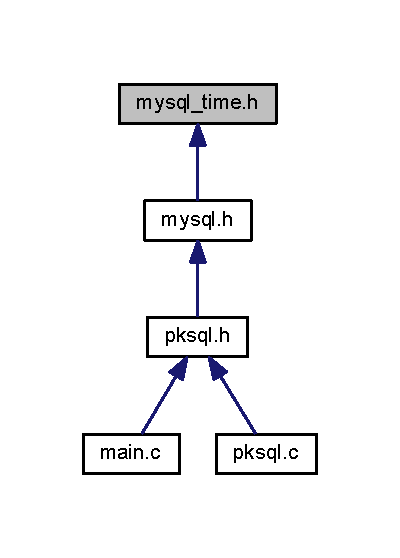
\includegraphics[width=192pt]{mysql__time_8h__dep__incl}
\end{center}
\end{figure}
\subsection*{Data Structures}
\begin{DoxyCompactItemize}
\item 
struct \hyperlink{structst__mysql__time}{st\+\_\+mysql\+\_\+time}
\end{DoxyCompactItemize}
\subsection*{Typedefs}
\begin{DoxyCompactItemize}
\item 
typedef struct \hyperlink{structst__mysql__time}{st\+\_\+mysql\+\_\+time} \hyperlink{mysql__time_8h_ac8ce1404612eae21f9a0a2595a344f48}{M\+Y\+S\+Q\+L\+\_\+\+T\+I\+M\+E}
\end{DoxyCompactItemize}
\subsection*{Enumerations}
\begin{DoxyCompactItemize}
\item 
enum \hyperlink{mysql__time_8h_aa633db8da896a5a0cc00ffcfb7477e73}{enum\+\_\+mysql\+\_\+timestamp\+\_\+type} \{ \\*
\hyperlink{mysql__time_8h_aa633db8da896a5a0cc00ffcfb7477e73ace26c6b7d67a27c905dbcd130b3bd807}{M\+Y\+S\+Q\+L\+\_\+\+T\+I\+M\+E\+S\+T\+A\+M\+P\+\_\+\+N\+O\+N\+E} = -\/2, 
\hyperlink{mysql__time_8h_aa633db8da896a5a0cc00ffcfb7477e73a3518624dcc1eaca8d816c52aa7528f72}{M\+Y\+S\+Q\+L\+\_\+\+T\+I\+M\+E\+S\+T\+A\+M\+P\+\_\+\+E\+R\+R\+O\+R} = -\/1, 
\hyperlink{mysql__time_8h_aa633db8da896a5a0cc00ffcfb7477e73a9e0845dc169b1f0056d2ffa3780c3f4e}{M\+Y\+S\+Q\+L\+\_\+\+T\+I\+M\+E\+S\+T\+A\+M\+P\+\_\+\+D\+A\+T\+E} = 0, 
\hyperlink{mysql__time_8h_aa633db8da896a5a0cc00ffcfb7477e73a8f6d8f066ea6ea77280c6a0baf063ce1}{M\+Y\+S\+Q\+L\+\_\+\+T\+I\+M\+E\+S\+T\+A\+M\+P\+\_\+\+D\+A\+T\+E\+T\+I\+M\+E} = 1, 
\\*
\hyperlink{mysql__time_8h_aa633db8da896a5a0cc00ffcfb7477e73a283c50fa3c62a2e17ad5173442edbbb9}{M\+Y\+S\+Q\+L\+\_\+\+T\+I\+M\+E\+S\+T\+A\+M\+P\+\_\+\+T\+I\+M\+E} = 2
 \}
\end{DoxyCompactItemize}


\subsection{Typedef Documentation}
\hypertarget{mysql__time_8h_ac8ce1404612eae21f9a0a2595a344f48}{}\index{mysql\+\_\+time.\+h@{mysql\+\_\+time.\+h}!M\+Y\+S\+Q\+L\+\_\+\+T\+I\+M\+E@{M\+Y\+S\+Q\+L\+\_\+\+T\+I\+M\+E}}
\index{M\+Y\+S\+Q\+L\+\_\+\+T\+I\+M\+E@{M\+Y\+S\+Q\+L\+\_\+\+T\+I\+M\+E}!mysql\+\_\+time.\+h@{mysql\+\_\+time.\+h}}
\subsubsection[{M\+Y\+S\+Q\+L\+\_\+\+T\+I\+M\+E}]{\setlength{\rightskip}{0pt plus 5cm}typedef struct {\bf st\+\_\+mysql\+\_\+time}  {\bf M\+Y\+S\+Q\+L\+\_\+\+T\+I\+M\+E}}\label{mysql__time_8h_ac8ce1404612eae21f9a0a2595a344f48}


\subsection{Enumeration Type Documentation}
\hypertarget{mysql__time_8h_aa633db8da896a5a0cc00ffcfb7477e73}{}\index{mysql\+\_\+time.\+h@{mysql\+\_\+time.\+h}!enum\+\_\+mysql\+\_\+timestamp\+\_\+type@{enum\+\_\+mysql\+\_\+timestamp\+\_\+type}}
\index{enum\+\_\+mysql\+\_\+timestamp\+\_\+type@{enum\+\_\+mysql\+\_\+timestamp\+\_\+type}!mysql\+\_\+time.\+h@{mysql\+\_\+time.\+h}}
\subsubsection[{enum\+\_\+mysql\+\_\+timestamp\+\_\+type}]{\setlength{\rightskip}{0pt plus 5cm}enum {\bf enum\+\_\+mysql\+\_\+timestamp\+\_\+type}}\label{mysql__time_8h_aa633db8da896a5a0cc00ffcfb7477e73}
\begin{Desc}
\item[Enumerator]\par
\begin{description}
\index{M\+Y\+S\+Q\+L\+\_\+\+T\+I\+M\+E\+S\+T\+A\+M\+P\+\_\+\+N\+O\+N\+E@{M\+Y\+S\+Q\+L\+\_\+\+T\+I\+M\+E\+S\+T\+A\+M\+P\+\_\+\+N\+O\+N\+E}!mysql\+\_\+time.\+h@{mysql\+\_\+time.\+h}}\index{mysql\+\_\+time.\+h@{mysql\+\_\+time.\+h}!M\+Y\+S\+Q\+L\+\_\+\+T\+I\+M\+E\+S\+T\+A\+M\+P\+\_\+\+N\+O\+N\+E@{M\+Y\+S\+Q\+L\+\_\+\+T\+I\+M\+E\+S\+T\+A\+M\+P\+\_\+\+N\+O\+N\+E}}\item[{\em 
\hypertarget{mysql__time_8h_aa633db8da896a5a0cc00ffcfb7477e73ace26c6b7d67a27c905dbcd130b3bd807}{}M\+Y\+S\+Q\+L\+\_\+\+T\+I\+M\+E\+S\+T\+A\+M\+P\+\_\+\+N\+O\+N\+E\label{mysql__time_8h_aa633db8da896a5a0cc00ffcfb7477e73ace26c6b7d67a27c905dbcd130b3bd807}
}]\index{M\+Y\+S\+Q\+L\+\_\+\+T\+I\+M\+E\+S\+T\+A\+M\+P\+\_\+\+E\+R\+R\+O\+R@{M\+Y\+S\+Q\+L\+\_\+\+T\+I\+M\+E\+S\+T\+A\+M\+P\+\_\+\+E\+R\+R\+O\+R}!mysql\+\_\+time.\+h@{mysql\+\_\+time.\+h}}\index{mysql\+\_\+time.\+h@{mysql\+\_\+time.\+h}!M\+Y\+S\+Q\+L\+\_\+\+T\+I\+M\+E\+S\+T\+A\+M\+P\+\_\+\+E\+R\+R\+O\+R@{M\+Y\+S\+Q\+L\+\_\+\+T\+I\+M\+E\+S\+T\+A\+M\+P\+\_\+\+E\+R\+R\+O\+R}}\item[{\em 
\hypertarget{mysql__time_8h_aa633db8da896a5a0cc00ffcfb7477e73a3518624dcc1eaca8d816c52aa7528f72}{}M\+Y\+S\+Q\+L\+\_\+\+T\+I\+M\+E\+S\+T\+A\+M\+P\+\_\+\+E\+R\+R\+O\+R\label{mysql__time_8h_aa633db8da896a5a0cc00ffcfb7477e73a3518624dcc1eaca8d816c52aa7528f72}
}]\index{M\+Y\+S\+Q\+L\+\_\+\+T\+I\+M\+E\+S\+T\+A\+M\+P\+\_\+\+D\+A\+T\+E@{M\+Y\+S\+Q\+L\+\_\+\+T\+I\+M\+E\+S\+T\+A\+M\+P\+\_\+\+D\+A\+T\+E}!mysql\+\_\+time.\+h@{mysql\+\_\+time.\+h}}\index{mysql\+\_\+time.\+h@{mysql\+\_\+time.\+h}!M\+Y\+S\+Q\+L\+\_\+\+T\+I\+M\+E\+S\+T\+A\+M\+P\+\_\+\+D\+A\+T\+E@{M\+Y\+S\+Q\+L\+\_\+\+T\+I\+M\+E\+S\+T\+A\+M\+P\+\_\+\+D\+A\+T\+E}}\item[{\em 
\hypertarget{mysql__time_8h_aa633db8da896a5a0cc00ffcfb7477e73a9e0845dc169b1f0056d2ffa3780c3f4e}{}M\+Y\+S\+Q\+L\+\_\+\+T\+I\+M\+E\+S\+T\+A\+M\+P\+\_\+\+D\+A\+T\+E\label{mysql__time_8h_aa633db8da896a5a0cc00ffcfb7477e73a9e0845dc169b1f0056d2ffa3780c3f4e}
}]\index{M\+Y\+S\+Q\+L\+\_\+\+T\+I\+M\+E\+S\+T\+A\+M\+P\+\_\+\+D\+A\+T\+E\+T\+I\+M\+E@{M\+Y\+S\+Q\+L\+\_\+\+T\+I\+M\+E\+S\+T\+A\+M\+P\+\_\+\+D\+A\+T\+E\+T\+I\+M\+E}!mysql\+\_\+time.\+h@{mysql\+\_\+time.\+h}}\index{mysql\+\_\+time.\+h@{mysql\+\_\+time.\+h}!M\+Y\+S\+Q\+L\+\_\+\+T\+I\+M\+E\+S\+T\+A\+M\+P\+\_\+\+D\+A\+T\+E\+T\+I\+M\+E@{M\+Y\+S\+Q\+L\+\_\+\+T\+I\+M\+E\+S\+T\+A\+M\+P\+\_\+\+D\+A\+T\+E\+T\+I\+M\+E}}\item[{\em 
\hypertarget{mysql__time_8h_aa633db8da896a5a0cc00ffcfb7477e73a8f6d8f066ea6ea77280c6a0baf063ce1}{}M\+Y\+S\+Q\+L\+\_\+\+T\+I\+M\+E\+S\+T\+A\+M\+P\+\_\+\+D\+A\+T\+E\+T\+I\+M\+E\label{mysql__time_8h_aa633db8da896a5a0cc00ffcfb7477e73a8f6d8f066ea6ea77280c6a0baf063ce1}
}]\index{M\+Y\+S\+Q\+L\+\_\+\+T\+I\+M\+E\+S\+T\+A\+M\+P\+\_\+\+T\+I\+M\+E@{M\+Y\+S\+Q\+L\+\_\+\+T\+I\+M\+E\+S\+T\+A\+M\+P\+\_\+\+T\+I\+M\+E}!mysql\+\_\+time.\+h@{mysql\+\_\+time.\+h}}\index{mysql\+\_\+time.\+h@{mysql\+\_\+time.\+h}!M\+Y\+S\+Q\+L\+\_\+\+T\+I\+M\+E\+S\+T\+A\+M\+P\+\_\+\+T\+I\+M\+E@{M\+Y\+S\+Q\+L\+\_\+\+T\+I\+M\+E\+S\+T\+A\+M\+P\+\_\+\+T\+I\+M\+E}}\item[{\em 
\hypertarget{mysql__time_8h_aa633db8da896a5a0cc00ffcfb7477e73a283c50fa3c62a2e17ad5173442edbbb9}{}M\+Y\+S\+Q\+L\+\_\+\+T\+I\+M\+E\+S\+T\+A\+M\+P\+\_\+\+T\+I\+M\+E\label{mysql__time_8h_aa633db8da896a5a0cc00ffcfb7477e73a283c50fa3c62a2e17ad5173442edbbb9}
}]\end{description}
\end{Desc}

\hypertarget{mysql__version_8h}{}\section{mysql\+\_\+version.\+h File Reference}
\label{mysql__version_8h}\index{mysql\+\_\+version.\+h@{mysql\+\_\+version.\+h}}
This graph shows which files directly or indirectly include this file\+:\nopagebreak
\begin{figure}[H]
\begin{center}
\leavevmode
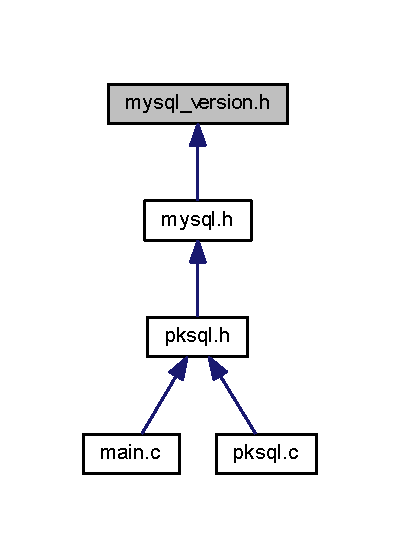
\includegraphics[width=192pt]{mysql__version_8h__dep__incl}
\end{center}
\end{figure}
\subsection*{Macros}
\begin{DoxyCompactItemize}
\item 
\#define \hyperlink{mysql__version_8h_a277f7abca2044f354abe265252cb9252}{P\+R\+O\+T\+O\+C\+O\+L\+\_\+\+V\+E\+R\+S\+I\+O\+N}~@P\+R\+O\+T\+O\+C\+O\+L\+\_\+\+V\+E\+R\+S\+I\+O\+N@
\item 
\#define \hyperlink{mysql__version_8h_aa6e02cfeaeead8c40aa987e1e8fb09f2}{M\+Y\+S\+Q\+L\+\_\+\+S\+E\+R\+V\+E\+R\+\_\+\+V\+E\+R\+S\+I\+O\+N}~\char`\"{}@S\+E\+R\+V\+E\+R\+\_\+\+V\+E\+R\+S\+I\+O\+N@\char`\"{}
\item 
\#define \hyperlink{mysql__version_8h_a454aa0373776ab09062008bc25201ccd}{M\+Y\+S\+Q\+L\+\_\+\+V\+E\+R\+S\+I\+O\+N\+\_\+\+I\+D}~@S\+E\+R\+V\+E\+R\+\_\+\+V\+E\+R\+S\+I\+O\+N\+\_\+\+I\+D@
\item 
\#define \hyperlink{mysql__version_8h_abc9bd37560a5a41068660f851ef8cffa}{M\+Y\+S\+Q\+L\+\_\+\+P\+O\+R\+T}~@M\+Y\+S\+Q\+L\+\_\+\+T\+C\+P\+\_\+\+P\+O\+R\+T@
\item 
\#define \hyperlink{mysql__version_8h_aa66a4b0e512eee5d4b7112d447800499}{M\+Y\+S\+Q\+L\+\_\+\+P\+O\+R\+T\+\_\+\+D\+E\+F\+A\+U\+L\+T}~@M\+Y\+S\+Q\+L\+\_\+\+T\+C\+P\+\_\+\+P\+O\+R\+T\+\_\+\+D\+E\+F\+A\+U\+L\+T@
\item 
\#define \hyperlink{mysql__version_8h_a823d7ef533256ea45254c827092277f5}{M\+Y\+S\+Q\+L\+\_\+\+U\+N\+I\+X\+\_\+\+A\+D\+D\+R}~\char`\"{}@M\+Y\+S\+Q\+L\+\_\+\+U\+N\+I\+X\+\_\+\+A\+D\+D\+R@\char`\"{}
\item 
\#define \hyperlink{mysql__version_8h_a45a1e94653add2650c118275c454c946}{M\+Y\+S\+Q\+L\+\_\+\+C\+O\+N\+F\+I\+G\+\_\+\+N\+A\+M\+E}~\char`\"{}my\char`\"{}
\item 
\#define \hyperlink{mysql__version_8h_a1e916f17f80d1dc94c3da4209034b9a6}{M\+Y\+S\+Q\+L\+\_\+\+C\+O\+M\+P\+I\+L\+A\+T\+I\+O\+N\+\_\+\+C\+O\+M\+M\+E\+N\+T}~\char`\"{}@C\+O\+M\+P\+I\+L\+A\+T\+I\+O\+N\+\_\+\+C\+O\+M\+M\+E\+N\+T@\char`\"{}
\item 
\#define \hyperlink{mysql__version_8h_a7e2d3394ff9eb3db0c1e43dec855736c}{L\+I\+B\+M\+Y\+S\+Q\+L\+\_\+\+V\+E\+R\+S\+I\+O\+N}~\char`\"{}@V\+E\+R\+S\+I\+O\+N@\char`\"{}
\item 
\#define \hyperlink{mysql__version_8h_a8105988db6057bf671b5a5f206439d9f}{L\+I\+B\+M\+Y\+S\+Q\+L\+\_\+\+V\+E\+R\+S\+I\+O\+N\+\_\+\+I\+D}~@\hyperlink{mysql__version_8h_a454aa0373776ab09062008bc25201ccd}{M\+Y\+S\+Q\+L\+\_\+\+V\+E\+R\+S\+I\+O\+N\+\_\+\+I\+D}@
\item 
\#define \hyperlink{mysql__version_8h_a5c614f0c43289cf27b3358d928440a36}{L\+I\+C\+E\+N\+S\+E}~G\+P\+L
\end{DoxyCompactItemize}


\subsection{Macro Definition Documentation}
\hypertarget{mysql__version_8h_a7e2d3394ff9eb3db0c1e43dec855736c}{}\index{mysql\+\_\+version.\+h@{mysql\+\_\+version.\+h}!L\+I\+B\+M\+Y\+S\+Q\+L\+\_\+\+V\+E\+R\+S\+I\+O\+N@{L\+I\+B\+M\+Y\+S\+Q\+L\+\_\+\+V\+E\+R\+S\+I\+O\+N}}
\index{L\+I\+B\+M\+Y\+S\+Q\+L\+\_\+\+V\+E\+R\+S\+I\+O\+N@{L\+I\+B\+M\+Y\+S\+Q\+L\+\_\+\+V\+E\+R\+S\+I\+O\+N}!mysql\+\_\+version.\+h@{mysql\+\_\+version.\+h}}
\subsubsection[{L\+I\+B\+M\+Y\+S\+Q\+L\+\_\+\+V\+E\+R\+S\+I\+O\+N}]{\setlength{\rightskip}{0pt plus 5cm}\#define L\+I\+B\+M\+Y\+S\+Q\+L\+\_\+\+V\+E\+R\+S\+I\+O\+N~\char`\"{}@V\+E\+R\+S\+I\+O\+N@\char`\"{}}\label{mysql__version_8h_a7e2d3394ff9eb3db0c1e43dec855736c}
\hypertarget{mysql__version_8h_a8105988db6057bf671b5a5f206439d9f}{}\index{mysql\+\_\+version.\+h@{mysql\+\_\+version.\+h}!L\+I\+B\+M\+Y\+S\+Q\+L\+\_\+\+V\+E\+R\+S\+I\+O\+N\+\_\+\+I\+D@{L\+I\+B\+M\+Y\+S\+Q\+L\+\_\+\+V\+E\+R\+S\+I\+O\+N\+\_\+\+I\+D}}
\index{L\+I\+B\+M\+Y\+S\+Q\+L\+\_\+\+V\+E\+R\+S\+I\+O\+N\+\_\+\+I\+D@{L\+I\+B\+M\+Y\+S\+Q\+L\+\_\+\+V\+E\+R\+S\+I\+O\+N\+\_\+\+I\+D}!mysql\+\_\+version.\+h@{mysql\+\_\+version.\+h}}
\subsubsection[{L\+I\+B\+M\+Y\+S\+Q\+L\+\_\+\+V\+E\+R\+S\+I\+O\+N\+\_\+\+I\+D}]{\setlength{\rightskip}{0pt plus 5cm}\#define L\+I\+B\+M\+Y\+S\+Q\+L\+\_\+\+V\+E\+R\+S\+I\+O\+N\+\_\+\+I\+D~@{\bf M\+Y\+S\+Q\+L\+\_\+\+V\+E\+R\+S\+I\+O\+N\+\_\+\+I\+D}@}\label{mysql__version_8h_a8105988db6057bf671b5a5f206439d9f}
\hypertarget{mysql__version_8h_a5c614f0c43289cf27b3358d928440a36}{}\index{mysql\+\_\+version.\+h@{mysql\+\_\+version.\+h}!L\+I\+C\+E\+N\+S\+E@{L\+I\+C\+E\+N\+S\+E}}
\index{L\+I\+C\+E\+N\+S\+E@{L\+I\+C\+E\+N\+S\+E}!mysql\+\_\+version.\+h@{mysql\+\_\+version.\+h}}
\subsubsection[{L\+I\+C\+E\+N\+S\+E}]{\setlength{\rightskip}{0pt plus 5cm}\#define L\+I\+C\+E\+N\+S\+E~G\+P\+L}\label{mysql__version_8h_a5c614f0c43289cf27b3358d928440a36}
\hypertarget{mysql__version_8h_a1e916f17f80d1dc94c3da4209034b9a6}{}\index{mysql\+\_\+version.\+h@{mysql\+\_\+version.\+h}!M\+Y\+S\+Q\+L\+\_\+\+C\+O\+M\+P\+I\+L\+A\+T\+I\+O\+N\+\_\+\+C\+O\+M\+M\+E\+N\+T@{M\+Y\+S\+Q\+L\+\_\+\+C\+O\+M\+P\+I\+L\+A\+T\+I\+O\+N\+\_\+\+C\+O\+M\+M\+E\+N\+T}}
\index{M\+Y\+S\+Q\+L\+\_\+\+C\+O\+M\+P\+I\+L\+A\+T\+I\+O\+N\+\_\+\+C\+O\+M\+M\+E\+N\+T@{M\+Y\+S\+Q\+L\+\_\+\+C\+O\+M\+P\+I\+L\+A\+T\+I\+O\+N\+\_\+\+C\+O\+M\+M\+E\+N\+T}!mysql\+\_\+version.\+h@{mysql\+\_\+version.\+h}}
\subsubsection[{M\+Y\+S\+Q\+L\+\_\+\+C\+O\+M\+P\+I\+L\+A\+T\+I\+O\+N\+\_\+\+C\+O\+M\+M\+E\+N\+T}]{\setlength{\rightskip}{0pt plus 5cm}\#define M\+Y\+S\+Q\+L\+\_\+\+C\+O\+M\+P\+I\+L\+A\+T\+I\+O\+N\+\_\+\+C\+O\+M\+M\+E\+N\+T~\char`\"{}@C\+O\+M\+P\+I\+L\+A\+T\+I\+O\+N\+\_\+\+C\+O\+M\+M\+E\+N\+T@\char`\"{}}\label{mysql__version_8h_a1e916f17f80d1dc94c3da4209034b9a6}
\hypertarget{mysql__version_8h_a45a1e94653add2650c118275c454c946}{}\index{mysql\+\_\+version.\+h@{mysql\+\_\+version.\+h}!M\+Y\+S\+Q\+L\+\_\+\+C\+O\+N\+F\+I\+G\+\_\+\+N\+A\+M\+E@{M\+Y\+S\+Q\+L\+\_\+\+C\+O\+N\+F\+I\+G\+\_\+\+N\+A\+M\+E}}
\index{M\+Y\+S\+Q\+L\+\_\+\+C\+O\+N\+F\+I\+G\+\_\+\+N\+A\+M\+E@{M\+Y\+S\+Q\+L\+\_\+\+C\+O\+N\+F\+I\+G\+\_\+\+N\+A\+M\+E}!mysql\+\_\+version.\+h@{mysql\+\_\+version.\+h}}
\subsubsection[{M\+Y\+S\+Q\+L\+\_\+\+C\+O\+N\+F\+I\+G\+\_\+\+N\+A\+M\+E}]{\setlength{\rightskip}{0pt plus 5cm}\#define M\+Y\+S\+Q\+L\+\_\+\+C\+O\+N\+F\+I\+G\+\_\+\+N\+A\+M\+E~\char`\"{}my\char`\"{}}\label{mysql__version_8h_a45a1e94653add2650c118275c454c946}
\hypertarget{mysql__version_8h_abc9bd37560a5a41068660f851ef8cffa}{}\index{mysql\+\_\+version.\+h@{mysql\+\_\+version.\+h}!M\+Y\+S\+Q\+L\+\_\+\+P\+O\+R\+T@{M\+Y\+S\+Q\+L\+\_\+\+P\+O\+R\+T}}
\index{M\+Y\+S\+Q\+L\+\_\+\+P\+O\+R\+T@{M\+Y\+S\+Q\+L\+\_\+\+P\+O\+R\+T}!mysql\+\_\+version.\+h@{mysql\+\_\+version.\+h}}
\subsubsection[{M\+Y\+S\+Q\+L\+\_\+\+P\+O\+R\+T}]{\setlength{\rightskip}{0pt plus 5cm}\#define M\+Y\+S\+Q\+L\+\_\+\+P\+O\+R\+T~@M\+Y\+S\+Q\+L\+\_\+\+T\+C\+P\+\_\+\+P\+O\+R\+T@}\label{mysql__version_8h_abc9bd37560a5a41068660f851ef8cffa}
\hypertarget{mysql__version_8h_aa66a4b0e512eee5d4b7112d447800499}{}\index{mysql\+\_\+version.\+h@{mysql\+\_\+version.\+h}!M\+Y\+S\+Q\+L\+\_\+\+P\+O\+R\+T\+\_\+\+D\+E\+F\+A\+U\+L\+T@{M\+Y\+S\+Q\+L\+\_\+\+P\+O\+R\+T\+\_\+\+D\+E\+F\+A\+U\+L\+T}}
\index{M\+Y\+S\+Q\+L\+\_\+\+P\+O\+R\+T\+\_\+\+D\+E\+F\+A\+U\+L\+T@{M\+Y\+S\+Q\+L\+\_\+\+P\+O\+R\+T\+\_\+\+D\+E\+F\+A\+U\+L\+T}!mysql\+\_\+version.\+h@{mysql\+\_\+version.\+h}}
\subsubsection[{M\+Y\+S\+Q\+L\+\_\+\+P\+O\+R\+T\+\_\+\+D\+E\+F\+A\+U\+L\+T}]{\setlength{\rightskip}{0pt plus 5cm}\#define M\+Y\+S\+Q\+L\+\_\+\+P\+O\+R\+T\+\_\+\+D\+E\+F\+A\+U\+L\+T~@M\+Y\+S\+Q\+L\+\_\+\+T\+C\+P\+\_\+\+P\+O\+R\+T\+\_\+\+D\+E\+F\+A\+U\+L\+T@}\label{mysql__version_8h_aa66a4b0e512eee5d4b7112d447800499}
\hypertarget{mysql__version_8h_aa6e02cfeaeead8c40aa987e1e8fb09f2}{}\index{mysql\+\_\+version.\+h@{mysql\+\_\+version.\+h}!M\+Y\+S\+Q\+L\+\_\+\+S\+E\+R\+V\+E\+R\+\_\+\+V\+E\+R\+S\+I\+O\+N@{M\+Y\+S\+Q\+L\+\_\+\+S\+E\+R\+V\+E\+R\+\_\+\+V\+E\+R\+S\+I\+O\+N}}
\index{M\+Y\+S\+Q\+L\+\_\+\+S\+E\+R\+V\+E\+R\+\_\+\+V\+E\+R\+S\+I\+O\+N@{M\+Y\+S\+Q\+L\+\_\+\+S\+E\+R\+V\+E\+R\+\_\+\+V\+E\+R\+S\+I\+O\+N}!mysql\+\_\+version.\+h@{mysql\+\_\+version.\+h}}
\subsubsection[{M\+Y\+S\+Q\+L\+\_\+\+S\+E\+R\+V\+E\+R\+\_\+\+V\+E\+R\+S\+I\+O\+N}]{\setlength{\rightskip}{0pt plus 5cm}\#define M\+Y\+S\+Q\+L\+\_\+\+S\+E\+R\+V\+E\+R\+\_\+\+V\+E\+R\+S\+I\+O\+N~\char`\"{}@S\+E\+R\+V\+E\+R\+\_\+\+V\+E\+R\+S\+I\+O\+N@\char`\"{}}\label{mysql__version_8h_aa6e02cfeaeead8c40aa987e1e8fb09f2}
\hypertarget{mysql__version_8h_a823d7ef533256ea45254c827092277f5}{}\index{mysql\+\_\+version.\+h@{mysql\+\_\+version.\+h}!M\+Y\+S\+Q\+L\+\_\+\+U\+N\+I\+X\+\_\+\+A\+D\+D\+R@{M\+Y\+S\+Q\+L\+\_\+\+U\+N\+I\+X\+\_\+\+A\+D\+D\+R}}
\index{M\+Y\+S\+Q\+L\+\_\+\+U\+N\+I\+X\+\_\+\+A\+D\+D\+R@{M\+Y\+S\+Q\+L\+\_\+\+U\+N\+I\+X\+\_\+\+A\+D\+D\+R}!mysql\+\_\+version.\+h@{mysql\+\_\+version.\+h}}
\subsubsection[{M\+Y\+S\+Q\+L\+\_\+\+U\+N\+I\+X\+\_\+\+A\+D\+D\+R}]{\setlength{\rightskip}{0pt plus 5cm}\#define M\+Y\+S\+Q\+L\+\_\+\+U\+N\+I\+X\+\_\+\+A\+D\+D\+R~\char`\"{}@M\+Y\+S\+Q\+L\+\_\+\+U\+N\+I\+X\+\_\+\+A\+D\+D\+R@\char`\"{}}\label{mysql__version_8h_a823d7ef533256ea45254c827092277f5}
\hypertarget{mysql__version_8h_a454aa0373776ab09062008bc25201ccd}{}\index{mysql\+\_\+version.\+h@{mysql\+\_\+version.\+h}!M\+Y\+S\+Q\+L\+\_\+\+V\+E\+R\+S\+I\+O\+N\+\_\+\+I\+D@{M\+Y\+S\+Q\+L\+\_\+\+V\+E\+R\+S\+I\+O\+N\+\_\+\+I\+D}}
\index{M\+Y\+S\+Q\+L\+\_\+\+V\+E\+R\+S\+I\+O\+N\+\_\+\+I\+D@{M\+Y\+S\+Q\+L\+\_\+\+V\+E\+R\+S\+I\+O\+N\+\_\+\+I\+D}!mysql\+\_\+version.\+h@{mysql\+\_\+version.\+h}}
\subsubsection[{M\+Y\+S\+Q\+L\+\_\+\+V\+E\+R\+S\+I\+O\+N\+\_\+\+I\+D}]{\setlength{\rightskip}{0pt plus 5cm}\#define M\+Y\+S\+Q\+L\+\_\+\+V\+E\+R\+S\+I\+O\+N\+\_\+\+I\+D~@S\+E\+R\+V\+E\+R\+\_\+\+V\+E\+R\+S\+I\+O\+N\+\_\+\+I\+D@}\label{mysql__version_8h_a454aa0373776ab09062008bc25201ccd}
\hypertarget{mysql__version_8h_a277f7abca2044f354abe265252cb9252}{}\index{mysql\+\_\+version.\+h@{mysql\+\_\+version.\+h}!P\+R\+O\+T\+O\+C\+O\+L\+\_\+\+V\+E\+R\+S\+I\+O\+N@{P\+R\+O\+T\+O\+C\+O\+L\+\_\+\+V\+E\+R\+S\+I\+O\+N}}
\index{P\+R\+O\+T\+O\+C\+O\+L\+\_\+\+V\+E\+R\+S\+I\+O\+N@{P\+R\+O\+T\+O\+C\+O\+L\+\_\+\+V\+E\+R\+S\+I\+O\+N}!mysql\+\_\+version.\+h@{mysql\+\_\+version.\+h}}
\subsubsection[{P\+R\+O\+T\+O\+C\+O\+L\+\_\+\+V\+E\+R\+S\+I\+O\+N}]{\setlength{\rightskip}{0pt plus 5cm}\#define P\+R\+O\+T\+O\+C\+O\+L\+\_\+\+V\+E\+R\+S\+I\+O\+N~@P\+R\+O\+T\+O\+C\+O\+L\+\_\+\+V\+E\+R\+S\+I\+O\+N@}\label{mysql__version_8h_a277f7abca2044f354abe265252cb9252}

\section{U\+:/\+I\+C\+T/7th\+\_\+semester/bpri2/code/my\+Ethernut/rs485/src/my\+Trash.c File Reference}
\label{my_trash_8c}\index{U\+:/\+I\+C\+T/7th\+\_\+semester/bpri2/code/my\+Ethernut/rs485/src/my\+Trash.\+c@{U\+:/\+I\+C\+T/7th\+\_\+semester/bpri2/code/my\+Ethernut/rs485/src/my\+Trash.\+c}}

\hypertarget{pksql_8c}{}\section{pksql.\+c File Reference}
\label{pksql_8c}\index{pksql.\+c@{pksql.\+c}}
{\ttfamily \#include \char`\"{}pksql.\+h\char`\"{}}\\*
Include dependency graph for pksql.\+c\+:\nopagebreak
\begin{figure}[H]
\begin{center}
\leavevmode
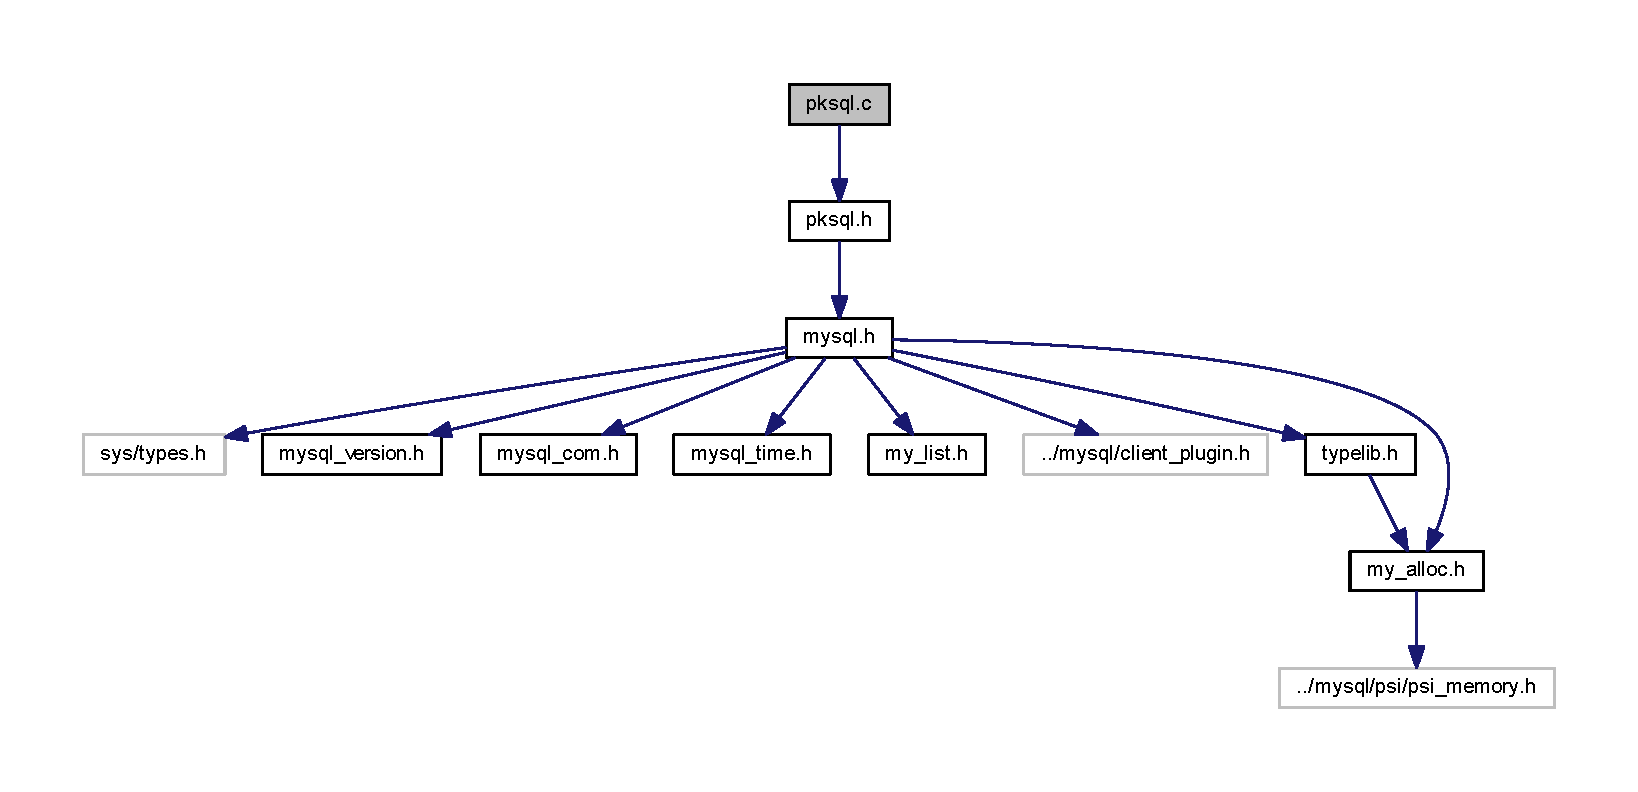
\includegraphics[width=350pt]{pksql_8c__incl}
\end{center}
\end{figure}
\subsection*{Functions}
\begin{DoxyCompactItemize}
\item 
B\+O\+O\+L \hyperlink{pksql_8c_a8109537902d55c45705c5210417b2e6c}{display\+All\+From\+Table} (char $\ast$my\+Table, int my\+I\+D)
\item 
B\+O\+O\+L \hyperlink{pksql_8c_a3bcc2d3f20cb923e4eaa70e5d2195359}{My\+S\+Q\+L\+Connect} ()
\item 
B\+O\+O\+L \hyperlink{pksql_8c_acfcbcaa2f6f2cbc3d57bd53a4d673d13}{insert\+M\+M\+Data} (char $\ast$my\+Table)
\item 
B\+O\+O\+L \hyperlink{pksql_8c_a4d7efb4557ce7bcce2efd0590058fcfd}{insert\+Into\+Table} (char $\ast$my\+Table, char $\ast$machine, int r131, int r132, int r133, int r134, int r135)
\item 
B\+O\+O\+L \hyperlink{pksql_8c_a556b31f3837e7d905955a67804f47451}{insert\+Time\+Stamp} (char $\ast$my\+Table, char $\ast$column)
\end{DoxyCompactItemize}


\subsection{Function Documentation}
\hypertarget{pksql_8c_a8109537902d55c45705c5210417b2e6c}{}\index{pksql.\+c@{pksql.\+c}!display\+All\+From\+Table@{display\+All\+From\+Table}}
\index{display\+All\+From\+Table@{display\+All\+From\+Table}!pksql.\+c@{pksql.\+c}}
\subsubsection[{display\+All\+From\+Table(char $\ast$my\+Table, int my\+I\+D)}]{\setlength{\rightskip}{0pt plus 5cm}B\+O\+O\+L display\+All\+From\+Table (
\begin{DoxyParamCaption}
\item[{char $\ast$}]{my\+Table, }
\item[{int}]{my\+I\+D}
\end{DoxyParamCaption}
)}\label{pksql_8c_a8109537902d55c45705c5210417b2e6c}


Here is the call graph for this function\+:\nopagebreak
\begin{figure}[H]
\begin{center}
\leavevmode
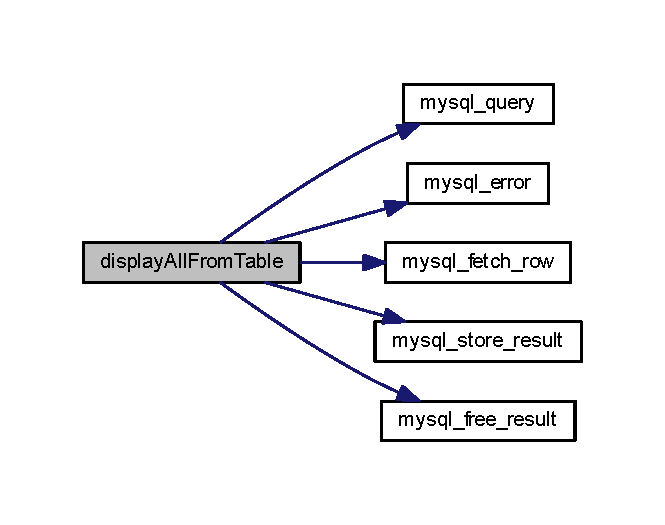
\includegraphics[width=319pt]{pksql_8c_a8109537902d55c45705c5210417b2e6c_cgraph}
\end{center}
\end{figure}


\hypertarget{pksql_8c_a4d7efb4557ce7bcce2efd0590058fcfd}{}\index{pksql.\+c@{pksql.\+c}!insert\+Into\+Table@{insert\+Into\+Table}}
\index{insert\+Into\+Table@{insert\+Into\+Table}!pksql.\+c@{pksql.\+c}}
\subsubsection[{insert\+Into\+Table(char $\ast$my\+Table, char $\ast$machine, int r131, int r132, int r133, int r134, int r135)}]{\setlength{\rightskip}{0pt plus 5cm}B\+O\+O\+L insert\+Into\+Table (
\begin{DoxyParamCaption}
\item[{char $\ast$}]{my\+Table, }
\item[{char $\ast$}]{machine, }
\item[{int}]{r131, }
\item[{int}]{r132, }
\item[{int}]{r133, }
\item[{int}]{r134, }
\item[{int}]{r135}
\end{DoxyParamCaption}
)}\label{pksql_8c_a4d7efb4557ce7bcce2efd0590058fcfd}


Here is the call graph for this function\+:\nopagebreak
\begin{figure}[H]
\begin{center}
\leavevmode
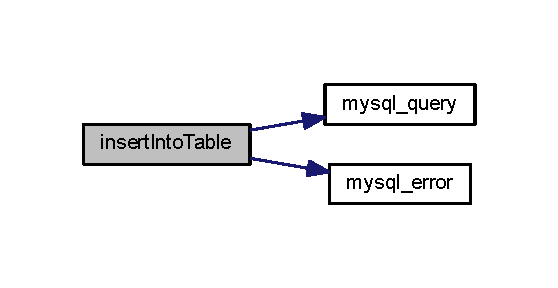
\includegraphics[width=268pt]{pksql_8c_a4d7efb4557ce7bcce2efd0590058fcfd_cgraph}
\end{center}
\end{figure}


\hypertarget{pksql_8c_acfcbcaa2f6f2cbc3d57bd53a4d673d13}{}\index{pksql.\+c@{pksql.\+c}!insert\+M\+M\+Data@{insert\+M\+M\+Data}}
\index{insert\+M\+M\+Data@{insert\+M\+M\+Data}!pksql.\+c@{pksql.\+c}}
\subsubsection[{insert\+M\+M\+Data(char $\ast$my\+Table)}]{\setlength{\rightskip}{0pt plus 5cm}B\+O\+O\+L insert\+M\+M\+Data (
\begin{DoxyParamCaption}
\item[{char $\ast$}]{my\+Table}
\end{DoxyParamCaption}
)}\label{pksql_8c_acfcbcaa2f6f2cbc3d57bd53a4d673d13}


Here is the call graph for this function\+:\nopagebreak
\begin{figure}[H]
\begin{center}
\leavevmode
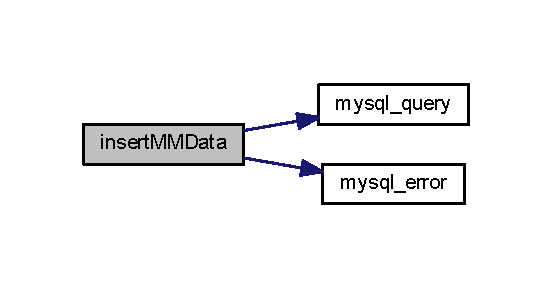
\includegraphics[width=265pt]{pksql_8c_acfcbcaa2f6f2cbc3d57bd53a4d673d13_cgraph}
\end{center}
\end{figure}


\hypertarget{pksql_8c_a556b31f3837e7d905955a67804f47451}{}\index{pksql.\+c@{pksql.\+c}!insert\+Time\+Stamp@{insert\+Time\+Stamp}}
\index{insert\+Time\+Stamp@{insert\+Time\+Stamp}!pksql.\+c@{pksql.\+c}}
\subsubsection[{insert\+Time\+Stamp(char $\ast$my\+Table, char $\ast$column)}]{\setlength{\rightskip}{0pt plus 5cm}B\+O\+O\+L insert\+Time\+Stamp (
\begin{DoxyParamCaption}
\item[{char $\ast$}]{my\+Table, }
\item[{char $\ast$}]{column}
\end{DoxyParamCaption}
)}\label{pksql_8c_a556b31f3837e7d905955a67804f47451}


Here is the call graph for this function\+:\nopagebreak
\begin{figure}[H]
\begin{center}
\leavevmode
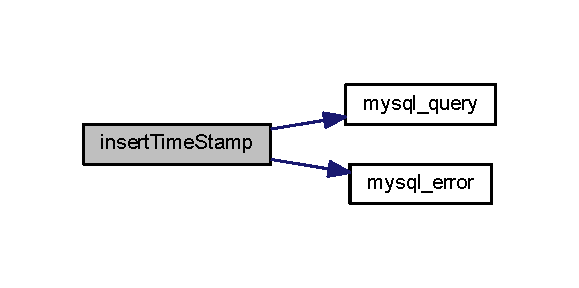
\includegraphics[width=278pt]{pksql_8c_a556b31f3837e7d905955a67804f47451_cgraph}
\end{center}
\end{figure}


\hypertarget{pksql_8c_a3bcc2d3f20cb923e4eaa70e5d2195359}{}\index{pksql.\+c@{pksql.\+c}!My\+S\+Q\+L\+Connect@{My\+S\+Q\+L\+Connect}}
\index{My\+S\+Q\+L\+Connect@{My\+S\+Q\+L\+Connect}!pksql.\+c@{pksql.\+c}}
\subsubsection[{My\+S\+Q\+L\+Connect()}]{\setlength{\rightskip}{0pt plus 5cm}B\+O\+O\+L My\+S\+Q\+L\+Connect (
\begin{DoxyParamCaption}
{}
\end{DoxyParamCaption}
)}\label{pksql_8c_a3bcc2d3f20cb923e4eaa70e5d2195359}


Here is the call graph for this function\+:\nopagebreak
\begin{figure}[H]
\begin{center}
\leavevmode
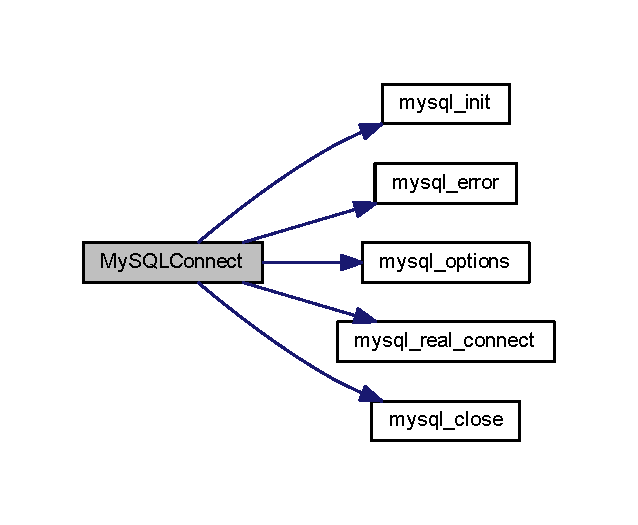
\includegraphics[width=306pt]{pksql_8c_a3bcc2d3f20cb923e4eaa70e5d2195359_cgraph}
\end{center}
\end{figure}



\hypertarget{pksql_8h}{}\section{pksql.\+h File Reference}
\label{pksql_8h}\index{pksql.\+h@{pksql.\+h}}
{\ttfamily \#include \char`\"{}mysql.\+h\char`\"{}}\\*
Include dependency graph for pksql.\+h\+:\nopagebreak
\begin{figure}[H]
\begin{center}
\leavevmode
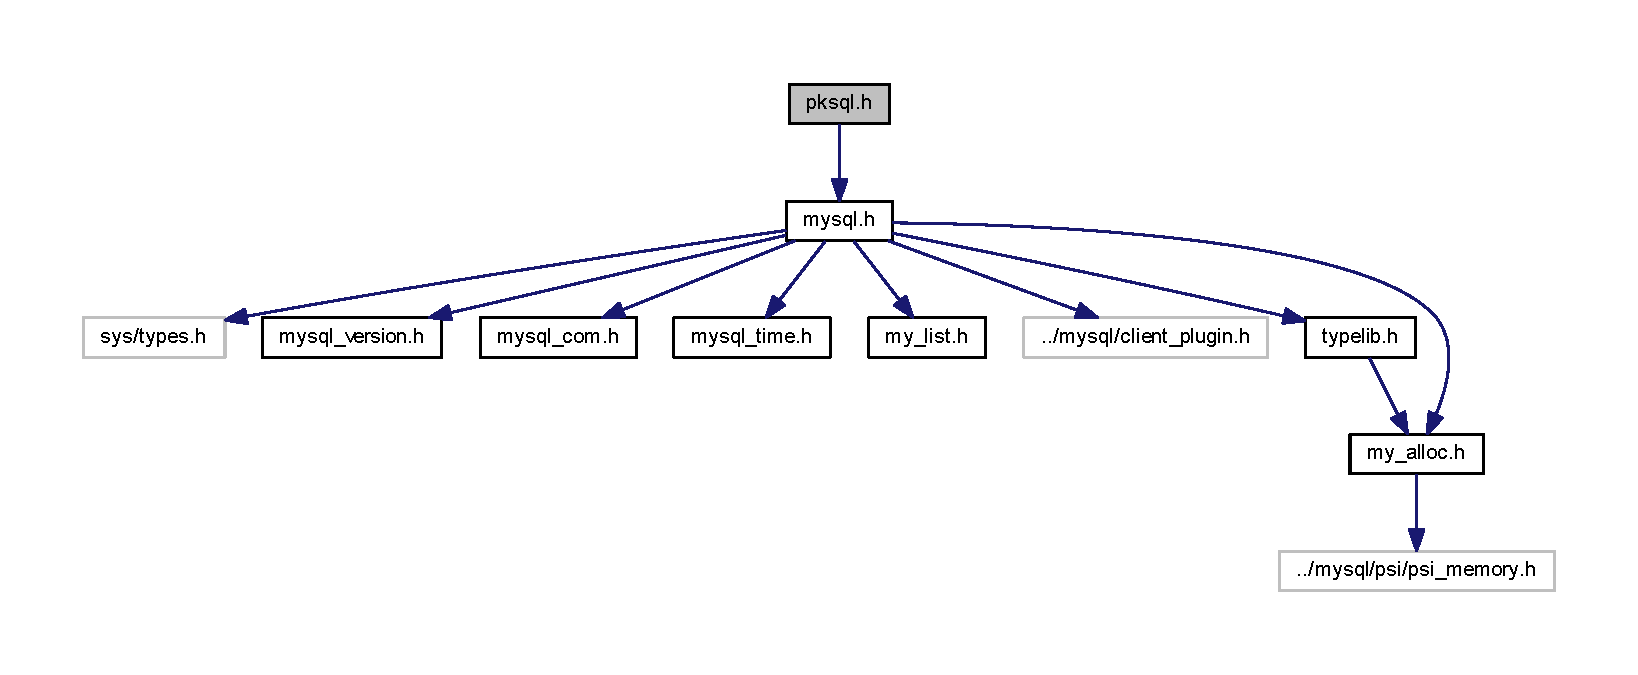
\includegraphics[width=350pt]{pksql_8h__incl}
\end{center}
\end{figure}
This graph shows which files directly or indirectly include this file\+:\nopagebreak
\begin{figure}[H]
\begin{center}
\leavevmode
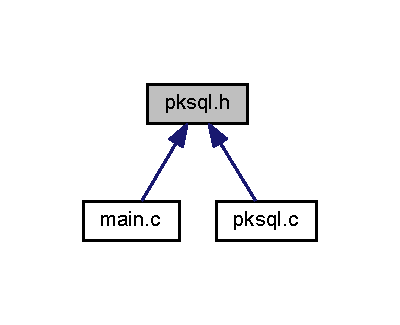
\includegraphics[width=192pt]{pksql_8h__dep__incl}
\end{center}
\end{figure}
\subsection*{Macros}
\begin{DoxyCompactItemize}
\item 
\#define \hyperlink{pksql_8h_a7485233945887459d65005a7669104a6}{D\+B\+N\+A\+M\+E}~\char`\"{}maintenance\char`\"{}
\item 
\#define \hyperlink{pksql_8h_acfc12278a87672861e438f8841a7a713}{L\+O\+C\+A\+L\+H\+O\+S\+T}~\char`\"{}127.\+0.\+0.\+1\char`\"{}
\item 
\#define \hyperlink{pksql_8h_a8bfbbf31b7d3c07215440d18a064b7f4}{U\+S\+E\+R}~\char`\"{}root\char`\"{}
\item 
\#define \hyperlink{pksql_8h_aba5c54fadff8d880b1945dde87496e31}{P\+A\+S\+S}~\char`\"{}admin\char`\"{}
\end{DoxyCompactItemize}
\subsection*{Functions}
\begin{DoxyCompactItemize}
\item 
B\+O\+O\+L \hyperlink{pksql_8h_a8b909a723dc6d0092907c796276a08ec}{display\+All\+From\+Table} (char $\ast$table, int id)
\item 
B\+O\+O\+L \hyperlink{pksql_8h_a3bcc2d3f20cb923e4eaa70e5d2195359}{My\+S\+Q\+L\+Connect} ()
\item 
B\+O\+O\+L \hyperlink{pksql_8h_acfcbcaa2f6f2cbc3d57bd53a4d673d13}{insert\+M\+M\+Data} (char $\ast$my\+Table)
\item 
B\+O\+O\+L \hyperlink{pksql_8h_aa0890e5a0157dcc938d6fb7b43e9c7f1}{insert\+Into\+Table} (char $\ast$table, char $\ast$machine, int r131, int r132, int r133, int r134, int r135)
\item 
B\+O\+O\+L \hyperlink{pksql_8h_adbba85b021fda9020527f0128df3967f}{insert\+Time\+Stamp} (char $\ast$table, char $\ast$column)
\end{DoxyCompactItemize}
\subsection*{Variables}
\begin{DoxyCompactItemize}
\item 
char \hyperlink{pksql_8h_a73c8ca1876a58205f1826be52730108a}{sz\+S\+Q\+L} \mbox{[}1024\mbox{]}
\item 
\hyperlink{mysql_8h_a42e5b5e53a1263817a59e42e219feca6}{M\+Y\+S\+Q\+L} $\ast$ \hyperlink{pksql_8h_af823d2b4dfbe0ce4969622878ccaab48}{g\+\_\+p\+My\+S\+Q\+L}
\item 
static char $\ast$ \hyperlink{pksql_8h_a7efa7eb2a557374c6f6bef7cf729744d}{g\+\_\+p\+My\+S\+Q\+L\+Options} \mbox{[}$\,$\mbox{]}
\item 
static char $\ast$ \hyperlink{pksql_8h_afff3fd7dbfa3cc8cbb449cdf72b7d413}{g\+\_\+p\+My\+S\+Q\+L\+Option\+Groups} \mbox{[}$\,$\mbox{]}
\item 
unsigned short \hyperlink{pksql_8h_aded104d45b5a4e3f8c13631ef0108f58}{mm\+Values} \mbox{[}1024\mbox{]}
\item 
unsigned char $\ast$ \hyperlink{pksql_8h_a128323d9598c2ea56dd6ae1e32a94210}{mm\+Values\+Ptr} \mbox{[}1024\mbox{]}
\end{DoxyCompactItemize}


\subsection{Macro Definition Documentation}
\hypertarget{pksql_8h_a7485233945887459d65005a7669104a6}{}\index{pksql.\+h@{pksql.\+h}!D\+B\+N\+A\+M\+E@{D\+B\+N\+A\+M\+E}}
\index{D\+B\+N\+A\+M\+E@{D\+B\+N\+A\+M\+E}!pksql.\+h@{pksql.\+h}}
\subsubsection[{D\+B\+N\+A\+M\+E}]{\setlength{\rightskip}{0pt plus 5cm}\#define D\+B\+N\+A\+M\+E~\char`\"{}maintenance\char`\"{}}\label{pksql_8h_a7485233945887459d65005a7669104a6}
\hypertarget{pksql_8h_acfc12278a87672861e438f8841a7a713}{}\index{pksql.\+h@{pksql.\+h}!L\+O\+C\+A\+L\+H\+O\+S\+T@{L\+O\+C\+A\+L\+H\+O\+S\+T}}
\index{L\+O\+C\+A\+L\+H\+O\+S\+T@{L\+O\+C\+A\+L\+H\+O\+S\+T}!pksql.\+h@{pksql.\+h}}
\subsubsection[{L\+O\+C\+A\+L\+H\+O\+S\+T}]{\setlength{\rightskip}{0pt plus 5cm}\#define L\+O\+C\+A\+L\+H\+O\+S\+T~\char`\"{}127.\+0.\+0.\+1\char`\"{}}\label{pksql_8h_acfc12278a87672861e438f8841a7a713}
\hypertarget{pksql_8h_aba5c54fadff8d880b1945dde87496e31}{}\index{pksql.\+h@{pksql.\+h}!P\+A\+S\+S@{P\+A\+S\+S}}
\index{P\+A\+S\+S@{P\+A\+S\+S}!pksql.\+h@{pksql.\+h}}
\subsubsection[{P\+A\+S\+S}]{\setlength{\rightskip}{0pt plus 5cm}\#define P\+A\+S\+S~\char`\"{}admin\char`\"{}}\label{pksql_8h_aba5c54fadff8d880b1945dde87496e31}
\hypertarget{pksql_8h_a8bfbbf31b7d3c07215440d18a064b7f4}{}\index{pksql.\+h@{pksql.\+h}!U\+S\+E\+R@{U\+S\+E\+R}}
\index{U\+S\+E\+R@{U\+S\+E\+R}!pksql.\+h@{pksql.\+h}}
\subsubsection[{U\+S\+E\+R}]{\setlength{\rightskip}{0pt plus 5cm}\#define U\+S\+E\+R~\char`\"{}root\char`\"{}}\label{pksql_8h_a8bfbbf31b7d3c07215440d18a064b7f4}


\subsection{Function Documentation}
\hypertarget{pksql_8h_a8b909a723dc6d0092907c796276a08ec}{}\index{pksql.\+h@{pksql.\+h}!display\+All\+From\+Table@{display\+All\+From\+Table}}
\index{display\+All\+From\+Table@{display\+All\+From\+Table}!pksql.\+h@{pksql.\+h}}
\subsubsection[{display\+All\+From\+Table(char $\ast$table, int id)}]{\setlength{\rightskip}{0pt plus 5cm}B\+O\+O\+L display\+All\+From\+Table (
\begin{DoxyParamCaption}
\item[{char $\ast$}]{table, }
\item[{int}]{id}
\end{DoxyParamCaption}
)}\label{pksql_8h_a8b909a723dc6d0092907c796276a08ec}


Here is the call graph for this function\+:\nopagebreak
\begin{figure}[H]
\begin{center}
\leavevmode
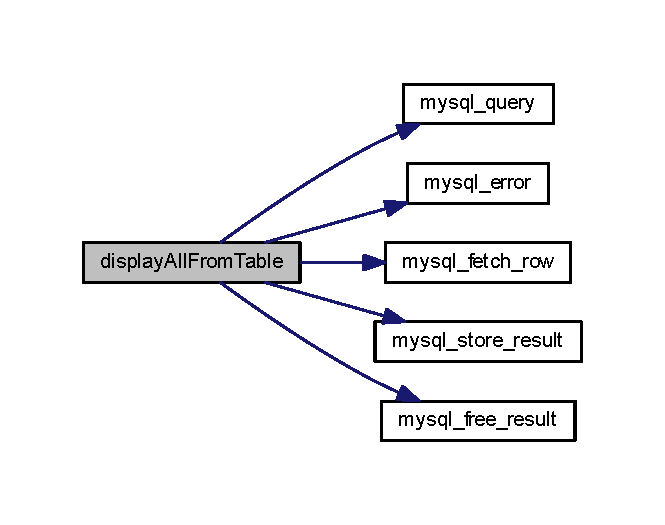
\includegraphics[width=319pt]{pksql_8h_a8b909a723dc6d0092907c796276a08ec_cgraph}
\end{center}
\end{figure}


\hypertarget{pksql_8h_aa0890e5a0157dcc938d6fb7b43e9c7f1}{}\index{pksql.\+h@{pksql.\+h}!insert\+Into\+Table@{insert\+Into\+Table}}
\index{insert\+Into\+Table@{insert\+Into\+Table}!pksql.\+h@{pksql.\+h}}
\subsubsection[{insert\+Into\+Table(char $\ast$table, char $\ast$machine, int r131, int r132, int r133, int r134, int r135)}]{\setlength{\rightskip}{0pt plus 5cm}B\+O\+O\+L insert\+Into\+Table (
\begin{DoxyParamCaption}
\item[{char $\ast$}]{table, }
\item[{char $\ast$}]{machine, }
\item[{int}]{r131, }
\item[{int}]{r132, }
\item[{int}]{r133, }
\item[{int}]{r134, }
\item[{int}]{r135}
\end{DoxyParamCaption}
)}\label{pksql_8h_aa0890e5a0157dcc938d6fb7b43e9c7f1}


Here is the call graph for this function\+:\nopagebreak
\begin{figure}[H]
\begin{center}
\leavevmode
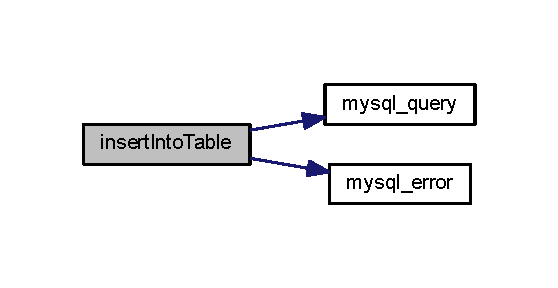
\includegraphics[width=268pt]{pksql_8h_aa0890e5a0157dcc938d6fb7b43e9c7f1_cgraph}
\end{center}
\end{figure}


\hypertarget{pksql_8h_acfcbcaa2f6f2cbc3d57bd53a4d673d13}{}\index{pksql.\+h@{pksql.\+h}!insert\+M\+M\+Data@{insert\+M\+M\+Data}}
\index{insert\+M\+M\+Data@{insert\+M\+M\+Data}!pksql.\+h@{pksql.\+h}}
\subsubsection[{insert\+M\+M\+Data(char $\ast$my\+Table)}]{\setlength{\rightskip}{0pt plus 5cm}B\+O\+O\+L insert\+M\+M\+Data (
\begin{DoxyParamCaption}
\item[{char $\ast$}]{my\+Table}
\end{DoxyParamCaption}
)}\label{pksql_8h_acfcbcaa2f6f2cbc3d57bd53a4d673d13}


Here is the call graph for this function\+:\nopagebreak
\begin{figure}[H]
\begin{center}
\leavevmode
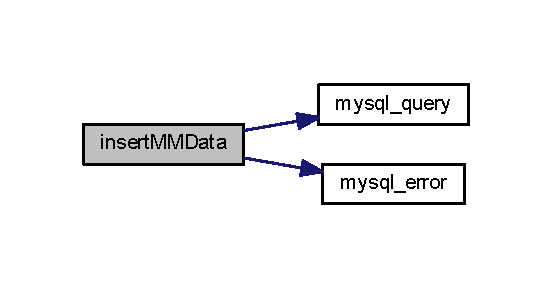
\includegraphics[width=265pt]{pksql_8h_acfcbcaa2f6f2cbc3d57bd53a4d673d13_cgraph}
\end{center}
\end{figure}


\hypertarget{pksql_8h_adbba85b021fda9020527f0128df3967f}{}\index{pksql.\+h@{pksql.\+h}!insert\+Time\+Stamp@{insert\+Time\+Stamp}}
\index{insert\+Time\+Stamp@{insert\+Time\+Stamp}!pksql.\+h@{pksql.\+h}}
\subsubsection[{insert\+Time\+Stamp(char $\ast$table, char $\ast$column)}]{\setlength{\rightskip}{0pt plus 5cm}B\+O\+O\+L insert\+Time\+Stamp (
\begin{DoxyParamCaption}
\item[{char $\ast$}]{table, }
\item[{char $\ast$}]{column}
\end{DoxyParamCaption}
)}\label{pksql_8h_adbba85b021fda9020527f0128df3967f}


Here is the call graph for this function\+:\nopagebreak
\begin{figure}[H]
\begin{center}
\leavevmode
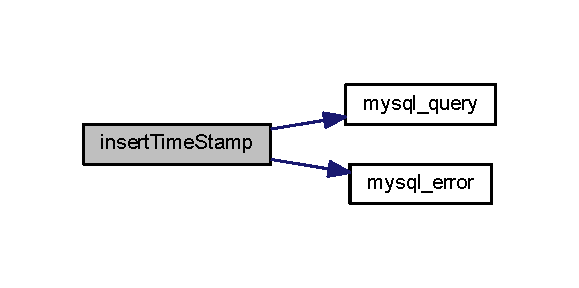
\includegraphics[width=278pt]{pksql_8h_adbba85b021fda9020527f0128df3967f_cgraph}
\end{center}
\end{figure}


\hypertarget{pksql_8h_a3bcc2d3f20cb923e4eaa70e5d2195359}{}\index{pksql.\+h@{pksql.\+h}!My\+S\+Q\+L\+Connect@{My\+S\+Q\+L\+Connect}}
\index{My\+S\+Q\+L\+Connect@{My\+S\+Q\+L\+Connect}!pksql.\+h@{pksql.\+h}}
\subsubsection[{My\+S\+Q\+L\+Connect()}]{\setlength{\rightskip}{0pt plus 5cm}B\+O\+O\+L My\+S\+Q\+L\+Connect (
\begin{DoxyParamCaption}
{}
\end{DoxyParamCaption}
)}\label{pksql_8h_a3bcc2d3f20cb923e4eaa70e5d2195359}


Here is the call graph for this function\+:\nopagebreak
\begin{figure}[H]
\begin{center}
\leavevmode
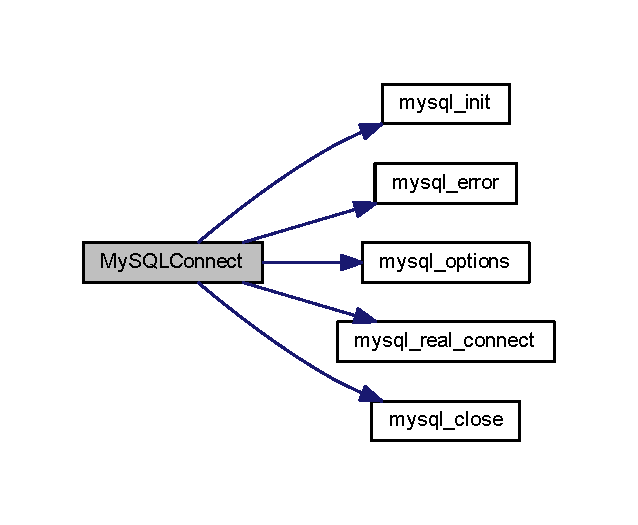
\includegraphics[width=306pt]{pksql_8h_a3bcc2d3f20cb923e4eaa70e5d2195359_cgraph}
\end{center}
\end{figure}




\subsection{Variable Documentation}
\hypertarget{pksql_8h_af823d2b4dfbe0ce4969622878ccaab48}{}\index{pksql.\+h@{pksql.\+h}!g\+\_\+p\+My\+S\+Q\+L@{g\+\_\+p\+My\+S\+Q\+L}}
\index{g\+\_\+p\+My\+S\+Q\+L@{g\+\_\+p\+My\+S\+Q\+L}!pksql.\+h@{pksql.\+h}}
\subsubsection[{g\+\_\+p\+My\+S\+Q\+L}]{\setlength{\rightskip}{0pt plus 5cm}{\bf M\+Y\+S\+Q\+L}$\ast$ g\+\_\+p\+My\+S\+Q\+L}\label{pksql_8h_af823d2b4dfbe0ce4969622878ccaab48}
\hypertarget{pksql_8h_afff3fd7dbfa3cc8cbb449cdf72b7d413}{}\index{pksql.\+h@{pksql.\+h}!g\+\_\+p\+My\+S\+Q\+L\+Option\+Groups@{g\+\_\+p\+My\+S\+Q\+L\+Option\+Groups}}
\index{g\+\_\+p\+My\+S\+Q\+L\+Option\+Groups@{g\+\_\+p\+My\+S\+Q\+L\+Option\+Groups}!pksql.\+h@{pksql.\+h}}
\subsubsection[{g\+\_\+p\+My\+S\+Q\+L\+Option\+Groups}]{\setlength{\rightskip}{0pt plus 5cm}char$\ast$ g\+\_\+p\+My\+S\+Q\+L\+Option\+Groups\mbox{[}$\,$\mbox{]}\hspace{0.3cm}{\ttfamily [static]}}\label{pksql_8h_afff3fd7dbfa3cc8cbb449cdf72b7d413}
{\bfseries Initial value\+:}
\begin{DoxyCode}
=
\{ \textcolor{stringliteral}{"MyTimeStamp"}, NULL \}
\end{DoxyCode}
\hypertarget{pksql_8h_a7efa7eb2a557374c6f6bef7cf729744d}{}\index{pksql.\+h@{pksql.\+h}!g\+\_\+p\+My\+S\+Q\+L\+Options@{g\+\_\+p\+My\+S\+Q\+L\+Options}}
\index{g\+\_\+p\+My\+S\+Q\+L\+Options@{g\+\_\+p\+My\+S\+Q\+L\+Options}!pksql.\+h@{pksql.\+h}}
\subsubsection[{g\+\_\+p\+My\+S\+Q\+L\+Options}]{\setlength{\rightskip}{0pt plus 5cm}char$\ast$ g\+\_\+p\+My\+S\+Q\+L\+Options\mbox{[}$\,$\mbox{]}\hspace{0.3cm}{\ttfamily [static]}}\label{pksql_8h_a7efa7eb2a557374c6f6bef7cf729744d}
{\bfseries Initial value\+:}
\begin{DoxyCode}
=
\{ \textcolor{stringliteral}{"MyTimeStamp"}, \textcolor{stringliteral}{"--datadir=./data"}, \textcolor{stringliteral}{"--language=./language"}, \textcolor{stringliteral}{"--skip-innodb"}, \textcolor{stringliteral}{"--key-buffer-size=64M"}, \textcolor{stringliteral}{"
      --console"},
        NULL \}
\end{DoxyCode}
\hypertarget{pksql_8h_aded104d45b5a4e3f8c13631ef0108f58}{}\index{pksql.\+h@{pksql.\+h}!mm\+Values@{mm\+Values}}
\index{mm\+Values@{mm\+Values}!pksql.\+h@{pksql.\+h}}
\subsubsection[{mm\+Values}]{\setlength{\rightskip}{0pt plus 5cm}unsigned short mm\+Values\mbox{[}1024\mbox{]}}\label{pksql_8h_aded104d45b5a4e3f8c13631ef0108f58}
\hypertarget{pksql_8h_a128323d9598c2ea56dd6ae1e32a94210}{}\index{pksql.\+h@{pksql.\+h}!mm\+Values\+Ptr@{mm\+Values\+Ptr}}
\index{mm\+Values\+Ptr@{mm\+Values\+Ptr}!pksql.\+h@{pksql.\+h}}
\subsubsection[{mm\+Values\+Ptr}]{\setlength{\rightskip}{0pt plus 5cm}unsigned char$\ast$ mm\+Values\+Ptr\mbox{[}1024\mbox{]}}\label{pksql_8h_a128323d9598c2ea56dd6ae1e32a94210}
\hypertarget{pksql_8h_a73c8ca1876a58205f1826be52730108a}{}\index{pksql.\+h@{pksql.\+h}!sz\+S\+Q\+L@{sz\+S\+Q\+L}}
\index{sz\+S\+Q\+L@{sz\+S\+Q\+L}!pksql.\+h@{pksql.\+h}}
\subsubsection[{sz\+S\+Q\+L}]{\setlength{\rightskip}{0pt plus 5cm}char sz\+S\+Q\+L\mbox{[}1024\mbox{]}}\label{pksql_8h_a73c8ca1876a58205f1826be52730108a}

\hypertarget{targetver_8h}{}\section{targetver.\+h File Reference}
\label{targetver_8h}\index{targetver.\+h@{targetver.\+h}}
{\ttfamily \#include $<$S\+D\+K\+D\+D\+K\+Ver.\+h$>$}\\*
Include dependency graph for targetver.\+h\+:\nopagebreak
\begin{figure}[H]
\begin{center}
\leavevmode
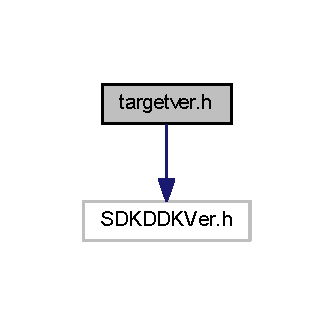
\includegraphics[width=160pt]{targetver_8h__incl}
\end{center}
\end{figure}

\hypertarget{typelib_8h}{}\section{typelib.\+h File Reference}
\label{typelib_8h}\index{typelib.\+h@{typelib.\+h}}
{\ttfamily \#include \char`\"{}my\+\_\+alloc.\+h\char`\"{}}\\*
Include dependency graph for typelib.\+h\+:\nopagebreak
\begin{figure}[H]
\begin{center}
\leavevmode
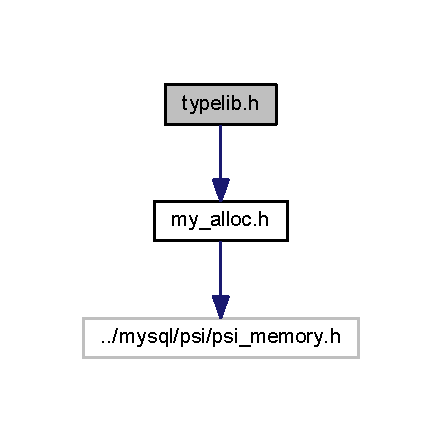
\includegraphics[width=212pt]{typelib_8h__incl}
\end{center}
\end{figure}
This graph shows which files directly or indirectly include this file\+:\nopagebreak
\begin{figure}[H]
\begin{center}
\leavevmode
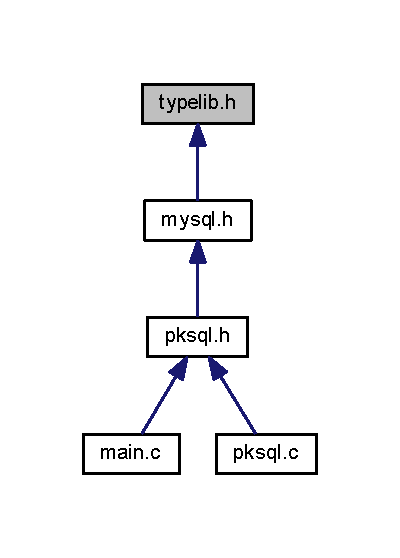
\includegraphics[width=192pt]{typelib_8h__dep__incl}
\end{center}
\end{figure}
\subsection*{Data Structures}
\begin{DoxyCompactItemize}
\item 
struct \hyperlink{structst__typelib}{st\+\_\+typelib}
\end{DoxyCompactItemize}
\subsection*{Macros}
\begin{DoxyCompactItemize}
\item 
\#define \hyperlink{typelib_8h_afb4ead8806e46e24402e5bbf0d412dc4}{F\+I\+N\+D\+\_\+\+T\+Y\+P\+E\+\_\+\+B\+A\+S\+I\+C}~0
\item 
\#define \hyperlink{typelib_8h_a60285ac2997d01b487c39aed17e96c2f}{F\+I\+N\+D\+\_\+\+T\+Y\+P\+E\+\_\+\+N\+O\+\_\+\+P\+R\+E\+F\+I\+X}~(1 $<$$<$ 0)
\item 
\#define \hyperlink{typelib_8h_a70d837aaab543d572a28d4f712c45d42}{F\+I\+N\+D\+\_\+\+T\+Y\+P\+E\+\_\+\+N\+O\+\_\+\+O\+V\+E\+R\+W\+R\+I\+T\+E}~(1 $<$$<$ 1)
\item 
\#define \hyperlink{typelib_8h_a0c72eb6cd13589471fa2e9e4aba025cf}{F\+I\+N\+D\+\_\+\+T\+Y\+P\+E\+\_\+\+A\+L\+L\+O\+W\+\_\+\+N\+U\+M\+B\+E\+R}~(1 $<$$<$ 2)
\item 
\#define \hyperlink{typelib_8h_a9a25853cbee8966ed9cb4594ad55dbad}{F\+I\+N\+D\+\_\+\+T\+Y\+P\+E\+\_\+\+C\+O\+M\+M\+A\+\_\+\+T\+E\+R\+M}~(1 $<$$<$ 3)
\end{DoxyCompactItemize}
\subsection*{Typedefs}
\begin{DoxyCompactItemize}
\item 
typedef struct \hyperlink{structst__typelib}{st\+\_\+typelib} \hyperlink{typelib_8h_ab89ec075c5be74420fdf771c0f391876}{T\+Y\+P\+E\+L\+I\+B}
\end{DoxyCompactItemize}
\subsection*{Functions}
\begin{DoxyCompactItemize}
\item 
\hyperlink{mysql_8h_ae05bd5d3e5a75578e2f14cfeb43f07aa}{my\+\_\+ulonglong} \hyperlink{typelib_8h_a126abd11d8111639258b67db4098523c}{find\+\_\+typeset} (char $\ast$x, \hyperlink{typelib_8h_ab89ec075c5be74420fdf771c0f391876}{T\+Y\+P\+E\+L\+I\+B} $\ast$typelib, int $\ast$error\+\_\+position)
\item 
int \hyperlink{typelib_8h_a33e0461bb2a89a5df44cd3bc218eb379}{find\+\_\+type\+\_\+or\+\_\+exit} (const char $\ast$x, \hyperlink{typelib_8h_ab89ec075c5be74420fdf771c0f391876}{T\+Y\+P\+E\+L\+I\+B} $\ast$typelib, const char $\ast$option)
\item 
int \hyperlink{typelib_8h_aa467cecbd3bf70384a4254cf346c4bc2}{find\+\_\+type} (const char $\ast$x, const \hyperlink{typelib_8h_ab89ec075c5be74420fdf771c0f391876}{T\+Y\+P\+E\+L\+I\+B} $\ast$typelib, unsigned int flags)
\item 
void \hyperlink{typelib_8h_a8cd24ba8c6c554be1859f939e72fe97b}{make\+\_\+type} (char $\ast$to, unsigned int nr, \hyperlink{typelib_8h_ab89ec075c5be74420fdf771c0f391876}{T\+Y\+P\+E\+L\+I\+B} $\ast$typelib)
\item 
const char $\ast$ \hyperlink{typelib_8h_a278dd21e8caff88fbe707765cb9846be}{get\+\_\+type} (\hyperlink{typelib_8h_ab89ec075c5be74420fdf771c0f391876}{T\+Y\+P\+E\+L\+I\+B} $\ast$typelib, unsigned int nr)
\item 
\hyperlink{typelib_8h_ab89ec075c5be74420fdf771c0f391876}{T\+Y\+P\+E\+L\+I\+B} $\ast$ \hyperlink{typelib_8h_ad23e8664ccc3c0c985cf74281fb788a5}{copy\+\_\+typelib} (\hyperlink{my__alloc_8h_ac59e289b254a2c5ac634ffcedda3f823}{M\+E\+M\+\_\+\+R\+O\+O\+T} $\ast$root, \hyperlink{typelib_8h_ab89ec075c5be74420fdf771c0f391876}{T\+Y\+P\+E\+L\+I\+B} $\ast$from)
\item 
\hyperlink{mysql_8h_ae05bd5d3e5a75578e2f14cfeb43f07aa}{my\+\_\+ulonglong} \hyperlink{typelib_8h_acd9291bd5b7a11a34124dd6458705a35}{find\+\_\+set\+\_\+from\+\_\+flags} (const \hyperlink{typelib_8h_ab89ec075c5be74420fdf771c0f391876}{T\+Y\+P\+E\+L\+I\+B} $\ast$lib, unsigned int default\+\_\+name, \hyperlink{mysql_8h_ae05bd5d3e5a75578e2f14cfeb43f07aa}{my\+\_\+ulonglong} cur\+\_\+set, \hyperlink{mysql_8h_ae05bd5d3e5a75578e2f14cfeb43f07aa}{my\+\_\+ulonglong} default\+\_\+set, const char $\ast$str, unsigned int length, char $\ast$$\ast$err\+\_\+pos, unsigned int $\ast$err\+\_\+len)
\end{DoxyCompactItemize}
\subsection*{Variables}
\begin{DoxyCompactItemize}
\item 
\hyperlink{typelib_8h_ab89ec075c5be74420fdf771c0f391876}{T\+Y\+P\+E\+L\+I\+B} \hyperlink{typelib_8h_aae95b10469763a75fb4f2e56d04c5365}{sql\+\_\+protocol\+\_\+typelib}
\end{DoxyCompactItemize}


\subsection{Macro Definition Documentation}
\hypertarget{typelib_8h_a0c72eb6cd13589471fa2e9e4aba025cf}{}\index{typelib.\+h@{typelib.\+h}!F\+I\+N\+D\+\_\+\+T\+Y\+P\+E\+\_\+\+A\+L\+L\+O\+W\+\_\+\+N\+U\+M\+B\+E\+R@{F\+I\+N\+D\+\_\+\+T\+Y\+P\+E\+\_\+\+A\+L\+L\+O\+W\+\_\+\+N\+U\+M\+B\+E\+R}}
\index{F\+I\+N\+D\+\_\+\+T\+Y\+P\+E\+\_\+\+A\+L\+L\+O\+W\+\_\+\+N\+U\+M\+B\+E\+R@{F\+I\+N\+D\+\_\+\+T\+Y\+P\+E\+\_\+\+A\+L\+L\+O\+W\+\_\+\+N\+U\+M\+B\+E\+R}!typelib.\+h@{typelib.\+h}}
\subsubsection[{F\+I\+N\+D\+\_\+\+T\+Y\+P\+E\+\_\+\+A\+L\+L\+O\+W\+\_\+\+N\+U\+M\+B\+E\+R}]{\setlength{\rightskip}{0pt plus 5cm}\#define F\+I\+N\+D\+\_\+\+T\+Y\+P\+E\+\_\+\+A\+L\+L\+O\+W\+\_\+\+N\+U\+M\+B\+E\+R~(1 $<$$<$ 2)}\label{typelib_8h_a0c72eb6cd13589471fa2e9e4aba025cf}
makes {\ttfamily \hyperlink{typelib_8h_aa467cecbd3bf70384a4254cf346c4bc2}{find\+\_\+type()}} accept a number \hypertarget{typelib_8h_afb4ead8806e46e24402e5bbf0d412dc4}{}\index{typelib.\+h@{typelib.\+h}!F\+I\+N\+D\+\_\+\+T\+Y\+P\+E\+\_\+\+B\+A\+S\+I\+C@{F\+I\+N\+D\+\_\+\+T\+Y\+P\+E\+\_\+\+B\+A\+S\+I\+C}}
\index{F\+I\+N\+D\+\_\+\+T\+Y\+P\+E\+\_\+\+B\+A\+S\+I\+C@{F\+I\+N\+D\+\_\+\+T\+Y\+P\+E\+\_\+\+B\+A\+S\+I\+C}!typelib.\+h@{typelib.\+h}}
\subsubsection[{F\+I\+N\+D\+\_\+\+T\+Y\+P\+E\+\_\+\+B\+A\+S\+I\+C}]{\setlength{\rightskip}{0pt plus 5cm}\#define F\+I\+N\+D\+\_\+\+T\+Y\+P\+E\+\_\+\+B\+A\+S\+I\+C~0}\label{typelib_8h_afb4ead8806e46e24402e5bbf0d412dc4}
\hypertarget{typelib_8h_a9a25853cbee8966ed9cb4594ad55dbad}{}\index{typelib.\+h@{typelib.\+h}!F\+I\+N\+D\+\_\+\+T\+Y\+P\+E\+\_\+\+C\+O\+M\+M\+A\+\_\+\+T\+E\+R\+M@{F\+I\+N\+D\+\_\+\+T\+Y\+P\+E\+\_\+\+C\+O\+M\+M\+A\+\_\+\+T\+E\+R\+M}}
\index{F\+I\+N\+D\+\_\+\+T\+Y\+P\+E\+\_\+\+C\+O\+M\+M\+A\+\_\+\+T\+E\+R\+M@{F\+I\+N\+D\+\_\+\+T\+Y\+P\+E\+\_\+\+C\+O\+M\+M\+A\+\_\+\+T\+E\+R\+M}!typelib.\+h@{typelib.\+h}}
\subsubsection[{F\+I\+N\+D\+\_\+\+T\+Y\+P\+E\+\_\+\+C\+O\+M\+M\+A\+\_\+\+T\+E\+R\+M}]{\setlength{\rightskip}{0pt plus 5cm}\#define F\+I\+N\+D\+\_\+\+T\+Y\+P\+E\+\_\+\+C\+O\+M\+M\+A\+\_\+\+T\+E\+R\+M~(1 $<$$<$ 3)}\label{typelib_8h_a9a25853cbee8966ed9cb4594ad55dbad}
makes {\ttfamily \hyperlink{typelib_8h_aa467cecbd3bf70384a4254cf346c4bc2}{find\+\_\+type()}} treat \textquotesingle{},\textquotesingle{} as terminator \hypertarget{typelib_8h_a70d837aaab543d572a28d4f712c45d42}{}\index{typelib.\+h@{typelib.\+h}!F\+I\+N\+D\+\_\+\+T\+Y\+P\+E\+\_\+\+N\+O\+\_\+\+O\+V\+E\+R\+W\+R\+I\+T\+E@{F\+I\+N\+D\+\_\+\+T\+Y\+P\+E\+\_\+\+N\+O\+\_\+\+O\+V\+E\+R\+W\+R\+I\+T\+E}}
\index{F\+I\+N\+D\+\_\+\+T\+Y\+P\+E\+\_\+\+N\+O\+\_\+\+O\+V\+E\+R\+W\+R\+I\+T\+E@{F\+I\+N\+D\+\_\+\+T\+Y\+P\+E\+\_\+\+N\+O\+\_\+\+O\+V\+E\+R\+W\+R\+I\+T\+E}!typelib.\+h@{typelib.\+h}}
\subsubsection[{F\+I\+N\+D\+\_\+\+T\+Y\+P\+E\+\_\+\+N\+O\+\_\+\+O\+V\+E\+R\+W\+R\+I\+T\+E}]{\setlength{\rightskip}{0pt plus 5cm}\#define F\+I\+N\+D\+\_\+\+T\+Y\+P\+E\+\_\+\+N\+O\+\_\+\+O\+V\+E\+R\+W\+R\+I\+T\+E~(1 $<$$<$ 1)}\label{typelib_8h_a70d837aaab543d572a28d4f712c45d42}
always implicitely on, so unused, but old code may pass it \hypertarget{typelib_8h_a60285ac2997d01b487c39aed17e96c2f}{}\index{typelib.\+h@{typelib.\+h}!F\+I\+N\+D\+\_\+\+T\+Y\+P\+E\+\_\+\+N\+O\+\_\+\+P\+R\+E\+F\+I\+X@{F\+I\+N\+D\+\_\+\+T\+Y\+P\+E\+\_\+\+N\+O\+\_\+\+P\+R\+E\+F\+I\+X}}
\index{F\+I\+N\+D\+\_\+\+T\+Y\+P\+E\+\_\+\+N\+O\+\_\+\+P\+R\+E\+F\+I\+X@{F\+I\+N\+D\+\_\+\+T\+Y\+P\+E\+\_\+\+N\+O\+\_\+\+P\+R\+E\+F\+I\+X}!typelib.\+h@{typelib.\+h}}
\subsubsection[{F\+I\+N\+D\+\_\+\+T\+Y\+P\+E\+\_\+\+N\+O\+\_\+\+P\+R\+E\+F\+I\+X}]{\setlength{\rightskip}{0pt plus 5cm}\#define F\+I\+N\+D\+\_\+\+T\+Y\+P\+E\+\_\+\+N\+O\+\_\+\+P\+R\+E\+F\+I\+X~(1 $<$$<$ 0)}\label{typelib_8h_a60285ac2997d01b487c39aed17e96c2f}
makes {\ttfamily \hyperlink{typelib_8h_aa467cecbd3bf70384a4254cf346c4bc2}{find\+\_\+type()}} require the whole name, no prefix 

\subsection{Typedef Documentation}
\hypertarget{typelib_8h_ab89ec075c5be74420fdf771c0f391876}{}\index{typelib.\+h@{typelib.\+h}!T\+Y\+P\+E\+L\+I\+B@{T\+Y\+P\+E\+L\+I\+B}}
\index{T\+Y\+P\+E\+L\+I\+B@{T\+Y\+P\+E\+L\+I\+B}!typelib.\+h@{typelib.\+h}}
\subsubsection[{T\+Y\+P\+E\+L\+I\+B}]{\setlength{\rightskip}{0pt plus 5cm}typedef struct {\bf st\+\_\+typelib}  {\bf T\+Y\+P\+E\+L\+I\+B}}\label{typelib_8h_ab89ec075c5be74420fdf771c0f391876}


\subsection{Function Documentation}
\hypertarget{typelib_8h_ad23e8664ccc3c0c985cf74281fb788a5}{}\index{typelib.\+h@{typelib.\+h}!copy\+\_\+typelib@{copy\+\_\+typelib}}
\index{copy\+\_\+typelib@{copy\+\_\+typelib}!typelib.\+h@{typelib.\+h}}
\subsubsection[{copy\+\_\+typelib(\+M\+E\+M\+\_\+\+R\+O\+O\+T $\ast$root, T\+Y\+P\+E\+L\+I\+B $\ast$from)}]{\setlength{\rightskip}{0pt plus 5cm}{\bf T\+Y\+P\+E\+L\+I\+B}$\ast$ copy\+\_\+typelib (
\begin{DoxyParamCaption}
\item[{{\bf M\+E\+M\+\_\+\+R\+O\+O\+T} $\ast$}]{root, }
\item[{{\bf T\+Y\+P\+E\+L\+I\+B} $\ast$}]{from}
\end{DoxyParamCaption}
)}\label{typelib_8h_ad23e8664ccc3c0c985cf74281fb788a5}
\hypertarget{typelib_8h_acd9291bd5b7a11a34124dd6458705a35}{}\index{typelib.\+h@{typelib.\+h}!find\+\_\+set\+\_\+from\+\_\+flags@{find\+\_\+set\+\_\+from\+\_\+flags}}
\index{find\+\_\+set\+\_\+from\+\_\+flags@{find\+\_\+set\+\_\+from\+\_\+flags}!typelib.\+h@{typelib.\+h}}
\subsubsection[{find\+\_\+set\+\_\+from\+\_\+flags(const T\+Y\+P\+E\+L\+I\+B $\ast$lib, unsigned int default\+\_\+name, my\+\_\+ulonglong cur\+\_\+set, my\+\_\+ulonglong default\+\_\+set, const char $\ast$str, unsigned int length, char $\ast$$\ast$err\+\_\+pos, unsigned int $\ast$err\+\_\+len)}]{\setlength{\rightskip}{0pt plus 5cm}{\bf my\+\_\+ulonglong} find\+\_\+set\+\_\+from\+\_\+flags (
\begin{DoxyParamCaption}
\item[{const {\bf T\+Y\+P\+E\+L\+I\+B} $\ast$}]{lib, }
\item[{unsigned int}]{default\+\_\+name, }
\item[{{\bf my\+\_\+ulonglong}}]{cur\+\_\+set, }
\item[{{\bf my\+\_\+ulonglong}}]{default\+\_\+set, }
\item[{const char $\ast$}]{str, }
\item[{unsigned int}]{length, }
\item[{char $\ast$$\ast$}]{err\+\_\+pos, }
\item[{unsigned int $\ast$}]{err\+\_\+len}
\end{DoxyParamCaption}
)}\label{typelib_8h_acd9291bd5b7a11a34124dd6458705a35}
\hypertarget{typelib_8h_aa467cecbd3bf70384a4254cf346c4bc2}{}\index{typelib.\+h@{typelib.\+h}!find\+\_\+type@{find\+\_\+type}}
\index{find\+\_\+type@{find\+\_\+type}!typelib.\+h@{typelib.\+h}}
\subsubsection[{find\+\_\+type(const char $\ast$x, const T\+Y\+P\+E\+L\+I\+B $\ast$typelib, unsigned int flags)}]{\setlength{\rightskip}{0pt plus 5cm}int find\+\_\+type (
\begin{DoxyParamCaption}
\item[{const char $\ast$}]{x, }
\item[{const {\bf T\+Y\+P\+E\+L\+I\+B} $\ast$}]{typelib, }
\item[{unsigned int}]{flags}
\end{DoxyParamCaption}
)}\label{typelib_8h_aa467cecbd3bf70384a4254cf346c4bc2}
\hypertarget{typelib_8h_a33e0461bb2a89a5df44cd3bc218eb379}{}\index{typelib.\+h@{typelib.\+h}!find\+\_\+type\+\_\+or\+\_\+exit@{find\+\_\+type\+\_\+or\+\_\+exit}}
\index{find\+\_\+type\+\_\+or\+\_\+exit@{find\+\_\+type\+\_\+or\+\_\+exit}!typelib.\+h@{typelib.\+h}}
\subsubsection[{find\+\_\+type\+\_\+or\+\_\+exit(const char $\ast$x, T\+Y\+P\+E\+L\+I\+B $\ast$typelib, const char $\ast$option)}]{\setlength{\rightskip}{0pt plus 5cm}int find\+\_\+type\+\_\+or\+\_\+exit (
\begin{DoxyParamCaption}
\item[{const char $\ast$}]{x, }
\item[{{\bf T\+Y\+P\+E\+L\+I\+B} $\ast$}]{typelib, }
\item[{const char $\ast$}]{option}
\end{DoxyParamCaption}
)}\label{typelib_8h_a33e0461bb2a89a5df44cd3bc218eb379}
\hypertarget{typelib_8h_a126abd11d8111639258b67db4098523c}{}\index{typelib.\+h@{typelib.\+h}!find\+\_\+typeset@{find\+\_\+typeset}}
\index{find\+\_\+typeset@{find\+\_\+typeset}!typelib.\+h@{typelib.\+h}}
\subsubsection[{find\+\_\+typeset(char $\ast$x, T\+Y\+P\+E\+L\+I\+B $\ast$typelib, int $\ast$error\+\_\+position)}]{\setlength{\rightskip}{0pt plus 5cm}{\bf my\+\_\+ulonglong} find\+\_\+typeset (
\begin{DoxyParamCaption}
\item[{char $\ast$}]{x, }
\item[{{\bf T\+Y\+P\+E\+L\+I\+B} $\ast$}]{typelib, }
\item[{int $\ast$}]{error\+\_\+position}
\end{DoxyParamCaption}
)}\label{typelib_8h_a126abd11d8111639258b67db4098523c}
\hypertarget{typelib_8h_a278dd21e8caff88fbe707765cb9846be}{}\index{typelib.\+h@{typelib.\+h}!get\+\_\+type@{get\+\_\+type}}
\index{get\+\_\+type@{get\+\_\+type}!typelib.\+h@{typelib.\+h}}
\subsubsection[{get\+\_\+type(\+T\+Y\+P\+E\+L\+I\+B $\ast$typelib, unsigned int nr)}]{\setlength{\rightskip}{0pt plus 5cm}const char$\ast$ get\+\_\+type (
\begin{DoxyParamCaption}
\item[{{\bf T\+Y\+P\+E\+L\+I\+B} $\ast$}]{typelib, }
\item[{unsigned int}]{nr}
\end{DoxyParamCaption}
)}\label{typelib_8h_a278dd21e8caff88fbe707765cb9846be}
\hypertarget{typelib_8h_a8cd24ba8c6c554be1859f939e72fe97b}{}\index{typelib.\+h@{typelib.\+h}!make\+\_\+type@{make\+\_\+type}}
\index{make\+\_\+type@{make\+\_\+type}!typelib.\+h@{typelib.\+h}}
\subsubsection[{make\+\_\+type(char $\ast$to, unsigned int nr, T\+Y\+P\+E\+L\+I\+B $\ast$typelib)}]{\setlength{\rightskip}{0pt plus 5cm}void make\+\_\+type (
\begin{DoxyParamCaption}
\item[{char $\ast$}]{to, }
\item[{unsigned int}]{nr, }
\item[{{\bf T\+Y\+P\+E\+L\+I\+B} $\ast$}]{typelib}
\end{DoxyParamCaption}
)}\label{typelib_8h_a8cd24ba8c6c554be1859f939e72fe97b}


\subsection{Variable Documentation}
\hypertarget{typelib_8h_aae95b10469763a75fb4f2e56d04c5365}{}\index{typelib.\+h@{typelib.\+h}!sql\+\_\+protocol\+\_\+typelib@{sql\+\_\+protocol\+\_\+typelib}}
\index{sql\+\_\+protocol\+\_\+typelib@{sql\+\_\+protocol\+\_\+typelib}!typelib.\+h@{typelib.\+h}}
\subsubsection[{sql\+\_\+protocol\+\_\+typelib}]{\setlength{\rightskip}{0pt plus 5cm}{\bf T\+Y\+P\+E\+L\+I\+B} sql\+\_\+protocol\+\_\+typelib}\label{typelib_8h_aae95b10469763a75fb4f2e56d04c5365}

%--- End generated contents ---

% Index
\backmatter
\newpage
\phantomsection
\clearemptydoublepage
\addcontentsline{toc}{chapter}{Index}
\printindex

\end{document}
